\scsectionfamily{Часть 2 Стандарта OSTIS. Смысловое представление и онтологическая систематизация знаний в интеллектуальных компьютерных системах нового поколения}
\label{part_representation}

\scsection[
    \protect\scneditors{Никифоров С.А.;Бобёр  Е.С.}
    \protect\scnmonographychapter{Глава 2.6. Языковые средства формального описания синтаксиса и денотационной семантики различных языков в интеллектуальных компьютерных системах нового поколения}
    ]{Предметная область и онтология информационных конструкций и языков}
\label{intro_lang}
\begin{SCn}
    \scnsectionheader{\currentname}
    \begin{scnstruct}
        \scniselement{раздел базы знаний}
        \begin{scnrelfromlist}{дочерний раздел}
            \scnitem{\nameref{intro_sc_code}}
            \scnitem{\nameref{intro_idtf}}
            \scnitem{\nameref{intro_scg}}
            \scnitem{\nameref{intro_scs}}
            \scnitem{\nameref{intro_scn}}
        \end{scnrelfromlist}
        \scntext{аннотация}{Поскольку предлагаемая Вашему вниманию \textit{Публикация Стандарта OSTIS-2021} представляет собой внешний текст основной части \textit{базы знаний} ostis-системы (\textit{Метасистемы IMS.ostis}), необходимо сразу во вводном разделе этого Стандарта пояснить основные принципы, лежащие в основе внутреннего представления \textit{баз знаний} в памяти \textit{ostis-систем}, а также некоторые правила и условные обозначения, используемые в оформлении внешних текстов \textit{баз знаний ostis-систем}.\\Подчеркнем, что все эти принципы, правила и условные обозначения детально рассмотрены в соответствующих разделах \textit{Стандарта OSTIS}, но некоторые из них необходимо пояснить до начала ознакомления с основными положениями \textit{Технологии OSTIS}. Фактически речь идет о кратком руководстве конечных пользователей \textit{ostis-систем}. 
        \\Прежде, чем рассматривать \textit{внутренний язык*} и \textit{внешние языки*}, используемые \textit{ostis-системами}, необходимо уточнить понятие \textit{информационной конструкции}, понятие \textit{знака}, понятие \textit{текста}, понятие \textit{языка}.\\}
        \scnheader{Предметная область информационных конструкций и языков}
        \scniselement{предметная область}
        \begin{scnhaselementrole}{класс объектов исследования}
            {информационная конструкция}
        \end{scnhaselementrole}
        \begin{scnhaselementrolelist}{класс объектов исследования}
            \scnitem{дискретная информационная конструкция} 
            \scnitem{элемент дискретной информационной конструкции} 
            \scnitem{соответствие, заданное на множестве дискретных информационных конструкций} 
            \scnitem{знак}
            \scnitem{знаковая конструкция}
            \scnitem{язык}
            \scnitem{семантически выделяемый класс дискретных информационных конструкций}
            \scnitem{язык ostis-системы}
            \scnitem{ограничитель}
            \scnitem{идентификатор}
            \scnitem{имя}
            \scnitem{предложение}
            \scnitem{sc.g-текст}
            \scnitem{sc.s-текст}
            \scnitem{sc.n-текст}
        \end{scnhaselementrolelist}
        \begin{scnhaselementrolelist}{исследуемый класс классов первичных объектов исследования}
            \scnitem{отношение, заданное на множестве элементов дискретных информационных конструкций\scnsupergroupsign}
            \scnitem{параметр, заданный на множестве дискретных информационных конструкций\scnsupergroupsign}
            \scnitem{отношение, заданное на множестве знаков\scnsupergroupsign}
            \scnitem{отношение, заданное на множестве знаковых конструкций\scnsupergroupsign}
            \scnitem{класс знаковых конструкций\scnsupergroupsign}
            \scnitem{параметр, заданный на множестве знаковых конструкций\scnsupergroupsign}
            \scnitem{отношение, заданное на множестве языков\scnsupergroupsign}
            \scnitem{параметр, заданный на множестве языков\scnsupergroupsign}
        \end{scnhaselementrolelist}
        \begin{scnhaselementrolelist}{исследуемое отношение}
            \scnitem{операционная семантика информационной конструкции*}
            \scnitem{алфавит*}
            \scnitem{ограничители*}
            \scnitem{разделители*}
            \scnitem{внешний идентификатор*}
            \scnitem{предложения*}
        \end{scnhaselementrolelist}

        \scnheader{ostis-система}
        \scnidtf{компьютерная система, построенная по Технологии OSTIS}

        \scnheader{информационная конструкция}
        \scnidtf{информация}
        \scnidtf{конструкция (структура), содержащая некоторые сведения о некоторых сущностях}
        \scntext{примечание}{Форма представления (\scnqq{изображения}, материализации), форма структуризации (синтаксическая структура), а также \textit{смысл*} (денотационная семантика) \textit{информационных конструкций} могут быть самыми различными.}
        
        \scnheader{дискретная информационная конструкция}
        \scnsubset{информационная конструкция}
        \scntext{пояснение}{Каждая \textit{дискретная информационная конструкция}  это \textit{информационная конструкция}, смысл которой задается (1) множеством элементов (синтаксически атомарных фрагментов) этой информационной конструкции, (2) алфавитом этих элементов  семейством классов синтаксически эквивалентных элементов информационной конструкции, (3) принадлежностью каждого элемента информационной конструкции соответствующему классу синтаксически эквивалентных элементов информационной конструкции, (4) конфигурацией связей инцидентности между элементами информационной конструкции.}
        \begin{scnindent}
            \scntext{следствие}{Форма представления элементов дискретной информационной конструкции для анализа её смысла не требует уточнения. Главным является (1) наличие простой процедуры выделения (сегментации) элементов дискретной информационной конструкции (2) наличие простой процедуры установления синтаксической эквивалентности разных элементов дискретной информационной конструкции и (3) наличие простой процедуры установления принадлежности каждого элемента дискретной информационной конструкции соответствующему классу синтаксически эквивалентных элементов (т.е. соответствующему элементу алфавита).}
        \end{scnindent}

        \scnheader{элемент дискретной информационной конструкции}
        \scnidtf{синтаксически атомарный фрагмент (символ), входящий в состав дискретной информационной конструкции}
        \scntext{примечание}{Поскольку дискретные информационные конструкции могут иметь общие элементы (атомарные фрагменты) и даже некоторые из них могут быть частями других информационных конструкций, элемент дискретной информационной конструкции может входить в состав сразу нескольких информационных конструкций.}\scnrelto{второй домен}{элемент дискретной информационной конструкции*}
        
        \scnheader{отношение, заданное на множестве элементов дискретных информационных конструкций\scnsupergroupsign}
        \scnhaselement{элемент дискретной информационной конструкции*}
        \begin{scnindent}
            \scnidtf{быть элементарным (синтаксически атомарным) фрагментом заданной дискретной информационной конструкции*}
            \scnidtf{быть элементом (атомарным фрагментом) заданной дискретной информационной конструкции*}
            \scnidtf{Бинарное ориентированное отношение, каждая пара которого связывает (1) знак некоторой дискретной информационной конструкции и (2) знак одного из элементов этой дискретной информационной конструкции*}
            \scnrelfrom{второй домен}{элемент дискретной информационной конструкции}
        \end{scnindent}
        \scnhaselement{синтаксическая эквивалентность элементов дискретных информационных конструкций*}
        \begin{scnindent}
            \scnidtf{быть синтаксически эквивалентными элементами (атомарными фрагментами) одной и той же или разных дискретных информационных конструкций, т.е. элементами, принадлежащими одному и тому же классу синтаксически эквивалентных элементов дискретных информационных конструкций*}
        \end{scnindent}
        \scnhaselement{инцидентность элементов дискретных информационных конструкций*}
        \begin{scnindent}
            \scniselement{бинарное ориентированное отношение\scnsupergroupsign}
            \bigskip\scntext{примечание}{Для \textit{линейных информационных конструкций} --- это последовательность элементов (символов), входящих в состав этих конструкций.\\Для дискретных информационных конструкций, конфигурация которых имеет нелинейный характер, отношение инцидентности их элементов может быть разбито на несколько частных отношений инцидентности, каждое из которых является \uline{подмножеством} объединенного отношения инцидентности. Например, для двухмерных дискретных информационных конструкций это (1) инцидентность элементов информационных конструкций \scnqq{по горизонтали} и (2) инцидентность элементов информационных конструкций по вертикали.}
        \end{scnindent}
        \scnhaselement{неэлементарный фрагмент дискретной информационной конструкции*}
        \begin{scnindent}
            \scnidtf{быть дискретной информационной конструкцией, которая является \uline{подструктурой} для заданной дискретной информационной конструкции, в состав которой входит (1) подмножество элементов заданной информационной конструкции и, соответственно, (2) подмножество пар инцидентности элементов заданной информационной конструкции.}
        \end{scnindent}
        \scnhaselement{алфавит дискретной информационной конструкции*}
        \begin{scnindent}
            \scnidtf{быть семейством попарно непересекающихся \uline{классов} синтаксически эквивалентных элементов заданной дискретной информационной конструкции*}
        \end{scnindent}
        \scnhaselement{первичная синтаксическая структура дискретной информационной конструкции*}
        \begin{scnindent}
            \scnidtf{быть \textit{графовой структурой}, которая полностью описывает конфигурацию заданной \textit{дискретной информационной конструкции} и которая включает в себя: (1) знаки всех тех классов синтаксически эквивалентных элементов, которым принадлежат элементы описываемой дискретной информационной конструкции, (2) знаки всех элементов (атомарных фрагментов) описываемой информационной конструкции, (3) пары, описывающие инцидентность элементов описываемой информационной конструкции, (4) пары, описывающие принадлежность элементов описываемой информационной конструкции соответствующим классам синтаксически эквивалентных элементов этой информационной конструкции.}
        \end{scnindent}
        \scnhaselement{синтаксическая эквивалентность дискретных информационных конструкций*}
        \begin{scnindent}
            \scntext{определение}{Дискретные информационные конструкции $\bm{Ti}$ и $\bm{Tj}$ являются синтаксически эквивалентными в том и только в том случае, если между конструкцией $\bm{Ti}$ и конструкцией $\bm{Tj}$ существует \uline{изоморфизм}, в рамках которого каждому элементу конструкции $\bm{Ti}$ соответствует синтаксически эквивалентный элемент конструкции $\bm{Tj}$, т.е. элемент, принадлежащий тому же классу синтаксически эквивалентных элементов дискретных информационных конструкций. И наоборот.}
        \end{scnindent}    
        \scnhaselement{копия дискретной информационной конструкции*}
        \begin{scnindent}
            \scnsubset{синтаксическая эквивалентность дискретных информационных конструкций*}
            \scnidtftext{определение}{быть дискретной информационной конструкцией, которая не только синтаксически эквивалентна заданной, но и содержит информацию о форме представления элементов копируемой информационной конструкции*}
        \end{scnindent}
        \scnhaselement{семантическая эквивалентность дискретных информационных конструкций*}
        \begin{scnindent}
            \scntext{определение}{Информационная конструкция $\bm{Ti}$ и информационная конструкция $\bm{Tj}$ являются \uline{семантически эквивалентными} в том и только в том случае, если \uline{каждая} сущность (в том числе, и каждая связь между сущностями), описываемая в информационной конструкции $\bm{Ti}$ описывается также и в информационной конструкции $\bm{Tj}$. И наоборот.}
        \end{scnindent}
        \scnhaselement{семантическое расширение дискретной информационной конструкции*}
        \begin{scnindent}
            \scntext{определение}{Информационная конструкция $\bm{Tj}$ является семантическим расширением информационной конструкции $\bm{Ti}$ в том и только в том случае, если \uline{каждая} сущность, описываемая в $\bm{Ti}$, описывается также и в $\bm{Tj}$, но обратное неверно.}
        \end{scnindent}
        \scnhaselement{синтаксис информационной конструкции*}
        \begin{scnindent}
            \scnidtf{синтаксическая структура информационной конструкции*}
            \scnidtf{быть синтаксической структурой для заданной информационной конструкции*}
            \scnidtf{Бинарное ориентированное отношение, каждая пара которого связывает знак некоторой информационной конструкции с синтаксической структурой этой конструкции*}
            \scnidtf{описание того, из каких частей состоит заданная информационная конструкция и как эти части (фрагменты) связаны между собой*}
            \scnrelfrom{первый домен}{информационная конструкция}
        \end{scnindent}
        \bigskip\scnhaselement{смысл*}
        \begin{scnindent}
            \scnidtf{смысл информационной конструкции*}
            \scnidtf{денотационная семантика информационной конструкции*}
            \scnidtf{семантическая (смысловая) структура информационной конструкции*}
            \scnidtf{быть семантической (смысловой) структурой для заданной информационной конструкции*}
            \scnidtf{быть смыслом заданной информационной конструкции*}
            \scnidtf{быть явным (формальным) представлением того, какие сущности описывает данная информационная конструкция и как эти сущности связаны между собой*}
            \scnidtf{Бинарное ориентированное отношение, каждая пара которого связывает некоторую информационную конструкцию с ее смыслом (смысловой структурой)*}
        \end{scnindent}
        \scnhaselement{операционная семантика информационной конструкции*}
        \begin{scnindent}
            \scnidtf{правила трансформации заданной информационной конструкции*}
            \scnidtf{описание того, на основании каких правил можно осуществлять действия по преобразования (обработке, трансформации) заданной информационной конструкции, оставляя ее в рамках класса синтаксически и семантически правильных информационных конструкций*}
            \scnidtf{Бинарное ориентированное отношение, каждая пара которого связывает знак некоторой информационной конструкции со множеством правил ее трансформации*}
        \end{scnindent}
        \scnheader{операционная семантика информационной конструкции*}
        \scnrelfrom{второй домен}{операционная семантика информационной конструкции}

        \scnheader{соответствие, заданное на множестве дискретных информационных конструкций}
        \scnhaselement{соответствие между синтаксической структурой информационной конструкции и смыслом этой конструкции*}
        \begin{scnindent}
            \scnidtf{Множество ориентированных пар, первым компонентом которых является ориентированная пара, состоящая из (1) знака синтаксической структуры некоторой информационной конструкции и (2) знака смысловой структуры этой конструкции, а вторым компонентом которых является множество ориентированных пар, связывающих фрагменты синтаксической структуры заданной информационной конструкции (которые описывают либо структуру фрагментов заданной конструкции, либо связи между фрагментами этой конструкции) с теми фрагментами смысловой структуры заданной информационной конструкции, которые семантически эквивалентны либо синтаксически представленным фрагментам заданной информационной конструкции, либо синтаксически представленным связям между такими фрагментами*}
            \scnsubset{соответствие*}
        \end{scnindent}   

        \scnheader{параметр, заданный на множестве дискретных информационных конструкций\scnsupergroupsign}
        \scnhaselement{размерность дискретных информационных конструкций\scnsupergroupsign}
        \begin{scnindent}
            \scnidtf{типология дискретных информационных конструкций, определяемая их размерностью}
            \scntext{пояснение}{Это параметр дискретных информационных конструкций, определяющий характер \uline{инцидентности} элементов таких конструкций.}
            \scnhaselement{линейная информационная конструкция}
            \begin{scnindent}
                \scnidtftext{пояснение}{дискретная информационная конструкция, каждый элемент которой может иметь не более двух инцидентных ему элементов (один слева, другой справа)}
            \end{scnindent}
            \scnhaselement{двухмерная информационная конструкция}
            \begin{scnindent}
                \scnidtftext{пояснение}{дискретная информационная конструкция, каждый элемент которой может иметь не более четырех инцидентных ему элементов (слева-справа, сверху-снизу)}
            \end{scnindent}
            \scnhaselement{трехмерная информационная конструкция}
            \begin{scnindent}
                \scnidtftext{пояснение}{дискретная информационная конструкция, каждый элемент которой может иметь не более шести инцидентных ему элементов (слева-справа, сверху-снизу, сзади-спереди)}
            \end{scnindent}
            \scnhaselement{четырехмерная информационная конструкция}
            \begin{scnindent}
                \scnidtftext{пояснение}{дискретная информационная конструкция, каждый элемент которой может иметь не более восьми инцидентных ему элементов (например, слева-справа, сверху-снизу, сзади-спереди, раньше-позже)}
            \end{scnindent}
            \scnhaselement{графовая информационная конструкция}
            \begin{scnindent}
                \scnidtftext{пояснение}{дискретная информационная конструкция, множество элементов которой разбивается на два подмножества  связки и узлы. При этом узлы могут иметь \uline{неограниченное} количество инцидентных им связок}
                \begin{scnindent}
                    \scntext{примечание}{А в некоторых графовых информационных конструкциях и связки могут иметь неограниченное количество инцидентных им других связок}
                \end{scnindent}
            \end{scnindent}
        \end{scnindent}
        \scnhaselement{типология дискретных информационных конструкций, определяемая их носителем\scnsupergroupsign}
        \begin{scnindent}
            \scnhaselement{некомпьютерная форма представления дискретных информационных конструкций}
            \begin{scnindent}
                \scnsuperset{аудио-сообщение}
                \begin{scnindent}
                    \scnidtf{речевое сообщение}
                    \scnidtf{информационная конструкция, представленная в звуковой форме}
                \end{scnindent}
                \scnsuperset{информационная конструкция, представленная на языке жестов}
                \scnsuperset{информационная конструкция, представленная в письменной форме}
                \begin{scnindent}
                    \scntext{примечание}{Конкретный вид носителя для письменной формы представления информации может быть разным  бумага, папирус, береста, камень...}
                \end{scnindent}
            \end{scnindent}
            \scnhaselement{файл}
            \begin{scnindent}
                \scnidtf{компьютерная (электронная) форма (формат) представления и хранения информационных конструкций}
                \scntext{примечание}{Представление информационных конструкций в виде файлов ориентировано на представление \uline{дискретных} (!) информационных конструкций. Поэтому \scnqq{файловое} представление недискретных информационных конструкций (например, различного рода сигналов) предполагает \scnqq{дискретизацию} таких конструкций, т.е. преобразование их в дискретные. Так преобразуются аудио-сигналы (в частности, речевые сообщения), изображения, видео-сигналы и др.}
            \end{scnindent}
        \end{scnindent}
        \scnhaselement{уровень унификации представления синтаксически эквивалентных элементов дискретных информационных конструкций\scnsupergroupsign}
        \begin{scnindent}
            \scnidtf{уровень \scnqq{членораздельности} дискретных информационных конструкций}
            \scntext{примечание}{Чем выше уровень унификации представления элементов дискретных информационных конструкций, тем проще реализуется (1) процедура выделения (сегментации) элементов дискретной информационной конструкции, (2) процедура установления синтаксической эквивалентности этих элементов и (3) процедура их распознавания, т.е. процедура установления их принадлежности соответствующим классам синтаксически эквивалентных элементов.}\scnhaselement{дискретная информационная конструкция с низким уровнем унификации представления элементов}
            \begin{scnindent}
                \scnsuperset{аудио-сообщение}
                \scnsuperset{информационная конструкция, представленная на языке жестов}
                \scnsuperset{рукопись или её копия}
            \end{scnindent}
            \scnhaselement{дискретная информационная конструкция с высоким уровнем унификации представления элементов}
            \begin{scnindent}
                \scnsuperset{печатный текст}
                \scnsuperset{файл}
            \end{scnindent}
        \end{scnindent}
        
        \scnheader{знак}
        \scntext{пояснение}{фрагмент информационной конструкции, который условно представляет (изображает) некоторую описываемую сущность, которую называют денотатом знака}
        \begin{scnsubdividing}
            \scnitem{знак, являющийся элементом дискретной информационной конструкции}
            \scnitem{знак, являющийся неатомарным фрагментом дискретной информационной конструкции}
        \end{scnsubdividing}
        \scntext{примечание}{Отсутствие знака, обозначающего некоторую сущность, не означает отсутствие самой этой сущности. Это означает только то, что мы даже не догадываемся о её существовании и, следовательно, не приступили к её исследованию.}
        
        \newpage\scnheader{отношение, заданное на множестве знаков\scnsupergroupsign}
        \scntext{примечание}{Поскольку все знаки являются дискретными информационными конструкциями, множество знаков является областью задания всех отношений, заданных на множестве дискретных информационных конструкций. Тем не менее есть как минимум одно отношение, специфичное для множества знаков.}
        \scnhaselement{синонимия знаков*}
        \begin{scnindent}
            \scntext{определение}{Знаки являются синонимичными в том и только в том случае, если они обозначают одну и ту же сущность.}
            \scntext{примечание}{Синонимичные знаки могут быть синтаксически эквивалентными, а могут и не быть таковыми.}
        \end{scnindent}
        
        \scnheader{знаковая конструкция}
        \scnsubset{дискретная информационная конструкция}
        \scnidtftext{пояснение}{дискретная информационная конструкция, которая в общем случае представляет собой конфигурацию знаков и специальных фрагментов информационной конструкции, обеспечивающих структуризацию конфигурации знаков  различного вида разделителей и ограничителей}
        \begin{scnindent}
            \scntext{примечание}{Для некоторых знаковых конструкций и даже для некоторых языков необходимость в разделителях и ограничителях может отсутствовать.}
        \end{scnindent}
        
        \scnheader{отношение, заданное на множестве знаковых конструкций\scnsupergroupsign}
        \scnhaselement{знак*}
        \begin{scnindent}
            \scnidtf{быть знаком для заданной знаковой конструкции*}
        \end{scnindent}
        \scnhaselement{разделитель знаковой конструкции*}
        \scnhaselement{разделители знаковой конструкции*}
        \begin{scnindent}
            \scnidtf{Множество всех разделителей, входящих в состав заданной знаковой конструкции*}
        \end{scnindent}
        \scnhaselement{ограничитель знаковой конструкции*}
        \scnhaselement{ограничители знаковой конструкции*}
        \scnhaselement{семантическая смежность знаковых конструкций*}
        \begin{scnindent}
            \scntext{определение}{Знаковые конструкции $\bm{Ti}$ и $\bm{Tj}$ являются смежными в том и только в том случае, если существуют синонимичные знаки $\bm{Ti}$ и $\bm{Tj}$, один из которых входит в состав конструкции $\bm{Ti}$, а второй  в состав конструкции $\bm{Tj}$}
        \end{scnindent}
        \scnhaselement{конкатенация знаковых конструкций*}
        \begin{scnindent}
            \scnidtf{декомпозиция заданной знаковой конструкции на последовательность знаковых конструкций*}
        \end{scnindent}

        \scnheader{класс знаковых конструкций\scnsupergroupsign}
        \scnhaselement{семантически элементарная знаковая конструкция}
        \begin{scnindent}
            \scnidtf{знаковая конструкция, описывающая некоторую (одну) связь между некоторыми сущностями}
        \end{scnindent}
        \scnhaselement{семантически связная знаковая конструкция}
        \begin{scnindent}
            \scnidtftext{определение}{знаковая конструкция, которую можно представить в виде конкатенации семантически элементарных знаковых конструкций, каждая из которых семантически смежна предшествующей и последующей семантически элементарной знаковой конструкции}
        \end{scnindent}
        
        \scnheader{параметр, заданный на множестве знаковых конструкций\scnsupergroupsign}
        \scnhaselement{семантическая связность знаковых конструкций\scnsupergroupsign}
        \begin{scnindent}
            \scnhaselement{семантически связная знаковая конструкция}
            \scnhaselement{семантически несвязная знаковая конструкция}
            \scnhaselementrole{пример}{\scnfilelong{В огороде бузина, а в Киеве дядька}}
        \end{scnindent}
        \scnhaselement{наличие разделителей и ограничителей\scnsupergroupsign}
        \begin{scnindent}
            \scnhaselement{знаковая конструкция, содержащая разделители и-или ограничители}
            \scnhaselement{знаковая конструкция без разделителей и ограничителей}
        \end{scnindent}

        \newpage\scnheader{язык}
        \scnidtftext{пояснение}{класс знаковых конструкций, для которого существуют (1) общие правила их построения и (2) общие правила их соотнесения с теми сущностями и конфигурациями сущностей, которые описываются (отражаются) указанными знаковыми конструкциями}
        \scnidtf{класс знаковых конструкций, эквивалентных с точки зрения правил их построения и правил их семантической интерпретации}
        \begin{scnsubdividing}
            \scnitem{язык, у которого все знаки, входящие в состав его знаковых конструкций, являются элементарными фрагментами этих конструкций}
            \begin{scnindent}
                \scntext{примечание}{Для языков такого типа существенно упрощаются методы обработки их текстов.}
            \end{scnindent}
            \scnitem{язык, у которого знаки, входящие в состав его знаковых конструкций, в общем случае не являются элементарными фрагментами этих конструкций}
        \end{scnsubdividing}
        \begin{scnsubdividing}
            \scnitem{язык, знаковые конструкции которого содержат разделители и ограничители}
            \scnitem{язык, знаковые конструкции которого не содержат разделителей и ограничителей}
            \begin{scnindent}
                \scntext{следствие}{Знаковые конструкции такого языка состоят \uline{только} из знаков.}
            \end{scnindent}
        \end{scnsubdividing}

        \scnheader{отношение, заданное на множестве языков\scnsupergroupsign}
        \scnidtf{отношение, область определения которого включает в себя множество всевозможных языков}
        \scnhaselement{текст заданного языка*}
        \begin{scnindent}
            \scnidtf{знаковая конструкция, принадлежащая заданному языку*}
            \scnidtf{синтаксически правильная (правильно построенная) знаковая конструкция заданного языка*}
            \scnidtf{синтаксически корректная и целостная знаковая конструкция для заданного языка*}
            \scneq{{\normalfont(}синтаксически корректная знаковая конструкция для заданного языка* $\cap$ синтаксически целостная знаковая конструкция для заданного языка*{\normalfont)}}
        \end{scnindent}
        \scnhaselement{синтаксически корректная знаковая конструкция для заданного языка*}
        \begin{scnindent}
            \scnidtf{знаковая конструкция, не содержащая синтаксических ошибок для заданного языка}
        \end{scnindent}
        \scnhaselement{синтаксически целостная знаковая конструкция для заданного языка*}
        \scnhaselement{синтаксически неправильная знаковая конструкция для заданного языка*}
        \begin{scnindent}            
            \scneq{{\normalfont(}синтаксически некорректная знаковая конструкция для заданного языка* $\cup$ синтаксически нецелостная знаковая конструкция для заданного языка*{\normalfont)}}
            \scnsuperset{синтаксически некорректная знаковая конструкция для заданного языка*}
            \scnsuperset{синтаксически нецелостная знаковая конструкция для заданного языка*}
        \end{scnindent}
        \scnhaselement{знание, представленное на заданном языке*}
        \begin{scnindent}
            \scnidtf{семантически правильный текст заданного языка*}
            \scneq{(семантически корректный текст заданного языка* $\cap$ семантически целостный текст заданного языка*)}
            \scnidtf{истинный текст заданного языка*}
            \scnidtf{истинное высказывание, представленное на заданном языке*}
        \end{scnindent}
        \scnhaselement{семантически корректный текст заданного языка*}
        \begin{scnindent}
            \scnidtf{текст заданного языка, не содержащий семантических ошибок, противоречащих признанным закономерностям и фактам*}
        \end{scnindent}
        \scnhaselement{семантически целостный текст заданного языка*}
        \begin{scnindent}
            \scnidtf{текст заданного языка, содержащий достаточную информацию для установления его истинности*}
        \end{scnindent}
        \scnhaselement{семантически неправильный текст для заданного языка*}
        \begin{scnindent}
            \scneq{(семантически некорректный текст для заданного языка* $\cup$ семантически нецелостный текст для заданного языка*)}
            \scnsuperset{семантически некорректный текст для заданного языка*}
            \scnsuperset{семантически нецелостный текст для заданного языка*}
        \end{scnindent}
        \scnhaselement{алфавит*}
        \begin{scnindent}
            \scnidtf{алфавит заданной информационной конструкции или заданного языка*}
            \scnidtf{семейство классов, синтаксически эквивалентных элементов (элементарных фрагментов) заданной информационной конструкции или информационных конструкций заданного языка*}
        \end{scnindent}
        \scnhaselement{семейство классов синтаксически эквивалентных разделителей*}
        \begin{scnindent}
            \scnidtf{семейство классов синтаксически эквивалентных разделителей, входящих в состав заданной информационной конструкции или в состав информационных конструкций заданного языка*}
        \end{scnindent}
        \scnhaselement{семейство классов синтаксически эквивалентных ограничителей*}
        \begin{scnindent}    
            \scnidtf{семейство классов синтаксически эквивалентных ограничителей, входящих в состав заданной информационной конструкции или в состав информационных конструкций заданного языка*}
        \end{scnindent}
        \scnhaselement{синтаксис языка*}
        \begin{scnindent}
            \scnidtf{быть теорией правильно построенных информационных конструкций, принадлежащих заданному языку*}
            \scnidtf{определение понятия правильно построенной информационной конструкции заданного языка*}
            \scnidtf{синтаксические правила заданного языка*}
            \scnidtf{быть синтаксическими правилами заданного языка *}
            \scnidtf{Бинарное ориентированное отношение, каждая пара которого связывает знак некоторого языка с описанием синтаксически выделяемых классов фрагментов конструкций заданного языка, с описанием отношений, заданных на этих классах и с конъюнкцией кванторных высказываний, являющихся синтаксическими правилами заданного языка, то есть правилами, которым должны удовлетворять все синтаксические правильные (правильно построенные) конструкции (тексты) указанного языка*}
            \scntext{примечание}{При представлении синтаксиса (синтаксических правил) заданного языка используются все те понятия, которые вводятся для представления синтаксических структур информационных конструкций, принадлежащих указанному языку. Это и синтаксически выделяемые классы фрагментов указанных информационных конструкций, и отношения, заданные на множестве таких фрагментов.}
            \scnrelfrom{второй домен}{синтаксис языка}
        \end{scnindent}
        \scnhaselement{описание синтаксических понятий языка*}
        \begin{scnindent}
            \scnidtf{описание синтаксически выделяемых классов фрагментов конструкций заданного языка*}
            \scnrelfrom{второй домен}{описание синтаксических понятий языка}
            \begin{scnindent}
                \scnrelto{обобщенное включение}{синтаксис языка}
            \end{scnindent}
        \end{scnindent}
        \scnhaselement{синтаксические правила языка*}
        \begin{scnindent}
            \scnidtf{синтаксические правила заданного языка*}
            \scnrelfrom{второй домен}{синтаксические правила языка}
        \end{scnindent}
        \scnhaselement{денотационная семантика языка*}
        \begin{scnindent}
            \scnidtf{быть теорией морфизмов, связывающих правильно построенные информационные конструкции заданного языка с описываемыми конфигурациями описываемых сущностей*}
        \end{scnindent}
        \scnhaselement{денотационная семантика языка*}
        \begin{scnindent}
            \scnidtf{семантические правила заданного языка*}
            \scnidtf{быть семантическими правилами заданного языка *}
            \scnidtf{Бинарное ориентированное отношение, каждая пара которого связывает знак некоторого языка с описанием основных семантических понятий заданного языка и конъюнкцией кванторных высказываний, являющихся семантическими правилами заданного языка, то есть правилами, которым должны удовлетворять семантически правильные \uline{смысловые} информационные конструкции, соответствующие (семантические эквивалентные) синтаксически правильным конструкциям (текстам) заданного языка*}
            \scntext{примечание}{При формулировке семантических правил заданного языка используются понятия, введенные в рамках базовых онтологий (онтологий самого высокого уровня, в которых рассматриваются самые общие классы описываемых сущностей, самые общие отношения и параметры).}
            \scnrelfrom{второй домен}{денотационная семантика языка}
        \end{scnindent}
        \scnhaselement{описание семантических понятий языка*}
        \begin{scnindent}
            \scnrelfrom{второй домен}{описание семантических понятий языка}
        \end{scnindent}
        \scnhaselement{семантические правила языка*}
        \begin{scnindent}
            \scnrelfrom{второй домен}{семантические правила языка}
        \end{scnindent}
        \bigskip\scnhaselement{семантическая эквивалентность языков*}
        \begin{scnindent}
            \scnidtf{быть семантически эквивалентными языками*}
            \scntext{определение}{Язык $\bm{Li}$ и язык $\bm{Lj}$ будем считать \textit{семантически эквивалентными языками*} в том и только в том случае, если для каждого текста, принадлежащего языку $\bm{Li}$, существует \textit{семантически эквивалентный текст*}, принадлежащий языку $\bm{Lj}$, и наоборот.}
        \end{scnindent}
        \scnhaselement{семантическое расширение языка*}
        \begin{scnindent}
            \scnrelboth{обратное отношение}{семантическое сужение языка*}
            \scntext{определение}{Язык $\bm{Lj}$ будем считать \textit{семантическим расширением*} языка $\bm{Li}$ в том и только в том случае, есть ли для каждого текста, принадлежащего языку $\bm{Li}$, существует \textit{семантически эквивалентный текст*}, принадлежащий языку $\bm{Lj}$, но обратное неверно.}
        \end{scnindent}
        \scnhaselement{синтаксическое расширение языка*}
        \begin{scnindent}
            \scnidtf{быть семантически эквивалентным надмножеством заданного языка*}
            \scntext{определение}{Язык $\bm{Lj}$ будем считать \textit{синтаксическим расширением*} языка $\bm{Li}$ в том и только в том случае, если:
            \begin{scnitemize}
                \item $\bm{L_j} \supset \bm{Li}$ (то есть все тексты языка $\bm{Li}$ являются также и текстами языка $\bm{Lj}$, но обратное неверно);
                \item Язык $\bm{Lj}$ и язык $\bm{Li}$ являются \textit{семантически эквивалентными языками*}.
            \end{scnitemize}}
        \end{scnindent}
        \scnhaselement{синтаксическое ядро языка*}
        \begin{scnindent}
            \scnidtf{быть синтаксическим ядром заданного языка*}
            \scnidtf{быть семантически эквивалентным подмножеством заданного языка, имеющим минимальную синтаксическую сложность*}
        \end{scnindent}
        \scnhaselement{направление синтаксического расширения ядра заданного языка*}
        \begin{scnindent}
            \scnidtf{быть правилом трансформации информационных конструкций, принадлежащих заданному языку, которое описывает одно из направлений перехода от множества конструкций ядра этого языка ко множеству всех принадлежащих ему информационных конструкций*}
        \end{scnindent}
        \scnhaselement{операционная семантика языка*}
        \begin{scnindent}
            \scnidtf{Бинарное ориентированное отношение, каждая пара которого связывает знак некоторого языка со множеством правил трансформации текстов этого языка*}
            \scnrelfrom{второй домен}{операционная семантика языка}
        \end{scnindent}
        \scnhaselement{внутренний язык*}
        \begin{scnindent}
            \scnidtf{быть внутренним языком для заданной системы, основанной на обработке информации, или заданного множества таких систем*}
            \scnidtf{быть языком внутреннего представления информации в памяти заданной системы, основанной на обработке информации или заданного класса таких систем*}
        \end{scnindent}
        \scnhaselement{внешний язык*}
        \begin{scnindent}
            \scnidtf{быть внешним языком для заданной системы, основанной на обработке информации, или заданного множества таких систем*}
            \scnidtf{быть языком, используемым для обмена информацией заданной системы, основанной на обработке информации, или заданного множества таких систем с другими системами, основанными на обработке информации, (в том числе, и с себе подобными)*}
        \end{scnindent}
        \scnhaselement{используемый язык*}
        \begin{scnindent}
            \scneq{{\normalfont(}внутренний язык* $\cup$ внешний язык*{\normalfont)}}
            \scnidtf{язык, используемый заданной системой, основанной на обработке информации или заданного множества таких систем*}
            \scnidtf{язык, носителем которого является (которым владеет) данная система, основанная на обработке информации}
        \end{scnindent}
        \scnhaselement{используемые языки*}

        \scnheader{параметр, заданный на множестве языков\scnsupergroupsign}
        \scnidtf{признак классификации языков}
        \scnidtf{свойство, которым обладают языки}
        \scnidtf{свойство языков, на основании которого можно осуществлять их классификацию}
        \scnidtf{семейство классов эквивалентности языков, трактуемой в контексте того или иного свойства (характеристики), присущего языкам}
        \scnhaselement{семантическая мощность языка\scnsupergroupsign}
        \begin{scnindent}
            \scnidtf{класс языков, семантически эквивалентных друг другу}
            \scnhaselement{универсальный язык}
            \begin{scnindent}
                \scnidtf{класс всевозможных универсальных языков}
                \scntext{примечание}{Очевидно, что все универсальные языки (если они действительно таковыми являются, а не только претендуют на это) семантически эквивалентны друг другу, т.е. имеют одинаковую семантическую мощность.}
            \end{scnindent}
        \end{scnindent}
        \scnhaselement{уровень синтаксической сложности представления знаков в текстах языка\scnsupergroupsign}
        \begin{scnindent}
            \scnhaselement{язык, в текстах которого все знаки представлены синтаксически элементарными фрагментами}
            \scnhaselement{язык, в текстах которого знаки в общем случае представлены синтаксически неэлементарными фрагментами}
        \end{scnindent}
        \scnhaselement{использование разделителей и ограничителей в текстах языка\scnsupergroupsign}
        \begin{scnindent}
            \scnhaselement{язык, в текстах которого не используются разделители и ограничители}
            \scnhaselement{язык, в текстах которого используются разделители и ограничители}
        \end{scnindent}
        \scnhaselement{уровень сложности процедуры установления синонимии знаков в текстах языка\scnsupergroupsign}
        \begin{scnindent}
            \scnhaselement{язык, в рамках каждого текста которого синонимичные знаки отсутствуют}
            \begin{scnindent}
                \scntext{пояснение}{В текстах такого языка знак каждой описываемой сущности входит \uline{однократно}.}
            \end{scnindent}
            \scnhaselement{язык, в рамках которого синонимичные знаки представлены синтаксически эквивалентными фрагментами текстов}
            \scnhaselement{флективный язык}
            \begin{scnindent}
                \scnidtf{язык, в рамках которого синонимичные знаки могут быть представлены синтаксически неэквивалентными фрагментами, но фрагментами, являющимися модификациями некоторого \scnqq{ядра} этих фрагментов (при склонении и спряжении этих знаков).}
            \end{scnindent}
            \scnhaselement{язык, в рамках которого синонимичные знаки в общем случае могут быть представлены синтаксически неэквивалентными текстовыми фрагментами, структура которых носит непредсказуемый характер}
        \end{scnindent}
        \scnhaselement{наличие омонимии в текстах языка\scnsupergroupsign}
        \begin{scnindent}
            \scnhaselement{язык, в текстах которого присутствует омонимия знаков}
            \begin{scnindent}
                \scnidtf{язык, в текстах которого присутствуют синтаксически эквивалентные, не синонимичные знаки}
            \end{scnindent}
            \scnhaselement{язык, в текстах которого омонимия знаков отсутствует}
        \end{scnindent}

        \scnheader{семантически выделяемый класс дискретных информационных конструкций}
        \scnhaselement{синтаксическая структура информационной конструкции}
        \begin{scnindent}
            \scnrelto{второй домен}{синтаксис информационной конструкции*}
            \scnsuperset{первичная синтаксическая структура информационной конструкции}
            \scnsuperset{вторичная синтаксическая структура информационной конструкции}
        \end{scnindent}
        \scnhaselement{синтаксис языка}
        \scnhaselement{описание синтаксических понятий языка}
        \scnhaselement{синтаксические правила языка}
        \scnhaselement{денотационная семантика языка}
        \scnhaselement{описание семантических понятий языка}
        \scnhaselement{семантические правила языка}
        \scnhaselement{операционная семантика языка}
        \scnhaselement{смысл}
        \begin{scnindent}
            \scnrelto{второй домен}{смысл*}
            \scnidtf{смысловая информационная конструкция}
            \scnidtf{смысловое представление информационной конструкции}
            \scnidtf{явное (формальное) представление описываемых сущностей и связей между ними}
            \scnidtf{смысловое представление информации}
            \scntext{примечание}{Для явного представления описываемых сущностей и связей между ними требуется существенное упрощение синтаксической структуры информационных конструкций}
        \end{scnindent}
        
        \scnheader{язык ostis-системы}
        \scnidtf{язык, используемый ostis-системами}
        \scnidtf{язык представления информационных конструкций в ostis-системах}
        \scnidtf{Множество языков, которыми владеют\ ostis-системы}
        \scnsubset{формальный язык}
        \scnsubset{универсальный язык}
        \scnrelto{используемые языки}{ostis-система}
        \scnhaselement{SC-код}
        \scnidtf{Semantic Computer Code}
        \scnrelto{внутренний язык}{ostis-система}
        \scniselement{универсальный язык}
        \scnhaselement{SCg-код}
        \begin{scnindent}
            \scnidtf{Semantic Code graphical}
            \scnidtf{\textit{внешний язык*} ostis-систем, тексты которого представляют собой графовые структуры общего вида с точно заданной \textit{денотационной семантикой*}}
            \scnrelto{внешний язык}{ostis-система}
            \scniselement{универсальный язык}
        \end{scnindent}
        \scnhaselement{SCs-код}
        \begin{scnindent}
            \scnidtf{Semantic Code string}
            \scnidtf{\textit{внешний язык*} ostis-систем, тексты которого представляют собой строки (цепочки) символов}
            \scnrelto{внешний язык}{ostis-система}
            \scniselement{универсальный язык}
        \end{scnindent}
        \scnhaselement{SCn-код}
        \begin{scnindent}
            \scnidtf{Semantic Code natural}
            \scnidtf{\textit{внешний язык*} ostis-систем, тексты которого представляют собой двухмерные матрицы символов, являющиеся результатом форматирования, двухмерной структуризации текстов SCs-кода.}
            \scnrelto{внешний язык}{ostis-система}
            \scniselement{универсальный язык}
        \end{scnindent}
        \scntext{пояснение}{Для представления \textit{баз знаний ostis-систем} используется целый ряд как \textit{универсальных языков}, так и \textit{специализированных языков}, как \textit{формальных языков}, так и \textit{естественных языков}, как \textit{внутренних языков}, обеспечивающих представление информации в памяти \textit{ostis-систем}, так и \textit{внешних языков}, обеспечивающих представление информации, вводимой в память \textit{ostis-систем}, либо выводимой из этой памяти. \textit{Естественные языки} используются исключительно для представления \textit{файлов}, хранимых в памяти \textit{ostis-системы} и формально специфицируемых в рамках \textit{базы знаний} этой \textit{ostis-системы}. 
        \\Для эксплуатации \textit{интеллектуальных компьютерных систем}, построенных на основе \textit{SC-кода}, кроме способа абстрактного внутреннего представления баз знаний (\textit{SC-кода}) потребуются несколько способов внешнего изображения абстрактных \textit{sc-текстов}, удобных для пользователей и используемых при оформлении исходных текстов \textit{баз знаний} указанных интеллектуальных компьютерных систем и исходных текстов фрагментов этих \textit{баз знаний}, а также используемых для отображения пользователям различных фрагментов \textit{баз знаний} по пользовательским запросам. В качестве таких способов внешнего отображения \textit{sc-текстов} и предлагаются указанные выше внешние языки ostis-систем (\textit{SCg-код}, \textit{SCs-код} и  \textit{SCn-код}). 
        \\Для описания перечисленных \textit{языков}, используемых \textit{ostis-системами}, в каждом из них мы выделим \textit{ядро языка*}, которое является \textit{семантически эквивалентным языком*} для соответствующего языка и имеет минимальную синтаксическую сложность. Описание каждого из указанных языков строится как описание нескольких направлений синтаксического расширения выделенного \textit{языка-ядра}.}
        \scntext{примечание}{Все основные внешние формальные языки, используемые ostis-системами (\textit{SCg-код}, \textit{SCs-код}, \textit{SCn-код}) являются различными вариантами внешнего представления текстов внутреннего языка ostis-систем --- SC-кода. Указанные языки являются универсальными и, следовательно, \textit{семантически эквивалентными языками*}.}
        \scntext{примечание}{Каждая ostis-система может приобрести способность использовать любой внешний язык (как универсальный, так и специализированный, как естественный, так и искусственный), если синтаксис и денотационная семантика этого языка будут описаны в памяти ostis-системы на ее внутреннем языке (SC-коде).}
        
        \scnheader{следует отличать*}
        \begin{scnhaselementset}
            \scnitem{семантическое расширение языка*}
            \begin{scnindent}
                \scnidtf{расширение семантической мощности языка*}
            \end{scnindent}
            \scnitem{синтаксическое расширение языка*}
            \begin{scnindent}
                \scnidtf{расширение синтаксиса языка при сохранении его семантической мощности*}
            \end{scnindent}
        \end{scnhaselementset}
        \bigskip
        \begin{scnhaselementset}
            \scnitem{синтаксическое расширение языка*}
            \scnitem{направление синтаксического расширения ядра заданного языка*}
            \begin{scnindent}
                \scnidtf{одно из (или группа) правил синтаксической трансформации текстов заданного языка, расширяющих множество синтаксически правильных текстов этого языка}
                \scntext{примечание}{Таких направлений синтаксического расширения заданного языка может быть несколько.}
            \end{scnindent}
        \end{scnhaselementset}
        \bigskip
        \begin{scnhaselementset}
                \scnitem{
                \begin{scnset}[local]
                   	\begin{scnlist}[local]
                        \scnitem{синтаксис дискретной информационной конструкции*}
                        \scnitem{синтаксическая структура дискретной информационной конструкции}
                    \end{scnlist}
                \end{scnset}
                \scniselement{следует отличать*}
                }
                \scnitem{
                \begin{scnset}[local]
                	\begin{scnlist}[local]
	                    \scnitem{первичная синтаксическая структура дискретной информационной конструкции*}
	                    \scnitem{первичная синтаксическая структура дискретной информационной конструкции}
                    \end{scnlist}
                \end{scnset}
                \scniselement{следует отличать*}
                }
                \scnitem{
                \begin{scnset}[local]
                	\begin{scnlist}[local]
	                    \scnitem{смысл*}
	                    \scnitem{смысл}
	                    \begin{scnindent}
	                        \scnidtf{смысловая информационная конструкция}
	                    \end{scnindent}
                    \end{scnlist}
                \end{scnset}
                \scniselement{следует отличать*}
                }
                \scnitem{
                \begin{scnset}[local]
                   	\begin{scnlist}[local]
                        \scnitem{синтаксис языка*}
                        \scnitem{синтаксис языка}
                    \end{scnlist}
                \end{scnset}
                \scniselement{следует отличать*}
                }
                \scnitem{
                \begin{scnset}[local]
                	\begin{scnlist}[local]
	                    \scnitem{денотационная семантика языка*}
	                    \scnitem{денотационная семантика языка}
                    \end{scnlist}
                \end{scnset}
                \scniselement{следует отличать*}
                }
                \scnitem{
                \begin{scnset}[local]
                   	\begin{scnlist}[local]
                        \scnitem{операционная семантика языка*}
                        \scnitem{операционная семантика языка} 
                    \end{scnlist}
                \end{scnset}
                \scniselement{следует отличать*}
                }
        \end{scnhaselementset}
        \bigskip
        \begin{scnhaselementset}
            \scnitem{смысловое представление знака*}
            \begin{scnindent}
            	\scnidtf{Бинарное ориентированное отношение, каждая пара которого связывает фрагмент синтаксической структуры некоторой дискретной информационной конструкции (точнее, фрагмент смыслового представления этой синтаксической структуры) с элементом смыслового представления исходной дискретной информационной конструкции}
            \end{scnindent}
            \scnitem{смысл*}
            \begin{scnindent}
            	\scnidtf{смысловое представление дискретной информационной конструкции*}
            \end{scnindent}
            \scnitem{денотационная семантика языка}
        \end{scnhaselementset}
        \bigskip
        \begin{scnhaselementset}
            \scnitem{информационная трансформация}
            \begin{scnindent}
                \scnidtf{трансформация информационной конструкции}
                \scnidtf{действие по преобразованию (обработке, трансформации) информационной конструкции}
                \scnsubset{действие}
            \end{scnindent}
            \scnitem{класс однотипных информационных конструкций}
            \scnitem{правило выполнения однотипных информационных трансформаций}
            \begin{scnindent}
                \scnidtf{обобщенная спецификация класса однотипных информационных трансформаций, описывающая обобщенное условие выполнения произвольной трансформации указанного класса, ее результат и соответствие между условием и реультатом}
            \end{scnindent}
            \scnitem{программа выполнения однотипных информационных трансформаций}
            \begin{scnindent}
                \scnidtf{обобщенная декомпозиция произвольной информационной трансформации заданного класса на систему взаимосвязанных трансформаций более низкого уровня}
            \end{scnindent}
            \scnitem{агент выполнения однотипных информационных трансформаций}
        \end{scnhaselementset}

        \bigskip\scnheader{следует отличать*}
        \begin{scnhaselementset}
            \scnitem{денотационная семантика*}
            \scnitem{описание денотационной семантики*}
            \scnitem{операционная семантика*}
            \scnitem{описание операционной семантики*}
        \end{scnhaselementset}

        \scnheader{следует отличать*}
        \begin{scnhaselementset}
            \scnitem{денотационная семантика знака}
            \scnitem{денотационная семантика текста}
            \scnitem{денотационная семантика языка}
        \end{scnhaselementset}

        \scnheader{следует отличать*}
        \begin{scnhaselementset}
            \scnitem{синтаксис}
            \begin{scnindent}
            	\scnidtf{синтаксис языка}
            	\scnidtf{отношение, связывающее тексты некоторого языка и соответствующие тексты того же или другого языка, описывающие синтаксическую структуру этих текстов}
            \end{scnindent}
            \scnitem{синтаксис*}
            \begin{scnindent}
            	\scnidtf{отношение, связывающее язык и его синтаксис}
            \end{scnindent}
            \scnitem{синтаксическая конструкция текста}
            \begin{scnindent}
            	\scnidtf{информационная конструкция, описывающая синтаксическую структуру текста некоторого языка}
            \end{scnindent}
            \scnitem{описание синтаксиса}
            \begin{scnindent}
            	\scnidtf{информационная конструкция, описывающая синтаксис некоторого языка и его свойства, включают правила построения синтаксически корректных конструкций данного языка}
            \end{scnindent}
        \end{scnhaselementset}

        \scnheader{язык ostis-системы}
        \scntext{примечание}{Следует отличать:
        \begin{scnitemize}
            \item саму описываемую сущность;
            \item текст, являющийся описанием некоторой сущности;
            \item текст, являющийся описанием некоторого другого текста, а возможно и самого себя (т.е. текст может быть описываемой сущностью);
            \item знак (обозначение) описываемой сущности в рамках заданного текста;
            \item обозначение описываемой сущности в sc-тексте (это всегда sc-элемент того или иного вида);
            \item коммуникативный (внешний для ostis-системы) уникальный (основной) идентификатор (чаще всего строковый идентификатор-имя), обозначающий соответствующую описываемую сущность и являющийся внешним идентификатором (именем) для соответствующего синонимичного ему sc-элемента. Такие идентификаторы взаимно однозначно соответствуют sc-элементам, которые имеют такие идентификаторы;
            \item вспомогательные (неосновные) внешние идентификаторы sc-элементов. Такие идентификаторы могут обладать и свойством омонимии (когда один идентификатор соответствует нескольким sc-элементам) и синонимии (когда разные идентификаторы соответствует одному sc-элементу);
            \item обозначение описываемой сущности в sc.g-тексте --- это всегда графически представленный sc.g-элемент, являющийся \uline{изображением} соответствующего sc-элемента;
            \item обозначение описываемой сущности в sc.s-предложении и в sc.n-предложении --- это всегда строка символов (либо \uline{омонимичное} изображение sc-коннекторов различного семантического типа, либо \uline{основной} строковый идентификатор, соответствующий некоторому sc-элементу, либо выражение, являющееся \uline{неатомарным} идентификатором, содержащим некоторую информацию о соответствующей именуемой сущности).
        \end{scnitemize}
        Подчеркнем, что каждое \uline{обозначение} описываемой сущности в SCg-коде, SCs-коде, SCn-коде рассматривается нами как \uline{изображение} соответствующего ему (синонимичного ему) sc-элемента, обозначающего ту же описываемую сущность. Таким образом, указанные языки (SCg-код, SCs-код; SCn-код) рассматриваются нами как различные варианты изображения текстов SCg-кода.}
        \scntext{примечание}{Для формального описания различного рода языков, включая рассматриваемые нами языки (SCg-код, SCs-код, SCn-код) используется целый ряд метаязыковых понятий.Перечислим некоторые из них: \textit{идентификатор}, \textit{класс синтаксически эквивалентных идентификаторов}, \textit{имя}, \textit{простое имя}, \textit{выражение}, \textit{внешний идентификатор*}, \textit{алфавит*}, \textit{разделители*}, \textit{ограничители*}, \textit{предложения*}}
        \scntext{примечание}{Синтаксис \textit{языков представления знаний в ostis-системах} может быть формально описан различными способами. Так, например, можно использовать метаязык Бэкуса-Наура для описания синтаксиса SCs-кода или его расширение для описания синтаксиса SCn-кода. Однако значительно более логично и целесообразно описывать синтаксис всех форм внешнего отображения sc-текстов с помощью самого SC-кода. Такой подход позволит ostis-системам самостоятельно понимать, анализировать и генерировать тексты указанных языков на основе принципов, общих для любых форм внешнего представления информации, в том числе нелинейных.}
        
        \scnheader{алфавит*}
        \scnidtf{быть алфавитом для заданного множества текстов*}
        \scnidtf{быть семейством максимальных множеств синтаксически однотипных элементарных (атомарных) фрагментов текстов, принадлежащих заданному множеству текстов*}
        
        \scnheader{ограничители*}
        \scnidtf{Отношение, связывающее заданный класс информационных конструкций с соответствующим классом их ограничителей}
        \scnidtf{быть ограничителями, используемыми в заданном множестве информационных конструкций*}
        
        \scnheader{ограничитель}
        \scnsuperset{sc.g-ограничитель}
        \scnsuperset{sc.s-ограничитель}
        \scnsuperset{sc.n-ограничитель}
        \scnsuperset{ограничитель, используемый в ея-файлах ostis-систем}
        
        \scnheader{SCg-код}
        \scnrelfrom{ограничители}{sc.g-ограничитель}
        \scnidtf{Множество ограничителей, используемых в sc.g-текстах}
        
        \scnheader{разделители*}
        \scnidtf{быть разделителями, используемыми в заданном множестве информационных конструкций*}
        \scnrelfrom{второй домен}{разделитель}
        \begin{scnindent}
            \scnsuperset{sc.g-разделитель}
            \begin{scnindent}
                \scneq{sc.g-коннектор}
            \end{scnindent}
            \scnsuperset{sc.s-разделитель}
            \scnsuperset{sc.n-разделитель}
            \scnsuperset{разделитель, используемый в ея-файлах ostis-систем}
        \end{scnindent}
        
        \scnheader{идентификатор}
        \scnsuperset{sc.s-идентификатор}
        \scnidtf{cтруктурированный знак соответствующей (обозначаемой) сущности, который чаще всего представляет собой строку (цепочку символов), которую будем называть именем соответствующей сущности.}
        \scntext{примечание}{В формальных текстах (в том числе текстах SC-кода, SCg-кода, SCs-кода, SCn-кода) основные используемые идентификаторы не должны быть омонимичными, то есть должны \uline{однозначно} соответствовать идентифицируемым сущностям. Следовательно, каждая пара идентификаторов, имеющих \uline{одинаковую} структуру, должны обозначать одну и ту же сущность.}
        
        \scnheader{следует отличать*}
        \begin{scnhaselementset}
            \scnitem{идентификатор}
            \begin{scnindent}
                \scnidtf{Множество всевозможных конкретных \uline{экземпляров}, конкретных вхождений идентификаторов, имеющих различную структуру, во всевозможные тексты}
            \end{scnindent}
            \scnitem{класс синтаксически эквивалентных идентификаторов}
            \begin{scnindent}
                \scnidtf{класс идентификаторов, имеющих одинаковую структуру}
                \scnidtf{Семейство всевозможных множеств, каждое из которых является максимальным множеством синтаксически эквивалентных идентификаторов}
            \end{scnindent}
        \end{scnhaselementset}

        \scnheader{имя}
        \scnsubset{идентификатор}
        \scnidtf{строковый идентификатор}
        \scnidtf{идентификатор, представляющий собой строку (цепочку) символов}
        \begin{scnsubdividing}
            \scnitem{простое имя}
            \begin{scnindent}
                \scnidtf{атомарное имя}
                \scnidtf{имя, в состав которого другие имена не входят}
            \end{scnindent}
            \scnitem{выражение}
            \begin{scnindent}
                \scnidtf{неатомарное имя}
            \end{scnindent}
        \end{scnsubdividing}
        \scnsuperset{sc.s-идентификатор}

        \scnheader{внешний идентификатор*}
        \scniselement{отношение}
        \scnidtf{Бинарное ориентированное отношение, каждая связка (sc-дуга) которого связывает некоторый элемент с файлом, содержимым которого является внешний идентификатор (чаще всего, имя), соответствующий указанному элементу}
        \scnidtf{быть внешним идентификатором*}
        \scnidtf{внешний идентификатор sc-элемента*}
        \scnrelfrom{второй домен}{идентификатор}
        \scntext{примечание}{Понятие внешнего идентификатора является понятием относительным и важным для ostis-систем, поскольку внутреннее для ostis-систем представление информации (в виде текстов SC-кода) оперирует не идентификаторами описываемых сущностей, а знаками, структура которых никакого значения не имеет}
        
        \scnheader{следует отличать*}
        \begin{scnhaselementset}
            \scnitem{sc-элемент, обозначающий файл ostis-системы}
            \scnitem{sc.g-элемент, обозначающий файл ostis-системы}
            \scnitem{простой sc.s-идентификатор, обозначающий файл ostis-системы}
            \begin{scnindent}
                \scnidtf{простое имя файла ostis-системы}
            \end{scnindent}
            \scnitem{изображение файла ostis-системы, ограниченное sc.g-рамкой}
            \scnitem{изображение файла ostis-системы, ограниченное sc.n-рамкой}
            \scnitem{изображение строки символов, ограниченное квадратными скобками}
        \end{scnhaselementset}

        \scnheader{следует отличать*}
        \begin{scnhaselementset}
            \scnitem{файл-экземпляр}
            \scnitem{файл-класс}
            \begin{scnindent}
                \scnidtf{файл, обозначающий класс файлов-экземпляров, синтаксически эквивалентных заданному образцу}
            \end{scnindent}
        \end{scnhaselementset}

        \scnheader{предложения*}
        \scnidtf{быть множеством всех предложений заданного текста, не являющихся встроенными предложениями, то есть предложениями, входящими в состав других предложений*}
        \scnrelfrom{второй домен}{предложение}

        \scnheader{предложение}
        \scntext{пояснение}{минимальный семантически целостный фрагмент текста, представляющий собой конфигурацию знаков, входящих в этот фрагмент и связываемых между собой отношениями инцидентности (в частности, отношением непосредственной последовательности в строке), а также различного вида разделителями и ограничителями}
        
        \scnheader{sc.g-текст}
        \scnidtf{текст SCg-кода}
        \begin{scnsubdividing}
            \scnitem{семантически связный sc.g-текст}
            \begin{scnindent}
                \scnidtf{sc.g-текст, который семантически эквивалентен \uline{связному} sc-тексту}
            \end{scnindent}
            \scnitem{семантически несвязный sc.g-текст}
        \end{scnsubdividing}
        \begin{scnsubdividing}
            \scnitem{синтаксически связный sc.g-текст}
            \scnitem{синтаксически несвязный sc.g-текст}
        \end{scnsubdividing}

        \scnheader{sc.s-текст}
        \scnidtf{текст SCs-кода}
        \begin{scnsubdividing}
            \scnitem{семантически связный sc.s-текст}
            \begin{scnindent}
                \scnidtf{sc.s-текст, который семантически эквивалентен \uline{связному} sc-тексту}
            \end{scnindent}
            \scnitem{семантически несвязный sc.s-текст}
        \end{scnsubdividing}
        \begin{scnsubdividing}
            \scnitem{синтаксически связный sc.s-текст}
            \scnitem{синтаксически несвязный sc.s-текст}
        \end{scnsubdividing}

        \scnheader{sc.n-текст}
        \scnidtf{текст SCn-кода}
        \begin{scnsubdividing}
            \scnitem{семантически связный sc.n-текст}
            \begin{scnindent}
                \scnidtf{sc.n-текст, который семантически эквивалентен \uline{связному} sc-тексту}
            \end{scnindent}
            \scnitem{семантически несвязный sc.n-текст\\}
        \end{scnsubdividing}
        \begin{scnsubdividing}
            \scnitem{синтаксически связный sc.n-текст\\}
            \scnitem{синтаксически несвязный sc.n-текст\\}
        \end{scnsubdividing}

        \scnheader{следует отличать*}
        \begin{scnhaselementset}
            \scnitem{денотационная семантика*}
            \scnitem{описание денотационной семантики*}
            \scnitem{операционная семантика*}
            \scnitem{описание операционной семантики*}
        \end{scnhaselementset}
        \bigskip
        \begin{scnhaselementset}
            \scnitem{денотационная семантика знака}
            \scnitem{денотационная семантика текста}
            \scnitem{денотационная семантика языка}
        \end{scnhaselementset}
        \bigskip
        \begin{scnhaselementset}
            \scnitem{синтаксис}
            \begin{scnindent}
            	\scnidtf{синтаксис языка}
            	\scnidtf{отношение, связывающее тексты некоторого языка и соответствующие тексты того же или другого языка, описывающие синтаксическую структуру этих текстов}
            \end{scnindent}
            \scnitem{синтаксис*}
            \begin{scnindent}
            	\scnidtf{Отношение, связывающее язык и его синтаксис}
            \end{scnindent}
            \scnitem{синтаксическая структура текста}
            \begin{scnindent}
            	\scnidtf{информационная конструкция, описывающая синтаксическую структуру текста некоторого языка}
            \end{scnindent}
            \scnitem{описание синтаксиса}
            \begin{scnindent}
            	\scnidtf{информационная конструкция, описывающая синтаксис некоторого языка и его свойства, включая правила построения синтаксически корректных конструкций данного языка}
            \end{scnindent}
        \end{scnhaselementset}
        \bigskip
    \end{scnstruct}
    \scnendcurrentsectioncomment
\end{SCn}

\scsubsection[
    \protect\scnidtf{Предметная область и онтология языка внутреннего представления информационных конструкций в памяти ostis-систем}
    \protect\scnmonographychapter{Глава 2.1. Универсальный язык смыслового представления знаний и смысловое пространство}
    ]{Предметная область и онтология внутреннего языка ostis-систем}
    \label{intro_sc_code}
    \begin{SCn}
    \scnsectionheader{Предметная область и онтология внутреннего языка ostis-систем}
        \begin{scnsubstruct}
            \begin{scnreltovector}{конкатенация сегментов}
                \scnitem{Основные положения внутреннего языка ostis-систем}
                \scnitem{Описание Ядра SC-кода}
                \scnitem{SC-код как синтаксическое расширение Ядра SC-кода}
                \scnitem{Использование SC-кода для формального описания собственного синтаксиса}
            \end{scnreltovector}
            
            \scnsegmentheader{Основные положения внутреннего языка ostis-систем}
            \begin{scnsubstruct}
    
                \scnheader{SC-код}
    
                \scnidtf{Язык унифицированного смыслового представления знаний в памяти \textit{интеллектуальных компьютерных систем}}
                \scnidtf{Внутренний язык \textit{ostis-систем}}
                \scnrelto{внутренний язык}{ostis-система}
                \scntext{эпиграф}{Информация содержится не в самих знаках, а в конфигурации связей между ними.}
                \scntext{эпиграф}{Он вскочил на коня и поскакал во все стороны.}
                \scntext{основной внешний идентификатор sc-элемента}{\textbf{SC-код}}
                \scniselement{имя собственное}
                \scntext{часто используемый неосновной внешний идентификатор sc-элемента}{sc-текст}
                \scniselement{имя нарицательное}
                \scniselement{абстрактный язык}
                \begin{scnindent}
                    \scnidtf{Язык, для которого не уточняется способ представления символов (синтаксически элементарных фрагментов), входящих в состав текстов этого языка, а задается только \uline{алфавит*} этих символов, то есть семейство классов символов, считающихся синтаксически эквивалентными друг другу.}
                    \begin{scnindent}
                        \scntext{примечание}{Каждому абстрактному языку можно поставить в соответствие целое семейство \textit{реальных языков}, обеспечивающих \uline{изоморфное} реальное представление текстов указанного абстрактного языка путем уточнения способов представления (изображения, кодирования) символов, входящих в состав этих текстов, а также путем уточнения правил установления синтаксической эквивалентности этих символов. Очевидно, что во всём остальном синтаксис и денотационная семантика указанных реальных языков полностью совпадает с синтаксисом и денотационной семантикой соответствующего абстрактного языка.}
                        \begin{scnindent}
                            \scntext{примечание}{Для \textit{SC-кода} как абстрактного языка необходима разработка как минимум трех синтаксически и семантически эквивалентных ему реальных языков: (1) язык кодирования текстов \textit{SC-кода} в памяти традиционных компьютеров; (2) язык кодирования текстов \textit{SC-кода} в семантической ассоциативной памяти; (3) \textit{Ядро SCg-кода} --- язык, синтаксически и семантически эквивалентный \textit{SC-коду} и обеспечивающий графическое представление текстов \textit{SC-кода}.}
                        \end{scnindent}
                    \end{scnindent}
                \end{scnindent}
                \scniselement{графовый язык}
                \begin{scnindent}
                    \scntext{пояснение}{язык, каждый текст которого 
                        \begin{scnitemize}
                            \item задается множеством входящих в него элементарных фрагментов (символов), которое, в свою очередь, состоит
                            \begin{scnitemizeii}
                                \item из множества узлов (вершин), возможно, синтаксически разного вида
                                \item из множества связок, которые также могут принадлежать разным синтаксически выделяемым классам
                            \end{scnitemizeii}
                            \item задается в общем случае несколькими отношениями инцидентности связок с компонентами этих связок (при этом указанными компонентами в общем случае могут быть не только вершины, но и другие связки)
                        \end{scnitemize}}
                \end{scnindent}
                \scnidtf{Универсальный язык, обеспечивающий внутреннее представление и структуризацию \uline{всех}(!), используемых ostis-системой в процессе своего функционирования.}
                \scnidtf{Универсальный язык, являющийся результатом унификации (уточнения) синтаксиса и денотационной семантики семантических сетей.}
                \scntext{пояснение}{Универсальность SC-кода обеспечивается и тем, что элементами текстов SC-кода могут быть знаки описываемых сущностей \uline{любого} вида, в том числе, и  знаки связей между описываемыми сущностями и/или их знаками}\scntext{следствие}{Тексты SC-кода являются графовыми структурами расширенного вида, в которых знаки описываемых связей могут соединять не только вершины (узлы) графовой структуры, но и знаки других связей.}
                \scnidtf{Базовый универсальный язык внутреннего представления знаний в памяти ostis-систем.}
                \scnidtf{Базовый внутренний язык ostis-систем.}
                \scnidtf{Максимальный внутренний язык ostis-систем, по отношению к которому все остальные (специализированные) внутренние языки являются его подъязыками (подмножествами)}
                \scnidtf{Множество всевозможных текстов SC-кода}
                \scniselement{имя собственное}
                \scnidtf{текст SC-кода}
                \scniselement{имя нарицательное}
                \begin{scnrelfromvector}{принципы, лежащие в основе}
                    \scnitem{\textit{Знаки} (обозначения) всех \textit{сущностей}, описываемых в \textit{sc-текстах} (текстах \textit{\textbf{SC-кода}}) представляются в виде синтаксически элементарных (атомарных) фрагментов \textit{sc-текстов} и, следовательно, не имеющих внутренней структуры, не состоящих из более простых фрагментов \textit{текста}, как, например, имена (термины), которые представляют \textit{знаки} описываемых \textit{сущностей} в привычных \textit{языках} и состоят из \textit{букв}.}
                    \scnitem{\textit{Имена} (термины), \textit{естественно-языковые тексты} и другие информационные конструкции, не являющиеся \textit{sc-текстами}, могут входить в состав \textit{sc-текста}, но только как \textit{файлы}, описываемые (специфицируемые) \textit{sc-текстами}. Таким образом, в состав базы знаний \textit{интеллектуальной компьютерной системы}, построенной на основе \textit{\textbf{SC-кода}}, могут входить \textit{имена} (термины), обозначающие некоторые описываемые \textit{сущности} и представленные соответствующими \textit{файлами}. Каждый \mbox{\textit{sc-элемент}} будем называть внутренним обозначением некоторой \textit{сущности}, а \textit{имя} этой \textit{сущности}, представленное соответствующим файлом, будем называть \textit{внешним идентификатором} (внешним обозначением) этой \textit{сущности}. При этом каждый именуемый (идентифицируемый) \mbox{\textit{sc-элемент}} связывается дугой, принадлежащей отношению \scnqqi{быть \textit{\textbf{внешним идентификатором*}}}, с \textit{узлом}, содержимым которого является \textit{файл} идентификатора (в частности, \textit{имени}), обозначающего ту же \textit{сущность}, что и указанный выше \textit{sc-элемент}. \textit{Внешним идентификатором} может быть не только \textit{имя} (термин), но и иероглиф, пиктограмма, озвученное имя, жест. Особо отметим, что \textit{внешние идентификаторы} описываемых \textit{сущностей} в \textit{интеллектуальной компьютерной системе}, построенной на основе \textit{\textbf{SC-кода}}, используются только (1) для анализа информации, поступающей в эту систему из вне из различных источников, и ввода (понимания и погружения) этой информации в \textit{базу знаний}, а также (2) для синтеза различных \textit{сообщений}, адресуемых различным субъектам (в т.ч. пользователям).}
                    \scnitem{Тексты \textit{\textbf{SC-кода}} (\textit{sc-тексты}) имеют в общем случае нелинейную (графовую) структуру, поскольку (1) \textit{знак} каждой описываемой сущности входит в состав \textit{sc-текста} однократно и (2) каждый такой \textit{знак} может быть инцидентен неограниченному числу других \textit{знаков}, поскольку каждая описываемая \textit{сущность} может быть связана неограниченным числом связей с другими описываемыми \textit{сущностями}.}
                    \scnitem{\textit{База знаний}, представленная текстом \textit{\textbf{SC-кода}}, является \textit{графовой структурой} специального вида, алфавит элементов которой включает в себя множество \textit{узлов}, множество \textit{ребер}, множество \textit{дуг}, множество \textit{базовых дуг} --- дуг специально выделенного типа, обеспечивающих структуризацию \textit{баз знаний}, а также множество специальных \textit{узлов}, каждый из которых имеет содержимое, являющееся \textit{файлом}, хранящимся в памяти \textit{интеллектуальной компьютерной системы}. Структурная особенность данной \textit{графовой структуры} заключается в том, что ее \textit{дуги} и \textit{ребра} могут связывать не только \textit{узел} с \textit{узлом}, но и \textit{узел} с \textit{ребром} или \textit{дугой}, \textit{ребро} или \textit{дугу} с другим \textit{ребром} или \textit{дугой}.}
                    \scnitem{\uline{Все элементы} (\textit{sc-элементы}) указанной выше \textit{графовой структуры} (текста \textit{\textbf{SC-кода}}), т.е. все ее узлы (\textit{sc-узлы}), ребра (\textit{sc-ребра}) и дуги (\textit{sc-дуги}) являются обозначениями различных сущностей. При этом ребро является обозначением бинарной неориентированной связки между двумя сущностями, каждая из которых либо представлена в рассматриваемой графовой структуре соответствующим знаком, либо является самим этим знаком. Дуга является обозначением бинарной ориентированной связки между двумя сущностями. Дуга специального вида (\textit{\textbf{базовая дуга}}) является знаком связи между узлом, обозначающим некоторое множество элементов рассматриваемой графовой структуры, и одним из элементов этой графовой структуры, который принадлежит указанному множеству. Узел, имеющий содержимое (узел, для которого содержимое существует, но может в текущий момент быть неизвестным) является знаком файла, который является содержимым этого узла. Узел, не являющийся знаком файла, может обозначать какой-либо материальный объект, первичный абстрактный объект(например, число, точку в некотором абстрактном пространстве), какую-либо бинарную связь, какое-либо множество (в частности, понятие, структуру, ситуацию, событие, процесс). При этом сущности, обозначаемые элементами рассматриваемой графовой структуры, могут быть постоянными (существующими всегда) и временными (сущностями, которым соответствует отрезок времени их существования). Кроме того, сущности, обозначаемые элементами рассматриваемой графовой структуры, могут быть константными (конкретными) сущностями и переменными (произвольными) сущностями. Каждому элементу рассматриваемой графовой структуры, являющемуся обозначением переменной сущности, ставится в соответствие область возможных значений этого обозначения. Область возможных значений каждого переменного ребра является подмножеством множества всевозможных константных ребер, область возможных значений каждой переменной дуги является подмножеством множества всевозможных константных дуг, область возможных значений каждого переменного узла является подмножеством множества всевозможных константных узлов.}
                    \scnitem{В рассматриваемой графовой структуре, являющейся представлением базы знаний в \textit{\textbf{SC-коде}}, могут, но не должны существовать разные элементы графовой структуры, обозначающие одну и ту же сущность. Если пара таких элементов обнаруживается, то эти элементы склеиваются (отождествляются). Таким образом, синонимия внутренних обозначений в базе знаний интеллектуальной компьютерной системы, построенной на основе \textit{\textbf{SC-кода}}, запрещена. При этом синонимия внешних обозначений считается нормальным явлением. Формально это означает, что из некоторых элементов рассматриваемой графовой структуры выходит несколько дуг, принадлежащих отношению \scnqqi{быть \textit{\textbf{внешним идентификатором*}}}. Из всех указанных дуг, принадлежащих отношению \scnqqi{быть \textit{\textbf{внешним идентификатором*}}} и выходящих из одного элемента рассматриваемой графовой структуры, обязательно выделяется одна (очень редко две) путем включения их в число дуг, принадлежащих отношению \scnqqi{быть \textit{\textbf{основным внешним идентификатором*}}}. Это означает, что указываемый таким образом внешний идентификатор не является омонимичным, т.е. не может быть использован как внешний идентификатор, соответствующий другому элементу рассматриваемой графовой структуры.}
                    \scnitem{Кроме файлов, представляющих различные внешние обозначения (имена, иероглифы, пиктограммы), в памяти интеллектуальной компьютерной системе, построенной на основе \textit{\textbf{SC-кода}}, могут хранится файлы различных текстов (книг, статей, документов, примечаний, комментариев, пояснений, чертежей, рисунков, схем, фотографий, видео-материалов, аудио-материалов).}
                    \scnitem{\uline{Любую сущность}, требующую описания, в тексте \textit{\textbf{SC-кода}} можно обозначить в виде \textit{sc-элемента}. Это являетс яодним из факторов, обеспечивающих универсальность \textit{\textbf{SC-кода}}. Особо подчеркнем, что sc-элементы являются не просто обозначениями различных описываемых сущностей, а обозначениями, которые являются элементарными (атомарными) фрагментами знаковой конструкции, т.е. фрагментами, детализация структуры которых не требуется для \scnqq{прочтения} и понимания этой знаковой конструкции.}
                    \scnitem{Текст \textit{\textbf{SC-кода}}, как и любая другая графовой структура, является абстрактным математическим объектом, не требующим детализации (уточнения) его кодирования в памяти компьютерной системы (например, в виде матрицы смежности, матрицы инцидентности, списковой структуры). Но такая детализация потребуется для технической реализации памяти, в которой хранятся и обрабатываются \textit{sc-тексты}.}
                    \scnitem{Важнейшим дополнительным свойством \textit{\textbf{SC-кода}} является то,что он удобен не просто для внутреннего представления знаний в памяти интеллектуальной компьютерной системы, но также и для внутреннего представления информации в памяти компьютеров, специально предназначенных для интерпретации семантических моделей интеллектуальных компьютерных систем. Т.е., \textit{\textbf{SC-код}} определяет синтаксические, семантические и функциональные принципы организации памяти компьютеров нового поколения, ориентированных на реализацию интеллектуальных компьютерных систем, --- принципы организации графодинамической ассоциативной семантической памяти.}
                    \scnitem{\textit{\textbf{SC-код}} рассматривается нами как объединение трех его подъязыков, в число которых входит \textit{\textbf{Ядро SC-кода}}, подъязык \textit{\textbf{SC-кода}}, обеспечивающий представление текстов \textit{\textbf{SC-кода}} (\textit{sc-текстов}) в форме орграфов классического вида, являющихся подразбиениями текстов \textit{\textbf{Ядра SC-кода}} и, соответственно, использующих \uline{явное} представление пар инцидентности элементов sc-текстов (sc-элементов), синтаксическое \textit{\textbf{Расширение Ядра SC-кода}}, обеспечивающее представление в памяти ostis-системы информационных конструкций инородного для \textit{\textbf{SC-кода}} вида.}
                \end{scnrelfromvector}
                \scnsourcecommentinline{Завершили Описание принципов, лежащих в основе \textit{SC-кода}}
                
                \scnheader{SC-код}
                \scntext{примечание}{Следует особо подчеркнуть, что  унификация и максимально возможное упрощение  \textbf{\textit{синтаксиса}} и \textbf{\textit{денотационной семантики}} внутреннего языка интеллектуальных компьютерных систем прежде всего необходимы потому, что подавляющий объем \textbf{\textit{знаний}}, хранимых в составе  базы знаний интеллектуальной компьютерной системы, представляют собой \textbf{\textit{метазнания}}, описывающие свойства других знаний. К \textit{метазнаниям}, в частности, следует отнести и различного вида логические высказывания и всевозможного вида программы, описания методов (навыков), обеспечивающих решение различных классов задач. Необходимо исключить зависимость формы представляемого знания от вида этого знания. Форма (структура) внутреннего представления знания любого вида должна зависеть \uline{только}(!) от смысла этого знания. Более того, конструктивное (формальное) развитие теории интеллектуальных компьютерных систем невозможно без уточнения (унификации, стандартизации) и обеспечения семантической совместимости различных видов знаний, хранимых в базе знаний интеллектуальной компьютерной  системы.  Очевидно, что многообразие форм представления семантически эквивалентных знаний делает разработку общей теории  интеллектуальных компьютерных систем практически невозможной.}
                
                \scnheader{SC-пространство}
                \scntext{примечание}{Понятие \textit{SC-пространства} наряду с понятием \textit{SC-кода} играет важнейшую роль для уточнения и формализации понятия смысла информационных конструкций, для унификации смыслового представления информации и для максимально возможного исключения субъективизма в трактовке понятия смысла. Смысл информационной конструкции в конечном счете определяется (1) конфигурацией смыслового представления этой конструкции и (2) и местоположением (контекстом) смыслового представления указанной информационной конструкции в рамках смыслового пространства, т.е. в рамках объединенного смыслового представления \uline{всевозможных} информационных конструкций, либо в рамках объединенного смыслового представления информации, накопленной к заданному моменту времени некоторым индивидуальным субъектом или коллективом субъектов. Таким объединенным смысловым представлением информации, в частности, является смысловое представление глобальной базы всех знаний, накопленных человечеством к текущему моменту.}\scntext{пояснение}{Объединение (вместилище) \uline{всевозможных} унифицированных семантических сетей (текстов SC-кода)}\scntext{примечание}{При теоретико-множественном объединении текстов \textit{SC-кода} семантически эквивалентные (синонимичные) элементы (синтаксически элементарные фрагменты) этих текстов считаются совпадающими элементами и при объединении указанных текстов склеиваются.}\scnrelto{объединение}{SC-код}
                \scnidtf{Унифицированное смысловое пространство}
                \scntext{достоинство}{Важнейшим достоинством \textit{SC-пространства} является возможность уточнения таких понятий, как понятие аналогичности (сходства и отличия) различных описываемых внешних сущностей, аналогичности унифицированных семантических сетей (текстов \textit{SC-кода}), понятие семантической близости описываемых сущностей (в том числе, и текстов \textit{SC-кода}).}
                \bigskip
            \end{scnsubstruct}
            \scnsourcecommentinline{Завершили Сегмент \scnqqi{Основные положения внутреннего языка ostis-систем}}
    
            \newpage
    
            \scnsegmentheader{Описание Ядра SC-кода}
            \begin{scnsubstruct}
                \scnstructheader{Синтаксис Ядра SC-кода}
                \begin{scnsubstruct}
                    \scnheader{Синтаксис Ядра SC-кода}
                    \scntext{примечание}{\textit{Синтаксис Ядра SC-кода} задается: (1) \textit{Алфавитом Ядра SC-кода}, (2) Отношением \textit{инцидентности sc-коннекторов*}, (3) Отношением \textit{инцидентности входящих sc-дуг*}}\scnrelto{синтаксис}{Ядро SC-кода}
                    
                    \scnheader{Ядро SC-кода}
                    \scnrelfrom{множество всех элементов конструкций данного языка}{sc-элемент}
                        \begin{scnindent}
                            \scnidtf{элемент конструкции \textit{Ядра SC-кода}}
                            \scnidtf{синтаксически элементарный (атомарный) фрагмент дискретной информационной конструкции, принадлежащей \textit{Ядру SC-кода}}
                            \scnidtf{Класс элементов конструкций \textit{Ядра SC-кода}}
                            \scnidtf{Множество всех элементов всевозможных конструкций \textit{Ядра SC-кода}}
                        \end{scnindent}
                    \scnrelfrom{алфавит}{Алфавит Ядра SC-кода\scnsupergroupsign}
                    
                    \scnheader{Алфавит Ядра SC-кода\scnsupergroupsign}    
                    \scnidtf{Множество (Семейство) всех классов синтаксически эквивалентных sc-элементов Ядра SC-кода}
                    \scnidtf{класс синтаксически эквивалентных sc-элементов Ядра SC-кода}
                    \scnidtf{класс синтаксически эквивалентных элементов конструкций Ядра SC-кода}
                    \scnidtf{элемент Алфавита Ядра SC-кода}
                    \scnidtf{синтаксический тип sc-элемента Ядра SC-кода}
                    \begin{scneqtoset}
                        \scnitem{sc-узел общего вида}
                        \scnitem{sc-ребро общего вида}
                        \scnitem{sc-дуга общего вида}
                        \scnitem{базовая sc-дуга}
                    \end{scneqtoset}
                    
                    \scnheader{sc-элемент}
                    \scnrelfrom{разбиение}{Алфавит Ядра SC-кода\scnsupergroupsign}
                    \begin{scnindent}
                        \scntext{примечание}{\textit{Алфавит Ядра SC-кода} является одним из признаков классификации sc-элементов.}
                        \scntext{примечание}{В процессе обработки текстов \textit{Ядра SC-кода} синтаксический тип \textit{sc-элементов} может меняться --- \textit{sc-узел} может трансформироваться в \textit{sc-ребро}, \textit{sc-ребро} --- в \textit{sc-дугу}, \textit{sc-дуга} общего вида --- в \textit{базовую sc-дугу}.}
                    \end{scnindent}
                    
                    \scnheader{синтаксически выделяемый класс sc-элементов в рамках Ядра SC-кода\scnsupergroupsign}
    
                    \scnidtf{класс \textit{sc-элементов}, определяемый на основе \textit{Алфавита Ядра SC-кода}}
                    \scnhaselement{sc-коннектор}
                    \scnhaselement{sc-дуга}
                    \scnsuperset{Алфавит Ядра SC-кода\scnsupergroupsign}
                    
                    \scnheader{sc-дуга}
    
                    \begin{scnsubdividing}
                        \scnitem{sc-дуга общего вида}
                        \scnitem{базовая sc-дуга}
                    \end{scnsubdividing}
                    
                    \scnheader{sc-коннектор}
    
                    \begin{scnsubdividing}
                        \scnitem{sc-ребро общего вида}
                        \scnitem{sc-дуга общего вида}
                    \end{scnsubdividing}
                \end{scnsubstruct}
    
                \scnstructheader{Синтаксическая классификация sc-элементов в рамках Ядра SC-кода}
                \begin{scnsubstruct}
                    
                    \scnheaderlocal{sc-элемент}
                    \begin{scnsubdividing}
                        \scnitem{sc-узел общего вида}
                        \scnitem{sc-коннектор}
                        \begin{scnindent}
                            \begin{scnsubdividing}
                                \scnitem{sc-ребро общего вида}
                                \scnitem{sc-дуга}
                                \begin{scnindent}
                                    \begin{scnsubdividing}
                                        \scnitem{sc-дуга общего вида}
                                        \scnitem{базовая sc-дуга}
                                    \end{scnsubdividing}
                                    \end{scnindent}
                            \end{scnsubdividing}
                        \end{scnindent}
                    \end{scnsubdividing}
                    \bigskip
                    \scnsourcecommentinline{Завершили представление \textit{Синтаксической классификации sc-элементов в рамках Ядра SC-кода}}
                    \scntext{примечание}{Все классы \textit{sc-элементов}, входящие в состав синтаксической классификации sc-элементов являются синтаксически выделяемыми классами \textit{sc-элементов}}
                    
                    \scnheader{инцидентность sc-коннекторов*}
    
                    \scnidtftext{определение}{Бинарное ориентированное отношение, первым компонентом каждой ориентированной пары которого является некоторый sc-коннектор, а вторым компонентом является один из sc-элементов, соединяемых указанным sc-коннектором с некоторым другим sc-элементом, который указывается в другой паре инцидентности для этого же sc-коннектора}
                    
                    \scnheader{инцидентность входящих sc-дуг*}
    
                    \scnidtftext{определение}{Бинарное ориентированное отношение, первым компонентом каждой ориентированной пары которого является некоторая sc-дуга, а вторым компонентом --- sc-элемент, в который указанная sc-дуга входит, т.е. sc-элемент, который является вторым компонентом, соединяемым (связываемым) указанной sc-дугой}
                    
                    \scnheader{Ядро SC-кода}
    
                    \scnrelfrom{синтаксические правила}{\scnstructidtf{Синтаксические правила Ядра SC-кода}}
                    \begin{scnindent}
                        \begin{scnhassubset}
                            \scnitem{
                                \begin{scnset}
                                    \scnitem{инцидентность sc-коннекторов*}
                                    \begin{scnindent}
                                        \scnsuperset{инцидентность входящих sc-дуг*}
                                        \scniselement{бинарное ориентированное отношение}
                                    \end{scnindent}
                                \end{scnset}
                            }
                            \scnitem{Для каждого sc-коннектора существует две и только две пары \textit{инцидентности sc-коннекторов*}, указанный sc-коннектор является первым связующим компонентом. При этом для каждой sc-дуги из двух указанных пар инцидентности \uline{одна} должна принадлежать отношению инцидентности \textit{входящей sc-дуги*}.}
                            \scnitem{Пары инцидентности sc-коннекторов могут быть \uline{кратными}. То есть sc-коннектор может соединять (связывать) sc-элемент с самим собой. Такие sc-коннекторы будем называть петлевыми sc-коннекторами (петлевыми sc-ребрами и петлевыми sc-дугами).}
                            \scnitem{Само \textit{Отношение инцидентности sc-коннекторов*} и, следовательно, \textit{Отношение инцидентности входящих sc-дуг*} не имеет кратных пар инцидентности. То есть sc-коннектор не может быть инцидентен самому себе.}
                            \scnitem{В область определения \textit{Отношения инцидентности sc-коннекторов*} и \textit{Отношения инцидентности входящих sc-дуг*} входят не только sc-узлы общего вида, но и sc-коннекторы. Это значит, что sc-коннектор может соединять (связывать) не только sc-узел с sc-узлом, но также sc-узел с sc-коннектором и даже sc-коннектор с sc-коннектором.}
                        \end{scnhassubset}
                    \end{scnindent}
                    \scnsourcecommentinline{Завершили перечень синтаксических правил Ядра SC-кода}
                    \bigskip
                \end{scnsubstruct}
                \scnsourcecommentinline{Завершили изложение \textit{Синтаксиса Ядра SC-кода}}
    
                \scnstructheader{Денотационная семантика Ядра SC-кода}
                \begin{scnsubstruct}
                    
                    \scnheader{Ядро SC-кода}
    
                    \scnrelfrom{денотационная семантика}{Денотационная семантика Ядра SC-кода}
                    \begin{scnindent}
                        \scnidtf{Описание соответствия информационных конструкций, принадлежащих \textit{Ядру SC-кода}, и сущностей, описываемых этими конструкциями}
                    \end{scnindent}
                    
                    \scnheader{параметр, заданный на множестве sc-элементов}
    
                    \scnhaselement{Алфавит Ядра SC-кода\scnsupergroupsign}
                    \scnhaselement{Алфавит SC-кода\scnsupergroupsign}
                    \scnhaselement{Структурная типология sc-элементов\scnsupergroupsign}
                    \scnhaselement{Типология sc-элементов по признаку константности\scnsupergroupsign}
                    \scnhaselement{Типология sc-элементов по признаку постоянства обозначаемой сущности\scnsupergroupsign}
                    \scnhaselement{Типология sc-элементов по признаку доступности sc-элемента в процессе эксплуатации и эволюции базы знаний\scnsupergroupsign}
                \end{scnsubstruct}
    
                \scnstructheader{Семантическая классификация sc-элементов}
                \begin{scnsubstruct}
                    
                    \scnheader{sc-элемент}
                    \scnidtf{обозначение описываемой сущности}
                    \scnrelfrom{разбиение}{\scnkeyword{Структурная типология sc-элементов\scnsupergroupsign}}
                    \begin{scnindent}
                        \begin{scneqtoset}
                            \scnitem{обозначение терминальной сущности}
                            \begin{scnindent}
                                \begin{scnsubdividing}
                                    \scnitem{обозначение материальной сущности}
                                    \begin{scnindent}
                                        \scntext{примечание}{К материальным сущностям относятся физические тела, поля, биологические объекты, технические системы и многое другое.}
                                    \end{scnindent}
                                    \scnitem{обозначение абстрактной терминальной сущности}
                                    \begin{scnindent}
                                        \scntext{примечание}{Примерами абстрактных терминальных сущностей являются предельно малые физические тела, точки различных пространств, числа.}
                                    \end{scnindent}
                                    \scnitem{обозначение дискретной информационной конструкции, не принадлежащей SC-коду}
                                    \begin{scnindent}
                                        \scnidtf{обозначение информационной конструкции, не являющейся конструкцией \textit{SC-кода} и тем более \textit{Ядра SC-кода}}
                                        \scnidtf{обозначение \scnqq{инородной} для \textit{SC-кода} информационной конструкции}
                                        \scnsuperset{обозначение файла}
                                        \begin{scnindent}
                                            \scnidtf{обозначение внешней информационной конструкции, представленной в электронной форме}
                                        \end{scnindent}
                                    \end{scnindent}
                                \end{scnsubdividing}
                            \end{scnindent}
                            \scnitem{обозначение множества}
                            \begin{scnindent}
                                \begin{scnsubdividing}
                                    \scnitem{обозначение связки}
                                    \scnitem{обозначение класса}
                                    \scnitem{обозначение структуры}
                                \end{scnsubdividing}
                            \end{scnindent}
                        \end{scneqtoset}
                    \end{scnindent}
                    
                    \scnheader{обозначение связки}
                    \begin{scnsubdividing}
                        \scnitem{обозначение небинарной связки}
                        \scnitem{обозначение sc-пары}
                        \begin{scnindent}
                            \begin{scnsubdividing}
                                \scnitem{обозначение неориентированной sc-пары}
                                \scnitem{обозначение ориентированной пары неизвестной направленности}
                                \scnitem{обозначение ориентированной sc-пары}
                                \begin{scnindent}
                                    \scnsuperset{обозначение sc-пары принадлежности}
                                    \begin{scnindent}
                                        \begin{scnsubdividing}
                                            \scnitem{обозначение позитивной sc-пары принадлежности}
                                            \scnitem{обозначение негативной sc-пары принадлежности}
                                            \scnitem{обозначение нечеткой sc-пары принадлежности}
                                        \end{scnsubdividing}
                                    \end{scnindent}
                                \end{scnindent}
                            \end{scnsubdividing}
                        \end{scnindent}
                    \end{scnsubdividing}
                    
                    \scnheader{sc-элемент}
                    \scnrelfrom{разбиение}{\scnkeyword{Типология sc-элементов по признаку константности\scnsupergroupsign}}
                        \begin{scnindent}
                        \begin{scneqtoset}
                            \scnitem{sc-константа}
                            \begin{scnindent}
                                \scnidtf{константный sc-элемент}
                                \scnidtf{обозначение конкретной (фиксированной) сущности}
                            \end{scnindent}
                            \scnitem{sc-переменная}
                            \begin{scnindent}
                                \scnidtf{переменный sc-элемент}
                                \scnidtf{обозначение произвольной сущности из некоторого множества сущностей}
                                \scnidtf{sc-элемент, имеющий (принимающий) произвольное значение из некоторого множества sc-элементов}
                            \end{scnindent}
                        \end{scneqtoset}
                    \end{scnindent}
                    \scnrelfrom{разбиение}{\scnkeyword{Типология sc-элементов по постоянству обозначаемых сущностей\scnsupergroupsign}}
                    \begin{scnindent}
                        \begin{scneqtoset}
                            \scnitem{обозначение постоянной сущности}
                            \scnitem{обозначение временной сущности}
                            \begin{scnindent}
                                \scnidtf{обозначение нестационарной сущности, факт существования которой зависит от времени}
                                \begin{scnsubdividing}
                                    \scnitem{обозначение прошлой сущности}
                                    \begin{scnindent}
                                        \scnidtf{обозначение сущности, существовавшей до текущего момента времени}
                                    \end{scnindent}
                                    \scnitem{обозначение настоящей сущности}
                                    \begin{scnindent}
                                        \scnidtf{обозначение сущности, существующей в текущий момент времени}
                                    \end{scnindent}
                                    \scnitem{обозначение будущей сущности}
                                    \begin{scnindent}
                                        \scnidtf{обозначение сущности, существование которой прогнозируется или планируется в будущем}
                                    \end{scnindent}
                                \end{scnsubdividing}
                            \end{scnindent}
                        \end{scneqtoset}
                    \end{scnindent}
                    \scnrelfrom{разбиение}{\scnkeyword{Типология sc-элементов по признаку доступности sc-элемента в процессе эксплуатации и эволюции базы знаний\scnsupergroupsign}}
                    \begin{scnindent}
                        \begin{scneqtoset}
                            \scnitem{удаленный sc-элемент}
                            \begin{scnindent}
                                \scnidtf{sc-элемент, считающийся логически удаленным, но присутствующим в описании истории эксплуатации и эволюции базы знаний}
                            \end{scnindent}
                            \scnitem{настоящий sc-элемент}
                            \begin{scnindent}
                                \scnidtf{sc-элемент, входящий в состав эксплуатируемой части базы знаний}
                            \end{scnindent}
                            \scnitem{будущий sc-элемент}
                            \begin{scnindent}
                                \scnidtf{sc-элемент, планируемый для включения в состав эксплуатируемой части базы знаний}
                            \end{scnindent}
                        \end{scneqtoset}
                    \end{scnindent}
                    
                    \scnheader{обозначение множества}
                    \scnidtf{обозначение множества sc-элементов}
                    \begin{scnsubdividing}
                        \scnitem{произвольное множество}
                        \begin{scnindent}
                        	\scnidtf{sc-переменная, обозначающая произвольное множество из некоторого семейства множеств}
                            \scnidtf{переменное множество}
                        \end{scnindent}
                        \scnitem{множество}
                        \begin{scnindent}
                        	\scnidtf{конкретное (константное, фиксированное) множество sc-элементов}
                        \end{scnindent}
                    \end{scnsubdividing}
                    
                    \scnheader{множество}
                    \scnidtf{множество sc-элементов}
                    \begin{scnsubdividing}
                        \scnitem{множество sc-констант}
                        \begin{scnindent}
                        	\scnidtf{множество, элементами которого являются только sc-константы}
                        \end{scnindent}
                        \scnitem{множество sc-переменных}
                        \begin{scnindent}
                            \scnidtf{множество, элементами которого являются только sc-переменные}
                            \scnsuperset{sc-переменная}
                            \begin{scnindent}
                                \scnidtf{множество, элементами которого являются всевозможные sc-переменные и только они}
                                \scnsuperset{произвольное множество}
                                \begin{scnindent}
                                    \scnidtf{sc-переменная, значениями которой являются всевозможные обозначения множеств и только они}
                                \end{scnindent}
                            \end{scnindent}
                        \end{scnindent}
                        \scnitem{множество sc-констант и sc-переменных}
                        \begin{scnindent}
                        	\scnidtf{множество, в число элементов которого входят как sc-константы, так и sc-переменные}
                            \scnsuperset{обозначение множества}
                            \begin{scnindent}
                                \scnidtf{множество, элементами которого являются всевозможные \mbox{sc-переменные} и \mbox{sc-константы}, обозначающие множества и только они}
                            \end{scnindent}
                        \end{scnindent}
                    \end{scnsubdividing}
                    
                    \scnheader{обозначение связки}
                    \scnidtf{обозначение связи между sc-элементами и/или обозначаемыми ими сущностями}
                    \begin{scnsubdividing}
                        \scnitem{произвольная связка}
                        \begin{scnindent}
                        	\scnidtf{sc-переменная, значениями которой являются обозначения связок}
                        \end{scnindent}
                        \scnitem{связка}
                        \begin{scnindent}
                        	\scnidtf{конкретная связка sc-элементов}
                        \end{scnindent}
                    \end{scnsubdividing}
                    \scnsuperset{обозначение sc-пары}
                    \begin{scnindent}
                        \scnidtf{обозначение связки двух sc-элементов либо одного sc-элемента с самим собой}
                        \scnsuperset{sc-пара}
                        \scnidtf{конкретная sc-пара}
                        \scnsubset{sc-константа}
                        \scnsuperset{sc-коннектор}
                        \scnsuperset{ориентированная sc-пара}
                        \begin{scnindent}
                            \scnsuperset{sc-пара принадлежности}
                            \begin{scnindent}
                                \begin{scnsubdividing}
                                    \scnitem{позитивная sc-пара принадлежности}
                                    \begin{scnindent}
                                        \scnsuperset{позитивная постоянная sc-пара принадлежности}
                                        \begin{scnindent}
                                            \scnsuperset{базовая sc-дуга}
                                        \end{scnindent}
                                    \end{scnindent}
                                    \scnitem{негативная sc-пара принадлежности}
                                    \scnitem{нечеткая sc-пара принадлежности}
                                \end{scnsubdividing}
                            \end{scnindent}
                        \end{scnindent}
                    \end{scnindent}

                    \scnheader{обозначение класса}
                    \scnidtf{обозначение множества sc-элементов, которые в соответствующем смысле эквивалентны друг другу, т.е. имеют одинаковые свойства}
                    \begin{scnsubdividing}
                        \scnitem{произвольный класс}
                        \begin{scnindent}
                        	\scnsubset{sc-переменная}
                            \scniselement{sc-константа}
                        \end{scnindent}
                        \scnitem{класс}
                        \begin{scnindent}
                        	\scnsubset{sc-константа}
                        \end{scnindent}
                    \end{scnsubdividing}
                    
                    \scnheader{класс}
                    \begin{scnsubdividing}
                        \scnitem{класс терминальных сущностей}
                        \scnitem{класс множеств}
                        \begin{scnindent}
                            \begin{scnsubdividing}
                                \scnitem{класс связок}
                                \begin{scnindent}
                                    \scnsuperset{sc-отношение}
                                \end{scnindent}
                                \scnitem{класс классов}
                                \begin{scnindent}
                                    \scnsuperset{параметр}
                                \end{scnindent}
                                \scnitem{класс структур}
                                \begin{scnindent}
                                    \scnsuperset{sc-язык}
                                    \begin{scnindent}
                                        \scnidtf{специализированный язык, являющийся подъязыком SC-кода, и обеспечивающий представление всевозможных знаний в рамках соответствующей предметной области, которая, в свою очередь, специфицируется соответствующей комплексной онтологией}
                                    \end{scnindent}
                                \end{scnindent}
                            \end{scnsubdividing}
                        \end{scnindent}
                    \end{scnsubdividing}
                    \scnhaselement{обозначение множества}
                    \begin{scnindent}
                        \scnsuperset{множество}
                    \end{scnindent}
                    \scnhaselement{множество}
                    \scnhaselement{обозначение связки}
                    \begin{scnindent}
                        \scnsuperset{связка}
                    \end{scnindent}
                    \scnhaselement{связка}
                    \scnhaselement{обозначение класса}
                    \begin{scnindent}
                        \scnsuperset{класс}
                    \end{scnindent}
                    \scnhaselement{класс}
                    \scnhaselement{обозначение структуры}
                    \begin{scnindent}
                        \scnsuperset{структура}
                    \end{scnindent}
                    \scnhaselement{структура}
                    \scnhaselement{обозначение дискретной информационной конструкции}
                    \begin{scnindent}
                        \scnsuperset{дискретная информационная конструкция}
                        \begin{scnindent}
                            \scnsuperset{файл}
                            \begin{scnindent}
                                \scnsuperset{файл ostis-системы}
                                \begin{scnindent}
                                    \scnsuperset{внутренний файл ostis-системы}
                                \end{scnindent}
                            \end{scnindent}
                        \end{scnindent}
                    \end{scnindent}
                        \scnsuperset{обозначение структуры}
                    \scntext{примечание}{Все семантически и синтаксически выделяемые классы sc-элементов, а также всевозможные подклассы этих классов являются экземплярами (элементами) \textit{класса}}
                    
                    \scnheader{обозначение структуры}
                    \scnidtf{обозначение множества, не являющегося ни связкой, ни классом}
                    \begin{scnsubdividing}
                        \scnitem{произвольная структура}
                        \begin{scnindent}
                        	\scnsubset{sc-переменная}
                        \end{scnindent}
                        \scnitem{структура}
                        \begin{scnindent}
                        	\scnidtf{конкретная структура}
                            \scnsubset{sc-константа}
                        \end{scnindent}
                    \end{scnsubdividing}
                \end{scnsubstruct}
                \scnsourcecommentinline{Завершили представление \textit{Семантической классификации sc-элементов}}
    
                \newpage
            
                \scnstructheader{Соотношение между семантически и синтаксически выделяемыми классами sc-элементов в рамках Ядра SC-кода}
                \begin{scnsubstruct}
                
                    \scnheader{семантически выделяемый класс sc-элементов}
                    \begin{scnsubstruct}
                        \scnidtf{класс sc-элементов, определяемый сущностями, которые обозначаются этими sc-элементами, также доступностью (активностью использования) sc-элементов в процессе эксплуатации и эволюции базы знаний}
                        \scniselement{обозначение терминальной сущности}
                        \begin{scnindent}
                            \scnsuperset{\scnkeyword{sc-узел общего вида}}
                        \end{scnindent}
                        \scniselement{обозначение небинарной связки}
                        \begin{scnindent}
                            \scnsuperset{\scnkeyword{sc-узел общего вида}}
                        \end{scnindent}
                        \scniselement{обозначение sc-пары}
                        \begin{scnindent}
                            \scnrelboth{пара пересекающихся множеств}{sc-узел общего вида}
                            \scnsuperset{\scnkeyword{sc-коннектор}}
                            \scntext{примечание}{\textit{обозначение sc-пары} может быть представлено либо \textit{sc-узлом общего вида}, либо \textit{sc-коннектором}. При этом каждый \textit{sc-коннектор} представляет собой \textit{обозначение sc-пары}.}
                        \end{scnindent}
                        \scniselement{обозначение неориентированной sc-пары}
                        \begin{scnindent}
                            \scnidtf{обозначение бинарной неориентированной связи между sc-элементами}
                            \begin{scnrelbothlist}{пара пересекающихся множеств}
                                \scnitem{\scnkeyword{sc-узел общего вида}}
                                \scnitem{\scnkeyword{sc-ребро общего вида}}
                            \end{scnrelbothlist}
                            \scntext{примечание}{\textit{обозначение неориентированной sc-пары} может быть представлено либо \textit{sc-узлом общего вида}, либо \textit{sc-ребром}. При этом не каждое \textit{sc-ребро} представляет обозначение \textit{неориентированный sc-пары}. Некоторые из них представляют \textit{обозначения ориентированных sc-пар неизвестной направленности}.}
                        \end{scnindent}
                        \scniselement{обозначение ориентированной sc-пары неизвестной направленности}
                        \begin{scnindent}
                            \begin{scnrelbothlist}{пара пересекающихся множеств}
                                \scnitem{\scnkeyword{sc-узел общего вида}}
                                \scnitem{\scnkeyword{sc-ребро общего вида}}
                            \end{scnrelbothlist}
                        \end{scnindent}
                        \scniselement{обозначение ориентированной sc-пары}
                        \begin{scnindent}
                            \scnidtf{обозначение бинарной ориентированной связи между sc-элементами}
                            \begin{scnrelbothlist}{пара пересекающихся множеств}
                                \scnitem{\scnkeyword{sc-узел общего вида}}
                                \scnitem{\scnkeyword{sc-ребро общего вида}}
                            \end{scnrelbothlist}
                            \scnsuperset{sc-дуга общего вида}
                        \end{scnindent}
                        \scniselement{константная постоянная позитивная sc-пара принадлежности}
                        \begin{scnindent}
                            \begin{scnrelbothlist}{пара пересекающихся множеств}
                                \scnitem{\scnkeyword{sc-узел общего вида}}
                                \scnitem{\scnkeyword{sc-ребро общего вида}}
                                \scnitem{\scnkeyword{sc-дуга общего вида}}
                            \end{scnrelbothlist}
                            \scnsuperset{\scnkeyword{базовая sc-дуга}}
                            \begin{scnreltoset}{пересечение множеств}
                                \scnitem{sc-константа}
                                \scnitem{обозначение постоянной сущности}
                                \scnitem{обозначение sc-пары принадлежности}
                            \end{scnreltoset}
                        \end{scnindent}
                        \scniselement{обозначение класса}
                        \begin{scnindent}
                            \scnsubset{\scnkeyword{sc-узел общего вида}}
                        \end{scnindent}
                        \scniselement{обозначение структуры}
                        \begin{scnindent}
                            \scnsubset{\scnkeyword{sc-узел общего вида}}
                        \end{scnindent}
                    \end{scnsubstruct}
                    \scnsourcecommentinline{Завершили \textit{Описание Соотношения между семантически и синтаксически выделяемыми классами sc-элементов в рамках Ядра SC-кода}. В этом описании жирным курсивом выделены идентификаторы (имена) синтаксически выделяемых классов sc-элементов}
                    \newpage
                    
                    \scnheader{Ядро SC-кода}
                    \begin{scnsubstruct}
                        \scnrelfrom{семантические правила}{\scnstructidtf{Семантические правила Ядра SC-кода}}
                        \begin{scnindent}
                            \begin{scnhassubset}
                                \scnfileitem{Каждый sc-элемент является знаком (обозначением) некоторой описываемой сущности.}
                                \scnfileitem{Любая сущность может быть обозначена sc-элементом и, соответственно, описана в виде конструкции Ядра SC-кода.}
                                \scnfileitem{С помощью sc-элементов можно описать любые связи между sc-элементами и/или между сущностями, которые обозначаются этими sc-элементами. При этом указанные связи трактуются как множества связываемых sc-элементов и обозначаются sc-ребрами, sc-дугами, а в случае небинарных связей --- sc-узлами.}
                                \scnfileitem{Поскольку каждый \mbox{sc-коннектор} семантически трактуется как обозначение пары \mbox{sc-элементов}, связываемых (соединяемых) этим \mbox{sc-коннектором}, каждая пара инцидентности \mbox{sc-коннектора} семантически интерпретируется как обозначение пары принадлежности, связывающей \mbox{sc-коннектор} с одним из элементов обозначаемой им пары \mbox{sc-элементов}.}
                                \scnfileitem{\uline{Любая} описываемая сущность может быть обозначена sc-узлом общего вида, но обратное неверно, т.к. некоторые сущности могут быть обозначены sc-ребрами общего вида, sc-дугами общего вида, базовыми sc-дугами.}
                                \scnfileitem{Каждое sc-ребро является обозначением либо бинарной неориентированной связи между sc-элементами, либо бинарной ориентированной связи неизвестной направленности между sc-элементами.}
                                \scnfileitem{Любая бинарная неориентированная связь между sc-элементами может быть обозначена sc-ребром, но обратное неверно.}
                            \end{scnhassubset}
                        \end{scnindent}
                    \end{scnsubstruct}
                    \scnsourcecommentinline{Завершили описание \textit{Денотационной семантики Ядра SC-кода}}
                    
                    \scnheader{Правила синтаксической трансформации sc-элементов в рамках Ядра SC-кода}
                    \scnidtf{Правила модификации синтаксического типа sc-элементов в рамках Ядра SC-кода}
                    \begin{scnhassubset}
                        \scnfileitem{Если \textit{sc-узел общего вида} является \textit{обозначением sc-пары}, то он трансформируется в \textit{sc-коннектор}}
                        \scnfileitem{Если \textit{sc-узел общего вида} является \textit{обозначением неориентированной sc-пары} или \textit{обозначением ориентированной sc-пары неизвестной направленности}, то он трансформируется в \textit{sc-ребро общего вида}}
                        \scnfileitem{Если \textit{sc-узел общего вида} или \textit{sc-ребро общего вида} являются \textit{обозначением ориентированной sc-пары} и при этом дополнительно указана направленность этой sc-пары, то она трансформируется в \textit{sc-дугу общего вида}.}
                        \scnfileitem{Если \textit{sc-узел общего вида} или \textit{sc-ребро общего вида} или \textit{sc-дуга общего вида} являются \textit{константными постоянными позитивными парами принадлежности}, то они трансформируются в \textit{базовую sc-дугу}.}
                    \end{scnhassubset}
                    
                    \scnheader{следует отличать*}
                    \begin{scnhaselementset}
                        \scnitem{синтаксически выделяемый класс sc-элементов в рамках Ядра SC-кода}
                        \scnitem{синтаксически выделяемый класс sc-элементов в рамках SC-кода}
                        \scnitem{семантически выделяемый класс sc-элементов}
                    \end{scnhaselementset}
                    \bigskip
                \end{scnsubstruct}
            \end{scnsubstruct}
            \scnsourcecommentinline{Завершили Сегмент \textit{\scnqqi{Описание Ядра SC-кода}}}
    
            \scnsegmentheader{SC-код как синтаксическое расширение Ядра SC-кода}
            \begin{scnsubstruct}
                \scnstructheader{Сравнение SC-кода и Ядра SC-кода}
                \begin{scnhassubset}
                    \scnitem{SC-код}
                    \begin{scnindent}
                        \scnrelto{синтаксическое расширение языка}{Ядро SC-кода}
                        \scnidtf{Синтаксическое расширение Ядра SC-кода}
                        \begin{scnindent}
                            \scntext{примечание}{Синтаксическое расширение Ядра SC-кода заключается во введении дополнительного класса синтаксически эквивалентных элементарных фрагментов конструкций Ядра SC-кода --- sc-элементов, обозначающих \scnqq{внутренние} файлы, хранимые в памяти ostis-системы}
                        \end{scnindent}
                        \scnrelboth{семантическая эквивалентность языков}{Ядро SC-кода}
                        \scntext{примечание}{Семантическая эквивалентность \textit{SC-кода} и \textit{Ядра SC-кода} является следствием того, что \textit{SC-код} является \uline{синтаксическим} расширением \textit{Ядра SC-кода}}
                        \scnidtf{Результат введения в \textit{Ядро SC-кода} sc-узлов, имеющих содержимое и обозначающих файлы, хранимые в памяти ostis-системы, т.е. внутренние файлы ostis-системы}
                        \scntext{примечание}{Результатом просмотренного расширения \textit{Ядра SC-кода} является расширение \textit{Алфавита Ядра SC-кода}}
                        \scntext{примечание}{Все \textit{файлы}, представляющие собой электронные образы инородных для \textit{SC-кода} информационных конструкций, можно представить в \textit{SC-коде} с помощью графовых структур, в которых \textit{sc-элементы} обозначают буквы текстов или пиксели изображений. Но такой вариант кодирования внешних для \textit{ostis-системы} информационных конструкций не дает возможности непосредственно использовать накопленный человечеством арсенал электронных информационных ресурсов.}
                        \scntext{примечание}{Важнейшим видом внутренних \textit{файлов ostis-систем} являются внутренние файлы \textit{внешних идентификаторов sc-элементов} (в частности, имен sc-элементов), представляющих \textit{sc-элементы} в текстах внешних языков (в том числе, в текстах \textit{SCs-кода} и \textit{SCn-кода})}
                        \bigskip
                    \end{scnindent}
                    \scnitem{\scnnonamednode}
                    \begin{scnindent}
                         \begin{scneqtoset}
                            \scnitem{Ядро SC-кода}
                            \scnitem{SC-код}
                        \end{scneqtoset}
                        \scntext{сравнение}{Множество всех элементов конструкций \textit{Ядра SC-кода} и Множество всех элементов конструкций \textit{SC-кода} полностью совпадают, т.к. для каждого элемента конструкции \textit{Ядра SC-кода} существует синонимичный ему элемент конструкции \textit{SC-кода} и наоборот. Из этого следует, что семантическая классификации \textit{элементов информационных конструкций} \textit{SC-кода} и \textit{Ядра SC-кода} также полностью совпадают.Семантика \textit{SC-кода} ничем не отличается от семантики \textit{Ядра SC-кода}. То есть все, что может быть обозначено и описано текстами \textit{SC-кода}, может быть обозначено и описано текстами \textit{Ядра SC-кода}. Отличие \textit{SC-кода} от \textit{Ядра SC-кода} заключается только в том, что в \textit{SC-код} добавляется новый синтаксически выделяемый класс sc-элементов --- класс sc-элементов, являющихся знаками конкретных (константных) файлов, хранимых в памяти ostis-системы. Такие \textit{внутренние файлы} необходимы для того, чтобы в \textit{памяти ostis-системы} можно было хранить и обрабатывать \textit{информационные конструкции}, не являющиеся текстами \textit{SC-кода}, что необходимо при вводе (восприятии) информации, поступающей извне, а также при генерации \textit{информационных конструкций}, передаваемых другим субъектам. Включение в \textit{SC-код} специальных \uline{синтаксически} выделяемых \textit{sc-узлов}, обозначающих хранимые в \textit{sc-памяти} электронные образы (файлы) различного вида \textit{информационных конструкций}, не являющихся конструкциями \textit{SC-кода}, дает возможность непосредственно в \textit{памяти ostis-системы}, то есть в одной и той же запоминающий среде обрабатывать не только конструкции \textit{SC-кода}, но и \scnqq{инородные} для него конструкции, что для необходимо для реализации \textit{интерфейса ostis-системы}, обеспечивающего ее взаимодействие с \textit{внешней средой}. Без такой реализации \textit{интерфейса ostis-системы} невозможно реализовать синтаксический анализ, семантический анализ и понимание, а также невозможно реализовать синтез (генерацию) внешних информационных конструкций, принадлежащих заданному внешнему языку и семантически эквивалентных заданному смыслу. Поскольку все синтаксические и семантические свойства \textit{SC-кода} и \textit{Ядра SC-кода} являются весьма близкими, при описании \textit{SC-кода} акцентируется внимание на его отличия от \textit{Ядра SC-кода}, а также на более детальное рассмотрение семантической классификации элементов.}
                    \end{scnindent}
                \end{scnhassubset}
                \scnsourcecommentinline{Завершили \textit{Сравнение SC-кода и Ядра SC-кода}}
                \newpage
                    
                \scnstructheader{Синтаксис SC-кода}
                \begin{scnsubstruct}
    
                    \scnheader{SC-код}
                    \scnrelfrom{синтаксис}{синтаксис SC-кода}
                    \begin{scnindent}
                        \scntext{примечание}{\textit{Синтаксис SC-кода} отличается от \textit{Синтаксиса Ядра SC-кода} только тем, что в \textit{Алфавит \mbox{SC-кода}} дополнительно вводится класс sc-узлов, являющихся знаками \textit{файлов}, хранимых в памяти \textit{\mbox{ostis-системы}}}
                    \end{scnindent}
                    \scnrelfrom{множество всех экземпляров конструкций данного языка}{sc-элемент}
                    \begin{scnindent}
                        \scnidtf{элемент конструкции SC-кода}
                        \scntext{примечание}{Множество всех элементов конструкций SC-кода совпадает со множеством всех элементов конструкций Ядра SC-кода. Просто в конструкциях SC-кода некоторые sc-элементы, имеющие \scnqq{синтаксическую метку} (синтаксический тип) \textit{sc-узла общего вида}, будут иметь \scnqq{метку} sc-узла, являющегося знаком \textit{внутреннего файла},  хранимого в памяти \textit{ostis-системы}}
                    \end{scnindent}
                    \scntext{пояснение}{\textit{Синтаксис SC-кода} задается
                    \begin{scnitemize}
                        \item типологией (алфавитом) sc-элементов (атомарных фрагментов текстов SC-кода);
                        \item правилами соединения (инцидентности) sc-элементов (например, sc-элементы каких типов не могут быть инцидентными друг другу);
                        \item типологией конфигураций sc-элементов (связки, классы, структуры), связями между конфигурациями sc-элементов (в частности, теоретико-множественными)
                    \end{scnitemize}
                    }
                    
                    \scnheader{Алфавит SC-кода}
                    \scnrelto{алфавит}{SC-код}
                    \scnrelfrom{разбиение}{sc-элемент}
                    \begin{scneqtoset}
                    	\scnitem{(Алфавит Ядра SC-кода $\cup$ \scnkeyword{внутренний файл ostis-системы})}
                    \end{scneqtoset}
                    \begin{scneqtoset}
                        \scnitem{sc-узел общего вида}
                        \scnitem{\textit{\scnkeyword{внутренний файл ostis-системы}}} 
                        \scnitem{sc-ребро общего вида}
                        \scnitem{sc-дуга общего вида}
                        \scnitem{базовая sc-дуга}
                    \end{scneqtoset}
                    
                    
                    \scnheader{Алфавит SC-кода}
                    \scnidtf{Алфавит sc-элементов в рамках SC-кода}
                    \scnidtf{Семейство всех максимальных множеств синтаксически эквивалентных (в рамках SC-кода) sc-элементов}
                    \scnidtf{Семейство классов синтаксически эквивалентных sc-элементов SC-кода}
                    \scnidtf{Семейство всех множеств, в каждое из которых входят все синтаксически эквивалентные друг другу (в рамках SC-кода) sc-элементы и только они}
                    \scnidtf{Фактор-множество отношения \scnqq{синтаксическая эквивалентность sc-элементов в рамках SC-кода}}
                    \scneq{фактор-множество*(синтаксическая эквивалентность sc-элементов в рамках SC-кода*)}
                    \begin{scnindent}
                        \scniselement{сложный внешний идентификатор sc-элемента}
                    \end{scnindent}
                    \scnidtf{Семейство множеств sc-элементов, являющихся результатом разбиения максимального множества \mbox{sc-элементов} SC-кода (класса всевозможных sc-элементов) по признаку синтаксической эквивалентности sc-элементов}
                    \scnidtf{Признак (параметр) синтаксической эквивалентности sc-элементов}
                    
                    \scnheader{внутренний файл ostis-системы}
                    \scnidtf{sc-узел, имеющий содержимое}
                    \scnidtf{sc-ссылка}
                    \scnidtf{множество всевозможных sc-узлов, имеющих содержимое, хранимое в памяти ostis-системы}
                    \scnidtf{внутренний файл, хранимый в памяти ostis-системы}
                    \scnidtf{внутренний файл для заданной ostis-системы (той ostis-системы, в памяти которой хранится sc-узел, обозначающий этот файл)}
                    \scnidtf{sc-узел, являющийся знаком конкретного файла, хранимого в той же sc-памяти (в качестве содержимого sc-узла), в которой находится и сам указанный sc-узел}
                    \scnidtf{файл, знак которого находится в той же sc-памяти, в которой находится и сам файл}
                    \scnidtf{свой файл ostis-системы}
                    \scnsubset{внутренняя информационная конструкция}
                    
                    \scnheader{синтаксически выделяемый класс sc-элементов в рамках SC-кода}
                    \scnidtf{класс sc-элементов, определяемый на основе Алфавита SC-кода}
                    \scnsuperset{Алфавит SC-кода}
                    \scnhaselement{sc-узел, не являющийся знаком внутреннего файла ostis-системы}
                \end{scnsubstruct}
                \scnstructheader{Синтаксическая классификация sc-элементов в рамках SC-кода}
                \begin{scnsubstruct}                   
                    \scnheaderlocal{sc-элемент}
                    \begin{scnsubdividing}
                        \scnitem{sc-узел общего вида}
                        \begin{scnindent}
                            \begin{scnsubdividing}
                                \scnitem{sc-узел, не являющийся знаком внутреннего файла ostis-системы}
                                \scnitem{внутренний файл ostis-системы}
                            \end{scnsubdividing}
                        \end{scnindent}
                        \scnitem{sc-коннектор}
                        \begin{scnindent}
                            \begin{scnsubdividing}
                                \scnitem{sc-ребро общего вида}
                                \scnitem{sc-дуга}
                                \begin{scnindent}
                                    \begin{scnsubdividing}
                                        \scnitem{sc-дуга общего вида}
                                        \scnitem{базовая sc-дуга}
                                    \end{scnsubdividing}
                                \end{scnindent}
                            \end{scnsubdividing}
                        \end{scnindent}
                    \end{scnsubdividing}
                    \bigskip
                    \scntext{примечание}{Данная \textit{Синтаксическая классификация sc-элементов} от \textit{Синтаксической классификации sc-элементов Ядра SC-кода} отличается только дополнительным уточнением синтаксической типологии \textit{sc-узлов}}
                \end{scnsubstruct}
                \scnsourcecommentinline{Завершили представление \textit{Синтаксиса SC-кода}}
    
                \scnstructheader{Денотационная семантика SC-кода}
                \begin{scnsubstruct}
                    
                    \scnheader{Денотационная семантика SC-кода}
                    \scntext{аннотация}{\textit{Денотационную семантику SC-кода} рассмотрим как расширение и уточнение \textit{Денотационной семантики Ядра SC-кода} (смотрите предыдущий сегмент \scnqq{\textit{Описание Ядра SC-кода}}). Изложение построим как последовательное уточнение следующих понятий:
                    \begin{scnitemize}
                        \item \textit{sc-переменная}
                        \item \textit{обозначение дискретной информационной конструкции}
                        \item \textit{дискретная информационная конструкция} (рассмотрим различные параметры и отношения, заданные на множестве дискретных информационных конструкций)
                        \item \textit{знание} (как частный вид дискретных информационных конструкций)
                        \item \textit{файл} (как \textit{sc-константа}, являющаяся \textit{обозначением файла})
                        \item \textit{внутренний файл ostis-системы}
                        \item \textit{структура} (как \textit{дискретная информационная конструкция}, принадлежащая \textit{SC-коду})
                    \end{scnitemize}
                    }
                    
                    \scnheader{SC-код}
                    \scnrelfrom{денотационная семантика}{Денотационная семантика SC-кода}
                    \begin{scnindent}
                        \scntext{пояснение}{\textit{Денотационная семантика SC-кода} задается
                        \begin{scnitemize}
                            \item семантической интерпретацией sc-элементов и их конфигураций;
                            \item семантической интерпретацией инцидентности sc-элементов;
                            \item иерархической системой \textit{предметных областей};
                            \item структурой используемых понятий в каждой предметной области (исследуемые классы объектов, исследуемые отношения, исследуемые классы объектов отношений из смежных предметных областей, ключевые экземпляры исследуемых классов объектов);
                            \item \textit{онтологиями предметных областей};
                        \end{scnitemize}
                        }
                    \end{scnindent}
                \end{scnsubstruct}    
    
                \scnstructheader{Классификация sc-переменных}
                \begin{scnsubstruct}
                    
                    \scnheader{sc-переменная}
                    \scnidtf{sc-элемент, представляющий собой обозначение произвольной (переменной) сущности из некоторого дополнительно уточняемого множества обозначений других сущностей, которые считаются возможными значениями указанной произвольной сущности}
                    \scnrelto{область задания}{значение переменной*}
                    \begin{scnindent}
                        \scnidtf{Бинарное ориентированное отношение, связывающее sc-переменные с их возможными значениями*}
                        \scntext{пояснение}{Это одно из отношений, заданных на множестве sc-переменных}
                    \end{scnindent}
                    \scnrelfrom{разбиение}{\scnkeyword{Структурная типология sc-переменных}}
                    \begin{scnindent}
                        \begin{scneqtoset}
                            \scnitem{произвольная терминальная сущность}
                                \begin{scnindent}
                                    \scnidtf{sc-переменная, обозначающая терминальную сущность}
                                    \scnidtf{sc-переменная, значением или значением значения и т.д. которой является терминальная сущность}
                                    \scnidtf{sc-переменная, \scnqq{конечным} значением которой является терминальная сущность}
                                    \scnidtf{обозначение произвольной терминальной сущности}
                                \end{scnindent}
                            \scnitem{произвольное множество sc-элементов}
                        \end{scneqtoset}
                    \end{scnindent}
                    \begin{scnsubdividing}
                        \scnitem{sc-переменная, у которой логический уровень всех ее значений одинаков}
                        \begin{scnindent}
                        	\scnsuperset{первичная sc-переменная}
                            \begin{scnindent}
                                \scnidtf{sc-переменная, все значения которой являются sc-константами}
                            \end{scnindent}
                            \scnsuperset{вторичная sc-переменная}
                            \begin{scnindent}
                                \scnidtf{sc-переменная, все значения которой являются первичными sc-переменными}
                            \end{scnindent}
                            \scnsuperset{sc-переменная третьего уровня}
                            \begin{scnindent}    
                                \scnidtf{sc-переменная, все значения которой являются вторичными sc-переменными}
                            \end{scnindent}
                        \end{scnindent}
                        \scnitem{sc-переменная, значения которой имеют различный логический уровень}
                    \end{scnsubdividing}
                    \begin{scnsubdividing}
                        \scnitem{sc-переменная, у которой синтаксический тип всех её значений одинаков}
                        \begin{scnindent}
                            \scnsuperset{переменный sc-узел}
                            \begin{scnindent}
                                \scnidtf{sc-переменная, все значения которой являются sc-узлами}
                            \end{scnindent}
                            \scnsuperset{переменное sc-ребро}
                            \scnsuperset{переменная sc-дуга}
                        \end{scnindent}
                        \scnitem{sc-переменная, значения которой имеют различный синтаксический тип}
                    \end{scnsubdividing}
                    \scnsourcecommentinline{Завершили \textit{Классификации sc-переменных}}
                    \bigskip
                    
                    \scnheader{обозначение дискретной информационной конструкции}
                    \begin{scnsubdividing}
                        \scnitem{обозначение дискретной информационной конструкции, не принадлежащей SC-коду}
                        \scnitem{\scnkeyword{обозначение структуры}}
                        \begin{scnindent}
                            \scnidtf{обозначение дискретной информационной конструкции, принадлежащей SC-коду}
                            \scnidtf{обозначение sc-конструкции}
                        \end{scnindent}
                    \end{scnsubdividing}
                    \begin{scnsubdividing}
                        \scnitem{произвольная дискретная информационная конструкция}
                        \begin{scnindent}
                        	\scnidtf{sc-переменная, обозначающая дискретную информационную конструкцию}
                        \end{scnindent}
                        \scnitem{\scnkeyword{дискретная информационная структура}}
                        \begin{scnindent}
                            \scnidtf{sc-константа, обозначающая конкретную дискретную информационную конструкцию}
                        \end{scnindent}
                    \end{scnsubdividing}
                \end{scnsubstruct}
    
                \scnstructheader{Описание параметров и отношений, заданных на дискретных информационных конструкциях}
                \begin{scnsubstruct}
                    
                    \scnheader{параметр, заданный на множестве дискретных информационных конструкций\scnsupergroupsign}
                    \scnhaselement{типология дискретных информационных конструкций, определяемая их носителем\scnsupergroupsign}
                    \begin{scnindent}
                        \scnhaselement{некомпьютерная форма представления дискретных информационных конструкций\scnsupergroupsign}
                        \scnhaselement{файл}
                        \begin{scnindent}
                            \scnidtf{компьютерная форма предcтавления дискретных информационных конструкций в линейной адресной памяти}
                        \end{scnindent}
                        \scnhaselement{структура}
                        \begin{scnindent}
                            \scnidtf{компьютерная форма представления дискретных информационных конструкций в графодинамической ассоциативной памяти}
                            \scnidtf{представление дискретных информационных конструкций в виде конструкций SC-кода в памяти ostis-систем}
                        \end{scnindent}
                    \end{scnindent}
                    \scnhaselement{типология дискретных информационных конструкций, определяемая их соотношением с памятью ostis-систем\scnsupergroupsign}
                    \begin{scnindent}
                        \scnhaselement{внешняя дискретная информационная конструкция ostis-системы}
                        \begin{scnindent}
                            \scnidtf{дискретная информационная конструкция, которая находится вне памяти той ostis-системы, в которой находится sc-узел, обозначающий эту информационную конструкцию}
                            \begin{scnsubdividing}
                                \scnitem{некомпьютерная форма представления дискретных информационных конструкций}
                                \begin{scnindent}
                                    \scntext{примечание}{Очевидно, что информационные конструкции такого вида принципиально не могут быть внутренними информационными конструкциями ostis-систем, хранимыми в их памяти.}
                                \end{scnindent}
                                \scnitem{внешний файл ostis-системы}
                                \begin{scnindent}
                                    \begin{scnsubdividing}
                                        \scnitem{файл компьютерной системы, которая не является ostis-системой}
                                        \begin{scnindent}
                                            \scnidtf{файл, который не хранится в памяти данной ostis-системы, но о которой известно, какая система, не являющаяся ostis-системой, им \scnqq{владеет} и как его \scnqq{скачать}}
                                            \scnidtf{внешний файл ostis-системы, принадлежащий компьютерной системе, которая не является ostis-системой}
                                        \end{scnindent}
                                        \scnitem{файл другой ostis-системы}
                                        \begin{scnindent}
                                            \scnidtf{файл, который не является внутренним файлом данной ostis-системы, в памяти которой находится знак этого файла, но является внутренним знаком другой ostis-системы}
                                            \scnidtf{внешний файл ostis-системы, принадлежащий другой ostis-системе}
                                        \end{scnindent}
                                    \end{scnsubdividing}
                                \end{scnindent}
                                \scnitem{внешняя структура ostis-системы}
                                \begin{scnindent}
                                    \scnidtf{структура, хранимая в памяти другой ostis-системы}
                                    \scnidtf{структура другой ostis-системы}
                                \end{scnindent}
                            \end{scnsubdividing}
                        \end{scnindent}
                    \end{scnindent}
                    \bigskip
                    \scnhaselement{внутренняя информационная конструкция ostis-системы}
                    \begin{scnindent}
                        \scnidtf{внутренняя для заданной ostis-системы информационная конструкция}
                        \scnidtf{внутренняя информационная конструкция той ostis-системы, в памяти (sc-памяти) которой хранится знак (sc-узел) этой информационной конструкции}
                        \scntext{примечание}{Внутренние информационные конструкции ostis-систем (т.е. конструкции, обрабатываемые в их памяти) могут быть только дискретными, хотя и не обязательно знаковыми.}
                        \begin{scnsubdividing}
                            \scnitem{внутренний файл ostis-системы}
                            \scnitem{внутренняя структура}
                            \begin{scnindent}
                                \scnidtf{структура, которой в памяти данной ostis-системы соответствует не только знак этой структуры, но и она сама}
                                \scnidtf{структура, хранимая и обрабатываемая в памяти данной ostis-системы}
                                \scnidtf{внутренняя структура ostis-системы}
                            \end{scnindent}
                        \end{scnsubdividing}
                        \begin{scnsubdividing}
                            \scnitem{сформированная внутренняя информационная конструкция ostis-системы}
                            \scnitem{частично сформированная внутренняя информационная конструкция ostis-системы}
                            \scnitem{внутренняя информационная конструкция ostis-системы на начальной стадии формирования}
                        \end{scnsubdividing}
                    \end{scnindent}
                    \scnhaselement{типология дискретных информационных конструкций, определяемая правилами, которым они должны удовлетворять\scnsupergroupsign}
                    \scnhaselement{информационная конструкция Русского языка}
                    \scnhaselement{информационная конструкция Английского языка}
                    \scnhaselement{структура}
                    \begin{scnindent}
                        \scnidtf{информационная конструкция SC-кода}
                    \end{scnindent}
                    \scnhaselement{sc.g-конструкция}
                    \begin{scnindent}
                        \scnidtf{информационная конструкция SCg-кода}
                    \end{scnindent}
                    \scnhaselement{sc.s-конструкция}
                    \begin{scnindent}
                        \scnidtf{информационная конструкция SCs-кода}
                    \end{scnindent}
                    \scnhaselement{sc.n-конструкция}
                    \begin{scnindent}
                        \scnidtf{информационная конструкция SCn-кода}
                    \end{scnindent}
                    \scnhaselement{наличие синтаксической связности\scnsupergroupsign}
                    \begin{scnindent}
                        \scnhaselement{синтаксически связная дискретная информационная конструкция}
                        \begin{scnindent}
                            \scnidtftext{определение}{дискретная информационная конструкция, у которой для каждой пары её элементов существует маршрут, соединяющий эти элементы и проходящий по связям их инцидентности}
                        \end{scnindent}
                        \scnhaselement{синтаксически несвязная дискретная информационная конструкция}
                        \scntext{примечание}{Можно оценивать \scnqq{силу} синтаксической связности --- наличие и число \scnqq{мостов} в графе инцидентности элементов дискретной информационной конструкции, наличие и число точек \scnqq{сочленения}, минимальное число элементов конструкции, удаление которых приводит к несвязности. Можно также оценивать уровень синтаксической несвязности дискретной информационной конструкции числом компонентов связности этой конструкции.}
                    \end{scnindent}
                    \scnhaselement{наличие семантической связности\scnsupergroupsign}
                    \begin{scnindent}
                        \scntext{примечание}{Свойством семантической связности могут обладать только знаковые конструкции.}
                        \scnhaselement{семантически связная дискретная информационная конструкция}
                        \begin{scnindent}
                            \scntext{определение}{Это конструкция, которая обладает следующим свойством: для любой ее декомпозиции на два синтаксически правильных компонента всегда найдется пара синонимичных знаков, один из которых находится в одном компоненте, а другой --- в другом.}
                        \end{scnindent}
                        \scnhaselement{семантически несвязная дискретная информационная конструкция}
                    \end{scnindent}
                    
                    \scnheader{отношение, заданное на множестве дискретных информационных конструкций\scnsupergroupsign}
                    \scnhaselement{дискретная информационная конструкция заданного языка*}
                    \begin{scnindent}
                        \scniselement{отношение, заданное на множестве языков\scnsupergroupsign}
                        \begin{scnsubdividing}
                            \scnitem{синтаксически неправильная дискретная информационная конструкция заданного языка*}
                            \begin{scnindent}
                                \begin{scnreltoset}{объединение}
                                    \scnitem{синтаксически некорректная дискретная информационная конструкция заданного языка*}
                                    \scnitem{синтаксически нецелостная дискретная информационная конструкция заданного языка*}
                                \end{scnreltoset}
                            \end{scnindent}
                            \scnitem{\scnkeyword{текст заданного языка*}}
                            \begin{scnindent}
                                \begin{scnreltoset}{пересечение}
                                    \scnitem{синтаксически корректная дискретная информационная конструкция заданного языка*}
                                    \scnitem{синтаксически целостная дискретная информационная конструкция заданного языка*}
                                \end{scnreltoset}
                                \begin{scnsubdividing}
                                    \scnitem{семантически неправильный текст заданного языка*}
                                    \begin{scnindent}
                                        \begin{scnreltoset}{объединение}
                                            \scnitem{семантически некорректный текст заданного языка*}
                                            \scnitem{семантически нецелостный текст заданного языка*}
                                        \end{scnreltoset}
                                    \end{scnindent}
                                    \scnitem{знание, представленное в заданном языке*}
                                    \begin{scnindent}
                                        \begin{scnreltoset}{пересечение}
                                            \scnitem{семантически корректный текст заданного языка*}
                                            \scnitem{семантически целостный текст заданного языка*}
                                        \end{scnreltoset}
                                    \end{scnindent}
                                \end{scnsubdividing}
                            \end{scnindent}
                        \end{scnsubdividing}
                    \end{scnindent}
                    \scnsourcecommentinline{Завершили \textit{Описание параметров и отношений, заданных на дискретных информационных конструкциях}}
                    
                    \scnheader{обозначение файла}
                    \begin{scnsubdividing}
                        \scnitem{произвольный файл}
                        \begin{scnindent}
                        	\scnidtf{sc-переменная, каждым значением которой является обозначение файла}
                            \scnidtf{обозначение произвольного файла}
                            \scnidtf{sc-переменнная, обозначающая файл}
                        \end{scnindent}
                        \scnitem{\scnkeyword{файл}}
                        \begin{scnindent}
                        	\scnidtf{знак конкретного файла}
                            \scnidtf{sc-константа, обозначающая конкретный файл}
                        \end{scnindent}
                    \end{scnsubdividing}
                    \begin{scnsubdividing}
                        \scnitem{обозначение внешнего файла ostis-системы}
                        \begin{scnindent}
                            \begin{scnsubdividing}
                                \scnitem{произвольный внешний файл ostis-системы}
                                \scnitem{внешний файл ostis-системы}
                            \end{scnsubdividing}
                        \end{scnindent}
                        \scnitem{обозначение внутреннего файла ostis-системы}
                        \begin{scnindent}
                            \begin{scnsubdividing}
                                \scnitem{произвольный внутренний файл ostis-системы}
                                \scnitem{внутренний файл ostis-системы}
                            \end{scnsubdividing}
                        \end{scnindent}
                    \end{scnsubdividing}
                    
                    \scnheader{файл}
                    \scnidtf{sc-узел, обозначающий файл}
                    \scnidtf{знак файла}
                    \begin{scnsubdividing}
                        \scnitem{ея-файл}
                        \begin{scnindent}
                        	\scnidtf{естественно-языковой файл}
                        \end{scnindent}
                        \scnitem{файл, являющийся текстом формального языка}
                        \begin{scnindent}
                        	\scnsuperset{sc.g-файл}
                            \scnsuperset{sc.s-файл}
                            \scnsuperset{sc.n-файл}
                        \end{scnindent}
                        \scnitem{файл, отражающий процесс изменения sc.g-текста}
                        \scnitem{графический файл}
                        \scnitem{файл-изображение}
                        \scnitem{видео-файл}
                        \scnitem{аудио-файл}
                    \end{scnsubdividing}
                    \begin{scnsubdividing}
                        \scnitem{файл-экземпляр}
                        \begin{scnindent}
                        	\scnidtf{файл, являющийся конкретным электронным документом или электронным образом конкретной внешней информационной конструкции}
                        \end{scnindent}
                        \scnitem{файл-образец}
                        \begin{scnindent}
                        	\scnidtf{файл-класс ostis-системы}
                            \scnidtf{файл, являющийся одновременно также и знаком множества всевозможных экземпляров (копий) этого файла}
                        \end{scnindent}
                    \end{scnsubdividing}
                    \begin{scnsubdividing}
                        \scnitem{внешний файл ostis-системы}
                        \scnitem{\scnkeyword{внутренний файл ostis-системы}}
                    \end{scnsubdividing}
                    
                    \scnheader{внутренний файл ostis-системы}
                    \scniselement{синтаксически выделяемый класс sc-элементов в рамках SC-кода}
                    \scniselement{семантически выделяемый класс sc-элементов в рамках SC-кода}
                    \scntext{примечание}{Данный класс sc-элементов, являющихся знаками файлов, хранимых в памяти ostis-систем, в отличие от других синтаксически выделяемых классов sc-элементов, представляет собой одновременно  синтаксически и семантически выделяемый класс sc-элементов. Это обусловлено (1) тем, что каждый экземпляр данного класса sc-элементов является знаком конкретного файла, хранимого в памяти ostis-системы, и (2) тем, что каждый файл, хранимый в памяти ostis-системы, может и должен быть обозначен только таким sc-элементом, который является экземпляром рассматриваемого класса sc-элементов.}
                    \scntext{примечание}{sc-узел может быть знаком файла, находящегося в памяти другой ostis-системы (не в той, в которой хранится этот sc-узел). Но в этом случае указанный sc-узел не будет принадлежать рассматриваемому классу sc-узлов.}
                    \scnidtf{знак файла ostis-системы, хранимого в \scnqq{моей} памяти}
                    \scntext{примечание}{Следует отличать синтаксическую эквивалентность файлов, семантическую эквивалентность файлов и совпадение файлов (когда речь идет об одном и том же файле). Т.е. копия файла и один и тот же файл --- это разные вещи.}
                    
                \end{scnsubstruct}
                \scnstructheader{Классификация структур}
                \begin{scnsubstruct}
    
                    \scnheader{структура}
                    \scnidtf{структура, элементами которой являются sc-элементы}
                    \scnidtf{множество sc-элементов (множество), не являющиеся ни связкой (связкой sc-элементов), ни классом (множеством всех sc-элементов, эквивалентных в определенном смысле)}
                    \scnidtf{знак конкретной (константной) структуры}
                    \scnidtf{Класс всех тех и только тех sc-элементов, каждый из которых является знаком конкретной структуры}
                    \scnidtf{Знак класса всех sc-элементов, являющихся знаками конкретных структур}
                    \scnidtf{Константный sc-элемент (точнее, sc-узел), являющийся знаком конкретного класса всех sc-элементов, являющихся знаками конкретных структур}
                    \scnidtf{sc-конструкция}
                    \scnidtf{информационная конструкция, принадлежащая SC-коду}
                    \scnsuperset{\scnkeyword{sc-текст}}
                    \begin{scnindent}
                        \scnidtf{структура, удовлетворяющая синтаксическим правилам SC-кода}
                        \scnsuperset{\scnkeyword{знание}}
                        \begin{scnindent}
                            \scnidtf{семантически корректный и целостный sc-текст}
                        \end{scnindent}
                    \end{scnindent}        
                    \scnrelfrom{разбиение}{\scnkeyword{Наличие sc-переменных, входящих в состав структуры}}
                    \begin{scnindent}
                        \begin{scneqtoset}
                            \scnitem{структура, в составе которой sc-переменные не входят}
                            \scnitem{структура, в состав которой входят sc-переменные}
                            \begin{scnindent}
                                \scntext{примечание}{Такие структуры при представлении логических высказываний в SC-коде являются аналогами атомарных логических формул.}
                            \end{scnindent}
                        \end{scneqtoset}
                    \end{scnindent}
                    \scnrelfrom{разбиение}{\scnkeyword{Темпоральная характеристика структур}}
                    \begin{scnindent}
                        \begin{scneqtoset}
                            \scnitem{ситуативная структура}
                            \begin{scnindent}
                                \scnidtf{ситуация, представленная в SC-коде}
                                \scnidtf{ситуация}
                                \scnidtf{структура, в состав которой входят знаки временных сущностей и которая сама является временной сущностью (при этом время существования такой структуры совпадает с временем одновременного существования всех временных сущностей, знаки которых входят в состав этой ситуативной структуры).}
                                \begin{scnsubdividing}
                                    \scnitem{ситуация во внешней среде}
                                    \scnitem{ситуация в sc-памяти}
                                \end{scnsubdividing}
                            \end{scnindent}
                            \scnitem{структура, не содержащая знаков временных сущностей}
                            \scnitem{динамическая структура}
                            \begin{scnindent}
                                \scntext{пояснение}{В отличие от ситуативной структуры конфигурация динамической структуры меняется во времени в зависимости от момента появления и момента завершения существования каждой временной сущности (в том числе временной связи), знак которой входит в состав динамической структуры. Каждой динамической структуре можно поставить в соответствие темпоральную последовательность состояний (ситуаций) и событий.}
                            \end{scnindent}
                        \end{scneqtoset}
                        
                    \end{scnindent}
                    \scnrelfrom{разбиение}{\scnkeyword{Наличие связности структур}}
                    \begin{scnindent}
                        \begin{scneqtoset}
                            \scnitem{связная структура}
                            \begin{scnindent}
                                \scnrelfrom{разбиение}{Связность структур\scnsupergroupsign}
                                \begin{scnindent}
                                    \scnidtf{Минимальное число sc-элементов, удаление которых преобразует связную структуру в несвязную}
                                    \scniselement{одно-связная структура}
                                    \begin{scnindent}
                                        \scnrelto{разбиение}{Признак классификации структур по числу точек сочленения\scnsupergroupsign}
                                        \scnrelto{разбиение}{Признак классификации структур по числу мостов\scnsupergroupsign}
                                    \end{scnindent}
                                \end{scnindent}
                            \end{scnindent}
                            \scnitem{несвязная структура}
                            \begin{scnindent}
                                \scnrelto{разбиение}{Признак классификации структур по числу компонентов связности\scnsupergroupsign}
                                \scnsubset{тривиальная структура}
                                \begin{scnindent}
                                    \scnidtf{структура, в состав элементов которой sc-коннекторы не входят}
                                \end{scnindent}
                            \end{scnindent}
                        \end{scneqtoset}
                        \scntext{примечание}{Важнейшей особенностью SC-кода является то, что для конструкций SC-кода (для структур) нет необходимости противопоставлять синтаксическую и семантическую связность, то есть все синтаксически связные структуры являются также и семантически связными и наоборот.}
                    \end{scnindent}
                    \scnrelfrom{разбиение}{\scnkeyword{Рефлексивность структур}}
                    \begin{scnindent}
                        \begin{scneqtoset}
                            \scnitem{рефлексивная структура}
                            \begin{scnindent}
                                \scnidtf{структура, в число элементов которой входит sc-узел, обозначающий саму эту структуру}
                                \scnsubset{рефлексивное множество}
                            \end{scnindent}
                            \scnitem{нерефлексивная структура}
                        \end{scneqtoset}
                    \end{scnindent}
                    \scnrelfrom{разбиение}{\scnkeyword{Целостность структур по связкам}}
                    \begin{scnindent}
                        \begin{scneqtoset}
                            \scnitem{структура, содержащая все компоненты всех своих связок}
                            \scnitem{структура, не содержащая все компоненты всех своих связок}
                        \end{scneqtoset}
                    \end{scnindent}
                    \begin{scnsubdividing}
                        \scnitem{синтаксически неправильная структура}
                        \begin{scnindent}
                        	\scnidtf{синтаксически неправильно построенная структура}
                            \begin{scnreltoset}{объединение}
                                \scnitem{синтаксически некорректная структура}
                                \begin{scnindent}
                                    \scnidtf{структура, содержащая фрагменты, противоречащие \textit{Синтаксическим правилам SC-кода} (ошибочные фрагменты)}
                                \end{scnindent}
                                \scnitem{синтаксически нецелостная структура}
                                \begin{scnindent}
                                    \scnidtf{структура, в которой имеется синтаксически выявленная недостаточность, неполнота (то есть имеется некоторое количество информационных дыр)}
                                \end{scnindent}
                            \end{scnreltoset}
                            \scntext{примечание}{Разделение \textit{Синтаксических правил SC-кода} на правила анализа синтаксической корректности и правила анализа синтаксической целостности (полноты) существенно упрощает процедуру синтаксического анализа \textit{структур}.}
                        \end{scnindent}
                        \scnitem{\scnkeyword{sc-текст}}
                        \begin{scnindent}
                            \scnidtf{синтаксически правильная структура}
                            \scnidtf{синтаксически правильно построенная структура}
                            \begin{scnreltoset}{пересечение}
                                \scnitem{синтаксически корректная структура}
                                \scnitem{синтаксически целостная структура}
                            \end{scnreltoset}
                            \begin{scnsubdividing}
                                \scnitem{семантически неправильный sc-текст}
                                \begin{scnindent}
                                    \begin{scnreltoset}{объединение}
                                        \scnitem{семантически некорректный sc-текст}
                                        \scnitem{семантически нецелостный sc-текст}
                                    \end{scnreltoset}
                                \end{scnindent}
                                \scnitem{\scnkeyword{знание}}
                                \begin{scnindent}
                                    \scnidtf{семантически правильно построенный sc-текст}
                                    \begin{scnreltoset}{пересечение}
                                        \scnitem{семантически корректный sc-текст}
                                        \scnitem{семантически целостный sc-текст}
                                    \end{scnreltoset}
                                \end{scnindent}
                            \end{scnsubdividing}
                        \end{scnindent}
                    \end{scnsubdividing}
                    \scnsourcecommentinline{Завершили \textit{Классификацию структур}}
                    
                    \scnheader{знание}
                    \scnidtf{дискретная информационная конструкция, являющаяся знанием, представленная в некотором (дополнительно уточняемом) языке}
                    \scnrelto{второй домен}{знание, представленное в заданном языке*}
                    \scnsubset{знаковая конструкция}
                    \scntext{примечание}{Каждое знание является знаковой конструкцией, но не каждая знаковая конструкция является знанием, а только та, смысловое представление которой удовлетворяет определенным требованиям корректности и целостности.}
                    \scniselement{семантически выделяемый класс дискретных информационных конструкций\scnsupergroupsign}
                    
                    \scnheader{следует отличать*}
                    \begin{scnhaselementset}
                        \scnitem{\scnnonamednode}
                        \begin{scnindent}
                            \begin{scneqtoset}
                                \scnitem{дискретная информационная конструкция}
                                \scnitem{текст}
                                \scnitem{знание}
                            \end{scneqtoset}
                            \scniselement{следует отличать*}
                        \end{scnindent}
                        \scnitem{\scnnonamednode}
                        \begin{scnindent}
                            \begin{scneqtoset}
                                \scnitem{структура}
                                \scnitem{sc-текст}
                                \scnitem{знание}
                            \end{scneqtoset}
                            \scniselement{следует отличать*}
                        \end{scnindent}
                    \end{scnhaselementset}
                \end{scnsubstruct}
                \scnsourcecommentinline{Завершили представление \textit{Денотационной семантики SC-кода}}
                \bigskip
    
            \end{scnsubstruct}
            \scnendsegmentcomment
    
            \scnsegmentheader{Использование SC-кода для формального описания собственного синтаксиса}
            \begin{scneqtoset}
                \bigskip
                \scnfileitem{В предыдущем сегменте \scnqqi{\textit{SC-код как синтаксическое расширение Ядра SC-кода}} рассмотрен \textit{Синтаксис SC-кода} путём:
                \begin{scnitemize}
                    \item введения \textit{синтаксически выделяемых классов sc-элементов} в рамках \textit{SC-кода};
                    \item описания \textit{теоретико-множественных связей} между указанными классами \textit{sc-элементов} (к такому описанию, в частности, относится \textit{Синтаксическая классификация sc-элементов в рамках SC-кода});
                    \item введения двух отношений инцидентности \textit{sc-элементов} --- \textit{Отношения инцидентности sc-коннекторов*} и \textit{Отношения инцидентности входящих sc-дуг*};
                    \item описания \textit{Синтаксических правил SC-кода}, которые, прежде всего, описывают формальные свойства указанных выше отношений инцидентности \textit{sc-элементов}.
                \end{scnitemize}
                Однако для того, чтобы получить возможность \uline{все} (!) \textit{Синтаксические правила SC-кода} записать средствами самого \textit{SC-кода}, необходимо иметь \uline{явное} представление \textit{пар} отношений инцидентности \textit{sc-элементов} в виде \textit{sc-дуг}, принадлежащим этим отношениям. В случае, если указанные \textit{sc-дуги} инцидентности являются \textit{sc-переменными}, логико-семантических проблем не возникнет. И этого, кстати, вполне достаточно, чтобы \textit{Синтаксические правила SC-кода}, сформулированные в виде \textit{логических высказываний}, записать средствами \textit{SC-кода}. Но, если разрешить \textit{sc-дугам} инцидентности быть \textit{sc-константами}, то, во-первых, в \textit{Синтаксические правила SC-кода} необходимо добавить Правило удаления \textit{константной sc-дуги инцидентности}, если эта инцидентность представлена неявно, а, во-вторых, в \textit{Правила синтаксической трансформации sc-элементов} необходимо добавить Правило трансформации (замены) \textit{константной sc-дуги инцидентности} на неявное представление этой инцидентности.В теоретическом и, возможно, даже в практическом плане может быть интересна такая синтаксическая модификация (синтаксическое расширение) \textit{SC-кода}, в котором: 
                \begin{scnitemize}
                    \item \uline{все} неявно представленные \textit{пары инцидентности sc-элементов} заменяются на \textit{константные sc-дуги инцидентности} --- неявно представленными \textit{парами инцидентности} остаются \uline{только} \textit{пары инцидентности} константных \textit{sc-дуг} инцидентности с компонентами этих \textit{sc-дуг};
                    \item В \textit{Алфавит SC-кода} вводятся два новых \textit{синтаксически выделяемых класса sc-элементов} --- \textit{класс sc-дуг инцидентности sc-коннекторов}, а также \textit{класс sc-дуг инцидентности входящих sc-дуг}.
                \end{scnitemize}
                В результате такого преобразования конструкций \textit{SC-кода} конструкции \textit{SC-кода} перестают быть графовыми конструкциями нетрадиционного вида, в которых рёбра, гиперрёбра, дуги могут быть инцидентны другим рёбрам, гиперребрам и дугам, а становятся классическими графами с двумя типами дуг (с \textit{sc-дугами инцидентности sc-коннекторов} и с \textit{sc-дугами инцидентности входящих sc-дуг}) и с пятью типами вершин (с вершинами, представляющими \textit{sc-узлы общего вида}, с вершинами, представляющими \textit{sc-узлы}, являющиеся знаками \textit{внутренних файлов ostis-системы}, с вершинами, представляющими \textit{sc-рёбра общего вида}, с вершинами, представляющими \textit{sc-дуги общего вида}, с вершинами, представляющими \textit{базовые sc-дуги}).Рассмотренное преобразование конструкций \textit{SC-кода} в теории графов называется поздразделением или подразбиением графа (Смотрите \cite{Trudeau1993}).}
            \end{scneqtoset}
            \scnendsegmentcomment
            \bigskip
        \end{scnsubstruct}
    \scnendcurrentsectioncomment
    
    \end{SCn}
    \scsubsubsection{Предметная область и онтология синтаксиса внутреннего языка ostis-систем}\label{sd_sc_code_syntax}
    \scsubsubsection{Предметная область и онтология базовой денотационной семантики внутреннего языка ostis-систем}\label{sd_sc_code_semantic}

\scsubsection[
    \protect\scnmonographychapter{Глава 2.2. Семейство внешних языков интеллектуальных компьютерных систем нового поколения, близких языку внутреннего смыслового представления знаний (SCg, SCs, SCn)}
    ]{Предметная область и онтология внешних идентификаторов знаков, входящих в информационные конструкции внутреннего языка ostis-систем}
\label{intro_idtf}
\begin{SCn}
    \scnsectionheader{\currentname}
    \begin{scnstruct}
        \begin{scnreltovector}{конкатенация сегментов}
            \scnitem{Понятие внешнего идентификатора sc-элемента}
            \scnitem{Понятие простого идентификатора sc-элемента}
            \scnitem{Понятие сложного идентификатора sc-элемента}
        \end{scnreltovector}

        \scnheader{Предметная область внешних идентификаторов знаков, входящих в информационные конструкции внутреннего языка ostis-систем}
        \scniselement{предметная область}
        \begin{scnhaselementrole}{класс объектов исследования}
            {sc-идентификатор}
        \end{scnhaselementrole}
        \begin{scnhaselementrolelist}{класс объектов исследования}
            \scnitem{основной sc-идентификатор}
            \scnitem{строковый sc-идентификатор}
            \scnitem{системный sc-идентификанеосновной sc-идентификатортор}
            \scnitem{нетранслируемый sc-идентификатор}
            \scnitem{простой sc-идентификатор}
            \scnitem{простой строковый sc-идентификатор}
            \scnitem{имя нарицательное}
            \scnitem{имя собственное}
            \scnitem{sc-выражение}
            \scnitem{ограничитель sc-выражений}
        \end{scnhaselementrolelist}
        \begin{scnhaselementrolelist}{исследуемое отношение}
            \scnitem{sc-идентификатор*}
        \end{scnhaselementrolelist}

        \scnsegmentheader{Понятие внешнего идентификатора sc-элемента}
        \begin{scnsubstruct}
            \scnheader{sc-идентификатор}
            \scnidtf{строка символов или пиктограмма, взаимно однозначно представляющая соответствующий sc-элемент, хранимый в sc-памяти}
            \scnidtf{внешний идентификатор sc-элемента}
            \scntext{пояснение}{Внешние идентификаторы \textit{sc-элементов} (или, сокращенно \scnkeyword{sc-идентификаторы}
            ) необходимы \mbox{\textit{ostis-системе}} исключительно для того, чтобы осуществлять обмен информацией с другими \textit{ostis-системами} или со своими пользователями. Для того чтобы представить свою \textit{базу знаний}, решать самые различные \textit{задачи}, связанные с анализом текущего состояния и эволюцией своей \textit{базы знаний}, задачи, связанные с анализом текущего состояния (текущих ситуаций) окружающей среды, принятием соответствующих решений (целей) и организацией соответствующих \textit{действий}, направленных на выполнение принятых решений (на достижение поставленных целей), \textit{ostis-системе} не нужны никакие внешние идентификаторы (в частности, имена) соответствующие \textit{sc-элементам}. Но для \uline{понимания} сообщений, принимаемых от других субъектов (что для \textit{ostis-системы} означает построение \textit{sc-текста},~~ \textit{семантически эквивалентного} принятому сообщению) и для анализа сообщений, передаваемых другим субъектам (что для \textit{ostis-системы} означает синтез \textit{внешнего текста},~~\textit{семантически эквивалентного} заданному \textit{sc-тексту} и удовлетворяющего некоторым дополнительным требованиям, например, эмоционального характера) \textit{ostis-системе} необходимо знать, как в принимаемом или передаваемом сообщении изображаются (представляются) \textit{знаки}, \uline{синонимичные sc-элементам}, которые уже хранятся или могут храниться в составе \textit{базы знаний}~~\textit{ostis-системы}. В качестве внешних идентификаторов \textit{sc-элементов} чаще всего используются имена (термины) соответствующих (обозначаемых) сущностей, представленные отдельными словами или словосочетаниями на различных естественных языках, но также могут использоваться иероглифы, условные обозначения, пиктограммы.В общем случае \textit{sc-элементу} может соответствовать несколько синонимичных ему имен на разных \textit{естественных языках}. Более того, \textit{sc-элементу} может соответствовать несколько синонимичных ему имен на одном и том же \textit{естественном языке}. В этом случае одно из этих имен объявляется как основной внешний идентификатор для соответствующего \textit{sc-элемента} и соответствующего \textit{естественного языка}. Основное требование, предъявляемое к таким внешним идентификаторам это отсутствие как синонимов, так и омонимов в рамках множества основных внешних идентификаторов sc-элементов для каждого естественного языка. Каждый внешний идентификатор \textit{sc-элемента}, используемый ostis-системой, может быть описан (представлен) в её памяти в виде \textit{внутреннего файла ostis-системы}, т.е. в виде электронного образа всевозможных вхождений данного внешнего идентификатора во всевозможные внешние тексты соответствующего внешнего языка. В некоторых случаях явное представление в памяти не требуется, например, в случае \textit{нетранслируемых sc-идентификаторов}.}
            \begin{scnsubdividing}
                \scnitem{простой sc-идентификатор}
                \begin{scnindent}
                    \scnidtf{простой внешний идентификатор sc-элемента}
                \end{scnindent}
                \scnitem{sc-выражение}
                \begin{scnindent}
                    \scnidtf{сложный внешний идентификатор sc-элемента, в состав которого входит один или несколько идентификаторов других sc-элементов}
                \end{scnindent}
            \end{scnsubdividing}
            \begin{scnsubdividing}
                \scnitem{основной sc-идентификатор}
                \begin{scnindent}
                    \scnidtf{основной sc-идентификатор для носителей дополнительно указываемого языка общения (например, соответствующего естественного языка)}
                    \scntext{примечание}{\textit{основной sc-идентификатор} является уникальным (не имеет синонимов и омонимов) в рамках соответствующего естественного языка}
                    \scnsuperset{основной международный sc-идентификатор}
                    \begin{scnindent}
                        \scntext{примечание}{В качестве \textit{основных sc-идентификаторов} могут использоваться также общепринятые международные условные обозначения некоторых сущностей, например, обозначения часто используемых функций (sin, cos, tg, log, и т.д.), единиц измерения, денежных единиц и многое другое. Формально каждый основной международный sc-идентификатор считается основным sc-идентификатором также и для каждого естественного языка, несмотря на то, что символы, используемые в основных международных sc-идентификаторах, могут не соответствовать алфавиту некоторых или даже всех естественных языков.}
                    \end{scnindent}
                \end{scnindent}
                \scnitem{неосновной sc-идентификатор}
                \begin{scnindent}
                    \scntext{примечание}{С помощью неосновных sc-идентификаторов указываются возможные \textit{синонимы*} соответствующего \textit{основного sc-идентификатора}, которые в частности, могут пояснять или даже определять обозначаемую сущность, указывает на важные свойства этой сущности.}
                    \scnsuperset{\normalfont(неосновной sc-идентификатор $\cap$ пояснение\normalfont)}
                    \begin{scnindent}
                        \scnidtf{неосновной sc-идентификатор, являющийся одновременно и пояснением обозначаемой сущности}
                        \scnsuperset{(неосновной sc-идентификатор $\cap$ определение)}
                        \begin{scnindent}
                            \scnidtf{неосновной sc-идентификатор, являющийся одновременно и определением обозначаемого понятия}
                        \end{scnindent}
                    \end{scnindent}
                    \scnsuperset{неосновной часто используемый sc-идентификатор}
                    \begin{scnindent}
                        \scntext{пояснение}{Для некоторых sc-элементов могут часто использоваться не только основные, но и неосновные sc-идентификаторы (особенно в неформальных текстах --- в пояснениях, примечаниях и т.п.). Явное выделение такого класса sc-идентификаторов позволяет упростить семантический анализ исходных текстов баз знаний.}
                    \end{scnindent}
                \end{scnindent}
                \scnitem{системный sc-идентификатор}
                \begin{scnindent}
                    \scntext{пояснение}{\textit{cистемный sc-идентификатор} --- это \textit{sc-идентификатор}, являющийся уникальным в рамках всей базы знаний \textit{Экосистемы OSTIS} (\textit{Глобальной базы знаний}). Данный \textit{sc-идентификатор}, как правило, используется в исходных текстах базы знаний, при обмене сообщениями между \textit{ostis-системами}, а также для взаимодействия \textit{ostis-системы} с компонентами, реализованными с использованием средств, внешних с точки зрения \textit{Технологии OSTIS}, например, программ, написанных на традиционных языках программирования. Алфавит системных sc-идентификаторов максимально упрощен для того, чтобы обеспечить удобство автоматической обработки таких sc-идентификаторов с использованием современных технических средств, в частности, запрещены пробелы и различные специальные символы.}
                    \scntext{примечание}{В качестве указанного языка общения между ostis-системами может использоваться SCs-код.}
                \end{scnindent}
            \end{scnsubdividing}
            \scntext{примечание}{Каждому sc-элементу может соответствовать целое семейство внешних идентификаторов этого sc-элемента, которые обычно являются терминами, именующими обозначаемую сущность. Среди этих внешних идентификаторов для каждого идентифицируемого sc-элемента выделяется один как основной идентификатор. А неосновные термины (имена), соответствующие этим sc-элементам (в том числе и классам), поясняют денотационную семантику указанного sc-элемента.}
            
            \bigskip
            \begin{scnset}
                \scnheader{основной sc-идентификатор}
                \begin{scnindent}
                    \scnsubset{файл-образец ostis-системы}
                \end{scnindent}
            \end{scnset}
            \scnrelboth{семантическая эквивалентность}{\scnfilelong{Все основные идентификаторы sc-элементов в памяти ostis-системы оформляются в виде копируемых фалов-образцов ostis-системы.}}
            \begin{scnindent}
                \scntext{пояснение}{Копии основных sc-идентификаторов входят в состав внешних текстов различных языков (\mbox{SCg-кода}, SCs-кода, SCn-кода), а также в различных падежах, склонения, спряжениях в состав файлов ostis-систем.}
            \end{scnindent}
            \scntext{примечание}{Аналогичное утверждение справедливо и для неосновных часто используемых sc-идентификаторов. Все остальные неосновные sc-идентификаторы считаются вспомогательными файлами-экземплярами.}
            
            \scnheader{sc-идентификатор}
            \begin{scnsubdividing}
                \scnitem{строковый sc-идентификатор}
                \begin{scnindent}
                    \scnidtf{sc-идентификатор, представленный строкой символов, которая является именем обозначаемой сущности}
                    \scnidtf{имя сущности, обозначаемой идентифицируемым sc-элементом}
                    \scnidtf{имя (термин, словосочетание), синонимичное соответствующему (идентифицируемому) \mbox{sc-элементу} и представленное в соответствующем алфавите символов}
                \end{scnindent}
                \scnitem{нестроковый sc-идентификатор}
                \begin{scnindent}
                    \scntext{пояснение}{В общем случае в качестве \textit{sc-идентификатора} некоторого \textit{sc-элемента} может выступать произвольный \textit{внутренний файл ostis-системы}, например, пиктограмма, условное обозначение или даже аудиофрагмент.}
                \end{scnindent}
            \end{scnsubdividing}
            \scntext{примечание}{Введенные нами sc-идентификаторы используются во всех внешних языках, близких SC-коду --- в SCg-коде, в SCs-коде и в SCn-коде.}
            
            \scnheader{строковый sc-идентификатор}
            \scnidtf{имя, приписываемое идентифицируемому sc-элементу}
            \scnidtf{имя сущности, обозначаемой идентифицируемым sc-элементом}
            \scnidtf{строка символов, синонимичная соответствующему идентифицируемому sc-элементу}
            \scnsuperset{основной строковый sc-идентификатор}
            \begin{scnindent}
                \scnidtf{уникальное для каждого естественного языка внешнее имя, приписываемое идентифицируемому sc-элементу}
                \scnsuperset{основной русскоязычный sc-идентификатор}
                \scnsuperset{системный sc-идентификатор}
                \scnsuperset{основной англоязычный sc-идентификатор}
                \scnsuperset{основной германоязычный sc-идентификатор}
                \scnsuperset{основной франкоязычный sc-идентификатор}
                \scnsuperset{основной италоязычный sc-идентификатор}
                \scnsuperset{основной китайскоязычный sc-идентификатор}
            \end{scnindent}
            \scnsuperset{системный sc-идентификатор}

            \scnheader{sc-идентификатор}
            \scntext{примечание}{Представление знаков в виде неатомарных фрагментов информационных конструкций (в частности, в виде имен обозначаемых сущностей, построенных в фиксированном алфавите), взаимно однозначно соответствующих обозначенным сущностям, необходимо только для того, чтобы иметь простую процедуру установления синонимии знаков, входящих в состав одной или разных информационных конструкций.}
            
            \scnheader{системный sc-идентификатор}
            \begin{scnrelfromset}{правила построения}
                \scnfileitem{Символами, использующимися в \textit{системном sc-идентификаторе}, могут быть буквы латинского алфавита, цифры, знак нижнего подчеркивания и знак тире. Для обеспечения интернационализации рекомендуется формировать \textit{системные sc-идентификаторы} на основании основных англоязычных \textit{sc-идентификаторов}. Таким образом, наиболее целесообразно формировать \textit{системный sc-идентификатор} \textit{sc-элемента} из основного англоязычного путем замены всех символов, не входящих в описанный выше алфавит на символ нижнее подчеркивание \scnqqi{\_}. Кроме того, заглавные буквы чаще всего заменяются на соответствующие строчные.}
                \begin{scnindent}
                    \begin{scnrelfromset}{пример применения}
                        \scnitem{Раздел. Предметная область и онтология множеств}
                        \begin{scnindent}
                            \scnrelfrom{основной sc-идентификатор}{\scnfilelong{Section. Subject domain and ontology of sets}}
                            \begin{scnindent}
                                \scniselement{Английский язык}
                                \scniselement{основной sc-идентификатор}
                            \end{scnindent}
                            \scnrelfrom{системный sc-идентификатор}{\scnfilelong{section\_subject\_domain\_and\_ontology\_of\_sets}}
                            \begin{scnindent}
                                \scniselement{системный sc-идентификатор}
                            \end{scnindent}
                        \end{scnindent}
                    \end{scnrelfromset}
                \end{scnindent}
                \scnfileitem{Для именования sc-элементов, являющихся знаками \textit{ролевых отношений}, вместо знака \scnqqi{\scnrolesign} в \textit{системном sc-идентификаторе} используется приставка \scnqqi{rrel} и далее после нижнего подчеркивания записывается имя \textit{ролевого отношения}.}
                \begin{scnindent}
                    \begin{scnrelfromset}{пример применения}
                        \scnitem{слагаемое\scnrolesign}
                        \begin{scnindent}
                            \scnrelfrom{системный sc-идентификатор}{\scnfilelong{rrel\_summand}}
                            \begin{scnindent}
                                \scniselement{системный sc-идентификатор}
                            \end{scnindent}
                        \end{scnindent}
                    \end{scnrelfromset}
                \end{scnindent}
                \scnfileitem{Для именования sc-элементов, являющихся знаками \textit{неролевых отношений}, вместо знака \scnqqi{*} в \textit{системном sc-идентификаторе} используется приставка \scnqqi{nrel} и далее после нижнего подчеркивания записывается имя \textit{неролевого отношения}.}
                \begin{scnindent}
                    \begin{scnrelfromset}{пример применения}
                        \scnitem{включение*}
                        \begin{scnindent}
                            \scnrelfrom{системный sc-идентификатор}{\scnfilelong{nrel\_inclusion}}
                            \begin{scnindent}
                                \scniselement{системный sc-идентификатор}
                            \end{scnindent}
                        \end{scnindent}
                    \end{scnrelfromset}
                \end{scnindent}
                \scnfileitem{Для именования sc-элементов, являющихся знаками классов \textit{понятий} в \textit{системном sc-идентификаторе} используется приставка \scnqqi{concept} и далее после нижнего подчеркивания записывается имя \textit{класса}.}
                \begin{scnindent}
                    \begin{scnrelfromset}{пример применения}
                        \scnitem{треугольник}
                        \begin{scnindent}
                            \scnrelfrom{системный sc-идентификатор}{\scnfilelong{concept\_triangle}}
                            \begin{scnindent}
                                \scniselement{системный sc-идентификатор}
                            \end{scnindent}
                        \end{scnindent}
                    \end{scnrelfromset}
                \end{scnindent}
                \scnfileitem{Для именования sc-элементов, являющихся знаками \textit{структур}~~в~~\textit{системном sc-идентификаторе} используется приставка \scnqqi{struct} и далее после нижнего подчеркивания записывается имя \textit{структуры}.}
                \begin{scnindent}
                    \begin{scnrelfromset}{пример применения}
                        \scnitem{Треугольник(ТочкаA)}
                        \scnitem{ТочкаB}
                        \scnitem{ТочкаC}
                        \begin{scnindent}
                            \scnrelfrom{системный sc-идентификатор}{\scnfilelong{struct\_Triangle\_A\_B\_C}}
                            \scniselement{системный sc-идентификатор}
                        \end{scnindent}
                    \end{scnrelfromset}
                \end{scnindent}
                \scnfileitem{Для именования sc-элементов, являющихся знаками \textit{связок}~~в~~\textit{системном sc-идентификаторе} используется приставка \scnqqi{tuple} и далее после нижнего подчеркивания записывается имя \textit{связки}.}
            \end{scnrelfromset}

            \scnheader{нетранслируемый sc-идентификатор}
            \scnsubset{системный sc-идентификатор}
            \scnidtf{sc-идентификатор, не представляемый в базе знаний ostis-системы}
            \scnidtf{sc-идентификатор, существующий только вне базы знаний ostis-системы}
            \scntext{пояснение}{\textit{нетранслируемые sc-идентификаторы} используются только в рамках исходных текстов \textit{баз знаний} (в том числе, \textit{sc.s-текстов}) и при обмене сообщениями между \textit{ostis-системами} в тех случаях, когда необходимо в нескольких фрагментах исходного текста \textit{базы знаний} или передаваемого сообщения использовать имя одного и того же \textit{sc-элемента}, но при этом указанный \textit{sc-элемент} не имеет \textit{системного sc-идентификатора} и вводить его нецелесообразно. Использование \textit{нетранслируемых sc-идентификаторов} позволяет повысить читабельность и структурированность исходных текстов \textit{баз знаний}, а также позволяет обратиться к одному и тому же неименуемому (в рамках базы знаний) \textit{sc-элементу} в разных файлах исходных текстов \textit{баз знаний} или в разных сообщениях, передаваемых между \textit{ostis-системами}. В качестве таких \textit{sc-элементов} часто выступают знаки \textit{структур} и \textit{связок}.Таким образом, \textit{нетранслируемые sc-идентификаторы} существуют только вне \textit{базы знаний ostis-системы} и при формировании базы знаний из исходных текстов или при погружении в базу знаний полученного сообщения соответствующий им \textit{внутренний файл ostis-системы} не создается.}
            \scntext{правило построения}{\textit{нетранслируемые sc-идентификаторы} строятся по тем же принципам, что и системные sc-идентификаторы, но в начале \textit{нетранслируемого sc-идентификатора} ставится одна или несколько точек \scnqqi{.}, количество которых определяет область видимости данного \textit{нетранслируемого sc-идентификатора}.}
            \begin{scnindent}
                \scntext{примечание}{Данное правило справедливо и для построения \textit{sc-идентификаторов}~~~\textit{sc-переменных}}
                \begin{scnindent}
                    \scntext{пояснение}{..\_var1}
                \end{scnindent}
            \end{scnindent}
            \scnsuperset{глобальный нетранслируемый sc-идентификатор}
            \begin{scnindent}
                \scntext{пояснение}{\textit{глобальные нетранслируемые sc-идентификаторы} считаются уникальными в рамках всего имеющегося набора исходных текстов \textit{баз знаний} и/или передаваемых между \textit{ostis-системами} сообщений. Таким образом, \textit{sc-элементы}, имеющие на уровне исходных текстов (в том числе, в разных файлах исходных текстов) одинаковые \textit{глобальные нетранслируемые sc-идентификаторы}, считаются синонимичными и в \textit{базе знаний ostis-системы} представляются одним и тем же \textit{sc-элементом}. Можно сказать, что областью видимости \textit{глобальных нетранслируемых sc-идентификаторов} является весь набор (репозиторий) исходных текстов некоторой базы знаний.}
                \scntext{правило построения}{В начале \textit{глобальных нетранслируемых sc-идентификаторов} ставится одна точка}
                \begin{scnhaselementrolelist}{пример}%some problems here
                    \scnitem{.operator1}
                    \scnitem{.node123}
                \end{scnhaselementrolelist}
            \end{scnindent}
            \scnsuperset{локальный нетранслируемый sc-идентификатор}
            \begin{scnindent}
                \scntext{пояснение}{\textit{локальные нетранслируемые sc-идентификаторы} считаются уникальными в рамках \uline{конкретного} файла исходных текстов \textit{баз знаний} и/или передаваемого между \textit{ostis-системами} сообщения. Таким образом, \textit{sc-элементы}, имеющие в рамках одного файла исходных текстов одинаковые \textit{локальные нетранслируемые sc-идентификаторы}, считаются \uline{синонимичными}, в то время как \textit{sc-элементы}, имеющие в рамках \uline{разных} файлов исходных текстов одинаковые \textit{локальные нетранслируемые sc-идентификаторы} будут считаться \uline{разными} \textit{sc-элементами}.Можно сказать, что областью видимости \textit{локальных нетранслируемых sc-идентификаторов} является конкретный файл исходных текстов базы знаний.}
                \scntext{правило построения}{В начале \textit{глобальных нетранслируемых sc-идентификаторов} ставится две точки}
                \begin{scnhaselementrolelist}{пример}%some problems here too
                    \scnitem{.operator1}
                    \scnitem{.node123}
                \end{scnhaselementrolelist}
            \end{scnindent}
            \scnsuperset{уникальный нетранслируемый sc-идентификатор}
            \begin{scnindent}
                \scnidtf{...}
                \scntext{пояснение}{\textit{уникальные нетранслируемые sc-идентификаторы} используются для однократного обозначения конкретного неименуемого \textit{sc-элемента} в рамках исходных текстов \textit{баз знаний} и/или передаваемых между \textit{ostis-системами} сообщений.Кроме того, \textit{уникальные нетранслируемые sc-идентификаторы} могут использоваться при визуализации баз знаний в виде, например, sc.s-текстов или sc.n-текстов, в тех случаях, когда необходимо визуализировать sc-элемент, не имеющий sc-идентификатора.Каждое вхождение \textit{уникального нетранслируемого sc-идентификатора} в исходный текст \textit{базы знаний} или передаваемое сообщение считается обозначением \uline{разных} \textit{sc-элементов} (чаще всего, \textit{sc-узлов}).}
            \end{scnindent}

            \scnheader{sc-идентификатор*}
            \scnsuperset{основной sc-идентификатор*}
            \begin{scnindent}
                \scnidtf{Бинарное ориентированное отношение, каждая пара которого связывает \textit{sc-элемент} с внутренним файлом \textit{ostis-системы}, который содержит \textit{основной sc-идентификатор} указанного \textit{sc-элемента}.}
                \scntext{примечание}{Отношение, связывающее \textit{sc-элементы} с файлами, содержащими их \textit{основные sc-идентификаторы}, само имеет свой \textit{основной sc-идентификатор}, который представляет собой строку символов, имеющую вид \scnqqi{основной sc-идентификатор*}. Заметим, что в состав первого домена отношения \scnqqi{\textit{основной sc-идентификатор*}} входит также и \textit{sc-узел}, обозначающий само это отношение.}
            \end{scnindent}
            \scnsuperset{системный sc-идентификатор*}
            \begin{scnindent}
                \scnidtf{Бинарное ориентированное отношение, каждая пара которого связывает \textit{sc-элемент} с внутренним файлом \textit{ostis-системы}, который содержит \textit{системный sc-идентификатор} указанного \textit{sc-элемента}.}
            \end{scnindent}
            
            \scnheader{следует отличать*}
            \begin{scnhaselementset}
                \scnitem{системный sc-идентификатор}
                \scnitem{основной sc-идентификатор}
            \end{scnhaselementset}
            \begin{scnindent}
                \scntext{отличие}{Системные идентификаторы отличаются от основных, во-первых, требованием к уникальности в рамках всей базы знаний \textit{Экосистемы OSTIS} (а, значит, независимостью от внешнего языка), а во-вторых, более простым алфавитом, удобным для автоматической обработки.}
            \end{scnindent}
            \begin{scnhaselementset}
                \scnitem{системный sc-идентификатор}
                \scnitem{нетранслируемый sc-идентификатор}
            \end{scnhaselementset}
            \begin{scnindent}
                \scntext{сходство}{\textit{системные sc-идентификаторы} и \textit{нетранслируемые sc-идентификаторы} выполняют схожие функции, связанные с именованием \textit{sc-элементов} на уровне исходных текстов \textit{баз знаний} или передаваемых между \textit{ostis-системами} сообщений.}
                \scntext{отличие}{Каждый \textit{системный sc-идентификатор} представляется в базе знаний в виде \textit{внутреннего файла ostis-системы} и связан с соответствующим \textit{sc-элементом} парой отношения \textit{системный \mbox{sc-идентификатор*}}. \textit{нетранслируемые sc-идентификаторы} не представляются в рамках \textit{базы знаний}, не имеют соответствующих \textit{внутренних файлов ostis-системы} и на уровне \textit{базы знаний} никак не связаны с идентифицируемыми ими \textit{sc-элементами}.}
            \end{scnindent}
            \bigskip
        \end{scnsubstruct}   
        \scnendsegmentcomment{Понятие внешнего идентификатора sc-элемента}
        
        \scnsegmentheader{Понятие простого идентификатора sc-элемента}
        \begin{scnsubstruct}

            \scnheader{простой sc-идентификатор}
            \scnidtf{идентификатор sc-элемента, в состав которого идентификаторы других sc-элементов не входят и который не содержит \textit{транслируемую в SC-код} информацию об обозначаемой им сущности}
            \scnidtf{простой идентификатор sc-элемента}
            \scnsuperset{простой строковый sc-идентификатор}
            \begin{scnindent}
                \scnidtf{простой sc-идентификатор, представляющий собой строку (цепочку) символов, которая является именем (названием) той же сущности, что и идентифицируемый sc-элемент}
                \scntext{примечание}{простые строковые sc-идентификаторы являются наиболее распространненым видом идентификаторов, приписываемых sc-элементам}
            \end{scnindent}

            \scnheader{простой строковый sc-идентификатор}
            \scnsuperset{системный sc-идентификатор}
            \scnsuperset{простой строковый идентификатор sc-переменной}
            \begin{scnindent}
                \scnhaselementrole{пример}{\scnfilelong{\_var1}}
            \end{scnindent}
            \scnsuperset{простой строковый sc-идентификатор неролевого отношения}
            \begin{scnindent}
                \scnidtf{простой строковый идентификатор sc-узла, являющегося знаком неролевого отношения}
                \scnhaselementrole{пример}{\scnfilelong{включение множеств*}}
            \end{scnindent}
            \scnsuperset{простой строковый sc-идентификатор ролевого отношения}
            \begin{scnindent}
                \scnidtf{простой строковый идентификатор sc-узла, являющегося знаком ролевого отношения}
                \scnhaselementrole{пример}{\scnfilelong{слагаемое\scnrolesign}}
            \end{scnindent}
            \scnsuperset{простой строковый sc-идентификатор класса классов}
            \begin{scnindent}
                \scnidtf{простой строковый идентификатор sc-узла, являющегося знаком класса классов}
                \scnhaselementrole{пример}{\scnfilelong{длина\scnsupergroupsign}}
            \end{scnindent}
            \scnsuperset{sc-идентификатор внешнего файла ostis-системы}
            %there were some explanation in first standart
            \begin{scnindent}
                \scnidtf{URL-идентификатор}
                \scnhaselementrole{пример}{\scnfilelong{file:///home/user/image1.png}}
                \begin{scnindent}
                    \scntext{примечание}{Данный sc-идентификатор описывает абсолютный путь к файлу под названием image1.png}
                \end{scnindent}
                \scnhaselementrole{пример}{\scnfilelong{file://image1.png}}
                \begin{scnindent}
                    \scntext{примечание}{Данный sc-идентификатор описывает относительный путь к файлу под названием image1.png}
                \end{scnindent}
                \scnhaselementrole{пример}{\scnfilelong{https://conf.ostis.net/content/image1.png}}
                \begin{scnindent}    
                    \scntext{примечание}{Данный sc-идентификатор описывает путь к файлу под названием image1.png, расположенному на удаленном сервере.}
                \end{scnindent}
            \end{scnindent}
            
            \scnheader{имя нарицательное}
            \scnidtf{простой строковый sc-идентификатор, являющийся именем нарицательным}
            \begin{scnindent}
                \scniselement{имя нарицательное}
            \end{scnindent}
            \scnidtf{Множество всевозможных имен нарицательных}
            \begin{scnindent}
                \scniselement{имя собственное}
            \end{scnindent}
            \scnidtf{имя некоторого класса сущностей (а, точнее, имя класса sc-элементов, обозначающих сущности некоторого класса), которое, с одной стороны, является знаком всего указанного класса, а, с другой стороны, соответствует (может быть приписано) любому экземпляру этого класса}
            \begin{scnrelfromset}{примеры}
                \scnitem{треугольник}
                \scnitem{отношение\scnsupergroupsign}
                \scnitem{разбиение*}
                \scnitem{параметр\scnsupergroupsign}
                \scnitem{длина\scnsupergroupsign}
                \scnitem{язык\scnsupergroupsign}
                \scnitem{sc-текст}
                \scnitem{sc-константа}
                \scnitem{sc-переменная}
                \scnitem{персона}
                \scnitem{публикация}
                \scnitem{город}
            \end{scnrelfromset}
            \scntext{примечание}{\textit{имя нарицательное} всегда начинается с маленькой буквы}
            
            \scnheader{имя собственное}
            \scnidtf{\textit{простой строковый sc-идентификатор}, являющийся именем собственным}
            \begin{scnindent}
                \scniselement{имя нарицательное}
            \end{scnindent}
            \scnidtf{Множество всевозможных имен собственных}
            \begin{scnindent}
                \scniselement{имя собственное}
            \end{scnindent}
            \scnsuperset{sc-идентификатор внешнего файла ostis-системы}
            \scnidtftext{пояснение}{имя, которое либо не является обозначением какого-либо класса сущностей, либо является обозначением (именем) некоторого класса сущностей, но построенным без использования нарицательного имени этого класса, либо является именем некоторого класса сущностей, построенным с использованием нарицательного имени этого класса либо путем преобразования имени нарицательного во множественное число, либо путем дополнительного использования в начале формулируемого имени таких слов или словосочетаний, как \scnqqi{Знак класса}, \scnqqi{Класс}, \scnqqi{Знак множества}, \scnqqi{Множество}, \scnqqi{Знак множества всевозможных}, \scnqqi{Множество всевозможных}}
            \scntext{примечание}{\textit{имя собственное} всегда начинается с большой буквы}
            \begin{scnrelfromset}{примеры}
                \scnfileitem{Иванов Петр Николаевич}
                \scnfileitem{Минск}
                \begin{scnindent}
                    \scnrelboth{синонимия внешних идентификаторов}{\scnfilelong{Город/Минск}}
                \end{scnindent}
                \scnfileitem{Точка/А}
                \scnfileitem{SC-код}
                \begin{scnindent}
                    \scnrelboth{синонимия внешних идентификаторов}{\scnfilelong{Знак множества всевозможных sc-текстов}}
                    \scnrelboth{синонимия внешних идентификаторов}{\scnfilelong{Множество всевозможных sc-текстов}}
                    \scnrelboth{синонимия внешних идентификаторов}{\scnfilelong{Класс sc-текстов}}
                    \scnrelboth{синонимия внешних идентификаторов}{\scnfilelong{sc-текст}}
                    \begin{scnindent}
                        \scniselement{имя нарицательное}
                    \end{scnindent}
                \end{scnindent}
            \end{scnrelfromset}

            \scnheader{простой строковый sc-идентификатор}
            \scnrelfrom{правила построения}{Правила построения простых строковых sc-идентификаторов}
            \begin{scnindent}
                \scntext{пояснение}{
                    \textit{Правила построения простых строковых sc-идентификаторов} включают в себя:
                    \begin{scnitemize}
                        \item \textit{Алфавит символов, используемых в простых строковых sc-идентификаторах}
                        \item Префиксы и суффиксы, используемые в простых строковых sc-идентификаторах
                        \item Разделители и ограничители, используемые в простых строковых sc-идентификаторах
                        \item Правила построения \textit{имен собственных} и \textit{имен нарицательных}, являющихся простыми строковыми sc-идентификаторами;
                        \item Правила построения простых строковых sc-идентификаторов, определяемые различными классами идентифицируемых sc-элементов.
                    \end{scnitemize}
                }
                \bigskip
                \begin{scneqtovector}
                    \scnfileitem{Общим правилом построения \textit{простых sc-идентификаторов} является стремление максимально возможным образом использовать сложившуюся терминологию. Но при этом следует подчеркнуть, что необходимость исключения омонимии в \textit{sc-идентификаторах} требует строгого формального \uline{уточнения} семантической интерпретации каждого используемого термина. Особо подчеркнем то, что в \textit{ostis-системах} процесс построения новых терминов (\textit{sc-идентификаторов}) и процесс совершенствования существующей терминологии по отношению к процессу эволюции \textit{баз знаний}, представленных в \textit{SC-коде}, с технической точки зрения абсолютно не зависят друг от друга. Кроме того, следует помнить, что \uline{далеко не все} \textit{sc-элементы}, входящие в состав базы знаний ostis-системы, должны иметь соответствующие им sc-идентификаторы (быть идентифицированными). Существенно подчеркнуть то, что далеко не все sc-элементы должны иметь \textit{простые sc-идентификаторы} по той простой причине, что для многих sc-элементов в случае необходимости можно достаточно легко построить идентифицирующее их \textit{sc-выражение} (sc-выражение). Тем не менее, для целого ряда сущностей (например, для понятий, исторических событий и т.п.) обойтись без простых sc-идентификаторов очень сложно. Очевидно, что идентифицированными (именованными) должны быть все используемые понятия, вводимые в соответствующих предметных областях и специфицируемые соответствующими онтологиями. Идентифицированными также должны быть обладающие особыми свойствами ключевые экземпляры (элементы) некоторых понятий, различные социально значимые объекты (персоны, населенные пункты, географические объекты, страны, организации, библиографические источники, исторические события и многое другое).}
                    \scnitem{\scnnonamednode}
                    \begin{scnindent}
                        \begin{scneqtoset}
                            \scnitem{простой sc-идентификатор}
                            \begin{scnindent}
                                \scnrelfrom{алфавит}{Алфавит символов, используемых в простых строковых sc-идентификаторах}
                                \scnsuperset{Объединение заглавных и строчных букв алфавитов всевозможных естественных языков}
                                \scnsuperset{Алфавит символов, используемых в URL}
                                \scnsuperset{цифра}
                                \scnhaselement{запятая}
                                \scnhaselement{точка}
                                \scnhaselement{прямые кавычки}
                                \begin{scnindent}
                                    \scneqfileclass{\dq}
                                    \scnidtf{ограничитель метафорических словосочетаний}
                                    \scntext{примечание}{указанный символ также может использоваться и во внутренних файлах ostis-систем, и в рамках нетранслируемых комментариев}
                                \end{scnindent}
                                \scnhaselement{знак подчеркивания}
                                \begin{scnindent}
                                    \scnidtf{знак нижнего подчеркивания}
                                    \scntext{примечание}{
                                        используется в начале sc-идентификаторов sc-переменных. При этом
                                        \begin{scnitemize}
                                            \item если в начале sc-идентификатора sc-переменной стоит один знак подчеркивания, то по умолчанию такая sc-переменная считается \textit{первичной sc-переменной}, если явно не указано иное;
                                            \item если в начале sc-идентификатора sc-переменной стоит подряд два знака подчеркивания, то по умолчанию такая sc-переменная считается \textit{вторичной sc-переменной};
                                            \item если необходимо использовать \textit{sc-переменную третьего уровня} или \textit{sc-переменную, значения которой имеют различный логический уровень}, то в начале sc-идентификатора такой sc-переменной ставится один знак подчеркивания, а ее принадлежность соответствующему классу sc-переменных указывается явно
                                        \end{scnitemize}
                                    }
                                \end{scnindent}
                                \scnhaselement{звездочка}
                                \begin{scnindent}
                                    \scnidtf{надстрочная звездочка}
                                    \scneqfileclass{*}
                                    \scntext{примечание}{используется в конце \textit{простых sc-идентификаторов}, соответствующих \textit{неролевым отношениям}}
                                \end{scnindent}
                                \scnhaselement{штрих}
                                \begin{scnindent}
                                    \scneqfileclass{\scnrolesign}
                                    \scnidtf{прямой апостроф}
                                    \scntext{примечание}{используется в конце \textit{простых sc-идентификаторов}, соответствующих \textit{ролевым отношениям}}
                                \end{scnindent}
                                \scnhaselement{циркумфлекс}
                                \begin{scnindent}
                                    \scneqfileclass{\scnsupergroupsign}
                                    \scnidtf{крышка}
                                    \scntext{примечание}{используется в конце \textit{простых sc-идентификаторов}, соответствующих \textit{классам классов}}
                                \end{scnindent}
                                \scnhaselement{дефис}
                                \begin{scnindent}
                                    \scneqfileclass{-}
                                \end{scnindent}
                                \scnhaselement{косая черта}
                                \begin{scnindent}
                                    \scneqfileclass{/}
                                    \scnidtf{слэш}
                                    \scntext{примечание}{используется при формировании \textit{простых sc-идентификаторов} для экземпляров некоторого заданного \textit{класса} путем конкатенации \mbox{\textit{sc-идентификатора}} указанного \textit{класса} и некоторого sc-иден\-ти\-фи\-ка\-то\-ра (необязательно уникального, часто условного), соответствующего рассматриваемому экземпляру указанного класса}
                                    \begin{scnrelfromlist}{пример применения}
                                        \scnfileitem{\textit{Точка/А}}
                                        \scnfileitem{\textit{Множество/Si}}
                                        \scnfileitem{\textit{Город/Минск}}
                                        \scnfileitem{\textit{Озеро/Нарочь}}
                                    \end{scnrelfromlist}
                                \end{scnindent}
                            \end{scnindent}
                        \end{scneqtoset}
                    \end{scnindent}
                    \scnfileitem{Первым символом каждого \textit{простого строкового sc-идентификатора}, идентифицирующего \textit{sc-переменную} (переменный \textit{sc-элемент}), является знак подчеркивания. При этом, если после указанного знака подчеркивания указывается \textit{имя нарицательное} некоторого \textit{класса sc-элементов}, то рассматриваемый \textit{простой строковый sc-идентификатор} становится уже \textit{sc-выражением}, содержащим информацию о том, что \textit{областью возможных значений*} идентифицируемой \textit{sc-переменной} является указанный \textit{класс sc-элементов}.}
                    \scnfileitem{Последним символом простого sc-идентификатора, идентифицирующего sc-узел, обозначающий неролевое отношение, заданное на множестве sc-элементов, является надстрочная \textit{звездочка}.}
                    \scnfileitem{Последним символом простого sc-идентификатора, идентифицирующего sc-узел, обозначающий заданное на множестве sc-элементов ролевое отношение (т.е. отношение, являющееся подмножеством отношения принадлежности), является \textit{штрих} (прямой апостроф)}
                    \scnfileitem{Последним символом простого sc-идентификатора, идентифицирующего sc-узел, обозначающий понятие, являющееся классом классов (таковыми в частности, являются различного рода параметры --- длина, площадь, объем, масса) является символ \textit{циркумфлекс} (крышка). Однако, если отсутствует омонимичный идентификатор без этого суффикса, то указанный символ можно не приписывать.}
                    \scnfileitem{Простой строковый sc-идентификатор может рассматриваться как последовательное \uline{сокращение} sc-идентификаторов одного и того же sc-элемента с преобразованием имен собственных в имена нарицательные и наоборот.}
                    \begin{scnindent}
                        \begin{scnrelfromset}{пример}
                            \scnitem{множество}
                            \scnidtf{SC-узел, являющийся знаком множества всевозможных множеств, элементами которых являются sc-элементы}
                            \begin{scnindent}
                                \scnhaselement{имя собственное}
                                \scntext{примечание}{здесь можно убрать слова SC-узел, являющийся}
                            \end{scnindent}
                            \scnidtf{Знак множества всевозможных множеств sc-элементов}
                            \begin{scnindent}
                                \scnhaselement{имя собственное}
                                \scntext{примечание}{здесь можно убрать слово Знак}
                            \end{scnindent}
                            \scnidtf{Множество всевозможных множеств sc-элементов}
                            \begin{scnindent}
                                \scnhaselement{имя собственное}
                                \scntext{примечание}{здесь можно убрать слова Множество всевозможных}
                            \end{scnindent}
                            \scnidtf{множество sc-элементов}
                            \begin{scnindent}
                                \scnhaselement{имя нарицательное}
                            \end{scnindent}
                            \scnidtf{sc-множество}
                            \begin{scnindent}
                                \scnhaselement{имя нарицательное}
                            \end{scnindent}
                            \scnidtftext{основной sc-идентификатор}{множество}
                            \begin{scnindent}
                                \scntext{примечание}{такое сокращение возможно, т.к. \uline{любое} множество можно представить в виде sc-множества}
                            \end{scnindent}
                        \end{scnrelfromset}
                    \end{scnindent}
                    \scnfileitem{При наличии синонимичных \textit{имен собственных} и \textit{имен нарицательных} при выборе \textit{основного sc-идентификатора} преимущество имеют \textit{имена нарицательные}. Так, например, основным идентификатором sc-узла, обозначающего \textit{SC-код}, является термин \scnqqi{\textit{sc-текст}}, а термин \scnqqi{\textit{SC-код}}, являющийся \textit{именем собственным}, считается \textit{неосновным часто используемым sc-идентификатором}. Подчеркнем при этом, что имя нарицательное --- это всегда имя некоторого класса сущностей (в частности, понятия). В конце этого имени может быть указан либо признак класса классов, либо признак неролевого отношения (класса связок), либо признак ролевого отношения (подмножества отношения принадлежности), либо не указано ничего. Последнее означает, что именуется класс, не являющийся ни классом классов, ни классом связок. А это, в свою очередь, означает, что именуемым классом является либо класс первичных (терминальных) сущностей, либо класс структур.}

                    \scnfileitem{Одно и тоже словосочетание, которому приписываются разные дополнительные признаки, может быть основой для внешних идентификаторов разных sc-элементов}
                    \begin{scnindent}    
                        \begin{scnrelfromset}{пример}
                            \scnitem{следует отличать*}
                            \begin{scnhaselementset}
                                \scnitem{элемент информационной конструкции}
                                \begin{scnindent}
                                    \scnidtftext{пояснение}{Множество всевозможных элементов всевозможных информационных конструкций}
                                \end{scnindent}
                                \scnitem{Элемент информационной конструкции/i}
                                \begin{scnindent}
                                    \scnidtftext{пояснение}{Некоторый конкретный элемент некоторой информационной конструкции}
                                \end{scnindent}
                                \scnitem{элемент информационной конструкции*}
                                \begin{scnindent}
                                    \scnidtftext{пояснение}{Отношение, связывающее информационные конструкции с множествами элементов этих информационных конструкций}
                                \end{scnindent}
                                \scnitem{Элемент информационной конструкции*/i}
                                \begin{scnindent}
                                    \scnidtftext{пояснение}{Некоторая конкретная пара (связка), принадлежащая Отношению, связывающему информационные конструкции с множествами элементов этих информационных конструкций}
                                    \scnidtftext{пояснение}{Некоторая конкретная пара (связка), связывающая некоторую информационную конструкцию с множеством ее элементов}
                                \end{scnindent}
                                \scnitem{элемент информационной конструкции\scnrolesign}
                                \begin{scnindent}
                                    \scnidtftext{пояснение}{Ролевое отношение, связывающее информационные конструкции с конкретными элементами этих информационных конструкций}
                                \end{scnindent}
                                \scnitem{Элемент информационной конструкции\scnrolesign/i}
                                \begin{scnindent}
                                    \scnidtftext{пояснение}{Пара (связка) отношения принадлежности, связывающая некоторую конкретную информационную конструкцию с ее конкретным элементом}
                                \end{scnindent}
                                \scnitem{\_элемент информационной конструкции/i}
                                \begin{scnindent}
                                    \scnidtftext{пояснение}{\textit{sc-переменная}, значениями которой могут быть произвольные элементы произвольных информационных конструкций}
                                \end{scnindent}
                                \scnitem{\_элемент информационной конструкции*/i}
                                \begin{scnindent}
                                \scnidtftext{пояснение}{\textit{sc-переменная}, значениями которой могут пары (связки) отношения \scnqqi{элемент информационной конструкции*}}
                                \end{scnindent}
                                \scnitem{\_элемент информационной конструкции\scnrolesign/i}
                                \begin{scnindent}
                                    \scnidtftext{пояснение}{\textit{sc-переменная}, значениями которой могут пары принадлежности, принадлежащие ролевому отношению \scnqqi{элемент информационной конструкции\scnrolesign}}
                                \end{scnindent}
                            \end{scnhaselementset}
                        \end{scnrelfromset}
                    \end{scnindent}
                    \scnfileitem{В рамках \textit{SC-кода} целесообразно вводить правила унифицированного построения \textit{простых sc-идентификаторов} и целого ряда других классов идентифицируемых сущностей --- \textit{персон}, \textit{библиографических источников} (публикаций), \textit{разделов баз знаний ostis-систем}, \textit{файлов ostis-систем}, самих \textit{ostis-систем}.}
                \end{scneqtovector}
            \end{scnindent}
        \end{scnsubstruct}
        \scnendsegmentcomment{Понятие простого идентификатора sc-элемента}
        
        \scnsegmentheader{Понятие сложного идентификатора sc-элемента}
        \begin{scnsubstruct}
            \scnheader{sc-выражение}
            \scnidtf{идентификатор, который не только обозначает соответствующую сущность, но также содержит информацию, представляющую собой по возможности однозначную спецификацию указанной сущности}
            \begin{scnindent}
                \scntext{примечание}{Однозначную спецификацию сущности, которая является понятием, называют \uline{определением} этого понятия.}\scnidtf{имя соответствующей именуемой сущности построенное по принципу та (тот), которая (который) указываемым образом связана с другими указываемыми сущностями}
            \end{scnindent}
            \scnidtf{выражение, идентифицирующее sc-элемент}
            \scnidtf{идентификатор sc-элемента, в состав которого входят другие идентификаторы и денотационная семантика которого точно определяется конкретным набором правил построения таких сложных (комплексных) идентификаторов, состоящих из определенным образом связанных между собой других идентификаторов}
            \scnidtf{сложный идентификатор, состоящий из других идентификаторов}
            \scnidtf{идентификатор, который представляет собой конструкцию, состоящую из нескольких других идентификаторов, а также из некоторых разделителей и ограничителей, и денотационная семантика которого \uline{однозначно} задается конфигурацией указанной конструкции}
            \scnidtf{сложный sc-идентификатор}
            \scnidtf{сложный (составной) внешний идентификатор sc-элемента}
            \scnidtf{выражение, идентифицирующее sc-элемент}
            \scnidtf{sc-идентификатор, в состав которого входит один или несколько простых sc-идентификаторов}
            \begin{scnsubdividing}
                \scnitem{sc-выражение неориентированного множества}
                \begin{scnindent}
                    \scnidtf{sc-выражение в фигурных скобках}
                    \scnidtf{sc-выражение, ограниченное фигурными скобками}
                    \begin{scnsubdividing}
                        \scnitem{sc-выражение множества, заданного перечислением}
                        \begin{scnindent}
                            \scnidtf{sc-выражение, обозначающее множество, все элементы которого перечислены своими sc-идентификаторами}
                            \scntext{пояснение}{В качестве разделителя sc-идентификаторов sc-элементов, входящих в указанное множество может выступать точка с запятой (}
                            \scnitem{) или круглый маркер ($\bullet$).}
                            \scnhaselementrole{пример}{
                                \scnfilelong{
                                    \begin{scnset}
                                        \scnitem{\textit{e1}}
                                        \scnitem{\textit{e2}}
                                        \scnitem{\textit{e3}}
                                    \end{scnset}
                                }
                            }
                            \begin{scnindent}
                                \scnrelboth{семантическая эквивалентность}{
                                    \scnfilelong{Дано множество с элементами \textbf{\textit{e1}}, \textbf{\textit{e2}},\textbf{\textit{e3}}.}
                                }
                                \begin{scnindent}
                                    \scniselement{sc.g-текст}
                                \end{scnindent}
                            \end{scnindent}
                            \scnsuperset{sc-выражение множества, заданного перечислением элементов с указанием их роли}
                            \begin{scnindent}
                                \scntext{примечание}{В рамках такого sc-выражения можно не только перечислять \mbox{sc-идентификаторы} элементов множества, обозначаемого рассматриваемым sc-выражением, но и указывать роль этих элементов в рамках обозначаемого множества.}
                                \scnhaselementrole{пример}{
                                    \scnfilelong{
                                        \begin{scnset}
                                            \scnitem{\textit{ai}\scnrolesign : \textit{e1}}
                                            \scnitem{ \textit{aj}\scnrolesign : \textit{e2}}
                                            \scnitem{ \textit{e3}}
                                        \end{scnset}
                                    }
                                }
                                \begin{scnindent}
                                    \scnrelboth{семантическая эквивалентность}{
                                        \scnfilelong{Дано множество с элементами \textbf{\textit{e1}}, \textbf{\textit{e2}}, \textbf{\textit{e3}}. При этом элемент \textbf{\textit{e1}} в рамках указанного множества имеет атрибут (роль) \textbf{\textit{ai\scnrolesign}}, а элемент \textbf{\textit{e2}} --- атрибут (роль) \textbf{\textit{aj\scnrolesign}}.}
                                    }
                                    \begin{scnindent}    
                                        \scniselement{sc.g-текст}
                                    \end{scnindent}
                                \end{scnindent}
                            \end{scnindent}
                        \end{scnindent}
                        \scnitem{sc-выражение структуры}
                            \begin{scnindent}
                                \scnidtf{sc-выражение, обозначающее структуру, представленную на любом известном и легко определяемом языке (Русском, Английском, SCg-коде, SCs-коде, SCn-коде)}
                                \scntext{примечание}{В текущей реализации средств разработки исходных текстов баз знаний в соответствии с более старой версией правил простроения sc-выражений вместо фигурных скобок \textit{sc-выражение структуры} ограничивается квадратными скобками со звездочками (\scnqq{[*} и \scnqq{*]})}
                                \scntext{пояснение}{sc-выражение структуры обозначает структуру, содержащую sc-текст, семантически эквивалентный тому тексту (на некотором известном языке), который заключен в фигурные скобки. Чаще всего такой текст записывается на формальном языке, например, SCs-коде, и может быть автоматически однозначно интерпретирован. Возможна ситуация, когда указанный текст записан на менее неформальном языке, например, Русском, но в этом случае его автоматическая интерпретация значительно усложняется и в общем случае не всегда однозначна.}
                            \end{scnindent}
                    \end{scnsubdividing}
                \end{scnindent}
                \scnitem{sc-выражение ориентированного множества}
                \begin{scnindent}
                    \scnidtf{sc-выражение кортежа}
                    \scnidtf{sc-выражение, ограничиваемое угловыми скобками и обозначающее упорядоченное (ориентированное) множество sc-элементов, порядок которых задаётся последовательностью перечисляемых их sc-идентификаторов}
                    \scnhaselementrole{пример}{
                        \scnfilelong{
                            \begin{scnvector}
                                \scnitem{\textit{e1}}
                                \scnitem{ \textit{e2}}
                                \scnitem{ \textit{e3}}
                                \scnitem{ \textit{e4}}
                            \end{scnvector}
                        }
                    }
                    \begin{scnindent}
                        \scnrelboth{семантическая эквивалентность}{
                            \scnfilelong{
                                \begin{scnset}
                                    \scnitem{\textit{1\scnrolesign}: \textit{e1}}
                                    \scnitem{  \textit{2\scnrolesign}: \textit{e2}}
                                    \scnitem{  \textit{3\scnrolesign}: \textit{e3}}
                                    \scnitem{  \textit{4\scnrolesign}: \textit{e4}}
                                \end{scnset}
                            }
                        }
                        \begin{scnindent}
                            \scntext{примечание}{Здесь \textit{1\scnrolesign} --- это ролевое отношение \scnqqi{быть первым компонентом кортежа}, \textit{2\scnrolesign} --- ролевое отношение \scnqqi{быть вторым компонентом кортежа}.}
                        \end{scnindent}
                    \end{scnindent}
                \end{scnindent}
                \scnitem{sc-выражение внутреннего файла ostis-системы}
                \begin{scnindent}
                    \scnidtf{sc-выражение, ограниченное квадратными скобками}
                    \scnidtf{sc-выражение, обозначающее \textit{внутренний файл ostis-системы}, визуальное представление (изображение) которого ограничивается квадратными скобками}
                    \scnsubset{sc-идентификатор внутреннего файла ostis-системы}
                    \scntext{пояснение}{\textit{sc-выражение внутреннего файла ostis-системы} обозначает \textit{внутренний файл ostis-системы}, содержимое которого заключено в квадратные скобки, ограничивающие данное sc-выражение.}
                    \scntext{примечание}{Дополнительная спецификация \textit{внутреннего файла ostis-системы} легко осуществляется с помощью \textit{SC-кода}. Сюда входит \textit{язык}, на котором представлена \textit{информационная конструкция}, являющаяся содержимым \textit{файла}, формат кодирования, \textit{автор}* и многое другое.}
                \end{scnindent}
                \scnitem{sc-выражение, обозначающее файл-образец ostis-системы}
                \begin{scnindent}
                    \scnidtf{sc-выражение, ограниченное ограниченное квадратными скобками с восклицательными знаками}
                    \scnsuperset{файл-образец}
                    \begin{scnindent}
                        \scnrelfrom{смотрите}{Принципы SC-кода}
                        \begin{scnindent}
                            \scniselement{сегмент раздела базы знаний}
                        \end{scnindent}
                    \end{scnindent}
                    \scnhaselementrole{пример}{\scnfileclass{-}}
                    \scnhaselementrole{пример}{\scnfileclass{$\sim$}}
                \end{scnindent}
                \scnitem{sc-выражение, построенное на основе бинарного отношения}
                \begin{scnindent}
                    \scnidtf{sc-выражение, в состав которого входят \uline{либо} (1) sc-идентификатор, обозначающий бинарное ориентированное отношение, и (2) в круглых скобках sc-идентификатор одного из элементов первого домена указанного бинарного ориентированного отношения, \uline{либо} (1) sc-идентификатор, обозначающий бинарное \uline{не}ориентированное отношение и (2) в круглых скобках sc-идентификатор одного из элементов области определения указанного бинарного неориентированного отношения}
                    \scnidtf{sc-выражение, построенное путём указания некоторого бинарного отношения (обычно функционального) и одного из его аргументов (в круглых скобках)}
                    \scnhaselementrole{пример}{\scnfilelong{\textit{центр*}(\textit{O})}
                    }
                    \scnsuperset{sc-выражение, построенное на основе квазибинарного отношения}
                    \begin{scnindent}
                        \scnidtf{sc-выражение, построенное путем указания некоторого sc-идентификатора квазибинарного отношения (обычно функционального) и (в фигурных скобках или угловых скобках) неупорядоченного или упорядоченного перечня аргументов указанного отношения}
                        \scntext{примеры}{
                            \scnitem{\textit{объединение}*($s_i$$s_j$$s_k$)}
                            \scnitem{\textit{пересечение}*($s_i$$s_j$$s_k$)}
                            \scnitem{\textit{разность множеств}*($s_i$$s_j$)}
                            \scnitem{\textit{сумма}*($x$$z$)}
                            \scnitem{\textit{произведение}*($x$$y$$z$)}
                            \scnitem{\textit{sin*}($x$)}
                            \scnitem{\textit{cos*}($x$)}
                        }
                    \end{scnindent}
                \end{scnindent}
                \scnitem{sc-выражение, построенное на основе алгебраической операции}
                \begin{scnindent}
                    \scnidtf{sc-выражение, ограниченное круглыми скобками и построенное путем указания sc-идентификаторов, разделенных знаком алгебраической операции}
                    \scntext{примечание}{Для каждого sc-выражения данного вида существует синонимическое ему sc-выражение, построенное на основе квазибинарного отношения}
                    \scntext{примеры}{
                        \scnitem{($s_i \cup s_j \cup s_k$)}
                        \scnitem{($s_i \cap s_j \cap s_k$)}
                        \scnitem{($s_i \backslash s_j$)}
                        \scnitem{($x+y+z$)}
                        \scnitem{($x \times y \times z$)}
                    }
                \end{scnindent}
                \scnitem{sc-выражение, идентифицирующее sc-коннектор}
                \begin{scnindent}
                    \scnidtf{sc-выражение, ограниченное круглыми скобками и идентифицирующее sc-коннектор, инцидентный двум указанным sc-элементам и имеющий тип, задаваемый путем изображения соответствующего sc.s-коннектора}
                    \scntext{принцип}{Для упрощения восприятия и обработки \textit{sc-выражений, идентифицирующих sc-коннектор} вводится следующее ограничение: первым и третьим компонентом такого sc-выражения может быть только \textit{простой sc-идентификатор}. В рамках sc.s-текстов внутри \textit{sc-выражений, идентифицирующих sc-коннектор} допускается также использование sc.s-модификаторов.}
                    \scnhaselementrole{пример}{\scnfilelong{(\textbf{\textit{e1}} $\in$ \textbf{\textit{s1}})}}
                    \begin{scnindent}
                        \scnrelboth{семантическая эквивалентность}{\scnfilelong{(\textbf{\textit{e1}} <- \textbf{\textit{s1}})}}
                        \scnrelboth{семантическая эквивалентность}{\scnfilelong{Дана базовая sc-дуга, связывающая sc-элемент \textbf{\textit{e1}} с sc-элементом \textbf{\textit{s1}}.}}
                        \scnrelboth{семантическая эквивалентность}{\scnfileimage[20em]{figures/intro/idtf/sc_expr_example_affiliation.png}}
                        \begin{scnindent}
                            \scniselement{sc.g-текст}
                        \end{scnindent}
                    \end{scnindent}
                \end{scnindent}
            \end{scnsubdividing}
            \scntext{пояснение}{Использование sc-выражений позволяет существенно сократить число придумываемых\ sc-идентификаторов, каковыми в конечном счете становятся только простые sc-идентификаторы, поскольку, зная то, как связан идентифицируемый sc-элемент с теми sc-элементами, которые уже имеют sc-идентификаторы, во многих случаях можно построить sc-выражение, идентифицирующее указанный sc-элемент. Кроме того, каждое sc-выражение, являясь внешним идентификатором, является также и \uline{транслируемым} формальным текстом, содержащим некоторую информацию об обозначаемой ею сущности.}
            \scnrelfrom{правило интерпретации}{\scnfilelong{Очевидно, что некоторые sc-выражения могут интерпретироваться неоднозначно. Например, два одинаковых \textit{sc-выражения, идентифицирующих sc-коннектор}, могут изображать как один и тот же sc-коннектор, так и кратные sc-коннекторы одного и того же вида, связывающие одни и те же два sc-элемента. Аналогичная неоднозначность может возникать при использовании \textit{sc-выражений, построенных на основе бинарного отношения} (\textit{подмножество*(S)}) и ряда других \textit{sc-выражений}.В то же время, некоторые sc-выражения являются однозначными, то есть всегда идентифицируют одну и ту же сущность в любом тексте, в состав которого входят. Например выражение \textit{sin(x)} является однозначным (при условии, что x в разных текстах обозначает одно и то же). Однако, однозначность или неоднозначность sc-выражений зависит от их семантики, таким образом установить факт однозначности на уровне внешнего текста достаточно сложно.Для решения проблемы неоднозначности интерпретации sc-выражений такого рода будем считать, что каждое вхождение какого-либо sc-выражения в различные тексты (например, sc.s-тексты) обозначает \uline{разные} sc-элементы. После трансляции таких текстов в sc-текст может оказаться, что некоторые из указанных sc-выражений на самом деле обозначали одну и ту же сущность, в этом случае соответствующие sc-элементы будут склеены\, но уже на уровне sc-текста, а не на уровне внешнего текста.Следует отметить, что факт совпадения sc-выражений в рамках некоторого внешнего текста может являться поводом для анализа идентифицируемых этими sc-выражениями sc-элементов на возможную синонимичность и явно фиксироваться, например, на этапе погружения внешнего текста в sc-память.}}
            \begin{scnindent}
                \scnrelfrom{пояснение}{\scnfileimage[20em]{figures/intro/idtf/sc_expr_example_subsets.png}}
                \scnrelfrom{пояснение}{\scnfileimage[20em]{figures/intro/idtf/sc_expr_example_arcs.png}}
            \end{scnindent}

            \scnheader{ограничитель sc-выражений}
            \scnidtf{ограничитель, используемый в sc-выражениях}
            \scnidtf{ограничитель, ограничивающий sc-выражения или их компоненты}
            \begin{scnsubdividing}
                \scnitem{левый ограничитель sc-выражений}
                \begin{scnindent}
                    \scnidtf{начальный ограничитель sc-выражений}
                    \scnidtf{открывающий ограничитель sc-выражений}
                \end{scnindent}
                \scnitem{правый ограничитель sc-выражений}
                \begin{scnindent}
                    \scnidtf{конечный ограничитель sc-выражений}
                    \scnidtf{закрывающий ограничитель sc-выражений}
                \end{scnindent}
            \end{scnsubdividing}
            \scnrelboth{пара пересекающихся множеств}{фигурная скобка}
            \begin{scnindent}
                \scneq{(\scnfileclass{ \{ } $\cup$ \scnfileclass{ \}})}
                \scntext{пояснение}{Фигурные скобки ограничивают sc-выражение, обозначающее либо множество sc-элементов, задаваемое путем перечисления sc-идентификаторов его элементов (при необходимости с указанием ролей, под которыми эти элементы входят в указанное множество), либо множество sc-элементов, входящих в состав sc-текста, который является результатом трансляции в SC-код текста (например, sc.s-текста или ея-текста), ограниченного фигурными скобками.}
            \end{scnindent}
            \scnrelboth{пара пересекающихся множеств}{квадратная скобка}
            \begin{scnindent}    
                \scneq{(\scnfileclass{ ![ } $\cup$ \scnfileclass{ ]! })}
                \scntext{пояснение}{Квадратные скобки ограничивают sc-выражение, обозначающее файл-экземпляр ostis-системы, содержимое (тело) которого изображается и ограничивается указанными квадратными скобками.}
            \end{scnindent}  
            \scnrelboth{пара пересекающихся множеств}{квадратная скобка со звездочкой}
            \begin{scnindent}
                \scniselement{устаревающее понятие}
                \scneq{(\scnfileclass{ [* } $\cup$ \scnfileclass{ *] })}
                \scntext{пояснение}{Данный ограничитель в текущей версии средств разработки исходных текстов баз знаний используется в качестве ограничителя \textit{sc-выражений sc-структур} вместо фигурных скобок. Такой способ записи \textit{sc-выражений sc-структур} является устаревающим, однако используется в настоящее время.}
            \end{scnindent}
            \scnrelboth{пара пересекающихся множеств}{квадратная скобка с восклицательным знаком}
            \begin{scnindent}
                \scneq{(\scnfileclass{ [ } $\cup$ \scnfileclass{ ] })}
                \scntext{пояснение}{Данный ограничитель sc-выражений ограничивает sc-выражение, обозначающее файл-класс \mbox{ostis-системы}, содержимое (тело) которого изображается и ограничивается указанными sc-ограничителями.}
            \end{scnindent}
            \scnrelboth{пара пересекающихся множеств}{круглая скобка}
            \begin{scnindent}
                \scneq{(\scnfileclass{ ( } $\cup$ \scnfileclass{ ) })}
                \scntext{пояснение}{
                    В sc-выражениях круглые скобки могут ограничивать:
                    \begin{scnitemize}
                        \item перечень (через точку с запятой) sc-идентификаторов, обозначающих аргументы заданного квазибинарного ориентированного отношения в рамках \textit{sc-выражений, построенных на основе бинарных отношений} и \textit{sc-выражений, построенных на основе алгебраических операций};
                        \item \textit{sc-выражение, идентифицирующее sc-коннектор}.
                    \end{scnitemize}
                }
            \end{scnindent}
            \scntext{примечание}{Очевидно, что многие о\textit{граничители sc-выражений} могут использоваться также в рамках \textit{внутренних файлов ostis-систем}, содержащих естественно-языковые тексты или математические выражения.}
            
            \scnheader{sc-выражение}
            \scnhaselementrole{пример}{\scnfilelong{(\textit{ei} \textit{ki} \textit{ej})}}
            \begin{scnindent}
                \scniselement{sc-выражение, идентифицирующее sc-коннектор}
                \scnrelboth{семантическая эквивалентность}{\scnfileimage[20em]{figures/intro/idtf/sc_expr_example_connector.png}}
            \end{scnindent}
            \scnhaselementrole{пример}{$\bullet$\textit{ei}~$\bullet$\textit{ej}~$\bullet$\textit{ek}}
            \begin{scnindent}
                \scniselement{sc-выражение множества, заданного перечислением}
                \scnrelboth{семантическая эквивалентность}{
                    \scnfilelong{
                        \begin{scnset}
                            \scniselement{\textit{ei}}
                            \scniselement{~\textit{ej}}
                            \scniselement{~\textit{ek}}
                        \end{scnset}
                    }
                }
                \scnrelboth{семантическая эквивалентность}{\scnfileimage[20em]{figures/intro/idtf/sc_expr_example_enum_set.png}}
            \end{scnindent}
            \scnhaselementrole{пример}{\scnfilelong{(\textit{si} $\cup$ \textit{sj} $\cup$ \textit{sk} $\cup$ ...)}}
            \begin{scnindent}
                \scniselement{sc-выражение, построенное на основе алгебраической операции}
                \scnrelboth{семантическая эквивалентность}{\scnfileimage[20em]{figures/intro/idtf/sc_expr_example_union_set.png}}
            \end{scnindent}
            \scnhaselementrole{пример}{
                \scnfilelong{
                    \begin{scnset}
                        \scniselement{\textit{si}}
                        \scniselement{\textit{sj}}
                        \scniselement{\textit{sk}}
                        \scniselement{...}
                    \end{scnset}
                }
            }
            \begin{scnindent}
                \scniselement{sc-выражение множества, заданного перечислением}
                \scnrelboth{семантическая эквивалентность}{\scnfileimage[20em]{figures/intro/idtf/sc_expr_example_enumeration_set.png}
                }
            \end{scnindent}
            \scnhaselementrole{пример}{\scnfilelong{$ei => ri: ej;;$}}
            \begin{scnindent}
                \scniselement{sc-выражение структуры}
                \scnrelboth{семантическая эквивалентность}{\scnfileimage[20em]{figures/intro/idtf/sc_expr_example_struct.png}}
            \end{scnindent}
            \scnhaselementrole{пример}{
                \scnfilelong{
                    \textit{конкатенация*}(
                    \begin{scnvector}
                        \scniselement{\textit{e1}}
                        \scniselement{\textit{e2}}
                    \end{scnvector}
                    \begin{scnvector}
                        \scniselement{\textit{e2}}
                        \scniselement{\textit{e3}}
                    \end{scnvector}
                    \begin{scnvector}
                        \scniselement{\textit{e3}}
                        \scniselement{\textit{e4}}
                    \end{scnvector}
                    )
                }
            }
            \begin{scnindent}
                \scniselement{sc-выражение, построенное на основе квазибинарного отношения}
                \scnrelboth{семантическая эквивалентность}{\scnfileimage[20em]{figures/intro/idtf/sc_expr_example_concat.png}}
            \end{scnindent}
            \newpage\scnhaselementrole{пример}{\scnfilelong{\textit{пересечение}*($si$; $sj$; $sk$)}}
            \begin{scnindent}
                \scniselement{sc-выражение, построенное на основе квазибинарного отношения}
                \scnrelboth{семантическая эквивалентность}{\scnfileimage[20em]{figures/intro/idtf/sc_expr_example_intersection.png}}
            \end{scnindent}
            \scnhaselementrole{пример}{
                \scnfilelong{
                    \begin{scnvector}
                        \scniselement{\textit{e1}}
                        \scniselement{\textit{e2}}
                        \scniselement{\textit{e3}}
                    \end{scnvector}
                }
            }
            \begin{scnindent}
                \scniselement{sc-выражение в угловых скобках}
                \scnrelboth{семантическая эквивалентность}{\scnfileimage[20em]{figures/intro/idtf/sc_expr_example_role.png}}
            \end{scnindent}
            
            \bigskip
            \begin{scnset}
                \scnheader{sc-выражение}
                \scnhaselementrole{пример}{\scnfilelong{\textit{степень*}(\textit{x}, \textit{n})}}
                \scnhaselementrole{пример}{\scnfilelong{\textit{корень*}(\textit{y}, \textit{n})}}
                \scnhaselementrole{пример}{\scnfilelong{\textit{log*}(\textit{x}, \textit{y})}}
                \bigskip
            \end{scnset}
            \scntext{примечание}{В данном примере представлены три разных, но логически эквивалентных друг другу квазибинарных отношения: \textit{степень*}, \textit{корень*} и \textit{log*}. В базе знаний соответствующая конструкция записывается с использованием отношения \textit{возведение в степень*}.}
            \begin{scnindent}    
                \scnrelfrom{пояснение}{\scnfileimage[20em]{figures/intro/idtf/sc_expr_example_log_root_degree.png}}
            \end{scnindent}
            \begin{scnset}
                \scnheader{sc-выражение}
                \scnhaselementrole{пример}{\scnfilelong{\textit{подмножество*}(\textit{si}) /\textit{i}}}
                \scnhaselementrole{пример}{\scnfilelong{\textit{надмножество*}(\textit{sj}) /\textit{i}}}
            \end{scnset}
            \scntext{примечание}{Отношения \textit{подмножество*} и  \textit{надмножество*} не являются функциональными, таким образом необходимо явно уточнить при помощи символа \scnqqi{/} и некоторого уточняющего индекса (в данном случае просто \scnqqi{\textit{i}}), что имеется в виду некоторое конкретное подмножество множества \textbf{\textit{si}} и некоторое конкретное надмножество множества \textbf{\textit{sj}}.}
            \scntext{примечание}{В данном примере представлены два отношения (\textit{подмножество*} и  \textit{надмножество*}), которые по отношению друг к другу являются \textit{обратными отношениями*}. В базе знаний соответствующая конструкция записывается при помощи отношения \textit{включение множеств*}.}\scnrelfrom{пояснение}{\scnfileimage[20em]{figures/intro/idtf/sc_expr_example_subset_superset.png}}
            
            \scnheader{Правила построения sc-идентификаторов}
            \scntext{примечание}{Правила построения sc-идентификаторов легко записываются на языке Бэкуса-Наура, который является формальным метаязыком, ориентированным на описание синтаксиса всевозможных линейных языков (языков, текстами которых являются строки символов-линейные информационные конструкции). Но, поскольку в рамках Технологии OSTIS любые виды знаний (в том числе и описания синтаксиса различных языков) представляются в виде текстов SC-кода, в рамках \textit{SC-кода} должен существовать подъязык, семантически эквивалентный язык Бэкуса-Наура.}
            
            \scnheader{следует отличать*}
            \begin{scnhaselementset}
                \scnitem{sc-элемент}
                \scnitem{sc-идентификатор}
                \begin{scnindent}
                    \scnidtf{внешний идентификатор sc-элемента}
                    \scnidtf{имя, соответствующее (приписываемое) sc-элементу}
                \end{scnindent}
            \end{scnhaselementset}
            \begin{scnhaselementset}
                \scnitem{простой sc-идентификатор}
                \scnitem{sc-выражение}
            \end{scnhaselementset}
            \begin{scnhaselementset}
                \scnitem{sc-выражение структуры}
                \scnitem{sc-выражение внутреннего файла ostis-системы}
            \end{scnhaselementset}
            \begin{scnindent}
                \scntext{примечание}{Для каждого \textit{sc-выражения структуры}, существует \textit{sc-выражение внутреннего файла \mbox{ostis-системы}}, отличающееся от \textit{sc-выражения структуры} только заменой фигурных скобок на квадратные.}
            \end{scnindent}
            \begin{scnhaselementset}
                \scnitem{sc-идентификатор}
                \scnitem{Правила построения sc-идентификаторов}
            \end{scnhaselementset}
            \begin{scnhaselementset}
                \scnitem{
                    \scnfileitem{
                        \textit{si} $\Rightarrow$ \textit{пересечение*:} 
                        \begin{scnset}
                            \scnitem{\textit{sj}}
                            \scnitem{\textit{sk}}
                        \end{scnset}
                    }
                }
                \scnitem{
                    \scnfileitem{\textit{si}~$\bm{=}$~(\textit{sj} $\cap$ \textit{sk})}
                }
            \end{scnhaselementset}
            \begin{scnindent}
                \scntext{пояснение}{Из перечисленных трех текстов первый и второй \textit{семантически эквивалентны} друг другу и логически следуют из третьего, в котором дополнительно указывается, что у sc-элемента, имеющий основной sc-идентификатор \textit{si},  добавляется еще один, но не основной sc-идентификатор (\textit{sj} $\cap$ \textit{sk}).}
            \end{scnindent}
            \bigskip
        \end{scnsubstruct}
        \scnendsegmentcomment{Понятие сложного идентификатора sc-элемента}
    \end{scnstruct}
    \scnendcurrentsectioncomment
\end{SCn}

\scsubsection[
    \protect\scnmonographychapter{Глава 2.2. Семейство внешних языков интеллектуальных компьютерных систем нового поколения, близких языку внутреннего смыслового представления знаний (SCg, SCs, SCn)}
    ]{Предметная область и онтология языка внешнего графического представления информационных конструкций внутреннего языка ostis-систем}
\label{intro_scg}
\begin{SCn}
    \scnsectionheader{\currentname}
    \begin{scnstruct}
        \scnidtf{Описание SCg-кода}
        \begin{scnreltovector}{конкатенация сегментов}
            \scnitem{Основные положения языка графического представления знаний ostis-систем}
            \scnitem{Описание Ядра SCg-кода}
            \scnitem{Описание Первого расширения Ядра SCg-кода}
            \scnitem{Описание Второго расширения Ядра SCg-кода}
            \scnitem{Описание Третьего расширения Ядра SCg-кода}
            \scnitem{Описание Четвертого расширения Ядра SCg-кода}
            \scnitem{Описание Пятого расширения Ядра SCg-кода}
            \scnitem{Описание Шестого расширения Ядра SCg-кода}
            \scnitem{Описание Седьмого расширения Ядра SCg-кода}
        \end{scnreltovector}

        \scnsegmentheader{Основные положения языка графического представления знаний ostis-систем}
        \begin{scnsubstruct}
            \scnheader{SCg-код}
            \scnidtf{Semantic Code graphical}
            \scnidtf{Язык визуального (графического) представления баз знаний ostis-систем}
            \scniselement{графовый язык}
            \scntext{пояснение}{\textit{SCg-код} представляет собой способ визуализации \textit{sc-текстов} (информационных конструкций SC-кода) в виде рисунков этих абстрактных конструкций. Подчеркнем, что абстрактная \textit{графовая структура} и её рисунок (графическое изображение) -- это не одно и то же даже если они \textit{изоморфны} друг другу. \mbox{\textit{SCg-код}} рассматривается нами как объединение \textit{Ядра SCg-кода}, обеспечивающего изоморфное графическое изображение любого \textit{sc-текста}, а также нескольких направлений расширения этого ядра, обеспечивающих повышение компактности и читабельности текстов \textit{SCg-кода} (\textit{sc.g-текстов}).}\scntext{примечание}{\textit{SC-код} -- это рассмотрение множества всевозможных графически представленных (визуализированных) графовых структур как \underline{универсального} языка представления знаний с соответствующим синтаксисом и семантикой.}
            
            \scnheader{SCg-код}
            \scntext{пояснение}{Основная цель \textit{SCg-кода}  иметь четкие синтаксические графические признаки изображения \textit{sc.g-элементов}, позволяющие легко выделить и различать такие классы \textit{sc.g-элементов}, как:\begin{scnitemize}
            \item{\textit{sc.g-константы} (знаки константных сущностей) и \textit{sc.g-переменные} (изображения переменных, значениями которых являются соответствующие sc-элементы);}\item{\textit{sc.g-переменные}, значениями которых являются \textit{sc-константы}, и \textit{sc.g-переменные}, значениями которых являются \textit{sc-переменные};}\item{знаки постоянных (стабильных) сущностей и знаки временных (нестабильных, временно существующих, ситуативных) сущностей;}\item{\textit{sc.g-коннекторы} (знаки бинарных связей) и \textit{sc.g-элементы}, не являющиеся \textit{sc.g-коннекторами};}\item{неориентированные sc.g-коннекторы (\textit{sc.g-ребра}) и ориентированные (\textit{sc.g-дуги});}\item{\textit{sc.g-дуги принадлежности} и sc.g-дуги, не являющиеся таковыми;}\item{\textit{sc.g-дуги позитивной принадлежности}, негативной принадлежности и нечеткой принадлежности.}\end{scnitemize}
            В файле ``\textit{SCg-текст. Алфавит SCg-кода} приведен перечень элементов \textit{Алфавита SCg-кода}.Этот перечень оформлен в виде \textit{sc.g-текста} и представляет собой изображение примеров всех введенных видов \textit{sc.g-элементов} (по одному примеру каждого вида). При этом, указанные примеры \textit{sc.g-элементов} разбиты на пять групп (\textit{SCg-текст. Алфавит SCg-кода}). Первая группа (верхняя строка) включает в себя \textit{sc.g-элементы}, для которых константность и постоянство обозначаемых ими сущностей требует дополнительного уточнения. Остальные четыре группы \textit{sc.g-элементов} аналогичны друг другу и включают в себя соответственно:\begin{scnitemize}
            \item{знаки \textit{\uline{константных постоянных} сущностей};}\item{знаки \textit{\uline{константных временных} сущностей};}\item{изображения \textit{sc-переменных}, значениями которых или значениями значений которых (в случае, если значениями переменных являются переменные) являются знаки \textit{константных \uline{постоянных} сущностей};}\item{изображения \textit{sc-переменных}, значениями которых или значениями значений которых (в случае, если значениями переменных являются переменные) являются знаки \textit{константных \uline{временных} сущностей}.}\end{scnitemize}
            Особое место в \textit{SCg-коде} занимает изображение sc-элементов, являющихся \textit{обозначениями пар принадлежности*}, путём явного использования этого \textit{\uline{семантически} выделяемого класса sc-элементов}.Данный \textit{sc.g-элемент} используется тогда, когда нам необходимо изобразить \textit{sc-дугу}, о которой известно, что она является \textit{обозначением пары принадлежности*}, но неизвестно о какой принадлежности идет речь -- о константной или переменной, о постоянной или временной, о позитивной, негативной или нечеткой.Кроме\textit{ sc.g-элементов}, перечисленных в файле ``\textit{SCg-текст. Алфавит SCg-кода}, в состав \textit{Алфавита SCg-кода} входят также следующие \textit{sc.g-элементы}:\begin{scnitemize}
            \item{внешние идентификаторы \textit{sc-элементов}, идентичные (приписываемые) соответствующим \textit{sc.g-элементам}.}\item{sc.g-контура, каждый из которых является знаком некоторого sc-текста (структуры, состоящей из sc-элементов). Каждый такой sc-текст может быть:}\begin{scnitemizeii}
            \item{либо константной постоянной структурой;}\item{либо константной временной структурой (ситуацией);}\item{либо переменной структурой, значениями которой являются \uline{постоянные} структуры изоморфной  конфигурации;}\item{либо переменной структурой, значениями которой являются \uline{временные} структуры (ситуации) изоморфной  конфигурации;}\end{scnitemizeii}
            \item{\textit{sc.g-рамки} увеличенного размера являются ограничителями изображения различных файлов, хранимых в памяти ostis-системы;}\item{\textit{sc.g-шины}, являющиеся обозначениями тех же сущностей, что и инцидентные им sc.g-элементы.}\end{scnitemize}
            Заметим также, что, кроме всех перечисленных элементов \textit{Алфавита SCg-кода}, каждый из которых имеет вполне определенную денотационную  семантику, для формализации синтаксиса SCg-кода необходимо ввести целый ряд более мелких\ синтаксических объектов, например:\begin{scnitemize}
            \item{точек инцидентности \textit{sc.g-коннекторов} с \textit{sc.g-узлами}, с другими \textit{sc.g-коннекторами}, с \textit{sc.g-контурами}, с \textit{sc.g-рамками};}\item{точек инцидентности \textit{sc.g-шин};}\item{точек излома линейных \textit{sc.g-элементов} (sc.g-коннекторов, sc.g-контуров, sc.g-рамок, sc.g-шин).}\end{scnitemize}
            }
            
            \scnheader{следует отличать*}
            \begin{scnhaselementset}
                \scnitem{
                \begin{scnset}
                    \scnitem{SCg-код}
                    \scnitem{Введение в язык графического представления знаний ostis-систем}
                \end{scnset}
                \begin{scnindent}
                    \scniselement{следует отличать*}
                \end{scnindent}
                }
                \scnitem{
                \begin{scnset}
                    \scnitem{Ядро SCg-кода}
                    \scnitem{ Описание Ядра SCg-кода}
                \end{scnset}
                \begin{scnindent}
                    \scniselement{следует отличать*}
                \end{scnindent}
                }
                \scnitem{
                \begin{scnset}
                    \scnitem{Первое направление расширения Ядра SCg-кода}
                    \scnitem{Описание Первого направления расширения Ядра SCg-кода}
                \end{scnset}
                \begin{scnindent}
                    \scniselement{следует отличать*}
                \end{scnindent}
                }
            \end{scnhaselementset}
            \begin{scnindent}
                \scntext{примечание}{Следует отличать сами описываемые сущности (в данном случае -- различные языки) от текстов, описывающих эти сущности.}
                
            \end{scnindent}
                
            \scnheader{SCg-текст. Алфавит SCg-кода}
            \scneq{\scnfileimage[20em]{figures/intro/scg/SCg-full.png}}
            \scnheader{Примеры sc.g-текстов, трансформируемых по различным направлениям расширений SCg-кода}
\begin{scnsubdividing}
    \scnitem{\scnfileimage[20em]{figures/intro/scg/examples/scg_examples_transf_1_1.png}}
    \begin{scnindent}
        \scnrelfrom{синтаксическая трансформация}{\scnfileimage[20em]{figures/intro/scg/examples/scg_examples_transf_1_2.png}}
        \scnrelfrom{синтаксическая трансформация}{\scnfileimage[20em]{figures/intro/scg/examples/scg_examples_transf_1_3.png}}
        \scnrelfrom{синтаксическая трансформация}{\scnfileimage[20em]{figures/intro/scg/examples/scg_examples_transf_1_4.png}}
    \end{scnindent}
    \scnitem{\scnfileimage[20em]{figures/intro/scg/examples/scg_examples_transf_2_1.png}}
    \begin{scnindent}
        \scnrelfrom{синтаксическая трансформация}{\scnfileimage[20em]{figures/intro/scg/examples/scg_examples_transf_2_2.png}}
        \scnrelfrom{синтаксическая трансформация}{\scnfileimage[20em]{figures/intro/scg/examples/scg_examples_transf_2_3.png}}
    \end{scnindent}
    \scnitem{\scnfileimage[20em]{figures/intro/scg/examples/scg_examples_transf_3_1.png}}
    \begin{scnindent}
        \scnrelfrom{синтаксическая трансформация}{\scnfileimage[20em]{figures/intro/scg/examples/scg_examples_transf_3_2.png}}
        \scnrelfrom{синтаксическая трансформация}{\scnfileimage[20em]{figures/intro/scg/examples/scg_examples_transf_3_3.png}}
    \end{scnindent}
\end{scnsubdividing}
            \bigskip
        \end{scnsubstruct}
        \scnendsegmentcomment
        
        \scnsegmentheader{Описание Ядра SCg-кода}
        \begin{scnsubstruct}
            \scnheader{Алфавит Ядра SCg-кода}
            \scnidtf{Алфавит sc.g-элементов, графически изображающих sc-элементы}
            \scnrelto{ключевой знак}{Таблица. Алфавит Ядра SCg-кода}
            \scntext{пояснение}{\textit{Алфавит Ядра SCg-кода} взаимно однозначно соответствует \textit{Алфавиту SC-кода}. Указанное соответствие представлено в файле ``Таблица. Алфавит Ядра SCg-кода.}
            
            \scnheader{Таблица. Алфавит Ядра SCg-кода}
            \scneqfile{[20em]{figures/intro/scg/SCg-core-alphabet.pdf}}

            \scnheader{sc.g-узел общего вида}
            \scnidtf{\textit{sc.g-элемент}, являющийся графическим изображением \textit{sc-узла общего вида}}
            \scntext{пояснение}{Все \textit{sc-узлы}, не являющиеся знаками файлов, в тексте (конструкции) \textit{Ядра SCg-кода}, изображаются в виде небольших чёрных кругов одинакового диаметра, который обозначим через $\bm{d}$, и точная величина которого зависит от масштаба отображения \textit{sc.g-текста}.}
            
            \scnheader{sc.g-ребро общего вида}
            \scnidtf{\textit{sc.g-элемент}, являющийся графическим изображением \textit{sc-ребра общего вида}}
            \scntext{пояснение}{Каждое \textit{sc-ребро} в \textit{Ядре SCg-кода} изображается в виде широкой линии, в которой чередуются фрагменты со сплошной заливкой и без заливки, не имеющей самопересечений и имеющей общую толщину, равную примерно $\bm{0.7d}$.}
            
            \scnheader{sc.g-дуга общего вида}
            \scnidtf{\textit{sc.g-элемент}, являющийся графическим изображением \textit{sc-дуги общего вида}}
            \scntext{пояснение}{Каждая \textit{sc-дуга} в \textit{Ядре SCg-кода} изображается в виде широкой линии, в которой чередуются фрагменты со сплошной заливкой и без заливки, не имеющей самопересечений, имеющей общую толщину, равную примерно $\bm{0.7d}$ и имеющей изображение стрелочки на одном из концов этой линии.}
            
            \scnheader{базовая sc.g-дуга}
            \scnidtf{\textit{sc.g-элемент}, являющийся графическим изображением \textit{базовой sc-дуги}}
            \scntext{пояснение}{Каждая входящая в состав sc-текста \textit{базовая sc-дуга} в \textit{Ядре SCg-кода} изображается в виде линии произвольной формы, не имеющий самопересечений, имеющий толщину $\bm{0.4d}$, и имеющей изображение стрелочки на одном из ее концов.}
            
            \scnheader{внутренний файл ostis-системы}
            \scnidtf{sc-узел с содержимым}
            \begin{scnindent}
                \scniselement{часто используемый sc-идентификатор}
            \end{scnindent}
            \scnidtf{sc-узел, являющийся знаком внутреннего файла ostis-системы}
            \scnidtf{sc-знак внутреннего файла ostis-системы}

            \scnheader{sc.g-узел с содержимым}
            \scnidtf{sc.g-узел, имеющий содержимое}
            \scnidtf{sc.g-узел, являющийся знаком внутреннего файла ostis-системы}
            \scnidtf{sc.g-знак внутреннего файла ostis-системы}
            \scnidtf{sc.g-рамка, ограничивающая изображение (представление) внутреннего файла ostis-системы, обозначаемого этой sc.g-рамкой}
            \scnidtf{sc.g-рамка}
            \begin{scnindent}
                \scntext{примечание}{\textit{sc.g-рамка} -- это всегда прямоугольник, максимальный размер которого не ограничивается, но минимальный фиксируется и соответствует \textit{sc.g-рамке}, внутри которой обозначаемый ею \textit{файл} не отображается.}
            \end{scnindent}
            \scntext{пояснение}{Каждый входящий в sc-текст \textit{sc-узел, имеющий содержимое}, в \textit{Ядре SCg-кода} изображается в виде прямоугольника произвольного размера с толщиной линии $\bm{0.6d}$. Внутри этого прямоугольника отображается \textit{файл}, обозначаемый изображаемым \textit{sc-узлом}. Если нет необходимости изображать в тексте сам \textit{файл}, то \textit{sc-узел}, обозначающий такой \textit{файл}, в \textit{sc.g-тексте} изображается в виде прямоугольника со сторонами $\bm{2d}$ по вертикали и $\bm{4d}$ по горизонтали.}
            
            \scnheader{Алфавит Ядра SCg-кода}
            \scntext{примечание}{Трудно сразу поверить, что на основе такого простого алфавита можно построить удобный и \uline{универсальный} графовый язык. В рамках \textit{Документации Технологии OSTIS} мы постараемся Вас в этом убедить. Кроме того, нас не должна настораживать простота алфавита, поскольку человечество имеет большой опыт кодирования, хранения в памяти и передачи по каналам связи самых различных информационных ресурсов, используя алфавит, состоящий только из двух классов элементов -- единиц и нулей. Мы ведем речь о принципиально ином (графовом) способе кодирования информации в \textit{компьютерных системах}, но стараемся при этом свести это кодирование к достаточно простому алфавиту хотя бы для того, чтобы искусственно не усложнять проблему создания нового поколения компьютеров, основанных на указанном способе кодирования информации. Расширения \textit{Ядра SCg-кода} рассмотрим как направления перехода от текстов \textit{Ядра SCg-кода} к более компактным текстам. Но, поскольку это приводит к усложнению \textit{Синтаксиса SCg-кода} и, в первую очередь, к расширению \textit{Алфавита SCg-кода}, делать такие расширения необходимо обоснованно с учетом частоты встречаемости в рамках \textit{баз знаний ostis-систем} соответствующих фрагментов.}
            \bigskip
        \end{scnsubstruct}
        \scnendsegmentcomment
        
        \scnsegmentheader{Описание Первого направления расширения Ядра SCg-кода}
        \begin{scnsubstruct}
            \scnheader{Первое направление расширения Ядра SCg-кода}
            \scntext{пояснение}{\textit{Первое направление синтаксического расширения Ядра SCg-кода} -- это \uline{приписывание} некоторым \mbox{sc.g-элементам} \textit{основных sc-идентификаторов*} (чаще всего - строковых идентификаторов, то есть имен) \textit{sc-элементов} , изображаемых этими \textit{sc.g-элементами}. Указываемые идентификаторы являются уникальным для каждого идентифицируемого (именуемого) \textit{sc.g-элемента}. Приписывание \textit{sc.g-элементам} уникальных идентификаторов дает возможность в рамках одного \textit{sc.g-текста} дублировать (копировать) некоторые \textit{sc.g-узлы} при условии, если \uline{всем} таким копиям будут приписаны соответствующие идентификаторы. Такое дублирование \textit{sc.g-узлов} является дополнительным средствам \uline{наглядного} размещения \textit{sc.g-текстов}. Кроме того, приписывание \textit{sc.g-элементу} соответствующего ему основного (уникального) \textit{sc-идентификатора*} представляет собой более компактный вариант изображения \textit{sc.g-текстов}.}
            
            \scnheader{Пример sc.g-текста, трансформируемого по Первому направлению расширения Ядра SCg-кода}
            \scneq{\scnfileimage[20em]{figures/intro/scg/scg_transf1.png}}
            \scniselement{sc.g-текст}
            \scntext{пояснение}{Здесь (в левом нижнем углу приведенного sc.g-текста) представлен \textit{sc.g-узел общего вида}, изображающий \textit{sc-узел общего вида}, которому соответствует \textit{основной sc-идентификатор*} в виде строки ``\textbf{\textit{ei}}}\scnrelfrom{трансформация sc.g-текста по Первому направлению расширения Ядра SCg-кода}{\scnfileimage[20em]{figures/intro/scg/scg_transf2.png}
            }
            \begin{scnindent}
                \scniselement{sc.g-текст}
                \scntext{пояснение}{\textit{sc.g-узлу общего вида} изображающему \textit{sc-узел}, внешним идентификатором которого является строка ``\textit{основной sc-идентификатор*} и который, соответственно является знаком \textit{бинарного ориентированного отношения}, каждая \textit{пара} которого связывает идентифицируемый \textit{sc-элемент} с его основным внешним sc-идентификатором, приписывается указанный внешний идентификатор изображаемого им \textit{sc-элемента}.}
                \scnrelfrom{трансформация sc.g-текста по Первому направлению расширения Ядра SCg-кода}{\scnfileimage[20em]{figures/intro/scg/scg_transf3.png}
                }
                \begin{scnindent}
                    \scniselement{sc.g-текст}
                    \scntext{пояснение}{В результате данной трансформации исходный \mbox{\textit{sc.g-текст}} трансформируется в один \textit{sc.g-общего вида}, которому приписывается \textit{основной sc-идентификатор} ``\textit{\textbf{ei}}.}
                \end{scnindent}
            \end{scnindent}

            \scnheader{трансформация sc.g-текста по Первому направлению расширения Ядра SCg-кода*}
            \scnidtf{Бинарное ориентированное отношение, каждая пара которого связывает исходный вид трансформируемого sc.g-текста и результат этой трансформации}
            \scntext{примечание}{Подчеркнем, что рассматриваемая трансформация преобразует исходный текст Ядра \textit{SCg-кода} в текст, семантически эквивалентный, но принадлежащий не Ядру \textit{SCg-кода}, а его расширению.}
            
            \scnheader{синтаксическая трансформация*}
            \scnidtf{синтаксическая трансформация информационной конструкции*}
            \scnsuperset{синтаксическая трансформация sc.g-текста*}
            \begin{scnindent}
                \scnsuperset{трансформация sc.g-текста по Первому направлению расширения Ядра SCg-кода*}
            \end{scnindent}
            \bigskip
        \end{scnsubstruct}
        \scnendsegmentcomment
        
        \newpage
        
        \scnsegmentheader{Описание Второго направления расширения Ядра SCg-кода}
        \begin{scnsubstruct}
            \scnheader{Второе направление расширения Ядра SCg-кода}
            \scntext{пояснение}{\textit{Второе направление расширения Ядра SCg-кода} -- это уточнение типологии \textit{константных постоянных сущностей} и расширение \textit{Алфавита Ядра SCg-кода}, позволяющее типологию \textit{константных постоянных сущностей} привести в соответствие с синтаксической типологией новых вводимых элементов \textit{Алфавита SCg-кода}. Рассмотрим подробнее sc.g-элементы, знаки \textit{константных постоянных сущностей} различного вида. Графическим признаком \textit{константных постоянных sc-узлов} в конструкциях SCg-кода является их изображение в виде \uline{окружностей} диаметра $3d$, где $d$ -- диаметр sc.g-узла общего вида. Такое изображение является более компактной записью факта принадлежности заданного sc-узла (назовем его $\bm{vi}$) классу sc-констант и классу обозначений постоянных сущностей. Запись этого факта в \textit{Ядре SCg-кода} потребует (1) явного изображения sc-узла, обозначающего класс всевозможных константных sc-элементов (класс \textit{sc-констант}), (2) явного изображения базовой sc-дуги, соединяющего изображение sc-узла, обозначающего класс sc-констант, с изображением заданного константного sc-узла, (3) явного изображение sc-узла, обозначающего класс всевозможных sc-элементов, обозначающих \textit{постоянные сущности}, (4) явного изображения базовой sc-дуги, соединяющего изображение sc-узла, обозначающего класс обозначений \textit{постоянных сущностей} с изображением рассматриваемого sc-узла $\bm{vi}$ (Смотрите \textit{Файл. Изображение спецификации sc.g-элемента средствами Ядра SCg-кода и Первого расширения Ядра SCg-кода}).Общепринятая запись данного факта выглядит следующим образом:``\textit{sc-константа} $\ni \bm{vi}$; \textit{постоянная сущность} $\ni \bm{v_i};$\textit{Константные постоянные sc-ребра} в конструкциях SCg-кода изображаются в виде двойной линии, каждая из которых имеет толщину примерно $d/7$, а расстояние между ними равно примерно $3d/7$. \textit{Константные постоянные sc-дуги} изображаются в виде такой же двойной линии, но со стрелочкой. Все \textit{базовые sc-дуги}, а также все sc-узлы, имеющие содержимое, по определению являются \textit{константными постоянными sc-элементами}. \textit{Константные sc.g-узлы}, изображаемые окружностями диаметра $3d$ и толщиной границы $d/5$, обозначают \textit{константные постоянные сущности}, о которых мало что известно, но известно то, что они не являются парами (то есть множествами, \textit{мощность*} которых равна 2) и, следовательно, не могут быть изображёны в виде sc.g-дуг или sc.g-рёбер. Но, если при этом об обозначаемой \textit{константной постоянной сущности} ($\bm{vi}$) известно, что она является классом сущностей, то явное указание принадлежности sc-элемента \textit{vi} всевозможных классов можно заменить на специальное графическое изображение sc-элемента \textit{vi}, предполагаемое указанную принадлежность. Это приводит к расширению  \textit{Алфавита SCg-кода} (см. \textit{Примеры sc.g-текстов, трансформируемых по Второму направлению расширения Ядра SCg-код}).Аналогичным образом (см. \textit{Примеры sc.g-текстов, трансформируемых по Второму направлению расширения Ядра SCg-код}) вводятся: \begin{scnitemize}
            \item{sc.g-узел, являющийся изображением \textit{класса};}\item{sc.g-узел, являющийся изображением \textit{класса классов};}\item{sc.g-узел, являющийся изображением \textit{отношения};}\item{sc.g-узел, являющийся изображением \textit{ролевого отношения};}\item{sc.g-узел, являющийся изображением \textit{структуры};}\item{sc.g-узел, являющийся изображением \textit{небинарной связки};}\item{sc.g-узел, являющийся изображением \textit{первичной сущности} (терминальной сущности, которая не является множеством, а также файлом, хранимым в памяти ostis-системы).}\end{scnitemize}
            Важное место среди константных постоянных сущностей занимают \textit{константные постоянные пары принадлежности}, обозначаемое соответствующими \textit{sc.g-дугами}. Такие пары принадлежности и обозначающие их sc.g-дуги бывают позитивными, негативными и нечеткими. Константная постоянная позитивная sc.g-дуга принадлежности есть ничто иное, как \textit{базовая sc.g-дуга}. Константная постоянная негативная sc.g-дуга принадлежности изображается в виде \textit{базовой sc.g-дуги}, перечеркнутой штриховыми черточками. Константная постоянная нечёткая sc.g-дуга принадлежности изображается в виде недочеркнутой \textit{базовой sc.g-дуги}, с каждой стороны которой отображаются штрихи, по длине равные половине от длины штрихов, которыми перечеркнута \textit{константная постоянная негативная sc.g-дуга}.}\scnheader{Файл. Изображение спецификации sc.g-элемента средствами Ядра SCg-кода и Второго направления расширения Ядра SCg-кода}
            \scneq{\scnfileimage[20em]{figures/intro/scg/scg2ex.png}}
            \scnheader{Примеры sc.g-текстов, трансформируемых по Второму направлению расширения Ядра SCg-кода}
            \begin{scnitemize}
                \item{\scnfileimage[20em]{figures/intro/scg/scg2_ex1.png}
                \begin{scnindent}
                    \scnrelfrom{синтаксическая трансформация}{\scnfileimage[20em]{figures/intro/scg/scg2_ex1_1.png}}
                    \begin{scnindent}
                        \scntext{пояснение}{Здесь вводится новый синтаксический вид \textit{sc.g-элементов} -- \textit{константный постоянный sc.g-узел общего вида}, изображаемый окружностью диаметра $3d$ и толщиной границы $d/5$.}
                    \end{scnindent}
                \end{scnindent}
                }
                \item{\scnfileimage[20em]{figures/intro/scg/nodes/const_perm/scg_const_perm_class1.png}
                \begin{scnindent}
                    \scnrelfrom{синтаксическая трансформация}{\scnfileimage[20em]{figures/intro/scg/nodes/const_perm/scg_const_perm_class2.png}}
                    \begin{scnindent}
                        \scntext{пояснение}{Здесь вводится новый синтаксический вид \textit{sc.g-элементов} -- \textit{константный постоянный sc.g-узел, обозначающий класс}, изображаемый как \textit{константный постоянный sc.g-узел} с решеткой внутри.}
                    \end{scnindent}
                \end{scnindent}
                }
                \item{\scnfileimage[20em]{figures/intro/scg/nodes/const_perm/scg_const_perm_class_of_classes1.png}
                \begin{scnindent}
                    \scnrelfrom{синтаксическая трансформация}{\scnfileimage[20em]{figures/intro/scg/nodes/const_perm/scg_const_perm_class_of_classes2.png}}
                    \begin{scnindent}
                        \scntext{пояснение}{Здесь вводится новый синтаксический вид \textit{sc.g-элементов} -- \textit{константный постоянный \mbox{sc.g-узел}, обозначающий класс классов}, изображаемый как \textit{константный постоянный \mbox{sc.g-узел}} с направленным вверх углом внутри.}
                    \end{scnindent}
                \end{scnindent}
                }
                \item{\scnfileimage[20em]{figures/intro/scg/nodes/const_perm/scg_const_perm_norole1.png}
                \begin{scnindent}
                    \scnrelfrom{синтаксическая трансформация}{\scnfileimage[20em]{figures/intro/scg/nodes/const_perm/scg_const_perm_norole2.png}}
                    \begin{scnindent}
                        \scntext{пояснение}{Здесь вводится новый синтаксический вид \textit{sc.g-элементов} -- \textit{константный постоянный \mbox{sc.g-узел}, обозначающий неролевое отношение}, изображаемый как \textit{константный постоянный sc.g-узел} с крестиком внутри.}
                    \end{scnindent}
                \end{scnindent}}
                \item{\scnfileimage[20em]{figures/intro/scg/nodes/const_perm/scg_const_perm_role1.png}
                \begin{scnindent}
                    \scnrelfrom{синтаксическая трансформация}{\scnfileimage[20em]{figures/intro/scg/nodes/const_perm/scg_const_perm_role2.png}}
                    \begin{scnindent}
                        \scntext{пояснение}{Здесь вводится новый синтаксический вид \textit{sc.g-элементов} -- \textit{константный постоянный sc.g-узел, обозначающий ролевое отношение}, изображаемый как \textit{константный постоянный sc.g-узел} с плюсом внутри.}
                    \end{scnindent}
                \end{scnindent}}
                \item{\scnfileimage[20em]{figures/intro/scg/nodes/const_perm/scg_const_perm_structure1.png}
                \begin{scnindent}
                    \scnrelfrom{синтаксическая трансформация}{\scnfileimage[20em]{figures/intro/scg/nodes/const_perm/scg_const_perm_structure2.png}}
                    \begin{scnindent}
                        \scntext{пояснение}{Здесь вводится новый синтаксический вид \textit{sc.g-элементов} -- \textit{константный постоянный \mbox{sc.g-узел}, обозначающий структуру}, изображаемый как \textit{константный постоянный \mbox{sc.g-узел}} с точкой внутри.}
                    \end{scnindent}
                \end{scnindent}}
                \item{\scnfileimage[20em]{figures/intro/scg/nodes/const_perm/scg_const_perm_primary_entity1.png}
                \begin{scnindent}
                    \scnrelfrom{синтаксическая трансформация}{\scnfileimage[20em]{figures/intro/scg/nodes/const_perm/scg_const_perm_primary_entity2.png}}
                    \begin{scnindent}
                        \scntext{пояснение}{Здесь вводится новый синтаксический вид \textit{sc.g-элементов} -- \textit{константный постоянный \mbox{sc.g-узел}, обозначающий первичную сущность}, изображаемый как \textit{константный постоянный \mbox{sc.g-узел}} с  косой штриховкой внутри.}
                    \end{scnindent}
                \end{scnindent}}
                \item{\scnfileimage[20em]{figures/intro/scg/nodes/const_perm/scg_const_perm_tuple1.png}
                \begin{scnindent}
                    \scnrelfrom{синтаксическая трансформация}{\scnfileimage[20em]{figures/intro/scg/nodes/const_perm/scg_const_perm_tuple2.png}}
                    \begin{scnindent}
                        \scntext{пояснение}{Здесь вводится новый синтаксический вид \textit{sc.g-элементов} -- \textit{константный постоянный \mbox{sc.g-узел}, обозначающий небинарную связку}, изображаемый как \textit{константный постоянный sc.g-узел} с горизонтальной линией внутри.}
                    \end{scnindent}
                \end{scnindent}}
                \item{\scnfileimage[20em]{figures/intro/scg/arcs/const/scg_const_perm_noorien1.png}
                \begin{scnindent}
                    \scnrelfrom{синтаксическая трансформация}{\scnfileimage[20em]{figures/intro/scg/arcs/const/scg_const_perm_noorien2.png}}
                    \begin{scnindent}
                        \scntext{пояснение}{Здесь вводится новый синтаксический вид \textit{sc.g-элементов} -- \textit{константное постоянное sc.g-ребро}, изображаемое двумя непрерывными параллельными линиями.}
                    \end{scnindent}
                \end{scnindent}}
                \item{\scnfileimage[20em]{figures/intro/scg/arcs/const/scg_const_perm_orient1.png}
                \begin{scnindent}
                	\scnrelfrom{синтаксическая трансформация}{\scnfileimage[20em]{figures/intro/scg/arcs/const/scg_const_perm_orient2.png}}
                    \begin{scnindent}
                        \scntext{пояснение}{Здесь вводится новый синтаксический вид \textit{sc.g-элементов} -- \textit{константная постоянная \mbox{sc.g-дуга}}, изображаемая двумя непрерывными параллельными линиями с общей стрелкой на одном из концов.}
                    \end{scnindent}
                \end{scnindent}}
                \item{\scnfileimage[20em]{figures/intro/scg/arcs/const/scg_const_perm_positive1.png}
                \begin{scnindent}
                    \scnrelfrom{синтаксическая трансформация}{\scnfileimage[20em]{figures/intro/scg/arcs/const/scg_const_perm_positive2.png}}
                    \begin{scnindent}
                        \scntext{пояснение}{\textit{Константная постоянная позитивная sc.g-дуга принадлежности} есть ничто иное, как \textit{базовая sc.g-дуга}.}
                    \end{scnindent}
                \end{scnindent}}
                \item{\scnfileimage[20em]{figures/intro/scg/arcs/const/scg_const_perm_negative1.png}
                \begin{scnindent}
                	\scnrelfrom{синтаксическая трансформация}{\scnfileimage[20em]{figures/intro/scg/arcs/const/scg_const_perm_negative2.png}}
                    \begin{scnindent}
                        \scntext{пояснение}{Здесь вводится новый синтаксический вид \textit{sc.g-элементов} -- \textit{константная постоянная негативная sc.g-дуга принадлежности}, изображается в виде \textit{базовой sc.g-дуги}, перечеркнутой штриховыми черточками.}
                    \end{scnindent}
                \end{scnindent}}
                \item{\scnfileimage[20em]{figures/intro/scg/arcs/const/scg_const_perm_fuzzy1.png}
                \begin{scnindent}
                	\scnrelfrom{синтаксическая трансформация}{\scnfileimage[20em]{figures/intro/scg/arcs/const/scg_const_perm_fuzzy2.png}}
                    \begin{scnindent}
                        \scntext{пояснение}{Здесь вводится новый синтаксический вид \textit{sc.g-элементов} -- \textit{константная постоянная нечеткая sc.g-дуга принадлежности}, которая изображается в виде недочеркнутой \textit{базовой sc.g-дуги}, с каждой стороны которой отображаются штрихи, по длине равные половине от длины штрихов, которыми перечеркнута \textit{константная постоянная негативная sc.g-дуга}.}
                    \end{scnindent}
                \end{scnindent}}
            \end{scnitemize}
            \newpage

            \scnheader{Примеры sc.g-текста, записанного средствами Второго направления расширения Ядра SCg-кода}
            \begin{scnitemize}
                \item{\scnfileimage[20em]{figures/intro/scg/examples/scg_example_triangle.png}
                \begin{scnindent}
                    \scniselementrole{пример}{sc.g-текст}
                    \begin{scnindent}
                        \scntext{пояснение}{Данный sc.g-текст содержит следующую информацию:
                            \begin{itemize}
                        \item{Сущности \textit{Треугольник ABC} и \textit{Треугольник CDE} являются треугольниками (принадлежат классу \textit{треугольников}). При этом известно, что площадь \textit{Треугольника CDE} в 4 раза больше, чем площадь \textit{Треугольника ABC}, но конкретные значения ллощадей не известны\char59}
                        \item{Сущность \textit{Отрезок DE} является отрезком (принадлежит классу \textit{отрезков}) и является стороной \textit{Треугольника CDE}. Кроме того, у \textit{Отрезка DE} есть длина, измерение которой в сантиметрах составляет 5. Обратите внимание, что в данном случае для упрощения понимания использовано бинарное отношение \textit{длина*}, которое является \textit{неосновным понятием} и в базе знаний заменяется на \textit{базовую sc-дугу}, связывающую величину как класс эквивалентности с конкретной сущностью, входящей в данный класс, в данном случае -- \textit{Отрезок DE}\char59  }
                        \item{Сущность \textit{Треугольник AEB} является треугольником и имеет \textit{внутренний угол*} \textit{Угол AEB}. В свою очередь, \textit{Угол AEB} является \textit{углом} и имеет \textit{косинус*}, равный 0,5\char59}
                        \item{\textit{Треугольник AEB} имеет \textit{сторону*} (не указывается, какая именно из сторон имеется в виду), \textit{средней точкой*} которой является \textit{Точка O}. В свою очередь, \textit{Точка O} является центром некоторой \textit{Окружности O}, которая относится к классу \textit{окружностей}.}
                        \end{itemize}
                        }
                    \end{scnindent}
                \end{scnindent}}
                
                \item{\scnfileimage[20em]{figures/intro/scg/examples/scg_example_alice.png}
                \begin{scnindent}
                    \scntext{пояснение}{Данный sc.g-текст основан на популярном примере, наглядно иллюстрируещем понятие семантической сети, известном как ``Социальная сеть Алисы. Как видно из примера, данный текст описывает различные взаимосвязи персоны по имени Алиса, при этом некоторые из используемых отношений является ориентированными (например, ``работник*), а некоторые -- неориентированными (например, ``друг*).}
                \end{scnindent}}
            \end{scnitemize}
            \bigskip
        \end{scnsubstruct}
        \scnendsegmentcomment
        
        \scnsegmentheader{Описание Третьего направления расширения Ядра SCg-кода}
        \begin{scnsubstruct}
            \scnheader{Третье направление расширения Ядра SCg-кода}
            \scntext{пояснение}{\textit{Третье направление расширения Ядра SCg-кода} -- это расширение его алфавита путем введения дополнительных sc.g-элементов, обозначающих \textit{константные временные сущности} различного вида. Признаком sc.g-элементов, обозначающих \textit{константные временные сущности} являются точечные линии (линии, состоящие из точек, размер которых равен размеру изображаемой линии и которые близко расположены друг к другу на расстоянии, равном половине их размера), с помощью которых рисуются окружности при изображении sc-узлов, а также линии при изображении sc-коннекторов.Результатом \textit{Третьего направления расширения Ядра SCg-кода} является введение следующих видов sc.g-элементов (см. \textit{Примеры sc.g-текстов, трансформируемых по Третьему направлению расширения Ядра SCg-кода}).}\scnheader{Примеры sc.g-текстов, трансформируемых по Третьему направлению расширения Ядра SCg-кода}
            \begin{scnitemize}
                \item{\scnfileimage[20em]{figures/intro/scg/nodes/const_temp/scg_const_temp_general_view1.png}
                \begin{scnindent}
                	\scnrelfrom{синтаксическая трансформация}{\scnfileimage[20em]{figures/intro/scg/nodes/const_temp/scg_const_temp_general_view2.png}} 
                    \begin{scnindent}  
                        \scntext{пояснение}{Здесь вводится новый синтаксический вид \textit{sc.g-элементов} -- \textit{константный временный \mbox{sc.g-узел общего вида}}, изображаемый точечной окружностью диаметра $3d$ и толщиной границы $d/5$.}
                    \end{scnindent}
                \end{scnindent}}
                \item{\scnfileimage[20em]{figures/intro/scg/nodes/const_temp/scg_const_temp_class1.png}~\\
                	\scnrelfrom{синтаксическая трансформация}{\scnfileimage[20em]{figures/intro/scg/nodes/const_temp/scg_const_temp_class2.png}
                }
                \scntext{пояснение}{Здесь вводится новый синтаксический вид \textit{sc.g-элементов} -- \textit{константный временный \mbox{sc.g-узел}, обозначающий класс}, изображаемый как \textit{константный временный \mbox{sc.g-узел}} с решеткой внутри.}}
                \item{\scnfileimage[20em]{figures/intro/scg/nodes/const_temp/scg_const_temp_class_of_classes1.png}
                \begin{scnindent}
                    \scnrelfrom{синтаксическая трансформация}{\scnfileimage[20em]{figures/intro/scg/nodes/const_temp/scg_const_temp_class_of_classes2.png}}
                    \begin{scnindent}
                        \scntext{пояснение}{Здесь вводится новый синтаксический вид \textit{sc.g-элементов} -- \textit{константный временный \mbox{sc.g-узел}, обозначающий класс классов}, изображаемый как \textit{константный временный \mbox{sc.g-узел}} с направленным вверх углом внутри.}
                    \end{scnindent}
                \end{scnindent}}
                \item{\scnfileimage[20em]{figures/intro/scg/nodes/const_temp/scg_const_temp_norole1.png}
                    \begin{scnindent}
                	\scnrelfrom{синтаксическая трансформация}{\scnfileimage[20em]{figures/intro/scg/nodes/const_temp/scg_const_temp_norole2.png}}
                    \begin{scnindent}
                        \scntext{пояснение}{Здесь вводится новый синтаксический вид \textit{sc.g-элементов} -- \textit{константный временный \mbox{sc.g-узел}, обозначающий неролевое отношение}, изображаемый как \textit{константный временный sc.g-узел} с крестиком внутри.}
                    \end{scnindent}
                \end{scnindent}}
                \item{\scnfileimage[20em]{figures/intro/scg/nodes/const_temp/scg_const_temp_role1.png}
                    \begin{scnindent}
                	\scnrelfrom{синтаксическая трансформация}{\scnfileimage[20em]{figures/intro/scg/nodes/const_temp/scg_const_temp_role2.png}}
                    \begin{scnindent}
                        \newpage\scntext{пояснение}{Здесь вводится новый синтаксический вид \textit{sc.g-элементов} -- \textit{константный временный \mbox{sc.g-узел}, обозначающий ролевое отношение}, изображаемый как \textit{константный временный \mbox{sc.g-узел}} с плюсом внутри.}
                    \end{scnindent}
                \end{scnindent}}
                \item{\scnfileimage[20em]{figures/intro/scg/nodes/const_temp/scg_const_temp_structure1.png}
                    \begin{scnindent}
                	\scnrelfrom{синтаксическая трансформация}{\scnfileimage[20em]{figures/intro/scg/nodes/const_temp/scg_const_temp_structure2.png}}
                    \begin{scnindent}
                        \scntext{пояснение}{Здесь вводится новый синтаксический вид \textit{sc.g-элементов} -- \textit{константный временный \mbox{sc.g-узел}, обозначающий структуру}, изображаемый как \textit{константный временный \mbox{sc.g-узел}} с точкой внутри.}
                    \end{scnindent}
                \end{scnindent}}
                \item{\scnfileimage[20em]{figures/intro/scg/nodes/const_temp/scg_const_temp_primary_entity1.png}
                    \begin{scnindent}
                	\scnrelfrom{синтаксическая трансформация}{\scnfileimage[20em]{figures/intro/scg/nodes/const_temp/scg_const_temp_primary_entity2.png}}
                    \begin{scnindent}
                        \scntext{пояснение}{Здесь вводится новый синтаксический вид \textit{sc.g-элементов} -- \textit{константный временный \mbox{sc.g-узел}, обозначающий первичную сущность}, изображаемый как \textit{константный временный \mbox{sc.g-узел}} с косой штриховкой внутри.}
                    \end{scnindent}
                \end{scnindent}}
                \item{\scnfileimage[20em]{figures/intro/scg/nodes/const_temp/scg_const_temp_tuple1.png}
                    \begin{scnindent}
                	\scnrelfrom{синтаксическая трансформация}{\scnfileimage[20em]{figures/intro/scg/nodes/const_temp/scg_const_temp_tuple2.png}}
                    \begin{scnindent}
                        \newpage\scntext{пояснение}{Здесь вводится новый синтаксический вид \textit{sc.g-элементов} -- \textit{константный временный \mbox{sc.g-узел}, обозначающий небинарную связку}, изображаемый как \textit{константный временный \mbox{sc.g-узел}} с горизонтальной линией внутри.}
                    \end{scnindent}
                \end{scnindent}}
                \item{\scnfileimage[20em]{figures/intro/scg/arcs/const/scg_const_temp_noorien1.png}
                    \begin{scnindent}
                	\scnrelfrom{синтаксическая трансформация}{\scnfileimage[20em]{figures/intro/scg/arcs/const/scg_const_temp_noorien2.png}}
                    \begin{scnindent}
                        \scntext{пояснение}{Здесь вводится новый синтаксический вид \textit{sc.g-элементов} -- \textit{константное временное \mbox{sc.g-ребро}}, изображаемое двумя точечными параллельными линиями.}
                    \end{scnindent}
                \end{scnindent}}
                \item{\scnfileimage[20em]{figures/intro/scg/arcs/const/scg_const_temp_orient1.png}
                    \begin{scnindent}
                	\scnrelfrom{синтаксическая трансформация}{\scnfileimage[20em]{figures/intro/scg/arcs/const/scg_const_temp_orient2.png}}
                    \begin{scnindent}
                        \scntext{пояснение}{Здесь вводится новый синтаксический вид \textit{sc.g-элементов} -- \textit{константная временная \mbox{sc.g-дуга}}, изображаемая двумя точечными параллельными линиями с общей стрелкой на одном из концов.}
                    \end{scnindent}
                \end{scnindent}}
                \item{\scnfileimage[20em]{figures/intro/scg/arcs/const/scg_const_temp_positive1.png}
                    \begin{scnindent}
                	\scnrelfrom{синтаксическая трансформация}{\scnfileimage[20em]{figures/intro/scg/arcs/const/scg_const_temp_positive2.png}}
                    \begin{scnindent}
                        \newpage\scntext{пояснение}{Здесь вводится новый синтаксический вид \textit{sc.g-элементов} -- \textit{константная временная позитивная sc.g-дуга принадлежности}, изображаемая точечной линией со стрелкой на конце.}
                    \end{scnindent}
                \end{scnindent}}
                \item{\scnfileimage[20em]{figures/intro/scg/arcs/const/scg_const_temp_negative1.png}
                    \begin{scnindent}
                	\scnrelfrom{синтаксическая трансформация}{\scnfileimage[20em]{figures/intro/scg/arcs/const/scg_const_temp_negative2.png}}
                    \begin{scnindent}
                        \scntext{пояснение}{Здесь вводится новый синтаксический вид \textit{sc.g-элементов} -- \textit{константная временная негативная sc.g-дуга принадлежности}, изображаемая точечной линией, перечеркнутой штриховыми черточками, со стрелкой на конце.}
                    \end{scnindent}
                \end{scnindent}}
                \item{\scnfileimage[20em]{figures/intro/scg/arcs/const/scg_const_temp_fuzzy1.png}
                    \begin{scnindent}
                	\scnrelfrom{синтаксическая трансформация}{\scnfileimage[20em]{figures/intro/scg/arcs/const/scg_const_temp_fuzzy2.png}}
                    \begin{scnindent}
                        \scntext{пояснение}{Здесь вводится новый синтаксический вид \textit{sc.g-элементов} -- \textit{константная временная нечеткая sc.g-дуга принадлежности}, которая изображается в виде недочеркнутой \textit{\textit{константной временной позитивная sc.g-дуги принадлежности}, с каждой стороны которой отображаются штрихи, по длине равные половине от длины штрихов, которыми перечеркнута \textit{константная постоянная негативная sc.g-дуга}.}}
                    \end{scnindent}
                \end{scnindent}}
            \end{scnitemize}
            \bigskip
        \end{scnsubstruct}
        \scnendsegmentcomment
        
        \scnsegmentheader{Описание Четвёртого направления расширения Ядра SCg-кода}
        \begin{scnsubstruct}
            \scnheader{Четвёртое направление расширения Ядра SCg-кода}
            \scntext{пояснение}{\textit{Четвёртое направление расширения Ядра SCg-кода} -- это расширение его алфавита путем введения дополнительных элементов, обозначающих \textit{переменные постоянные сущности} различного вида. Признаком sc.g-элементов, обозначающих сущности указанного класса, являются квадратики для изображения обозначений \textit{переменных постоянных сущностей}, не являющихся бинарными связями, а также пунктирные и штрих-пунктирные линии для изображения \textit{переменных постоянных бинарных связей}. Подчеркнем, что \textit{переменные постоянные сущности} могут отличаться друг от друга по характеру их \textit{области значений*}. Этими значениями в общем случае могут быть как \textit{константные постоянные сущности}, так и \textit{переменные постоянные сущности}. В любом случае, значение \textit{переменной сущности} является либо \textit{константной сущностью}, либо \textit{переменной сущностью}. Если каждое значение переменной является константой, то такую переменную будем называть \textit{переменной первого уровня}. Если каждое значение переменной является \textit{переменной первого уровня}, то такую переменную будем называть \textit{переменной второго уровня}. \textit{Переменная постоянная сущность первого уровня } (первичная sc-переменная), не являющаяся бинарной связью -- это переменная, каждым значением которой является \textit{константная постоянная сущность}, не являющаяся бинарной связью. Такая переменная изображается квадратиком, который ориентирован по вертикали и горизонтали. \textit{переменная постоянная сущность второго уровня} (вторичная sc-переменная), не являющаяся бинарной связью, изображается квадратиком, повернутым на 45$^\circ$. Указанная выше семантика таких изображений приписывается \uline{по умолчанию}. Это означает, что, если обозначаемая sc-переменная имеет более сложную структуру области её значений (является sc-переменной третьего и выше уровня или sc-переменной, значения которой имеют различный логический уровень), то эта область должна быть специфицирована явно, при этом такая sc-переменная в SCg-коде изображается так же, как первичная sc-переменная.}\scnheader{Примеры sc.g-текстов, трансформируемых по Четвертому направлению расширения Ядра SCg-кода}
            \begin{scnitemize}
                \item{\scnfileimage[20em]{figures/intro/scg/nodes/var_perm/scg_var_perm_general_view1.png}
                	\begin{scnindent}
                        \scnrelfrom{синтаксическая трансформация}{\scnfileimage[20em]{figures/intro/scg/nodes/var_perm/scg_var_perm_general_view2.png}}
                        \begin{scnindent}
                            \scntext{пояснение}{Здесь вводится новый синтаксический вид \textit{sc.g-элементов} -- \textit{переменный постоянный \mbox{sc.g-узел} общего вида}, изображаемый квадратиком cj со стороной длины $3d$ и толщиной границы $d/5$.}
                        \end{scnindent}
                    \end{scnindent}}
                \item{\scnfileimage[20em]{figures/intro/scg/nodes/var_perm/scg_var_perm_class1.png}
                	\begin{scnindent}
                        \scnrelfrom{синтаксическая трансформация}{\scnfileimage[20em]{figures/intro/scg/nodes/var_perm/scg_var_perm_class2.png}}
                        \begin{scnindent}
                            \scntext{пояснение}{Здесь вводится новый синтаксический вид \textit{sc.g-элементов} -- \textit{переменный постоянный sc.g-узел, обозначающий класс}, изображаемый как \textit{переменный постоянный sc.g-узел} с решеткой внутри.}\newpage
                        \end{scnindent}
                    \end{scnindent}}
                \item{\scnfileimage[20em]{figures/intro/scg/nodes/var_perm/scg_var_perm_class_of_classes1.png}
                	\begin{scnindent}
                        \scnrelfrom{синтаксическая трансформация}{\scnfileimage[20em]{figures/intro/scg/nodes/var_perm/scg_var_perm_class_of_classes2.png}}
                        \begin{scnindent}
                            \scntext{пояснение}{Здесь вводится новый синтаксический вид \textit{sc.g-элементов} -- \textit{переменный постоянный \mbox{sc.g-узел}, обозначающий класс классов}, изображаемый как \textit{переменный постоянный \mbox{sc.g-узел}} с направленным вверх углом внутри.}
                        \end{scnindent}
                    \end{scnindent}}
                \item{\scnfileimage[20em]{figures/intro/scg/nodes/var_perm/scg_var_perm_norole1.png}
                	\begin{scnindent}
                        \scnrelfrom{синтаксическая трансформация}{\scnfileimage[20em]{figures/intro/scg/nodes/var_perm/scg_var_perm_norole2.png}}
                        \begin{scnindent}
                            \scntext{пояснение}{Здесь вводится новый синтаксический вид \textit{sc.g-элементов} -- \textit{переменный постоянный \mbox{sc.g-узел}, обозначающий неролевое отношение}, изображаемый как \textit{переменный постоянный \mbox{sc.g-узел}} с крестиком внутри.}
                        \end{scnindent}
                    \end{scnindent}}
                \item{\scnfileimage[20em]{figures/intro/scg/nodes/var_perm/scg_var_perm_role1.png}
                	\begin{scnindent}
                        \scnrelfrom{синтаксическая трансформация}{\scnfileimage[20em]{figures/intro/scg/nodes/var_perm/scg_var_perm_role2.png}}
                        \begin{scnindent}
                            \scntext{пояснение}{Здесь вводится новый синтаксический вид \textit{sc.g-элементов} -- \textit{переменный постоянный sc.g-узел, обозначающий ролевое отношение}, изображаемый как \textit{переменный постоянный sc.g-узел} с плюсом внутри.}\newpage
                        \end{scnindent}
                    \end{scnindent}}
                \item{\scnfileimage[20em]{figures/intro/scg/nodes/var_perm/scg_var_perm_structure1.png}
                	\begin{scnindent}
                        \scnrelfrom{синтаксическая трансформация}{\scnfileimage[20em]{figures/intro/scg/nodes/var_perm/scg_var_perm_structure2.png}}
                        \begin{scnindent}
                            \scntext{пояснение}{Здесь вводится новый синтаксический вид \textit{sc.g-элементов} -- \textit{переменный постоянный \mbox{sc.g-узел}, обозначающий структуру}, изображаемый как \textit{переменный постоянный \mbox{sc.g-узел}} с точкой внутри.}
                        \end{scnindent}
                    \end{scnindent}}
                \item{\scnfileimage[20em]{figures/intro/scg/nodes/var_perm/scg_var_perm_primary_entity1.png}
                	\begin{scnindent}
                        \scnrelfrom{синтаксическая трансформация}{\scnfileimage[20em]{figures/intro/scg/nodes/var_perm/scg_var_perm_primary_entity2.png}}
                        \begin{scnindent}
                            \scntext{пояснение}{Здесь вводится новый синтаксический вид \textit{sc.g-элементов} -- \textit{переменный постоянный \mbox{sc.g-узел}, обозначающий первичную сущность}, изображаемый как \textit{переменный постоянный \mbox{sc.g-узел}} с  косой штриховкой внутри.}
                        \end{scnindent}
                    \end{scnindent}}
                \item{\scnfileimage[20em]{figures/intro/scg/nodes/var_perm/scg_var_perm_tuple1.png}
                	\begin{scnindent}
                        \scnrelfrom{синтаксическая трансформация}{\scnfileimage[20em]{figures/intro/scg/nodes/var_perm/scg_var_perm_tuple2.png}}
                        \begin{scnindent}
                            \scntext{пояснение}{Здесь вводится новый синтаксический вид \textit{sc.g-элементов} -- \textit{переменный постоянный \mbox{sc.g-узел}, обозначающий небинарную связку}, изображаемый как \textit{переменный постоянный \mbox{sc.g-узел}} с горизонтальной линией внутри.}\newpage
                        \end{scnindent}
                    \end{scnindent}}
                \item{\scnfileimage[20em]{figures/intro/scg/arcs/var/scg_var_perm_noorien1.png}
                	\begin{scnindent}
                        \scnrelfrom{синтаксическая трансформация}{\scnfileimage[20em]{figures/intro/scg/arcs/var/scg_var_perm_noorien2.png}}
                        \begin{scnindent}
                            \scntext{пояснение}{Здесь вводится новый синтаксический вид \textit{sc.g-элементов} -- \textit{переменное постоянное \mbox{sc.g-ребро}}, изображаемое двумя пунктирными параллельными линиями.}
                        \end{scnindent}
                    \end{scnindent}}
                \item{\scnfileimage[20em]{figures/intro/scg/arcs/var/scg_var_perm_orient1.png}
                	\begin{scnindent}
                        \scnrelfrom{синтаксическая трансформация}{\scnfileimage[20em]{figures/intro/scg/arcs/var/scg_var_perm_orient2.png}}
                        \begin{scnindent}
                            \scntext{пояснение}{Здесь вводится новый синтаксический вид \textit{sc.g-элементов} -- \textit{переменная постоянная sc.g-дуга}, изображаемая двумя пунктирными параллельными линиями с общей стрелкой на одном из концов.}
                        \end{scnindent}
                    \end{scnindent}}
                \item{\scnfileimage[20em]{figures/intro/scg/arcs/var/scg_var_perm_positive1.png}
                	\begin{scnindent}
                        \scnrelfrom{синтаксическая трансформация}{\scnfileimage[20em]{figures/intro/scg/arcs/var/scg_var_perm_positive2.png}}
                        \begin{scnindent}
                            \scntext{пояснение}{\textit{переменная постоянная позитивная sc.g-дуга принадлежности}, изображаемая пунктирной линией со стрелкой на конце.}\newpage
                        \end{scnindent}
                    \end{scnindent}}
                \item{\scnfileimage[20em]{figures/intro/scg/arcs/var/scg_var_perm_negative1.png}
                	\begin{scnindent}
                        \scnrelfrom{синтаксическая трансформация}{\scnfileimage[20em]{figures/intro/scg/arcs/var/scg_var_perm_negative2.png}}
                        \begin{scnindent}
                            \scntext{пояснение}{Здесь вводится новый синтаксический вид \textit{sc.g-элементов} -- \textit{переменная постоянная негативная sc.g-дуга принадлежности}, изображается в виде \textit{переменной постоянной позитивной sc.g-дуги принадлежности}, перечеркнутой штриховыми черточками.}
                        \end{scnindent}
                    \end{scnindent}}
                \item{\scnfileimage[20em]{figures/intro/scg/arcs/var/scg_var_perm_fuzzy1.png}
                	\begin{scnindent}
                        \scnrelfrom{синтаксическая трансформация}{\scnfileimage[20em]{figures/intro/scg/arcs/var/scg_var_perm_fuzzy2.png}}
                        \begin{scnindent}
                            \scntext{пояснение}{Здесь вводится новый синтаксический вид \textit{sc.g-элементов} -- \textit{переменная постоянная нечеткая sc.g-дуга принадлежности}, которая изображается в виде недочеркнутой \textit{переменной постоянной позитивной sc.g-дуги принадлежности}, с каждой стороны которой отображаются штрихи, по длине равные половине от длины штрихов, которыми перечеркнута \textit{переменная постоянная негативная sc.g-дуга}.}
                        \end{scnindent}
                    \end{scnindent}}
                \item{\scnfileimage[20em]{figures/intro/scg/nodes/metavar_perm/scg_metavar_perm_general_view1.png}
                	\begin{scnindent}
                        \scnrelfrom{синтаксическая трансформация}{\scnfileimage[20em]{figures/intro/scg/nodes/metavar_perm/scg_metavar_perm_general_view2.png}}
                        \begin{scnindent}
                            \scntext{пояснение}{Здесь вводится новый синтаксический вид \textit{sc.g-элементов} -- \textit{метапеременный постоянный sc.g-узел общего вида}, изображаемый квадратиком, повернутым на 45 градусов.}
                        \end{scnindent}
                    \end{scnindent}}
                \item{\scnfileimage[20em]{figures/intro/scg/nodes/metavar_perm/scg_metavar_perm_class1.png}
                	\begin{scnindent}
                        \scnrelfrom{синтаксическая трансформация}{\scnfileimage[20em]{figures/intro/scg/nodes/metavar_perm/scg_metavar_perm_class2.png}}
                        \begin{scnindent}
                            \scntext{пояснение}{Здесь вводится новый синтаксический вид \textit{sc.g-элементов} -- \textit{метапеременный постоянный sc.g-узел, обозначающий класс}, изображаемый как \textit{метапеременный постоянный sc.g-узел} с решеткой внутри.}
                        \end{scnindent}
                    \end{scnindent}}
                \item{\scnfileimage[20em]{figures/intro/scg/nodes/metavar_perm/scg_metavar_perm_class_of_classes1.png}
                	\begin{scnindent}
                        \scnrelfrom{синтаксическая трансформация}{\scnfileimage[20em]{figures/intro/scg/nodes/metavar_perm/scg_metavar_perm_class_of_classes2.png}}
                        \begin{scnindent}
                            \scntext{пояснение}{Здесь вводится новый синтаксический вид \textit{sc.g-элементов} -- \textit{метапеременный постоянный sc.g-узел, обозначающий класс классов}, изображаемый как \textit{метапеременный постоянный sc.g-узел} с направленным вверх углом внутри.}
                        \end{scnindent}
                    \end{scnindent}}
                \item{\scnfileimage[20em]{figures/intro/scg/nodes/metavar_perm/scg_metavar_perm_norole1.png}
                	\begin{scnindent}
                        \scnrelfrom{синтаксическая трансформация}{\scnfileimage[20em]{figures/intro/scg/nodes/metavar_perm/scg_metavar_perm_norole2.png}}
                        \begin{scnindent}
                            \scntext{пояснение}{Здесь вводится новый синтаксический вид \textit{sc.g-элементов} -- \textit{метапеременный постоянный sc.g-узел, обозначающий неролевое отношение}, изображаемый как \textit{метапеременный постоянный sc.g-узел} с крестиком внутри.}\newpage
                        \end{scnindent}
                    \end{scnindent}}
                \item{\scnfileimage[20em]{figures/intro/scg/nodes/metavar_perm/scg_metavar_perm_role1.png}
                	\begin{scnindent}
                        \scnrelfrom{синтаксическая трансформация}{\scnfileimage[20em]{figures/intro/scg/nodes/metavar_perm/scg_metavar_perm_role2.png}}
                        \begin{scnindent}
                            \scntext{пояснение}{Здесь вводится новый синтаксический вид \textit{sc.g-элементов} -- \textit{метапеременный постоянный sc.g-узел, обозначающий ролевое отношение}, изображаемый как \textit{метапеременный постоянный sc.g-узел} с плюсом внутри.}
                        \end{scnindent}
                    \end{scnindent}}
                \item{\scnfileimage[20em]{figures/intro/scg/nodes/metavar_perm/scg_metavar_perm_structure1.png}
                	\begin{scnindent}
                        \scnrelfrom{синтаксическая трансформация}{\scnfileimage[20em]{figures/intro/scg/nodes/metavar_perm/scg_metavar_perm_structure2.png}}
                        \begin{scnindent}
                            \scntext{пояснение}{Здесь вводится новый синтаксический вид \textit{sc.g-элементов} -- \textit{метапеременный постоянный sc.g-узел, обозначающий структуру}, изображаемый как \textit{метапеременный постоянный \mbox{sc.g-узел}} с точкой внутри.}
                        \end{scnindent}
                    \end{scnindent}}
                \item{\scnfileimage[20em]{figures/intro/scg/nodes/metavar_perm/scg_metavar_perm_primary_entity1.png}
                	\begin{scnindent}
                        \scnrelfrom{синтаксическая трансформация}{\scnfileimage[20em]{figures/intro/scg/nodes/metavar_perm/scg_metavar_perm_primary_entity2.png}}
                        \begin{scnindent}
                            \scntext{пояснение}{Здесь вводится новый синтаксический вид \textit{sc.g-элементов} -- \textit{метапеременный постоянный sc.g-узел, обозначающий первичную сущность}, изображаемый как \textit{метапеременный постоянный sc.g-узел} с  косой штриховкой внутри.}
                        \end{scnindent}
                    \end{scnindent}}
                \item{\scnfileimage[20em]{figures/intro/scg/nodes/metavar_perm/scg_metavar_perm_tuple1.png}
                	\begin{scnindent}
                        \scnrelfrom{синтаксическая трансформация}{\scnfileimage[20em]{figures/intro/scg/nodes/metavar_perm/scg_metavar_perm_tuple2.png}}
                        \begin{scnindent}
                            \scntext{пояснение}{Здесь вводится новый синтаксический вид \textit{sc.g-элементов} -- \textit{метапеременный постоянный sc.g-узел, обозначающий небинарную связку}, изображаемый как \textit{метапеременный постоянный \mbox{sc.g-узел}} с горизонтальной линией внутри.}
                        \end{scnindent}
                    \end{scnindent}}
                \item{\scnfileimage[20em]{figures/intro/scg/arcs/meta/scg_metavar_perm_noorien1.png}
                	\begin{scnindent}
                        \scnrelfrom{синтаксическая трансформация}{\scnfileimage[20em]{figures/intro/scg/arcs/meta/scg_metavar_perm_noorien2.png}}
                        \begin{scnindent}
                            \scntext{пояснение}{Здесь вводится новый синтаксический вид \textit{sc.g-элементов} -- \textit{метапеременное постоянное sc.g-ребро}, изображаемое двумя штрих-пунктирными параллельными линиями.}
                        \end{scnindent}
                    \end{scnindent}}
                \item{\scnfileimage[20em]{figures/intro/scg/arcs/meta/scg_metavar_perm_orient1.png}
                	\begin{scnindent}
                        \scnrelfrom{синтаксическая трансформация}{\scnfileimage[20em]{figures/intro/scg/arcs/meta/scg_metavar_perm_orient2.png}}
                        \begin{scnindent}
                            \scntext{пояснение}{Здесь вводится новый синтаксический вид \textit{sc.g-элементов} -- \textit{метапеременная постоянная sc.g-дуга}, изображаемая двумя штрих-пунктирными непрерывными параллельными линиями с общей стрелкой на одном из концов.}\newpage
                        \end{scnindent}
                    \end{scnindent}}
                \item{\scnfileimage[20em]{figures/intro/scg/arcs/meta/scg_metavar_perm_positive1.png}
                	\begin{scnindent}
                        \scnrelfrom{синтаксическая трансформация}{\scnfileimage[20em]{figures/intro/scg/arcs/meta/scg_metavar_perm_positive2.png}}
                        \begin{scnindent}
                            \scntext{пояснение}{\textit{метапеременная постоянная позитивная sc.g-дуга принадлежности}, изображаемая штрих-пунктирной линией со стрелкой на конце.}
                        \end{scnindent}
                    \end{scnindent}}
                \item{\scnfileimage[20em]{figures/intro/scg/arcs/meta/scg_metavar_perm_negative1.png}
                	\begin{scnindent}
                        \scnrelfrom{синтаксическая трансформация}{\scnfileimage[20em]{figures/intro/scg/arcs/meta/scg_metavar_perm_negative2.png}}
                        \begin{scnindent}
                            \scntext{пояснение}{Здесь вводится новый синтаксический вид \textit{sc.g-элементов} -- \textit{метапеременная постоянная негативная sc.g-дуга принадлежности}, изображается в виде \textit{метапеременной постоянной позитивной sc.g-дуги принадлежности}, перечеркнутой штриховыми черточками.}
                        \end{scnindent}
                    \end{scnindent}}
                \item{\scnfileimage[20em]{figures/intro/scg/arcs/meta/scg_metavar_perm_fuzzy1.png}
                	\begin{scnindent}
                        \scnrelfrom{синтаксическая трансформация}{\scnfileimage[20em]{figures/intro/scg/arcs/meta/scg_metavar_perm_fuzzy2.png}}
                        \begin{scnindent}
                            \scntext{пояснение}{Здесь вводится новый синтаксический вид \textit{sc.g-элементов} -- \textit{метапеременная постоянная нечеткая sc.g-дуга принадлежности}, которая изображается в виде недочеркнутой \textit{метапеременной постоянной позитивной sc.g-дуги принадлежности}, с каждой стороны которой отображаются штрихи, по длине равные половине от длины штрихов, которыми перечеркнута \textit{метапеременная постоянная негативная sc.g-дуга}.}
                        \end{scnindent}
                    \end{scnindent}}
            \end{scnitemize}
            \bigskip
            \end{scnsubstruct}
        \scnendsegmentcomment
        
        \scnsegmentheader{Описание Пятого направления расширения Ядра SCg-кода}
        \begin{scnsubstruct}
            \scnheader{Пятое направление расширения Ядра SCg-кода}
            \scntext{пояснение}{\textit{Пятое направление расширения Ядра SCg-кода} -- это расширение его алфавита путем введения дополнительных \textit{sc.g-элементов}, обозначающих \textit{переменные временные сущности} различного вида. Указанные дополнительные \textit{sc.g-элементы} аналогичны тем, которые введены в рамках \textit{Четвертого направления расширения Ядра SCg-кода}, и отличаются только тем, что в \textit{Пятом направлении расширении Ядра SCg-кода} речь идёт о переменных \uline{временных} сущностях, а в \textit{Четвертом направлении расширения Ядра SCg-кода} -- о переменных \uline{постоянных} сущностях.}
            
            \scnheader{Примеры sc.g-текстов, трансформируемых по Пятому направлению расширения Ядра SCg-кода}
            \begin{scnitemize}
                \item{\scnfileimage[20em]{figures/intro/scg/nodes/var_temp/scg_var_temp_general_view1.png}
                \begin{scnindent}
                	\scnrelfrom{синтаксическая трансформация}{\scnfileimage[20em]{figures/intro/scg/nodes/var_temp/scg_var_temp_general_view2.png}}
                    \begin{scnindent}
                        \scntext{пояснение}{Здесь вводится новый синтаксический вид \textit{sc.g-элементов} -- \textit{переменный временный sc.g-узел общего вида}, изображаемый точечным квадратиком диаметра $3d$ и толщиной границы $d/5$.}
                    \end{scnindent}
                \end{scnindent}}
                \item{\scnfileimage[20em]{figures/intro/scg/nodes/var_temp/scg_var_temp_class1.png}
                \begin{scnindent}
                	\scnrelfrom{синтаксическая трансформация}{\scnfileimage[20em]{figures/intro/scg/nodes/var_temp/scg_var_temp_class2.png}}
                    \begin{scnindent}
                        \scntext{пояснение}{Здесь вводится новый синтаксический вид \textit{sc.g-элементов} -- \textit{переменный временный sc.g-узел, обозначающий класс}, изображаемый как \textit{переменный временный sc.g-узел} с решеткой внутри.}\newpage
                    \end{scnindent}
                \end{scnindent}}
                \item{\scnfileimage[20em]{figures/intro/scg/nodes/var_temp/scg_var_temp_class_of_classes1.png}
                \begin{scnindent}
                	\scnrelfrom{синтаксическая трансформация}{\scnfileimage[20em]{figures/intro/scg/nodes/var_temp/scg_var_temp_class_of_classes2.png}}
                    \begin{scnindent}
                        \scntext{пояснение}{Здесь вводится новый синтаксический вид \textit{sc.g-элементов} -- \textit{переменный временный \mbox{sc.g-узел}, обозначающий класс классов}, изображаемый как \textit{переменный временный sc.g-узел} с направленным вверх углом внутри.}
                    \end{scnindent}
                \end{scnindent}}
                \item{\scnfileimage[20em]{figures/intro/scg/nodes/var_temp/scg_var_temp_norole1.png}
                \begin{scnindent}
                	\scnrelfrom{синтаксическая трансформация}{\scnfileimage[20em]{figures/intro/scg/nodes/var_temp/scg_var_temp_norole2.png}}
                    \begin{scnindent}
                        \scntext{пояснение}{Здесь вводится новый синтаксический вид \textit{sc.g-элементов} -- \textit{переменный временный sc.g-узел, обозначающий неролевое отношение}, изображаемый как \textit{переменный временный sc.g-узел} с крестиком внутри.}
                    \end{scnindent}
                \end{scnindent}}
                \item{\scnfileimage[20em]{figures/intro/scg/nodes/var_temp/scg_var_temp_role1.png}
                \begin{scnindent}
                	\scnrelfrom{синтаксическая трансформация}{\scnfileimage[20em]{figures/intro/scg/nodes/var_temp/scg_var_temp_role2.png}}
                    \begin{scnindent}
                        \scntext{пояснение}{Здесь вводится новый синтаксический вид \textit{sc.g-элементов} -- \textit{переменный временный sc.g-узел, обозначающий ролевое отношение}, изображаемый как \textit{переменный временный sc.g-узел} с плюсом внутри.}\newpage
                    \end{scnindent}
                \end{scnindent}}
                \item{\scnfileimage[20em]{figures/intro/scg/nodes/var_temp/scg_var_temp_structure1.png}
                \begin{scnindent}
                	\scnrelfrom{синтаксическая трансформация}{\scnfileimage[20em]{figures/intro/scg/nodes/var_temp/scg_var_temp_structure2.png}}
                    \begin{scnindent}
                        \scntext{пояснение}{Здесь вводится новый синтаксический вид \textit{sc.g-элементов} -- \textit{переменный временный sc.g-узел, обозначающий структуру}, изображаемый как \textit{переменный временный sc.g-узел} с точкой внутри.}
                    \end{scnindent}
                \end{scnindent}}
                \item{\scnfileimage[20em]{figures/intro/scg/nodes/var_temp/scg_var_temp_primary_entity1.png}
                \begin{scnindent}
                	\scnrelfrom{синтаксическая трансформация}{\scnfileimage[20em]{figures/intro/scg/nodes/var_temp/scg_var_temp_primary_entity2.png}}
                    \begin{scnindent}
                        \scntext{пояснение}{Здесь вводится новый синтаксический вид \textit{sc.g-элементов} -- \textit{переменный временный sc.g-узел, обозначающий первичную сущность}, изображаемый как \textit{переменный временный sc.g-узел} с  косой штриховкой внутри.}
                    \end{scnindent}
                \end{scnindent}}
                \item{\scnfileimage[20em]{figures/intro/scg/nodes/var_temp/scg_var_temp_tuple1.png}
                \begin{scnindent}
                	\scnrelfrom{синтаксическая трансформация}{\scnfileimage[20em]{figures/intro/scg/nodes/var_temp/scg_var_temp_tuple2.png}}
                    \begin{scnindent}
                        \scntext{пояснение}{Здесь вводится новый синтаксический вид \textit{sc.g-элементов} -- \textit{переменный временный sc.g-узел, обозначающий небинарную связку}, изображаемый как \textit{переменный временный \mbox{sc.g-узел}} с горизонтальной линией внутри.}\newpage
                    \end{scnindent}
                \end{scnindent}}
                \item{\scnfileimage[20em]{figures/intro/scg/arcs/var/scg_var_temp_noorien1.png}
                \begin{scnindent}
                	\scnrelfrom{синтаксическая трансформация}{\scnfileimage[20em]{figures/intro/scg/arcs/var/scg_var_temp_noorien2.png}}
                    \begin{scnindent}
                        \scntext{пояснение}{Здесь вводится новый синтаксический вид \textit{sc.g-элементов} -- \textit{переменное временное sc.g-ребро}, изображаемое двумя пунктирными точечными параллельными линиями.}
                    \end{scnindent}
                \end{scnindent}}
                \item{\scnfileimage[20em]{figures/intro/scg/arcs/var/scg_var_temp_orient1.png}
                \begin{scnindent}
                	\scnrelfrom{синтаксическая трансформация}{\scnfileimage[20em]{figures/intro/scg/arcs/var/scg_var_temp_orient2.png}}
                    \begin{scnindent}
                        \scntext{пояснение}{Здесь вводится новый синтаксический вид \textit{sc.g-элементов} -- \textit{переменная временная sc.g-дуга}, изображаемая двумя пунктирными точечными параллельными линиями с общей стрелкой на одном из концов.}
                    \end{scnindent}
                \end{scnindent}}
                \item{\scnfileimage[20em]{figures/intro/scg/arcs/var/scg_var_temp_positive1.png}
                \begin{scnindent}
                	\scnrelfrom{синтаксическая трансформация}{\scnfileimage[20em]{figures/intro/scg/arcs/var/scg_var_temp_positive2.png}}
                    \begin{scnindent}
                        \scntext{пояснение}{\textit{Переменная временная позитивная sc.g-дуга принадлежности}, изображаемая в виде пунктирной точечной линией со стрелкой на конце.}\newpage
                    \end{scnindent}
                \end{scnindent}}
                \item{\scnfileimage[20em]{figures/intro/scg/arcs/var/scg_var_temp_negative1.png}
                \begin{scnindent}
                	\scnrelfrom{синтаксическая трансформация}{\scnfileimage[20em]{figures/intro/scg/arcs/var/scg_var_temp_negative2.png}}
                    \begin{scnindent}
                        \scntext{пояснение}{Здесь вводится новый синтаксический вид \textit{sc.g-элементов} -- \textit{переменная временная негативная sc.g-дуга принадлежности}, изображается в виде \textit{переменной временной позитивной sc.g-дуги}, перечеркнутой штриховыми черточками.}
                    \end{scnindent}
                \end{scnindent}}
                \item{\scnfileimage[20em]{figures/intro/scg/arcs/var/scg_var_temp_fuzzy1.png}
                \begin{scnindent}
                	\scnrelfrom{синтаксическая трансформация}{\scnfileimage[20em]{figures/intro/scg/arcs/var/scg_var_temp_fuzzy2.png}}
                    \begin{scnindent}
                        \scntext{пояснение}{Здесь вводится новый синтаксический вид \textit{sc.g-элементов} -- \textit{переменная временная нечеткая sc.g-дуга принадлежности}, которая изображается в виде недочеркнутой \textit{переменной временной позитивной sc.g-дуги}, с каждой стороны которой отображаются штрихи, по длине равные половине от длины штрихов, которыми перечеркнута \textit{переменная временная негативная sc.g-дуга}.}
                    \end{scnindent}
                \end{scnindent}}
                \item{\scnfileimage[20em]{figures/intro/scg/nodes/metavar_temp/scg_metavar_temp_general_view1.png}
                \begin{scnindent}
                	\scnrelfrom{синтаксическая трансформация}{\scnfileimage[20em]{figures/intro/scg/nodes/metavar_temp/scg_metavar_temp_general_view2.png}}
                    \begin{scnindent}
                        \scntext{пояснение}{Здесь вводится новый синтаксический вид \textit{sc.g-элементов} -- \textit{метапеременный временный sc.g-узел общего вида}, изображаемый точечным квадратиком, повернутым на 45 градусов.}\newpage
                    \end{scnindent}
                \end{scnindent}}
                \item{\scnfileimage[20em]{figures/intro/scg/nodes/metavar_temp/scg_metavar_temp_class1.png}
                \begin{scnindent}
                	\scnrelfrom{синтаксическая трансформация}{\scnfileimage[20em]{figures/intro/scg/nodes/metavar_temp/scg_metavar_temp_class2.png}}
                    \begin{scnindent}
                        \scntext{пояснение}{Здесь вводится новый синтаксический вид \textit{sc.g-элементов} -- \textit{метапеременный временный sc.g-узел, обозначающий класс}, изображаемый как \textit{метапеременный временный sc.g-узел} с решеткой внутри.}
                    \end{scnindent}
                \end{scnindent}}
                \item{\scnfileimage[20em]{figures/intro/scg/nodes/metavar_temp/scg_metavar_temp_class_of_classes1.png}
                \begin{scnindent}
                	\scnrelfrom{синтаксическая трансформация}{\scnfileimage[20em]{figures/intro/scg/nodes/metavar_temp/scg_metavar_temp_class_of_classes2.png}}
                    \begin{scnindent}
                        \scntext{пояснение}{Здесь вводится новый синтаксический вид \textit{sc.g-элементов} -- \textit{метапеременный временный sc.g-узел, обозначающий класс классов}, изображаемый как \textit{метапеременный временный sc.g-узел} с направленным вверх углом внутри.}
                    \end{scnindent}
                \end{scnindent}}
                \item{\scnfileimage[20em]{figures/intro/scg/nodes/metavar_temp/scg_metavar_temp_norole1.png}
                \begin{scnindent}
                	\scnrelfrom{синтаксическая трансформация}{\scnfileimage[20em]{figures/intro/scg/nodes/metavar_temp/scg_metavar_temp_norole2.png}}
                    \begin{scnindent}
                        \scntext{пояснение}{Здесь вводится новый синтаксический вид \textit{sc.g-элементов} -- \textit{метапеременный временный \mbox{sc.g-узел}, обозначающий неролевое отношение}, изображаемый как \textit{метапеременный временный sc.g-узел} с крестиком внутри.}\newpage
                    \end{scnindent}
                \end{scnindent}}
                \item{\scnfileimage[20em]{figures/intro/scg/nodes/metavar_temp/scg_metavar_temp_role1.png}
                \begin{scnindent}
                	\scnrelfrom{синтаксическая трансформация}{\scnfileimage[20em]{figures/intro/scg/nodes/metavar_temp/scg_metavar_temp_role2.png}}
                    \begin{scnindent}
                        \scntext{пояснение}{Здесь вводится новый синтаксический вид \textit{sc.g-элементов} -- \textit{метапеременный временный \mbox{sc.g-узел}, обозначающий ролевое отношение}, изображаемый как \textit{метапеременный временный sc.g-узел} с плюсом внутри.}
                    \end{scnindent}
                \end{scnindent}}
                \item{\scnfileimage[20em]{figures/intro/scg/nodes/metavar_temp/scg_metavar_temp_structure1.png}
                \begin{scnindent}
                	\scnrelfrom{синтаксическая трансформация}{\scnfileimage[20em]{figures/intro/scg/nodes/metavar_temp/scg_metavar_temp_structure2.png}}
                    \begin{scnindent}
                        \scntext{пояснение}{Здесь вводится новый синтаксический вид \textit{sc.g-элементов} -- \textit{метапеременный временный sc.g-узел, обозначающий структуру}, изображаемый как \textit{метапеременный временный sc.g-узел} с точкой внутри.}
                    \end{scnindent}
                \end{scnindent}}
                \item{\scnfileimage[20em]{figures/intro/scg/nodes/metavar_temp/scg_metavar_temp_primary_entity1.png}
                \begin{scnindent}
                	\scnrelfrom{синтаксическая трансформация}{\scnfileimage[20em]{figures/intro/scg/nodes/metavar_temp/scg_metavar_temp_primary_entity2.png}}
                    \begin{scnindent}
                        \scntext{пояснение}{Здесь вводится новый синтаксический вид \textit{sc.g-элементов} -- \textit{метапеременный временный \mbox{sc.g-узел}, обозначающий первичную сущность}, изображаемый как \textit{метапеременный временный \mbox{sc.g-узел}} с косой штриховкой внутри.}\newpage
                    \end{scnindent}
                \end{scnindent}}
                \item{\scnfileimage[20em]{figures/intro/scg/nodes/metavar_temp/scg_metavar_temp_tuple1.png}
                \begin{scnindent}
                	\scnrelfrom{синтаксическая трансформация}{\scnfileimage[20em]{figures/intro/scg/nodes/metavar_temp/scg_metavar_temp_tuple2.png}}
                    \begin{scnindent}
                        \scntext{пояснение}{Здесь вводится новый синтаксический вид \textit{sc.g-элементов} -- \textit{метапеременный временный \mbox{sc.g-узел}, обозначающий небинарную sc-связку}, изображаемый как \textit{метапеременный временный \mbox{sc.g-узел}} с горизонтальной линией внутри.}
                    \end{scnindent}
                \end{scnindent}}
                \item{\scnfileimage[20em]{figures/intro/scg/arcs/meta/scg_metavar_temp_noorien1.png}
                \begin{scnindent}
                	\scnrelfrom{синтаксическая трансформация}{\scnfileimage[20em]{figures/intro/scg/arcs/meta/scg_metavar_temp_noorien2.png}}
                    \begin{scnindent}
                        \scntext{пояснение}{Здесь вводится новый синтаксический вид \textit{sc.g-элементов} -- \textit{метапеременное временное sc.g-ребро}, изображаемое двумя штрих-пунктирными параллельными линиями.}
                    \end{scnindent}
                \end{scnindent}}
                \item{\scnfileimage[20em]{figures/intro/scg/arcs/meta/scg_metavar_temp_orient1.png}
                \begin{scnindent}
                	\scnrelfrom{синтаксическая трансформация}{\scnfileimage[20em]{figures/intro/scg/arcs/meta/scg_metavar_temp_orient2.png}}
                    \begin{scnindent}
                        \scntext{пояснение}{Здесь вводится новый синтаксический вид \textit{sc.g-элементов} -- \textit{метапеременная временная \mbox{sc.g-дуга}}, изображаемая двумя штрих-пунктирными параллельными линиями с общей стрелкой на одном из концов.}\newpage
                    \end{scnindent}
                \end{scnindent}}
                \item{\scnfileimage[20em]{figures/intro/scg/arcs/meta/scg_metavar_temp_positive1.png}
                \begin{scnindent}
                	\scnrelfrom{синтаксическая трансформация}{\scnfileimage[20em]{figures/intro/scg/arcs/meta/scg_metavar_temp_positive2.png}}
                    \begin{scnindent}
                        \scntext{пояснение}{\textit{метапеременная временная позитивная sc.g-дуга принадлежности}, изображаемая штрих-пунктирной точечной линией со стрелкой на конце.}
                    \end{scnindent}
                \end{scnindent}}
                \item{\scnfileimage[20em]{figures/intro/scg/arcs/meta/scg_metavar_temp_negative1.png}
                \begin{scnindent}
                	\scnrelfrom{синтаксическая трансформация}{\scnfileimage[20em]{figures/intro/scg/arcs/meta/scg_metavar_temp_negative2.png}}
                    \begin{scnindent}
                        \scntext{пояснение}{Здесь вводится новый синтаксический вид \textit{sc.g-элементов} -- \textit{метапеременная временная негативная sc.g-дуга принадлежности}, изображается в виде \textit{метапеременной временной позитивной sc.g-дуги}, перечеркнутой штриховыми черточками.}
                    \end{scnindent}
                \end{scnindent}}
                \item{\scnfileimage[20em]{figures/intro/scg/arcs/meta/scg_metavar_temp_fuzzy1.png}
                \begin{scnindent}
                	\scnrelfrom{синтаксическая трансформация}{\scnfileimage[20em]{figures/intro/scg/arcs/meta/scg_metavar_temp_fuzzy2.png}}
                    \begin{scnindent}
                        \scntext{пояснение}{Здесь вводится новый синтаксический вид \textit{sc.g-элементов} -- \textit{метапеременная временная нечеткая sc.g-дуга принадлежности}, которая изображается в виде недочеркнутой \textit{метапеременной временной позитивной sc.g-дуги}, с каждой стороны которой отображаются штрихи, по длине равные половине от длины штрихов, которыми перечеркнута \textit{метапеременная временная негативная sc.g-дуга}.}
                    \end{scnindent}
                \end{scnindent}}
            \end{scnitemize}
            \scnsourcecommentinline{Завершили перечень \textit{Примеров sc.g-текстов, трансформируемых по Пятому направлению расширения Ядра SCg-кода}}
            \bigskip
        \end{scnsubstruct}
        \scnendsegmentcomment
        
        \scnsegmentheader{Описание Шестого направления расширения Ядра SCg-кода}
        \begin{scnsubstruct}
            \scnheader{Шестое направление расширения Ядра SCg-кода}
            \scntext{пояснение}{\textbf{\textit{Шестое направление расширения Ядра SCg-кода}} -- это введение в SCg-код \textit{sc.g-контуров} и \textit{sc.g-шин} как средств структуризации sc.g-текстов и повышения наглядности при их размещении. Подчеркнем, что и sc.g-контуры, и sc.g-шины, и sc.g-рамки являются специальными видами sc.g-элементов. При этом sc.g-контуры и sc.g-рамки являются sc.g-ограничителями (ограничителями SCg-кода).}
            
            \scnheader{sc.g-контур}
            \scntext{пояснение}{Каждый \textit{sc.g-контур} изображается (в 2D-модификации) в виде замкнутой ломаной линии со скругленными изломами, ограничивающей некоторый фрагмент sc.g-текста и обозначает множество всех \uline{sc-элементов}, sc.g-изображения которых оказались внутри этого контура. Толщина указанной линии составляет примерно $\bm{0.4d}$, где \textbf{\textit{d}} - диаметр \textit{sc.g-узла общего вида}.Обозначение множества sc-элементов, изображаемое sc.g-контуром, может быть как константным, так и переменным. Соответственно этому линия, изображающая sc.g-контур может быть: \begin{scnitemize}
            \item{сплошной непунктирной линией,}\item{точечной непунктирной линией,}\item{сплошной пунктирной линией,}\item{точечной пунктирной линией.}\end{scnitemize}
            Семантическим эквивалентом sc.g-контуру является sc.g-узел, обозначающий структуру. Использование sc.g-контура вместо указанного sc.g-узла исключает необходимость явно изображать SC-дуги принадлежности, выходящие из этого sc.g-узла. Это существенно повышает уровень наглядности sc.g-текста.Если представленный внутри sc.g-контура текст не является sc.g-текстом, то считается, что что на самом деле внутренностью sc.g-контура является sc.g-текст, являющийся результатом перевода предоставленного текста в SCg-код.}
            
            \scnheader{sc.g-шина}
            \scntext{пояснение}{Каждая sc.g-шина представляет собой замкнутую или незамкнутую линию толщиной примерно равной диаметру \textit{sc.g-узла общего вида}, которая инцидентна только одному sc.g-элементу и семантически ему эквивалентна. Идея введения sc.g-шин заключается в увеличении размеров sc.g-элементов для расширения их области инцидентности. Особенно актуально это для sc.g-узлов, имеющих большое число инцидентных им sc.g-коннекторов.}
            
            \scnheader{Примеры sc.g-текстов, трансформируемых по Шестому направлению расширения Ядра SCg-кода}
            \begin{scnitemize}
                \item{\scnfileimage[20em]{figures/intro/scg/scg_transf6-1-1.png}
                \begin{scnindent}
                    \scniselement{sc.g-текст}
                    \scntext{пояснение}{В данном примере представлена тривиальная \textit{структура} \textbf{\textit{si}}, которая содержит три \textit{sc-элемента} -- \textbf{\textit{e1}}, \textbf{\textit{e2}}, \textbf{\textit{e3}}.}\scnrelfrom{трансформация sc.g-текста по Шестому направлению расширения Ядра SCg-кода}{\scnfileimage[20em]{figures/intro/scg/scg_transf6-1-2.png}}
                    \begin{scnindent}
                        \scntext{пояснение}{В результате трансформации \textit{sc.g-узел}, являющийся изображением структуры \textbf{\textit{si}} заменен на \textit{sc.g-контур}, внутри которого изображены \textit{sc.g-узлы}, изображающие \textit{sc-элементы} \textbf{\textit{e1}}, \textbf{\textit{e2}}, \textbf{\textit{e3}}, при этом соответствующие \textit{sc.g-дуги} не изображаются. Как видно из приведенного \textit{sc.g-текста}, при необходимости \textit{sc.g-контуру} также может ставиться в соответствие идентификатор, который изображается в произвольном месте вблизи границы \textit{sc.g-контура}.}
                    \end{scnindent}
                \end{scnindent}}
                \item{\scnfileimage[20em]{figures/intro/scg/scg_transf6-2-1.png}
                \begin{scnindent}
                    \scniselement{sc.g-текст}
                    \scntext{пояснение}{В данном примере \textit{структура} содержит \textit{sc-элементы} различных типов.}\scnrelfrom{трансформация sc.g-текста по Шестому направлению расширения Ядра SCg-кода}{\scnfileimage[20em]{figures/intro/scg/scg_transf6-2-2.png}}
                \end{scnindent}}
                \item{\scnfileimage[20em]{figures/intro/scg/scg_transf6-3-1.png}
                \begin{scnindent}
                    \scniselement{sc.g-текст}
                    \scntext{пояснение}{В приведенном примере из \textit{sc.g-узла} ``\textit{геометрическая фигура}, выходит несколько \textit{sc.g-дуг}, с увеличением количества которых \textit{sc.g-текст} становится менее читабельным.}\scnrelfrom{трансформация sc.g-текста по Шестому направлению расширения Ядра SCg-кода}{\scnfileimage[20em]{figures/intro/scg/scg_transf6-3-2.png}}
                \end{scnindent}}
            \end{scnitemize}
            \scnsourcecommentinline{Завершили перечень \textit{Примеров sc.g-текстов, трансформируемых по Шестому направлению расширения Ядра SCg-кода}}
            \bigskip
        \end{scnsubstruct}
        \scnendsegmentcomment
        
        \scnsegmentheader{Описание Седьмого направления расширения Ядра SCg-кода}
        \begin{scnsubstruct}
            \scnheader{Седьмое направление расширения Ядра SCg-кода}
            \scntext{пояснение}{\textbf{\textit{Седьмое направление синтаксического расширения Ядра SCg-кода}} -- это переход от 2D-изображений sc.g-текстов к 3D-изображениям.Одним из вариантов трехмерного изображения sc.g-текстов является следующий:\begin{scnitemize}
            \item{все sc.g-узлы изображаются, как и ранее, \uline{плоскими} графическими примитивами. При изменении точки просмотра они \uline{всегда} поворачиваются\ параллельно плоскости экрана, но их масштаб (размер на экране) при удалении от  точки просмотра \uline{уменьшается};}\item{аналогичным плоским\ образом изображаются sc.g-рамки с их внутренним\ содержанием, а также внешние идентификаторы, приписываемые sc.g-элементам;}\item{sc.g-коннекторы изображаются \uline{непересекающимися} линиями в трехмерном пространстве (заметим, что при изображении sc.g-текстов на плоскости пересечение sc.g-коннекторов часто снижает наглядность, читабельность\ sc.g-текстов). Т.е. sc.g-коннекторы, которые на плоскости изображаются двойными линиями, в пространстве  цилиндрическими, трубчатыми линиями\ с находящейся внутри тонкой, но просвечивающейся осевой линией;}\item{sc.g-контур в пространстве визуализируется несколькими (!) специального вида точками -- например там, где есть точки инцидентности sc.g-контура с \uline{внешними} sc.g-коннекторами. При этом sc.g-контур становится виден только по команде просмотра указываемого контура (указание контура  это указание одной из его точек инцидентности). По этой команде цветом выделяются все граничные точки контура (точки инцидентности) и все внутренние sc.g-элементы контура. Если просматривается  несколько контуров, то используется несколько цветов.}\end{scnitemize}
            Вторым вариантом 3D-визуализации sc.g-текстов является размещение sc.g-текстов на параллельных плоскостях (слоях) с прошивками\ между этими слоями, соединяющими синонимичные sc.g-узлы, т.е. sc.g-узлы, имеющие одинаковые приписываемые им внешние идентификаторы. Такой вариант плоской, но многослойной визуализации sc.g-текстов дает возможность широко использовать те средства просмотра и редактирования sc.g-текстов, которые разработаны для плоской их визуализации.}
            \bigskip
        \end{scnsubstruct}
        \scnendsegmentcomment
        
        \bigskip
    \end{scnstruct}
    \scnendcurrentsectioncomment

\end{SCn}


\scsubsubsection[
    \protect\scnmonographychapter{Глава 2.2. Семейство внешних языков интеллектуальных компьютерных систем нового поколения, близких языку внутреннего смыслового представления знаний (SCg, SCs, SCn)}
    ]{Предметная область и онтология синтаксиса языка внешнего графического представления информационных конструкций внутреннего языка ostis-систем}
\label{intro_scg_syntax}

\scsubsubsection[
    \protect\scnmonographychapter{Глава 2.2. Семейство внешних языков интеллектуальных компьютерных систем нового поколения, близких языку внутреннего смыслового представления знаний (SCg, SCs, SCn)}
    ]{Предметная область и онтология денотационной семантики языка внешнего графического представления информационных конструкций внутреннего языка ostis-систем}
\label{intro_scg_semantic}

\scsubsubsection[
    \protect\scnmonographychapter{Глава 2.2. Семейство внешних языков интеллектуальных компьютерных систем нового поколения, близких языку внутреннего смыслового представления знаний (SCg, SCs, SCn)}
    ]{Предметная область и онтология иерархического семейства подъязыков, семантически эквивалентных языку внешнего графического представления информационных конструкций внутреннего языка ostis-систем}
\label{intro_scg_sublang}

\scsubsection[
    \protect\scnmonographychapter{Глава 2.2. Семейство внешних языков интеллектуальных компьютерных систем нового поколения, близких языку внутреннего смыслового представления знаний (SCg, SCs, SCn)}
    ]{Предметная область и онтология языка внешнего линейного представления информационных конструкций внутреннего языка ostis-систем}
\label{intro_scs}
\begin{SCn}
    \scnsectionheader{\currentname}
    \begin{scnsubstruct}
        \scnidtf{Описание \textit{SCs-кода}}
        \begin{scnreltovector}{конкатенация сегментов}
            \scnitem{Описание Алфавита SCs-кода}
            \scnitem{Описание sc.s-разделителей и sc.s-ограничителей}
            \scnitem{Описание sc.s-предложений}
            \scnitem{Описание Ядра SCs-кода и различных направлений его расширения}
        \end{scnreltovector}
        \scnheader{SCs-код}
        \scnidtf{Semantic Code string}
        \scnidtf{Язык линейного представления знаний ostis-систем}
        \scnidtf{Множество всевозможных текстов \textit{SCs-кода}}
        \scnidtf{Тексты \textit{SCs-кода}}
        \scniselement{имя собственное}
        \scnidtf{текст \textit{SCs-кода}}
        \scniselement{имя нарицательное}
        \scnidtf{sc.s-текст}
        \scniselement{линейный язык}
        \scnrelfrom{алфавит}{Алфавит SCs-кода}
        \scnrelfrom{разделители}{sc.s-разделитель}
        \scnrelfrom{ограничители}{sc.s-ограничитель}
        \scnrelfrom{предложения}{sc.s-предложение}
        \scnrelfrom{неоднозначные обозначения описываемых сущностей}{неоднозначное sc.s-изображение sc-элемента}
        \scnidtftext{explanation}{Множество линейных текстов (\textit{sc.s-текстов}), каждый из которых состоит из предложений (\textit{sc.s-предложений}), разделенных друг от друга двойной \textit{точкой с запятой} (разделителем \textit{sc.s-предложений}). При этом \mbox{\textit{sc.s-предложение}} представляет собой последовательность \textit{sc-идентификаторов}, являющихся именами описываемых \textit{сущностей} и разделяемых между собой различными \textit{sc.s-разделителями} и \textit{sc.s-ограничителями}}
        \scnheader{неоднозначное sc.s-изображение sc-элемента}
        \scnrelboth{пара пересекающихся множеств}{sc-выражение}
        \scnidtf{условное обозначение неименуемой (неидентифицируемой) сущности}
        \scnsuperset{sc.s-коннектор}
        \scnidtf{неоднозначное sc.s-изображение \textit{sc-коннектора}, являющееся также одновременно одним из видов \textit{sc.s-разделителей}}
        \scnsubset{sc.s-разделитель}
        \scnsuperset{неоднозначное sc.s-изображение sc-узла}
        \scnsuperset{условное обозначение неименуемого множества sc-элементов}
        \scntext{пояснение}{условное обозначение неименуемого множества sc-элементов в \textit{SCs-коде} представляется строкой из двух символов -- \textit{левой фигурной скобки} и \textit{правой фигурной скобки}.}\scnsuperset{условное обозначение неименуемого кортежа sc-элементов}
        \scntext{пояснение}{В \textit{SCs-коде} такое обозначение представляется двух-символьной \textit{строкой}, состоящей из \textit{левой угловой скобки} и \textit{правой угловой скобки}}\newpage\scnsuperset{условное обозначение неименуемого файла-экземпляра ostis-системы}
        \scntext{пояснение}{В \textit{SCs-коде} такое обозначение представляется двух-символьной \textit{строкой}, состоящей из \textit{левой квадратной скобки} и \textit{правой квадратной скобки}}\scnsuperset{условное обозначение неименуемого файла-образца ostis-системы}
        \scntext{пояснение}{В \textit{SCs-коде} такое обозначение представляется \textit{строкой}, состоящей из \textit{восклицательного знака}, \textit{левой квадратной скобки}, \textit{правой квадратной скобки} и еще одного \textit{восклицательного знака}}
        
        \scnsegmentheader{Описание Алфавита SCs-кода}
        \begin{scnsubstruct}
            \scnheader{Алфавит SCs-кода}
            \scnidtf{Алфавит символов SCs-кода}
            \scnidtf{множество символов SCs-кода}
            \scnidtf{символ, используемый в текстах SCs-кода}
            \begin{scnreltoset}{объединение}
                \scnitem{Алфавит символов, используемых в sc.s-разделителях}
                \scnitem{Алфавит символов, используемых в sc.s-ограничителях}
                \scnitem{Алфавит символов, используемых в sc-идентификаторах~~\\
                \begin{scnreltoset}{объединение}
                    \scnitem{Алфавит символов, используемых в простых строковых sc-идентификаторах}
                    \scnitem{Алфавит символов, используемых в sc-выражениях}
                \end{scnreltoset}
                }
                \scnitem{Алфавит символов, используемых в неоднозначных sc.s-изображениях sc-узлов}
            \end{scnreltoset}
            \begin{scnrelfromlist}{принципы}
                \scnitem{\scnfileitem{Алфавит SCs-кода строится на основе современных общепринятых наборов символов, что позволяет упростить разработку средств для работы с sc.s-текстами с использованием современных технологий.}}
                \scnitem{\scnfileitem{В состав sc.s-текстов, как и в состав текстов любых других языков, являющихся вариантами внешнего отображения текстов SC-кода, могут входить различные файлы, в том числе естественно-языковые или даже файлы, содержащие другие sc.s-тексты. В общем случае в таких файлах могут использоваться самые разные символы, в связи с чем будем считать, что в Алфавит SCs-кода эти символы не включаются.}}
            \end{scnrelfromlist}
            \scnheader{Алфавит символов, используемых в sc.s-разделителях}
            \begin{scnhaselementset}
                \scnitem{\textit{пробел}}
                \scnitem{\textit{точка с запятой}}
                \scnitem{\textit{двоеточие}}
                \scnitem{\textit{круглый маркер}}
                \scnitem{\textit{знак равенства}}
            \end{scnhaselementset}
            \scnsuperset{Алфавит символов, используемых в sc.s-разделителях, изображающих связь инцидентности sc-элементов}
            \begin{scnhaselementset}
                \scnitem{\scnfileclass{<}}
                \scnitem{~\scnfileclass{>}}
                \scnitem{~\scnfileclass{|}}
                \scnitem{~\scnfileclass{-}}
            \end{scnhaselementset}
            \scnsuperset{Алфавит символов, используемых в sc.s-коннекторах}
            \scnsuperset{Расширенный алфавит символов, используемых в sc.s-коннекторах}
            \scnidtf{Расширенный алфавит sc.s-коннекторов}
            \begin{scnhaselementset}
                \scnitem{~\scnfileclass{$\in$}}
                \scnitem{~\scnfileclass{$\ni$}}
                \scnitem{~\scnfileclass{$\notin$}}
                \scnitem{~\scnfileclass{$\not \ni$}}
                \scnitem{~\scnfileclass{$\subseteq$}}
                \scnitem{~\scnfileclass{$\supseteq$}}
                \scnitem{~\scnfileclass{$\subset$}}
                \scnitem{~\scnfileclass{$\supset$}}
                \scnitem{~\scnfileclass{$\leq$}}
                \scnitem{~\scnfileclass{$\geq$}}
                \scnitem{~\scnfileclass{$\Leftarrow$}}
                \scnitem{~\scnfileclass{$\Rightarrow$}}
                \scnitem{~\scnfileclass{$\Leftrightarrow$}}
                \scnitem{~\scnfileclass{$\leftarrow$}}
                \scnitem{~\scnfileclass{$\rightarrow$}}
                \scnitem{~\scnfileclass{$\leftrightarrow$}}
            \end{scnhaselementset}
            \scnsuperset{Базовый алфавит символов, используемых в sc.s-коннекторах}
            \scnidtf{Базовый алфавит sc.s-коннекторов}
            \begin{scnhaselementset}
                \scnitem{~\scnfileclass{$\sim$}}
                \scnitem{~\textit{знак подчеркивания}}
                \scnitem{~\textit{знак равенства}}
                \scnitem{~\scnfileclass{>}}
                \scnitem{~ \scnfileclass{<}}
                \scnitem{~\textit{двоеточие}}
                \scnitem{~\scnfileclass{-}}
                \scnitem{~\scnfileclass{|}}
                \scnitem{~\scnfileclass{/}}
            \end{scnhaselementset}
            \scntext{примечание}{Как в Базовом, так и в Расширенном Алфавитах sc.s-коннекторов используются следующие общие признаки, характеризующие тип изображаемого sc-коннектора:
            \begin{scnitemize}
                \item{\textit{знак подчеркивания} как признак изображений переменных sc-коннекторов (один  \textit{знак подчеркивания} для sc-коннекторов, являющихся первичными sc-переменными, два  \textit{знака подчеркивания} для sc-коннекторов, являющихся вторичными sc-переменными (sc-метапеременными));}
                \item{\textit{вертикальная черта} (|) как признак изображений негативных sc-дуг принадлежности;}
                \item{\textit{косая черта} (/) как признак изображений нечетких sc-дуг принадлежности;}
                \item{\textit{тильда} ($\sim$) как признак изображений временных sc-дуг принадлежности}
            \end{scnitemize}
	            При необходимости комбинации указанных признаков перечисленные символы комбинируются так, как показано в сегменте \textit{Описание sc.s-разделителей и sc.s-ограничителей}.}\bigskip
            \begin{scnset}
            \scniselement{Расширенный алфавит символов, используемых в sc.s-коннекторах}
            \scniselement{Базовый алфавит символов, используемых в sc.s-коннекторах}
            \end{scnset}
            \scntext{пояснение}{Для упрощения процесса разработки исходных текстов баз знаний с использованием SCs-кода и создания соответствующих средств вводятся два алфавита символов. \textit{Базовый алфавит символов, используемых в sc.s-коннекторах} включает только символы, входящие в переносимый набор символов (portable character set) и имеющиеся на стандартной современной клавиатуре. Таким образом, для разработки исходных текстов баз знаний, использующих только \textit{Базовый алфавит символов, используемых в sc.s-коннекторах} достаточно обычного текстового редактора. \textit{Расширенный алфавит символов, используемых в sc.s-коннекторах} включает также дополнительные символы, которые позволяют сделать sc.s-тексты (и sc.n-тексты) более читабельными и наглядными. Для визуализации и разработки sc.s-текстов с использованием расширенного алфавита требуется наличие специализированных средств.}\scnheader{Алфавит символов, используемых в sc.s-ограничителях}
            \begin{scnhaselementset}
                \scnitem{~\scnfileclass{(}}
                \scnitem{~\scnfileclass{)}}
                \scnitem{~\scnfileclass{*}}
            \end{scnhaselementset}
            \scnheader{Алфавит символов, используемых в неоднозначных sc.s-изображениях sc-узлов}
            \begin{scnhaselementset}
                \scnitem{~\scnfileclass{\{}}
                \scnitem{~\scnfileclass{\}}}
                \scnitem{~\scnfileclass{-}}
                \scnitem{~\scnfileclass{!}}
                \scnitem{~\scnfileclass{[}}
                \scnitem{~\scnfileclass{]}}
            \end{scnhaselementset}
            \bigskip
        \end{scnsubstruct}
        \scnendsegmentcomment

        \scnsegmentheader{Описание sc.s-разделителей и sc.s-ограничителей}
        \begin{scnsubstruct}
            \scnheader{sc.s-разделитель}
            \scnidtf{разделитель, используемый в sc.s-текстах}
            \begin{scnsubdividing}
                \scnitem{sc.s-разделитель, используемый для структуризации sc.s-предложений~\\\scnsuperset{sc.s-коннектор}
                \scnsuperset{sc.s-разделитель, изображающий связь инцидентности sc-элементов}
                \scnsuperset{двоеточие}
                \scneqfileclass{$\colon$}
                \scntext{примечание}{Разделяет sc-идентификатор бинарного отношения и второй компонент одной из связок этого отношения в случае, если указанное бинарное отношение и его связка связаны \uline{константной} sc-дугой принадлежности.}\scnsuperset{двойное двоеточие}
                \scneqfileclass{$\colon\colon$}
                \scntext{примечание}{Разделяет sc-идентификатор бинарного отношения и второй компонент одной из связок этого отношения в случае, если указанное бинарное отношение и его связка связаны \uline{переменной} sc-дугой принадлежности.}
                }
                \scnitem{
                sc.s-разделитель sc.s-предложений~\\\scneqfileclass{}
                \scnitem{}
                \scnidtf{двойная точка с запятой}
                }
            \end{scnsubdividing}
            \scnheader{sc.s-ограничитель}
            \scnsuperset{sc.s-ограничитель присоединенных sc.s-предложений}
            \scneq{{\normalfont(}\scnfileclass{ (* }
            $\cup$ \scnfileclass{ *) }
            {\normalfont)}}
            \scntext{пояснение}{Круглые скобки со звездочкой ограничивают присоединенные sc.s-предложения, которые, в свою очередь, могут иметь в своем составе другие присоединенные sc.s-предложения.}\scnheader{sc.s-коннектор}
            \scnidtf{изображение \textit{sc-коннектора} во внешнем тексте SCs-кода или SCn-кода}
            \scnsubset{sc.s-разделитель}
            \scntext{примечание}{типология sc.s-коннекторов полностью соответствует типологии sc.g-коннекторов, и, тем более, \mbox{sc-коннекторов}, т.к. она учитывает устоявшиеся традиции изображения связок целого ряда конкретных отношений}
            \begin{scnsubdividing}
                \scnitem{ориентированный sc.s-коннектор}
                \scnitem{неориентированный sc.s-коннектор}
            \end{scnsubdividing}
            \begin{scnsubdividing}
                \scnitem{sc.s-коннектор, соответствующий sc.g-дуге принадлежности}
                \scnitem{sc.s-коннектор, соответствующий sc.g-коннектору, который не является sc.g-дугой принадлежности}
            \end{scnsubdividing}
            \scnheader{sc.s-разделитель, изображающий связь инцидентности sc-элементов}
            \begin{scnsubdividing}
                \scnitem{знак инцидентности правого sc-коннектора~\\\scnidtf{знак инцидентности sc-коннектора, sc-идентификатор которого находится справа}\scneqfileclass{|-}}
                \scnitem{знак инцидентности левого sc-коннектора~\\\scnidtf{знак инцидентности sc-коннектора, sc-идентификатор которого находится слева}\scneqfileclass{-|}}
                \scnitem{знак инцидентности входящей sc-дуги справа~\\\scnidtf{знак инцидентности sc-дуги, sc-идентификатор который находится справа}\scneqfileclass{|<}}
                \scnitem{знак инцидентности входящей sc-дуги слева~\\\scnidtf{знак инцидентности sc-дуги, sc-идентификатор который находится слева}\scneqfileclass{>|}}
            \end{scnsubdividing}
            \scntext{пояснение}{На множестве sc-элементов задано бинарное ориентированное отношение инцидентности sc-элементов, а так же подмножество этого отношения -- отношение инцидентности входящих sc-дуг, каждая пара которого связывает sc-дугу с тем sc-элементом, в который она входит.В SC-коде sc-коннекторы могут соединять между собой не только sc-узел с sc-узлами, но и sc-узел с sc-коннектором и даже sc-коннектор с sc-коннектором. В последнем случае, указывая инцидентность sc-коннекторов, необходимо уточнить, какой из них является соединяемым (связываемым), а какой-соединяющим (связующим). Поэтому отношение инцидентности, заданное на множестве sc-элементов является ориентированным. Первый компонент пары этого отношения -- связующий sc-коннектор, а второй -- связуемый sc-элемент. Очевидно, что связующий sc-элемент всегда является sc-коннектором, а sc-узел может быть только связуемым.}\scntext{примечание}{указанные sc.s-разделители с точки зрения синтаксической структуры sc.s-предложений аналогичны \mbox{sc.s-коннекторам}, но с точки зрения их денотационной семантики в отличие от sc.s-коннекторов они не являются изображениями соответствующих sc-коннекторов}\scnheader{Описание изображения sc.s-коннекторов в Базовом и Расширенном алфавите}
\begin{scnstruct}
    \scnheader{константная постоянная позитивная sc.s-дуга принадлежности}
    \scnidtf{базовая sc.s-дуга}
    \begin{scnrelfromlist}{изображение в базовом алфавите sc.s-коннекторов}
        \scnitem{\scnfileclass{->}}
        \scnitem{\scnfileclass{<-}}
    \end{scnrelfromlist}
    \begin{scnrelfromlist}{изображение в расширенном алфавите sc.s-коннекторов}
        \scnitem{\scnfileclass{$\ni$}}
        \scnitem{\scnfileclass{$\in$}}
    \end{scnrelfromlist}
    \begin{scnrelfromlist}{изображение в SCg-коде}
        \scnitem{\scnfileimage[20em]{figures/intro/scs/sc.s-connectors/posTermOrientMembership.png}}
        \scnitem{\scnfileimage[20em]{figures/intro/scs/sc.s-connectors/posTermOrientMembership2.png}}
    \end{scnrelfromlist}
    \scnheader{константная постоянная негативная sc.s-дуга принадлежности}
    \begin{scnrelfromlist}{изображение в базовом алфавите sc.s-коннекторов}
        \scnitem{\scnfileclass{-| >}}
        \scnitem{\scnfileclass{< |-}}
    \end{scnrelfromlist}
    \begin{scnrelfromlist}{изображение в расширенном алфавите sc.s-коннекторов}
        \scnitem{\scnfileclass{$\not \ni$}}
        \scnitem{\scnfileclass{$\notin$}}
    \end{scnrelfromlist}
    \begin{scnrelfromlist}{изображение в SCg-коде}
        \scnitem{\scnfileimage[20em]{figures/intro/scs/sc.s-connectors/negPermOrient.png}}
        \scnitem{\scnfileimage[20em]{figures/intro/scs/sc.s-connectors/negPermOrient2.png}}
    \end{scnrelfromlist}
    \scnheader{константная постоянная нечеткая sc.s-дуга принадлежности}
    \begin{scnrelfromlist}{изображение в базовом алфавите sc.s-коннекторов}
        \scnitem{\scnfileclass{-/ >}}
        \scnitem{\scnfileclass{< /-}}
    \end{scnrelfromlist}
    \begin{scnrelfromlist}{изображение в расширенном алфавите sc.s-коннекторов}
        \scnitem{\scnfileclass{/ $\ni$}}
        \scnitem{\scnfileclass{ $\in$ /}}
    \end{scnrelfromlist}
    \begin{scnrelfromlist}{изображение в SCg-коде}
        \scnitem{\scnfileimage[20em]{figures/intro/scs/sc.s-connectors/fuzPermOrient.png}}
        \scnitem{\scnfileimage[20em]{figures/intro/scs/sc.s-connectors/fuzPermOrient2.png}}
    \end{scnrelfromlist}
    \scnheader{константная временная позитивная sc.s-дуга принадлежности}
    \begin{scnrelfromlist}{изображение в базовом алфавите sc.s-коннекторов}
        \scnitem{\scnfileclass{$\sim>$}}
        \scnitem{\scnfileclass{$<\sim$}}
    \end{scnrelfromlist}
    \begin{scnrelfromlist}{изображение в расширенном алфавите sc.s-коннекторов}
        \scnitem{\scnfileclass{$\sim\ni$}}
        \scnitem{\scnfileclass{ $\in\sim$}}
    \end{scnrelfromlist}
    \begin{scnrelfromlist}{изображение в SCg-коде}
        \scnitem{\scnfileimage[20em]{figures/intro/scs/sc.s-connectors/posTempOrient.png}\newpage}
        \scnitem{\scnfileimage[20em]{figures/intro/scs/sc.s-connectors/posTempOrient2.png}}
    \end{scnrelfromlist}
    \scnheader{константная временная негативная sc.s-дуга принадлежности}
    \begin{scnrelfromlist}{изображение в базовом алфавите sc.s-коннекторов}
        \scnitem{\scnfileclass{$\sim$ |>}}
        \scnitem{\scnfileclass{<| $\sim$}}
    \end{scnrelfromlist}
    \begin{scnrelfromlist}{изображение в расширенном алфавите sc.s-коннекторов}
        \scnitem{\scnfileclass{$\sim \not\ni$}}
        \scnitem{\scnfileclass{ $\notin \sim$}}
    \end{scnrelfromlist}
    \begin{scnrelfromlist}{изображение в SCg-коде}
        \scnitem{\scnfileimage[20em]{figures/intro/scs/sc.s-connectors/negTempOrient.png}}
        \scnitem{\scnfileimage[20em]{figures/intro/scs/sc.s-connectors/negTempOrient2.png}}
    \end{scnrelfromlist}
    \scnheader{константная временная нечеткая sc.s-дуга принадлежности}
    \begin{scnrelfromlist}{изображение в базовом алфавите sc.s-коннекторов}
        \scnitem{\scnfileclass{$\sim$ />}}
        \scnitem{\scnfileclass{</ $\sim$}}
    \end{scnrelfromlist}
    \begin{scnrelfromlist}{изображение в расширенном алфавите sc.s-коннекторов}
        \scnitem{\scnfileclass{$\sim/\ni$}}
        \scnitem{\scnfileclass{ $\in/\sim$}}
    \end{scnrelfromlist}
    \begin{scnrelfromlist}{изображение в SCg-коде}
        \scnitem{\scnfileimage[20em]{figures/intro/scs/sc.s-connectors/fuzTempOrient.png}}
        \scnitem{\scnfileimage[20em]{figures/intro/scs/sc.s-connectors/fuzTempOrient2.png}}
    \end{scnrelfromlist}
    \scnheader{переменная постоянная позитивная sc.s-дуга принадлежности}
    \begin{scnrelfromlist}{изображение в базовом алфавите sc.s-коннекторов}
        \scnitem{\scnfileclass{\textunderscore->}}
        \scnitem{\scnfileclass{<-\textunderscore}}
    \end{scnrelfromlist}
    \begin{scnrelfromlist}{изображение в расширенном алфавите sc.s-коннекторов}
        \scnitem{\scnfileclass{\textunderscore$\ni$}}
        \scnitem{\scnfileclass{\textunderscore$\in$}}
    \end{scnrelfromlist}
    \begin{scnrelfromlist}{изображение в SCg-коде}
        \scnitem{\scnfileimage[20em]{figures/intro/scs/sc.s-connectors/varPosPermOrient.png}}
        \scnitem{\scnfileimage[20em]{figures/intro/scs/sc.s-connectors/varPosPermOrient2.png}}
    \end{scnrelfromlist}
    \scnheader{переменная постоянная негативная sc.s-дуга принадлежности}
    \begin{scnrelfromlist}{изображение в базовом алфавите sc.s-коннекторов}
        \scnitem{\scnfileclass{\textunderscore-|>}}
        \scnitem{\scnfileclass{<|-\textunderscore}}
    \end{scnrelfromlist}
    \begin{scnrelfromlist}{изображение в расширенном алфавите sc.s-коннекторов}
        \scnitem{\scnfileclass{\textunderscore$\not\ni$}}
        \scnitem{\scnfileclass{$\notin$\textunderscore}}
    \end{scnrelfromlist}
    \begin{scnrelfromlist}{изображение в SCg-коде}
        \scnitem{\scnfileimage[20em]{figures/intro/scs/sc.s-connectors/varNegPermOrient.png}}
        \scnitem{\scnfileimage[20em]{figures/intro/scs/sc.s-connectors/varNegPermOrient2.png}}
    \end{scnrelfromlist}
    \scnheader{переменная постоянная нечеткая sc.s-дуга принадлежности}
    \begin{scnrelfromlist}{изображение в базовом алфавите sc.s-коннекторов}
        \scnitem{\scnfileclass{\textunderscore-/>}}
        \scnitem{\scnfileclass{</-\textunderscore}}
    \end{scnrelfromlist}
    \begin{scnrelfromlist}{изображение в расширенном алфавите sc.s-коннекторов}
        \scnitem{\scnfileclass{\textunderscore$/\ni$}}
        \scnitem{\scnfileclass{$\in/$\textunderscore}}
    \end{scnrelfromlist}
    \begin{scnrelfromlist}{изображение в SCg-коде}
        \scnitem{\scnfileimage[20em]{figures/intro/scs/sc.s-connectors/varFuzPermOrient.png}}
        \scnitem{\scnfileimage[20em]{figures/intro/scs/sc.s-connectors/varFuzPermOrient2.png}}
    \end{scnrelfromlist}
    \scnheader{переменная временная позитивная sc.s-дуга принадлежности}
    \begin{scnrelfromlist}{изображение в базовом алфавите sc.s-коннекторов}
        \scnitem{\scnfileclass{\textunderscore$\sim$>}}
        \scnitem{\scnfileclass{<$\sim$\textunderscore}}
    \end{scnrelfromlist}
    \begin{scnrelfromlist}{изображение в расширенном алфавите sc.s-коннекторов}
        \scnitem{\scnfileclass{\textunderscore$\sim\ni$}}
        \scnitem{\scnfileclass{$\in\sim$\textunderscore}}
    \end{scnrelfromlist}
    \begin{scnrelfromlist}{изображение в SCg-коде}
        \scnitem{\scnfileimage[20em]{figures/intro/scs/sc.s-connectors/varPosTempOrient.png}}
        \scnitem{\scnfileimage[20em]{figures/intro/scs/sc.s-connectors/varPosTempOrient2.png}}
    \end{scnrelfromlist}
    \scnheader{переменная временная негативная sc.s-дуга принадлежности}
    \begin{scnrelfromlist}{изображение в базовом алфавите sc.s-коннекторов}
        \scnitem{\scnfileclass{\textunderscore$\sim$|>}}
        \scnitem{\scnfileclass{<|$\sim$\textunderscore}}
    \end{scnrelfromlist}
    \begin{scnrelfromlist}{изображение в расширенном алфавите sc.s-коннекторов}
        \scnitem{\scnfileclass{\textunderscore$\sim\not\ni$}}
        \scnitem{\scnfileclass{$\notin\sim$\textunderscore}}
    \end{scnrelfromlist}
    \newpage\begin{scnrelfromlist}{изображение в SCg-коде}
        \scnitem{\scnfileimage[20em]{figures/intro/scs/sc.s-connectors/varNegTempOrient.png}}
        \scnitem{\scnfileimage[20em]{figures/intro/scs/sc.s-connectors/varNegTempOrient2.png}}
    \end{scnrelfromlist}
    \scnheader{переменная временная нечеткая sc.s-дуга принадлежности}
    \begin{scnrelfromlist}{изображение в базовом алфавите sc.s-коннекторов}
        \scnitem{\scnfileclass{\textunderscore$\sim$/>}}
        \scnitem{\scnfileclass{</$\sim$\textunderscore}}
    \end{scnrelfromlist}
    \begin{scnrelfromlist}{изображение в расширенном алфавите sc.s-коннекторов}
        \scnitem{\scnfileclass{\textunderscore$\sim/\ni$}}
        \scnitem{\scnfileclass{$\in/\sim$\textunderscore}}
    \end{scnrelfromlist}
    \begin{scnrelfromlist}{изображение в SCg-коде}
        \scnitem{\scnfileimage[20em]{figures/intro/scs/sc.s-connectors/varFuzTempOrient.png}}
        \scnitem{\scnfileimage[20em]{figures/intro/scs/sc.s-connectors/varFuzTempOrient2.png}}
    \end{scnrelfromlist}
    \scnheader{метапеременная постоянная позитивная sc.s-дуга принадлежности}
    \begin{scnrelfromlist}{изображение в базовом алфавите sc.s-коннекторов}
        \scnitem{\scnfileclass{\textunderscore\textunderscore->}}
        \scnitem{\scnfileclass{<-\textunderscore\textunderscore}}
    \end{scnrelfromlist}
    \begin{scnrelfromlist}{изображение в расширенном алфавите sc.s-коннекторов}
        \scnitem{\scnfileclass{\textunderscore\textunderscore$\ni$}}
        \scnitem{\scnfileclass{$\in$\textunderscore\textunderscore}}
    \end{scnrelfromlist}
    \begin{scnrelfromlist}{изображение в SCg-коде}
        \scnitem{\scnfileimage[20em]{figures/intro/scs/sc.s-connectors/metaPosPermOrient.png}}
        \scnitem{\scnfileimage[20em]{figures/intro/scs/sc.s-connectors/metaPosPermOrient2.png}}
    \end{scnrelfromlist}
    \scnheader{метапеременная постоянная негативная sc.s-дуга принадлежности}
    \begin{scnrelfromlist}{изображение в базовом алфавите sc.s-коннекторов}
        \scnitem{\scnfileclass{\textunderscore\textunderscore-|>}}
        \scnitem{\scnfileclass{<|-\textunderscore\textunderscore}}
    \end{scnrelfromlist}
    \begin{scnrelfromlist}{изображение в расширенном алфавите sc.s-коннекторов}
        \scnitem{\scnfileclass{\textunderscore\textunderscore$\not\ni$}}
        \scnitem{\scnfileclass{$\notin$\textunderscore\textunderscore}}
    \end{scnrelfromlist}
    \begin{scnrelfromlist}{изображение в SCg-коде}
        \scnitem{\scnfileimage[20em]{figures/intro/scs/sc.s-connectors/metaNegPermOrient.png}\newpage}
        \scnitem{\scnfileimage[20em]{figures/intro/scs/sc.s-connectors/metaNegPermOrient2.png}}
    \end{scnrelfromlist}
    \scnheader{метапеременная постоянная нечеткая sc.s-дуга принадлежности}
    \begin{scnrelfromlist}{изображение в базовом алфавите sc.s-коннекторов}
        \scnitem{\scnfileclass{\textunderscore\textunderscore-/>}}
        \scnitem{\scnfileclass{</-\textunderscore\textunderscore}}
    \end{scnrelfromlist}
    \begin{scnrelfromlist}{изображение в расширенном алфавите sc.s-коннекторов}
        \scnitem{\scnfileclass{\textunderscore\textunderscore$/\ni$}}
        \scnitem{\scnfileclass{$\in$/\textunderscore\textunderscore}}
    \end{scnrelfromlist}
    \begin{scnrelfromlist}{изображение в SCg-коде}
        \scnitem{\scnfileimage[20em]{figures/intro/scs/sc.s-connectors/metaFuzPermOrient.png}}
        \scnitem{\scnfileimage[20em]{figures/intro/scs/sc.s-connectors/metaFuzPermOrient2.png}}
    \end{scnrelfromlist}
    \scnheader{метапеременная временная позитивная sc.s-дуга принадлежности}
    \begin{scnrelfromlist}{изображение в базовом алфавите sc.s-коннекторов}
        \scnitem{\scnfileclass{\textunderscore\textunderscore$\sim$>}}
        \scnitem{\scnfileclass{<$\sim$\textunderscore\textunderscore}} 
    \end{scnrelfromlist}
    \begin{scnrelfromlist}{изображение в расширенном алфавите sc.s-коннекторов}
        \scnitem{\scnfileclass{\textunderscore\textunderscore$\sim\ni$}}
        \scnitem{\scnfileclass{$\in\sim$\textunderscore\textunderscore}}
    \end{scnrelfromlist}
    \begin{scnrelfromlist}{изображение в SCg-коде}
        \scnitem{\scnfileimage[20em]{figures/intro/scs/sc.s-connectors/metaPosTempOrient.png}}
        \scnitem{\scnfileimage[20em]{figures/intro/scs/sc.s-connectors/metaPosTempOrient2.png}}
    \end{scnrelfromlist}
    \scnheader{метапеременная временная негативная sc.s-дуга принадлежности}
    \begin{scnrelfromlist}{изображение в базовом алфавите sc.s-коннекторов}
        \scnitem{\scnfileclass{\textunderscore\textunderscore$\sim$ |>}}
        \scnitem{\scnfileclass{<| $\sim$\textunderscore\textunderscore}}
    \end{scnrelfromlist}
    \begin{scnrelfromlist}{изображение в расширенном алфавите sc.s-коннекторов}
        \scnitem{\scnfileclass{\textunderscore\textunderscore$\sim\not\ni$}}
        \scnitem{\scnfileclass{$\notin\sim$\textunderscore\textunderscore}}
    \end{scnrelfromlist}
    \begin{scnrelfromlist}{изображение в SCg-коде}
        \scnitem{\scnfileimage[20em]{figures/intro/scs/sc.s-connectors/metaNegTempOrient.png}}
        \scnitem{\scnfileimage[20em]{figures/intro/scs/sc.s-connectors/metaNegTempOrient2.png}} 
    \end{scnrelfromlist}
    \scnheader{метапеременная временная нечеткая sc.s-дуга принадлежности}
    \begin{scnrelfromlist}{изображение в базовом алфавите sc.s-коннекторов}
        \scnitem{\scnfileclass{\textunderscore\textunderscore$\sim$/>}}
        \scnitem{\scnfileclass{</$\sim$\textunderscore\textunderscore}}
    \end{scnrelfromlist}
    \begin{scnrelfromlist}{изображение в расширенном алфавите sc.s-коннекторов}
        \scnitem{\scnfileclass{\textunderscore\textunderscore$\sim/\ni$}}
        \scnitem{\scnfileclass{$\in/\sim$\textunderscore\textunderscore}}
    \end{scnrelfromlist}
    \begin{scnrelfromlist}{изображение в SCg-коде}
        \scnitem{\scnfileimage[20em]{figures/intro/scs/sc.s-connectors/metaFuzTempOrient.png}}
        \scnitem{\scnfileimage[20em]{figures/intro/scs/sc.s-connectors/metaFuzTempOrient2.png}}
    \end{scnrelfromlist}
    \scnheader{sc.s-ребро общего вида}
    \scnrelfrom{изображение в базовом алфавите sc.s-коннекторов}{\scnfileclass{<>}}
    \scnrelfrom{изображение в расширенном алфавите sc.s-коннекторов}{\scnfileclass{$\leftrightarrow$}}
    \scnrelfrom{изображение в SCg-коде}{\scnfileimage[20em]{figures/intro/scs/sc.s-connectors/noorient.png}}
    \scnheader{sc.s-дуга общего вида}
    \begin{scnrelfromlist}{изображение в базовом алфавите sc.s-коннекторов}
        \scnitem{\scnfileclass{>>}}
        \scnitem{\scnfileclass{<<}}
    \end{scnrelfromlist}
    \begin{scnrelfromlist}{изображение в расширенном алфавите sc.s-коннекторов}
        \scnitem{\scnfileclass{$\rightarrow$}}
        \scnitem{\scnfileclass{$\leftarrow$}}
    \end{scnrelfromlist}
    \begin{scnrelfromlist}{изображение в SCg-коде}
        \scnitem{\scnfileimage[20em]{figures/intro/scs/sc.s-connectors/orient.png}}
        \scnitem{\scnfileimage[20em]{figures/intro/scs/sc.s-connectors/orient2.png}}
    \end{scnrelfromlist}
    \scnheader{константное постоянное sc.s-ребро общего вида}
    \scnrelfrom{изображение в базовом алфавите sc.s-коннекторов}{\scnfileclass{<=>}}
    \scnrelfrom{изображение в расширенном алфавите sc.s-коннекторов}{\scnfileclass{$\Leftrightarrow$}}
    \scnrelfrom{изображение в SCg-коде}{\scnfileimage[20em]{figures/intro/scs/sc.s-connectors/constPermNoorien.png}}
    \scnheader{константная постоянная sc.s-дуга общего вида}
    \begin{scnrelfromlist}{изображение в базовом алфавите sc.s-коннекторов}
        \scnitem{\scnfileclass{=>}}
        \scnitem{\scnfileclass{<=}}
    \end{scnrelfromlist}
    \begin{scnrelfromlist}{изображение в расширенном алфавите sc.s-коннекторов}
        \scnitem{\scnfileclass{$\Rightarrow$}}
        \scnitem{\scnfileclass{$\Leftarrow$}}
    \end{scnrelfromlist}
    \newpage\begin{scnrelfromlist}{изображение в SCg-коде}
        \scnitem{\scnfileimage[20em]{figures/intro/scs/sc.s-connectors/constPermOrient.png}}
        \scnitem{\scnfileimage[20em]{figures/intro/scs/sc.s-connectors/constPermOrient2.png}}
    \end{scnrelfromlist}
    \scnheader{константное временное sc.s-ребро общего вида}
    \scnrelfrom{изображение в базовом алфавите sc.s-коннекторов}{\scnfileclass{$\sim<=>$}}
    \scnrelfrom{изображение в расширенном алфавите sc.s-коннекторов}{\scnfileclass{$\sim\Leftrightarrow$}}
    \scnrelfrom{изображение в SCg-коде}{\scnfileimage[20em]{figures/intro/scs/sc.s-connectors/constTempNoorien.png}}
    \scnheader{константная временная sc.s-дуга общего вида}
    \begin{scnrelfromlist}{изображение в базовом алфавите sc.s-коннекторов}
        \scnitem{\scnfileclass{$\sim=>$}}
        \scnitem{\scnfileclass{$<=\sim$}}
    \end{scnrelfromlist}
    \begin{scnrelfromlist}{изображение в расширенном алфавите sc.s-коннекторов}
        \scnitem{\scnfileclass{$\sim\Rightarrow$}}
        \scnitem{\scnfileclass{$\Leftarrow\sim$}}
    \end{scnrelfromlist}
    \begin{scnrelfromlist}{изображение в SCg-коде} 
        \scnitem{\scnfileimage[20em]{figures/intro/scs/sc.s-connectors/constTempOrient.png}}
        \scnitem{\scnfileimage[20em]{figures/intro/scs/sc.s-connectors/constTempOrient2.png}}
    \end{scnrelfromlist}
    \scnheader{переменное постоянное sc.s-ребро общего вида}
    \scnrelfrom{изображение в базовом алфавите sc.s-коннекторов}{\scnfileclass{$\textunderscore<=>$}}
    \scnrelfrom{изображение в расширенном алфавите sc.s-коннекторов}{\scnfileclass{$\textunderscore\Leftrightarrow$}}
    \scnrelfrom{изображение в SCg-коде}{\scnfileimage[20em]{figures/intro/scs/sc.s-connectors/varPermNoorien.png}}
    \scnheader{переменная постоянная sc.s-дуга общего вида}
    \begin{scnrelfromlist}{изображение в базовом алфавите sc.s-коннекторов}
        \scnitem{\scnfileclass{$\textunderscore=>$}}
        \scnitem{\scnfileclass{$<=\textunderscore$}}
    \end{scnrelfromlist}
    \begin{scnrelfromlist}{изображение в расширенном алфавите sc.s-коннекторов}
        \scnitem{\scnfileclass{$\textunderscore\Rightarrow$}}
        \scnitem{\scnfileclass{$\Leftarrow\textunderscore$}}
    \end{scnrelfromlist}
    \newpage\begin{scnrelfromlist}{изображение в SCg-коде}    
        \scnitem{\scnfileimage[20em]{figures/intro/scs/sc.s-connectors/varPermOrient.png}}
        \scnitem{\scnfileimage[20em]{figures/intro/scs/sc.s-connectors/varPermOrient2.png}}
    \end{scnrelfromlist}
    \scnheader{переменное временное sc.s-ребро общего вида}
    \scnrelfrom{изображение в базовом алфавите sc.s-коннекторов}{\scnfileclass{$\textunderscore\sim<=>$}}
    \scnrelfrom{изображение в расширенном алфавите sc.s-коннекторов}{\scnfileclass{$\textunderscore\sim\Leftrightarrow$}}
    \scnrelfrom{изображение в SCg-коде}{\scnfileimage[20em]{figures/intro/scs/sc.s-connectors/varTempNoorien.png}}
    \scnheader{переменная временная sc.s-дуга общего вида}
    \begin{scnrelfromlist}{изображение в базовом алфавите sc.s-коннекторов} 
        \scnitem{\scnfileclass{$\textunderscore\sim=>$}}
        \scnitem{\scnfileclass{$<=\sim\textunderscore$}}
    \end{scnrelfromlist}
    \begin{scnrelfromlist}{изображение в расширенном алфавите sc.s-коннекторов}
        \scnitem{\scnfileclass{$\textunderscore\sim\Rightarrow$}}
        \scnitem{\scnfileclass{$\Leftarrow\sim\textunderscore$}} 
    \end{scnrelfromlist}
    \begin{scnrelfromlist}{изображение в SCg-коде} 
        \scnitem{\scnfileimage[20em]{figures/intro/scs/sc.s-connectors/varTempOrient.png}}
        \scnitem{\scnfileimage[20em]{figures/intro/scs/sc.s-connectors/varTempOrient2.png}}
    \end{scnrelfromlist}
    \scnheader{метапеременное постоянное sc.s-ребро общего вида}
    \scnrelfrom{изображение в базовом алфавите sc.s-коннекторов}{\scnfileclass{$\textunderscore\textunderscore<=>$}}
    \scnrelfrom{изображение в расширенном алфавите sc.s-коннекторов}{\scnfileclass{$\textunderscore\textunderscore\Leftrightarrow$}}
    \scnrelfrom{изображение в SCg-коде}{\scnfileimage[20em]{figures/intro/scs/sc.s-connectors/metaPermNoorien.png}}
    \scnheader{метапеременная постоянная sc.s-дуга общего вида}
    \begin{scnrelfromlist}{изображение в базовом алфавите sc.s-коннекторов}
        \scnitem{\scnfileclass{$\textunderscore\textunderscore=>$}}
        \scnitem{\scnfileclass{$<=\textunderscore\textunderscore$}}
    \end{scnrelfromlist}
    \begin{scnrelfromlist}{изображение в расширенном алфавите sc.s-коннекторов}
        \scnitem{\scnfileclass{$\textunderscore\textunderscore\Rightarrow$}}
        \scnitem{\scnfileclass{$\Leftarrow\textunderscore\textunderscore$}}
    \end{scnrelfromlist}
    \newpage\begin{scnrelfromlist}{изображение в SCg-коде}
        \scnitem{\scnfileimage[20em]{figures/intro/scs/sc.s-connectors/metaPermOrient.png}}
        \scnitem{\scnfileimage[20em]{figures/intro/scs/sc.s-connectors/metaPermOrient2.png}}
    \end{scnrelfromlist}
    \scnheader{метапеременное временное sc.s-ребро общего вида}
    \scnrelfrom{изображение в базовом алфавите sc.s-коннекторов}{\scnfileclass{$\textunderscore\textunderscore\sim<=>$}}
    \scnrelfrom{изображение в расширенном алфавите sc.s-коннекторов}{\scnfileclass{$\textunderscore\textunderscore\sim\Leftrightarrow$}}
    \scnrelfrom{изображение в SCg-коде}{\scnfileimage[20em]{figures/intro/scs/sc.s-connectors/metaTempNoorien.png}}
    \scnheader{метапеременная временная sc.s-дуга общего вида}
    \begin{scnrelfromlist}{изображение в базовом алфавите sc.s-коннекторов}
        \scnitem{\scnfileclass{$\textunderscore\textunderscore\sim=>$}}
        \scnitem{\scnfileclass{$<=\sim\textunderscore\textunderscore$}}
    \end{scnrelfromlist}
    \begin{scnrelfromlist}{изображение в расширенном алфавите sc.s-коннекторов}
        \scnitem{\scnfileclass{$\textunderscore\textunderscore\sim\Rightarrow$}}
        \scnitem{\scnfileclass{$\Leftarrow\sim\textunderscore\textunderscore$}}
    \end{scnrelfromlist}
    \begin{scnrelfromlist}{изображение в SCg-коде} 
        \scnitem{\scnfileimage[20em]{figures/intro/scs/sc.s-connectors/metaTempOrient.png}}
        \scnitem{\scnfileimage[20em]{figures/intro/scs/sc.s-connectors/metaTempOrient2.png}}   
    \end{scnrelfromlist}
\end{scnstruct}
\scntext{note}{Аналогичным образом может быть описано изображение всех классов sc.s-коннекторов, представленных в \textit{Таблица. Алфавит sc.s-коннекторов, соответствующих sc.g-дугам принадлежности} и \textit{Таблица. Алфавит sc.s-коннекторов, соответствующих sc.g-дугам принадлежности}}\scnheader{Примеры синтаксической трансформации sc.s-предложений с использованием Расширенного алфавита sc.s-коннекторов}
\begin{scnstruct}
    \bigskip\scnfilelong{\textbf{\textit{si}}~$\Rightarrow$~\textit{включение*}:~\textbf{\textit{sj}}}
    \begin{scnindent}
        \scnrelfrom{синтаксическая трансформация}{\scnfilelong{\textbf{\textit{si}}~$\supseteq$~\textbf{\textit{sj}}}}
        \begin{scnindent}
            \scnrelboth{семантическая эквивалентность}{\scnfileimage[20em]{figures/intro/scs/sc.s-connectors/examples/scs_transf_inclusion_const.png}}
        \end{scnindent}
    \end{scnindent}
    \bigskip\scnfilelong{\textbf{\textit{si}}~$\textunderscore\Rightarrow$~\textit{включение*}::~\textbf{\textit{sj}}}
    \begin{scnindent}
        \scnrelfrom{синтаксическая трансформация}{\scnfilelong{\textbf{\textit{si}}~$\textunderscore\supseteq$~\textbf{\textit{sj}}}}
        \begin{scnindent}
            \scnrelboth{семантическая эквивалентность}{\scnfileimage[20em]{figures/intro/scs/sc.s-connectors/examples/scs_transf_inclusion_var.png}}
        \end{scnindent}
    \end{scnindent}
    \bigskip\scnfilelong{\textbf{\textit{si}}~$\textunderscore\textunderscore\Rightarrow$~\textit{включение*}:::~\textbf{\textit{sj}}}
    \begin{scnindent}
        \scnrelfrom{синтаксическая трансформация}{\scnfilelong{\textbf{\textit{si}}~$\textunderscore\textunderscore\supseteq$~\textbf{\textit{sj}}}}
        \begin{scnindent}
            \scnrelboth{семантическая эквивалентность}{\scnfileimage[20em]{figures/intro/scs/sc.s-connectors/examples/scs_transf_inclusion_meta.png}}
        \end{scnindent}
    \end{scnindent}
    \bigskip\scnfilelong{\textbf{\textit{si}}~$\Rightarrow$~\textit{строгое включение*}:~\textbf{\textit{sj}}}
    \begin{scnindent}
        \scnrelfrom{синтаксическая трансформация}{\scnfilelong{\textbf{\textit{si}}~$\supset$~\textbf{\textit{sj}}}}
        \begin{scnindent}
            \scnrelboth{семантическая эквивалентность}{\scnfileimage[20em]{figures/intro/scs/sc.s-connectors/examples/scs_transf_strict_inclusion_const.png}}
        \end{scnindent}
    \end{scnindent}
    \bigskip\scnfilelong{\textbf{\textit{si}}~$\textunderscore\Rightarrow$~\textit{строгое включение*}::~\textbf{\textit{sj}}}
    \begin{scnindent}
        \scnrelfrom{синтаксическая трансформация}{\scnfilelong{\textbf{\textit{si}}~$\textunderscore\supset$~\textbf{\textit{sj}}}}
        \begin{scnindent}
            \scnrelboth{семантическая эквивалентность}{\scnfileimage[20em]{figures/intro/scs/sc.s-connectors/examples/scs_transf_strict_inclusion_var.png}}
        \end{scnindent}
    \end{scnindent}
    \bigskip\scnfilelong{\textbf{\textit{si}}~$\textunderscore\textunderscore\Rightarrow$~\textit{строгое включение*}:::~\textbf{\textit{sj}}}
    \begin{scnindent}
        \scnrelfrom{синтаксическая трансформация}{\scnfilelong{\textbf{\textit{si}}~$\textunderscore\textunderscore\supset$~\textbf{\textit{sj}}}}
        \begin{scnindent}
            \scnrelboth{семантическая эквивалентность}{\scnfileimage[20em]{figures/intro/scs/sc.s-connectors/examples/scs_transf_strict_inclusion_meta.png}}
        \end{scnindent}
    \end{scnindent}
    \bigskip\scnfilelong{\textbf{\textit{si}}~$\Rightarrow$~\textit{порядок величин*}:~\textbf{\textit{sj}}}
    \begin{scnindent}
        \scnrelfrom{синтаксическая трансформация}{\scnfilelong{\textbf{\textit{si}}~$\geq$~\textbf{\textit{sj}}}}
        \begin{scnindent}
            \scnrelboth{семантическая эквивалентность}{\scnfileimage[20em]{figures/intro/scs/sc.s-connectors/examples/scs_transf_value_order_const.png}}
        \end{scnindent}
    \end{scnindent}
    \bigskip\scnfilelong{\textbf{\textit{si}}~$\textunderscore\Rightarrow$~\textit{порядок величин*}::~\textbf{\textit{sj}}}
    \begin{scnindent}
        \scnrelfrom{синтаксическая трансформация}{\scnfilelong{\textbf{\textit{si}}~$\textunderscore\geq$~\textbf{\textit{sj}}}}
        \begin{scnindent}
            \scnrelboth{семантическая эквивалентность}{\scnfileimage[20em]{figures/intro/scs/sc.s-connectors/examples/scs_transf_value_order_var.png}}
        \end{scnindent}
    \end{scnindent}
    \bigskip\scnfilelong{\textbf{\textit{si}}~$\textunderscore\textunderscore\Rightarrow$~\textit{порядок величин*}:::~\textbf{\textit{sj}}}
    \begin{scnindent}
        \scnrelfrom{синтаксическая трансформация}{\scnfilelong{\textbf{\textit{si}}~$\textunderscore\textunderscore\geq$~\textbf{\textit{sj}}}}
        \begin{scnindent}
            \scnrelboth{семантическая эквивалентность}{\scnfileimage[20em]{figures/intro/scs/sc.s-connectors/examples/scs_transf_value_order_meta.png}}
        \end{scnindent}
    \end{scnindent}
    \bigskip\scnfilelong{\textbf{\textit{si}}~$\Rightarrow$~\textit{строгий порядок величин*}:~\textbf{\textit{sj}}}
    \begin{scnindent}
        \scnrelfrom{синтаксическая трансформация}{\scnfilelong{\textbf{\textit{si}}~$>$~\textbf{\textit{sj}}}}
        \begin{scnindent}
            \scnrelboth{семантическая эквивалентность}{\scnfileimage[20em]{figures/intro/scs/sc.s-connectors/examples/scs_transf_value_strict_order_const.png}}
        \end{scnindent}
    \end{scnindent}
    \bigskip\scnfilelong{\textbf{\textit{si}}~$\textunderscore\Rightarrow$~\textit{строгий порядок величин*}::~\textbf{\textit{sj}}}
    \begin{scnindent}
        \scnrelfrom{синтаксическая трансформация}{\scnfilelong{\textbf{\textit{si}}~$\textunderscore>$~\textbf{\textit{sj}}}}
        \begin{scnindent}
            \scnrelboth{семантическая эквивалентность}{\scnfileimage[20em]{figures/intro/scs/sc.s-connectors/examples/scs_transf_value_strict_order_var.png}}
        \end{scnindent}
    \end{scnindent}
    \bigskip\scnfilelong{\textbf{\textit{si}}~$\textunderscore\textunderscore\Rightarrow$~\textit{строгий порядок величин*}:::~\textbf{\textit{sj}}}
    \begin{scnindent}
        \scnrelfrom{синтаксическая трансформация}{\scnfilelong{\textbf{\textit{si}}~$\textunderscore\textunderscore>$~\textbf{\textit{sj}}}}
        \begin{scnindent}
            \scnrelboth{семантическая эквивалентность}{\scnfileimage[20em]{figures/intro/scs/sc.s-connectors/examples/scs_transf_value_strict_order_meta.png}}
        \end{scnindent}
    \end{scnindent}
    \bigskip\scnfilelong{\textbf{\textit{si}}~$\Rightarrow$~\textit{внешний идентификатор*}:~\textbf{\textit{sj}}}
    \begin{scnindent}
        \scnrelfrom{синтаксическая трансформация}{\scnfilelong{\textbf{\textit{si}}~$:=$~\textbf{\textit{sj}}}}
        \begin{scnindent}
            \scnrelboth{семантическая эквивалентность}{\scnfileimage[20em]{figures/intro/scs/sc.s-connectors/examples/scs_transf_external_idtf_const.png}}
        \end{scnindent}
    \end{scnindent}
    \bigskip\scnfilelong{\textbf{\textit{si}}~$\textunderscore\Rightarrow$~\textit{внешний идентификатор*}::~\textbf{\textit{sj}}}
    \begin{scnindent}
        \scnrelfrom{синтаксическая трансформация}{\scnfilelong{\textbf{\textit{si}}~$\textunderscore:=$~\textbf{\textit{sj}}}}
        \begin{scnindent}
            \scnrelboth{семантическая эквивалентность}{\scnfileimage[20em]{figures/intro/scs/sc.s-connectors/examples/scs_transf_external_idtf_var.png}}
        \end{scnindent}
    \end{scnindent}
    \bigskip\scnfilelong{\textbf{\textit{si}}~$\textunderscore\textunderscore\Rightarrow$~\textit{внешний идентификатор*}:::~\textbf{\textit{sj}}}
    \begin{scnindent}
        \scnrelfrom{синтаксическая трансформация}{\scnfilelong{\textbf{\textit{si}}~$\textunderscore\textunderscore:=$~\textbf{\textit{sj}}}}
        \begin{scnindent}
            \scnrelboth{семантическая эквивалентность}{\scnfileimage[20em]{figures/intro/scs/sc.s-connectors/examples/scs_transf_external_idtf_meta.png}}
        \end{scnindent}
    \end{scnindent}
    \bigskip\scnfilelong{\textbf{\textit{si}}~$\Leftrightarrow$~\textit{синонимия*}:~\textbf{\textit{sj}}}
    \begin{scnindent}
        \scnrelfrom{синтаксическая трансформация}{\scnfilelong{\textbf{\textit{si}}~$=$~\textbf{\textit{sj}}}}
        \begin{scnindent}
            \scnrelboth{семантическая эквивалентность}{\scnfileimage[20em]{figures/intro/scs/sc.s-connectors/examples/scs_transf_synonymy_const.png}}
        \end{scnindent}
    \end{scnindent}
    \bigskip\scnfilelong{\textbf{\textit{si}}~$\Rightarrow$~\textit{погружение*}:~\textbf{\textit{sj}}}
    \begin{scnindent}
        \scnrelfrom{синтаксическая трансформация}{\scnfilelong{\textbf{\textit{si}}~$\supset=$~\textbf{\textit{sj}}}}
        \begin{scnindent}
            \scnrelboth{семантическая эквивалентность}{\scnfileimage[20em]{figures/intro/scs/sc.s-connectors/examples/scs_transf_insertion_const.png}}
        \end{scnindent}
    \end{scnindent}
\end{scnstruct}
\scntext{примечание}{Аналогичным образом может быть описана трансформация предложений, содержащих любые классы \mbox{sc.s-коннекторов}, за исключением тех классов sc.s-коннекторов, которые соответствуют классам \mbox{sc-коннекторов}, входящим в Ядро SC-кода.}
\scntext{примечание}{В общем случае \textit{sc-элементы}, инцидентные \textit{sc-коннекторам}, классы которых описаны в данном примере, могут быть как \textit{sc-константами}, так и \textit{sc-переменными} (в том числе \textit{sc-метапеременными}). При этом как \textit{переменному sc-коннектору} может соответствовать \textit{константный sc-узел}, так и \textit{константному sc-коннектору} может соответствовать \textit{переменный sc-узел} (например, если возникает необходимость переменному sc-узлу приписать \textit{внешний идентификатор*}). Последняя ситуация встречается не очень часто и возникает в случае, когда область определения соответствующего \textit{отношения} имеет непустое пересечение с классом \textit{sc-переменных}.}\scnheader{знак равенства}
            \scneqfileclass{=}
            \scnidtf{связь синонимии между sc-идентификаторами, по крайней мере один из которого является sc-выражением}
            \scntext{примечание}{знак равенства является \textit{sc.s-разделителем} двух \textit{sc-идентификаторов}, которые идентифицируют (именуют) одну и ту же \textit{сущность} и, соответственно, являются \textit{sc-идентификаторами}* (внешними уникальными изображениями) одного и того же \textit{sc-элемента}. При этом из указанных двух sc-идентификаторов чаще всего один является простым sc-идентификатором, а второй -- sc-выражением. Реже оба эти sc-идентификатора являются sc-выражениями. И совсем редко оба они являются простыми sc-идентификаторами. Последнее обозначает то, что оба эти sc-идентификатора являются основными \textit{sc-идентификаторами}* одного и того же \textit{sc-элемента}. Пример:\textit{SC-код} = \textit{sc.s-текст};;Здесь первый \textit{sc-идентификатор} является \textit{именем собственным}, а второй -- \textit{именем нарицательным}.При трансляции \textit{sc.s-текста} в \textit{SC-код} знаку равенства на некотором этапе может быть поставлено в соответствие \textit{sc-ребро}, принадлежащее отношению \textit{синонимии}* \textit{sc-элементов}, идентифицируемых \mbox{\textit{sc-идентификаторами}}, связанными знаком равенства. Но на последующем этапе указанное \textit{sc-ребро} \uline{удаляется}, а связанные им \textit{sc-элементы} \uline{склеиваются}. Таким образом \textit{sc-ребро}, принадлежащее отношению \textit{синонимии}* sc-элементов, имеет не только денотационную, но и операционную семантику.}\scnheader{знак равенства с включением}
            \scneq{{\normalfont(}\scnfileclass{$\supset$=}
            $\cup$ \scnfileclass{=$\subset$}
            {\normalfont)}}
            \scnidtf{изображение \textit{sc-дуги}, принадлежащей отношению \textit{погружения}*, связывающей два \textit{sc-узла}, обозначающих \textit{sc-тексты}, первый из которых является погружающим, а второй (в который указанная \textit{sc-дуга} входит) является погружаемым, вводимым в состав первого \textit{sc-текста}}
            \scntext{примечание}{\textit{sc-дуга}, принадлежащая отношению \textit{погружения}*, интерпретируется как команда погружения одного \textit{sc-текста} в состав другого. При выполнении этой команды (1) все \textit{sc-элементы} погружаемого \textit{sc-текста} становятся элементами, принадлежащими погружающему \textit{sc-тексту}, (2) все синонимичные \textit{sc-элементы}, оказавшиеся в составе погружающего \textit{sc-текста}, склеиваются, (3) \textit{sc-узел}, обозначающий погружаемый \textit{sc-текст}, а так же спецификация этого \textit{sc-текста} (включая перечень всех его \textit{sc-элементов}) погружается в историю эволюции \textit{базы знаний} вместе со спецификацией события погружения рассматриваемого \textit{sc-текста} в состав \textit{базы знаний}.}\scnheader{{\normalfont(}знак равенства $\cup$ знак равенства с включением{\normalfont)}}
            \scntext{примечание}{указанные sc.s-коннекторы отличаются от остальных sc.s-коннекторов тем, что они и соответствующие им sc-коннекторы (sc-ребра, принадлежащих отношению синонимии sc-элементов и sc-дуги, принадлежащие отношению погружения одного sc-текста в состав другого) имеют не только денотационную, но и операционную семантику, т.к. являются командами склеивания и командами погружения.}\scnheader{sc.s-коннектор, соответствующий sc.g-дуге принадлежности}
            \scnrelfrom{таблица}{Таблица. Алфавит sc.s-коннекторов, соответствующих sc.g-дугам принадлежности}
            \scnheader{sc.s-коннектор, соответствующий sc.g-коннектору, который не является sc.g-дугой принадлежности}
            \scnrelfrom{таблица}{Таблица. Алфавит sc.s-коннекторов, соответствующих sc.g-коннекторам, которые не являются sc-дугами принадлежности}
            \scnheader{Таблица. Алфавит sc.s-коннекторов, соответствующих sc.g-дугам принадлежности}
            % \scneqtable{
            % \begin{longtable}[l]{|m{4.6cm}|m{3.5cm}|m{2cm}|m{2cm}|m{2cm}|m{2cm}|}
            % 	\hline
            % 	\multicolumn{1}{|c}{\parbox[c]{4.6cm}{Класс \mbox{\textit{sc-элементов}}}} &
            % 	\multicolumn{1}{|c}{\parbox[c]{3.5cm}{Изображение \textit{\mbox{sc.g-коннектора}}}} &
            % 	\multicolumn{2}{|c}{\parbox[c]{4cm}{Изображение \textit{\mbox{sc.s-коннектора}} в Расширенном алфавите}} &
            % 	\multicolumn{2}{|c|}{\parbox[c]{4cm}{Изображение \textit{\mbox{sc.s-коннектора}} в Базовом алфавите}}
            % 	\hline
            % 	\endhead
            	
            % 	\parbox[|m]{4.6cm}{\textit{ ~\\ константная постоянная позитивная sc-дуга принадлежности ~\\}} & \parbox[|m]{3.5cm}{\centering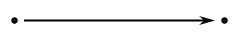
\includegraphics[width=0.8\linewidth]{figures/intro/scg/arcs/const/scg_const_perm_positive2.png}} & \parbox[|c]{2cm}{\centering\ni} & \parbox[|m]{2cm}{\centering\in} & \parbox[|c]{2cm}{\centering->} & \parbox[|m|]{2cm}{\centering<-} ~\\
            % 	\hline
            	
            % 	\parbox[m|]{4.6cm}{\textit{~\\ константная постоянная негативная sc-дуга принадлежности ~\\}} & \parbox[m|]{3.5cm}{\centering 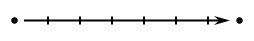
\includegraphics[width=0.8\linewidth]{figures/intro/scg/arcs/const/scg_const_perm_negative2.png}} & \parbox[m]{2cm}{\centering \not\ni} & \parbox[m|]{2cm}{\centering\notin} & \parbox[m|]{2cm}{\centering-|>} & \parbox[m]{2cm}{\centering<|-} ~\\
            % 	\hline
            	
            % 	\parbox[m]{4.6cm}{\textit{~\\ константная постоянная нечеткая sc-дуга принадлежности ~\\}} & \parbox[m]{3.5cm}{\centering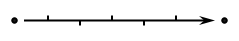
\includegraphics[width=0.8\linewidth]{figures/intro/scg/arcs/const/scg_const_perm_fuzzy2.png}} & \parbox[m]{2cm}{\centering / \ni} & \parbox[m]{2cm}{\centering \in /} & \parbox[m]{2cm}{\centering -/>} & \parbox[m]{2cm}{\centering </-} ~\\
            % 	\hline
            	
            % 	\parbox[m]{4.6cm}{\textit{~\\ константная временная позитивная sc-дуга принадлежности ~\\}} & \parbox[m]{3.5cm}{\centering 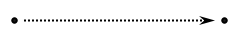
\includegraphics[width=0.8\linewidth]{figures/intro/scg/arcs/const/scg_const_temp_positive2.png}} & \parbox[m]{2cm}{\centering \sim \ni} & \parbox[m]{2cm}{\centering \in \sim} & \parbox[m]{2cm}{\centering \sim>} & \parbox[m]{2cm}{\centering <\sim} ~\\
            % 	\hline
            	
            % 	\parbox[m]{4.6cm}{\textit{~\\ константная временная негативная sc-дуга принадлежности ~\\}} & \parbox[m]{3.5cm}{\centering 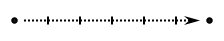
\includegraphics[width=0.8\linewidth]{figures/intro/scg/arcs/const/scg_const_temp_negative2.png}} & \parbox[m]{2cm}{\centering \sim \not\ni} & \parbox[m]{2cm}{\centering \notin \sim} & \parbox[m]{2cm}{\centering \sim|>} & \parbox[m]{2cm}{\centering <|\sim} ~\\
            % 	\hline
            	
            % 	\parbox[m]{4.6cm}{\textit{~\\ константная временная нечеткая sc-дуга принадлежности ~\\}} & \parbox[m]{3.5cm}{\centering 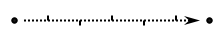
\includegraphics[width=0.8\linewidth]{figures/intro/scg/arcs/const/scg_const_temp_fuzzy2.png}} & \parbox[m]{2cm}{\centering \sim / \ni}  & \parbox[m]{2cm}{\centering \in/\sim} & \parbox[m]{2cm}{\centering \sim/>} & \parbox[m]{2cm}{\centering </\sim} ~\\
            % 	\hline
            	
            % 	\parbox[m]{4.6cm}{\textit{~\\ переменная постоянная позитивная sc-дуга принадлежности ~\\}} & \parbox[m]{3.5cm}{\centering 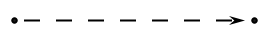
\includegraphics[width=0.8\linewidth]{figures/intro/scg/arcs/var/scg_var_perm_positive2.png}} & \parbox[m]{2cm}{\centering \textunderscore \ni} & \parbox[m]{2cm}{\centering \textunderscore \in} & \parbox[m]{2cm}{\centering \textunderscore->} & \parbox[m]{2cm}{\centering <-\textunderscore} ~\\
            % 	\hline
            	
            % 	\parbox[m]{4.6cm}{\textit{~\\ переменная постоянная негативная sc-дуга принадлежности ~\\}} & \parbox[m]{3.5cm}{\centering 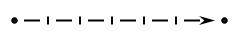
\includegraphics[width=0.8\linewidth]{figures/intro/scg/arcs/var/scg_var_perm_negative2.png}} & \parbox[m]{2cm}{\centering \textunderscore \not\ni} & \parbox[m]{2cm}{\centering \notin \textunderscore} & \parbox[m]{2cm}{\centering \textunderscore-|>} & \parbox[m]{2cm}{\centering <|-\textunderscore} ~\\
            % 	\hline
            	
            % 	\parbox[m]{4.6cm}{\textit{~\\ переменная постоянная нечеткая sc-дуга принадлежности ~\\}} & \parbox[m]{3.5cm}{\centering 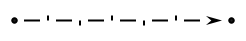
\includegraphics[width=0.8\linewidth]{figures/intro/scg/arcs/var/scg_var_perm_fuzzy2.png}} & \parbox[m]{2cm}{\centering \textunderscore /\ni} & \parbox[m]{2cm}{\centering \in/\textunderscore} & \parbox[m]{2cm}{\centering \textunderscore-/>} & \parbox[m]{2cm}{\centering </-\textunderscore} ~\\
            % 	\hline
            	
            % 	\parbox[m]{4.6cm}{\textit{~\\ переменная временная позитивная sc-дуга принадлежности ~\\}} & \parbox[m]{3.5cm}{\centering 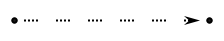
\includegraphics[width=0.8\linewidth]{figures/intro/scg/arcs/var/scg_var_temp_positive2.png}} & \parbox[m]{2cm}{\centering \textunderscore \sim \ni} & \parbox[m]{2cm}{\centering \in \sim \textunderscore} & \parbox[m]{2cm}{\centering \textunderscore \sim >} & \parbox[m]{2cm}{\centering < \sim \textunderscore} ~\\
            % 	\hline
            	
            % 	\parbox[m]{4.6cm}{\textit{~\\ переменная временная негативная sc-дуга принадлежности ~\\}} & \parbox[m]{3.5cm}{\centering 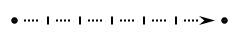
\includegraphics[width=0.8\linewidth]{figures/intro/scg/arcs/var/scg_var_temp_negative2.png}} & \parbox[m]{2cm}{\centering \textunderscore \sim \not$\ni$} & \parbox[c]{2cm}{\centering \notin \sim \textunderscore} & \parbox[m]{2cm}{\centering \textunderscore \sim |>} & \parbox[m]{2cm}{\centering <| \sim \textunderscore} ~\\
            % 	\hline
            	
            % 	\parbox[m]{4.6cm}{\textit{~\\переменная временная нечеткая sc-дуга принадлежности~\\}} & \parbox[m]{3.5cm}{\centering 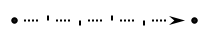
\includegraphics[width=0.8\linewidth]{figures/intro/scg/arcs/var/scg_var_temp_fuzzy2.png}} & \parbox[m]{2cm}{\centering \textunderscore \sim / \ni} & \parbox[m]{2cm}{\centering \in/\sim\textunderscore} & \parbox[m]{2cm}{\centering \textunderscore \sim />} & \parbox[m]{2cm}{\centering </\sim \textunderscore} ~\\
            % 	\hline
            	
            % 	\parbox[m]{4.6cm}{\textit{~\\метапеременная постоянная позитивная sc-дуга принадлежности~\\}} & \parbox[m]{3.5cm}{\centering 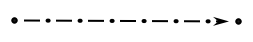
\includegraphics[width=0.8\linewidth]{figures/intro/scg/arcs/meta/scg_metavar_perm_positive2.png}} & \parbox[m]{2cm}{\centering\textunderscore \textunderscore\ni} & \parbox[m]{2cm}{\centering\in\textunderscore\textunderscore} & \parbox[m]{2cm}{\centering\textunderscore\textunderscore->} & \parbox[m]{2cm}{\centering <-\textunderscore\textunderscore} ~\\
            % 	\hline
            	
            % 	\parbox[m]{4.6cm}{\textit{~\\ метапеременная постоянная негативная sc-дуга принадлежности ~\\}} & \parbox[m]{3.5cm}{\centering 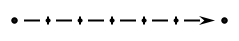
\includegraphics[width=0.8\linewidth]{figures/intro/scg/arcs/meta/scg_metavar_perm_negative2.png}} & \parbox[m]{2cm}{\centering \textunderscore\textunderscore \not\ni} & \parbox[m]{2cm}{\centering \notin\textunderscore\textunderscore} & \parbox[m]{2cm}{\centering \textunderscore\textunderscore-|>} & \parbox[m]{2cm}{\centering <|-\textunderscore\textunderscore} ~\\
            % 	\hline
            	
            % 	\parbox[m]{4.6cm}{\textit{~\\ метапеременная постоянная нечеткая sc-дуга принадлежности ~\\}} & \parbox[m]{3.5cm}{\centering 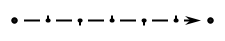
\includegraphics[width=0.8\linewidth]{figures/intro/scg/arcs/meta/scg_metavar_perm_fuzzy2.png}} & \parbox[m]{2cm}{\centering\textunderscore\textunderscore/\ni} & \parbox[m]{2cm}{\centering\in/\textunderscore\textunderscore} & \parbox[m]{2cm}{\centering\textunderscore\textunderscore-/>} & \parbox[m]{2cm}{\centering </-\textunderscore\textunderscore} ~\\
            % 	\hline
            	
            % 	\parbox[m]{4.6cm}{\textit{~\\ метапеременная временная позитивная sc-дуга принадлежности ~\\}} & \parbox[m]{3.5cm}{\centering 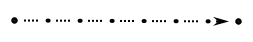
\includegraphics[width=0.8\linewidth]{figures/intro/scg/arcs/meta/scg_metavar_temp_positive2.png}} & \parbox[m]{2cm}{\centering\textunderscore\textunderscore\sim\ni} & \parbox[m]{2cm}{\centering\in\sim\textunderscore\textunderscore} & \parbox[m]{2cm}{\centering\textunderscore\textunderscore\sim>} & \parbox[m]{2cm}{\centering <\sim\textunderscore\textunderscore} ~\\
            % 	\hline
            	
            % 	\parbox[m]{4.6cm}{\textit{~\\ метапеременная временная негативная sc-дуга принадлежности ~\\}} & \parbox[m]{3.5cm}{\centering 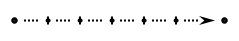
\includegraphics[width=0.8\linewidth]{figures/intro/scg/arcs/meta/scg_metavar_temp_negative2.png}} & \parbox[m]{2cm}{\centering \textunderscore\textunderscore\sim \not\ni} & \parbox[m]{2cm}{\centering\notin\sim\textunderscore\textunderscore} & \parbox[m]{2cm}{\centering\textunderscore\textunderscore\sim|>} & \parbox[m]{2cm}{\centering <|\sim\textunderscore\textunderscore} ~\\
            % 	\hline
            	
            % 	\parbox[m]{4.6cm}{\textit{~\\ метапеременная временная нечеткая sc-дуга принадлежности ~\\}} & \parbox[m]{3.5cm}{\centering 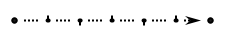
\includegraphics[width=0.8\linewidth]{figures/intro/scg/arcs/meta/scg_metavar_temp_fuzzy2.png}} & \parbox[m]{2cm}{\centering \textunderscore\textunderscore\sim/\ni} & \parbox[m]{2cm}{\centering\in/\sim\textunderscore\textunderscore} & \parbox[m]{2cm}{\centering\textunderscore\textunderscore\sim/>} & \parbox[m]{2cm}{\centering</\sim\textunderscore\textunderscore} ~\\
            % 	\hline
            % \end{longtable}
            % }
            % \scnheader{Таблица. Алфавит sc.s-коннекторов, соответствующих sc.g-коннекторам, которые не являются sc.g-дугами принадлежности}
            % \scneqtable{
            % \begin{longtable}[l]{|m{6.2cm}|m{2.5cm}|m{2.5cm}|m{2.5cm}|m{2.5cm}|}
            %     \hline
            %     \multicolumn{1}{|c}{\parbox[c]{6.2cm}{Изображение \textit{\mbox{sc-коннектора}} в SCg}} &
            %     \multicolumn{2}{|c}{\parbox[c]{5cm}{Изображение \textit{\mbox{sc.s-коннектора}} в Расширенном алфавите}} &
            %     \multicolumn{2}{|c|}{\parbox[c]{5cm}{Изображение \textit{\mbox{sc.s-коннектора}} в Базовом алфавите}}
            %     \hline
            %     \endhead
                
            %     \parbox[|c]{6.2cm}{~\\\centering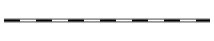
\includegraphics[width=0.8\linewidth]{figures/intro/scs/sc.s-connectors/noorient.png}~\\} & \multicolumn{2}{c|}{ \parbox[c]{5cm}{\centering\leftrightarrow}} & \multicolumn{2}{c|}{ \parbox[c]{5cm}{\centering<>}} ~\\
            %     \hline
                
            %     \parbox[c]{6.2cm}{~\\\centering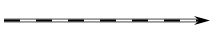
\includegraphics[width=0.8\linewidth]{figures/intro/scs/sc.s-connectors/orient.png} ~\\} &\parbox[c]{2.5cm}{~\\\centering\rightarrow~\\} & \parbox[c]{2.5cm}{~\\\centering\leftarrow~\\} & \parbox[c]{2.5cm}{~\\\centering >>~\\} & \parbox[c|]{2.5cm}{~\\\centering <<~\\} ~\\
            %     \hline
                
            %     \parbox[c]{6.2cm}{~\\\centering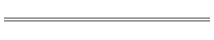
\includegraphics[width=0.8\linewidth]{figures/intro/scs/sc.s-connectors/constPermNoorien.png}~\\} & \multicolumn{2}{c|}{\parbox[c]{5cm}{\centering\Leftrightarrow}} & \multicolumn{2}{c|}{\parbox[c]{5cm}{\centering<=>}} ~\\
            %     \hline
                
            %     \parbox[c]{6.2cm}{~\\\centering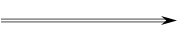
\includegraphics[width=0.8\linewidth]{figures/intro/scs/sc.s-connectors/constPermOrient.png}~\\} & \parbox[c]{2.5cm}{\centering\Rightarrow} & \parbox[c]{2.5cm}{\centering\Leftarrow} & \parbox[c]{2.5cm}{\centering =>} & \parbox[c|]{2.5cm}{\centering <=} ~\\
            %     \hline
                
            %     \parbox[c]{6.2cm}{~\\\centering
\includegraphics[width=0.8\linewidth]{figures/intro/scs/sc.s-connectors/constTempNoorien.png}~\\} & \multicolumn{2}{c|}{\parbox[c]{5cm}{\centering\sim\Leftrightarrow}} & \multicolumn{2}{c|}{\parbox[c|]{5cm}{\centering\sim<=>}} ~\\
            %     \hline
                
            %     \parbox[c]{6.2cm}{~\\\centering 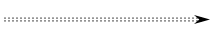
\includegraphics[width=0.8\linewidth]{figures/intro/scs/sc.s-connectors/constTempOrient.png}~\\} & \parbox[c]{2.5cm}{\centering\sim\Rightarrow} & \parbox[c]{2.5cm}{\centering\Leftarrow\sim} & \parbox[c]{2.5cm}{\centering\sim=>} & \parbox[c|]{2.5cm}{\centering <=\sim} ~\\
            %     \hline
                
            %     \parbox[c]{6.2cm}{~\\\centering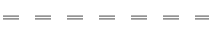
\includegraphics[width=0.8\linewidth]{figures/intro/scs/sc.s-connectors/varPermNoorien.png}~\\} & \multicolumn{2}{c|}{\parbox[c]{5cm}{\centering\textunderscore\Leftrightarrow}} & \multicolumn{2}{c|}{\parbox[c|]{5cm}{\centering\textunderscore<=>}} ~\\
            %     \hline
                
            %     \parbox[c]{6.2cm}{~\\\centering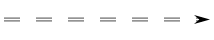
\includegraphics[width=0.8\linewidth]{figures/intro/scs/sc.s-connectors/varPermOrient.png}~\\} & \parbox[c]{2.5cm}{\centering\textunderscore\Rightarrow} & \parbox[c]{2.5cm}{\centering\Leftarrow\textunderscore} & \parbox[c]{2.5cm}{\centering\textunderscore=>} & \parbox[c|]{2.5cm}{\centering <=\textunderscore} ~\\
            %     \hline
                
            %     \parbox[c]{6.2cm}{~\\\centering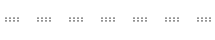
\includegraphics[width=0.8\linewidth]{figures/intro/scs/sc.s-connectors/varTempNoorien.png}~\\} & \multicolumn{2}{c|}{\parbox[c]{5cm}{\centering\textunderscore\sim\Leftrightarrow}} & \multicolumn{2}{c|}{\parbox[c]{5cm}{\centering\textunderscore\sim<=>}} ~\\
            %     \hline
                
            %     \parbox[c]{6.2cm}{~\\\centering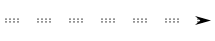
\includegraphics[width=0.8\linewidth]{figures/intro/scs/sc.s-connectors/varTempOrient.png}~\\} & \parbox[c]{2.5cm}{\centering\textunderscore\sim\Rightarrow} & \parbox[c]{2.5cm}{\centering\Leftarrow\sim\textunderscore} & \parbox[c]{2.5cm}{\centering\textunderscore\sim=>} & \parbox[c|]{2.5cm}{\centering <=\sim\textunderscore} ~\\
            %     \hline
                
            %     \parbox[c]{6.2cm}{~\\\centering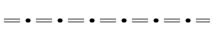
\includegraphics[width=0.8\linewidth]{figures/intro/scs/sc.s-connectors/metaPermNoorien.png}~\\} & \multicolumn{2}{c|}{\parbox[c]{5cm}{\centering\textunderscore\textunderscore\Leftrightarrow}} & \multicolumn{2}{c|}{\parbox[c|]{5cm}{\centering\textunderscore\textunderscore<=>}} ~\\
            %     \hline
                
            %     \parbox[c]{6.2cm}{~\\\centering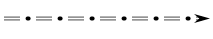
\includegraphics[width=0.8\linewidth]{figures/intro/scs/sc.s-connectors/metaPermOrient.png}~\\} & \parbox[c]{2.5cm}{\centering\textunderscore\textunderscore\Rightarrow} & \parbox[c]{2.5cm}{\centering\Leftarrow\textunderscore\textunderscore} & \parbox[c]{2.5cm}{\centering\textunderscore\textunderscore=>} & \parbox[c|]{2.5cm}{\centering <=\textunderscore\textunderscore} ~\\
            %     \hline
                
            %     \parbox[c]{6.2cm}{~\\\centering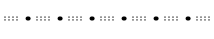
\includegraphics[width=0.8\linewidth]{figures/intro/scs/sc.s-connectors/metaTempNoorien.png}~\\} & \multicolumn{2}{c|}{\parbox[c]{5cm}{\centering\textunderscore\textunderscore\sim\Leftrightarrow}} & \multicolumn{2}{c|}{\parbox[c]{5cm}{\centering\textunderscore\textunderscore\sim<=>}} ~\\
            %     \hline
                
            %     \parbox[c]{6.2cm}{~\\\centering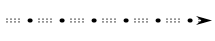
\includegraphics[width=0.8\linewidth]{figures/intro/scs/sc.s-connectors/metaTempOrient.png}~\\} & \parbox[c]{2.5cm}{\centering\textunderscore\textunderscore\sim\Rightarrow} & \parbox[c]{2.5cm}{\centering\Leftarrow\sim\textunderscore\textunderscore} & \parbox[c]{2.5cm}{\centering\textunderscore\textunderscore\sim\Rightarrow} & \parbox[c|]{2.5cm}{\centering\Leftarrow\sim\textunderscore\textunderscore} ~\\
            %     \hline
                
            %     \parbox[c]{6.2cm}{~\\\centering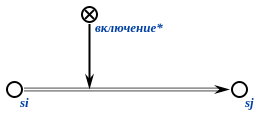
\includegraphics[width=0.8\linewidth]{figures/intro/scs/sc.s-connectors/examples/scs_transf_inclusion_const.png}~\\} & \parbox[c]{2.5cm}{\centering\supseteq} & \parbox[c]{2.5cm}{\centering\subseteq} & \multicolumn{2}{c|}{\parbox[c]{5cm}{}} ~\\
            %     \hline
                
            %     \parbox[c]{6.2cm}{~\\\centering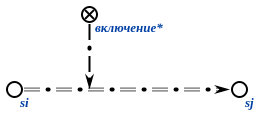
\includegraphics[width=0.8\linewidth]{figures/intro/scs/sc.s-connectors/examples/scs_transf_inclusion_meta.png}~\\} & \parbox[c]{2.5cm}{\centering\textunderscore\supseteq} & \parbox[c]{2.5cm}{\centering\subseteq\textunderscore} & \multicolumn{2}{c|}{\parbox[c|]{5cm}{\centering}} ~\\
            %     \hline
                
            %     \parbox[c]{6.2cm}{~\\\centering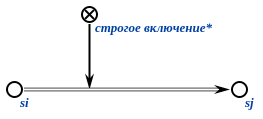
\includegraphics[width=0.8\linewidth]{figures/intro/scs/sc.s-connectors/examples/scs_transf_strict_inclusion_const.png}~\\} & \parbox[c]{2.5cm}{\centering\supset} & \parbox[c]{2.5cm}{\centering\subset} & \multicolumn{2}{c|}{\parbox[c|]{5cm}{}} ~\\
            %     \hline
                
            %     \parbox[c]{6.2cm}{~\\\centering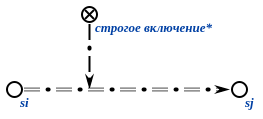
\includegraphics[width=0.8\linewidth]{figures/intro/scs/sc.s-connectors/examples/scs_transf_strict_inclusion_meta.png}~\\} & \parbox[c]{2.5cm}{\centering\textunderscore\supset} & \parbox[c]{2.5cm}{\centering\subset\textunderscore} & \multicolumn{2}{c|}{\parbox[c|]{5cm}{}} ~\\
            %     \hline
                
            %     \parbox[c]{6.2cm}{~\\\centering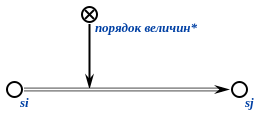
\includegraphics[width=0.8\linewidth]{figures/intro/scs/sc.s-connectors/examples/scs_transf_value_order_const.png}~\\} & \parbox[c]{2.5cm}{\centering\geq} & \parbox[c]{2.5cm}{\centering\leq} & \multicolumn{2}{c|}{\parbox[c|]{5cm}{}} ~\\
            %     \hline
                
            %     \parbox[c]{6.2cm}{~\\\centering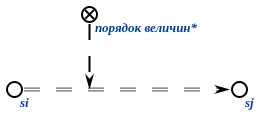
\includegraphics[width=0.8\linewidth]{figures/intro/scs/sc.s-connectors/examples/scs_transf_value_order_var.png}~\\} & \parbox[c]{2.5cm}{\centering\textunderscore\geq} & \parbox[c]{2.5cm}{\centering\textunderscore\leq} & \multicolumn{2}{c|}{\parbox[c]{5cm}{}}  ~\\
            %     \hline
                
            %     \parbox[c]{6.2cm}{~\\\centering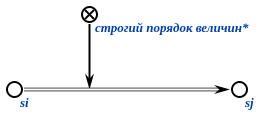
\includegraphics[width=0.8\linewidth]{figures/intro/scs/sc.s-connectors/examples/scs_transf_value_strict_order_const.png}~\\} & \parbox[c]{2.5cm}{\centering >} & \parbox[c]{2.5cm}{\centering <} & \multicolumn{2}{c|}{\parbox[c]{5cm}{}} ~\\
            %     \hline
                
            %     \parbox[c]{6.2cm}{~\\\centering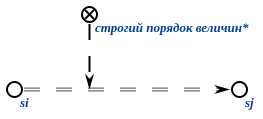
\includegraphics[width=0.8\linewidth]{figures/intro/scs/sc.s-connectors/examples/scs_transf_value_strict_order_var.png}~\\} & \parbox[c]{2.5cm}{\centering\textunderscore>} & \parbox[c]{2.5cm}{\centering <\textunderscore} & \multicolumn{2}{c|}{\parbox[c]{5cm}{}} ~\\
            %     \hline
                
            %     \parbox[c]{6.2cm}{~\\\centering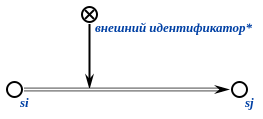
\includegraphics[width=0.8\linewidth]{figures/intro/scs/sc.s-connectors/examples/scs_transf_external_idtf_const.png}~\\} & \multicolumn{2}{c|}{\parbox[c]{5cm}{\centering :=}} & \multicolumn{2}{c|}{\parbox[c]{5cm}{}} ~\\
            %     \hline
                
            %     \parbox[c]{6.2cm}{~\\\centering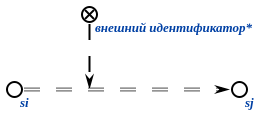
\includegraphics[width=0.8\linewidth]{figures/intro/scs/sc.s-connectors/examples/scs_transf_external_idtf_var.png}~\\} & \multicolumn{2}{c|}{\parbox[c]{5cm}{\centering\textunderscore:=}} & \multicolumn{2}{c|}{\parbox[c]{5cm}{}} ~\\
            %     \hline
                
            %     \parbox[c]{6.2cm}{~\\\centering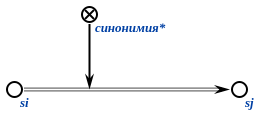
\includegraphics[width=0.8\linewidth]{figures/intro/scs/sc.s-connectors/examples/scs_transf_synonymy_const.png}~\\} & \multicolumn{2}{c|}{\parbox[c]{5cm}{\centering =}} & \multicolumn{2}{c|}{\parbox[c]{5cm}{}} ~\\
            %     \hline
                
            %     \parbox[c]{6.2cm}{~\\\centering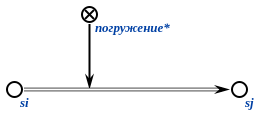
\includegraphics[width=0.8\linewidth]{figures/intro/scs/sc.s-connectors/examples/scs_transf_insertion_const.png}~\\} & \parbox[c]{2.5cm}{\centering\supset=} & \parbox[c]{2.5cm}{\centering = \subset} &  \multicolumn{2}{c|}{\parbox[c]{5cm}{}}  ~\\
            %     \hline
            % \end{longtable}
            % }
            \bigskip
        \end{scnsubstruct}
        \scnendsegmentcomment
        
        \scnsegmentheader{Описание sc.s-предложений}
        \begin{scnsubstruct}
            \scnheader{sc.s-предложение}
            \scnidtf{минимальный семантически целостный фрагмент sc.s-текста}
            \scnidtf{минимальный sc.s-текст}
            \scnsubset{sc.s-текст}
            \scnsuperset{простое sc.s-предложение~\\\scnidtf{минимальное sc.s-предложение}
            \scntext{пояснение}{\textit{sc.s-предложение}, (1) \uline{состоящее} или из двух \textit{sc-идентификаторов}, соединенных между собой \textit{\mbox{sc.s-коннектором}}, или из трех \textit{sc-идентификаторов}, разделенных \textit{sc.s-разделителями, изображающими связь инцидентности sc-элементов}, и (2) завершающееся \textit{двойной точкой с запятой}}\scntext{примечание}{Нетрудно заметить, что простые sc.s-предложения по сути аналогичны триплетам языка RDF (\mbox{RDF-триплетам}), за тем исключением, что \textit{простое sc.s-предложение} можно развернуть\ при помощи \textit{Операции конверсии sc.s-предложений*} не меняя при этом его смысл, а RDF-триплет нельзя. Это является одной из причин, по которой, в отличие от RDF-триплетов, в простых \mbox{sc.s-предложениях} \textit{\mbox{sc.s-коннекторы}} и \textit{\mbox{sc.s-разделители}, изображающие связь инцидентности \mbox{sc-элементов}} не могут быть опущены, поскольку они в том числе показывают направление изображаемой ими связи между sc-элементами.}
            \begin{scnrelfromlist}{пример}
                \scnitem{\scnfileitem{\textit{многоугольник} $\supset$ \textit{треугольник}}\scnrelboth{семантическая эквивалентность}{\scnfileimage[20em]{figures/intro/scs/inclusion.png}}}
                \scnitem{\scnfileitem{\textit{сторона*} $\ni$ (\textit{Четырехугк(ТчкА\char59ТчкВ\char59ТчкС\char59ТчкD)} $\Rightarrow$ \textit{Отр(ТчкВ\char59ТчкС)})\char59\char59}\scnrelboth{семантическая эквивалентность}{\scnfileimage[20em]{figures/intro/scs/side.png}}}
                \scnitem{\scnfileitem{\textit{Si} |- \textit{ai} >| \textit{ei}}\scnrelboth{семантическая эквивалентность}{\scnfileimage[20em]{figures/intro/scs/inclusion_incident.png}}}
            \end{scnrelfromlist}
            }
            \scntext{примечание}{Признаком завершения любого \textit{sc.s-предложения}, т.е. последними его символами является \textit{двойная точка с запятой}, которую, следовательно, можно считать разделителем \textit{sc.s-предложений}.}
            \begin{scnrelfromlist}{заданная операция}
                \scnitem{Операция конверсии sc.s-предложения*~\\\scnsubset{синтаксическая трансформация*}\scntext{пояснение}{Каждое \textit{sc.s-предложение} (в том числе, и \textit{простое sc.s-предложение}) можно преобразовать в семантически эквивалентное ему \textit{sc.s-предложение} путем конверсии (разворота) цепочки компонентов \textit{sc.s-предложения}. Так, например, при конверсии (развороте) простого \textit{\mbox{sc.s-предложения}} (1) первый его \textit{\mbox{sc-идентификатор}} (первый компонент этого \textit{\mbox{sc.s-предложения}}) становится третьим компонентом конвертированного\textit{ \mbox{sc.s-предложения}}, (2) второй его \textit{\mbox{sc-идентификатор}} (третий компонент исходного \textit{\mbox{sc.s-предложения}}) становится первым компонентом конвертированного\ \textit{\mbox{sc.s-предложения}} и (3) второй компонент исходного \textit{\mbox{sc.s-предложения}} (\textit{\mbox{sc.s-коннектор}} или \textit{\mbox{sc.s-разделитель}, изображающий связь инцидентности \mbox{sc-элементов}}, соединяющий указанные выше компоненты) остается вторым компонентом конвертированного \textit{\mbox{sc.s-предложения}}, но меняет направленность ($\ni$\ заменяется на $\in$\ и наоборот, $\supset$\ на $\subset$\ и наоборот, $\Rightarrow$\ на $\Leftarrow$\ и наоборот и т.д.)}\scntext{примечание}{Можно говорить не только о конверсии sc.s-предложения, но и о конверсии sc.s-коннектора, о конверсии sc.s-разделителя, изображающего связь инцидентности sc.s-элементов.}\scnrelfrom{sc.s-текст до трансформации}{\scnfilelong{\textit{треугольник $\ni$ Треуг(ТчкВ\char59ТчкС\char59ТчкD)}\char59\char59}}\scnrelfrom{sc.s-текст после трансформации}{\scnfilelong{\textit{Треуг(ТчкВ\char59ТчкС\char59ТчкD) $\in$ треугольник}\char59\char59}}\scnrelboth{семантическая эквивалентность}{\scnfileimage[20em]{figures/intro/scs/conversion.png}}}
                \scnitem{Операция присоединения sc.s-предложения*~\\\scnsubset{синтаксическая трансформация*}
                \scnidtf{Операция соединения двух sc.s-предложений при совпадении последнего компонента первого предложения с первым компонентом второго*}
                \scntext{пояснение}{В результате выполнения данной операции:
                \begin{scnitemize}
                    \item{первый компонент второго sc.s-предложения удаляется\char59}
                    \item{оставшаяся часть второго предложения окружается sc.s-ограничителем присоединенных предложений ((*\ и *)). Разделитель sc.s-предложений (;;) также попадает внутрь указанного ограничителя\char59}
                    \item{полученная конструкция помещается между последним компонентом первого предложения и разделителем sc.s-предложений, которым заканчивалось первое предложение\char59}
                    \item{второе предложение, таким образом, становится присоединенным sc.s-предложением.}
                \end{scnitemize}
                Аналогичным образом к любому присоединенному sc.s-предложению могут пристыковываться\ другие присоединенные sc.s-предложения, в общем случае уровень такой вложенности не ограничен.}}
                \scnitem{Операция слияния sc.s-предложений*~\\\scnsubset{синтаксическая трансформация*}
                \scnidtf{Операция присоединения простого sc.s-предложения к sc.s-предложению, у которого последний sc.s-коннектор совпадает с sc.s-коннектором простого sc.s-предложения, а предшествующий указанному sc.s-коннектору sc-идентификатор совпадает с первым sc-идентификатором простого sc.s-предложения*}
                \scntext{пояснение}{В результате выполнения этой операции совпадающие sc-идентификаторы и sc.s-коннекторы соединяемых sc.s-предложений склеиваются\ , а последние sc-иден\-ти\-фи\-ка\-то\-ры соединяемых \textit{sc.s-предложений} становятся последними компонентами объединенного \textit{sc.s-предложения},разделенными \textit{точкой с запятой}. Аналогичным образом можно присоединять сколько угодно простых \textit{sc.s-предложений}.}}
                \scnitem{Операция разложения sc.s-предложений на простые sc.s-предложения*~\\\scnsubset{синтаксическая трансформация*}
                \scntext{пояснение}{Каждое \textit{sc.s-предложение} можно разложить на множество \textit{простых sc.s-предложений}, т.е. представить в виде последовательности \textit{простых sc.s-предложений}.}}
                \scnitem{Операция разложения sc.s-предложений на простые sc.s-предложения с sc.s-разделителем, изображающим связь инцидентности sc-элементов*~\\\scnsubset{синтаксическая трансформация*}
                \scntext{пояснение}{Каждое \textit{sc.s-предложение} (в том числе и \textit{простое sc.s-предложение} с \textit{sc.s-коннектором}) можно представить в виде семантически эквивалентной последовательности \textit{простых \mbox{sc.s-предложений}} с \textit{sc.s-разделителем, изображающим связь инцидентности \mbox{sc-элементов}}.}\scntext{примечание}{Данная операция осуществляет \uline{однозначное} (!) формирование множества \textit{простых \mbox{sc.s-предложений}} указанного вида.}}
            \end{scnrelfromlist}
            \newpage\scnheader{sc.s-предложение}
            \scntext{примечание}{Операции, заданные на множестве \textit{sc.s-предложений} можно разделить на три группы:
            \begin{scnitemize}
                \item{группа операций конверсии \textit{sc.s-предложений}, состоящая из одной операции;}
                \item{группа операций соединения \textit{sc.s-предложений};}
                \item{группа операций декомпозиции \textit{sc.s-предложений} и, в частности, операций разложения \textit{sc.s-предложений}.}
            \end{scnitemize}
            Очевидно, что операции соединения \textit{sc.s-предложений} и операции декомпозиции \textit{sc.s-предложений} являются обратными друг другу операциями.}\scnheader{Описание примеров выполнения операций, заданных на множестве sc.s-предложений}
            \begin{scnsubstruct}
            \bigskip\scnfilelong{\textit{треугольник $\ni$ Треугк(ТчкВ\char59ТчкС\char59ТчкD)}\char59\char59}
            \scnrelfrom{Операция конверсии sc.s-предложения}{\scnfilelong{\textit{Треугк(ТчкВ\char59ТчкС\char59ТчкD) $\in$ треугольник}\char59\char59}}
            \scnrelboth{семантическая эквивалентность}{\scnfileimage[20em]{figures/intro/scs/conversion.png}}
            \bigskip\bigskip{\scnfilelong{\textit{треугольник $\ni$ Треугк(ТчкВ\char59ТчкС\char59ТчкD)\char59\char59\newlineТреугк(ТчкВ\char59ТчкС\char59ТчкD) $\Rightarrow$ сторона*:включение*: Отр(ТчкВ\char59ТчкC)\char59\char59}}}\scnrelfrom{Операция присоединения sc.s-предложения}{\scnfilelong{\textit{треугольник $\ni$ Треугк(ТчкВ\char59ТчкС\char59ТчкD) (* $\Rightarrow$ сторона*:включение*:Отр(ТчкВ\char59ТчкС)\char59\char59*) }\char59\char59}}
            \scnrelboth{семантическая эквивалентность}{\scnfileimage[20em]{figures/intro/scs/joining_sentences.png}}
            \bigskip\bigskip\scnfilelong{\textit{сторона* $\ni$ (Треугк(ТчкВ\char59Тчк С\char59ТчкD) $\Rightarrow$ Отр(ТчкВ\char59ТчкС))\char59\char59\newlineсторона* $\ni$ (Треугк(ТчкВ\char59Тчк С\char59ТчкD) $\Rightarrow$ Отр(ТчкC\char59ТчкD))\char59\char59}}
            \scnrelfrom{Операция слияния sc.s-предложений}{\scnfilelong{\textit{сторона* $\ni$ ((Треугк(ТчкВ\char59ТчкС\char59ТчкD) $\Rightarrow$ Отр(ТчкВ\char59ТчкС))\char59(Треуг(ТчкВ\char59ТчкС\char59ТчкD) $\Rightarrow$ Отр(ТчкC\char59ТчкD)))\char59\char59}}}
            \scnrelfrom{синтаксическая трансформация}{\scnfilelong{\textit{Треугк(ТчкВ\char59ТчкС\char59ТчкD)}$\Rightarrow$\textit{сторона*}: \textit{Отр(ТчкВ\char59ТчкС)}\char59\textit{Отр(ТчкС\char59ТчкD)}\char59\char59}}
            \scnrelboth{семантическая эквивалентность}{\scnfileimage[20em]{figures/intro/scs/joining_sentence.png}}
            \bigskip\bigskip\newpage{\scnfilelong{\textit{Треугк(ТчкВ\char59ТчкС\char59ТчкD) $\Rightarrow$ сторона*:включение*:Отр(ТчкВ\char59ТчкС)\char59\char59}}}\scnrelfrom{Операция разложения sc.s-предложений на простые sc.s-предложения}{\scnfilelong{\textit{сторона* $\ni$ (Треугк(ТчкВ\char59ТчкС\char59ТчкD) $\Rightarrow$ Отр(ТчкВ\char59ТчкС))\char59\char59\newline включение* $\ni$ (Треугк(ТчкВ\char59ТчкС\char59ТчкD) $\Rightarrow$ Отр(ТчкВ\char59ТчкС))\char59\char59}}}
            \scnrelboth{семантическая эквивалентность}{\scnfileimage[20em]{figures/intro/scs/dividing_sentences.png}}
            \bigskip\bigskip{\scnfilelong{\textit{треугольник $\ni$ Треугк(ТчкВ\char59ТчкC\char59ТчкD)}}}\scnrelfrom{Операция разложения sc.s-предложений на простые sc.s-предложения с sc.s-разделителем, изображающим связь инцидентности sc-элементов}{\scnfilelong{\textit{треугольник |- ai >| Треугк(ТчкВ\char59ТчкС\char59ТчкD)\char59\char59\newlineконстантный постоянный sc-узел, обозначающий класс $\ni$ треугольник\char59\char59\newlineконстантная постоянная позитивная sc-дуга принадлежности $\ni$ ai\char59\char59\newlineконстантный постоянный sc-узел общего вида $\ni$ Треугк(ТчкВ\char59ТчкC\char59ТчкD)\char59\char59}}}
            \scnrelboth{семантическая эквивалентность}{\scnfileimage[20em]{figures/intro/scs/dividing_sentences_incident.png}}
            \scnheader{присоединенное sc.s-предложение}
            \scnidtf{встроенное sc.s-предложение}
            \scntext{пояснение}{Присоединенные sc.s-предложения используются для того, чтобы продолжить спецификацию какого-либо sc-элемента, sc-идентификатор которого является последним компонентом в рамках какого-либо sc.s-предложения, не начиная при этом нового sc.s-предложения и, таким образом, не дублируя указанный \mbox{sc-идентификатор}. Внутрь присоединенных sc.s-предложений также могут встраиваться другие присоединенные sc.s-предложения, в общем случае уровень вложенности таких предложений не ограничен. Таким образом присоединенные sc.s-предложения описывают ветвление\ sc.s-предложений, при этом точками такого ветвления\ выступают sc-идентификаторы, входящие в состав этих sc.s-предложений.Благодаря введению присоединенных sc.s-предложений появляется возможность любой sc-текст изобразить в виде одного sc.s-предложения, содержащего необходимое количество присоединенных sc.s-предложений. Таким образом, SCs-код по выразительной мощности становится эквивалентным SCn-коду.}\scnheader{sc.s-предложение}
            \scntext{денотационная семантика}{С семантической точки зрения \textit{sc.s-предложение} представляет собой описание некоторого \uline{маршрута} в соответствующем sc-тексте, который является графовой структурой специального вида и структура которого описывается (изображается) с помощью \textit{sc.s-предложений}. Указанный маршрут проводится\ по sc-коннекторам и по связям инцидентности sc-элементов, если маршрут проходит через инцидентные sc-коннекторы. В описании указанного маршрута могут дополнительно указываться множества (чаще всего отношения), которым принадлежат sc-коннекторы, входящие в описываемый маршрут. Кроме того, указанный маршрут в начале и/или в конце может иметь разветвления, когда какой-либо sc-элемент \uline{одинаково} инцидентен нескольким \uline{однотипным} sc-коннекторам, соединяющим указанный sc-элемент с некоторыми другими sc-элементами.Таким образом каждое указанное разветвление состоит из неограниченного числа ветвей, каждая из которых состоит из одного sc-коннектора и одного связываемого им sc-элемента.}
            \scnheader{компонент sc.s-предложения*}
            \scntext{пояснение}{Каждое \textit{sc.s-предложение} представляет собой последовательность (1) \textit{sc-идентификаторов}, \mbox{(2) \textit{sc.s-коннекторов}} или \textit{sc.s-разделителей}, изображающих связь инцидентности \textit{sc-элементов}, (3) \textit{точек с запятыми}, (4) \textit{ограничителей присоединенных sc.s-предложений}, завершаемая \textit{двойной точкой с запятой}. При этом непосредственно соседствовать друг с другом не могут ни \textit{\mbox{sc-идентификаторы}}, ни \textit{\mbox{sc.s-коннекторы}}, ни, очевидно, \textit{точки с запятыми} и \textit{ограничители присоединенных sc.s-предложений}.~\\Между \textit{sc-идентификаторами} в рамках \textit{sc.s-предложения} может находиться либо \textit{точка с запятой}, либо \textit{sc.s-коннектор}, либо \textit{sc.s-разделитель}, изображающий связь инцидентности \textit{sc-элементов}. Слева и справа от \textit{sc.s-коннектора} и от \textit{sc.s-разделителя}, изображающего связь инцидентности \textit{sc-элементов}, должны находиться \textit{sc-идентификаторы}.Указанные \textit{sc-идентификаторы}, \textit{sc.s-коннекторы} и \textit{sc.s-разделители}, изображающие связь инцидентности \textit{sc-элементов}, считаются компонентами соответствующего \textit{sc.s-предложения}. Понятие быть компонентом sc.s-предложения\ является относительным понятием (отношением), т.к. в состав некоторых компонентов \textit{sc.s-предложения} (в состав \textit{sc-идентификаторов}, являющихся \textit{sc.s-выражениями}, ограничиваемыми фигурными или квадратными скобками) могут входить других \textit{sc.s-предложения}, состоящие из своих компонентов.}\scnrelfrom{первый домен}{sc.s-предложение}
            \scnrelfrom{второй домен}{{\normalfont (} sc-идентификатор $\cup$ sc.s-разделитель $\cup$ sc.s-ограничитель {\normalfont )}}
            \scnheader{sc.s-модификатор*}
            \scnsubset{компонент sc.s-предложения*}
            \scntext{пояснение}{Это дополнительный вид компонентов \textit{sc.s-предложений}. Каждый \textit{sc.s-модификатор}, являющийся компонентом некоторого \textit{sc.s-предложения}, представляет собой \textit{sc-идентификатор}, обозначающий множество (чаще всего, отношение), которому принадлежит sc-коннектор, изображенный \textit{sc.s-коннектором}, который предшествует указанному \textit{sc-идентификатору}. Признаком \textit{sc.s-модификатора} является \textit{двоеточие} (или \textit{двойное двоеточие}), которое ставится после \textit{sc.s-модификатора} и отделяет его либо от следующего за ним другого \textit{sc.s-модификатора} для этого же \textit{sc.s-коннектора}, либо от следующего за ним \textit{sc-идентификатора}, соответствующего sc-элементу, который инцидентен sc-коннектору, изображенному \textit{sc.s-коннектором}, находящимся левее рассматриваемого \textit{sc-идентификатора} после одного или нескольких \textit{sc.s-модификаторов}. Обычное (одинарное) \textit{двоеточие} обозначает, что sc-элемент, изображенный соответствующим \mbox{sc.s-модификатором}, связан с sc-коннектором, изображенным левее этого \mbox{sc.s-модификатора}, \textit{базовой \mbox{sc-дугой}} (\textit{константной постоянной позитивной \mbox{sc-дугой} принадлежности}), \textit{двойное двоеточие} обозначает, что указанные элементы связаны \textit{переменной постоянной позитивной \mbox{sc-дугой} принадлежности}.}
            \begin{scnrelfromlist}{пример}
                \scnitem{\scnfileitem{\textit{Четырехугк(ТчкА;ТчкВ;ТчкС;ТчкD)} $\Rightarrow$ \textit{сторона*} : \textit{включение*} : \textit{Отр(ТчкВ;ТчкС)};;}
                ~\\\scnrelboth{семантическая эквивалентность}{\scnfileimage[20em]{figures/intro/scs/modifier.png}}
                }
                \scnitem{ \textit{Треугк(ТчкА;ТчкВ;ТчкС)} $\_\Rightarrow$ \textit{сторона*} :: \textit{\_s};; 
                ~\\\scnrelboth{семантическая эквивалентность}{\scnfileimage[20em]{figures/intro/scs/modifier_var.png}}
                }
            \end{scnrelfromlist}
            \scnheader{sc.s-текст}
            \scnidtf{конкатенация \textit{sc.s-предложений}}
            \scnidtf{последовательность \textit{sc.s-предложений}, разделяемых \textit{двойными точками с запятой}}
            \scnsuperset{максимальный исходный sc.s-текст}
            \scnidtf{конкатенция \textit{sc.s-предложений}, слева и справа от которой отсутствуют какие-либо символы SCs-кода}
            \scnsuperset{максимальный sc.s-текст, включенный в структуру}
            \scnidtf{конкатенция всех \textit{sc.s-предложений}, входящих в состав \textit{sc.s-выражения структуры}}
            \scnsuperset{sc.s-текст, включенный в структуру}
            \scnidtf{часть цепочки \textit{sc.s-предложений}, входящих в состав максимального sc.s-текста, включенного в структуру}
            \scnsuperset{sc.s-предложение, включенное в структуру}
            \scntext{примечание}{\textit{sc.s-предложение} является минимальным sc.s-текстом.}\scntext{свойство}{Смысл sc.s-текста (а также \textit{sc.s-текста, включенного в структуру} не зависит от порядка \textit{\mbox{sc.s-предложений}} в этих sc-текстах. Т.е. перестановка \textit{\mbox{sc.s-предложений}} в рамках таких \mbox{sc.s-текстов} смысла этих \mbox{sc.s-текстов} не меняет (т.е. приводит к семантически эквивалентным \mbox{sc.s-текстам}), но сильно влияет на трудоемкость человеческого восприятия (на читабельность) этих текстов.}
            \scnrelfrom{пример}{\scnfilelong{\textit{материальный объект} $\ni$ \textit{Земля} (* => \textit{вращаться вокруг}*: \textit{спутник}*: \textit{Луна};;*);;~\\\textit{материальный объект} $\ni$ \textit{Луна}(* => \textit{основной идентификатор}*: [Moon] (* <- \textit{Английский язык};; *); [Луна] (* <- \textit{Русский язык};; *);; *);;~\\\textit{материальный объект} $\ni$ \textit{Солнце} (* => \textit{вращаться вокруг}*: \textit{Земля}; \textit{Марс};; *);;~\\\textit{материальный объект} $\ni$ \textit{Марс};;}
            }
            \scnrelfrom{семантическая эквивалентность}{ \scnfileimage[20em]{figures/intro/scs/scs_text_example.png}
            }
            \bigskip
        \end{scnsubstruct}
        \scnendsegmentcomment
        
        \scnsegmentheader{Описание Ядра SCs-кода и различных направлений его расширения}
        \begin{scnsubstruct}
            \scnheader{Ядро SCs-кода}
            \scnidtf{Подъязык SCs-кода, который использует минимальный набор синтаксических средств, но при этом имеет семантическую мощность, эквивалентную мощности SCs-кода в целом}
            \scntext{принципы, лежащие в основе}{В Ядре SCs-кода:
            \begin{scnitemize}
                \item{используются только \textit{простые sc-идентификаторы}, в том числе \textit{sc-идентификаторы внешних файлов ostis-систем} (sc-выражения не используются);}
                \item{используются только \textit{sc.s-разделители, изображающие связь инцидентности sc-элементов}, а также sc.s-коннектор, изображающий константную  постоянную позитивную пару принадлежности ($\in$ и $\ni$ в Расширенном алфавите и "{}->{}"\ и "{}<-{}"\ в Базовом алфавите). Другие \textit{sc.s-коннекторы} не используются;}
                \item{не используются \textit{sc.s-модификаторы} и, соответственно, двоеточия, являющиеся признаком завершения \textit{sc.s-модификаторов};}
                \item{используются только \textit{простые sc.s-предложения}, которые, как следует из вышеуказанных свойств Ядра SCs-кода, либо состоят из двух \textit{простых sc-идентификаторов}, соединяемых sc.s-коннектором, изображающим константную  постоянную позитивную пару принадлежности, либо трех \textit{простых sc-идентификаторов}, разделенных \textit{sc.s-разделителями, изображающими связь инцидентности sc-элементов}.}
            \end{scnitemize}
            Из перечисленных свойств Ядра SCs-кода следует, что для представления (изображения) любого \mbox{sc-текста} средствами Ядра SCs-кода необходимо для \uline{всех} (!) sc-элементов этого \mbox{sc-текста} (кроме константных постоянных позитивных пар принадлежности) построить соответствующие им простые \textit{sc-идентификаторы}, т.е. необходимо проименовать все указанные sc-элементы. В свою очередь, тип каждого используемого \mbox{sc-элемента} (кроме константных постоянных позитивных пар принадлежности) задается явно путем указания принадлежности этих элементов соответствующим классам sc-элементов, в том числе классам, входящим в Ядро SC-кода.Как видно из приведенного описания, Ядро SCs-кода соответствует Ядру SCg-кода, за исключением того, что в Ядре SCg-кода нет необходимости именовать все изображаемые sc-элементы, а также в Ядре SCg-кода присутствуют графические изображения для sc-элементов, принадлежащих соответствующим классам Ядра SC-кода и эту принадлежность нет необходимости указывать явно.}
            \scntext{примечание}{Очевидно, что широко практически применять Ядро SCs-кода для записи больших фрагментов баз знаний неудобно и неэффективно. Тем не менее, с практической точки зрения Ядро SCs-кода может использоваться, например, для обмена информацией со сторонними средствами представления графовых конструкций, рассчитанными на представление информации в виде триплетов (например, RDF-хранилищ).Для обеспечения возможности более широкого практического использования необходимы синтаксические расширения Ядра SCs-кода в целях:
            \begin{scnitemize}
                \item{минимизации числа идентифицируемых (именуемых) sc-элементов путем использования \textit{sc-выражений} и ликвидации необходимости идентифицировать (именовать) \uline{все} (!) sc-элементы;}
                \item{сокращения текста путем минимизации числа повторений одного и того же \textit{sc-идентификатора} путем соединения \textit{sc.s-предложений};}
                \item{повышение уровня наглядности, читабельности\ sc.s-текстов.}
            \end{scnitemize}
            }
            \scnhaselementrole{пример}{\scnfilelong{\textit{треугольник |- ai >| Треугк(ТчкВ\char59ТчкС\char59ТчкD)\char59\char59\newlineТреугк(ТчкВ\char59ТчкС\char59ТчкD) |- bi >| Отр(ТчкВ\char59ТчкС)\char59\char59\newlineсторона* |- сi >| bi\char59\char59\newlineконстантный постоянный sc-узел, обозначающий класс $\ni$ треугольник\char59\char59\newlineконстантный постоянный sc-узел, обозначающий отношение $\ni$ сторона*\char59\char59\newlineконстантная постоянная позитивная sc-дуга принадлежности $\ni$ ai\char59\char59\newlineконстантная постоянная sc-дуга $\ni$ bi\char59\char59\newlineконстантная постоянная позитивная sc-дуга принадлежности $\ni$ ci\char59\char59\newlineконстантный постоянный sc-узел общего вида $\ni$ Отр(ТчкВ\char59ТчкС)\char59\char59\newlineконстантный постоянный sc-узел общего вида $\ni$ Треугк(ТчкВ\char59ТчкC\char59ТчкD)\char59\char59}}}
            \bigskip
            \scnrelboth{семантическая эквивалентность}{\scnfileimage[20em]{figures/intro/scs/kernel_incident.png}}
            \scnheader{Первое направление расширения Ядра SCs-кода}
            \scnidtf{Первое направление расширения Ядра SCs-кода \uline{и всех иных его расширений}}
            \scntext{принципы}{По сравнению с \textit{Ядром SCs-кода} в \textit{Первом направлении расширения Ядра SCs-кода} вместо \textit{sc-идентификато|-ров}, являющихся идентификаторами (именами), которые взаимно однозначно соответствуют синонимичным им (представляемым ими) sc-коннекторам, вводятся \textit{sc.s-коннекторы}, каждый из которых соответствует не одному конкретному sc-коннектору, а некоторому классу однотипных sc-коннекторов. Очевидно, что это ликвидирует необходимость \uline{каждому} sc-коннектору приписывать уникальный \textit{sc-идентификатор}. Кроме того, \textit{Алфавит sc.s-коннекторов} включает в себя элементы этого Алфавита (классы \uline{синтаксически} эквивалентных \textit{sc.s-коннекторов}), которые соответствуют \uline{всем} (!) элементам Алфавита sc-коннекторов, но при этом дополнительно включают в себя и другие элементы Алфавита \textit{sc.s-коннекторов}, которые соответствуют часто используемым \uline{семантически} явно выделяемым классам sc-коннекторов. К таким дополнительно вводимым классам \textit{sc.s-коннекторов} относятся \textit{константные sc.s-коннекторы} включения множеств ($\supset$\ или $\subset$), \textit{переменные sc.s-коннекторы} включения множеств ($\_\supset$\ или $\subset\_$), \textit{sc.s-коннектор} синонимии ($=$), \textit{sc.s-коннектор} погружения ($=\subset$\ или $\supset=$) и др.Заметим, что указанное расширение Алфавита \textit{sc.s-коннекторов} аналогично расширенному Алфавиту \textit{sc.g-коннекторов} в SCg-коде и ликвидирует необходимость (как и в SCs-коде) явно специфицировать (средствами SCs-кода) синтаксически выделяемые классы \textit{sc.s-коннекторов}.}
            \scnheader{Второе направление расширения Ядра SCs-кода}
            \scntext{принципы}{Во Втором направлении расширения Ядра SCs-кода вводятся модификаторы \textit{sc.s-коннекторов} (\textit{\mbox{sc.s-модификаторы}}), которые позволяют достаточно компактно дополнительно специфицировать \mbox{sc-коннекторы}, изображаемые (представляемые) соответствующими \textit{sc.s-коннекторами}. Речь идет о такой часто востребованной форме спецификации sc-коннекторов, как указание множества (возможно, нескольких множеств), которому принадлежит специфицируемый  sc-коннектор (чаще всего, таким множеством является \textit{бинарное отношение} (в частности, \textit{ролевое отношение}) или \textit{квазибинарное отношение}).}
            \scnheader{sc.s-модификатор*}
            \scniselement{отношение}
            \scnidtf{относительное понятие}
            \scnidtf{модификатор sc.s-коннектора*}
            \scntext{пояснение}{\textit{sc-идентификатор}, который (1) находится либо между \textit{sc.s-коннектором} и \textit{двоеточием}, либо между \textit{двоеточиями} и (2) обозначает множество (чаще всего, отношение), которому принадлежит sc-коннектор, изображаемый ближайшим предшествующим \textit{sc.s-коннектором}. Два подряд идущих двоеточия (::) обозначают, что указанное множество связано с указанным sc-коннектором \textit{\uline{переменной} позитивной постоянной sc-дугой принадлежности}.Очевидно, что, если не использовать \textit{sc.s-модификаторы}, указанного вида спецификация sc-коннекторов средствами SCs-кода будет выглядеть значительно более громоздкой.}\scnheader{Третье направление расширения Ядра SCs-кода}
            \scntext{принципы}{В \textit{Третьем направлении расширения Ядра SCs-кода} осуществляется переход от использования только \textit{простых sc-идентификаторов} к использованию как \textit{простых sc-идентификаторов}, так и \textit{sc-выражений}, а также к использованию \textit{sc.s-представлений некоторых неидентифицируемых sc-узлов}. Это существенно сокращает число придумываемых \textit{простых sc-идентификаторов}, т.к. каждое \textit{sc-выражение} в конечном счете  это комбинация \textit{простых sc-идентификаторов}, построенная по правилам, которые достаточно легко семантически интерпретируются. Если проводить аналогию с SCg-кодом, то очевидно, что \textit{\mbox{sc-выражение}}, ограничиваемое фигурными скобками, есть не что иное, как информационная конструкция, ограничиваемая \textit{sc.g-контуром}, а \textit{sc-выражение}, ограничиваемое квадратными скобками есть не что иное, как информационная конструкция, ограничиваемая \textit{sc.g-рамкой}. Отличие здесь заключается в том, что круглыми и квадратными скобками можно ограничивать только линейные информационные конструкции (цепочки символов).}
            \scnheader{sc.s-представление неидентифицируемого sc-узла}
            \scnidtf{изображение (представление) неидентифицируемого (неименуемого) sc-узла в sc.s-тексте}
            \scnidtf{sc.s-обозначение неименуемой сущности, не являющейся парой, обозначаемой sc-коннектором}
            \scnidtf{sc.s-представление sc-узла, не являющееся sc-идентификатором (именем этого sc-узла)}
            \begin{scnreltoset}{разбиение}
                \scnitem{sc.s-обозначение неименуемой структуры~\\\scnidtf{конкатенация левой фигурной скобки и правой фигурной скобки}}
                \scnitem{sc.s-обозначение неименуемой неориентированной связки~\\\scnidtf{конкатенация левой фигурной скобки, дефиса и правой фигурной скобки}}
                \scnitem{sc.s-обозначение неименуемого кортежа~\\\scnidtf{конкатенация левой угловой скобки, дефиса и правой угловой скобки}}
                \scnitem{sc.s-обозначение неименуемого файла-экземпляра~\\\scnidtf{конкатенация левой квадратной скобки и правой квадратной скобки}}
                \scnitem{sc.s-обозначение неименуемого файла-класса~\\\scnidtf{конкатенация восклицательного знака, левой квадратной скобки и правой квадратной скобки}}
                \scnitem{sc.s-обозначение неименуемой терминальной сущности~\\\scnidtf{конкатенация левой круглой скобки, буквы о\ и правой круглой скобки}}
            \end{scnreltoset}
            \scntext{примечание}{Если одно и то же обозначение неименуемой сущности встречается в \uline{разных} \textit{sc.s-предложениях}, то считается, что это обозначения \uline{разных} сущностей, т.е. изображения \uline{разных} sc-узлов.}
            \scnheader{Четвертое направление расширения Ядра SCs-кода}
            \scntext{принципы}{В \textit{Четвертом направлении расширения Ядра SCs-кода} осуществляется переход от использования только \textit{простых sc.s-предложений} к использованию также \textit{sc.s-предложений}, построенных с помощью \textit{\mbox{Операции} присоединения sc.s-предложения*}. В результате этого, благодаря склеиванию\ одинаковых \textit{\mbox{sc-идентификаторов}}, а также склеиванию\ синтаксически эквивалентных \textit{\mbox{sc.s-коннекторов}} с одинаковыми \textit{\mbox{sc.s-модификаторами}} (несмотря на то, что эти склеиваемые\ \textit{sc.s-коннекторы} соответствуют \uline{разным} \mbox{sc-коннекторам}), существенно сокращается число копий используемых \textit{\mbox{sc-идентификаторов}} и \textit{\mbox{sc.s-коннекторов}} с их \textit{\mbox{sc.s-модификаторами}}.}
            \newpage\scnheader{Пятое направление расширения Ядра SCs-кода}
            \scntext{принципы}{В \textit{Пятом направлении расширения Ядра SCs-кода} разрешается использование \textit{присоединенных \mbox{sc.s-предложений}}. В результате этого \textit{sc.s-тексты} становятся более компактными и удобными для восприятия за счет снижения числа дублируемых \textit{sc-идентификаторов} и более широких возможностей их структуризации.}
            \scnheader{следует отличать*}
            \begin{scnhaselementset}
                \scnitem{sc.s-представление неидентифицируемого sc-узла}
                \scnitem{sc.s-коннектор~\\\scnidtf{sc.s-представление неидентифицируемого sc-коннектора}}
            \end{scnhaselementset}
            \bigskip
            \begin{scnhaselementset}
                \scnitem{sc-коннектор}
                \scnitem{sc.s-коннектор}
            \end{scnhaselementset}
            \bigskip
            \begin{scnhaselementset}
                \scnitem{sc.s-коннектор}
                \scnitem{sc.s-модификатор*~\\\scnidtf{модификатор sc.s-коннектора*}\scniselement{отношение}}
            \end{scnhaselementset}
            \bigskip
            \begin{scnhaselementset}
                \scnitem{sc.s-коннектор}
                \scnitem{Правила построения sc.s-коннекторов}
            \end{scnhaselementset}
            \bigskip
            \begin{scnhaselementset}
                \scnitem{sc.s-предложение}
                \scnitem{Правила построения sc.s-предложений}
            \end{scnhaselementset}
            \bigskip
            \begin{scnhaselementset}
                \scnitem{sc.s-коннектор}
                \scnitem{sc.g-коннектор}
            \end{scnhaselementset}
            \bigskip\begin{scnhaselementset}
                \scnitem{sc.s-текст}
                \scnitem{sc.g-текст}
            \end{scnhaselementset}
            \scnheader{Примеры sc.s-текстов, трансформируемых по различным направлениям расширений SCs-кода}
\begin{scnset}
    \scnfilelong{\textit{включение* $\ni$ pair1;;\\включение* $\ni$ pair2;;\\включение* $\ni$ pair3;;\\включение* $\ni$ pair4;;\\включение* $\ni$ pair5;;\\сторона* $\ni$ pair1;;\\сторона* $\ni$ pair2;;\\сторона* $\ni$ pair3;;\\сторона* $\ni$ pair4;;\\сторона* $\ni$ pair5;;\\Четырехугк(ТчкА;ТчкВ;ТчкС;ТчкD) |- pair1 >| Отр(ТчкВ;ТчкС);;\\Четырехугк(ТчкА;ТчкВ;ТчкС;ТчкD) |- pair2 >| Отр(ТчкC;ТчкD);;\\Треугк(ТчкВ;ТчкС;ТчкD) |- pair3 >| Отр(ТчкВ;ТчкС);;\\Треугк(ТчкВ;ТчкС;ТчкD) |- pair4 >| Отр(ТчкC;ТчкD);;\\Треугк(ТчкВ;ТчкС;ТчкD) |- pair5 >| Отр(ТчкB;ТчкD);;\\четырехугольник $\ni$ Четырехугк(ТчкА;ТчкВ;ТчкС;ТчкD);;\\треугольник $\ni$ Треугк(ТчкВ;ТчкС;ТчкD);;\\link1 |- pair6 >| Треугк(ТчкВ;ТчкС;ТчкD);;\\декомпозиция фигуры* $\ni$ pair6;;\\link1 $\ni$ Отр(ТчкВ;ТчкС);;\\link1 $\ni$ Отр(ТчкC;ТчкD);;\\link1 $\ni$ Отр(ТчкВ;ТчкD);;}}
    \begin{scnindent}
        \scnrelboth{семантическая эквивалентность}{\scnfileimage[20em]{figures/intro/scs/scs_transf_example.png}}
        \scnrelfrom{синтаксическая трансформация}{\scnfilelong{\textit{сторона* $\ni$ (Четырехугк(ТчкА;ТчкВ;ТчкС;ТчкD) $\Rightarrow$ Отр(ТчкВ;ТчкС));;\\сторона* $\ni$ (Четырехугк(ТчкА;ТчкВ;ТчкС;ТчкD) $\supseteq$ Отр(ТчкC;ТчкD));;\\сторона* $\ni$ (Треугк(ТчкВ;ТчкС;ТчкD) $\supseteq$ Отр(ТчкВ;ТчкС));;\\сторона* $\ni$ (Треугк(ТчкВ;ТчкС;ТчкD) $\supseteq$ Отр(ТчкC;ТчкD));;\\сторона* $\ni$ (Треугк(ТчкВ;ТчкС;ТчкD) $\supseteq$ Отр(ТчкB;ТчкD));;\\Четырехугк(ТчкА;ТчкВ;ТчкС;ТчкD) $\supseteq$ Отр(ТчкВ;ТчкС);;\\Четырехугк(ТчкА;ТчкВ;ТчкС;ТчкD) $\supseteq$ Отр(ТчкC;ТчкD);;\\Треугк(ТчкВ;ТчкС;ТчкD) $\supseteq$ Отр(ТчкВ;ТчкС);;\\Треугк(ТчкВ;ТчкС;ТчкD) $\supseteq$ Отр(ТчкC;ТчкD);;\\Треугк(ТчкВ;ТчкС;ТчкD) $\supseteq$ Отр(ТчкB;ТчкD);;\\четырехугольник $\ni$ Четырехугк(ТчкА;ТчкВ;ТчкС;ТчкD);;\\треугольник $\ni$ Треугк(ТчкВ;ТчкС;ТчкD);;\\декомпозиция фигуры* $\ni$ (link1 $\Rightarrow$ Треугк(ТчкВ;ТчкС;ТчкD));;\\link1 $\ni$ Отр(ТчкВ;ТчкС);;\\link1 $\ni$ Отр(ТчкC;ТчкD);;\\link1 $\ni$ Отр(ТчкВ;ТчкD);;}}}
        \begin{scnindent}
            \scnrelfrom{синтаксическая трансформация}{\scnfilelong{\textit{Четырехугк(ТчкА;ТчкВ;ТчкС;ТчкD) $\supseteq$ сторона*: Отр(ТчкВ;ТчкС);;\\Четырехугк(ТчкА;ТчкВ;ТчкС;ТчкD) $\supseteq$ сторона*: Отр(ТчкC;ТчкD);;\\Треугк(ТчкВ;ТчкС;ТчкD) $\supseteq$ сторона*: Отр(ТчкВ;ТчкС);;\\Треугк(ТчкВ;ТчкС;ТчкD) $\supseteq$ сторона*: Отр(ТчкC;ТчкD);;\\Треугк(ТчкВ;ТчкС;ТчкD) $\supseteq$ сторона*: Отр(ТчкB;ТчкD);;\\четырехугольник $\ni$ Четырехугк(ТчкА;ТчкВ;ТчкС;ТчкD);;\\треугольник $\ni$ Треугк(ТчкВ;ТчкС;ТчкD);;\\link1 $\Rightarrow$декомпозиция фигуры*: Треугк(ТчкВ;ТчкС;ТчкD);;\\link1 $\ni$ Отр(ТчкВ;ТчкС);;\\link1 $\ni$ Отр(ТчкC;ТчкD);;\\link1 $\ni$ Отр(ТчкВ;ТчкD);;}}}
            \begin{scnindent}
                \scnrelfrom{синтаксическая трансформация}{\scnfilelong{\textit{Четырехугк(ТчкА;ТчкВ;ТчкС;ТчкD) $\supseteq$ сторона*: Отр(ТчкВ;ТчкС); Отр(ТчкC;ТчкD);;\\Треугк(ТчкВ;ТчкС;ТчкD) $\supseteq$ сторона*: Отр(ТчкВ;ТчкС); Отр(ТчкC;ТчкD); Отр(ТчкB;ТчкD);;\\четырехугольник $\ni$ Четырехугк(ТчкА;ТчкВ;ТчкС;ТчкD);;\\треугольник $\ni$ Треугк(ТчкВ;ТчкС;ТчкD);;\\link1 $\Rightarrow$декомпозиция фигуры*: Треугк(ТчкВ;ТчкС;ТчкD);;\\link1 $\ni$ Отр(ТчкВ;ТчкС); Отр(ТчкC;ТчкD); Отр(ТчкВ;ТчкD);;}}}
                \begin{scnindent}
                    \scnrelfrom{синтаксическая трансформация}{\scnfilelong{\textit{четырехугольник $\ni$ Четырехугк(ТчкА;ТчкВ;ТчкС;ТчкD)(* $\supseteq$ сторона*: Отр(ТчкВ;ТчкС); Отр(ТчкC;ТчкD);; *);;\\треугольник $\ni$ Треугк(ТчкВ;ТчкС;ТчкD)(* $\supseteq$ сторона*: Отр(ТчкВ;ТчкС); Отр(ТчкC;ТчкD); Отр(ТчкB;ТчкD);; *);;\\Треугк(ТчкВ;ТчкС;ТчкD) $\Leftarrow$декомпозиция фигуры*: link1(* $\ni$ Отр(ТчкВ;ТчкС); Отр(ТчкC;ТчкD); Отр(ТчкВ;ТчкD);; *);;}}}
                \end{scnindent}
            \end{scnindent}
        \end{scnindent}
    \end{scnindent}
\end{scnset}
            \bigskip
        \end{scnsubstruct}
        \scnendsegmentcomment
        \bigskip
    \end{scnsubstruct}
\end{scnsubstruct}
    \scnendcurrentsectioncomment
\end{SCn}


\scsubsubsection[
    \protect\scnmonographychapter{Глава 2.2. Семейство внешних языков интеллектуальных компьютерных систем нового поколения, близких языку внутреннего смыслового представления знаний (SCg, SCs, SCn)}
    ]{Предметная область и онтология синтаксиса языка внешнего линейного представления информационных конструкций внутреннего языка ostis-систем}
\label{intro_scs_syntax}

\scsubsubsection[
    \protect\scnmonographychapter{Глава 2.2. Семейство внешних языков интеллектуальных компьютерных систем нового поколения, близких языку внутреннего смыслового представления знаний (SCg, SCs, SCn)}
    ]{Предметная область и онтология денотационной семантики языка внешнего линейного представления информационных конструкций внутреннего языка ostis-систем}
\label{intro_scs_semantic}

\scsubsubsection[
    \protect\scnmonographychapter{Глава 2.2. Семейство внешних языков интеллектуальных компьютерных систем нового поколения, близких языку внутреннего смыслового представления знаний (SCg, SCs, SCn)}
    ]{Предметная область и онтология иерархического семейства подъязыков, семантически эквивалентных языку внешнего линейного представления информационных конструкций внутреннего языка ostis-систем}
\label{intro_scs_sublang}

\scsubsection[
    \protect\scnmonographychapter{Глава 2.2. Семейство внешних языков интеллектуальных компьютерных систем нового поколения, близких языку внутреннего смыслового представления знаний (SCg, SCs, SCn)}
    ]{Предметная область и онтология языка внешнего форматированного представления информационных конструкций внутреннего языка ostis-систем}
\label{intro_scn}
\begin{SCn}
    \bigskip
    \scnsectionheader{\currentname}
    \begin{scnstruct}
        \scnheader{SCn-код}
        \scnidtf{Язык структурированного представления знаний \textit{ostis-систем}}
        \scntext{пояснение}{\textit{SCn-код} является языком структурированного внешнего представления текстов \textit{SC-кода} и представляет собой синтаксическое расширение \textit{SCs-кода}, направленное на повышение наглядности и компактности текстов \textit{SCs-кода}. SCn-код позволяет перейти от линейных текстов \uline{SCs-кода} к форматированным и фактически двухмерным текстам, в которых появляется декомпозиция исходного линейного текста \uline{SCs-кода} на \uline{строчки}, размещенные по вертикали. При этом начало всех \uline{строчек} текста фиксировано и определяется известным и ограниченным набором правил, что дает возможность использовать это при форматировании \uline{sc.n-текста} (текста, принадлежащего SCn-коду.)}
        \scniselement{язык двухмерных текстов}
        \begin{scnindent}
            \scnidtf{язык, каждый \textit{текст} которого задается (1) множеством входящих в него \textit{символов}, (2) отношением порядка (последовательности) \textit{символов} \scnqq{по горизонтали}, (3) отношением порядка(последовательности) \textit{символов} \scnqq{по вертикали}.}
            \begin{scnindent}
                \scntext{пояснение}{Символ, входящий в состав \textit{двухмерного текста}, в общем случае может иметь четыре \scnqq{соседних} \textit{символа}: (1) \textit{символ}, находящийся от него \uline{слева} в рамках той же \textit{строчки}, (2) \textit{символ}, находящийся от него \uline{справа} в рамках этой же \textit{строчки}, (3) \textit{символ}, находящийся строго \uline{над} ним в предыдущей \textit{строчке} и (4) \textit{символ}, находящийся строго \uline{под ним} в следующей \textit{строчке} текста.}
            \end{scnindent}
        \end{scnindent}
        \scntext{сравнительный анализ}{Благодаря тому, что в состав sc.n-текстов могут входить и sc.s-тексты, и sc.g-тексты (ограниченные sc.n-контуром), SCn-код можно считать интегратором различных внешних языков представления знаний.  Это дает возможность при визуализации и разработке базы знаний ostis-системы недостатки одного из предлагаемых вариантов внешнего представления sc-текстов (SCg-кода, SCs-кода, SCn-кода) компенсировать достоинствами других вариантов.}
        
        \bigskip
        \begin{scnset}
            \scnitem{SCn-код}
            \scnitem{SCs-код}
        \end{scnset}
        \begin{scnrelfromset}{описание связи}
            \scnitem{SCn-код}
            \begin{scnindent}
                \scnrelfrom{синтаксическое расширение*:синтаксическое ядро языка}{SCs-код}
            \end{scnindent}
        \end{scnrelfromset}
        \scntext{отличие}{Переход от линейности sc.s-текстов к двухмерности sc.n-текстов.}
        \begin{scnindent}
            \scntext{уточнение}{Важной особенностью SCn-кода является двухмерный характер его текстов. Это проявляется в том, что для каждого фрагмента текста SCn-кода важное значение имеет величина отступа от левого края \textit{строчки}.В тексте \textit{SCn-кода} в отличие от текста \textit{SCs-кода} для каждого фрагмента текста важное значение имеет не только то, как этот фрагмент связан с другими фрагментами \scnqq{по горизонтали} (какой фрагмент находится \uline{левее} и какой \uline{правее} на одной и той же \textit{строчке}), но и то, как он связан с другими фрагментами по вертикали(какой фрагмент находится \uline{выше} на предыдущей \textit{строчке} и какой находится \uline{ниже} на следующей \textit{строчке}). Так, например, если в тексте \textit{SCn-кода} некоторый \textit{sc-идентификатор}(внешний идентификатор \textit{sc-элемента}) размещен сразу после вертикальной табуляционной линии и точно \uline{под ним} размещен некоторый \textit{sc.s-коннектор}, то это означает, что указанный \textit{sc-элемент} инцидентен \textit{sc-коннектору}, изображенному указанным \textit{sc.s-коннектором}.Для того, чтобы обеспечить точное задание(формулировку) правил двухмерной инцидентности элементов(элементарных фрагментов) sc.n-текстов, вводится понятие \textit{\textbf{страницы} sc.n-текста}, понятие \textit{\textbf{строчки} sc.n-текста}, а также используется специальная \uline{разметка}, представляющая собой вертикальные табуляционные линии, расстояние между которыми примерно равняется максимальной длине sc.s-коннектора (обычно это расстояние равно ширине 4-5 символов).}
        \end{scnindent}
        
        \scnheader{sc.n-текст}
        \scnidtf{текст SCn-кода}
        \scnidtf{последовательность предложений SCn-кода}
        \scnidtf{последовательность предложений SCn-кода, каждое из которых не является частью какого-либо другого предложения из \uline{этой} последовательности}
        
        \scnheader{страница sc.n-текста}
        \scnidtf{страница, на которой размещается sc.n-текст}
        \scntext{примечание}{если sc.n-текст является частью какого-либо другого файла, разделяемого на страницы, например, публикации какой-либо части базы знаний, то sc.n-страницей считается только часть страницы, на которой изображен sc.n-текст, в то время как страница указанного файла может быть больше за счет, например, белых полей по краям страницы, необходимых для последующей распечатки.}
        
        \scnheader{строчка sc.n-текста}
        \scntext{примечание}{Максимальное количество символов в строчках sc.n-текста для каждого sc.n-текста фиксировано и определяется конкретным вариантом размещения sc.n-текста. При этом, в зависимости от отступов в рамках конкретного sc.n-предложения, строчка sc.n-текста может начинаться не с левого края sc.n-текста (но всегда с какой-то из вертикальных линий разметки) и иметь произвольную длину, ограничиваемую правой границей sc.n-страницы.}
        
        \scnheader{линия разметки sc.n-текста}
        \scnidtf{табуляционная линия sc.n-текста}
        \scnidtf{вертикальная линия разметки sc.n-текста}
        \scnidtf{вертикальная табуляционная линия}
        \scnidtf{вертикальная линия, используемая для упрощения восприятия sc.n-текстов и показывающая уровень отступа для компонентов sc.n-предложений}
        \scntext{пояснение}{1-я линия разметки ограничивает левый край sc.n-страницы, 2-я линия разметки располагается примерно между 5 и 6 символами строчки и т.д. Расстояние между линиями разметки может меняться в зависимости от размера шрифта, однако в рамках одного sc.n-текста всегда остается одинаковым. Общее количество линий разметки ограничивается максимально возможной шириной sc.n-страницы в конкретном файле ostis-системы, содержащем данный sc.n-текст.}
        
        \scnheader{следует отличать*}
        \begin{scnhaselementset}
            \scnitem{страница sc.n-текста}
            \scnitem{строчка sc.n-текста}
            \scnitem{строка}
        \end{scnhaselementset}

        \bigskip
        \begin{scnset}
            \scnitem{SCn-код}
            \scnitem{SCs-код}
        \end{scnset}
        \begin{scnrelfromset}{сходство}
            \scnitem{Алфавит SCs-кода}
            \begin{scnindent}
                \begin{scnreltolist}{алфавит}
                    \scnitem{SCs-код}
                    \scnitem{SCn-код}
                \end{scnreltolist}
            \end{scnindent}
        \end{scnrelfromset}
        
        \newpage
        \begin{scnindent}
            \scnrelboth{семантически эквивалентная информационная конструкция}{\scnfilelong{Алфавит символов \textit{SCs-кода} является также алфавитом символов и \textit{SCn-кода}, т.е. \textit{алфавиты}* этих языков совпадают.}}
        \end{scnindent}
        \scntext{сходство}{Все компоненты sc.s-текстов используются также и в sc.n-текстах:
            \begin{scnitemize}
                \item sc-идентификаторы
                \item sc.s-коннекторы
                \item модификаторы sc.s-коннекторов с соответствующими разделителями (двоеточиями)
                \item разделители, используемые в sc-выражениях, обозначающих sc-множества, заданные перечислением элементов с соответствующими разделителями (\textit{точкой с запятой} или \textit{круглым маркером})
                \item \textit{круглые маркеры} в перечислениях идентификаторов \mbox{sc-элементов}, связанных однотипными sc-коннекторами с однотипными модификаторами с заданным sc-элементом
                \item разделители предложений (двойные точки с запятой) (опускаются при преобразовании \mbox{sc.s-предложений} в \mbox{sc.n-предложения})
                \item ограничители присоединенных sc.s-предложений (опускаются при преобразовании sc.s-предложений в sc.n-предложения)
            \end{scnitemize}
        }
        \scntext{отличие}{В отличие от sc.s-текстов в sc.n-текстах:
            \begin{scnitemize}
                \item добавляются новые виды sc-выражений (а именно --- sc-выражений, имеющих двухмерный характер);
                \item добавляется новый вид разделителей предложений --- пустая строчка;
                \item меняется размещение предложений с учетом двухмерного характера такого размещения.
            \end{scnitemize}
        }
        \scntext{отличие}{В \textit{SCn-коде} по сравнению с \textit{SCs-кодом} добавляются новые виды \textit{sc-выражений}:
            \begin{scnitemize}
                \item \textit{sc-выражение}, представляющее собой двухмерный \textit{\mbox{sc.n-текст}}, ограниченный \textit{sc.n-контуром} или \textit{sc.n-рамкой}. Каждый \textit{sc.n-контур} изображается условно в виде \textit{открывающей фигурной скобки} и расположенной строго \uline{под} ней через несколько строчек \textit{закрывающей фигурной скобки}. Внутри указанных скобок (начиная от линии вертикальной разметки, на которой расположены сами скобки, и до правого края \textit{страницы}) размещается sc.n-текст. Полученный sc.n-контур является изображением структуры, являющейся результатом трансляции указанного sc.n-текста в SC-код. Каждая \textit{sc.n-рамка} изображается аналогичным образом, только вместо \textit{фигурных скобок} в ней используются \textit{квадратные скобки}, либо \textit{квадратные скобки} с \textit{восклицательным знаком} (в случае файла-образца);
                \item \textit{sc-выражение}, представляющее собой двухмерный \textit{sc.g-текст}, ограниченный \textit{\mbox{sc.n-контуром}} или \textit{\mbox{sc.n-рамкой}}.
                \item \textit{sc-выражение}, представляющее собой ограниченное \textit{sc.n-рамкой} двухмерное графическое изображение \textit{информационной конструкции}, закодированной в некотором \textit{файле ostis-системы}. Такой \textit{информационной конструкцией} может быть таблица, рисунок, фотография, диаграмма, график и многое другое.
            \end{scnitemize}
        }
        \begin{scnindent}
            \scntext{примечание}{Нетрудно заметить, что \textit{sc.n-контур} является, по сути, двухмерным эквивалентом \textit{sc-выражения структуры}, а \textit{sc.n-рамка} --- двухмерным эквивалентом \textit{sc-выражения внутреннего файла \mbox{ostis-системы}} или \textit{sc-выражения, обозначающего файл-образец ostis-системы}.}
        \end{scnindent}
            
        \scnheader{sc.n-рамка}
        \scnidtf{ограничитель изображения файла \uline{ostis-системы}, используемый в \uline{sc.n-предложениях}}

        \newpage
        \scntext{примечание}{С формальной точки зрения \textit{sc.n-рамка} всегда представляет собой \uline{одну} \textit{строчку sc.n-текста}. Это означает, что \textit{sc.n-рамка} не может быть синтаксически разделена на части в рамках того \textit{sc.n-текста}, в котором она используется, и внутрь нее не могут вставляться, например, \textit{присоединенные sc.n-предложения} или какой-либо другой текст (за исключением случаев, когда \textit{sc.n-рамка} содержит \textit{sc.n-текст}, но в этом случае указанный \textit{sc.n-текст} все равно будет рассматриваться как целостный внешний файл, а не как фрагмент окружающего его \textit{sc.n-текста}).}
        
        \scnheader{sc.n-контур}
        \scnidtf{используемый в \uline{sc.n-предложениях} ограничитель, являющийся изображением структуры}

        \bigskip
        \begin{scnset}
            \scnitem{sc.s-предложение}
            \scnitem{sc.n-предложение}
        \end{scnset}
        \scntext{сходство}{Понятие \textit{sc.n-предложения} является естественным обобщением понятия \textit{sc.s-предложения}. Более того, \uline{аналогичным} для \textit{sc.s-предложений} образом вводятся понятия:
            \begin{scnitemize}
                \item \textit{простого sc.n-предложения}
                \item \textit{сложного sc.n-предложения}
                \item \textit{sc.n-предложения, содержащего присоединенные sc.n-предложения}
                \item \textit{sc.n-предложения, не содержащего присоединенные sc.n-предложения}
                \item \textit{присоединенного sc.n-предложения}
                \item \textit{неприсоединенного sc.n-предложения}
            \end{scnitemize}
        }

        \begin{scnrelfromlist}{отличие}
            \scnitem{\uline{Если} каждое \textit{неприсоединенное sc.s-предложение} \uline{либо} являетcя первым предложением \textit{sc.s-текста}, \uline{либо} начинается после \textit{разделителя sc.s-предложений} (\textit{двойной точки с запятой}), \uline{то} каждое \textit{неприсоединенное sc.n-предложение} начинается с начала новой строчки}
            \scnitem{\uline{Если} каждое \textit{присоединенное sc.s-предложение} начинается либо после открывающего ограничителя присоединенных sc.s-предложений (открывающей круглой скобки со звездочкой), \uline{либо} после \textit{разделителя sc.s-предложений}, \uline{то} каждое \textit{присоединенное sc.n-предложение} начинается с новой строчки под sc-идентификатором, которым завершается то sc.n-предложение (и соответственно, sc.s-предложение), в которое встраивается данное \textit{присоединенное sc.n-предложение}}
            \scnitem{ Первый \textit{sc-идентификатор}, входящий в состав \textit{sc.n-предложения} до \textit{sc.s-коннектора} выделяется \uline{жирным} курсивом}
            \scnitem{В \textit{sc.n-предложениях двойная точка с запятой} не используется в качестве признака завершения этих предложений и, соответственно, не используется в качестве разделителя \textit{sc.n-предложений}. Таким разделителем является \textit{пустая строчка}.}
        \end{scnrelfromlist}
        \scntext{отличие}{Благодаря двухмерности SCn-кода появляются более широкие возможности (степени свободы) для наглядного и компактного размещения sc.n-предложений.}
        \begin{scnindent}
            \begin{scnrelfromlist}{уточнение}
                \scnitem{При оформлении sc.n-предложения осуществляется четкая \uline{табуляция} всех присоединенных к нему sc.n-предложений, присоединяемых к исходному по вертикали. Вертикальная линия табуляции задает левую границу исходного (максимального) sc.n-предложения или левую границу присоединенного sc.n-предложения, присоединяемого по вертикали. Левая граница sc.n-предложения задает начало первого sc-идентификатора, входящего в состав этого \mbox{sc.n-предложения}, а также начало sc.s-коннектора, инцидентного указанному \mbox{sc-идентификатору} и размещаемого \uline{строго под} этим sc-идентификатором. Расстояние между вертикальными табуляционными линиями фиксировано и примерно равно максимальной длине sc.s-коннектора}
                \scnitem{В отличие от sc.s-текстов: в sc.n-текстах sc.s-коннектор может быть инцидентен предшествующему sc-идентификатору (как простому, так и sc-выражению) не только \scnqq{по горизонтали}, но и по вертикали. Для этого sc.s-коннектор размещается строго \uline{под} предшествующим ему sc-идентификатором}
                \scnitem{Кроме того по вертикали\ sc-идентификатор может быть инцидентен не одному, а \uline{нескольким} sc.s-коннекторам, которые последовательно по вертикали\ размещаются \uline{под} указанным sc-идентификатором. Это позволяет в рамках одного sc.n-предложения представлять произвольное число ответвлений\ от каждого sc-идентификатора, т.е. произвольное число sc.s-коннекторов, инцидентных этому sc-идентификатору}
                \scnitem{Каждый sc-идентификатор, включая sc-выражение, ограничиваемого фигурными или квадратными скобками, должен размещаться сразу правее вертикальной разметочной линии, если \uline{под ним} размещается sc.s-коннектор}
                \scnitem{Каждый sc.s-коннектор выделяется жирным некурсивным шрифтом и, если он находится \uline{под} инцидентным ему sc-идентификатором, размещается строго между двумя вертикальными разметочными линиями, прижимаясь при этом к левой из этих двух разметочных линий.}
            \end{scnrelfromlist}
        \end{scnindent}

        \scnheader{SCn-код}
        \scntext{правило синтаксической трансформации}{Поскольку по отношению к SCn-коду SCs-код является \textit{синтаксическим ядром языка*}, SCn-код можно рассматривать как результат интеграции нескольких направлений расширения SCs-кода, в основе которых лежат правила синтаксической трансформации sc.s-текстов и sc.n-текстов, ориентированные на повышение эффективности использования тех возможностей обеспечения наглядности и компактности sc.n-текстов, которые открываются при переходе от линейности sc.s-текстов к двухмерности sc.g-текстов}
        
        \scnheader{sc.n-предложение}
        \begin{scnrelfromlist}{заданная операция}
            \scnitem{Операция преобразования sc.s-предложения в sc.n-предложение*}
            \begin{scnindent}
                \scnsubset{синтаксическая трансформация*}
                \scntext{пояснение}{Каждое \textit{sc.s-предложение}, записываемое линейно (горизонтально) может быть преобразовано в соответствующее двухмерное \textit{sc.n-предложение}. Перечислим основные правила трансформации sc.s-предложений в sc.n-предложения:
                    \begin{scnitemize}
                        \item sc.s-коннектор может размещаться на следующей строчке под предшествующим \mbox{sc-идентификатором}, начиная с того же символа следующей строчки, что и указанный sc-идентификатор;
                        \item если sc-идентификатор переносится на следующую строчку, то его продолжение на следующей строчке осуществляется с таким же отступом от начала строчки, с каким указанный sc-идентификатор начинается;
                        \item перечисление sc-идентификаторов, разделенных точкой с запятой, может осуществляться не в строчку\ , а в столбик\ при размещении каждого следующего sc-идентификатора строго под предшествующим. При этом, разделительная точка с запятой может быть заменена \textit{круглым маркером}, который помещается \uline{перед} каждым перечисляемым \mbox{sc-идентификатором};
                        \item закрывающая фигурная или квадратная скобка может быть размещена строго \uline{под} соответствующей открывающей скобкой;
                        \item sc-идентификатор в sc.n-предложении может быть связан с другими sc-идентификаторами через несколько разных sc.s-коннекторов. При этом, каждый из этих sc.s-коннекторов размещается строго под предшествующим, но только после того, когда будет завершена запись всей, в общем случае разветвленной, цепочки sc.s-коннекторов и sc-идентификаторов, которая начинается с предшествующего sc.s-коннектора. В SCs-коде аналога таким предложениям с неограниченной возможностью описания разветвленных связей sc-идентификаторов нет. Следовательно, если в sc.s-тексте sc-идентификатор может быть инцидентен не более, чем двум sc.s-коннекторам (слева и справа от него), то в sc.n-тексте sc-идентификатор может быть дополнительно инцидентен неограниченному числу (причем, не обязательно одинаковых) sc.s-коннекторов, которые размещаются по вертикали строго под ним.
                    \end{scnitemize}
                }
            \end{scnindent}
            \scnitem{Операция присоединения sc.n-предложения*}
            \begin{scnindent}
                \scnsubset{синтаксическая трансформация*}
                \scntext{пояснение}{Некоторое sc.n-предложение может быть присоединено к другому sc.n-предложению, если в этом другом sc.n-предложении есть sc-идентификатор (но не sc.s-модификатор), с которого начинается первое (присоединяемое) sc.n-предложение.Присоединение в происходит следующим образом:
                    \begin{scnitemize}
                        \item начальный sc-идентификатор присоединяемого предложения опускается;
                        \item оставшаяся часть sc.n-предложения, начиная от sc.s-коннектора, записывается под таким же sc-идентификатором, но входящим в состав того sc.n-предложения, к которому присоединяется данное sc.n-предложение. С учетом этого смещаются все отступы в присоединяемом sc.n-предложении.
                    \end{scnitemize}
                    Таким образом может формироваться произвольное число любых разветвлений.
                    }
            \end{scnindent}
        \end{scnrelfromlist}
        \scntext{примечание}{По сути, семантика sc.n-предложения --- множество маршрутов в sc-тексте, возможно пересекающихся и исходящих из заданного sc-элемента}
        \bigskip
        \bigskip
    \end{scnstruct}
    \scnendcurrentsectioncomment
\end{SCn}


\scsubsubsection[
    \protect\scnmonographychapter{Глава 2.2. Семейство внешних языков интеллектуальных компьютерных систем нового поколения, близких языку внутреннего смыслового представления знаний (SCg, SCs, SCn)}
    ]{Предметная область и онтология синтаксиса языка внешнего форматированного представления информационных конструкций внутреннего языка ostis-систем}
\label{intro_scn_syntax}

\scsubsubsection[
    \protect\scnmonographychapter{Глава 2.2. Семейство внешних языков интеллектуальных компьютерных систем нового поколения, близких языку внутреннего смыслового представления знаний (SCg, SCs, SCn)}
    ]{Предметная область и онтология денотационной семантики языка внешнего форматированного представления информационных конструкций внутреннего языка ostis-систем}
\label{intro_scn_semantic}

\scsubsubsection[
    \protect\scnmonographychapter{Глава 2.2. Семейство внешних языков интеллектуальных компьютерных систем нового поколения, близких языку внутреннего смыслового представления знаний (SCg, SCs, SCn)}
    ]{Предметная область и онтология иерархического семейства подъязыков, семантически эквивалентных языку внешнего форматированного представления информационных конструкций внутреннего языка ostis-систем}
\label{intro_scn_sublang}

\scsection[
    \protect\scneditor{Банцевич К.А.}
    \protect\scnmonographychapter{Глава 2.3. Структура баз знаний интеллектуальных компьютерных систем нового поколения: иерархическая система предметных областей и онтологий. Онтологии верхнего уровня. Формализация понятий семантической окрестности, предметной области и онтологии в интеллектуальных компьютерных системах нового поколения}
    ]{Предметная область и онтология знаний и баз знаний ostis-систем}
\label{sd_knowledge}
\begin{SCn}
    \scnsectionheader{\currentname}
    \begin{scnsubstruct}
        \begin{scnrelfromlist}{дочерний раздел}
            \scnitem{Предметная область и онтология множеств
                ~\\\scnidtf{Предметная область и онтология \textit{знаний о множествах}}
                \scntext{примечание}{\textit{знания о множествах} являются \uline{частным видом} \textit{знаний} и, следовательно, общие свойства сущностей, описываемых знаниями, могут наследоваться \textit{Предметной областью и онтологией множеств}}}
            \scnitem{Предметная область и онтология связок и отношений}
            \scnitem{Предметная область и онтология параметров, величин и шкал}
            \scnitem{Предметная область и онтология чисел и числовых структур}
            \scnitem{Предметная область и онтология структур}
            \scnitem{Предметная область и онтология темпоральных сущностей}
            \scnitem{Предметная область и онтология темпоральных сущностей баз знаний ostis-систем}
            \scnitem{Предметная область и онтология семантических окрестностей}
            \scnitem{Предметная область и онтология предметных областей}
            \scnitem{Предметная область и онтология онтологий}
            \scnitem{Предметная область и онтология логических формул, высказываний и формальных теорий}
            \scnitem{Предметная область и онтология внешних информационных конструкций и файлов ostis-систем}
            \scnitem{Глобальная предметная область действий и задач и соответствующая ей онтология методов и технологий}
        \end{scnrelfromlist}
        \scnheader{Предметная область знаний и баз знаний ostis-систем}
        \scniselement{предметная область}
        \begin{scnhaselementrolelist}{максимальный класс объектов исследования}
            \scnitem{знание}
        \end{scnhaselementrolelist}
        \begin{scnhaselementrolelist}{исследуемый класс классов}
            \scnitem{вид знаний}
            \scnitem{отношение, заданное на множестве знаний}
        \end{scnhaselementrolelist}
        \scnheader{знание}
        \scnidtf{синтаксически корректная (для соответствующего языка) и семантически целостная информационная конструкция}
        \scnsubset{информационная конструкция}
        \scniselementrole{класс объектов исследования}{\nameref{intro_lang}}
        \scnrelfrom{покрытие}{вид знаний
            ~\\\scnidtf{Множество \uline{всевозможных} видов знаний}
            \scntext{примечание}{Тот факт, что семейство \textit{видов знаний} является \textit{покрытием} Множества всевозможных \textit{знаний}, означает то, что каждое \textit{знание} принадлежит по крайней мере одному выделенному нами \textit{виду знаний}}}
        \scnheader{вид знаний}
        \scnhaselement{спецификация}
        \scnidtf{описание заданной сущности}
        \scnsuperset{спецификация материальной сущности}
        \scnsuperset{спецификация обратной сущности, не являющейся множеством}
        \scnsuperset{спецификация геометрической точки}
        \scnsuperset{спецификация числа}
        \scnsuperset{спецификация множества}
        \scnsuperset{спецификация связи}
        \scnsuperset{спецификация структуры}
        \scnsuperset{спецификация класса}
        \scnsuperset{спецификация класса сущностей, не являющихся множествами}
        \scnsuperset{спецификация отношения}
        \scnidtf{спецификация класса связей (связок)}
        \scnsuperset{спецификация класса классов}
        \scnsuperset{спецификация параметра}
        \scnsuperset{спецификация класса структур}
        \scnsuperset{спецификация понятий}
        \scnsuperset{пояснение}
        \scnsuperset{определение}
        \scnsuperset{утверждение}
        \scnidtf{утверждение, описывающее свойства экземпляров (элементов) специфицируемого понятия}
        \scnidtf{закономерность}
        \scnsuperset{семантическая окрестность}
        \scnsuperset{однозначная спецификация}
        \scnsuperset{сравнительный анализ}
        \scnsuperset{достоинства}
        \scnsuperset{недостатки}
        \scnsuperset{структура специфицируемой сущности}
        \scnsuperset{принципы, лежащие в основе}
        \scnsuperset{обоснование предлагаемого решения}
        \scnidtf{аргументация предлагаемого решения}
        \scnhaselement{сравнение}
        \scnhaselement{высказывание}
        \scnsuperset{фактографическое высказывание}
        \scnsuperset{закономерность}
        \scnhaselement{формальная теория}
        \scnhaselement{предметная область}
        \scnhaselement{предметная область и онтология
            ~\\\scnidtf{предметная область и её онтология}
            ~\\\scnidtf{предметная область и соответствующая ей объединенная онтология}
        }
        \scnhaselement{метазнание}
        \scnidtf{спецификация знания}
        \scnsuperset{аннотация}
        \scnsuperset{введение}
        \scnsuperset{предисловие}
        \scnsuperset{заключение}
        \scnsuperset{онтология}
        \scnsuperset{онтология предметной области}
        \scnsuperset{структурная онтология предметной области}
        \scnsuperset{теоретико-множественная онтология предметной области}
        \scnsuperset{логическая онтология предметной области}
        \scnsuperset{терминологическая онтология предметной области}
        \scnsuperset{объединенная онтология предметной области}
        \scnhaselement{задача}
        \scnidtf{спецификация действия}
        \scnhaselement{план}
        \scnhaselement{протокол}
        \scnhaselement{результативная часть протокола}
        \scnhaselement{метод}
        \scnhaselement{технология}
        \scnhaselement{история использования предметной области и её онтологии по решению информационных задач}
        \scnhaselement{история использования предметной области и её онтологии по решению задач во внешней среде}
        \scnhaselement{история эволюции предметной области и её онтологии}
        \scnhaselement{база знаний}
        \scnidtf{совокупность знаний, хранимых в памяти интеллектуальной компьютерной системы и \uline{достаточных} для того, чтобы указанная система удовлетворяла соответствующим предъявляемым к ней требованиям (в частности, чтобы она имела соответствующий уровень интеллекта)}
        \scnidtf{систематизированная совокупность знаний, хранимая в памяти интеллектуальной компьютерной системы и достаточная для обеспечения целенаправленного (целесообразного, адекватного) функционирования (поведения) этой системы как в своей внешней среде, так и в своей внутренней среде (в собственной базе знаний)}
        \begin{scnrelfromset}{обобщенная декомпозиция}
            \scnitem{согласованная часть базы знаний
                ~\\\scnidtf{часть базы знаний, признанная коллективом авторов на текущий момент}
            }
            \scnitem{история эксплуатации базы знаний}
            \scnitem{история эволюции базы знаний}
            \scnitem{план эволюции базы знаний
                ~\\\scnidtf{система специфицированных и согласованных действий авторов базы знаний, направленных на повышение её качества}
            }
        \end{scnrelfromset}
        \scntext{примечание}{Основным факторами, определяющими качество интеллектуальной компьютерной системы, являются:
            \begin{scnitemize}
                \item качественная структуризация (систематизация) и \uline{стратификация} базы знаний интеллектуальной компьютерной системы, а также
                \item систематизация и стратификация \uline{деятельности}, которая осуществляется интеллектуальной компьютерной системой и спецификация которой является важнейшей частью базы знаний этой системы (Смотрите Раздел \textit{Глобальная предметная область действий и задач и соответствующая ей онтология методов и технологий}).
            \end{scnitemize}
        }
        \scntext{примечание}{Даже небольшой перечень \textit{видов знаний} свидетельствует об огромном многообразии \textit{видов знаний}}
        \scnheader{знание}
        \begin{scnsubdividing}
            \scnitem{декларативное знание
                ~\\\scnidtf{\textit{знание}, имеющее \uline{только} \textit{денотационную семантику}, которая представляется в виде семантической \textit{спецификации} системы \textit{понятий}, используемых в этом \textit{знании}}
            }
            \scnitem{процедурное знание
                ~\\\scnidtf{\textit{знание}, имеющее не только \textit{денотационную семантику}, но и \textit{операционную семантику}, которая представляется в виде семейства \textit{спецификаций агентов}, осуществляющих интерпретацию \textit{процедурного знания}, направленную на решение некоторой инициированной \textit{задачи}}
                \scnidtf{функционально интерпретируемое знание, обеспечивающее решение либо конкретной задачи, либо некоторого множества инициируемых задач}
                \scnsuperset{задача}
                \scnidtf{формулировка конкретной задачи}
                \scnsuperset{декларативная формулировка задачи}
                \scnsuperset{процедурная формулировка задачи}
                \scnsuperset{план}
                \scnidtf{план решения конкретной задачи}
                \scnidtf{контекст конкретной задачи, предоставляющий всю информацию для решения всех подзадач для указанной конкретной задачи}
                \scnidtf{описание системы подзадач некоторой задачи}
                \scnsuperset{метод}
                \scnidtf{обобщенное описание плана решения любой задачи из некоторого заданного класса задач}
                \scnsuperset{навык}
                \scnidtf{метод, детализированный до уровня элементарных подзадач}
            }
        \end{scnsubdividing}
        \scnheader{отношение, заданное на множестве знаний}
        \scnhaselement{дочернее знание*}
        \scnidtf{знание, которое от материнского знания наследует все описанные там свойства объектов исследования}
        \scntext{примечание}{Факт наследования свойств описываемых объектов от материнского знания подчеркивается использованием прилагательного дочернее в sc-идентификаторе данного отношения, заданного на множестве знаний}
        \scnsuperset{дочерний раздел*}
        \scnidtf{частный раздел*}
        \scnsuperset{дочерняя предметная область и онтология*}
        \scnhaselement{спецификация*}
        \scnidtf{быть знанием, которое является спецификацией (описанием) заданной сущности}
        \scntext{примечание}{специфицируемой сущностью может быть сущность любого вида, в том числе, и другое знание}
        \scnhaselement{онтология*}
        \scnidtf{быть семантической спецификацией заданного знания*}
        \scnhaselement{семантическая эквивалентность*}
        \scnhaselement{следовательно*}
        \scnidtf{логическое следствие*}
        \scnhaselement{логическая эквивалентность*}
        \bigskip
    \end{scnsubstruct}
    \scnendcurrentsectioncomment
\end{SCn}


\scsubsection[
    \protect\scnidtf{Предметная область и онтология знаний о множествах}
    \protect\scnmonographychapter{Глава 2.4. Формальные онтологии базовых классов сущностей - множеств, связей, отношений, параметров, величин, чисел, структур, темпоральных сущностей}
    ]{Предметная область и онтология множеств}
\label{sd_sets}
\begin{SCn}
    \scnsectionheader{\currentname}
    \begin{scnsubstruct}
        \scnheader{Предметная область множеств}
        \scnidtf{Теоретико-множественная предметная область}
        \scnidtf{Предметная область теории множеств}
        \scnidtf{Предметная область, объектами исследования которой являются множества}
        \scniselement{предметная область}
        \begin{scnhaselementrolelist}{максимальный класс объектов исследования}
            \scnitem{множество}
        \end{scnhaselementrolelist}
        \begin{scnhaselementrolelist}{класс объектов исследования}
            \scnitem{конечное множество}
            \scnitem{бесконечное множество}
            \scnitem{счетное множество}
            \scnitem{несчетное множество}
            \scnitem{множество без кратных элементов}
            \scnitem{мультимножество}
            \scnitem{кратность принадлежности}
            \scnitem{класс}
            \scnitem{класс первичных sc-элементов}
            \scnitem{класс множеств}
            \scnitem{класс структур}
            \scnitem{класс классов}
            \scnitem{нечеткое множество}
            \scnitem{четкое множество}
            \scnitem{множество первичных сущностей}
            \scnitem{семейство множеств}
            \scnitem{нерефлексивное множество}
            \scnitem{рефлексивное множество}
            \scnitem{множество первичных сущностей и множеств}
            \scnitem{сформированное множество}
            \scnitem{несформированное множество}
            \scnitem{пустое множество}
            \scnitem{синглетон}
            \scnitem{пара}
            \scnitem{пара разных элементов}
            \scnitem{пара-мультимножество}
            \scnitem{тройка}
            \scnitem{кортеж}
            \scnitem{декартово произведение}
            \scnitem{булеан}
            \scnitem{мощность множества}
        \end{scnhaselementrolelist}
        \begin{scnhaselementrolelist}{исследуемое отношение}
            \scnitem{принадлежность*}
            \scnitem{пример\scnrolesign}
            \scnitem{включение*}
            \scnitem{строгое включение*}
            \scnitem{объединение*}
            \scnitem{разбиение*}
            \scnitem{пересечение*}
            \scnitem{пара пересекающихся множеств*}
            \scnitem{попарно пересекающиеся множества*}
            \scnitem{пересекающиеся множества*}
            \scnitem{пара непересекающихся множеств*}
            \scnitem{попарно непересекающиеся множества*}
            \scnitem{непересекающиеся множества*}
            \scnitem{разность множеств*}
            \scnitem{симметрическая разность множеств*}
            \scnitem{декартово произведение*}
            \scnitem{семейство подмножеств*}
            \scnitem{булеан*}
            \scnitem{равенство множеств*}
        \end{scnhaselementrolelist}
        \scnheader{множество}
        \scnidtf{множество sc-элементов}
        \scnidtf{sc-множество}
        \scnidtf{множество знаков}
        \scnidtf{множество знаков описываемых сущностей}
        \scnidtf{семантически нормализованное множество}
        \scnidtf{sc-знак множества sc-элементов}
        \scnidtf{sc-знак множества sc-знаков}
        \scnidtf{sc-текст}
        \scnidtf{текст SC-кода}
        \scnidtf{SC-код}
        \begin{scnsubdividing}
            \scnitem{конечное множество}
            \scnitem{бесконечное множество}
        \end{scnsubdividing}
        \begin{scnsubdividing}
            \scnitem{множество без кратных элементов}
            \scnitem{мультимножество}
        \end{scnsubdividing}
        \begin{scnsubdividing}
            \scnitem{связка}
            \scnitem{класс
                ~\\\scnidtf{sc-элемент, обозначающий класс sc-элементов}
                \scnidtf{sc-знак множества sc-элементов, эквивалентных в том или ином смысле}
            }
            \scnitem{структура
                ~\\\scnidtf{sc-знак множества sc-элементов, в состав которого входят sc-связки или структуры, связывающие эти sc-элементы}
            }
        \end{scnsubdividing}
        \begin{scnsubdividing}
            \scnitem{четкое множество}
            \scnitem{нечеткое множество}
        \end{scnsubdividing}
        \begin{scnsubdividing}
            \scnitem{множество первичных сущностей}
            \scnitem{множество множеств}
            \scnitem{множество первичных сущностей и множеств}
        \end{scnsubdividing}
        \begin{scnsubdividing}
            \scnitem{рефлексивное множество}
            \scnitem{нерефлексивное множество}
        \end{scnsubdividing}
        \begin{scnsubdividing}
            \scnitem{сформированное множество}
            \scnitem{несформированное множество}
        \end{scnsubdividing}
        \begin{scnsubdividing}
            \scnitem{кортеж}
            \scnitem{неориентированное множество}
        \end{scnsubdividing}
        \scnsuperset{пустое множество}
        \scnsuperset{синглетон}
        \scnsuperset{пара}
        \scnsuperset{тройка}
        \scntext{пояснение}{Под \textbf{\textit{множеством}} понимается соединение в некое целое M определённых хорошо различимых предметов m нашего созерцания или нашего мышления (которые будут называться элементами множества M). \textbf{\textit{множество}}  мысленная сущность, которая связывает одну или несколько сущностей в целое.Более формально \textbf{\textit{множество}}  это абстрактный математический объект, состоящий из элементов. Связь множеств с их элементами задается бинарным ориентированным отношением \textbf{\textit{принадлежность*}}.\textbf{\textit{множество}} может быть полностью задано следующими тремя способами:
            \begin{scnitemize}
                \item путем перечисления (явного указания) всех его элементов (очевидно, что таким способом можно задать только конечное множество)
                \item с помощью определяющего высказывания, содержащего описание общего характеристического свойства, которым обладают все те и только те объекты, которые являются элементами (т.е. принадлежат) задаваемого множества.
                \item с помощью теоретико-множественных операций, позволяющих однозначно задавать новые множества на основе уже заданных (это операции объединения, пересечения, разности множеств и др.)
            \end{scnitemize}
            Для любого семантически ненормализованного \textbf{\textit{множества}} существует единственное семантически нормализованное \textbf{\textit{множество}}, в котором все элементы, не являющиеся знаками множеств, заменены на знаки множеств.}
        \scnheader{принадлежность*}
        \scnidtf{принадлежность элемента множеству*}
        \scnidtf{отношение принадлежности элемента множеству*}
        \scniselement{бинарное отношение}
        \scniselement{ориентированное отношение}
        \scntext{пояснение}{\textbf{\textit{принадлежность*}}  это бинарное ориентированное отношение, каждая связка которого связывает множество с одним из его элементов. Элементами отношения \textbf{\textit{принадлежность*}} по умолчанию являются \textit{позитивные sc-дуги принадлежности}.}
        \scnheader{конечное множество}
        \scnidtf{множество с конечным числом элементов}
        \scntext{пояснение}{\textbf{\textit{конечное множество}}  это \textit{множество}, количество элементов которого конечно, т.е. существует неотрицательное целое число \textit{k}, равное количеству элементов этого множества.}
        \scnheader{бесконечное множество}
        \scnidtf{множество с бесконечным числом элементов}
        \begin{scnsubdividing}
            \scnitem{счетное множество}
            \scnitem{несчетное множество}
        \end{scnsubdividing}
        \scntext{пояснение}{\textbf{\textit{бесконечное множество}}  это \textit{множество}, в котором для любого натурального числа \textit{n} найдётся конечное подмножество из \textit{n} элементов.}
        \scnheader{счетное множество}
        \scntext{пояснение}{\textbf{\textit{счетное множество}}  это \textit{бесконечное множество}, для которого существует \textit{взаимно-однозначное соответствие} с натуральным рядом чисел.}
        \scnheader{несчетное множество}
        \scnidtf{континуальное множество}
        \scntext{пояснение}{\textbf{\textit{несчетное множество}} - это \textit{бесконечное множество}, элементы которого невозможно пронумеровать натуральными числами.}
        \scnheader{множество без кратных элементов}
        \scnidtf{классическое множество}
        \scnidtf{канторовское множество}
        \scnidtf{множество, состоящее из разных элементов}
        \scnidtf{множество без кратного вхождения элементов}
        \scnidtf{множество, все элементы которого входят в него однократно}
        \scnidtf{множество, не имеющее кратного вхождения элементов}
        \scntext{пояснение}{\textbf{\textit{множество без кратных элементов}} - это \textit{множество}, для каждого элемента которого существует только одна пара принадлежности, выходящая из знака этого множества в указанный элемент.}
        \scnheader{мультимножество}
        \scnidtf{множество, имеющее кратные вхождения хотя бы одного элемента}
        \scnidtf{множество, по крайней мере один элемент которого входит в его состав многократно}
        \scntext{пояснение}{\textbf{\textit{мультимножество}} - это \textit{множество}, для которого существует хотя бы одна кратная пара принадлежности, выходящая из знака этого множества.}
        \scnheader{кратность принадлежности}
        \scnidtf{кратность принадлежности элемента}
        \scnidtf{кратность вхождения элемента во множество}
        \scniselement{параметр}
        \scntext{пояснение}{\textbf{\textit{кратность принадлежности}} - \textit{параметр}, значением которого являются числовые величины, показывающие сколько раз входит тот или иной элемент в рассматриваемое множество. Элементами данного параметра являются классы \textit{позитивных sc-дуг принадлежности}, связывающих данное множество с элементом, кратность вхождения которого в данное множество мы хотим задать.Таким образом, кратное вхождение элемента в мультимножество может быть задано как явным указанием \textit{позитивных sc-дуг принадлежности} этого элемента данному \textit{множеству}, так и склеиванием этих дуг в одну и включением ее в некоторый класс \textbf{\textit{кратности принадлежности}}.}
        \scnrelfrom{описание примера}{\scnfileimage[20em]{figures/sd_sets/multiplicityOfMembership.png}
        }
        \scnheader{класс}
        \scnidtf{класс sc-элементов}
        \begin{scnsubdividing}
            \scnitem{класс первичных sc-элементов}
            \scnitem{класс множеств}
        \end{scnsubdividing}
        \scntext{пояснение}{\textbf{\textit{класс}}  множество элементов, обладающих какими-либо явно указываемыми общими свойствами.}
        \scnheader{класс первичных sc-элементов}
        \scntext{пояснение}{\textbf{\textit{класс первичных sc-элементов}}  класс, элементами которого являются только \textit{sc-элементы}, не являющиеся знаками множеств.}
        \scnheader{класс множеств}
        \begin{scnsubdividing}
            \scnitem{отношение}
            \scnitem{класс структур}
            \scnitem{класс классов}
        \end{scnsubdividing}
        \scntext{пояснение}{\textbf{\textit{класс множеств}}  класс, элементами которого являются только \textit{sc-элементы}, являющиеся знаками множеств.}
        \scnheader{класс структур}
        \scntext{пояснение}{\textbf{\textit{класс структур}}  класс, элементами которого являются \textit{структуры}.}
        \scnheader{класс классов}
        \scntext{пояснение}{\textbf{\textit{класс классов}}  класс, элементами которого являются \textit{классы}.}
        \scnheader{нечеткое множество}
        \scntext{пояснение}{\textbf{\textit{нечеткое множество}}  это \textit{множество}, которое представляет собой совокупность элементов произвольной природы, относительно которых нельзя точно утверждать  обладают ли эти элементы некоторым характеристическим свойством, которое используется для задания этого нечеткого множества. Принадлежность элементов такому множеству указывается при помощи \textit{нечетких позитивных sc-дуг принадлежности}.}
        \scnheader{четкое множество}
        \scntext{пояснение}{\textbf{\textit{четкое множество}}  это \textit{множество}, принадлежность элементов которому достоверна и указывается при помощи \textit{четких позитивных sc-дуг принадлежности}.}
        \scnheader{множество первичных сущностей}
        \scnsuperset{класс первичных сущностей}
        \scnsubset{множество}
        \scntext{пояснение}{\textbf{\textit{множество первичных сущностей}}  это \textit{множество}, элементы которого не являются знаками множеств.}
        \scnheader{семейство множеств}
        \scnidtf{множество множеств}
        \scnsuperset{класс классов}
        \scntext{пояснение}{\textbf{\textit{семейство множеств}}  это \textit{множество}, элементами которого являются знаки множеств.}
        \scnheader{нерефлексивное множество}
        \scntext{пояснение}{\textbf{\textit{нерефлексивное множеств}}  это \textit{множество}, знак которого не является элементом этого множества}
        \scnheader{рефлексивное множество}
        \scntext{пояснение}{\textbf{\textit{рефлексивное множеств}}  это \textit{множество}, знак которого является элементом этого множества}
        \scnheader{множество первичных сущностей и множеств}
        \scntext{пояснение}{\textbf{\textit{множество первичных сущностей и множеств}}  это \textit{множество}, элементами которого являются как знаки множеств, так и знаки сущностей, не являющихся множествами.}
        \scnheader{сформированное множество}
        \scniselement{ситуативное множество}
        \scntext{пояснение}{\textbf{\textit{сформированное множество }} - это \textit{множество}, все элементы которого известны и перечислены в данный момент.}
        \scnheader{несформированное множество}
        \scniselement{ситуативное множество}
        \scntext{пояснение}{\textbf{\textit{несформированное множество}} - это \textit{множество}, не все элементы которого известны и перечислены в данный момент.}
        \scnheader{пустое множество}
        \scniselement{мощность множества}
        \scntext{пояснение}{\textbf{\textit{пустое множество}} - это \textit{множество}, которому не принадлежит ни один элемент.}
        \scnheader{синглетон}
        \scniselement{мощность множества}
        \scnidtf{множество мощности 1}
        \scnidtf{одноэлементное множество}
        \scnidtf{одномощное множество}
        \scnidtf{множество, мощность которого равна 1}
        \scnidtf{множество, имеющее мощность равную единице}
        \scnidtf{синглетон из sc-элемента}
        \scnidtf{sc-синглеон}
        \scnsubset{конечное множество}
        \scntext{пояснение}{\textbf{\textit{синглетон}} - это \textit{множество}, состоящее из одного элемента.Другими словами - любое множество \textit{Si} есть \textbf{\textit{синглетон}} тогда и только тогда, когда существует принадлежность этому множеству, которая совпадает с любой принадлежностью этому множеству.}
        \scnheader{пара}
        \scniselement{мощность множества}
        \scnidtf{множество мощности два}
        \scnidtf{двухэлементное множество}
        \scnidtf{двумощное множество}
        \scnidtf{множество, мощность которого равна 2}
        \scnidtf{sc-пара}
        \scnidtf{пара sc-элементов}
        \scnsubset{конечное множество}
        \begin{scnsubdividing}
            \scnitem{пара разных элементов}
            \scnitem{пара-мультимножество}
        \end{scnsubdividing}
        \scntext{пояснение}{\textbf{\textit{пара}}  это \textit{множество}, состоящее из двух элементов.Другими словами  любое множество есть \textbf{\textit{пара}} тогда и только тогда, когда существуют две различные принадлежности этому множеству такие, что любая принадлежность этому множеству совпадает с одной из них.}
        \scnheader{пара разных элементов}
        \scnidtf{канторовская пара}
        \scnidtf{канторовская пара sc-элементов}
        \scnidtf{канторовское двумощное множество}
        \scnheader{пара-мультимножество}
        \scnidtf{пара-петля}
        \scnidtf{sc-петля}
        \scnidtf{двумощное мультимножество}
        \scnheader{тройка}
        \scniselement{мощность множества}
        \scnidtf{тройка}
        \scnidtf{sc-тройка}
        \scnidtf{множество мощности три}
        \scnidtf{множество, мощность которого равна 3}
        \scnsubset{конечное множество}
        \scntext{пояснение}{\textbf{\textit{тройка}}  это \textit{множество}, состоящее из трех элементов.Другими словами  любое множество есть \textbf{\textit{тройка}} тогда и только тогда, когда существуют три различные принадлежности этому множеству такие, что любая принадлежность этому множеству совпадает с одной из них.}
        \scnheader{кортеж}
        \scnidtf{вектор}
        \scntext{пояснение}{\textbf{\textit{кортеж}} - это множество, представляющее собой упорядоченный набор элементов, т.е. такое множество, порядок элементов в котором имеет значение. Пары принадлежности элементов \textbf{\textit{кортежу}} могут дополнительно принадлежать каким-либо \textit{ролевым отношениям}, при этом, в рамках каждого \textbf{\textit{кортежа}} должен существовать хотя бы один элемент, роль которого дополнительно уточнена \textit{ролевым отношением}.}
        \scnheader{пример\scnrolesign}
        \scnidtf{типичный пример\scnrolesign}
        \scnidtf{типичный экземпляр заданного класса\scnrolesign}
        \scniselement{ролевое отношение}
        \scntext{пояснение}{\textbf{\textit{пример\scnrolesign}} - это \textit{ролевое отношение}, связывающее некоторое \textit{множество} с элементом, являющимся примером этого множества.}
        \scnheader{включение*}
        \scnidtf{включение множеств*}
        \scnidtf{быть подмножеством*}
        \scniselement{бинарное отношение}
        \scniselement{ориентированное отношение}
        \scniselement{транзитивное отношение}
        \scnrelfrom{область определения}{множество}
        \scnsuperset{строгое включение*}
        \scntext{определение}{\textbf{\textit{включение*}} - это бинарное ориентированное отношение, каждая связка которого связывает два множества. Будем говорить, что \textit{Множество Si} \textbf{\textit{включает*}} в себя \textit{Множество Sj} в том и только том случае, если каждый элемент \textit{Множества Sj} является также и элементом \textit{Множества Si}.}
        \scnrelfrom{описание примера}{\scnfileimage[20em]{figures/sd_sets/inclusion.png}
        }
        \scntext{пояснение}{Множество \textit{Sj} включается во множество \textit{Si}.}
        \scnheader{строгое включение*}
        \scnidtf{строгое включение множеств*}
        \scnsubset{включение*}
        \scniselement{бинарное отношение}
        \scniselement{ориентированное отношение}
        \scnrelfrom{область определения}{множество}
        \scntext{определение}{\textbf{\textit{строгое включение*}} - это \textit{бинарное ориентированное отношение}, областью определения которого является семейство всевозможных множеств. Будем говорить, что \textit{Множество Si} \textbf{\textit{строго включает*}} в себя \textit{Множество Sj} в том и только том случае, если каждый элемент \textit{Множество Sj} является также и элементом \textit{Множество Si}, при этом существует хотя бы один элемент \textit{Множество Si}, не являющийся элементом \textit{Множество Sj}.}
        \scnrelfrom{описание примера}{\scnfileimage[20em]{figures/sd_sets/strictInclusion.png}
        }
        \scntext{пояснение}{Множество \textit{Sj} строго включается во множество \textit{Si}.}
        \scnrelfrom{изображение}{\scnfileimage[20em]{figures/sd_sets/inclusion2.png}
        }
        \scnheader{объединение*}
        \scnidtf{объединение множеств*}
        \scniselement{квазибинарное отношение}
        \scniselement{ориентированное отношение}
        \scntext{определение}{\textbf{\textit{объединение*}}  это \textit{квазибинарное ориентированное отношение}, областью определения которого является семейство всевозможных множеств. Будем говорить, что \textit{Множество Si} является объединением \textit{Множество Sj} и \textit{Множество Sk} тогда и только тогда, когда любой элемент \textit{Множество Si} является элементом или \textit{Множество Sj} или \textit{Множество Sk}.}
        \scnrelfrom{описание примера}{\scnfileimage[20em]{figures/sd_sets/union.png}
        }
        \scntext{пояснение}{Множество \textit{Si} является объединением множеств \textit{Sj}, \textit{Sk} и \textit{Sm}.}
        \scnrelfrom{изображение}{\scnfileimage[20em]{figures/sd_sets/union2.png}
        }
        \scnheader{разбиение*}
        \scnidtf{разбиение  множества*}
        \scnidtf{объединение попарно непересекающихся множеств*}
        \scnidtf{декомпозиция множества*}
        \scniselement{квазибинарное отношение}
        \scniselement{ориентированное отношение}
        \scniselement{отношение декомпозиции}
        \scntext{определение}{\textbf{\textit{разбиение*}}  это \textit{квазибинарное ориентированное отношение}, областью определения которого является семейство всевозможных множеств. В результате разбиения множества получается множество попарно непересекающихся множеств, объединение которых есть исходное множество.
            ~\\Семейство множеств \{\textit{S1…, Sn}\} является разбиением множества \textit{Si} в том и только том случае, если:
            \begin{scnitemize}
                \item семейство \{\textit{S1…, Sn}\} является семейством \textit{попарно непересекающихся множеств};
                \item семейство \{\textit{S1…, Sn}\} является покрытием множества \textit{Si} (или другими словами, множество \textit{Si} является \textit{объединением} множеств, входящих в указанное выше семейство)
            \end{scnitemize}
        }
        \scnrelfrom{описание примера}{\scnfileimage[20em]{figures/sd_sets/split.png}
        }
        \scntext{пояснение}{Множество \textit{Si} разбивается на множества \textit{Sj}, \textit{Sk} и \textit{Sm}.}
        \scnrelfrom{изображение}{\scnfileimage[20em]{figures/sd_sets/split2.png}
        }
        \scnheader{пересечение*}
        \scnidtf{пересечение множеств*}
        \scniselement{квазибинарное отношение}
        \scniselement{ориентированное отношение}
        \scntext{определение}{\textbf{\textit{пересечение*}}  это операция над множествами, аргументами которой являются два или большее число множеств, а результатом является множество, элементами которого являются все те и только те сущности, которые одновременно принадлежат каждому множеству, которое входит в семейство аргументов этой операции.
            ~\\Будем говорить, что \textit{Множество Si} является пересечением \textit{Множество Sj} и \textit{Множество Sk} тогда и только тогда, когда любой элемент \textit{Множество Si} является элементом \textit{Множество Sj} и элементом \textit{Множество Sk}.}
        \scnrelfrom{описание примера}{\scnfileimage[20em]{figures/sd_sets/intersection.png}
        }
        \scntext{пояснение}{Множество \textit{Si} является результатом пересечения множеств \textit{Sj}, \textit{Sk} и \textit{Sm}.}
        \scnrelfrom{изображение}{\scnfileimage[20em]{figures/sd_sets/intersection2.png}
        }
        \scnheader{пара пересекающихся множеств*}
        \scniselement{бинарное отношение}
        \scniselement{неориентированное отношение}
        \scntext{пояснение}{\textbf{\textit{пара пересекающихся множеств*}}  \textit{бинарное неориентированное отношение} между двумя \textit{множествами}, имеющими непустое \textit{пересечение*}.}
        \scntext{определение}{\textbf{\textit{пара пересекающихся множеств*}}  \textit{бинарное неориентированное отношение} между двумя \textit{множествами}, имеющими, по крайней мере, один общий для этих двух множеств элемент.}
        \scnrelfrom{описание примера}{\scnfileimage[20em]{figures/sd_sets/pairOfIntersectingSets.png}
        }
        \scntext{пояснение}{Множество \textit{Si} и множество \textit{Sj} являются парой пересекающихся множеств.}
        \scnrelfrom{изображение}{\scnfileimage[20em]{figures/sd_sets/pairOfIntersectingSets2.png}
        }
        \scnheader{попарно пересекающиеся множества*}
        \scnidtf{семейство попарно пересекающихся множеств*}
        \scnsuperset{пересекающиеся множества*}
        \scniselement{отношение}
        \scntext{определение}{\textbf{\textit{попарно пересекающиеся множества*}}  семейство множеств, каждая пара которых является парой пересекающихся множеств, т.е. каждая пара которых имеет хотя бы один общий элемент}
        \scntext{примечание}{Не каждое \textit{семейство попарно пересекающихся множеств*} является \textit{семейством пересекающихся множеств*}, хотя обратное верно.}
        \scnrelfrom{изображение}{\scnfileimage[20em]{figures/sd_sets/pairwiseIntersectingSets.png}
        }
        \scntext{пояснение}{Множества \textit{Si}, \textit{Sj}, \textit{Sk} и \textit{Sl} являются попарно пересекающимися множествами.}
        \scnrelfrom{изображение}{\scnfileimage[20em]{figures/sd_sets/pairwiseIntersectingSets2.png}
        }
        \scnheader{пересекающиеся множества*}
        \scnidtf{семейство пересекающихся множеств*}
        \scnidtf{быть семейством пересекающихся множеств*}
        \scnidtf{семейство множеств, имеющих по крайней мере один элемент, являющийся общим для всех этих множеств*}
        \scnsuperset{попарно пересекающиеся множества*}
        \scntext{определение}{\textbf{\textit{пересекающиеся множества*}}  это семейство множеств, имеющих по крайней мере один общий для всех этих множеств элемент}
        \scnrelfrom{описание примера}{\scnfileimage[20em]{figures/sd_sets/intersectingSets.png}
        }
        \scntext{пояснение}{Множества \textit{Si}, \textit{Sj}, \textit{Sk} и \textit{Sl} являются пересекающимися множествами.}
        \scnheader{пара непересекающихся множеств*}
        \scniselement{бинарное отношение}
        \scniselement{неориентированное отношение}
        \scntext{определение}{\textbf{\textit{пара непересекающихся множеств*}}  это \textit{бинарное неориентированное отношение} между \textit{множествами}, результатом \textit{пересечения*} которых есть пустое множество.}
        \scnrelfrom{описание примера}{\scnfileimage[20em]{figures/sd_sets/pairOfNonIntersectingSets.png}
        }
        \scntext{пояснение}{Множества \textit{Si} и \textit{Sj} являются парой непересекающихся множеств.}
        \scnrelfrom{изображение}{\scnfileimage[20em]{figures/sd_sets/pairOfNonIntersectingSets2.png}
        }
        \scnheader{попарно непересекающиеся множества*}
        \scnidtf{семейство попарно непересекающихся множеств*}
        \scnsubset{непересекающиеся множества*}
        \scntext{определение}{\textbf{\textit{попарно непересекающиеся множества*}}  семейство множеств, каждая пара которых является парой непересекающихся множеств, т.е. каждая пара которых не имеет ни одного общего элемента}
        \scnrelfrom{изображение}{\scnfileimage[20em]{figures/sd_sets/pairwiseNonIntersectingSets.png}
        }
        \scntext{пояснение}{Множества \textit{Si}, \textit{Sj}, \textit{Sk} и \textit{Sl} являются попарно непересекающимися множествами.}
        \scnheader{непересекающиеся множества*}
        \scnidtf{семейство непересекающихся множеств*}
        \scnidtf{быть семейством непересекающихся множеств*}
        \scntext{определение}{\textbf{\textit{непересекающиеся множества*}}  это семейство множеств, не имеющих ни одного общего элемента для всех этих множеств}
        \scnrelfrom{изображение}{\scnfileimage[20em]{figures/sd_sets/nonIntersectingSets.png}
            \scntext{пояснение}{Множества \textit{Si}, \textit{Sj}, \textit{Sk} и \textit{Sl} являются непересекающимися множествами.}}
        \scnheader{разность множеств*}
        \scniselement{бинарное отношение}
        \scniselement{ориентированное отношение}
        \scntext{определение}{\textbf{\textit{разность множеств*}}  это \textit{бинарное ориентированное отношение}, связывающее между собой \textit{ориентированную пару}, первым элементом которой является уменьшаемое множество, вторым - вычитаемое множество, и множество, являющееся результатом вычитания вычитаемого из уменьшаемого, в которое входят все элементы первого множества, не входящие во второе множество.}
        \scnrelfrom{описание примера}{\scnfileimage[20em]{figures/sd_sets/setDifference.png}
        }
        \scntext{пояснение}{Множество \textit{Si} является результатом разности множеств \textit{Sj} и \textit{Sk}.}
        \scnrelfrom{изображение}{\scnfileimage[20em]{figures/sd_sets/setDifference2.png}
        }
        \scnheader{симметрическая разность множеств*}
        \scniselement{бинарное отношение}
        \scniselement{ориентированное отношение}
        \scntext{определение}{\textbf{\textit{симметрическая разность множеств*}}  это \textit{бинарное ориентированное отношение}, связывающее между собой \textit{пару} множеств и множество, являющееся результатом симметрической разности элементов указанной пары. Будем называть \textit{Множество Si} результатом симметрической разности \textit{Множества Sj} и \textit{Множества Sk} тогда и только тогда, когда любой элемент \textit{Множества Si} является или элементом \textit{Множества Sj} или \textit{Множества Sk}, но не является элементом обоих множеств.}
        \scnrelfrom{описание примера}{\scnfileimage[20em]{figures/sd_sets/symmetricDifferenceOfSets.png}
            \scntext{пояснение}{Множество \textit{Si} является результатом симметрической разности множеств \textit{Sj} и \textit{Sk}.}}
        \scnrelfrom{изображение}{\scnfileimage[20em]{figures/sd_sets/symmetricDifferenceOfSets2.png}
        }
        \scnheader{декартово произведение*}
        \scnidtf{декартово произведение множеств*}
        \scnidtf{прямое произведение множеств*}
        \scniselement{бинарное отношение}
        \scniselement{ориентированное отношение}
        \scntext{определение}{\textbf{\textit{декартово произведение*}}  это \textit{бинарное ориентированное отношение} между \textit{ориентированной парой} множеств и \textit{множеством}, элементами которого являются всевозможные упорядоченные пары, первыми элементами которых являются элементы первого из указанных множеств, вторыми  элементы второго из указанных множеств.}
        \scnrelfrom{описание примера}{\scnfileimage[20em]{figures/sd_sets/cartesianMultiplication.png}
        }
        \scntext{пояснение}{Множество \textit{Si} является результатом декартова произведения множеств \textit{Sj} и \textit{Sk}.}
        \scnheader{декартово произведение}
        \scnidtf{второй домен отношения быть декартовым произведением}
        \scnrelfrom{второй домен}{декартово произведение*}
        \scnheader{семейство подмножеств*}
        \scnidtf{семейство подмножеств заданного множества*}
        \scniselement{бинарное отношение}
        \scniselement{ориентированное отношение}
        \scnsuperset{булеан*}
        \scntext{определение}{\textbf{\textit{семейство подмножеств*}}  это \textit{бинарное ориентированное отношение} между множеством и некоторым семейством множеств, каждое из которых является подмножеством первого множества.}
        \scnrelfrom{описание примера}{\scnfileimage[20em]{figures/sd_sets/familyOfSubsets.png}
        }
        \scnheader{булеан*}
        \scnidtf{булеан множества*}
        \scnidtf{семейство всевозможных подмножеств заданного множества*}
        \scniselement{бинарное отношение}
        \scniselement{ориентированное отношение}
        \scntext{определение}{\textbf{\textit{булеан*}}  это \textit{бинарное ориентированное отношение} между множеством и некоторым семейством множеств, каждое из которых является подмножеством первого множества.}
        \scnrelfrom{описание примера}{\scnfileimage[20em]{figures/sd_sets/boulean.png}
        }
        \scnheader{булеан}
        \scnidtf{второй домен отношения быть булеаном}
        \scnrelfrom{второй домен}{булеан*}
        \scnheader{мощность множества}
        \scnidtf{кардинальное число}
        \scnidtf{общее число вхождений элементов в заданное множество}
        \scnidtf{класс эквивалентности, элементами которого являются знаки всех тех и только тех множеств, которые имеют одинаковую мощность}
        \scnidtf{класс эквивалентности, соответствующий отношению быть парой множеств, имеющих одинаковую мощность (равномощность множеств)}
        \scnidtf{величина мощности множеств}
        \scnidtf{трансфинитное число}
        \scnidtf{мощность по Кантору}
        \scniselement{параметр}
        \scntext{пояснение}{\textbf{\textit{мощность множества}}  это \textit{параметр}, элементами которых являются \textit{множества}, имеющие одинаковое количество элементов. Значением данного параметра является числовая величина, задающая количество элементов, входящих в данный класс множеств, т.е. по сути, количество \textit{позитивных sc-дуг принадлежности}, выходящих из данного \textit{множества}.Для двух множеств, имеющих одинаковую мощность, существует взаимно-однозначное соответствие между ними (между множествами вхождений элементов в эти множества  на случай мультимножеств).}
        \scnrelfrom{описание примера}{\scnfileimage[20em]{figures/sd_sets/power.png}
        }
        \scnheader{равенство множеств*}
        \scniselement{бинарное отношение}
        \scniselement{неориентированное отношение}
        \scnidtf{быть равными множествами*}
        \scntext{определение}{\textbf{\textit{равенство множеств}}* - бинарное неориентированное отношение, выражающее отношение равенства множеств.Любые два множества являются равными множествами тогда и только тогда, когда первое является включением второго и второе является включением первого.}
        \scnrelfrom{описание примера}{\scnfileimage[20em]{figures/sd_sets/equalityOfSets.png}
        }
        \scntext{пояснение}{Множество \textit{Si} равно множеству \textit{Sj}.}
        \bigskip
    \end{scnsubstruct}
    \scnendcurrentsectioncomment
\end{SCn}


\scsubsection[
    \protect\scnmonographychapter{Глава 2.4. Формальные онтологии базовых классов сущностей - множеств, связей, отношений, параметров, величин, чисел, структур, темпоральных сущностей}
    ]{Предметная область и онтология связок и отношений}
\label{sd_rels}
\begin{SCn}
    \scnsectionheader{\currentname}
    \begin{scnsubstruct}
        \scnheader{Предметная область связок и отношений}
        \scniselement{предметная область}
        \begin{scnhaselementrolelist}{максимальный класс объектов исследования}
            \scnitem{связь}
        \end{scnhaselementrolelist}
        \begin{scnhaselementrolelist}{класс объектов исследования}
            \scnitem{бинарная связь}
            \scnitem{sc-коннектор}
            \scnitem{неатомарная бинарная связь}
            \scnitem{небинарная связь}
            \scnitem{неориентированная связь}
            \scnitem{ориентированная связь}
            \scnitem{отношение}
            \scnitem{класс равномощных связок}
            \scnitem{класс связок разной мощности}
            \scnitem{унарное отношение}
            \scnitem{бинарное отношение}
            \scnitem{квазибинарное отношение}
            \scnitem{тернарное отношение}
            \scnitem{небинарное отношение}
            \scnitem{ориентированное отношение}
            \scnitem{неориентированное отношение}
            \scnitem{рефлексивное отношение}
            \scnitem{антирефлексивное отношение}
            \scnitem{частично рефлексивное отношение}
            \scnitem{симметричное отношение}
            \scnitem{антисимметричное отношение}
            \scnitem{частично симметричное отношение}
            \scnitem{транзитивное отношение}
            \scnitem{антитранзитивное отношение}
            \scnitem{частично транзитивное отношение}
            \scnitem{связанное отношение}
            \scnitem{отношение порядка}
            \scnitem{отношение строгого порядка}
            \scnitem{отношение нестрогого порядка}
            \scnitem{отношение толерантности}
            \scnitem{отношение эквивалентности}
            \scnitem{ролевое отношение}
            \scnitem{числовой атрибут}
            \scnitem{неролевое отношение}
            \scnitem{неролевое бинарное отношение}
            \scnitem{арность}
            \scnitem{метаотношение}
            \scnitem{отношение декомпозиции}
            \scnitem{отношение интеграции}
        \end{scnhaselementrolelist}
        \begin{scnhaselementrolelist}{исследуемое отношение}
            \scnitem{область определения*}
            \scnitem{атрибут отношения*}
            \scnitem{домен*}
            \scnitem{первый домен*}
            \scnitem{второй домен*}
            \scnitem{композиция отношений*}
            \scnitem{фактор-множество*}
            \scnitem{соответствие*}
            \scnitem{отношение соответствия*}
            \scnitem{область отправления\scnrolesign}
            \scnitem{область прибытия\scnrolesign}
            \scnitem{образ\scnrolesign}
            \scnitem{прообраз\scnrolesign}
            \scnitem{всюду определенное соответствие*}
            \scnitem{частично определенное соответствие*}
            \scnitem{сюръективное соответствие*}
            \scnitem{несюръективное соответствие*}
            \scnitem{однозначное соответствие*}
            \scnitem{обратное соответствие*}
            \scnitem{обратимое соответствие*}
            \scnitem{неоднозначное соответствие*}
            \scnitem{инъективное соответствие*}
            \scnitem{взаимно однозначное соответствие*}
            \scnitem{множество сочетаний*}
            \scnitem{множество размещений*}
            \scnitem{множество перестановок*}
        \end{scnhaselementrolelist}

        \scnheader{связь}
        \scnidtf{связка sc-элементов}
        \scnidtf{sc-связка}
        \scntext{пояснение}{\textbf{\textit{связь}} -- множество, являющееся абстрактной моделью связи между описываемыми сущностями, которые или знаки которых являются элементами этого множества.}
        \scntext{примечание}{Напомним, что все элементы множества, представленного в SC-коде, являются знаками, но описываемыми сущностями могут быть не только сущности, обозначаемые sc-элементами, но и сами эти sc-элементы.}
        \begin{scnsubdividing}
            \scnitem{бинарная связь}
            \scnitem{небинарная связь}
        \end{scnsubdividing}
        \begin{scnsubdividing}
            \scnitem{неориентированная связь}
            \scnitem{ориентированная связь}
        \end{scnsubdividing}

        \scnheader{бинарная связь}
        \begin{scnsubdividing}
            \scnitem{sc-коннектор}
            \scnitem{неатомарная бинарная связь}
        \end{scnsubdividing}
        \scntext{примечание}{Данное разбиение осуществляется на основе синтаксического признака, а не семантического, поскольку каждый \textit{sc-коннектор} может быть записан в памяти при помощи семантически эквивалентной конструкции, содержащей знак самой связи и пары принадлежности, ведущие к ее элементам, уточненные, при необходимости ролевыми отношениями.}

        \scnheader{sc-коннектор}
        \scnidtf{атомарная бинарная связь}
        \scntext{пояснение}{Каждый \textbf{\textit{sc-коннектор}} представлен в \textit{sc-памяти} одним \textit{sc-элементом} и семантически эквивалентен конструкции, содержащей знак некоторой \textit{бинарной связи} и пары принадлежности, ведущие к элементам этой связи, уточненные, при необходимости ролевыми отношениями.Такая конструкция может быть обозначена \textbf{\textit{sc-коннектором}} только в случае, когда роли компонентов соответствующей бинарной связи указываются только при помощи \textit{числовых атрибутов 1\scnrolesign} и \textit{2\scnrolesign} или не уточняются вообще.}
        
        \scnheader{неатомарная бинарная связь}
        \scntext{пояснение}{\textbf{\textit{неатомарная бинарная связь}} -- \textit{бинарная связь}, роли компонентов которой не могут быть заданы только при помощи \textit{ролевых отношений 1\scnrolesign} и \textit{2\scnrolesign}, или не заданы совсем, а требуют дополнительного уточнения при помощи более частных ролевых отношений.}
       
        \scnheader{небинарная связь}
        \scntext{пояснение}{\textbf{\textit{небинарная связь}} -- связь, имеющая больше двух элементов.}
       
        \scnheader{неориентированная связь}
        \scnsuperset{неориентированное множество}
        \scntext{пояснение}{\textbf{\textit{неориентированная связь}} -- связь, все элементы которой имеют одинаковые роли (при этом соответствующее ролевое отношение, как правило, явно не указывается).}
        
        \scnheader{ориентированная связь}
        \scnsuperset{кортеж}
        \scntext{пояснение}{\textbf{\textit{ориентированная связь}} -- связь, в которой с помощью ролевых отношений, указываются роли компонентов этой связи.}
        
        \scnheader{отношение}
        \scnidtf{класс связей}
        \scnidtf{класс sc-связок}
        \scnidtf{множество отношений}
        \scnidtf{Множество всевозможных отношений}
        \scntext{определение}{\textbf{\textit{отношение}}, \textit{заданное на множестве M} -- это подмножество \textit{декартового произведения} этого множества самого на себя некоторое количество раз.В более широком смысле \textbf{\textit{отношение}} -- это математическая структура, которая формально определяет свойства различных объектов и их взаимосвязи.}
        \begin{scnsubdividing}
            \scnitem{класс равномощных связок}
            \scnitem{класс связок разной мощности}
        \end{scnsubdividing}
        \begin{scnsubdividing}
            \scnitem{бинарное отношение}
            \scnitem{небинарное отношение}
        \end{scnsubdividing}
        \begin{scnsubdividing}
            \scnitem{ориентированное отношение}
            \scnitem{неориентированное отношение}
        \end{scnsubdividing}
        \begin{scnsubdividing}
            \scnitem{ролевое отношение}
            \scnitem{неролевое отношение}
        \end{scnsubdividing}
        
        \scnheader{класс равномощных связок}
        \scnidtf{класс связок фиксированной арности}
        \scnidtf{отношение, обладающее свойством арности}
        \scnsuperset{унарное отношение}
        \scnsuperset{бинарное отношение}
        \scnsuperset{тернарное отношение}
        \scntext{определение}{\textbf{\textit{класс равномощных связок}} -- класс связок, имеющих одинаковую мощность.}
       
        \scnheader{класс связок разной мощности}
        \scnidtf{отношение нефиксированной арности}
        \scnsubset{небинарное отношение}
        \scntext{определение}{\textbf{\textit{класс связок разной мощности}} -- класс связок, имеющих разную мощность.}
       
        \scnheader{унарное отношение}
        \scnidtf{отношение арности один}
        \scnidtf{одноместное отношение}
        \scnidtf{множество синглетонов}
        \scntext{определение}{\textbf{\textit{унарное отношение}} -- это множество таких отношений на множестве M, являющихся любым подмножеством множества M.}
       
        \scnheader{бинарное отношение}
        \scnidtf{отношение арности два}
        \scnidtf{двухместное отношение}
        \scnsuperset{квазибинарное отношение}
        \scnsuperset{отношение порядка}
        \scnsuperset{отношение толерантности}
        \begin{scnsubdividing}
            \scnitem{рефлексивное отношение}
            \scnitem{антирефлексивное отношение}
            \scnitem{частично рефлексивное отношение}
        \end{scnsubdividing}
        \begin{scnsubdividing}
            \scnitem{симметричное отношение}
            \scnitem{антисимметричное отношение}
            \scnitem{частично симметричное отношение}
        \end{scnsubdividing}
        \begin{scnsubdividing}
            \scnitem{транзитивное отношение}
            \scnitem{антитранзитивное отношение}
            \scnitem{частично транзитивное отношение}
        \end{scnsubdividing}
        \begin{scnsubdividing}
            \scnitem{ролевое отношение}
            \scnitem{неролевое бинарное отношение}
        \end{scnsubdividing}
        \scntext{определение}{\textbf{\textit{бинарное отношение}} -- это множество таких отношений на множестве \textbf{\textit{M}}, являющихся подмножеством \textit{декартова произведения} множества \textbf{\textit{M}}.
            ~\\Если \textbf{\textit{бинарное отношение R}} задано на \textit{множестве} \textbf{\textit{М}} и два элемента этого множества \textbf{\textit{a}} и \textbf{\textit{b}} связаны данным отношением, то будем обозначать такую связь как \textbf{\textit{aRb}}.}
      
            \scnheader{квазибинарное отношение}
        \scntext{пояснение}{\textbf{\textit{квазибинарное отношение}} -- множество ориентированных пар, первые компоненты которых являются связками.
            ~\\Таким образом, \textit{sc-дуги}, принадлежащие \textbf{\textit{квазибинарным отношениям}}, всегда выходят из связок.}
        \scntext{sc-утверждение}{В область определения квазибинарного отношения будем включать:
            \begin{scnitemize}
                \item вторые компоненты ориентированных пар, принадлежащих этому отношению;
                \item элементы первых компонентов ориентированных пар, принадлежащих этому отношению;
                \item других элементов область определения квазибинарного отношения не содержит.
            \end{scnitemize}
        }

        \scnheader{тернарное отношение}
        \scnidtf{отношение арности три}
        \scnidtf{трехместное отношение}
        \scntext{пояснение}{\textbf{\textit{тернарное отношение}} -- это множество отношений, связывающих между собой три элемента.}
        
        \scnheader{небинарное отношение}
        \scntext{пояснение}{\textbf{\textit{небинарное отношение}} -- это множество отношений, хотя бы одна из связок каждого из которых имеет значение мощности больше двух.}
       
        \scnheader{ориентированное отношение}
        \scntext{определение}{\textbf{\textit{ориентированное отношение}} -- это множество таких отношений, каждая связка которых является кортежем.}
       
        \scnheader{неориентированное отношение}
        \scntext{определение}{\textbf{\textit{неориентированное отношение}} -- это множество таких отношений, каждая связка которых является неориентированным множеством.}
        
        \scnheader{рефлексивное отношение}
        \scntext{определение}{\textbf{\textit{рефлексивное отношение}} -- это \textit{бинарное отношение}, любая пара которого есть канторовское множество.}
        
        \scnheader{антирефлексивное отношение}
        \scntext{определение}{\textbf{\textit{антирефлексивное отношение R}} на \textit{множестве} \textbf{\textit{A}} -- это \textit{бинарное отношение}, в котором все элементы множества \textbf{\textit{A}} не находятся в отношении \textbf{\textit{R}} к самому себе.}
        
        \scnheader{частично рефлексивное отношение}
        \scntext{определение}{\textbf{\textit{частично рефлексивное отношение R}} на \textit{множестве} \textbf{\textit{A}} -- это \textit{бинарное отношение},  в котором хотя бы один (но не все) элемент множества \textbf{\textit{A}} находится в отношении \textbf{\textit{R}} к самому себе.}
        
        \scnheader{симметричное отношение}
        \scntext{определение}{\textbf{\textit{симметричное отношение R}} на \textit{множестве} \textbf{\textit{A}} -- это \textit{бинарное отношение}, в котором для каждой пары элементов \textbf{\textit{а}} и \textbf{\textit{b}} этого множества выполнение отношения \textbf{\textit{aRb}} влечёт выполнение \textbf{\textit{bRa}}.}
        
        \scnheader{антисимметричное отношение}
        \scntext{определение}{\textbf{\textit{антисимметричное отношение R}} на \textit{множестве} \textbf{\textit{A}} -- это \textit{бинарное отношение}, в котором для каждой пары элементов \textbf{\textit{а}} и \textbf{\textit{b}} этого множества выполнение отношений \textbf{\textit{aRb}} и \textbf{\textit{bRa}} влечёт равенство \textbf{\textit{a}} и \textbf{\textit{b}}.}
        
        \scnheader{частично симметричное отношение}
        \scntext{определение}{\textbf{\textit{частично симметричное отношение R}} на \textit{множестве} \textbf{\textit{A}} -- это \textit{бинарное отношение}, в котором для каждой пары элементов \textbf{\textit{а}} и \textbf{\textit{b}} (но не для всех таких пар) этого множества выполнение отношения \textbf{\textit{aRb}} влечёт выполнение \textbf{\textit{bRa}}.}
       
        \scnheader{транзитивное отношение}
        \scntext{определение}{\textbf{\textit{транзитивное отношение R}} на \textit{множестве} \textbf{\textit{A}} -- это \textit{бинарное отношение}, в котором для любых трёх элементов этого множества \textbf{\textit{a, b, c}} выполнение отношений \textbf{\textit{aRb}} и \textbf{\textit{bRc}} влечёт выполнение отношения \textbf{\textit{aRc}}.}
      
        \scnheader{антитранзитивное отношение}
        \scntext{определение}{\textbf{\textit{антитранзитивное отношение R}} на \textit{множестве} \textbf{\textit{A}} -- это \textit{бинарное отношение}, в котором для любых трёх элементов этого множества \textbf{\textit{a, b, c}} выполнение отношений \textbf{\textit{aRb}} и \textbf{\textit{bRc}} не влечёт выполнение отношения \textbf{\textit{aRc}}.}
       
        \scnheader{частично транзитивное отношение}
        \scntext{определение}{\textbf{\textit{частично транзитивное отношение R}} на \textit{множестве} \textbf{\textit{A}} -- это \textit{бинарное отношение}, в котором для каждых трёх элементов этого множества \textbf{\textit{a, b, c}} (но не для всех таких троек) выполнение отношений \textbf{\textit{aRb}} и \textbf{\textit{bRc}} влечёт выполнение отношения \textbf{\textit{aRc}}.}
        
        \scnheader{связанное отношение*}
        \scniselement{бинарное отношение}
        \scntext{определение}{\textbf{\textit{связанное отношение* R}} на \textit{множестве} \textbf{\textit{A}} -- это \textit{бинарное отношение}, в котором для каждой пары элементов \textbf{\textit{а}} и \textbf{\textit{b}} этого множества выполняется одно из двух отношений: \textbf{\textit{aRb}} или \textbf{\textit{bRa}}.}
       
        \scnheader{отношение порядка}
        \begin{scnsubdividing}
            \scnitem{отношение строгого порядка}
            \scnitem{отношение нестрогого порядка}
        \end{scnsubdividing}
        \scntext{определение}{\textbf{\textit{отношение порядка}} -- это \textit{бинарное отношение}, обладающее свойством транзитивности и антисимметричности.}
      
        \scnheader{отношение строгого порядка}
        \scntext{определение}{\textbf{\textit{отношение строгого порядка}} -- это \textit{отношение порядка}, обладающее свойством антирефлексивности.}
       
        \scnheader{отношение нестрогого порядка}
        \scntext{определение}{\textbf{\textit{отношение нестрогого порядка}} -- это \textit{отношение порядка}, обладающее свойством рефлексивности.}
        
        \scnheader{отношение толерантности}
        \scntext{определение}{\textbf{\textit{отношение толерантности}} -- это \textit{бинарное отношение}, принадлежащее классам \textit{симметричное отношение} и \textit{рефлексивное отношение}.}
        
        \scnheader{отношение эквивалентности}
        \scnidtf{максимальное семейство отношений эквивалентности}
        \scnsubset{отношение толерантности}
        \scntext{определение}{\textbf{\textit{отношение эквивалентности}} -- это \textit{отношение толерантности}, принадлежащее классу \textit{транзитивных отношений}}
        \scntext{примечание}{Каждое отношение эквивалентности уточняет то, что мы считаем эквивалентными сущностями, т.е. то, на какие сходства этих сущностей мы обращаем внимание и какие их отличия мы игнорируем (не учитываем).}
        
        \scnheader{ролевое отношение}
        \scnidtf{атрибут}
        \scnidtf{атрибутивное отношение}
        \scnidtf{отношение, которое задает роль элементов в рамках некоторого множества}
        \scnidtf{отношение, являющееся подмножеством отношения принадлежности}
        \scnrelto{семейство подмножеств}{принадлежность*}
        \scnsubset{бинарное отношение}
        \scnsuperset{числовой атрибут}
        \scntext{пояснение}{\textbf{\textit{ролевое отношение}} -- это отношение, являющееся подмножеством отношения принадлежности.}
        \scntext{правило идентификации экземпляров}{В конце каждого \textit{идентификатора}, соответствующего экземплярам класса \textbf{\textit{ролевое отношение}}, не являющегося системным, ставится знак \scnqqi{\scnrolesign}. Например:
            \\\textit{ключевой экземпляр\scnrolesign}Из-за ограничений в разрешенном алфавите символов, в системном идентификаторе не может быть использовать знак \scnqqi{\scnrolesign}, поэтому в начале каждого \textit{системного идентификатора}, соответствующего экземплярам класса \textbf{\textit{ролевое отношение}} ставится префикс \scnqqi{rrel\_}. Например:
            \\\textit{rrel\_key\_sc\_element}}
      
        \scnheader{числовой атрибут}
        \scnidtf{порядковый номер}
        \scnidtf{номер компонента ориентированной связки}
        \scnhaselement{\textbf{1\scnrolesign}; \textbf{2\scnrolesign}; \textbf{3\scnrolesign}; \textbf{4\scnrolesign}; \textbf{5\scnrolesign}; \textbf{6\scnrolesign}; \textbf{7\scnrolesign}; \textbf{8\scnrolesign}; \textbf{9\scnrolesign}; \textbf{10\scnrolesign}}
        \scntext{пояснение}{\textbf{\textit{числовой атрибут}} -- \textit{ролевое отношение}, задающее порядковый номер элемента некоторой ориентированной связки, не уточняя при этом семантику такой принадлежности. Во многих случаях бывает достаточно использовать числовые атрибуты, чтобы различать компоненты связки, семантика каждого из которых дополнительно оговаривается, например, при определении отношения, которому данная связка принадлежит.}
       
        \scnheader{неролевое отношение}
        \begin{scnsubdividing}
            \scnitem{небинарное отношение}
            \scnitem{неролевое бинарное отношение}
        \end{scnsubdividing}
        \scntext{пояснение}{\textbf{\textit{неролевое отношение}} -- отношение, не являющееся подмножеством отношения принадлежности.}
        \scntext{правило идентификации экземпляров}{В конце каждого \textit{идентификатора}, соответствующего экземплярам класса \textbf{\textit{неролевое отношение}}, не являющегося системным, ставится знак \scnqqi{*}. Например:
            \\\textit{включение*}Из-за ограничений в разрешенном алфавите символов, в системном идентификаторе не может быть использовать знак \scnqqi{*}, поэтому в начале каждого \textit{системного идентификатора}, соответствующего экземплярам класса \textbf{\textit{неролевое отношение}} ставится префикс \scnqqi{nrel\_}. Например:
            \\\textit{nrel\_inclusion}}
       
        \scnheader{неролевое бинарное отношение}
        \scntext{пояснение}{\textbf{\textit{неролевое бинарное отношение}} -- \textit{бинарное отношение}, не являющееся \textit{ролевым отношением}.}
       
        \scnheader{арность}
        \scnidtf{арность отношения}
        \scniselement{параметр}
        \scntext{пояснение}{\textbf{\textit{арность}} -- это параметр, каждый элемент которого представляет собой класс \textit{отношений}, каждая связка которых имеет одинаковую \textit{мощность}. Значение данного \textit{параметра} совпадает со значением \textit{мощности} каждой из таких связок.}
        \scnrelfrom{описание примера}{\scnfileimage[20em]{figures/sd_relations/arity.png}
        }
      
        \scnheader{область определения*}
        \scnidtf{область определения отношения*}
        \scniselement{бинарное отношение}
        \scntext{пояснение}{\textbf{\textit{область определения*}} -- это \textit{бинарное отношение}, связывающее отношение со множеством, являющимся его областью определения.Областью определения отношения будем называть результат теоретико-множественного объединения всех связок этого отношения, или, другими словами, результат теоретико-множественного объединения всех множеств, являющихся доменами данного отношения.}
        \scnrelfrom{описание примера}{\scnfileimage[20em]{figures/sd_relations/domain.png}
        }
       
        \scnheader{атрибут отношения*}
        \scnidtf{ролевой атрибут, используемый в связках заданного отношения*}
        \scniselement{бинарное отношение}
        \scntext{пояснение}{\textbf{\textit{атрибут отношения*}} -- это \textit{бинарное отношение}, связывающее заданное отношение с \textit{ролевым отношением}, используемым в данном отношении для уточнения роли того или иного элемента связок данного отношения.}
        \scnrelfrom{описание примера}{\scnfileimage[20em]{figures/sd_relations/relationshipAttribute.png}
        }
       
        \scnheader{домен*}
        \scnidtf{домен отношения по заданному атрибуту*}
        \scniselement{бинарное отношение}
        \scntext{пояснение}{\textbf{\textit{домен*}} -- это \textit{бинарное отношение}, связывающее связку отношения \textit{атрибут отношения*} со множеством, являющимся доменом заданного отношения по заданному атрибуту. Множество \textbf{\textit{di}} является доменом отношения \textbf{\textit{ri}} по атрибуту \textbf{\textit{ai}} в том и только том случае, если элементами этого множества являются все те и только те элементы связок отношения \textbf{\textit{ri}}, которые имеют в рамках этих связок атрибут \textbf{\textit{ai}}.}
        \scnrelfrom{описание примера}{\scnfileimage[20em]{figures/sd_relations/domen.png}
        }
     
        \scnheader{первый домен*}
        \scniselement{бинарное отношение}
        \scntext{определение}{\textbf{\textit{первый домен*}} -- это \textit{бинарное отношение}, связывающее отношение с множеством, являющимся доменом по атрибуту \textbf{\textit{1\scnrolesign}} данного отношения.}
        \scnrelfrom{описание примера}{\scnfileimage[20em]{figures/sd_relations/firstDomen.png}
        }
      
        \scnheader{второй домен*}
        \scniselement{бинарное отношение}
        \scntext{определение}{\textbf{\textit{второй домен*}} -- это \textit{бинарное отношение}, связывающее отношение с множеством, являющимся доменом по атрибуту \textbf{\textit{2\scnrolesign}} данного отношения.}
        \scnrelfrom{описание примера}{\scnfileimage[20em]{figures/sd_relations/secondDomen.png}
        }
       
        \scnheader{композиция отношений*}
        \scniselement{квазибинарное отношение}
        \scntext{определение}{\textbf{\textit{композиция отношений*}} -- это \textit{квазибинарное отношение}, связывающее два бинарных отношения с отношением, являющимся их композицией. Под композицией бинарных отношений \textbf{\textit{R}} и \textbf{\textit{S}} будем понимать множество $\{(x, y) | \exists z(xSz \wedge zRy)\}$}
        \scnrelfrom{описание примера}{\scnfileimage[20em]{figures/sd_relations/relationshipComposition.png}
        }
       
        \scnheader{фактор-множество*}
        \scnidtf{быть фактор-множеством*}
        \scnidtf{множество всевозможных максимальных множеств из попарно эквивалентных элементов*}
        \scnidtf{множество всевозможных классов эквивалентности для заданного отношения эквивалентности*}
        \scniselement{бинарное отношение}
        \scntext{определение}{\textbf{\textit{фактор множество*}} -- это бинарное ориентированное отношение, каждая связка которого связывает некоторое отношение эквивалентности со множеством всех соответствующих этому отношению классов эквивалентности. Каждый такой класс представляет собой максимальное множество сущностей, каждая пара которых принадлежит указанному выше отношению эквивалентности.}
        \scnrelfrom{описание примера}{\scnfileimage[20em]{figures/sd_relations/factor_set.png}
        }
        
        \scnheader{метаотношение}
        \scntext{определение}{метаотношение -- это \textit{отношение}, в каждой связке которого есть по крайней мере один компонент, являющийся знаком некоторого \textit{отношения}.}
        
        \scnheader{отношение декомпозиции}
        \scnhaselement{разбиение*}
        \scnhaselement{декомпозиция раздела*}
        \scnhaselement{декомпозиция абстрактного объекта*}
       
        \scnheader{отношение интеграции}
        \scnhaselement{объединение*}
       
        \scnheader{соответствие*}
        \scnidtf{наличие соответствия*}
        \scniselement{бинарное отношение}
        \begin{scnsubdividing}
            \scnitem{соответствие между непересекающимися множествами*}
            \scnitem{соответствие между строго пересекающимися множествами*}
            \scnitem{соответствие, область отправления и область прибытия которого совпадают*}
        \end{scnsubdividing}
        \begin{scnsubdividing}
            \scnitem{всюду определенное соответствие*}
            \scnitem{частично определенное соответствие*}
        \end{scnsubdividing}
        \begin{scnsubdividing}
            \scnitem{сюръекция*}
            \scnitem{несюръективное соответствие*}
        \end{scnsubdividing}
        \begin{scnsubdividing}
            \scnitem{однозначное соответствие*}
            \scnitem{неоднозначное соответствие*}
        \end{scnsubdividing}
        \scntext{определение}{\textbf{\textit{соответствие*}} -- \textit{бинарное ориентированное отношение}, каждая пара которого связывает два множества и указывает на наличие некоторого отношения, связывающего элементы этих двух множеств.}
        \scnrelfrom{описание примера}{\scnfileimage[20em]{figures/sd_relations/conformity.png}
        }
        
        \scnheader{отношение соответствия*}
        \scniselement{бинарное отношение}
        \scntext{определение}{\textbf{\textit{отношение соответствия*}} -- \textit{бинарное отношение}, связывающее ориентированную пару множеств, на которых задано \textit{соответствие*} и некоторое подмножество \textit{декартова произведения*} этих \textit{множеств}.}
        \scnrelfrom{описание примера}{\scnfileimage[20em]{figures/sd_relations/relationshipConformity.png}
        }
        
        \scnheader{область отправления\scnrolesign}
        \scnidtf{область отправления соответствия\scnrolesign}
        \scnidtf{область определения соответствия\scnrolesign}
        \scnidtf{первый компонент пары в отношении соответствия\scnrolesign}
        \scniselement{ролевое отношение}
        \scntext{определение}{\textbf{\textit{область отправления\scnrolesign}} -- \textit{ролевое отношение}, указывающее на первый компонент пары в рамках отношения \textit{соответствие*}.}
        \scnrelfrom{описание примера}{\scnfileimage[20em]{figures/sd_relations/departureArea.png}
        }
       
        \scnheader{область прибытия\scnrolesign}
        \scnidtf{область прибытия соответствия\scnrolesign}
        \scnidtf{область значений соответствия\scnrolesign}
        \scniselement{ролевое отношение}
        \scntext{определение}{\textbf{\textit{область прибытия\scnrolesign}} -- \textit{ролевое отношение}, указывающее на второй компонент пары в рамках отношения \textit{соответствие*}.}
        \scnrelfrom{описание примера}{\scnfileimage[20em]{figures/sd_relations/arrivalArea.png}
        }
        
        \scnheader{образ\scnrolesign}
        \scnidtf{образ соответствия\scnrolesign}
        \scniselement{ролевое отношение}
        \scntext{определение}{\textbf{\textit{образ\scnrolesign}} -- \textit{ролевое отношение}, указывающее на второй компонент каждой пары в рамках множества пар, которое является вторым компонентом \textit{отношения соответствия*}.}
        \scnrelfrom{описание примера}{\scnfileimage[20em]{figures/sd_relations/form.png}
        }
        
        \scnheader{прообраз\scnrolesign}
        \scnidtf{прообраз соответствия\scnrolesign}
        \scniselement{ролевое отношение}
        \scntext{определение}{\textbf{\textit{прообраз\scnrolesign}} -- \textit{ролевое отношение}, указывающее на первый компонент каждой пары в рамках множества пар, которое является первым компонентом \textit{отношения соответствия*}.}
        \scnrelfrom{описание примера}{\scnfileimage[20em]{figures/sd_relations/prototype.png}
        }
        
        \scnheader{всюду определенное соответствие*}
        \scnidtf{полное соответствие*}
        \scnidtf{наличие всюду определенного соответствия*}
        \scntext{определение}{\textbf{\textit{всюду определенное соответствие*}} -- это \textit{соответствие*}, при котором существует \textit{образ\scnrolesign} для каждого элемента \textit{области отправления\scnrolesign} данного \textit{соответствия*}.}
        \scnrelfrom{описание примера}{\scnfileimage[20em]{figures/sd_relations/surjection.png}
        }
        \scnrelfrom{изображение}{\scnfileimage[20em]{figures/sd_relations/surjection2.png}
        }
        
        \scnheader{частично определенное соответствие*}
        \scnidtf{наличие частично определенного соответствия*}
        \scntext{определение}{\textbf{\textit{частично определенное соответствие*}} -- это \textit{соответствие*}, при котором существует \textit{образ\scnrolesign} для некоторых, но не всех элементов \textit{области отправления\scnrolesign} данного \textit{соответствия*}.}
        \scnrelfrom{описание примера}{\scnfileimage[20em]{figures/sd_relations/partiallyDefinedConformity.png}
        }
        \scnrelfrom{изображение}{\scnfileimage[20em]{figures/sd_relations/partiallySurjection.png}
        }
        
        \scnheader{сюръективное соответствие*}
        \scnidtf{наличие сюръективного соответствия*}
        \scnidtf{сюръекция*}
        \scntext{определение}{\textbf{\textit{сюръективное соответствие*}} -- это \textit{соответствие*}, при котором существует \textit{прообраз\scnrolesign} для каждого элемента \textit{области прибытия\scnrolesign} данного \textit{соответствия*}.}
        \scnrelfrom{описание примера}{\scnfileimage[20em]{figures/sd_relations/surjectiveConformity.png}
        }
        \scnrelfrom{изображение}{\scnfileimage[20em]{figures/sd_relations/surjectiveConformity2.png}
        }
       
        \scnheader{несюръективное соответствие*}
        \scnidtf{наличие несюръективного соответствия*}
        \scntext{определение}{\textbf{\textit{несюръективное соответствие*}} -- это \textit{соответствие*}, при котором не для каждого элемента \textit{области прибытия\scnrolesign} данного \textit{соответствия*} существует \textit{прообраз\scnrolesign}.}
        \scnrelfrom{описание примера}{\scnfileimage[20em]{figures/sd_relations/nonSurjectiveConformity.png}
        }
        \scnrelfrom{изображение}{\scnfileimage[20em]{figures/sd_relations/nonSurjectiveConformity2.png}
        }
        
        \scnheader{однозначное соответствие*}
        \scnidtf{наличие однозначного соответствия*}
        \scnidtf{функциональное соответветствие*}
        \scnidtf{функция*}
        \scntext{определение}{\textbf{\textit{однозначное соответствие*}} -- это \textit{соответствие*}, при котором каждому элементу из \textit{области отправления\scnrolesign} соответствия ставится не более, чем один элемент из \textit{области прибытия\scnrolesign} соответствия.}
        \scnrelfrom{описание примера}{\scnfileimage[20em]{figures/sd_relations/singleConformity.png}
        }
        \scnrelfrom{изображение}{\scnfileimage[20em]{figures/sd_relations/singleConformity2.png}
        }
       
        \scnheader{обратное соответствие*}
        \scniselement{бинарное отношение}
        \scnrelfrom{область определения}{соответствие*}
        \scntext{определение}{\textbf{\textit{обратное соответствие*}} -- \textit{бинарное отношение}, связывающее два \textit{соответствия*}, при этом выполняются следующие условия:
            \begin{scnitemize}
                \item \textit{область отправления\scnrolesign} первого соответствия является \textit{областью прибытия\scnrolesign} второго;
                \item \textit{область прибытия\scnrolesign} первого соответствия является \textit{областью отправления\scnrolesign} второго;
                \item для каждой пары, входящей в состав отношения первого соответствия, существует пара, входящая в состав отношения второго соответствия, при этом \textit{образ\scnrolesign} и \textit{прообраз\scnrolesign} в рамках первой указанной пары являются соответственно \textit{прообразом\scnrolesign} и \textit{образом\scnrolesign} в рамках второй.
            \end{scnitemize}
        }
        
        \scnheader{обратимое соответствие*}
        \scnsubset{однозначное соответствие*}
        \scntext{определение}{\textbf{\textit{обратимое соответствие*}} -- такое \textit{однозначное соответствие*}, для которого \textit{обратное соответствие*} также является \textit{однозначным соответствием*}.}
       
        \scnheader{неоднозначное соответствие*}
        \scntext{определение}{\textbf{\textit{неоднозначное соответствие*}} -- это \textit{соответствие*}, при котором хотя бы одному элементу из \textit{области отправления\scnrolesign} соответствия ставится более, чем один элемент из \textit{области прибытия\scnrolesign} соответствия.}
        \scnrelfrom{описание примера}{\scnfileimage[20em]{figures/sd_relations/nonSingleConformity.png}
        }
        \scnrelfrom{изображение}{\scnfileimage[20em]{figures/sd_relations/nonSingleConformity2.png}
        }
        
        \scnheader{инъективное соответствие*}
        \scnidtf{инъекция*}
        \scnsubset{однозначное соответствие*}
        \scntext{определение}{\textbf{\textit{инъективное соответствие*}} -- это \textit{соответствие*}, при котором разным элементам из \textit{области отправления\scnrolesign} соответствия всегда соответствуют разные элементы из \textit{области прибытия\scnrolesign} соответствия и наоборот.}
        \scnrelfrom{описание примера}{\scnfileimage[20em]{figures/sd_relations/injectiveConformity.png}
        }
        \scnrelfrom{изображение}{\scnfileimage[20em]{figures/sd_relations/injectiveConformity2.png}
        }
       
        \scnheader{взаимно однозначное соответствие*}
        \scnidtf{биекция*}
        \scnsubset{всюду определенное соответствие*}
        \scnsubset{сюръективное соответствие*}
        \scnsubset{инъективное соответствие*}
        \scntext{определение}{\textbf{\textit{взаимно однозначное соответствие*}} -- это \textit{инъективное соответствие*}, являющееся всюду определенным и сюръективным.}
        \scnrelfrom{описание примера}{\scnfileimage[20em]{figures/sd_relations/bijectiveConformity.png}
        }
        \scnrelfrom{изображение}{\scnfileimage[20em]{figures/sd_relations/bijectiveConformity2.png}
        }
        
        \scnheader{множество сочетаний*}
        \scnidtf{множество всевозможных сочетаний*}
        \scnidtf{множество всевозможных сочетаний заданной арности из элементов заданного множества*}
        \scnidtf{множество всех неориентированных связок заданной арности*}
        \scnidtf{множество всех подмножеств заданной мощности*}
        \scnidtf{семейство всевозможных сочетаний*}
        \scntext{определение}{\textbf{\textit{множество сочетаний*}} -- \textit{отношение}, связывающее некоторое множество и семейство всевозможных множеств, имеющих значение мощности, меньше либо равное мощности исходного множества и состоящих из тех же элементов, что и это множество.}
        \scntext{утверждение}{Мощность \textbf{\textit{множества сочетаний*}} может быть вычислена как \textbf{n!/(k!(n-k)!)}, где \textbf{\textit{n}} -- мощность исходного множества, \textbf{\textit{k}} -- мощность элементов множества сочетаний.}
        \scnrelfrom{описание примера}{\scnfileimage[20em]{figures/sd_relations/setsOfCombinations.png}}
        \begin{scnindent}
            \scntext{пояснение}{Для Множества \textbf{\textit{Si}} представлено множество сочетаний по 2 элемента.}
        \end{scnindent}
        
        \scnheader{множество размещений*}
        \scntext{определение}{\textbf{\textit{множество размещений*}} -- \textit{отношение}, связывающее некоторое множество и семейство всевозможных кортежей, имеющих значение мощности, меньше либо равное мощности исходного множества и состоящих из тех же элементов, что и это множество.}
        \scntext{утверждение}{Мощность \textbf{\textit{множества размещений*}} может быть вычислена как \textbf{n!/(n-k)!}, где \textbf{\textit{n}} -- мощность исходного множества, \textbf{\textit{k}} -- мощность элементов множества сочетаний.}
        \scnrelfrom{описание примера}{\scnfileimage[20em]{figures/sd_relations/setsOfPlacements.png}}
        \begin{scnindent}
            \scntext{пояснение}{Для Множества \textbf{\textit{Si}} представлено множество размещений по 2 элемента.}
        \end{scnindent}
        
        \scnheader{множество перестановок*}
        \scnsubset{множество размещений*}
        \scntext{определение}{\textbf{\textit{множество перестановок*}} -- \textit{отношение}, связывающее некоторое множество и семейство всевозможных кортежей, равномощных исходному множеству и состоящих из тех же элементов, что и это множество.}
        \scntext{утверждение}{Мощность \textbf{\textit{множества перестановок*}} может быть вычислена как \textbf{n!}, где \textbf{\textit{n}} -- мощность исходного множества.}
        \scnrelfrom{описание примера}{\scnfileimage[20em]{figures/sd_relations/setsOfPermutations.png}}
        \begin{scnindent}
            \scntext{пояснение}{Для Множества \textbf{\textit{Si}} представлено его множество перестановок.}
        \end{scnindent}
        \bigskip   
    \end{scnsubstruct}
    \scnendcurrentsectioncomment
\end{SCn}


\scsubsection[
    \protect\scnmonographychapter{Глава 2.4. Формальные онтологии базовых классов сущностей - множеств, связей, отношений, параметров, величин, чисел, структур, темпоральных сущностей}
    ]{Предметная область и онтология параметров, величин и шкал}
\label{sd_params}
\begin{SCn}
    \scnsectionheader{\currentname}
    \begin{scnsubstruct}
        \scnheader{Предметная область параметров, величин и шкал}
        \scnidtf{Предметная область параметров и классов эквивалентности, являющихся их элементами (значениями, величинами)}
        \scniselement{предметная область}
        \begin{scnhaselementrolelist}{максимальный класс объектов исследования}
            \scnitem{параметр}
        \end{scnhaselementrolelist}
        \begin{scnhaselementrolelist}{класс объектов исследования}
            \scnitem{измеряемый параметр}
            \scnitem{неизмеряемый параметр}
            \scnitem{уровень класса эквивалентности}
            \scnitem{величина}
            \scnitem{точная величина}
            \scnitem{неточная величина}
            \scnitem{интервальная величина}
            \scnitem{параметрическая модель}
            \scnitem{измерение с фиксированной единицей измерения}
            \scnitem{измерение по шкале}
            \scnitem{арифметическое выражение на величинах}
            \scnitem{арифметическая операция на величинах}
            \scnitem{действие. измерение}
            \scnitem{задача. измерение}
        \end{scnhaselementrolelist}
        \begin{scnhaselementrolelist}{исследуемое отношение}
            \scnitem{область определения параметра*}
            \scnitem{эталон\scnrolesign}
            \scnitem{измерение*}
            \scnitem{точность*}
            \scnitem{единица измерения*}
            \scnitem{нулевая отметка*}
            \scnitem{единичная отметка*}
            \scnitem{сумма величин*}
            \scnitem{произведение величин*}
            \scnitem{возведение величин в степень*}
            \scnitem{большая величина*}
            \scnitem{равенство величин*}
            \scnitem{большая или равная величина*}
        \end{scnhaselementrolelist}
        \scnheader{параметр}
        \scnidtf{характеристика}
        \scnidtf{свойство}
        \scnidtf{признак}
        \scnidtf{класс классов}
        \scnidtf{измеряемое свойство}
        \scnidtf{признак классификации или покрытия некоторого класса сущностей}
        \scnidtf{признак разбиения или покрытия некоторого класса сущностей}
        \scnidtf{семейство множеств, разбивающих или покрывающих некоторый класс сущностей}
        \scnidtf{семейство классов сущностей, обладающих одинаковым соответствующим свойством}
        \scnidtf{фактор-множество, соответствующее некоторому отношению эквивалентности, или аналог фактор-множества, соответствующий некоторому отношению толерантности}
        \begin{scnsubdividing}
            \scnitem{измеряемый параметр}
            \scnitem{неизмеряемый параметр}
        \end{scnsubdividing}
        \scnsuperset{ориентированный параметр}
        \scntext{explanation}{Каждый \textbf{\textit{параметр}} представляет собой класс, являющийся семейством всевозможных классов эквивалентности или толерантности, задаваемых либо \textit{отношением эквивалентности}, либо \textit{отношением толерантности} (симметричным, рефлексивным, но частично транзитивным). Так, например, элементами (значениями, величинами) \textbf{\textit{параметра}} \textit{длина} являются либо классы эквивалентности, задаваемые отношением эквивалентности ``иметь точно одинаковую длину*'', либо классы толерантности, задаваемые отношением вида ``иметь приблизительно одинаковую длину с указываемой точностью*'', либо интервальные классы, задаваемые бинарными отношениями вида ``иметь длину, находящуюся в одном и том же указываемом интервале*'' (например, от 1 метра до 2 метров).
            ~\\Примерами параметров как отношений эквивалентности являются:
            \begin{scnitemize}
                \item равновеликость геометрических фигур (по длине, площади, объему -- в зависимости от размерности этих фигур);
                \item иметь одинаковый цвет (быть эквивалентными по цвету);
                \item эквивалентность, по вкусу, запаху, твердости и т.д.
            \end{scnitemize}
            Заметим, что среди элементов (значений, величин) параметра могут встречаться пересекающиеся множества (классы), но объединение всех элементов каждого параметра есть не что иное, как класс всевозможных сущностей, обладающих этим параметром (свойством, характеристикой). Например, класс всех сущностей, имеющих длину, класс всех сущностей, обладающих цветом.Каждый конкретный параметр (характеристика), т.е. каждый элемент класса всевозможных параметров (характеристик) есть, по сути, признак классификации сущностей, обладающих это характеристикой, по принципу эквивалентности (одинаковости значения) этой характеристики. Например, параметр \textit{цвет} разбивает множество сущностей имеющих цвет на классы, каждый из которых включает в себя сущности, имеющие одинаковый цвет. Параметр может разбиваться на классы для уточнения некоторого свойства, например элементами параметра цвет будут классы, соответствующие конкретным цветам (синий, красный и т.д.), в свою очередь каждый конкретный цвет может включать более частные классы, уточняющие данное свойство, например, темно-синий, светло-красный и т.д.Другими словами, каждому множеству сущностей может ставиться в соответствие набор (семейство) параметров (параметрическое пространство), которыми обладают сущности этого множества -- аналог семейства отношений, определенных (заданных) на этом множестве. Часто бывает важно построить такое параметрическое пространство, точки которого взаимнооднозначно соответствуют параметризуемым сущностям (например, набор параметров, позволяющих однозначно идентифицировать, установить личность каждого человека). Таким образом, для каждого используемого элемента (значения) какого-либо параметра, необходимо явно указывать спецификацию этого значения (точное значение, неточное значение, интервальное значение, точность, интервал).}
        \scnrelfrom{описание примера}{\scnfileimage[20em]{figures/sd_parameters_and_quantities/parameterDescription.png}
        }
        \scnheader{область определения параметра*}
        \scnidtf{множество всех тех и только тех сущностей, которые являются компонентами значений заданного параметра*}
        \scnidtf{множество всех тех и только тех сущностей, которые обладают заданным параметром*}
        \scnrelto{включение}{объединение*}
        \scnheader{измеряемый параметр}
        \scnidtf{количественный параметр}
        \scnidtf{семейство измеряемых величин}
        \scnidtf{семейство классов эквивалентности, каждому из которых может быть поставлено в соответствие числовое значение}
        \scntext{explanation}{Каждый \textbf{\textit{измеряемый параметр}} представляет собой \textit{параметр}, значение (элемент, экземпляр) которого трактуется как \textit{величина}, которой можно поставить в соответствие ее числовое значение на основании выбранной единицы измерения и/или точки отсчета (нулевой отметки выбранной шкалы).}
        \scnsuperset{параметр, измеряемый по шкале}
        \scnheader{неизмеряемый параметр}
        \scnidtf{качественный параметр}
        \scnheader{ориентированный параметр}
        \scnidtf{упорядоченный параметр}
        \scnsuperset{параметр, измеряемый по шкале}
        \scnidtf{параметр, на значениях которого может быть задано некоторое отношение порядка, семантика которого уточняется в зависимости от семантики параметра}
        \scnheader{порядок величин*}
        \scnsubset{отношение строгого порядка}
        \scnsuperset{большая величина*}
        \scntext{note}{Связки отношения \textit{порядок величин*} могут связывать только величины \uline{одного и того же} \textit{ориентированного параметра}.}
        \scnheader{соединение значений ориентированного параметра*}
        \scntext{explanation}{Связки отношения \textit{соединение значений ориентированного параметра*} связывают связки отношения \textit{порядок величин*} и величину (возможно, интервальную) того же параметра, элементами которой являются все сущности, значение данного параметра для которых лежит в интервале, границы которого задаются величинами, являющимися компонентами указанной связки отношения \textit{порядок величин*}.}
        \scnrelfrom{описание примера}{\scnfileimage[20em]{figures/sd_parameters_and_quantities/values_join.png}
        }
        \scntext{note}{В приведенном примере множество сущностей, имеющий длину 1м и множество сущностей, имеющих длину 3м, при помощи отношения \textit{соединение значений ориентированного параметра*} образуют множество сущностей, имеющих длину от 1 до 3м.}
        \scnheader{уровень класса эквивалентности}
        \scnidtf{уровень параметра}
        \scniselement{параметр}
        \scntext{explanation}{Параметр \textbf{\textit{уровень класса эквивалентности}} задает уровень некоторого значения некоторого \textit{параметра} в иерархии значений этого параметра. Уровень класса эквивалентности равен 1, если значение параметра не является частным по отношению к другому значению этого параметра, равен 2, если значение параметра является частным по отношению к значению этого параметра с уровнем 1 и т.д.}
        \scnrelfrom{описание примера}{\scnfileimage[20em]{figures/sd_parameters_and_quantities/color.png}
        }
        \scnheader{величина}
        \scnidtf{значение количественного параметра}
        \scnidtf{значение измеряемого параметра}
        \scnidtf{класс сущностей, имеющих одинаковое значение соответствующего параметра}
        \begin{scnrelfromlist}{включение}
            \scnitem{точная величина}
            \scnitem{неточная величина}
            \scnitem{интервальная величина}
        \end{scnrelfromlist}
        \scntext{explanation}{Каждая \textbf{\textit{величина}} представляет собой однозначный и независящий от шкалы измерения результат измерения некоторой характеристики у некоторой сущности.Каждой \textbf{\textit{величине}} можно поставить в соответствие ее числовое значение на основании выбранной единицы измерения и точки отсчета (нулевой отметки выбранной шкалы, в случае, если измерение осуществляется по шкале).Нельзя путать значение параметра (\textbf{\textit{величину}}) и значение величины по некоторой шкале, которое может быть скалярным и векторным.}
        \scnheader{точная величина}
        \scnidtf{точное значение параметра}
        \scnidtf{множество всех точных значений параметра}
        \scnidtf{значение параметра, являющееся семейством классов эквивалентности, соответствующим некоторому отношению эквивалентности}
        \scnidtf{класс эквивалентности}
        \scntext{explanation}{Каждая \textbf{\textit{точная величина}} имеет одно фиксированное значение в некоторой единице измерения или по какой-либо шкале. При этом считается, что все элементы такого класса имеют одинаковое значение данного параметра и отклонениями можно пренебречь.Каждой \textbf{\textit{точной величине}} можно поставить в соответствие группу \textit{неточных величин}, являющихся не разбиениями, а покрытиями того же множества, но с разной степенью точности.}
        \scnrelfrom{описание примера}{\scnfileimage[20em]{figures/sd_parameters_and_quantities/exactLength.png}
            \scntext{explanation}{В данном примере \textbf{\textit{ki}} обозначает класс сущностей, имеющих длину ровно 5 метров. Конкретный пример такой сущности - \textbf{\textit{bi}}.}}
        \scnheader{неточная величина}
        \scnidtf{множество неточных значений параметра}
        \scnidtf{приблизительная величина}
        \scnidtf{приблизительное значение параметра}
        \scnidtf{значение параметра в интервале с нефиксированными границами}
        \scntext{explanation}{Каждой \textbf{\textit{неточной величине}} ставится в соответствие ее значение в некоторой единице измерения или по какой-либо шкале, а также дополнительно указывается \textit{точность*}, т.е. возможное отклонение от данного значения.}
        \scnrelfrom{описание примера}{\scnfileimage[20em]{figures/sd_parameters_and_quantities/approximateLength.png}
            \scntext{explanation}{В данном примере \textbf{\textit{ki}} обозначает класс сущностей, имеющих длину примерно 25 метров, при этом максимально возможное отклонение от этого значения составляет \textbf{\textit{kj}}, то есть 2 метра. Конкретный пример такой сущности - \textbf{\textit{bi}}.}}
        \scnheader{интервальная  величина}
        \scnidtf{интервальное значение параметра}
        \scnidtf{значение параметра в интервале с фиксированными границами}
        \scnidtf{интервал значения параметра из множества пересекающихся интервалов разной длины, имеющих нефиксированные границы}
        \scntext{explanation}{Каждая \textbf{\textit{интервальная величина}} представляет собой класс сущностей, находящихся в рамках точно заданного интервала, минимальная и максимальная точка которого являются \textit{точными величинами}. Результатом \textit{измерения*} такой величины является ориентированная пара, первым компонентом которой является левая (меньшая) граница интервала, вторым компонентом -- правая (большая) граница интервала.}
        \scnrelfrom{описание примера}{\scnfileimage[20em]{figures/sd_parameters_and_quantities/intervalLength.png}
            \scntext{explanation}{В данном примере \textbf{\textit{ki}} обозначает класс сущностей, имеющих длину, которая лежит в интервале от \textbf{\textit{kj}} до \textit{kl}, то есть в интервале от 4 до 5 метров, а \textbf{\textit{bi}} -- конкретный пример такой сущности.}}
        \scnheader{эталон\scnrolesign}
        \scnidtf{образец\scnrolesign}
        \scniselement{ролевое отношение}
        \scntext{explanation}{Ролевое отношение \textit{эталон\scnrolesign} указывает на тот элемент значения некоторого параметра, который в рамках данного класса эквивалентности считается эталонным, то есть он используется как образец при определении данного параметра.\textit{эталон\scnrolesign} может задаваться как для измеряемых, так и для неизмеряемых параметров, например, эталон метра или эталон красоты.}
        \scnheader{измерение*}
        \scnidtf{значение параметра*}
        \scnidtf{значение заданной величины заданного параметра*}
        \scnidtf{измерение как соответствие*}
        \scnidtf{результат измерения заданной величины в заданной единице измерения и по заданной шкале*}
        \scnidtf{бинарное ориентированное отношение, связывающее различные величины с результатами их измерения в различных единицах измерения и по различным шкалам*}
        \scntext{explanation}{Связки отношения \textit{измерение*} связывают величину и ее значение в некоторой единице измерения (в том числе, в интервале) или по некоторой шкале. Конкретная единица измерения или шкала указывается дополнительно при помощи соответствующего отношения. Одной величине может соответствовать только одно значение в каждой возможной единице измерения или одна точка на некоторой шкале.}
        \scnheader{точность*}
        \scnidtf{отклонение*}
        \scnidtf{степень точности неточного значения параметра*}
        \scniselement{бинарное отношение}
        \scntext{explanation}{Связки отношения \textbf{\textit{точность*}} связывают \textit{неточную величину} и \textit{точную величину} того же класса, задающую максимальное возможное отклонение указанной \textit{неточной величины} от своего значения.}
        \scnheader{параметрическая модель}
        \scnidtf{параметрическая спецификация}
        \scnidtf{параметрическое sc-описание заданной сущности}
        \scnidtf{описание сущности как точки в некотором параметрическом (признаковом) пространстве}
        \scnrelto{включение}{семантическая окрестность}
        \scntext{explanation}{Каждая \textbf{\textit{параметрическая модель}} представляет собой описание заданной сущности в некотором параметрическом пространстве количественных и качественных \textit{параметров}, т.е. указание того, какие значения заданных параметров (характеристик) соответствуют описываемой (заданной) сущности.}
        \scnheader{единица измерения*}
        \scniselement{бинарное отношение}
        \scnidtf{единица по шкале*}
        \scnidtf{единичная отметка по шкале*}
        \scntext{explanation}{Связки отношения \textbf{\textit{единица измерения*}} связывают знак конкретного \textbf{\textit{измерения с фиксированной единицей измерения}} и некоторую \textit{точную величину}, входящую в тот же конкретный \textit{параметр}, что и первый компонент связок этого конкретного измерения, и которая используется в данном случае в качестве единицы измерения.}
        \scnheader{измерение с фиксированной единицей измерения }
        \scnrelto{семейство подмножеств}{измерение*}
        \scntext{explanation}{Каждая \textbf{\textit{измерение с фиксированной единицей измерения}} представляет собой подмножество отношения \textit{измерение*} и характеризуется некоторой \textit{единицей измерения*}, которая является элементом того же параметра (семейством сущностей, имеющих значение данного параметра, совпадающее с этой единицей измерения).}
        \scnheader{измерение по шкале}
        \scnidtf{шкала}
        \scnrelto{семейство подмножеств}{измерение*}
        \scntext{explanation}{Каждая \textbf{\textit{измерение по шкале}} представляет собой подмножество отношения \textit{измерение*} и характеризуется не единицей измерения, а некоторой точкой отсчета для данной \textbf{\textit{шкалы}}. Результатом \textbf{\textit{измерения по шкале}} будет некоторая точка шкалы, отстоящая от точки отсчета на определенное расстояние в нужную сторону (меньшую или большую). Понятно, что это расстояние может быть измерено любыми единицами измерения, но его величина при этом останется неизменной.Не стоит путать измерение по \textbf{\textit{измерение по шкале}}, которое зависит от \textit{нулевой отметки*}, с измерением изменения того же \textit{параметра}, которое характеризуется единицей измерения и не зависит от точки отсчета. Например, не стоит путать дату по некоторому календарю, соответствующую \textit{началу} какого-либо процесса, и \textit{длительность} этого процесса, которая не зависит от выбранного календаря.}
        \scnrelfrom{описание примера}{\scnfileimage[20em]{figures/sd_parameters_and_quantities/scale.png}
            \scntext{explanation}{В данном примере \textbf{\textit{ki}} обозначает класс сущностей, имеющих точную температуру в 330 К, а \textbf{\textit{bi}} -- конкретный пример такой сущности.}}
        \scnheader{нулевая отметка*}
        \scnidtf{нуль по шкале*}
        \scnidtf{начало отсчета*}
        \scnidtf{точка отсчета*}
        \scniselement{бинарное отношение}
        \scntext{explanation}{Связки отношения \textbf{\textit{нулевая отметка*}} связывают знак некоторого \textit{измерения по шкале} со знаком \textit{точной величины} того же \textit{параметра}, которая в рамках данной шкалы принимается за точку отсчета.}
        \scnheader{арифметическое выражение на величинах}
        \scntext{explanation}{Каждое \textbf{\textit{арифметическое выражение на величинах}} представляет собой \textit{связку}, компонентами которой являются элементы или подмножества некоторого \textit{количественного параметра}.}
        \scnheader{арифметическая операция на величинах}
        \scnrelto{семейство подмножеств}{арифметическое выражение на величинах}
        \scntext{explanation}{Каждая \textbf{\textit{арифметическая операция на величинах}} представляет собой \textit{отношение}, элементами которого являются \textit{арифметические выражения на величинах}, то есть множество \textit{арифметических выражений на величинах} какого-либо одного вида.}
        \scnheader{сумма величин*}
        \scnidtf{сложение величин*}
        \scniselement{арифметическая операция на величинах}
        \scniselement{квазибинарное отношение}
        \scntext{explanation}{\textbf{\textit{сумма величин*}} -- это \textit{арифметическая операция на величинах}, аналогичная \textit{арифметической операции сумма*} для \textit{чисел}.Первым компонентом связки отношения \textbf{\textit{сумма величин*}} является подмножество некоторого \textit{количественного параметра} (слагаемые \textit{величины}), содержащее два или более элемента, вторым компонентом -- элемент этого же \textit{количественного параметра}, значение которого в любой \textit{единице измерения*} является результатом сложения значений всех слагаемых \textit{величин} в той же \textit{единице измерения*}. При несовпадении \textit{единиц измерения} слагаемых величин необходимо воспользоваться соотношениями между \textit{единицами измерения}, которые задаются при помощи операций \textit{произведение величин*} и \textit{возведение величин в степень*}.}
        \scnheader{произведение величин*}
        \scnidtf{умножение величин*}
        \scniselement{арифметическая операция на величинах}
        \scniselement{квазибинарное отношение}
        \scntext{explanation}{\textbf{\textit{произведение величин*}} -- это \textit{арифметическая операция на величинах}, аналогичная \textit{арифметической операции} \textit{произведения*} для \textit{чисел}.Первым компонентом связки отношения \textbf{\textit{произведение величин*}} является \textit{связка}, элементами которой являются либо \textit{величины количественных параметров}, либо \textit{числа}, но при этом хотя бы один элемент должен быть \textit{величиной}. Вторым компонентов является \textit{величина количественного параметра}.Операция \textbf{\textit{произведение величин*}} может быть использована для задания соотношения между \textit{единицами измерения*} в рамках одного \textit{количественного параметра}.}
        \scnrelfrom{описание примера}{\scnfileimage[20em]{figures/sd_parameters_and_quantities/multiplicationOfQuantities.png}
        }
        \scnrelfrom{описание примера}{\scnfileimage[20em]{figures/sd_parameters_and_quantities/multiplicationOfQuantities2.png}
        }
        \scnheader{возведение величин в степень*}
        \scniselement{арифметическая операция на величинах}
        \scniselement{бинарное отношение}
        \scntext{explanation}{\textbf{\textit{возведение величин в степень*}} -- это \textit{арифметическая операция на величинах}, аналогичная \textit{арифметической операции возведение в степень*} для \textit{чисел}.Первым компонентом связки отношения \textbf{\textit{возведение величин в степень*}} является ориентированная пара, первым компонентом которой является \textit{величина количественного параметра} (основание степени), вторым -- \textit{число} (показатель степени); Вторым компонентом связки отношения \textbf{\textit{возведение величин в степень*}} является \textit{величина количественного параметра} (результат возведения в степень).}
        \scnrelfrom{описание примера}{\scnfileimage[20em]{figures/sd_parameters_and_quantities/exponentiation.png}
        }
        \scnrelfrom{описание примера}{\scnfileimage[20em]{figures/sd_parameters_and_quantities/exponentiationTo2.png}
        }
        \scnheader{порядок величин*}
        \scnidtf{большая величина*}
        \scnidtf{сравнение величин*}
        \scniselement{бинарное отношение}
        \scniselement{отношение строгого порядка}
        \scntext{explanation}{\textbf{\textit{порядок величин*}} -- это \textit{отношение на величинах}, аналогичное отношению \textit{больше*} для \textit{чисел}.
            ~\\Из двух величин большей является та, \textit{значение} которой в любой \textit{единице измерения*} \textit{больше*} значения другой \textit{величины} в той же \textit{единице измерения*}. В ряде случаев нет возможности говорить о большей или меньшей величине, но можно говорить об их упорядоченности.}
        \scnheader{действие. измерение}
        \scnidtf{измерение как действие}
        \scnidtf{действие, направленное на установление связи, принадлежащей отношению измерение* и связывающей величину, которая принадлежит заданному параметру, и которой принадлежит заданная сущность, и соответствующее значение этой величины на некоторой шкале}
        \scnidtf{действие, направленное на решение задачи измерения заданного параметра у заданной сущности}
        \scnrelto{включение}{действие}
        \scnheader{задача. измерение}
        \scnidtf{спецификация действия измерения}
        \scnidtf{спецификация действия, целью которого является измерение заданного параметра у заданной сущности}
        \scnrelto{включение}{задача}
        \bigskip
    \end{scnsubstruct}
    \scnendcurrentsectioncomment
\end{SCn}


\scsubsection[
    \protect\scnmonographychapter{Глава 2.4. Формальные онтологии базовых классов сущностей - множеств, связей, отношений, параметров, величин, чисел, структур, темпоральных сущностей}
    ]{Предметная область и онтология чисел и числовых структур}
\begin{SCn}
    \scnsectionheader{\currentname}
    \begin{scnsubstruct}
        \scnheader{Предметная область чисел и числовых структур}
        \scniselement{предметная область}
        \begin{scnhaselementrolelist}{максимальный класс объектов исследования}
            \scnitem{число}
        \end{scnhaselementrolelist}
        \begin{scnhaselementrolelist}{класс объектов исследования}
            \scnitem{натуральное число}
            \scnitem{целое число}
            \scnitem{рациональное число}
            \scnitem{иррациональное число}
            \scnitem{действительное число}
            \scnitem{комплексное число}
            \scnitem{отрицательное число}
            \scnitem{положительное число}
            \scnitem{арифметическое выражение}
            \scnitem{арифметическая операция}
            \scnitem{Число Пи}
            \scnitem{Нуль}
            \scnitem{Единица}
            \scnitem{Мнимая единица}
            \scnitem{числовая структура}
            \scnitem{система счисления}
            \scnitem{десятичная система счисления}
            \scnitem{двоичная система счисления}
            \scnitem{шестнадцатеричная система счисления}
            \scnitem{дробь}
            \scnitem{обыкновенная дробь}
            \scnitem{десятичная дробь}
            \scnitem{цифра}
            \scnitem{арабская цифра}
            \scnitem{римская цифра}
        \end{scnhaselementrolelist}
        \begin{scnhaselementrolelist}{исследуемое отношение}
            \scnitem{противоположные числа*}
            \scnitem{модуль*}
            \scnitem{сумма*}
            \scnitem{произведение*}
            \scnitem{возведение в степень*}
            \scnitem{больше*}
            \scnitem{равенство*}
            \scnitem{больше или равно*}
        \end{scnhaselementrolelist}
        \scnheader{число}
        \scnidtf{множество чисел}
        \scnsubset{абстрактная терминальная сущность}
        \scntext{пояснение}{\textbf{\textit{число}} -- это основное понятие математики, используемое для количественной характеристики, сравнения, нумерации объектов и их частей. Письменными знаками для обозначения чисел служат \textit{цифры}.}
        \scnheader{цифра}
        \scnidtf{множество цифр}
        \scnsubset{внутренний файл ostis-системы}
        \begin{scnrelfromlist}{включение}
            \scnitem{арабская цифра}
            \scnitem{римская цифра}
        \end{scnrelfromlist}
        \scntext{пояснение}{\textbf{\textit{цифра}} - это множество файлов, обозначающих вхождение этой цифры во всевозможные записи чисел с помощью этой цифры.}
        \scnheader{натуральное число}
        \scnidtf{множество натуральных чисел}
        \scntext{пояснение}{\textbf{\textit{натуральное число}} -- это подмножество множества \textit{целых чисел}, которые используются при счете предметов.}
        \scnsubset{целое число}
        \scnheader{целое число}
        \scnidtf{множество целых чисел}
        \scntext{пояснение}{\textbf{\textit{целое число}} -- это подмножество множества \textit{рациональных чисел}, получаемых объединением \textit{натуральных чисел} с множеством чисел, \textit{противоположных* натуральным} и \textit{нулём}.}
        \scnsubset{рациональное число}
        \scnheader{рациональное число}
        \scnidtf{множество рациональных чисел}
        \scntext{пояснение}{\textbf{\textit{рациональное число}} -- это число, представляемое \textit{обыкновенной дробью}, где числитель  \textit{целое число}, а знаменатель  \textit{натуральное число}.}
        \scnsubset{действительное число}
        \scnheader{дробь}
        \scnidtf{множество дробей}
        \begin{scnrelfromlist}{включение}
            \scnitem{обыкновенная дробь}
            \scnitem{ десятичная дробь}
        \end{scnrelfromlist}
        \scntext{пояснение}{\textbf{\textit{дробь}}  это число, состоящее из одной или нескольких равных частей (долей) единицы}
        \scnheader{обыкновення дробь}
        \scnidtf{множество обыкновенных дробей}
        \scnidtf{множество простых дробей}
        \scntext{пояснение}{\textbf{\textit{обыкновенная дробь}} - запись \textit{рационального числа} в виде ${\displaystyle \pm {\frac {m}{n}}}$ или ${\pm m/n}$, где ${n\neq 0}$.Горизонтальная или косая черта обозначает знак деления, в результате которого получается частное. Делимое называется числителем дроби, а делитель — знаменателем.}
        \scnheader{десятичная дробь}
        \scnidtf{множество десятичных дробей}
        \scntext{пояснение}{\textbf{\textit{десятичная дробь}} - Десятичная дробь — разновидность дроби, которая представляет собой способ представления действительных чисел в виде ${\pm d_m \ldots d_1 d_0{,} d_{-1} d_{-2} \ldots}$, где , — десятичная запятая, служащая разделителем между целой и дробной частью числа, ${d_{k}}$m — десятичные цифры.}
        \scnheader{иррациональное число}
        \scnidtf{множество иррациональных чисел}
        \scntext{пояснение}{\textbf{\textit{иррациональное число}} -- это \textit{вещественное число}, которое не является рациональным, то есть не может быть представлено в виде дроби, где числитель  \textit{целое число}, знаменатель  \textit{натуральное число}. Любое \textbf{\textit{иррациональное число}} может быть представлено в виде бесконечной непериодической десятичной дроби.}
        \scnsubset{действительное число}
        \scnheader{действительное число}
        \scnidtf{вещественное число}
        \scnidtf{множество вещественных чисел}
        \begin{scnreltoset}{объединение}
            \scnitem{рациональное число}
            \scnitem{иррациональное число}
        \end{scnreltoset}
        \begin{scnsubdividing}
            \scnitem{положительное число}
            \scnitem{отрицательное число}
            \scnitem{$\{$Нуль$\}$}
        \end{scnsubdividing}
        \scntext{пояснение}{\textbf{\textit{действительное число}} -- это множество чисел, получаемое в результате объединения иррациональных и \textit{рациональных чисел}.}
        \scnsubset{комплексное число}
        \scnheader{комплексное число}
        \scnidtf{множество комплексных чисел}
        \scntext{пояснение}{\textbf{\textit{комплексное число}} -- число вида \textit{z=a+b*i}, где \textit{a} и \textit{b} -- \textit{вещественные числа}, \textit{i} -- \textit{Мнимая единица}.}
        \scnheader{отрицательное число}
        \scnidtf{множество отрицательных чисел}
        \scntext{пояснение}{\textbf{\textit{отрицательное число}} -- число \textit{меньше*} нуля.}
        \scnheader{положительное число}
        \scnidtf{множество положительных чисел}
        \scntext{пояснение}{\textbf{\textit{положительное число}} -- число \textit{больше*} нуля.}
        \scnheader{противоположные числа*}
        \scniselement{бинарное неориентированное отношение}
        \scntext{пояснение}{\textbf{\textit{противоположные числа*}} -- \textit{отношение}, связывающее два числа, одно из которых является \textit{отрицательным числом}, второе -- \textit{положительным}, при этом \textit{модули*} этих чисел \textit{равны*}.}
        \scnheader{модуль*}
        \scnidtf{модуль числа*}
        \scniselement{бинарное отношение}
        \scntext{пояснение}{Связки отношения \textbf{\textit{модуль*}} связывают некоторое \textit{число} (которое может быть как \textit{отрицательным}, так и \textit{положительным}) и другое \textit{число} (всегда \textit{положительное}), которое выражает расстояние от указанного числа до \textit{Нуля} в единицах.}
        \scnheader{арифметическое выражение}
        \scnidtf{множество арифметических выражений}
        \scntext{пояснение}{Каждое \textbf{\textit{арифметическое выражение}} представляет собой \textit{связку}, компонентами которой являются \textit{числа} или множества \textit{чисел}.}
        \scnheader{арифметическая операция}
        \scnidtf{множество арифметических операций}
        \scnrelto{семейство подмножеств}{арифметическое выражение}
        \scntext{пояснение}{Каждая \textbf{\textit{арифметическая операция}} представляет собой \textit{отношение}, элементами которого являются \textit{арифметические выражения}, то есть множество \textit{арифметических выражений} какого-либо одного вида.}
        \scnheader{сумма*}
        \scnidtf{сложение*}
        \scniselement{арифметическая операция}
        \scniselement{квазибинарное отношение}
        \scntext{пояснение}{\textbf{\textit{сумма*}} -- это арифметическая операция, в результате которой по данным числам (слагаемым) находится новое число (сумма), обозначающее столько единиц, сколько их содержится во всех слагаемых.Первым компонентом связки отношения \textbf{\textit{сумма*}} является \textit{множество чисел} (слагаемых), содержащее два или более элемента, вторым компонентом -- \textit{число}, являющееся результатом сложения.Отдельно отметим, что каждая связка отношения \textbf{\textit{сумма*}} вида a = b+c может также трактоваться и как запись о вычитании чисел, например b = a-c, в связи с чем \textit{арифметическая операция} разности чисел отдельно не вводится.}
        \scnrelfrom{описание примера}{\scnfileimage[20em]{figures/sd_numbers/sum.png}
        }
        \scnheader{произведение*}
        \scnidtf{умножение*}
        \scniselement{арифметическая операция}
        \scniselement{квазибинарное отношение}
        \scntext{пояснение}{\textbf{\textit{произведение*}} -- это \textit{арифметическая операция}, в результате которой один аргумент складывается столько раз, сколько показывает другой, затем результат складывается столько раз, сколько показывает третий и т.д.Первым компонентом связки отношения \textbf{\textit{произведение*}} является \textit{множество чисел} (множителей), содержащее два или более элемента, вторым компонентом -- \textit{число}, являющееся результатом произведения.Отдельно отметим, что каждая связка отношения \textbf{\textit{произведение*}} вида a = b*c может также трактоваться и как запись о делении чисел, например b = a/c, в связи с чем \textit{арифметическая операция} деления чисел отдельно не вводится.}
        \scnrelfrom{описание примера}{\scnfileimage[20em]{figures/sd_numbers/multiplication.png}
        }
        \scnheader{возведение в степень*}
        \scniselement{арифметическая операция}
        \scniselement{бинарное отношение}
        \scntext{пояснение}{\textbf{\textit{возведение в степень*}} -- это \textit{арифметическая операция}, в результате которой число, называемое основанием степени, умножается само на себя столько раз, каков показатель степени.Первым компонентом связки отношения \textbf{\textit{возведение в степень*}} является ориентированная пара, первым компонентом которой является \textit{число}, которое является основанием степени, вторым -- \textit{число}, которое является показателем степени; Вторым компонентом связки отношения \textbf{\textit{возведение в степень*}} является \textit{число}, которое является результатом возведения в степень.Отдельно отметим, что каждая связка отношения \textbf{\textit{возведение в степень*}} вида a = $b^c$ может также трактоваться и как запись об извлечении корня или взятии логарифма, в связи с чем \textit{арифметические операции} извлечения корня и взятия логарифма отдельно не вводится.}
        \scnrelfrom{описание примера}{\scnfileimage[20em]{figures/sd_numbers/pow.png}
        }
        \scnheader{больше*}
        \scniselement{бинарное отношение}
        \scniselement{отношение строгого порядка}
        \scntext{пояснение}{\textbf{\textit{больше*}} -- это \textit{бинарное отношение} сравнения чисел. Из двух чисел на координатной прямой больше то, которое расположено правее. Соответственно, первым компонентом связки \textit{отношения} \textbf{\textit{больше*}} является большее из двух \textit{чисел}.}
        \scnrelfrom{описание примера}{\scnfileimage[20em]{figures/sd_numbers/more.png}
        }
        \scnheader{больше или равно*}
        \scniselement{бинарное отношение}
        \scniselement{отношение нестрогого порядка}
        \scntext{пояснение}{\textbf{\textit{больше или равно*}} -- это \textit{бинарное отношение} сравнения чисел, при которой первое \textit{число} (первый компонент связки) может быть \textit{больше*} второго или \textit{равняться*} ему.}
        \scntext{примечание}{Отношение \textit{равенство*} явно не вводится, поскольку в рамках SC-кода равные числа трактуются как совпадающие числа, то есть обозначаемые одним и тем же \textit{sc-элементом}.}
        \scnrelfrom{описание примера}{\scnfileimage[20em]{figures/sd_numbers/more_or_equal.png}
        }
        \scnheader{Число Пи}
        \scniselement{иррациональное число}
        \scntext{пояснение}{\textbf{\textit{Число Пи}} -- это  математическая константа, равная отношению длины окружности к длине её диаметра.}
        \scnheader{Нуль}
        \scnidtf{0}
        \scniselement{целое число}
        \scntext{пояснение}{\textbf{\textit{Нуль}} -- это \textit{целое число}, разделяющее на числовой прямой \textit{положительные числа} и \textit{отрицательные числа}.}
        \scnheader{Единица}
        \scnidtf{1}
        \scniselement{целое число}
        \scniselement{натуральное число}
        \scntext{пояснение}{\textbf{\textit{Единица}} -- это наименьшее \textit{натуральное число}.}
        \scnheader{Мнимая единица}
        \scnidtf{i}
        \scniselement{комплексное число}
        \scntext{пояснение}{\textbf{\textit{Мнимая единица}} -- это \textit{число}, при возведении которого в степень 2 результатом будет число, противоположное \textit{Единице}.}
        \scnheader{числовая структура}
        \scnsubset{структура}
        \scntext{пояснение}{\textbf{\textit{числовая структура}} -- \textit{структура}, в состав которой входят знаки \textit{арифметических выражений}, а также знаки их элементов и связи между выражениями и их элементами.}
        \scnheader{система счисления}
        \scniselement{параметр}
        \scntext{пояснение}{Каждая \textbf{\textit{система счисления}} представляет собой класс синтаксически эквивалентных файлов, хранимых в sc-памяти, каждый из которых может являться идентификатором какого-либо \textit{числа}.Каждая \textbf{\textit{система счисления}} характеризуется алфавитом, т.е. конечным множеством символов (цифр), которые допускается использовать при построении файлов принадлежащих данной \textbf{\textit{системе счисления}}.}
        \scnheader{десятичная система счисления}
        \scniselement{система счисления}
        \scnheader{двоичная система счисления}
        \scniselement{система счисления}
        \scnheader{шестнадцатеричная система счисления}
        \scniselement{система счисления}
        \bigskip
    \end{scnsubstruct}
    \scnendcurrentsectioncomment
\end{SCn}


\scsubsection[
    \protect\scnmonographychapter{Глава 2.3. Структура баз знаний интеллектуальных компьютерных систем нового поколения: иерархическая система предметных областей и онтологий. Онтологии верхнего уровня. Формализация понятий семантической окрестности, предметной области и онтологии в интеллектуальных компьютерных системах нового поколения}
    ]{Предметная область и онтология структур}
\label{sd_structures}
\begin{SCn}
    \scnsectionheader{Предметная область и онтология структур}
    \begin{scnsubstruct}
        \scnheader{Предметная область структур}
        \begin{scnhaselementrolelist}{максимальный класс объектов исследования}
            \scnitem{структура}
        \end{scnhaselementrolelist}
        \begin{scnhaselementrolelist}{класс объектов исследования}
            \scnitem{связная структура}
            \scnitem{несвязная структура}
            \scnitem{тривиальная структура}
            \scnitem{нетривиальная структура}
            \scnitem{структура второго уровня}
            \scnitem{семантический уровень структурного элемента}
            \scnitem{количество семантических уровней элементов структуры}
        \end{scnhaselementrolelist}
        \begin{scnhaselementrolelist}{исследуемое отношение}
            \scnitem{элемент структуры\scnrolesign}
            \scnitem{непредставленное множество\scnrolesign}
            \scnitem{полностью представленное множество\scnrolesign}
            \scnitem{частично представленное множество\scnrolesign}
            \scnitem{элемент структуры, не являющийся множеством\scnrolesign}
            \scnitem{максимальное множество\scnrolesign}
            \scnitem{немаксимальное множество\scnrolesign}
            \scnitem{первичный элемент\scnrolesign}
            \scnitem{вторичный элемент\scnrolesign}
            \scnitem{элемент второго уровня\scnrolesign}
            \scnitem{метасвязь\scnrolesign}
            \scnitem{полиморфность*}
            \scnitem{полиморфизм*}
            \scnitem{гомоморфность*}
            \scnitem{гомоморфизм*}
            \scnitem{изоморфность*}
            \scnitem{изоморфизм*}
            \scnitem{автоморфность*}
            \scnitem{автоморфизм*}
            \scnitem{аналогичность структур*}
            \scnitem{сходство*}
            \scnitem{различие*}
            \scnitem{первичная синтаксическая структура sc-текста*}
        \end{scnhaselementrolelist}
        
        \scnheader{структура}
        \scnidtf{sc-структура}
        \scnidtf{структура, представленная в виде текста SC-кода}
        \begin{scnsubdividing}
            \scnitem{связная структура}
            \scnitem{несвязная структура}
        \end{scnsubdividing}
        \begin{scnsubdividing}
            \scnitem{тривиальная структура}
            \scnitem{нетривиальная структура}
        \end{scnsubdividing}
        \scntext{пояснение}{\textbf{\textit{структура}} --- множество \textit{sc-элементов}, удаление одного из которых может привести к нарушению целостности этого множества.}
        \begin{scnsubdividing}
            \scnitem{процесс}
            \begin{scnindent}
                \scnidtf{динамическая структура}
                \scnidtf{нестационарная структура}
            \end{scnindent}
            \scnitem{статическая структура}
            \begin{scnindent}
                \scnidtf{стационарная структура}
                \scnidtf{структура, не изменяющаяся во времени}
            \end{scnindent}
        \end{scnsubdividing}
        \begin{scnsubdividing}
            \scnitem{временная структура}
            \begin{scnindent}
                \scnidtf{(структура $\cap$ временная сущность)}
            \end{scnindent}
            \scnitem{постоянно существующая структура}
            \begin{scnindent}
                \scnidtf{(структура $\cap$ постоянная сущность)}
            \end{scnindent}
        \end{scnsubdividing}

        \scnheader{связная структура}
        \scntext{пояснение}{\textit{Структуре}, представленной в \textit{SC-коде}, поставим в соответствие орграф, вершинами которого являются \textit{\mbox{sc-элементы}}, а дугами --- пары инцидентности, связывающие \textit{sc-коннекторы} с инцидентными им \textit{\mbox{sc-элементами}}, которые являются компонентами указанных \textit{sc-коннекторов}.Если полученный таким способом орграф является связным орграфом, то исходную структуру будем считать \textbf{\textit{связной структурой}}.}
        \scnheader{несвязная структура}
        \scntext{пояснение}{\textit{Структуре}, представленной в \textit{SC-коде}, поставим в соответствие орграф, вершинами которого являются \textit{\mbox{sc-элементы}}, а дугами --- пары инцидентности, связывающие \textit{sc-коннекторы} с инцидентными им \textit{\mbox{sc-элементами}}, которые являются компонентами указанных \textit{sc-коннекторов}.Если полученный таким способом орграф не является связным орграфом, то исходную структуру будем считать \textbf{\textit{несвязной структурой}}.}
        \scnheader{тривиальная структура}
        \scnidtf{структура первого уровня}
        \scntext{пояснение}{\textbf{\textit{тривиальная структура}} --- \textit{структура}, не содержащая в качестве элементов связок.}
        \scnheader{нетривиальная структура}
        \scnsuperset{структура второго уровня}
        \scntext{пояснение}{\textbf{\textit{нетривиальная структура}} --- \textit{структура}, среди элементов которой есть хотя бы одна связка.}
        \scnheader{элемент структуры\scnrolesign}
        \scniselement{неосновное понятие}
        \begin{scnsubdividing}
            \scnitem{непредставленное множество\scnrolesign}
            \scnitem{полностью представленное множество\scnrolesign}
            \scnitem{частично представленное множество\scnrolesign}
            \scnitem{элемент структуры, не являющийся множеством\scnrolesign}
        \end{scnsubdividing}
        \begin{scnsubdividing}
            \scnitem{максимальное множество\scnrolesign}
            \scnitem{немаксимальное множество\scnrolesign}
        \end{scnsubdividing}
        \scntext{пояснение}{\textbf{\textit{элемент структуры\scnrolesign}} --- \textit{неосновное понятие}, \textit{ролевое отношение}, указывающее на все элементы каждой структуры.В рамках заданной структуры ее элементы можно классифицировать по заданным признакам:
            \begin{scnitemize}
                \item насколько полно в рамках \uline{заданной \textit{структуры}} представлено множество, обозначаемое \textit{заданным sc-элементом} вместе с соответствующими дугами принадлежности;
                \item существуют ли в рамках \uline{заданной \textit{структуры}} \textit{sc-элементы}, обозначающие множества, являющиеся надмножествами того множества, которое обозначается \uline{заданным \textit{sc-элементом}};
                \item уровень (этаж) иерархии перехода от знаков к метазнакам для \uline{заданного \textit{sc-элемента}} в рамках заданной \textit{структуры}.
            \end{scnitemize}
        }
        \scnheader{непредставленное множество\scnrolesign}
        \scnidtf{множество, не представленное в рамках данной структуры\scnrolesign}
        \scnidtf{быть знаком множества, элементы которого не являются элементами данной структуры\scnrolesign}
        \scniselement{ролевое отношение}
        \scntext{пояснение}{\textbf{\textit{непредставленное множество\scnrolesign}} --- \textit{ролевое отношение}, связывающее структуру со знаком множества, все элементы которого не являются элементами данной структуры.}
        \scnheader{полностью представленное множество\scnrolesign}
        \scnidtf{множество, полностью представленное в рамках данной структуры\scnrolesign}
        \scnidtf{множество, все элементы которого являются элементами данной структуры\scnrolesign}
        \scnidtf{полностью представленный класс\scnrolesign}
        \scniselement{ролевое отношение}
        \scntext{пояснение}{\textbf{\textit{полностью представленное множество\scnrolesign}} --- \textit{ролевое отношение}, связывающее \textit{структуру} со знаком множества (любого семантического типа --- класса, связки или структуры), все элементы которого являются элементами данной \textit{структуры}.}
        \scnheader{частично представленное множество\scnrolesign}
        \scnidtf{множество, частично представленное в рамках данной структуры\scnrolesign}
        \scnidtf{множество, некоторые элементы которого являются элементами данной структуры\scnrolesign}
        \scnidtf{быть знаком множества, некоторые элементы которого являются элементами данной структуры\scnrolesign}
        \scniselement{ролевое отношение}
        \scntext{пояснение}{\textbf{\textit{частично представленное множество\scnrolesign}} --- ролевое отношение, связывающее структуру со знаком множества, не все элементы которого являются элементами данной структуры.}
        \scnheader{элемент структуры, не являющийся множеством\scnrolesign}
        \scniselement{ролевое отношение}
        \scnheader{максимальное множество\scnrolesign}
        \scntext{пояснение}{\textbf{\textit{максимальное множество\scnrolesign}} --- \textit{ролевое отношение}, связывающее \textit{структуру} со знаком множества, для которого не существует множества, которое было бы надмножеством указанного множества и знак которого был бы элементом этой же структуры.}
        \scnheader{немаксимальное множество\scnrolesign}
        \scntext{пояснение}{\textbf{\textit{немаксимальное множество\scnrolesign}} --- \textit{ролевое отношение}, связывающее \textit{структуру} со знаком множества, для которого в рамках данной \textit{структуры} существует множество, являющееся надмножеством указанного множества.}
        \scnheader{первичный элемент\scnrolesign}
        \scnidtf{первичный элемент данной структуры\scnrolesign}
        \scnidtf{sc-элемент первого уровня в рамках данной структуры\scnrolesign}
        \scniselement{ролевое отношение}
        \scniselement{семантический уровень структурного элемента}
        \scnsubset{элемент структуры\scnrolesign}
        \scntext{пояснение}{\textbf{\textit{первичный элемент\scnrolesign}} --- ролевое отношение, указывающее на элемент \textit{структуры}, являющийся либо терминальным элементом, либо знаком множества, такого что не существует другого элемента этой же структуры, который был бы элементом множества, обозначаемого первым из указанных элементов структуры. При этом соответствующая пара принадлежности может существовать, но в состав данной структуры не входить.}
        \scnheader{вторичный элемент\scnrolesign}
        \scnidtf{вторичный элемент данной структуры\scnrolesign}
        \scnidtf{элемент данной структуры имеющий семантический уровень более 2\scnrolesign}
        \scnidtf{непервичный элемент\scnrolesign}
        \scniselement{ролевое отношение}
        \scnsubset{элемент структуры\scnrolesign}
        \scntext{пояснение}{\textbf{\textit{вторичный элемент\scnrolesign}} --- ролевое отношение, указывающее на элемент структуры, обозначающий множество, все или некоторые элементы которого являются элементами указанной структуры.}
        \scnsuperset{элемент второго уровня\scnrolesign}
        \scnheader{элемент второго уровня\scnrolesign}
        \scniselement{ролевое отношение}
        \scniselement{семантический уровень структурного элемента}
        \scntext{пояснение}{\textbf{\textit{элементом второго уровня\scnrolesign}} в рамках заданной \textit{структуры} может быть связка первичных элементов, тривиальная структура из первичных элементов или класс первичных элементов.}
        \scnheader{структура второго уровня\scnrolesign}
        \scntext{пояснение}{\textbf{\textit{структура второго уровня}} --- \textit{структура}, среди элементов которой есть хотя бы один \textit{элемент второго уровня\scnrolesign}.}
        \scnheader{семантический уровень структурного элемента}
        \scniselement{параметр}
        \scntext{пояснение}{\textbf{\textit{семантический уровень структурного элемента}} представляет собой \textit{параметр}, каждый элемент которого является классом \textit{sc-дуг принадлежности}, связывающих некоторую \textit{структуру} с теми ее элементами, который имеют одинаковый семантический уровень в рамках данной структуры. Значением данного параметра является число, обозначающее указанный семантический уровень.\textbf{\textit{семантический уровень структурного элемента}} вычисляется следующим образом:
            \begin{scnitemize}
                \item элементы структуры, входящие в нее с атрибутом \textit{первичный элемент\scnrolesign} имеют семантический уровень 1;
                \item уровень элемента, не являющегося \textit{первичным элементом\scnrolesign} структуры вычисляется путем прибавления 1 к максимальному из уровней элементов этого элемента (множества), входящих в эту же структуру. Например, \textit{sc-дуга}, соединяющая два \textit{первичных элемента\scnrolesign структуры} будет иметь семантический уровень 2, а \textit{sc-элемент}, обозначающий отношение, которому принадлежит указанная \textit{sc-дуга} --- семантический уровень 3.
            \end{scnitemize}
        }
        \scnrelfrom{описание примера}{\scnfileimage[20em]{figures/sd_structures/sem_level_struct_elem.png}
        }
        \scnheader{количество семантических уровней элементов структуры}
        \scniselement{параметр}
        \scntext{пояснение}{\textbf{\textit{количество семантических уровней элементов структуры}} --- параметр, каждый элемент которого представляет собой класс структур, у которых совпадает максимальный среди семантических уровней элементов этих структур.Значением данного параметра является число, совпадающее с указанным максимальным семантическим уровнем элементов.}
        \scnheader{метасвязь\scnrolesign}
        \scniselement{ролевое отношение}
        \scnsubset{вторичный элемент\scnrolesign}
        \scntext{пояснение}{
            \begin{scnenumerate}
                \item Каждая входящая в структуру связь, хотя бы одним компонентом которой является связь, входящая в эту же структуру, элементами которой являются \textit{первичные элементы\scnrolesign} этой структуры, является \textbf{\textit{метасвязью\scnrolesign}} указанной структуры;
                \item Каждая входящая в структуру связь, хотя бы одним компонентом которой является \textbf{\textit{метасвязь\scnrolesign}} этой структуры также является \textbf{\textit{метасвязью\scnrolesign}} указанной структуры;
            \end{scnenumerate}
        }
        \scnheader{полиморфность*}
        \scnsubset{соответствие*}
        \scniselement{бинарное отношение}
        \scntext{пояснение}{\textbf{\textit{полиморфность*}} --- это \textit{соответствие}, заданное на \textit{структурах}, при котором каждому элементу из области определения соответствия (первой \textit{структуры}) ставится в соответствие один или более элемент из области значения соответствия (второй \textit{структуры}), при этом существует хотя бы один элемент области определения соответствия, которому соответствуют два или более элемента из области значения соответствия.}
        \scnheader{полиморфизм*}
        \scniselement{бинарное отношение}
        \scnheader{гомоморфность*}
        \scnidtf{гомоморфность структур*}
        \scnsubset{соответствие*}
        \scniselement{бинарное отношение}
        \scntext{пояснение}{\textbf{\textit{гомоморфность*}} --- это \textit{соответствие}, заданное на \textit{структурах}, при котором каждому элементу из области определения соответствия (первой \textit{структуры}) ставится в соответствие только один элемент из области значения соответствия (второй \textit{структуры}).}
        \scnrelfrom{описание примера}{\scnfileimage[20em]{figures/sd_structures/homomorphism.png}
        }
        \scnheader{гомоморфизм*}
        \scniselement{бинарное отношение}
        \scnheader{изоморфность*}
        \scnidtf{изоморфное соответствие*}
        \scnidtf{изоморфность структур*}
        \scnsubset{гомоморфность*}
        \scniselement{бинарное отношение}
        \scntext{пояснение}{\textbf{\textit{изоморфность*}} --- это \textit{гомоморфность*}, при которой для каждого элемента из области значения существует ровно один соответствующий элемент из области определения.}
        \scnrelfrom{описание примера}{\scnfileimage[20em]{figures/sd_structures/isomorphism.png}
        }
        \scnheader{изоморфизм*}
        \scniselement{бинарное отношение}
        \scnheader{автомоморфность*}
        \scnsubset{гомоморфность*}
        \scniselement{бинарное отношение}
        \scntext{пояснение}{\textbf{\textit{автоморфность*}} --- это \textit{изоморфность*}, у которой область определения соответствия и область значения соответствия совпадают.}
        \scnrelfrom{описание примера}{\scnfileimage[20em]{figures/sd_structures/automorphism.png}
        }
        \scnheader{автоморфизм*}
        \scniselement{бинарное отношение}
        \scnheader{аналогичность структур*}
        \scnsubset{соответствие*}
        \scniselement{бинарное отношение}
        \scntext{пояснение}{\textbf{\textit{аналогичность структур*}} --- \textit{соответствие*}, задаваемое на структурах, и фиксирующее факт наличия некоторой аналогии на подструктурах (подмножествах) указанных структур. Каждой ориентированной паре, принадлежащей \textbf{\textit{аналогичности структур*}} может быть поставлено в соответствие множество пар, задающих \textit{сходства*} некоторых подструктур и \textit{различия*} некоторых подструктур исходных структур.}
        \scnrelfrom{описание примера}{\scnfileimage[20em]{figures/sd_structures/analogy.png}
        }
        \scnheader{сходство*}
        \scniselement{бинарное отношение}
        \scnheader{различие*}
        \scniselement{бинарное отношение}
        \scnheader{первичная синтаксическая структура sc-текста*}
        \scniselement{бинарное отношение}
        \scntext{пояснение}{\textbf{\textit{первичная синтаксическая структура sc-текста*}} --- это бинарное отношение, связывающее некоторый \textit{sc-текст} с другим \textit{sc-текстом}, формируемым по следующим правилам:
            \begin{scnitemize}
                \item каждому \textit{sc-узлу} первого \textit{sc-текста} соответствует \textit{синглетон} (\textit{знак sc-узла}) в рамках второго \textit{sc-текста};
                \item каждому \textit{sc-коннектору} из первого \textit{sc-текста} в рамках второго \textit{sc-текста} соответствует \textit{синглетон}, обозначающий данный \textit{sc-коннектор} и соединенный с другими \textit{синглетонами} второго \textit{sc-текста} парами инцидентности двух типов, в зависимости от того, началом или концом данного \textit{sc-коннектора} являются обозначаемые этими \textit{синглетонами sc-элементы}. В случае, когда \textit{sc-коннектор} является \textit{sc-ребром}, то достаточно пар инцидентности первого типа.
                \item для каждого \textit{синглетона} в рамках второго \textit{sc-текста} явно указывается синтаксический тип, определяемый типом соответствующего ему элемента из первого \textit{sc-текста} (\textit{знак sc-константы}, \textit{знак sc-узла} и т.п.).
            \end{scnitemize}
            Стоит отметить, что подобным образом может быть задана синтаксическая структура любого текста, а не только sc-текста. В этом случае понадобятся другие отношения инцидентности другие классы синтаксических типов.}
        \scnrelfrom{описание примера}{\scnfileimage[20em]{figures/sd_structures/primary_sc_syntax.png}
        }
        \bigskip
    \end{scnsubstruct}
    \scnendcurrentsectioncomment
\end{SCn}


\scsubsection[
    \protect\scnmonographychapter{Глава 2.4. Формальные онтологии базовых классов сущностей - множеств, связей, отношений, параметров, величин, чисел, структур, темпоральных сущностей}
    ]{Предметная область и онтология темпоральных сущностей}
\label{sd_temp_entities}
\begin{SCn}
    \scnsectionheader{\currentname}
    \begin{scnsubstruct}
        \scnheader{Предметная область темпоральных сущностей}
        \scnidtf{Предметная область темпоральных связей и отношений}
        \scnidtf{Предметная область временных сущностей}
        \scniselement{предметная область}
        \begin{scnhaselementrolelist}{максимальный класс объектов исследования}
            \scnitem{временная сущность}
        \end{scnhaselementrolelist}
        \begin{scnhaselementrolelist}{класс объектов исследования}
            \scnitem{прошлая сущность}
            \scnitem{настоящая сущность}
            \scnitem{будущая сущность}
            \scnitem{временная связь}
            \scnitem{ситуация}
            \scnitem{процесс}
            \scnitem{процесс в sc-памяти}
            \scnitem{процесс во внешней среде ostis-системы}
            \scnitem{материальная сущность}
            \scnitem{воздействие}
            \scnitem{отношение}
            \scnitem{класс временных связей}
            \scnitem{класс временных и постоянных связей}
            \scnitem{множество}
            \scnitem{ситуативное множество}
            \scnitem{неситуативное множество}
            \scnitem{частично ситуативное множество}
            \scnitem{темпоральная связь}
            \scnitem{темпоральное отношение}
            \scnitem{начало\scnsupergroupsign}
            \scnitem{завершение\scnsupergroupsign}
            \scnitem{длительность\scnsupergroupsign}
            \scnitem{тысячелетие}
            \scnitem{век}
            \scnitem{год}
            \scnitem{месяц}
            \scnitem{сутки}
            \scnitem{час}
            \scnitem{минута}
            \scnitem{секунда}
        \end{scnhaselementrolelist}
        \begin{scnhaselementrolelist}{исследуемое отношение}
            \scnitem{воздействующая сущность*}
            \scnitem{объект воздействия*}
            \scnitem{начальная ситуация*}
            \scnitem{причинная ситуация*}
            \scnitem{конечная ситуация*}
            \scnitem{событие*}
            \scnitem{последний добавленный sc-элемент\scnrolesign}
            \scnitem{темпоральное включение*}
            \scnitem{темпоральная часть*}
            \scnitem{начальный этап*}
            \scnitem{конечный этап*}
            \scnitem{промежуточный этап*}
            \scnitem{темпоральное включение без совпадения начальных и конечных моментов*}
            \scnitem{темпоральное включение с совпадением начальных моментов*}
            \scnitem{темпоральное включение с совпадением конечных моментов*}
            \scnitem{темпоральное совпадение*}
            \scnitem{темпоральное объединение*}
            \scnitem{темпоральная декомпозиция*}
            \scnitem{темпоральная смежность*}
            \scnitem{темпоральная последовательность с промежутком*}
            \scnitem{темпоральная последовательность с пересечением*}
            \scnitem{номер тысячелетия\scnrolesign}
            \scnitem{номер века\scnrolesign}
            \scnitem{номер года\scnrolesign}
            \scnitem{номер месяца в году\scnrolesign}
            \scnitem{номер суток в месяце\scnrolesign}
            \scnitem{номер часа в дне\scnrolesign}
            \scnitem{номер минуты в часе\scnrolesign}
            \scnitem{номер секунды в минуте\scnrolesign}
        \end{scnhaselementrolelist}
        \scnheader{временная сущность}
        \scnidtf{временно существующая сущность}
        \scnidtf{нестационарная сущность}
        \scnidtf{сущность, имеющая и/или начало, и/или конец своего существования}
        \scnidtf{sc-элемент, являющийся знаком некоторой временно существующей сущности}
        \scnidtf{сущность, обладающая темпоральными характеристиками (длительностью, начальным моментом, конечным моментом и т.д.)}
        \begin{scnsubdividing}
            \scnitem{прошлая сущность}
            \scnitem{настоящая сущность}
            \scnitem{будущая сущность}
        \end{scnsubdividing}
        \begin{scnsubdividing}
            \scnitem{временная связь}
            \scnitem{темпоральная структура
                ~\\\scnidtf{структура, содержащая хотя бы одну временную сущность}
                \scnrelfrom{включение}{структура}
                \scntext{note}{Следует отличать:
                    \begin{scnitemize}
                        \item временный характер самой структуры как sc-элемента
                        \item временный характер sc-элементов, принадлежащих данной структуре, и сущностей, обозначаемых этими sc-элементами
                        \item временный характер пар принадлежности, связывающих структуру с ее элементами.
                    \end{scnitemize}
                }
                \scnidtf{структура, описывающая темпоральные свойства (свойства, связанные со временем) окружающей среды, частью которой являются также и различные базы знаний кибернетических систем (в том числе и собственная база знаний).}
                \begin{scnsubdividing}
                    \scnitem{ситуация
                        ~\\\scnidtf{статическая темпоральная структура}
                    }
                    \scnitem{процесс
                        ~\\\scnidtf{динамическая структура}
                        \scnidtf{динамическая темпоральная структура}
                    }
                \end{scnsubdividing}
            }
            \scnitem{материальная сущность}
        \end{scnsubdividing}
        \begin{scnsubdividing}
            \scnitem{непрерывная временная сущность
                ~\\\begin{scnsubdividing}
                    \scnitem{точечная временная сущность
                        ~\\\scnidtf{атомарная временная сущность}
                        \scnidtf{условно мгновенная временная сущность}
                        \scnidtf{временная сущность, длительность существования которой в данном контексте считается несущественной (пренебрежительно малой)}
                    }
                    \scnitem{длительная непрерывная временная сущность}
                \end{scnsubdividing}
            }
            \scnitem{дискретная временная сущность
                ~\\\scnidtf{временная сущность, которая может быть декомпозирована на последовательность точечных временных сущностей}
                \scnidtf{временная сущность, которой соответствует некоторый временной ряд параметров (состояний) точечных временных сущностей, на которые декомпозируется исходная временная сущность}
            }
            \scnitem{прерывистая временная сущность
                ~\\\scnidtf{временная сущность, являющаяся результатом соединения нескольких не только точечных временных сущностей}
                \scnidtf{временная сущность с прерываниями}
            }
        \end{scnsubdividing}
        \scntext{note}{Следует отметить, что приведенная классификация \textit{временных сущностей} характеризует не столько сами \textit{временные сущности}, сколько наши знания о них и степень детализации знаний об этих сущностях, с которой они описаны в базе знаний. Так, если для решения конкретных задач не важно, как изменялась некоторая \textit{временная сущность} в рамках какого-либо периода времени, а важно только ее начальное и конечное состояние, то она может рассматриваться как \textit{точечная временная сущность}. Впоследствии же та же \textit{временная сущность} может быть рассмотрена и описана с большей степенью детализации, и таким образом, уже не будет точечной.}
        \scntext{explanation}{Следует отличать:
            \begin{scnitemize}
                \item временный характер сущности, обозначаемой \textit{sc-элементом};
                \item временный характер существования самого \textit{sc-элемента} в рамках \textit{sc-памяти}, поскольку в ходе обработки информации каждый \textit{sc-элемент} может быть удален из \textit{sc-памяти};
                \item временный характер описываемых ситуаций, событий и самих процессов;
                \item временный характер хранения в sc-памяти тех sc-конструкций, которые являются самими описаниями соответствующих ситуаций, событий и процессов.
            \end{scnitemize}
        }
        \scnheader{следует отличать*}
        \begin{scnhaselementset}
            \scnitem{временная сущность}
            \scnitem{процесс}
        \end{scnhaselementset}
        \scntext{note}{Следует отличать, например, \textit{материальную сущность} (некоторый физический или, в частности, биологический объект) от различных динамических структур (\textit{процессов}), которые с той или иной степенью детализации и в том или ином ракурсе отражают (описывают) динамику изменений этой \textit{материальной сущности}. При этом сам \textit{процесс} как уточнение динамики некоторой последовательности ситуаций и событий, также является сущностью, принадлежащей к классу \textit{временных сущностей}.}
        \scnheader{прошлая сущность}
        \scnidtf{сущность, существовавшая в прошлом времени}
        \scnidtf{сущность прошлого времени}
        \scnidtf{сущность, завершившая свое существование}
        \scnheader{настоящая сущность}
        \scnidtf{сущность, существующая в текущий момент времени}
        \scnidtf{сущность, существующая сейчас}
        \scnidtf{сущность настоящего времени}
        \scnheader{будущая сущность}
        \scnidtf{возможно будущая сущность}
        \scnidtf{прогнозируемая временная сущность}
        \scnidtf{временная сущность, которая может существовать в будущем}
        \scnidtf{сущность, которая может или должна начать свое существование в будущем времени}
        \scnrelfrom{включение}{инициированное действие}
        \scntext{explanation}{Каждой \textbf{\textit{будущей сущности}} можно поставить в соответствие вероятность ее возникновения.}
        \scnheader{временная связь}
        \scnidtf{нестационарная связь}
        \scnidtf{временно существующая связь}
        \scntext{explanation}{Каждая \textbf{\textit{временная связь}} представляет собой \textit{связку}, принадлежащую множеству \textit{временных сущностей}.Понятие \textbf{\textit{временной связи}} не следует путать с понятием \textit{темпоральной связи}, которая сама является \textit{постоянной сущностью}, описывающей то, как связаны во времени некоторые \textit{временные сущности}.}
        \scnheader{ситуация}
        \scnidtf{состояние}
        \scnidtf{временная структура}
        \scnidtf{временно существующая структура}
        \scnidtf{квазистационарная структура}
        \scnidtf{состояние некоторой динамической системы, описываемое с некоторой степенью детализации (подробности)}
        \scnidtf{квазистационарная структура, существующая временно (в течение некоторого отрезка времени)}
        \scntext{explanation}{Под ситуацией понимается \textit{структура}, содержащая, по крайней мере, один элемент, который является \textit{временной сущностью}. Наличие в рамках ситуации нескольких \textit{временных сущностей} говорит о том, что существует момент времени (в прошлом, настоящем или будущем), в который все они существуют одновременно.}
        \scnheader{процесс}
        \scnidtf{процесс преобразования некоторой временной сущности из одного состояния в другое}
        \scnidtf{процесс перехода от одной ситуации к другой}
        \scnidtf{абстрактный процесс}
        \scnidtf{информационная модель некоторых преобразований}
        \scnidtf{динамическая sc-модель}
        \scnidtf{динамическая структура}
        \scnrelfrom{включение}{воздействие}
        \scntext{explanation}{Каждый \textbf{\textit{процесс}} определяется (задается) либо возникновением или исчезновением связей, связывающих заданную \textit{временную сущность} с другими сущностями, либо возникновением или исчезновением связей, связывающих части указанной \textit{временной сущности} с другими сущностями. Многим \textbf{\textit{процессам}} можно поставить в соответствие \textit{ситуацию}, которая является его \textit{начальной ситуацией*} и \textit{ситуацию}, которая является его \textit{конечной ситуацией*}, то есть указать \textit{ситуации}, переход между которыми осуществляется в ходе \textbf{\textit{процесса}}.При этом знаки тех \textit{временных сущностей}, с которыми связаны изменения, описываемые некоторым \textbf{\textit{процессом}}, входят в данный \textbf{\textit{процесс}} как элементы и при необходимости уточняются дополнительными \textit{ролевыми отношениями}.}
        \begin{scnsubdividing}
            \scnitem{процесс в sc-памяти}
            \scnitem{процесс во внешней среде ostis-системы}
        \end{scnsubdividing}
        \scntext{note}{Каждой \textbf{\textit{материальной сущности}} можно поставить в соответствие различные \textit{процессы}, описывающие ее преобразование из одного состояния в другое.}
        \scntext{note}{Поскольку \textit{процесс} представляет собой изменяющуюся во времени динамическую структуру, то полностью представить процесс в базе знаний в общем случае не представляется возможным. Однако, можно ввести sc-элемент, обозначающий конкретный процесс, с необходимой степенью детализации описать его декомпозицию на более частные подпроцессы и/или описать ситуации, соответствующие состояниям процесса в разные моменты времени. В данном случае можно провести некоторую аналогию с \textit{бесконечными множествами}, все элементы которых физически не могут быть представлены в базе знаний одновременно, тем не менее, само множество и некоторые из его элементов могут быть описаны с необходимой степенью детализации.}
        \scnheader{воздействие}
        \scnidtf{процесс, осуществляющийся на основе (в результате) воздействия одной сущности на другую}
        \scnrelfrom{включение}{действие}
        \scntext{explanation}{Каждому \textbf{\textit{воздействию}} может быть поставлена в соответствие (1) некоторая \textit{воздействующая сущность*}, т.е. сущность, осуществляющая \textbf{\textit{воздействие}} (в частности, это может быть некоторое физическое поле), и (2) некоторый \textit{объект воздействия*}, т.е. сущность, на которую воздействие направлено. Если \textbf{\textit{воздействие}} связано с \textit{материальной сущностью}, то его объектом воздействия является либо сама эта \textit{материальная сущность}, либо некоторая ее пространственная часть.}
        \scnheader{исходная ситуация*}
        \scnidtf{начальная ситуация процесса*}
        \scnidtf{начальная ситуация*}
        \scniselement{бинарное отношение}
        \scnrelfrom{первый домен}{процесс}
        \scnrelfrom{второй домен}{ситуация}
        \scntext{explanation}{Связки отношения \textbf{\textit{исходная ситуация*}} связывают некоторый \textit{процесс} и некоторую ситуацию, являющуюся начальной для этого \textit{процесса}, и, как правило, изменяемой в течение выполнения этого \textit{процесса}.Первым компонентом каждой связки отношения \textbf{\textit{исходная ситуация*}} является знак \textit{процесса}, вторым -- знак начальной \textit{ситуации}.}
        \scnheader{причинная ситуация*}
        \scnsubset{начальная ситуация*}
        \scntext{explanation}{Под причинной ситуацией понимается такая \textit{начальная ситуация*}, которая обладает достаточной полнотой для однозначного задания инициируемого \textit{процесса}.}
        \scnheader{конечная ситуация*}
        \scnidtf{конечная ситуация процесса*}
        \scnidtf{результирующая ситуация*}
        \scniselement{бинарное отношение}
        \scnrelfrom{первый домен}{процесс}
        \scnrelfrom{второй домен}{ситуация}
        \scntext{explanation}{Связки отношения \textbf{\textit{конечная ситуация*}} связывают некоторый \textit{процесс} и некоторую \textit{ситуацию}, ставшую результатом выполнения этого \textit{процесса}, то есть его следствием.Первым компонентом каждой связки отношения \textbf{\textit{конечная ситуация*}} является знак \textit{процесса}, вторым -- знак конечной \textit{ситуации}.}
        \scnheader{точечный процесс}
        \scnidtf{атомарный процесс}
        \scnidtf{условно мгновенный процесс}
        \scnidtf{процесс, длительность которого в данном контексте считается несущественной (пренебрежимо малой)}
        \scnsubset{точечная временная сущность}
        \scnheader{элементарный процесс}
        \scnidtf{процесс, детализация которого на входящие в него подпроцессы в текущем контексте не производится}
        \scnsuperset{точечный процесс}
        \scntext{note}{Элементарные процессы могут иметь длительность и, следовательно, не обязательно являются атомарными процессами.}
        \scntext{note}{Понятия \textit{точечного процесса} и \textit{элементарного процесса}, как и понятие \textit{точечной временной сущности} в целом, характеризуют не столько характеристики самого \textit{процесса}, сколько степень наших знаний о нем и степень детализации описания процесса в базе знаний. Так, очевидно, что любой процесс, протекающий в компьютерной системе, может быть при необходимости детализирован до уровня команд процессора, затем до уровня микропрограмм и даже до уровня физических процессов (изменения физических характеристик сигналов), однако чаще всего такая детализация не требуется.}
        \scnrelto{примечание}{точечный процесс}
        \scnheader{событие}
        \scnsubset{точечная временная сущность}
        \scnidtf{точечная временная сущность, являющаяся началом и/или завершением какой-либо временной сущности (например, процесса)}
        \scnidtf{граничная точка временной сущности}
        \scnrelfrom{описание примера}{\scnfileimage[20em]{figures/sd_temp_entities/event.png}
        }
        \scntext{note}{Одно и то же событие может быть одновременно завершением одной временной сущности и началом другой. В приведенном примере событие $\bm{ei}$ является завершением временной сущности $\bm{si}$ и началом временной сущности $\bm{sj}$.}
        \scnheader{начало*}
        \scnidtf{быть начальным событием заданной временной сущности*}
        \scnrelfrom{первый домен}{временная сущность}
        \scnrelfrom{второй домен}{событие}
        \scnidtf{быть начальной точечной временной частью заданной временной сущности*}
        \scnheader{завершение*}
        \scnidtf{конец*}
        \scnidtf{быть конечным событием заданной временной сущности*}
        \scnidtf{быть конечной точечной временной частью заданной временной сущности*}
        \scnrelfrom{первый домен}{временная сущность}
        \scnrelfrom{второй домен}{событие}
        \scnheader{событие*}
        \scniselement{бинарное отношение}
        \scntext{explanation}{Связки отношения \textbf{\textit{событие*}} связывают знак процесса и ориентированную пару, первым компонентом которой является знак \textit{начальной ситуации*} данного процесса, вторым компонентом -- знак \textit{конечной ситуации*} данного процесса.}
        \scnrelfrom{описание примера}{\scnfileimage[20em]{figures/sd_temp_entities/nrel_event.png}
        }
        \scnheader{детализация процесса*}
        \scnidtf{Бинарное ориентированное отношение, каждая связка которого связывает некоторый процесс с более детальным его описанием, что предполагает представление декомпозиции этого процесса на систему взаимосвязанных его подпроцессов (в том числе элементарных).}
        \scnrelfrom{пример}{Переход от процесса, соответствующего какой-либо программе, к рассмотрению декомпозиции этого процесса (протокола) в терминах языка программирования высокого уровня, затем переход для каждого из полученных подпроцессов (операторов языка высокого уровня) к детализации выполнения этих подпроцессов на уровне машинных операций, выполняемых процессором компьютера (на уровне ассемблера), и далее к детализации выполнения подпроцессов уровня машинных операций к подпроцессам на уровне языка микропрограммирования. Таким образом, детализация процесса может быть иерархической, вплоть до уровня \textit{элементарных процессов}.}
        \scnheader{отношение}
        \begin{scnsubdividing}
            \scnitem{класс временных связей}
            \scnitem{класс постоянных связей}
            \scnitem{класс временных и постоянных связей}
        \end{scnsubdividing}
        \scnheader{класс временных связей}
        \scnidtf{отношение, все связки которого являются нестационарными}
        \scntext{explanation}{В общем случае \textbf{\textit{класс временных связей}} не является \textit{ситуативным множеством}, поскольку факт принадлежности некоторой \textit{временной связи} такому классу следует считать постоянным, а не временным, поскольку временность/постоянство связи и ее семантический тип, задаваемый классом (отношением), это принципиально разные параметры (характеристики, признаки) любой связи.}
        \scnheader{класс постоянных связей}
        \scnidtf{отношение, все связки которого являются стационарными}
        \scnheader{класс временных и постоянных связей}
        \scnidtf{отношение, некоторые (но не все) связки которого являются нестационарными}
        \scnheader{множество}
        \begin{scnsubdividing}
            \scnitem{ситуативное множество}
            \scnitem{неситуативное множество}
            \scnitem{частично ситуативное множество}
        \end{scnsubdividing}
        \scnheader{ситуативное множество}
        \scnidtf{полностью ситуативное множество}
        \scntext{explanation}{Под \textbf{\textit{ситуативным множеством}} понимается постоянное множество, у которого все выходящие из него связи принадлежности являются \textit{временными сущностями}.В частности, ситуативное множество может использоваться как вспомогательная динамическая структура, которая содержит элементы некоторых структур, обрабатываемые в данный момент, например, это может быть копия некоторого множества, из которой постепенно удаляются элементы по мере их просмотра и обработки. В случае, когда такая структура содержит всего один элемент, ее можно считать \underline{указателем} на данный элемент, при этом в разные моменты времени это могут быть разные элементы.}
        \scnheader{последний добавленный sc-элемент\scnrolesign}
        \scniselement{ролевое отношение}
        \scnheader{неситуативное множество}
        \scntext{explanation}{Под \textbf{\textit{неситуативным множеством}} понимается постоянное множество, у которого все выходящие из него связи принадлежности являются \textit{постоянными сущностями}.}
        \scnheader{частично ситуативное множество}
        \scntext{explanation}{Под \textbf{\textit{частично ситуативным множеством}} понимается постоянное множество, у которого некоторые (но не все) выходящие из него связи принадлежности являются \textit{временными сущностями}.}
        \scnheader{темпоральная связь}
        \scnidtf{связь во времени}
        \scnidtf{\uline{постоянная} связь, описывающая связь во времени между временными сущностями}
        \scnheader{темпоральное отношение}
        \scnrelto{семейство подмножеств}{темпоральная связь}
        \scnidtf{класс темпоральных связей}
        \scnidtf{отношение, задающее темпоральные связи между временными сущностями}
        \scnhaselement{темпоральное включение*}
        \scnhaselement{темпоральное объединение*}
        \scnhaselement{темпоральная декомпозиция*}
        \scnhaselement{темпоральная последовательность*}
        \begin{scnsubdividing}
            \scnitem{темпоральная смежность*}
            \scnitem{темпоральная последовательность с промежутком*}
            \scnitem{темпоральная последовательность с пересечением*}
        \end{scnsubdividing}
        \scnheader{темпоральное включение*}
        \scntext{explanation}{Связки отношения \textbf{\textit{темпоральное включение*}} связывают две \textit{временные сущности}, период существования одной из которых полностью включается в период существования второй.
            ~\\Первым компонентом каждой связки отношения \textbf{\textit{темпоральное включение*}} является знак \textit{временной сущности}, \textit{длительность} существования которой больше.}
        \scnsuperset{темпоральная часть*}
        \scnsuperset{темпоральное включение без совпадения начальных и конечных моментов*}
        \scnsuperset{темпоральное совпадение*}
        \scnsuperset{темпоральное включение с совпадением начальных моментов*}
        \scnsuperset{темпоральное включение с совпадением конечных моментов*}
        \scnheader{темпоральная часть*}
        \scnidtf{этап (период) заданной временной сущности*}
        \scnidtf{этап процесса существования временной сущности*}
        \scnsuperset{начальный этап*}
        \scnsuperset{конечный этап*}
        \scnsuperset{промежуточный этап*}
        \scnsuperset{подпроцесс*}
        \scnrelfrom{первый домен}{процесс}
        \scnrelfrom{второй домен}{процесс}
        \scnrelfrom{описание примера}{\scnfileimage[20em]{figures/sd_temp_entities/temporal_part.png}
        }
        \scnrelfrom{иллюстрация}{\scnfileimage[20em]{figures/sd_temp_entities/img_temporal_part.png}
        }
        \scntext{примечание}{Связки отношения \textbf{\textit{темпоральная часть*}} связывают две \textit{временные сущности}, одна из которых является частью другой, например, действие и одно из его поддействий. Соответственно, период существования одной из этих сущностей всегда будет включаться в период существования другой (большей).В отличие от более общего отношения \textit{темпоральное включение*}, связки которого могут связывать любые \textit{временные сущности}, связки отношения \textbf{\textit{темпоральная часть*}} связывают только \textit{временные сущности}, одна из которых является частью другой.}
        \scnheader{следует отличать*}
        \begin{scnhaselementset}
            \scnitem{темпоральная часть*
                ~\\\scnsuperset{подпроцесс*}
            }
            \scnitem{темпоральное включение*
                ~\\\scntext{note}{Связь \textit{темпорального включения*} может связывать абсолютно разные \textit{временные сущности}, существующие в общем случае в разных местах, а не только \textit{временные сущности}, одна из которых является частью другой. Хотя формально и можно объединить любые разные \textit{временные сущности} в одну общую \textit{временную сущность}, далеко не всегда имеет смысл это делать.}}
        \end{scnhaselementset}
        \scnheader{темпоральное включение без совпадения начальных и конечных моментов*}
        \scnidtf{строгое темпоральное включение*}
        \scnrelfrom{описание примера}{\scnfileimage[20em]{figures/sd_temp_entities/strict_temporal_inclusion.png}
        }
        \scnrelfrom{иллюстрация}{\scnfileimage[20em]{figures/sd_temp_entities/img_strict_temporal_inclusion.png}
        }
        \scnheader{темпоральное включение с совпадением начальных моментов*}
        \scnrelfrom{описание примера}{\scnfileimage[20em]{figures/sd_temp_entities/temporal_include_with_match_start_points.png}
        }
        \scnrelfrom{иллюстрация}{\scnfileimage[20em]{figures/sd_temp_entities/img_temporal_include_with_match_start_points.png}
        }
        \scnheader{темпоральное включение с совпадением конечных моментов*}
        \scnrelfrom{описание примера}{\scnfileimage[20em]{figures/sd_temp_entities/temporal_include_with_terminal_point_match.png}
        }
        \scnrelfrom{иллюстрация}{\scnfileimage[20em]{figures/sd_temp_entities/img_temporal_include_with_terminal_point_match.png}
        }
        \scnheader{темпоральное совпадение*}
        \scnidtf{совпадение начала и завершения*}
        \scniselement{отношение эквивалентности}
        \scnheader{темпоральное объединение*}
        \scnidtf{преобразование нескольких временных сущностей в одну общую временную сущность, которая может оказаться прерывистой или даже дискретной*}
        \scnrelboth{аналог}{объединение множеств*}
        \scntext{note}{С формальной точки зрения объединять можно любые временные сущности. Но делать это надо только тогда, когда это имеет смысл, точно так же, как и в случае объединения множеств.}
        \scnrelfrom{описание примера}{\scnfileimage[20em]{figures/sd_temp_entities/temporal_union.png}
        }
        \scnrelfrom{иллюстрация}{\scnfileimage[20em]{figures/sd_temp_entities/img_temporal_union.png}
        }
        \scnheader{темпоральная декомпозиция*}
        \scnidtf{Темпоральное отношение, связывающее временную сущность и множество смежных во времени временных сущностей, которые являются темпоральными частями исходной сущности и результатом темпорального объединения которых является исходная сущность*}
        \scnrelboth{аналог}{разбиение*}
        \scnrelfrom{описание примера}{\scnfileimage[20em]{figures/sd_temp_entities/temporal_decomposition.png}
        }
        \scnrelfrom{иллюстрация}{\scnfileimage[20em]{figures/sd_temp_entities/img_temporal_decomposition.png}
        }
        \scnheader{темпоральная смежность*}
        \scnidtf{сразу позже*}
        \scnidtf{смежность во времени*}
        \scnidtf{строгая темпоральная последовательность (без темпорального промежутка)*}
        \scnidtf{темпоральная последовательность без промежутка*}
        \scnrelfrom{описание примера}{\scnfileimage[20em]{figures/sd_temp_entities/temporal_adjacency.png}
        }
        \scnrelfrom{иллюстрация}{\scnfileimage[20em]{figures/sd_temp_entities/img_temporal_adjacency.png}
        }
        \scnheader{темпоральная последовательность с промежутком*}
        \scnidtf{позже*}
        \scnrelfrom{описание примера}{\scnfileimage[20em]{figures/sd_temp_entities/temporal_sequence_with_intermediate.png}
        }
        \scnrelfrom{иллюстрация}{\scnfileimage[20em]{figures/sd_temp_entities/img_temporal_sequence_with_intermediate.png}
        }
        \scnheader{темпоральная последовательность с пересечением*}
        \scnrelfrom{описание примера}{\scnfileimage[20em]{figures/sd_temp_entities/temporal_sequence_with_intersection.png}
        }
        \scnrelfrom{иллюстрация}{\scnfileimage[20em]{figures/sd_temp_entities/img_temporal_cross_sequence.png}
        }
        \scnheader{начало\scnsupergroupsign}
        \scnidtf{одновременность начинаний\scnsupergroupsign}
        \scnidtf{класс одновременно начавшихся сущностей\scnsupergroupsign}
        \scniselement{параметр}
        \scntext{explanation}{Каждый элемент множества \textbf{начало} представляет собой класс \textit{временных сущностей}, у которых совпадает момент начала их существования. Конкретное значение данного \textit{параметра} может быть как \textit{точной величиной}, так и \textit{неточной величиной} или \textit{интервальной величиной}.}
        \scnrelfrom{описание примера}{\scnfileimage[20em]{figures/sd_temp_entities/start.png}
        }
        \scntext{explanation}{В данном примере \textbf{\textbf{\textit{ki}}} обозначает класс сущностей, начавших свое существование 19 февраля 2015 года по григорианскому календарю. Конкретные примеры таких сущностей -- \textbf{\textit{bi}} и \textbf{\textit{bj}}. \textbf{\textit{ti}} обозначает временную точку григорианского календаря, соответствующую 19 февраля 2015 года.}
        \scnheader{завершение\scnsupergroupsign}
        \scnidtf{конец\scnsupergroupsign}
        \scnidtf{одновременность завершений\scnsupergroupsign}
        \scnidtf{класс одновременно завершившихся сущностей\scnsupergroupsign}
        \scniselement{параметр}
        \scntext{explanation}{Каждый элемент множества \textbf{\textit{завершение}} представляет собой класс \textit{временных сущностей}, у которых совпадает конечный момент их существования (момент завершения существования). Конкретное значение данного \textit{параметра} может быть как \textit{точной величиной}, так и \textit{неточной величиной} или \textit{интервальной величиной}.}
        \scnrelfrom{описание примера}{\scnfileimage[20em]{figures/sd_temp_entities/completion.png}
        }
        \scntext{explanation}{В данном примере \textbf{\textit{ki}} обозначает класс сущностей, завершивших свое существование 21 февраля 2015 года по григорианскому календарю. Конкретные примеры таких сущностей -- \textbf{\textit{bi}} и \textbf{\textit{bj}}. \textbf{\textit{ti}} обозначает временную точку григорианского календаря, соответствующую 21 февраля 2015 года.}
        \scnheader{одновременность\scnsupergroupsign}
        \scnidtf{параметр, значениями (элементами) которого являются классы либо одновременно существующих (происходящих) \textit{точечных временных сущностей}, одновременность которых рассматривается с заданной степенью точности, либо одновременно начинающихся и заканчивающихся длительных процессов}
        \scntext{explanation}{Важно отметить, что элементами некоторого значения параметра \textit{одновременности} с заданной точностью могут быть только те временные сущности, которые и начались, и завершились в течение периода времени, заданного указанным значением этого параметра, но при этом начало и завершение этих временных сущностей не обязательно должно совпадать с началом и завершением указанного периода времени. Так, например, можно ввести значение параметра \textit{одновременности} ``\textit{2022 год по Григорианскому календарю}, элементами которого будут все временные сущности, начавшие и закончившие свое существовавшие в рамках 2022 года. При этом не обязательно, чтобы эти временные сущности начались именно в полночь 1 января 2022 года и закончились в полночь 1 января 2023 года, это могут быть временные сущности, существовавшие, например, в течение июля 2022 года.}
        \scnrelfrom{описание примера}{\textit{}
            \scnfileimage[20em]{figures/sd_temp_entities/simultaneity.png}
        }
        \scntext{note}{Некоторые значения параметра одновременности могут быть подмножествами других значений того же параметра. Семантика такой связи будет выражаться в том, что первое из указанных значений описывает \textit{одновременность} \textit{временных сущностей} с большей точностью. Так, в приведенном примере величина ``\textit{2002 год} описывает одновременность временных сущностей с точностью до года, а величина ``\textit{июль 2022 года} описывает одновременность временных сущностей с точностью до месяца. При этом очевидно, что сущности, входящие во величину ``\textit{июль 2022 года} будут также входить и в величину ``\textit{2022 год} (как например временная сущность $\bm{sk})$. В приведенном примере для простоты предполагается, что все измерения производятся по Григорианскому календарю.}
        \scnheader{соединение значений ориентированного параметра*}
        \scnrelfrom{описание примера}{\scnfileimage[20em]{figures/sd_temp_entities/temporal_values_join.png}
        }
        \scntext{note}{В приведенном примере множество сущностей, существовавших 10.01.2022, и множество сущностей, существовавших 12.01.2022, при помощи отношения \textit{соединение значений ориентированного параметра*} образуют множество сущностей, существовавших в период 10-12.02.2022.}
        \scnheader{следует отличать*}
        \begin{scnhaselementset}
            \scnitem{темпоральное совпадение*
                ~\\\scniselement{отношение эквивалентности}
            }
            \scnitem{одновременность\scnsupergroupsign
                ~\\\scnidtf{фактор-множество для отношения темпоральное совпадение*}
            }
        \end{scnhaselementset}
        \scnheader{длительность\scnsupergroupsign}
        \scnidtf{класс временных сущностей, имеющих одинаковую длительность\scnsupergroupsign}
        \scniselement{параметр}
        \scnhaselement{тысячелетие}
        \scnhaselement{век}
        \scnhaselement{год}
        \scnhaselement{месяц}
        \scnhaselement{день}
        \scnhaselement{час}
        \scnhaselement{минута}
        \scnhaselement{секунда}
        \scntext{explanation}{Каждый элемент множества \textbf{\textit{длительность}} представляет собой класс \textit{временных сущностей}, у которых совпадает длительность их существования. Конкретное значение данного \textit{параметра} может быть как \textit{точной величиной}, так и \textit{неточной величиной} или \textit{интервальной величиной}.}
        \scnrelfrom{описание примера}{\scnfileimage[20em]{figures/sd_temp_entities/duration.png}
        }
        \scntext{explanation}{В данном примере \textbf{\textit{ki}} обозначает класс сущностей, существовавших в течение 2 месяцев. Конкретный пример такой сущности -- \textbf{\textit{bi}}.}
        \bigskip
    \end{scnsubstruct}
    \scnendcurrentsectioncomment
\end{SCn}


\scsubsubsection[
    \protect\scnmonographychapter{Глава 2.4. Формальные онтологии базовых классов сущностей - множеств, связей, отношений, параметров, величин, чисел, структур, темпоральных сущностей}
    ]{Предметная область и онтология ситуаций и событий, описывающих динамику баз знаний ostis-систем}
\label{sd_temp_know_base}
\begin{SCn}
    \scnsectionheader{\currentname}
    \begin{scnsubstruct}
        \scntext{введение}{Обработка информации в \textit{sc-памяти} (т.е. динамика базы знаний, хранимой в \textit{sc-памяти}) в конечном счете сводится:
            \begin{scnitemize}
                \item к появлению в \textit{sc-памяти} новых актуальных \textit{sc-узлов} и \textit{sc-коннекторов};
                \item к логическому удалению актуальных \textit{sc-элементов}, т.е. к переводу их в неактуальное состояние (это необходимо для хранения протокола изменения состояния базы знаний, в рамках которого могут описываться действия по удалению \textit{sc-элементов});
                \item к возврату логически удаленных \textit{sс-элементов} в статус актуальных (необходимость в этом может возникнуть при откате базы знаний к какой-нибудь ее прошлой версии);
                \item к физическому удалению \textit{sc-элементов};
                \item к изменению состояния актуальных (логически не удаленных \textit{sc-элементов}) --- \textit{sc-узел} может превратиться в \textit{sc-ребро}, \textit{sc-ребро} может превратиться в \textit{sc-дугу}, \textit{sc-дуга} может поменять направленность, \textit{sc-дуга} общего вида может превратиться в \textit{константную стационарную sc-дугу принадлежности}, и т.д.;
            \end{scnitemize}
            Подчеркнем, что временный характер самого \textit{sc-элемента} (т.к. он может появиться или исчезнуть) никак не связан с возможно временным характером сущности, обозначаемой этим \textit{sc-элементом}. Т.е. временный характер самого sc-элемента и временный характер сущности, которую он обозначает --- абсолютно разные вещи.\\
            Таким образом, следует четко отличать динамику внешнего мира, описываемого базой знаний, а динамику самой базы знаний (динамику внутреннего мира). При этом очень важно, чтобы описание динамики базы знаний также входило в состав каждой базы знаний.\\
            К числу понятий, используемых для описания динамики базы знаний относятся:
            \begin{scnitemize}
                \item логически удаленный sc-элемент;
                \item сформированное множество;
                \item вычисленное число;
                \item сформированное высказывание;
            \end{scnitemize}}
        
        \scnheader{Предметная область ситуаций и событий, описывающих динамику баз знаний ostis-систем}
        \scnidtf{Предметная область, описывающая динамику базы знаний, хранимой в sc-памяти}
        \scniselement{предметная область}
        \begin{scnhaselementrole}{максимальный класс объектов исследования}
            {ситуация}
        \end{scnhaselementrole}
        \begin{scnhaselementrolelist}{класс объектов исследования}
            \scnitem{sc-элемент}
            \scnitem{наcтоящий sc-элемент}
            \scnitem{логически удаленный sc-элемент}
            \scnitem{число}
            \scnitem{невычисленное число}
            \scnitem{вычисленное число}
            \scnitem{понятие}
            \scnitem{основное понятие}
            \scnitem{неосновное понятие}
            \scnitem{понятие, переходящее из основного в неосновное}
            \scnitem{понятие, переходящее из неосновного в основное}
            \scnitem{специфицированная сущность}
            \scnitem{недостаточно специфицированная сущность}
            \scnitem{достаточно специфицированная сущность}
            \scnitem{средне специфицированная сущность}
            \scnitem{структура}
            \scnitem{файл}
            \scnitem{событие в sc-памяти*}
            \scnitem{элементарное событие в sc-памяти*}
            \scnitem{событие добавления sc-дуги, выходящей из заданного sc-элемента*}
            \scnitem{событие добавления sc-дуги, входящей в заданный sc-элемент*}
            \scnitem{событие добавления sc-ребра, инцидентного заданному sc-элементу*}
            \scnitem{событие удаления sc-дуги, выходящей из заданного sc-элемента*}
            \scnitem{событие удаления sc-дуги, входящей в заданный sc-элемент*}
            \scnitem{событие удаления sc-ребра, инцидентного заданному sc-элементу*}
            \scnitem{событие удаления sc-элемента*}
            \scnitem{событие изменения содержимого файла*}
        \end{scnhaselementrolelist}
        
        \scnheader{sc-элемент}
        \begin{scnreltoset}{разбиение}
            \scnitem{наcтоящий sc-элемент}
            \scnitem{логически удаленный sc-элемент}
        \end{scnreltoset}
        
        \scnheader{наcтоящий sc-элемент}
        \scniselement{ситуативное множество}
        
        \scnheader{логически удаленный sc-элемент}
        \scniselement{ситуативное множество}
        
        \scnheader{число}
        \begin{scnsubdividing}
            \scnitem{невычисленное число}
            \scnitem{вычисленное число}
        \end{scnsubdividing}
        
        \scnheader{невычисленное число}
        \scniselement{ситуативное множество}

        \scnheader{вычисленное число}
        \scniselement{неситуативное множество}
        
        \scnheader{понятие}
        \begin{scnsubdividing}
            \scnitem{основное понятие}
            \scnitem{неосновное понятие}
            \scnitem{понятие, переходящее из основного в неосновное}
            \scnitem{понятие, переходящее из неосновного в основное}
        \end{scnsubdividing}
        
        \scnheader{основное понятие}
        \scnidtf{основное понятие для данной ostis-системы}
        \scniselement{ситуативное множество}
        \scntext{пояснение}{К \textbf{\textit{основным понятиям}} относятся те понятия, которые активно используются в системе и могут быть ключевыми элементами sc-агентов. К \textbf{\textit{основным понятиям}} относятся также все неопределяемые понятия.}
        
        \scnheader{неосновное понятие}
        \scnidtf{дополнительное понятие}
        \scnidtf{вспомогательное понятие}
        \scnidtf{неосновное понятие для данной ostis-системы}
        \scniselement{ситуативное множество}
        \scntext{пояснение}{Каждое \textbf{\textit{неосновное понятие}} должно быть строго определено на основе \textit{основных понятий}. Такие \textbf{\textit{неосновные понятия}} используются только для понимания и правильного восприятия вводимой информации, в том числе, для выравнивания онтологий. Ключевым элементом \textit{sc-агентов} \textbf{\textit{неосновные понятия}} быть не могут.}
        \scntext{правило идентификации экземпляров}{В случае, когда некоторое понятие полностью перешло из \textit{основных понятий} в неосновные, то есть стало \textbf{\textit{неосновным понятием}}, и соответствующее ему \textit{основное понятие} (через которое оно определяется) в рамках некоторого внешнего языка имеет одинаковый с ним основной идентификатор, то к идентификатору \textbf{\textit{неосновного понятия}} спереди добавляется знак \#. Если при этом соответствуюшее \textit{основное понятие} имеет в идентификаторе знак \$, добавленный в процессе перехода, то этот знак удаляется. Если указанные понятия имеют разные основные идентификаторы в рамках этого внешнего языка, то никаких дополнительных средств идентификации не используется.\\
        	Например:\\
            \textit{\#трансляция sc-текста}\\
            \textit{\#scp-программа}}
            
        \scnheader{понятие, переходящее из основного в неосновное}
        \scniselement{ситуативное множество}
        
        \scnheader{понятие, переходящее из неосновного в основное}
        \scniselement{ситуативное множество}
        \scntext{правило идентификации экземпляров}{В случае, когда текущее \textit{основное понятие} и соответствующее ему \textbf{\textit{понятие, переходящее из неосновного в основное}} в рамках некоторого внешнего языка имеют одинаковый основной идентификатор, то к идентификатору понятия, переходящего из неосновного в основное спереди добавляется знак \$. Если указанные понятия имеют разные основные идентификаторы в рамках этого внешнего языка, то никаких дополнительных средств идентификации не используется.\\
        	Например:\\
            \textit{\$трансляция sc-текста}\\
            \textit{\$scp-программа}}
            
        \scnheader{специфицированная сущность}
        \begin{scnsubdividing}
            \scnitem{недостаточно специфицированная сущность}
            \scnitem{достаточно специфицированная сущность}
            \scnitem{средне специфицированная сущность}
        \end{scnsubdividing}
        
        \scnheader{достаточно специфицированная сущность}
        \scntext{пояснение}{К \textbf{\textit{достаточно специфицированным сущностям}} предъявляются следующие требования:
            \begin{scnitemize}
                \item если сущность не является понятием, то для нее должны быть указаны
                \begin{scnitemizeii}
                    \item различные варианты обозначающих ее внешних знаков;
                    \item классы, которым она принадлежит;
                    \item связки, которыми она связана с другими сущностями (с указанием соответствующего отношения);
                    \item значения параметров, которыми она обладает;
                    \item те разделы базы знаний, в которых указанная сущность является ключевой;
                    \item предметные области, в которые данная сущность входит.
                \end{scnitemizeii}
                \item если специфицированная сущность является понятием, то для нее должны быть указаны:
                \begin{scnitemizeii}
                    \item различные варианты внешних обозначений этого понятия;
                    \item предметные области, в которых это понятие исследуется;
                    \item определение понятия;
                    \item пояснения
                    \item разделы базы знаний, в которых это понятие является ключевым;
                    \item описание примера --- пример экземпляра понятия.
                \end{scnitemizeii}
            \end{scnitemize}}
        
        \scnheader{структура}
        \begin{scnsubdividing}
            \scnitem{сформированная структура}
            \scnitem{несформированная структура}
        \end{scnsubdividing}
        \begin{scnsubdividing}
            \scnitem{недостаточно сформированная структура}
            \scnitem{достаточно сформированная структура}
            \scnitem{структура, имеющая средний уровень сформированности}
        \end{scnsubdividing}
        \scnheader{файл}
        \begin{scnsubdividing}
            \scnitem{недостаточно сформированный внутренний файл}
            \scnitem{достаточно сформированный внутренний файл}
            \scnitem{внутренний файл, имеющий средний уровень сформированности}
        \end{scnsubdividing}
        
        \scnheader{событие в sc-памяти}
        \scnsuperset{событие}
        
        \scnheader{элементарное событие в sc-памяти}
        \scnsubset{событие в sc-памяти}
        \scntext{пояснение}{Под \textbf{\textit{элементарным событием в sc-памяти}} понимается такое \textit{событие}, в результате выполнения которого изменяется состояние только одного \textit{sc-элемента}.}
        \begin{scnsubdividing}
            \scnitem{событие добавления sc-дуги, выходящей из заданного sc-элемента}
            \scnitem{событие добавления sc-дуги, входящей в заданный sc-элемент}
            \scnitem{событие добавления sc-ребра, инцидентного заданному sc-элементу}
            \scnitem{событие удаления sc-дуги, выходящей из заданного sc-элемента}
            \scnitem{событие удаления sc-дуги, входящей в заданный sc-элемент}
            \scnitem{событие удаления sc-ребра, инцидентного заданному sc-элементу}
            \scnitem{событие удаления sc-элемента}
            \scnitem{событие изменения содержимого файла}
        \end{scnsubdividing}
        
        \scnheader{точечный процесс}
        \scnidtf{атомарный процесс}
        \scnidtf{условно мгновенный процесс}
        \scnidtf{процесс, длительность которого в данном контексте считается несущественной (пренебрежимо малой)}
        
        \scnheader{элементарный процесс}
        \scnidtf{процесс, детализация которого на входящие в него подпроцессы в текущем контексте не производится}
        \bigskip
    \end{scnsubstruct}
    \scnendcurrentsectioncomment
\end{SCn}


\scsubsection[
    \protect\scnmonographychapter{Глава 2.4. Формальные онтологии базовых классов сущностей - множеств, связей, отношений, параметров, величин, чисел, структур, темпоральных сущностей}
    ]{Предметная область и онтология пространственных сущностей различных форм}
\label{sd_spatial_entities}

\scsubsection[
    \protect\scnmonographychapter{Глава 2.4. Формальные онтологии базовых классов сущностей - множеств, связей, отношений, параметров, величин, чисел, структур, темпоральных сущностей}
    ]{Предметная область и онтология материальных сущностей}
\label{sd_material_entities}

\scsubsection[
    \protect\scnmonographychapter{Глава 2.3. Структура баз знаний интеллектуальных компьютерных систем нового поколения: иерархическая система предметных областей и онтологий. Онтологии верхнего уровня. Формализация понятий семантической окрестности, предметной области и онтологии в интеллектуальных компьютерных системах нового поколения}
    ]{Предметная область и онтология семантических окрестностей}
\label{sd_sem_neigh}
\begin{SCn}
    \scnsectionheader{\currentname}
    \begin{scnsubstruct}
        \scnheader{Предметная область семантических окрестностей}
        \scniselement{предметная область}
        \begin{scnhaselementrolelist}{максимальный класс объектов исследования}
            \scnitem{семантическая окрестность}
        \end{scnhaselementrolelist}
        \begin{scnhaselementrolelist}{класс объектов исследования}
            \scnitem{семантическая окрестность по инцидентным коннекторам}
            \scnitem{семантическая окрестность по выходящим дугам}
            \scnitem{семантическая окрестность по выходящим дугам принадлежности}
            \scnitem{семантическая окрестность по входящим дугам}
            \scnitem{семантическая окрестность по входящим дугам принадлежности}
            \scnitem{полная семантическая окрестность}
            \scnitem{базовая семантическая окрестность}
            \scnitem{специализированная семантическая окрестность}
            \scnitem{пояснение}
            \scnitem{примечание}
            \scnitem{правило идентификации экземпляров}
            \scnitem{терминологическая семантическая окрестность}
            \scnitem{теоретико-множественная семантическая окрестность}
            \scnitem{описание декомпозиции}
            \scnitem{логическая семантическая окрестность}
            \scnitem{спецификация типичного экземпляра}
            \scnitem{сравнительный анализ}
        \end{scnhaselementrolelist}
        \scnheader{семантическая окрестность}
        \scnidtf{sc-окрестность}
        \scnidtf{семантическая окрестность, представленная в виде sc-текста}
        \scnidtf{sc-текст, являющийся семантической окрестностью некоторого sc-элемента}
        \scnidtf{спецификация заданной сущности, знак которой указывается как ключевой элемент этой спецификации}
        \scnidtf{описание заданной сущности, знак которой указывается как ключевой элемент этой спецификации}
        \scnsubset{знание}
        \scnsuperset{семантическая окрестность по инцидентным коннекторам}
        \scnsuperset{полная семантическая окрестность}
        \scnsuperset{базовая семантическая окрестность}
        \scnsuperset{специализированная семантическая окрестность}
        \scnidtftext{пояснение}{\textit{знание}, являющееся спецификацией (описанием) некоторой \textit{сущности}, знак которой является \textit{ключевым знаком\scnrolesign} указанного \textit{знания}. Заметим, что каждая \textit{семантическая окрестность} в отличие от \textit{знаний} других видов имеет только один \textit{ключевой знак\scnrolesign} (ключевой элемент\scnrolesign, знак описываемой сущности\scnrolesign). Заметим также, что многообразие видов семантических окрестностей свидетельствует о многообразии семантических видов описаний различных сущностей.}
        \scntext{примечание}{Понятие \textit{семантической окрестности}, как и любой другой \uline{семантически} выделяемый класс \textit{знаний}, абсолютно не зависит от \textit{языка представления знаний}. Этим \textit{языком} может быть не только \textit{SC-код} или другой \textit{формальный язык представления знаний} или даже \textit{естественный язык}, тексты которых в \textit{памяти ostis-системы} представляются в виде \textit{файлов}.}
        \scnheader{семантическая окрестность по инцидентным коннекторам}
        \scnsuperset{семантическая окрестность по выходящим дугам}
        \scnsuperset{семантическая окрестность по входящим дугам}
        \scnidtftext{пояснение}{вид \textit{семантической окрестности}, в которую входят все коннекторы, инцидентные заданному элементу, а также все элементы, инцидентные указанным коннекторам.}
        \scnheader{семантическая окрестность по выходящим дугам}
        \scnsuperset{семантическая окрестность по выходящим дугам принадлежности}
        \scnidtftext{пояснение}{вид \textit{семантической окрестности}, в которую входят все дуги, выходящие из заданного sc-элемента и вторые компоненты этих дуг. Также указывается факт принадлежности этих дуг каким-либо отношениям.}
        \scnheader{семантическая окрестность по выходящим дугам принадлежности}
        \scnidtftext{пояснение}{вид \textit{семантической окрестности}, в которую входят все дуги принадлежности, выходящие из заданного \textit{sc-элемента}, а также их вторые компоненты. При необходимости может указывается факт \textit{принадлежности} этих дуг каким-либо \textit{ролевым отношениям}.}
        \scnheader{семантическая окрестность по входящим дугам}
        \scnsuperset{семантическая окрестность по входящим дугам принадлежности}
        \scnidtftext{пояснение}{вид \textit{семантической окрестности}, в которую входят все дуги, входящие в заданный sc-элемент, а также их первые компоненты. Также указывается факт принадлежности этих дуг каким-либо отношениям.}
        \scnheader{семантическая окрестность по входящим дугам принадлежности}
        \scnidtftext{пояснение}{вид \textit{семантической окрестности}, в которую входят все дуги принадлежности, входящие в заданный sc-элемент, а также их первые компоненты. При необходимости может указывается факт принадлежности этих дуг каким-либо ролевым отношениям.}
        \scnheader{полная семантическая окрестность}
        \scnidtf{полная спецификация некоторой описываемой сущности}
        \scnidtftext{пояснение}{вид \textit{семантической окрестности}, включающий описание всех связей описываемой сущности. Структура полной семантической окрестности определяется прежде всего семантической типологией описываемой сущности. Так, например, для \textit{понятия} в \textit{полную семантическую окрестность} необходимо включить следующую информацию (при наличии):
            \begin{scnitemize}
                \item варианты идентификации на различных внешних языках (sc-идентификаторы);
                \item принадлежность некоторой \textit{предметной области} с указанием роли, выполняемой в рамках этой предметной области;
                \item теоретико-множественные связи заданного \textit{понятия} с другими \textit{sc-элементами};
                \item определение или пояснение;
                \item высказывания, описывающие свойства указанного \textit{понятия};
                \item задачи и их классы, в которых данное \textit{понятие} является ключевым;
                \item описание типичного примера использования указанного \textit{понятия};
                \item экземпляры описываемого \textit{понятия}.
            \end{scnitemize}
            Для понятия, являющегося отношением дополнительно указываются:
            \begin{scnitemize}
                \item домены;
                \item область определения;
                \item схема отношения;
                \item классы отношений, которым принадлежит описываемое отношение.
            \end{scnitemize}
        }
        \scnheader{базовая семантическая окрестность}
        \scnidtf{минимально достаточная семантическая окрестность}
        \scnidtf{минимальная спецификация описываемой сущности}
        \scnidtf{сокращенная спецификация описываемой сущности}
        \scnidtf{основная семантическая окрестность}
        \scnidtftext{пояснение}{вид \textit{семантической окрестности}, содержащий минимальную (краткую) информацию об описываемой сущностиСтруктура базовой семантической окрестности определяется прежде всего семантической типологией описываемой сущности. Так, например, для \textit{понятия} в базовую семантическую окрестность необходимо включить следующую информацию (при наличии):
            \begin{scnitemize}
                \item варианты идентификации на различных внешних языках (sc-идентификаторы);
                \item принадлежность некоторой \textit{предметной области} с указанием роли, выполняемой в рамках этой предметной области;
                \item \textit{определение} или пояснение.
            \end{scnitemize}
            Для \textit{понятия}, являющегося \textit{отношением} дополнительно указываются:
            \begin{scnitemize}
                \item \textit{домены};
                \item \textit{область определения};
                \item описание типичного примера связки указанного отношения (спецификация типичного экземпляра).
            \end{scnitemize}
        }
        \scnheader{специализированная семантическая окрестность}
        \scnsuperset{пояснение}
        \scnsuperset{примечание}
        \scnsuperset{правило идентификации экземпляров}
        \scnsuperset{терминологическая семантическая окрестность}
        \scnsuperset{теоретико-множественная семантическая окрестность}
        \scnsuperset{логическая семантическая окрестность}
        \scnsuperset{описание типичного экземпляра}
        \scnsuperset{описание декомпозиции}
        \scnidtftext{пояснение}{вид \textit{семантической окрестности}, набор связей для которой уточняется отдельно для каждого типа такой окрестности.}
        \scnheader{пояснение}
        \scnidtf{sc-пояснение}
        \scnidtftext{пояснение}{знак sc-текста, поясняющего описываемую сущность.}
        \scnheader{примечание}
        \scnidtf{sc-примечание}
        \scnidtftext{пояснение}{знак sc-текста, являющегося примечанием к описываемой сущности. В примечании обычно описываются особые свойства и исключения из правил для описываемой сущности.}
        \scnheader{правило идентификации экземпляров}
        \scnidtf{правило идентификации экземпляров заданного класса}
        \scnidtftext{пояснение}{sc-текст являющийся описанием правил построения идентификаторов элементов заданного класса.}
        \scnheader{терминологическая семантическая окрестность}
        \scnidtftext{пояснение}{\textit{семантическая окрестность}, описывающая внешнюю идентификацию указанной сущности, т.е. её sc-идентификаторы}
        \scnheader{теоретико-множественная семантическая окрестность}
        \scnidtftext{пояснение}{описание связи описываемого множества с другими множествами с помощью теоретико-множественных отношений}
        \scnheader{описание декомпозиции}
        \scnidtf{\textit{семантическая окрестность}, описывающая декомпозицию некоторой сущности}
        \scnidtftext{пояснение}{\textit{семантическая окрестность}, описывающая декомпозицию некоторой сущности на её части}
        \scnheader{логическая семантическая окрестность }
        \scnidtftext{пояснение}{\textit{семантическая окрестность}, описывающая семейство высказываний, описывающих свойства данного \textit{понятия} или какого-либо конкретного экземпляра некоторого понятия}
        \scnheader{спецификация типичного экземпляра}
        \scnidtf{описание типичного экземпляра заданного класса}
        \scnidtftext{пояснение}{sc-текст являющийся описанием типичного примера рассматриваемого класса.}
        \scnheader{сравнительный анализ}
        \scnidtftext{пояснение}{описание сравнения некоторой сущности с другими аналогичными сущностями}
        \scnheader{сравнение}
        \scnidtftext{пояснение}{описание сравнения (сходств и отличий) двух сущностей, которые заданы \textit{парой} (двухмощными множествами), которому принадлежат знаки обеих сравниваемых сущностей}
        \scnheader{семантическая окрестность}
        \scntext{примечание}{Всему классу \textit{семантических окрестностей} и всем подклассам этого \textit{класса}, а так же всем другим классам \textit{знаний}, ставятся в соответствие \textit{бинарные ориентированые отношения}, вторыми \textit{доменами} которых являются указанные \textit{классы} и объединение которых является \textit{обратным отношением} для \textit{отношения} быть ключевым знаком\scnrolesign. Эти отношения не следует причислять к основным отношениям, т.к. они вместе с выделенными классами семантических окрестностей привносят дополнительную логическую эквивалентность в базу знаний.}
        \scnheader{семантическая окрестность}
        \begin{scnrelfromlist}{отношение, заданное на}
            \scnitem{семантическая окрестность*}
            \scnitem{семантическая окрестность по инцидентным коннекторам*}
            \scnitem{полная семантическая окрестность*}
            \scnitem{базовая семантическая окрестность*}
            \scnitem{специализированная синтетическая окрестность*}
            \scnitem{и т.д.}
        \end{scnrelfromlist}
        \scntext{примечание}{Понятие семантической окрестности, дополненное уточнением таких понятий, как семантическое расстояние между знаками (семантическая близость знаков), радиус семантической окрестности, является перспективной основой для исследования свойств смыслового пространства.}
        \bigskip
    \end{scnsubstruct}
    \scnendcurrentsectioncomment
\end{SCn}


\scsubsection[
    \protect\scnmonographychapter{Глава 2.3. Структура баз знаний интеллектуальных компьютерных систем нового поколения: иерархическая система предметных областей и онтологий. Онтологии верхнего уровня. Формализация понятий семантической окрестности, предметной области и онтологии в интеллектуальных компьютерных системах нового поколения}
    ]{Предметная область и онтология предметных областей}
\label{sd_sd}
\begin{SCn}
    \scnsectionheader{\currentname}
    \begin{scnsubstruct}
        \begin{scnreltovector}{конкатенация сегментов}
            \scnitem{Что такое предметная область}
            \scnitem{Роли знаков, входящих в состав предметных областей}
            \scnitem{Типология предметных областей и отношения, заданных на множестве предметных областей}
            \scnitem{Что такое sc-язык}
        \end{scnreltovector}
        
        \scnheader{Предметная область предметных областей}
        \scnidtf{Предметная область, объектами исследования которой являются предметные области}
        \scntext{пояснение}{В состав \textbf{\textit{Предметной области предметных областей}} входят структурные спецификации всех \textit{предметных областей}, входящих в состав базы знаний \textit{ostis-системы}, в том числе, самой \textbf{\textit{Предметной области предметных областей}}. Таким образом, \textbf{\textit{Предметная область предметных областей}} является, во-первых, \textit{рефлексивным множеством}, во-вторых, рефлексивной предметной областью, то есть \textit{предметной областью}, одним из объектов исследования которой является она сама.}
        \scniselement{рефлексивное множество}
        \begin{scnhaselementrole}{максимальный класс объектов исследования}
            {предметная область}
        \end{scnhaselementrole}
        \begin{scnhaselementrolelist}{класс объектов исследования}
            \scnitem{статическая предметная область}
            \scnitem{динамическая предметная область}
            \scnitem{понятие}
            \scnitem{sc-язык}
        \end{scnhaselementrolelist}
        \begin{scnhaselementrolelist}{исследуемое отношение}
            \scnitem{понятие предметной области\scnrolesign}
            \scnitem{исследуемое понятие\scnrolesign}
            \scnitem{максимальный класс объектов исследования\scnrolesign}
            \scnitem{немаксимальный класс объектов исследования\scnrolesign}
            \scnitem{исследуемый класс первичных элементов\scnrolesign}
            \scnitem{исследуемое отношение\scnrolesign}
            \scnitem{класс исследуемых структур\scnrolesign}
            \scnitem{понятие, исследуемое в дочерней предметной области\scnrolesign}
            \scnitem{понятие, исследуемое в материнской предметной области\scnrolesign}
            \scnitem{вспомогательное понятие\scnrolesign}
            \scnitem{дочерняя предметная область*}
            \scnitem{дочерняя предметная область по классу первичных элементов*}
            \scnitem{дочерняя предметная область по исследуемым отношениям*}
            \scnitem{предметная область sc-языка*}
        \end{scnhaselementrolelist}
        
        \scnsegmentheader{Что такое предметная область}
        \begin{scnsubstruct}
        	
            \scnheader{предметная область}
            \scnidtf{sc-модель предметной области}
            \scnidtf{sc-текст предметной области}
            \scnidtf{sc-граф предметной области}
            \scnidtf{представление предметной области в \textit{SC-коде}}
            \scnsubset{знание}
            \scnsubset{бесконечное множество}
            \scntext{пояснение}{\textbf{\textit{предметная область}} --- это результат интеграции (объединения) частичных семантических окрестностей, описывающих все исследуемые сущности заданного класса и имеющих одинаковый (общий) предмет исследования (то есть один и тот же набор отношений, которым должны принадлежать связки, входящие в состав интегрируемых семантических окрестностей).\\
            \textbf{\textit{предметная область}} --- \textit{структура}, в состав которой входят:
                \begin{scnitemize}
                    \item \textnormal{основные исследуемые (описываемые) объекты --- первичные и вторичные;}
                    \item \textnormal{различные классы исследуемых объектов;}
                    \item \textnormal{различные связки, компонентами которых являются исследуемые объекты (как первичные, так и вторичные), а также, возможно, другие такие связки --- то есть связки (как и объекты исследования) могут иметь различный структурный уровень;}
                    \item \textnormal{различные классы указанных выше связок (то есть отношения);}
                    \item \textnormal{различные классы объектов, не являющихся ни объектами исследования, ни указанными выше связками, но являющихся компонентами этих связок.}
                \end{scnitemize}
                При этом все классы, объявленные исследуемыми понятиями, должны быть полностью представлены в рамках данной предметной области вместе со своими элементами, элементами элементов и т.д. вплоть до терминальных элементов.\\
                Можно говорить о типологии \textbf{\textit{предметных областей}} по разным структурным признакам:
                \begin{scnitemize}
                    \item наличие метасвязей;
                    \item наличие исследуемых структур, входящих в состав предметной области;
                    \item наличие исследуемых (смежных, дополнительных) объектов, которых исследуются в других предметных областях;
                \end{scnitemize}
                Понятие \textbf{\textit{предметной области}} является важнейшим методологическим приемом, позволяющим выделить из всего многообразия исследуемого Мира только определенный класс исследуемых сущностей и только определенное семейство отношений, заданных на указанном классе. То есть осуществляется локализация, фокусирование внимания только на этом, абстрагируясь от всего остального исследуемого Мира.\\
                Во всем многообразии \textbf{\textit{предметных областей}} особое место занимают
                \begin{scnitemize}
                    \item \textit{Предметная область предметных областей}, объектами исследования которой являются всевозможные \textbf{\textit{предметные области}}, а предметом исследования --- всевозможные \textit{ролевые отношения}, связывающие предметные области с их элементами, отношения, связывающие предметные области между собой, отношение, связывающее предметные области с их онтологиями
                    \item \textit{Предметная область сущностей}, являющаяся предметной областью самого высокого уровня и задающая базовую семантическую типологию \textit{sc-элементов}(знаков, входящих в тексты \textit{SC-кода})
                    \item Семейство \textbf{\textit{предметных областей}}, каждая из которых задает семантику и синтаксис некоторого \textit{sc-языка}, обеспечивающего представление онтологий соответствующего вида (например, \textit{теоретико-множественных онтологий}, \textit{логических онтологий}, \textit{терминологических онтологий}, \textit{онтологий задач и способов их решения} и т.д.)
                    \item Семейство \textbf{\textit{предметных областей}} верхнего уровня, в которых классами объектов исследования являются весьма крупные классы сущностей. К таким классам, в частности
                    \begin{scnitemizeii}
                        \item класс всевозможных \textit{материальных сущностей},
                        \item класс всевозможных \textit{множеств},
                        \item класс всевозможных \textit{связей},
                        \item класс всевозможных \textit{отношений},
                        \item класс всевозможных \textit{структур},
                        \item класс всевозможных \textit{временных (временно существующих, непостоянных сущностей) сущностей},
                        \item класс всевозможных \textit{действий} (акций),
                        \item класс всевозможных \textit{параметров} (характеристик),
                        \item класс \textit{знаний} всевозможного вида
                        \item и т.п.
                    \end{scnitemizeii}
                \end{scnitemize}
                Каждой \textbf{\textit{предметной области}} можно поставить в соответствие:
                \begin{scnitemize}
                    \item семейство соответствующих ей \textit{онтологий} разного вида;
                    \item некий язык (в нашем случае --- язык, построенный на основе \textit{SC-кода}), тексты которого представляют различные фрагменты соответствующей предметной области
                \end{scnitemize}
                Указанные языки будем называть \textit{sc-языками}. Их синтаксис и семантика полностью задается \textit{SС-кодом} и \textit{онтологией} соответствующей \textbf{\textit{предметной области}}. Очевидно, что в первую очередь нас должны интересовать те \textit{sc-языки}, которые соответствуют \textbf{\textit{предметным областям}}, имеющим общий (условно говоря, предметно независимый) характер. К таким предметным областям, в частности, относятся:
                \begin{scnitemize}
                    \item \textit{Предметная область множеств}, описывающая множества и различные связи между ними
                    \item \textit{Предметная область отношений и соответствий}
                    \item \textit{Предметная область структур} (в частности, графовых)
                    \item \textit{Предметная область чисел и числовых структур}
                    \item и т.д
                \end{scnitemize}
                Каждому типу знаний можно поставить в соответствие предметную область, которая является результатом интеграции всех знаний данного типа. Эти знания и становятся объектами исследования в рамках указанной предметной области.\\
                Понятие \textbf{\textit{предметной области}} может рассматриваться как обобщение понятия алгебраической системы. При этом семантическая структура базы знаний может рассматриваться как иерархическая система различных \textbf{\textit{предметных областей}}.}
            \scnidtf{система связей некоторого множества объектов исследования, \uline{ключевыми} элементами которой являются:
                \begin{scnitemize}
                    \item классы (точнее, знаки классов) объектов исследования (объектов, описываемых этой предметной областью);
                    \item конкретные объекты исследования, обладающие особыми свойствами;
                    \item классы связей, входящих в состав рассматриваемой системы --- отношения, заданные на множестве элементов рассматриваемой системы;
                    \item параметры, заданные на множестве элементов рассматриваемой системы;
                    \item классы структур, являющихся фрагментами рассматриваемой системы.
                \end{scnitemize}}
            \scnidtf{структура, представляющая собой множество связей (точнее, знаков связей) и соответствующее множество компонентов этих связей, к числу которых относится:
                \begin{scnitemize}
                    \item элементы (экземпляры) некоторых заданных классов \uline{объектов исследования} (первичных исследуемых сущностей);
                    \item сами связи, входящие в состав указанной структуры;
                    \item введенные классы объектов исследования;
                    \item введенные отношения (классы связей);
                    \item введенные параметры (классы классов эквивалентных сущностей);
                    \item значения параметров (и, в частности, величины для измеряемых параметров);
                    \item введенные структуры, являющиеся фрагментами (подструктурами) рассматриваемой структуры;
                    \item введенные классы подструктур рассматтриваемой структуры.
                \end{scnitemize}}
            \scntext{примечание}{Выделяемые в рамках \textit{базы знаний} интеллектуальной системы \textit{предметные области} и соответствующие им \textit{онтологии} --- это, своего рода, семантические страты, кластеры, позволяющие разложить все хранимые в памяти \textit{знания} по семантическим полочкам при наличии четких критериев, позволяющих \uline{однозначно} определить то, на какой полочке должны находиться те или иные \textit{знания}}
            \scntext{примечание}{Существуют предметные области, в которых основным исследуемым понятием является множество всевозможных связей между экземплярами понятий, исследуемых в других предметных областях. Так, например, можно ввести Предметную область треугольников, Предметную область окружностей, а также Предметную область связей между треугольниками и окружностями.}
            \bigskip
            
        \end{scnsubstruct}
        
        \scnendsegmentcomment{Что такое предметная область}
        \scnsegmentheader{Роли знаков, входящих в состав предметной области}
        \begin{scnsubstruct}
        	
            \scnheader{роль элемента предметной области}
            \scnidtf{ролевое отношения, связывающее предметные области с их ключевыми знаками}
            \scnidtf{роль ключевого элемента (знака ключевой сущностей) предметной области}
            \scnidtf{роль ключевого знака предметной области}
            \scnhaselement{класс объектов исследования\scnrolesign}
            \scnhaselement{максимальный класс объектов исследования\scnrolesign}
            \scnhaselement{ключевой объект исследования\scnrolesign}
            \scnhaselement{понятие, используемое в предметной области\scnrolesign}
            \scnhaselement{первичный исследуемый элемент предметной области\scnrolesign}
            \scnhaselement{вторичный исследуемый элемент предметной области\scnrolesign}
            \scnhaselement{неисследуемый элемент предметной области\scnrolesign}
            \scnheader{класс объектов исследования\scnrolesign}
            \scnidtf{быть классом \uline{первичных} (для данной предметной области) объектов исследования\scnrolesign}
            \scntext{примечание}{Понятие \uline{первичного} объекта исследования для предметной области является понятием \uline{относительным} и абсолютно не зависит от типа и уровня сложности этого объекта. Само исследование (спецификация) таких первичных исследуемых объектов осуществляется:
                \begin{scnitemize}
                    \item путем введения различных классов объектов исследования, которым эти объекты принадлежат;
                    \item путем введения различных связок из первичных объектов исследования и различных классов таких связок (отношений), которым принадлежат введенные связки;
                    \item путем введения таких классов первичных объектов исследования, которые являются значениями вводимых параметров;
                    \item путем введения различных структур, состоящих из первичных объектов исследования, из связок таких объектов, из введенных отношений и классов первичных объектов, из введенных параметров и значений этих параметров, и путем введения различных классов таких структур;
                    \item путем введения различных связок из вторичных объектов исследования (т.е. из связок и структур) и путем введения различных классов таких связок;
                    \item и далее можно переходить к объектам исследования более высокого уровня сложности, к параметрам, элементами значений которых являются такие объекты, а также к структурам, элементами которых являются объекты такого уровня и, соответственно, к классам таких структур.
                \end{scnitemize}}
            
            \scnrelfrom{второй домен}{класс}
            \begin{scnindent}
	            \begin{scnhassubset}
                    \scnitem{множество}
                    \scnitem{отношение}
                    \begin{scnindent}
                        \scnsubset{множество}
                    \end{scnindent}
                    \scnitem{параметр}
                    \begin{scnindent}
                        \scnsubset{класс классов}
                    \end{scnindent}
                    \scnitem{значение параметра}
                    \begin{scnindent}
                        \scnsubset{класс}
                    \end{scnindent}
                    \scnitem{структура}
                    \begin{scnindent}
                        \scnsubset{множество}
                    \end{scnindent}
                    \scnitem{темпоральная сущность}
                    \scnitem{темпоральная сущность базы знаний ostis-системы}
                    \scnitem{семантическая окрестность}
                    \scnitem{предметная область}
                    \scnitem{онтология}
                    \scnitem{логическая формула}
                    \scnitem{действие}
                    \scnitem{задача}
                    \scnitem{информационная конструкция}
                    \scnitem{язык}
                    \scnitem{sc-конструкция}
                    \scnitem{кибернетическая система}
                    \scnitem{интеллектуальная компьютерная система}
                    \scnitem{знание}
                    \scnitem{база знаний}
                    \scnitem{решатель задач интеллектуальной компьютерной системы}
                    \scnitem{интерфейс интеллектуальной компьютерной системы}
                    \scnitem{компьютерная система, основанная на смысловом представлении информации}
                    \scnitem{смысловое представление информации}
                    \scnitem{многоагентная модель решения задач, основанная на смысловом представлении информации}
                    \scnitem{логико-семантическая модель интерфейсов компьютерных систем, основанных на смысловом представлении информации}
                    \scnitem{решатель задач ostis-системы}
                    \scnitem{действие, выполняемое ostis-системой}
                    \scnitem{задача, решаемая ostis-системой:план решения задачи, реализуемый ostis-системой}
                    \scnitem{протокол решения задачи, реализованный ostis-системой}
                    \scnitem{метод решения класса задач, реализуемый ostis-системой}
                    \scnitem{sc-агент}
                    \begin{scnindent}
                        \scnidtf{внутренний агент ostis-системы, осуществляющий выполнение некоторого вида действий в памяти ostis-системы}
                        \scnsuperset{sc-агент обработки информации в памяти ostis-системы}
                        \scnsuperset{sc-агент управления внешними действиями ostis-системы}
                    \end{scnindent}
                    \scnitem{Базовый язык программирования ostis-систем}
                    \begin{scnindent}
                        \scnidtf{Язык SCP}
                    \end{scnindent}
                    \scnitem{искусственная нейронная сеть}
                    \scnitem{интерфейс ostis-системы}
                    \scnitem{интерфейсное действие пользователя ostis-системы}
                    \scnitem{sc-агент интерфейса ostis-системы}
                    \scnitem{естественный язык}
                    \scnitem{базовый интерпретатор логико-семантических моделей ostis-систем}
                    \scnitem{базовый интерпретатор логико-семантических моделей ostis-систем, реализованный программно на современных компьютерах}
                    \scnitem{семантический ассоциативный компьютер}
                    \scnitem{обучение пользователей ostis-систем}
                    \scnitem{ostis-система персональной адаптивной поддержки всех видов деятельности пользователя}
                    \scnitem{ostis-система управления рецептурным производством}
                    \scnitem{ostis-система, реализующая интеллектуальный портал научно-технических знаний}
                \end{scnhassubset}
	            \scntext{примечание}{Здесь приведено семейство тех \textit{классов объектов исследования}, для которых в текущей версии \textit{Стандарта OSTIS} представлены соответствующие \textit{предметные области}. Очевидно, что это семейство должно быть существенно расширено и включить в себя, например, такие \textit{классы} сущностей, как:
	                \begin{scnitemize}
	                    \item материальная сущность
	                    \item вещество
	                    \item физическое поле
	                    \item персона
	                    \item пространственная сущность
	                    \item юридическое лицо
	                    \item предприятие
	                    \item географический объект
	                    \item и многие другие
	                \end{scnitemize}}
            \end{scnindent}
            
            \scntext{примечание}{Особого внимания требуют те \textit{классы объектов исследования}, которые носят наиболее общий характер  которым соответствуют \textit{предметные области и онтологии} \uline{высокого уровня}. Здесь важна продуманная система декомпозиции всего множества окружающих нас сущностей на иерархическую систему \textit{классов объектов исследования}, которой соответствует иерархическая система \textit{предметных областей и онтологий}, определяющая направления \uline{наследования свойств} исследуемых объектов.}
            
            \scnheader{максимальный класс объектов исследования\scnrolesign}
            \scnidtf{класс объектов исследования, для которого \uline{в заданной} (!) предметной области отсутствует другой класс объектов исследования, который был бы его надмножеством\scnrolesign}
            \scntext{примечание}{В некоторых предметных областях может быть \uline{несколько} максимальных классов объектов исследования}
            
            \scnheader{ключевой объект исследования\scnrolesign}
            \scnidtf{особый объект исследования\scnrolesign}
            \scnidtf{быть знаком особого исследуемого объекта в рамках заданной предметной области\scnrolesign}
            \scnidtf{объект исследования, обладающий особыми свойствами\scnrolesign}
            \scnhaselementrole{пример}{$\langle$Предметная область чисел; Нуль$\rangle$}
            \begin{scnindent}
	            \scntext{примечание}{Особыми свойствами Числа \textit{Нуль} являются:
	                \begin{scnitemize}
	                    \item Результатом сложения Числа \textbf{\textit{Нуль}} с любым числом \textbf{\textit{x}} является число \textbf{\textit{x}};
	                    \item Результатом умножения Числа \textbf{\textit{Нуль}} на любое число является Число \textbf{\textit{Нуль}}
	                \end{scnitemize}}
            \end{scnindent}
            \scnhaselement{$\langle$Предметная область чисел; Единица$\rangle$}
            \scnhaselement{$\langle$Предметная область чисел; Число Пи$\rangle$}
            \scnhaselement{$\langle$Предметная область чисел; Число Е$\rangle$}
            \scnheader{ключевой элемент предметной области\scnrolesign}
            \scnidtf{входящий в состав предметной области знак ключевой сущности\scnrolesign}
            \begin{scnsubdividing}
                \scnitem{понятие, используемое в предметной области\scnrolesign}
                \scnitem{ключевой объект исследования\scnrolesign}
                \begin{scnindent}
                    \scnidtf{знак ключевого объекта исследования\scnrolesign}
                \end{scnindent}
            \end{scnsubdividing}
            
            \scnheader{понятие, используемое в предметной области\scnrolesign}
            \scnidtf{понятие, используемое в заданной предметной области не в качестве одного из объектов исследования, а в качестве \uline{ключевого} понятия\scnrolesign}
            \scnsubset{используемое понятие\scnrolesign}
            \begin{scnindent}
	            \scnidtf{понятие, используемое в sc-знании\scnrolesign}
	            \scnsubset{используемое понятие*}
	            \begin{scnindent}
	            	\scnidtf{понятие, используемое в знании, которое может быть представлено не только в SC-коде*}
	            \end{scnindent}
	        \end{scnindent}
            \scntext{примечание}{Уточнение характера использования понятия в предментной области осуществляется по трем признакам:
                \begin{scnitemize}
                    \item семантический тип используемого понятия;
                    \item полнота вхождения элементов понятия в данную предметную область;
                    \item наличие первого упоминания понятия;
                    \item наличие определения понятия или объявления его неопределяемостис подробным пояснением и примерами;
                    \item наличие исследования понятия.
                \end{scnitemize}}
            \scnrelfrom{разбиение}{семантический тип используемого понятия}
            \begin{scnindent}
	            \begin{scneqtoset}
	                \scnitem{класс объектов исследования\scnrolesign}
	                \scnitem{отношение, используемое в предметной области\scnrolesign}
	                \scnitem{параметр, используемый в предметной области\scnrolesign}
	                \scnitem{класс структур, используемый в предметной области\scnrolesign}
	            \end{scneqtoset}
            \end{scnindent}
            \scnrelfrom{разбиение}{полнота вхождения элементов понятия в данную предметную область}
            \begin{scnindent}
	            \begin{scneqtoset}
	                \scnitem{используемое понятие, все элементы которого входят в данную предметную область\scnrolesign}
	                \begin{scnindent}
	                    \scntext{примечание}{Для каждого используемого отношения в предметную область здесь должны входить не только знаки связок, но и все связки целиком с их компонентами}
	                \end{scnindent}
	                \scnitem{используемое понятие, не все элементы которого входят в данную предметную область\scnrolesign}
	            \end{scneqtoset}
            \end{scnindent}
            \scnrelfrom{разбиение}{наличие первого упоминания понятия}
            \begin{scnindent}
	            \begin{scneqtoset}
	                \scnitem{понятие, вводимое в данной предметной области\scnrolesign}
	                \scnitem{понятие, которое в данной предметной области используется, но не вводится\scnrolesign}
	            \end{scneqtoset}
	            \scntext{примечание}{Будем считать, что понятие вводится в данной предметной области в том и только в том случае, если ни в одной предметной области более высокого уровня это понятие не используется. Т.е. речь идет о первом упоминании этого понятия в рамках последовательности предметных областей от родительских к дочерним}
            \end{scnindent}
            \scnrelfrom{разбиение}{наличие определения понятия или объявления его неопределяемости с подробным пояснением и примерами}
            \begin{scnindent}
	            \begin{scneqtoset}
	                \scnitem{понятие, которое в данной предметной области определено или объявлено как неопределяемое}
	                \scnitem{понятие, которое в данной предметной области не имеет ни определения, ни указания факта его неопределяемости}
	            \end{scneqtoset}
	        \end{scnindent}
            \scnrelfrom{разбиение}{наличие исследования понятия}
            \begin{scnindent}
	            \begin{scneqtoset}
	                \scnitem{понятие, исследуемое в данной предметной области\scnrolesign}
	                \scnitem{понятие, которое в данной предметной области испольуется, но не исследуется\scnrolesign}
	            \end{scneqtoset}
	        \end{scnindent}
            \scntext{примечание}{Понятие, используемое в базе знаний, может быть введено (впервые упомянуто) в одной предметной области, определено в другой, а исследоваться --- в третьей}
            
            \scnheader{первичный исследуемый элемент предметной области\scnrolesign}
            \scnidtf{знак первичного объекта исследования в рамках заданной предметной области\scnrolesign}
            
            \scnheader{вторичный исследуемый элемент предметной области\scnrolesign}
            \scnidtf{знак вторичного объекта исследования в рамках предметной области\scnrolesign}
            \scnsuperset{связка элементов предметной области\scnrolesign}
            \begin{scnindent}
	            \scnsuperset{связка первичных элементов предметной области\scnrolesign}
	            \scnsuperset{метасвязка элементов предметной области\scnrolesign}
	            \begin{scnindent}
		            \scnsuperset{метасвязка, в число компонентов которой входят связки элементов предметной области\scnrolesign}
		            \scnsuperset{метасвязка, в число компонентов которой входят классы элементов предметной области\scnrolesign}
		            \scnsuperset{метасвязка, в число компонентов которой входят структуры элементов предметной области\scnrolesign}
		        \end{scnindent}
		    \end{scnindent}
            \scnsuperset{класс элементов предметной области\scnrolesign}
            \begin{scnindent}
	            \scnsuperset{класс первичных элементов предметной области\scnrolesign}
	            \scnsuperset{класс связок элементов предметной области\scnrolesign}
	            \scnsuperset{класс классов элементов предметной области\scnrolesign}
	            \scnsuperset{класс структур элементов предметной области\scnrolesign}
	        \end{scnindent}
            \scnsuperset{структура элементов предметной области\scnrolesign}
            \begin{scnindent}
	            \scnsuperset{тривиальная структура первичных элементов предметной области\scnrolesign}
	            \scnsuperset{структура, в число подмножеств которой входят связки элементов предметной области вместе со своими компонентами\scnrolesign}
	            \scnsuperset{структура, в число подмножеств которой входят классы элементов предметной области вместе со своими знаками\scnrolesign}
	            \scnsuperset{структура, в число подмножеств которой входят другие структуры вместе со своими знаками\scnrolesign}
            \end{scnindent}
            
            \scnheader{неисследуемый элемент предметной области\scnrolesign}
            \scnidtf{вспомогательный элемент предметной области, исследуемый в другой (смежной) предметной области\scnrolesign}
            \scntext{примечание}{С помощью неисследуемых элементов предметной области описываются и исследуются различные вида связи между элементами, исследуемыми в данной \textit{предметной области} с элементами, исследуемыми в других \textit{предметных областях}. При этом \textit{связки}, компонентами которых являются как исследуемые, так и неисследуемые элементы данной \textit{предметной области} считаются \uline{исследуемыми} связками этой \textit{предметной области}. Примерами неисследуемых элементов, напримр, геометрической \textit{предметной области} являются \textit{числа}, являющиеся \textit{значениями величин} таких \textit{параметров}, как \textit{расстояние}
                \scnsupergroupsign, \textit{длина}
                \scnsupergroupsign, \textit{площадь}
                \scnsupergroupsign, \textit{объем}
                \scnsupergroupsign, а также различные числовые \textit{отношения} (\textit{сложение}*, \textit{умножение}*, \textit{возведение в степень}*), теоретико-множественные \textit{отношения} (\textit{включение}*, \textit{объединение}*, \textit{пересечение}*, \textit{принадлежность}*)}
            \newpage
            
            \scnheader{понятие}
            \scnidtf{концепт}
            \scnidtf{класс сущностей, который входит в состав по крайней мере одной предметной области в качестве (в роли) ключевого исследуемого понятия}
            \scntext{примечание}{Семейство всех введенных понятий --- это, своего рода, семантическая система координат, позволяющая специфицировать всевозможные сущности в смысловом пространстве.}
            \scnidtf{класс сущностей, который по крайней мере в одной \textit{предметной области} объявлен как \textit{понятие} (вводимое, исследуемое или вспомогательное)}
            \scntext{примечание}{Каждому \textit{понятию} соответствует по крайней мере одна \textit{предметная область}, в которой это понятие является \textit{исследуемым понятием} и в которой рассматриваются основные характеристики этого \textit{понятия}. Если же в какой-либо \textit{предметной области} необходимо рассмотреть дополнительные связи этого \textit{понятия} с другими \textit{понятиями}, то оно объявляется как \textit{вспомогательное понятия}\scnrolesign .}
            \scnidtf{Второй домен Отношения \textit{используемое понятие}*}
            \scnrelto{второй домен}{используемое понятие*}
            \scnidtf{класс сущностей (класс связок (в т.ч. отношение), класс классов (в т.ч. параметр), класс структур), который по крайней мере в одной \textit{предметной области} является \textit{используемым понятием} \scnrolesign}
            \bigskip
        \end{scnsubstruct}
        
        \scnendsegmentcomment{Роли знаков, входящих в состав предметной области}
        \scnsegmentheader{Типология предметных областей и отношения, заданные на множестве предметных областей}
        \begin{scnsubstruct}
        	
            \scnheader{предметная область}
            \begin{scnsubdividing}
                \scnitem{статическая предметная область}
                \begin{scnindent}
                    \scnidtf{стационарная предметная область}
                    \scnidtf{\textit{предметная область}, в которой связи между сущностями, входящими в ее состав, не зависят от времени (не меняются во времени), элементами \textbf{\textit{статической предметной области}} не могут быть \textit{временные сущности}}
                \end{scnindent}
                \scnitem{квазистатическая предметная область}
                \begin{scnindent}
                    \scnidtf{\textit{предметная область}, решение задач в которой не требует учета темпоральных свойств объектов исследования}
                \end{scnindent}
                \scnitem{динамическая предметная область}
                \begin{scnindent}
                    \scnidtf{нестационарная предметная область}
                    \scnidtf{\textit{предметная область}, которая описывает изменение состояния (в том числе внутренней структуры) объектов исследования и/или изменение конфигурации связей между объектами исследования}
                    \scnidtf{\textit{предметная область}, в которой некоторые связи между сущностями, входящими в ее состав, меняются со временем (то есть носят ситуационный, нестационарный характер, другими словами, являются \textit{временными сущностями})}
                \end{scnindent}
            \end{scnsubdividing}
            \begin{scnsubdividing}
                \scnitem{первичная предметная область}
                \begin{scnindent}
                    \scnidtf{\textit{предметная область}, объектами исследования которой являются \uline{внешние} сущности (обозначаемые первичными \textit{sc-элементами})}
                \end{scnindent}
                \scnitem{вторичная предметная область}
                \begin{scnindent}
                    \scnidtf{метапредметная область}
                    \scnidtf{\textit{предметная область}, объектами исследования которой являются \textit{sc-множества} (отношения, параметры, структуры, классы структур, знания, языки и др.)}
                \end{scnindent}
            \end{scnsubdividing}
            \scntext{примечание}{Во всем многообразии предметных областей \uline{особое} местро занимают:
                \begin{scnitemize}
                    \item \textbf{\textit{Предметная область предметных областей}}, объектами исследования которой являются всевозможные предметные области, а предметом исследования являются --- всевозможные ролевые отношения, связывающие предметные области с их элементами, отношения, связывающие предметные области между собой, отношение, связывающее предметные области с их онтологиями;
                    \item \textbf{\textit{Предметная область сущностей}}, являющаяся предметной областью самого высокого уровня и задающая базовую семантическую типологию sc-элементов (знаков, входящих в тексты SC-кода);
                    \item Семейство \textit{предметных областей}, каждая из которых задает семантику и синтаксис некоторого \textit{sc-языка}, обеспечивающего представление \textit{\uline{онтологий}} соответствующего вида (например, теоретико множественных онтологий терминологических онтологий);
                    \item Семейство \textit{предметных областей} \uline{верхнего уровня}, в которых классами объектов исследования являются весьма крупные классы сущностей. К таким классам, в частности, относятся:
                    \begin{scnitemizeii}
                        \item класс всевозможных материальных сущностей,
                        \item класс всевозможных множеств,
                        \item класс всевозможных связей,
                        \item класс всевозможных отношений,
                        \item класс всевозможных структур,
                        \item класс всевозможных темпоральных (нестационарных) сущностей,
                        \item класс всевозможных действий (воздествий, акций),
                        \item класс всевозможных параметров (характеристик),
                        \item класс знаний всевозможного вида и т.п.;
                    \end{scnitemizeii}
                    \item Предметные области абстрактных пространств (в том числе предметные области метрических пространств). Примерами абстрактного пространства являются Евклидово пространство геометрических точек и фигур, пространство всевозможных множеств, числовое пространство, SC-пространство (унифицированное смысловое пространство знаков всевозможных сущностей).
                \end{scnitemize}}
            
            \scnheader{отношение, заданное на множестве предметных областей}
            \scnhaselement{\scnkeyword{дочерняя предметная область*}}
            \begin{scnindent}
	            \scnidtf{частная предметная область*}
	            \scnidtf{быть частной предметной областью*}
	            \scnidtf{близлежащий потомок предметной области*}
	            \scnidtf{сужение предметной области по классу объектов исследования*}
	            \scnidtf{предметная область, детализирующая описание одного из классов объектов исследования другой (более общей) предметной области*}
	            \scnidtf{предметная область, объединение классов объектов исследования которой является подмножеством объединения классов объектов исследования заданной предметной области*}
	            \scniselement{бинарное отношение}
	            \scniselement{ориентированное отношение}
	            \scniselement{неролевое отношение}
	            \scnsuperset{частная предметная область по классу первичных элементов*}
	            \scnsuperset{частная предметная область по исследуемым отношениям*}
	            \scntext{пояснение}{\textit{дочерняя предметная область*} --- бинарное ориентированное отношение, с помощью которого задается иерархия предметных областей путем перехода от менее детального к более детальному рассмотрению соответствующих исследуемых понятий.}
	            \scntext{примечание}{Для любой \textit{предметной области} все свойства ее \textit{объектов исследования} \uline{наследуются} всеми ее \textit{дочерними предметными областями*}.}
	        \end{scnindent}
            \scnhaselement{\scnkeyword{интеграция предметных областей*}}
            \begin{scnindent}
	            \scnidtf{Отношение, связывающее заданное семейство предметных областей с предметной областью, которая является результатом их интеграции (это не только теоретико-множественное объединение заданных предметных областей, но и уточнение ролей ключевых понятий в интегрированной предметной области, поскольку одно и то же понятие в интегрируемых предметных областях может иметь разные роли).}
	        \end{scnindent}
            \scnhaselement{\scnkeyword{изоморфность предметных областей*}}
            \scnhaselement{\scnkeyword{гомоморфность предметных областей*}}
            
            \scnheader{расширение семейства исследуемых отношений*}
            \scntext{пояснение}{Переход от одной предметной области к предметной области с тем же максимальным классомобъектов исследования, но с расширенным семейством отношений и, возможно, с расширенным семейством явно выделенных классов объектов исследования (подклассов максимального класса).}
            
            \scnheader{переход к рассмотрению внутренней структуры объектов исследования*}
            \scntext{пояснение}{Переход от рассмотрения внешних связей объектов исследования к рассмотрению их внутренней структуры путем декомпозиции исследуемых объектов на части и путем включения в число исследуемых объектов тех, которые являются указанными частями.}
            
            \scnheader{переход к рассмотрению структур из объектов исследования*}
            \scntext{пояснение}{Переход от описаниязаданного класса исследуемых объектов к описанию класса всевозможных множеств, элементами которых являются указанные объекты (например, переход от предметной области геометрических точек к предметной области геометрических фигур).}
            \bigskip
            
        \end{scnsubstruct}
        
        \scnendsegmentcomment{Типология предметных областей и отношения, заданные на множестве предметных областей}
        \scnsegmentheader{Что такое sc-язык}
        \begin{scnsubstruct}
        	
            \scnheader{sc-язык}
            \scnidtf{максимальное множество текстов SC-кода, являющихся фрагментами соответствующей предметной области (точнее, ее sc-модели)}
            \scntext{пояснение}{\textbf{\textit{sc-язык}} --- это подъязык (подмножество) \textit{SC-кода}, ориентированный на представление \textit{sc-текстов}, являющихся фрагментами некоторой \textit{предметной области}. Таким образом, каждому \textbf{\textit{sc-языку}} взаимно однозначно соответствует некоторая \textit{предметная область} (точнее, sc-модель некоторой \textit{предметной области}).}
            
            \scnheader{предметная область sc-языка*}
            \scnidtf{предметная область заданного sc-языка*}
            \scnidtf{быть предметной областью соответствующей заданному sc-языку*}
            \scnidtf{sc-язык и соответствующая ему предметная область*}
            \scniselement{бинарное отношение}
            \scntext{пояснение}{\textbf{\textit{предметная область sc-языка*}} - это бинарное ориентированное отношение, каждая связка которого связывает знак некоторого \textit{sc-языка} (первый компонент связки данного отношения) и знак соответствующей этому \textbf{\textit{sc-языку}} \textit{предметной области}.}
            \scnrelfrom{первый домен}{sc-язык}
            \scnrelfrom{второй домен}{предметная область}
            
            \scnheader{sc-язык}
            \scnidtf{подъязык \textit{SC-кода}}
            \scntext{пояснение}{Множество языков, синтаксис каждого из которых полностью соответствует синтаксису \textit{SC-кода} (т.е. каждый из них является подъязыком SC-кода), а денотационная семантика каждого из них определяется интегральной (объединенной) онтологией  \textit{предметной области}, которая взаимно однозначно соответствует этому sc-языку.}
            \scntext{примечание}{Каждой предметной области можно поставить в соответствие множество sc-текстов, которые являются фрагментами sc-моделей этой \textit{предметной области}, описывающими (специфицирующими) свойства объектов, исследуемых в указанной \textit{предметной области}. Указанное множество \textit{sc-текстов} будем называть \textit{sc-языком}, соответствующим указанной \textit{предметной области}. Очевидно, что \textit{предметных областей} и соответсвующих им \textit{sc-языков} существует неограниченное количество. Синтаксис и семантика \textit{sc-языков} полностью задается \textit{SC-кодом} и онтологией соответсвующей \textit{предметной области}. Очевидно, что в первую очередь нас должны интересовать те \textit{sc-языки}, которые соответствуют предметным областям, имеющим общий (условно говоря, предметно независимый) характер. К таким предметным областям, в частности, относятся:
                \begin{scnitemize}
                    \item \textit{Предметная область множеств}, описывающая множества и различные связи между ними
                    \item \textit{Предметная область структур}
                    \item \textit{Предметная область чисел и числовых структур}
                    \item \textit{Предметная область отношений}
                    \item \textit{Предметная область параметров, величин и шкал}
                    \item \textit{Предметная область логических формул, высказываний и формальных теорий}
                    \item и другие
                \end{scnitemize}}
            \scntext{примечание}{Особое место для всего семейства sc-языков занимают две предметные области и соответствующие им онтологии:
                \begin{scnitemize}
                    \item Предметная область SC-кода и онтология, определяющая его базовую денотационную семантику, задаваемую синтаксисом SC-кода
                    \item Предметная область и онтология Базового универсального sc-языка
                \end{scnitemize}}
            \scntext{примечание}{Подчеркнем, что все sc-языки, кроме тех, которые задаются указанными двумя предметными областями и соответсвующими им онтологиями, являются \uline{специализированными} sc-языками.}
            
            \scnheader{Предметная область SC-кода и онтология, определяющая его базовую денотационную семантику, задаваемую синтаксисом SC-кода}
            \scntext{пояснение}{Указанная онтология SC-кода определяет денотационную семантику SC-кода путем семантической интерпретации\uline{синтаксически} выделяемых классов sc-элементов. Т.е. данная денотационная семантика уточняет смысл \uline{только} тех классов sc-элементов, которые задаются \uline{синтаксически} путем приписывания sc-элементам соответствующей синтаксической метки.}
            
            \scnheader{Предметная область и онтология Базового универсального sc-языка}
            \scntext{пояснение}{Указанная онтология Базового универсального sc-языка определяет денотационную семантику этого Базового универсального sc-языка и представляет собой онтологию \uline{верхнего уровня}, которая уточняет смысл понятий, лежащий в основе указанного sc-языка. В эту онтологию входит уточнение таких понятий, как материальная сущность, абстрактная сущность, число, пространство, множество, связь, класс, отношение, параметр, структура, класс структур, информационная конструкция, знание, статическая сущность, динамическая сущность, процесс, ситуация, действие, постоянная сущность, временная сущность, часть*, декомпозиция*, пространственная часть*, темпоральная часть* и т.д.}
            \bigskip
        \end{scnsubstruct}
        \scnendsegmentcomment{Что такое sc-язык}
        \bigskip
    \end{scnsubstruct}
    \scnendcurrentsectioncomment
\end{SCn}


\scsubsection[
    \protect\scnmonographychapter{Глава 2.3. Структура баз знаний интеллектуальных компьютерных систем нового поколения: иерархическая система предметных областей и онтологий. Онтологии верхнего уровня. Формализация понятий семантической окрестности, предметной области и онтологии в интеллектуальных компьютерных системах нового поколения}
    ]{Предметная область и онтология онтологий}
\label{sd_ontologies}
\begin{SCn}
    \scnsectionheader{\currentname}
    \begin{scnsubstruct}
        \begin{scnreltovector}{конкатенация сегментов}
            \scnitem{Что такое онтология}
            \scnitem{Типология онтологий предметной области}
            \scnitem{Понятие объединенной онтологии предметной области, понятие предметной области и онтологии}
            \scnitem{Отношения, заданные на множестве онтологий}
        \end{scnreltovector}
        \scnheader{Предметная область \textit{онтологий}}
        \scnidtf{Предметная область теории \textit{онтологий}}
        \scnidtf{Предметная область, объектами исследования которой являются \textit{онтологии}}
        \scniselement{предметная область}
        \begin{scnhaselementrole}{максимальный класс объектов исследования}
            {онтология}
        \end{scnhaselementrole}
        \begin{scnhaselementrolelist}{класс объектов исследования}
            \scnitem{объединенная онтология}
            \scnitem{структурная спецификация предметной области}
            \scnitem{теоретико-множественная онтология предметной области}
            \scnitem{логическая онтология предметной области}
            \scnitem{логическая иерархия понятий предметной области}
            \scnitem{логическая иерархия высказываний предметной области}
            \scnitem{терминологическая онтология предметной области}
        \end{scnhaselementrolelist}
        \begin{scnhaselementrolelist}{исследуемое отношение}
            \scnitem{онтология*}
            \scnitem{используемые константы*}
            \scnitem{используемые утверждения*}
        \end{scnhaselementrolelist}
        
        \scnsegmentheader{Что такое онтология}
        \begin{scnsubstruct}
        	
            \scnheader{онтология}
            \scnidtf{sc-онтология}
            \scnidtf{онтология, представленная в SC-коде}
            \scntext{примечание}{Поскольку термин ``\textit{онтология}'' в SC-коде соответствует множеству всевозможных онтологий, представленных в SC-коде, то для формальных онтологий, представленных на других языках, необходимо использовать sc-идентификатор, содержащий явное указание этих языков, например, ``owl-онтология''.}
            \scnidtf{sc-текст онтологии}
            \scnidtf{sc-модель онтологии}
            \scnidtf{семантическая спецификация \textit{знаний}}
            \scnidtf{семантическая спецификация любого знания, имеющего достаточно сложную структуру, любого целостного фрагмента базы знаний --- предметной области, метода решения сложных задач некоторого класса, описания истории некоторого вида деятельности, описания области выполнения некоторого множества действий (области решения задач), языка представления методов решения задач и т.д.}
            \scnidtftext{пояснение}{\uline{семантическая} \textit{спецификация} некоторого достаточно информативного ресурса (\textit{знания})}
            \scnsubset{спецификация}
            \scntext{примечание}{Если \textit{спецификация} может специфицировать (описывать) любую \textit{сущность}, то \textit{отнология} специфицирует только различные \textit{знания}. При этом наиболее важными объектами такой спецификации являются \textit{предметные области}}
            \scnsubset{метазнание}
            \scniselement{вид знаний}
            \scntext{примечание}{\textit{онтологии} являются важнейшим \textit{видом знаний} (точнее, метазнаний), обеспечивающих семантическую систематизацию \textit{знаний}, хранимых в памяти \textit{интеллектуальных компьютерных систем} (в т.ч. \textit{ostis-систем}), и, соответственно, семантическую структуризацию \textit{баз знаний}}
            \scnidtf{важнейший вид \textit{метазнаний}, входящих в состав базы знаний}
            \scnidtf{спецификация (уточнение) системы \textit{понятий}, используемых в соответствующем (специфицируемом) \textit{знании}}
            \scntext{эпиграф}{Определив точно значения слов, вы избавите человечество от половины заблуждений}
            \begin{scnindent}
            	\scnrelfrom{автор}{Рене Декарт}
            \end{scnindent}
            \scntext{пояснение}{\textit{онтология} включает в себя:
                \begin{scnitemize}
                    \item типологию специфицируемого \textit{знания};
                    \item связи специфицируемого \textit{знания} с другими \textit{знаниями};
                    \item спецификацию ключевых \textit{понятий}, используемых в специфицируемом \textit{знании}, а также ключевых экземпляров некоторых таких \textit{понятий}.
                \end{scnitemize}}
            \scntext{пояснение}{Основная \textit{цель} построения \textit{онтологии} --- семантическое уточнение (пояснение, а в идеале --- определение) такого семейства \textit{знаков}, используемых в заданном \textit{знании}, которых достаточно для понимания смысла всего специфицируемого \textit{знания}. Как выясняется, количество \textit{знаков}, смысл которых определяет смысл всего специфицируемого \textit{знания}, \uline{не является большим}.}
            \begin{scnsubdividing}
                \scnitem{неформальная онтология}
                \scnitem{формальная онтология}
                \begin{scnindent}
                    \scnidtf{онтология, представленная на формальном языке}
                    \scnrelto{ключевой знак}{\cite{Loukashevich2011}}
                \end{scnindent}
            \end{scnsubdividing}
            
            \scnheader{формальная онтология}
            \scnidtf{формальное описание \uline{денотационной семантики} (семантической интерпретации) специфицируемого знания}
            \scntext{примечание}{Очевидно, что при отсутствии достаточно полных формальных онтологий невозможно обеспечить семантическую совместимость (интегрируемость) различных знаний, хранимых в базе знаний, а также приобретаемых извне.}
            
            \scnheader{онтология предметной области}
            \scntext{примечание}{\textit{онтология} чаще всего трактуется как спецификация концептуализации (спецификация системы \textit{понятий}) заданной \textit{предметной области}. Здесь имеется в виду описание теоретико-множественных связей (прежде всего, классификации) используемых \textit{понятий}, а также описание различных закономерностей для сущностей, принадлежащих этим \textit{понятиям}. Тем не менее, важными видами спецификации \textit{предметной области} являются также:
                \begin{scnitemize}
                    \item описание связей специфицируемой \textit{предметной области} с другими \textit{предметными областями};
                    \item описание терминологии специфицируемой \textit{предметной области}.
                \end{scnitemize}}
            \scntext{примечание}{\textit{онтологию предметной области} можно трактовать, с одной стороны, как \textit{семантическую окрестность} соответствующей \textit{предметной области}, с другой стороны, как \textit{объединение} определённого вида \textit{семантических окрестностей} всех \textit{понятий}, используемых в рамках указанной \textit{предметной области}, а также, возможно, ключевых экземпляров указанных \textit{понятий}, если таковые экземпляры имеются}
            \scntext{пояснение}{Каждая конкретная онтология заданного вида представляет собой семантическую окрестность соответствующей (специфицируемой) предметной области.Каждому \textit{виду онтологий} однозначно соответствует \textit{предметная область}, фрагментами которые являются конкретные \textit{онтологии} этого вида. Следовательно, каждому \textit{виду онтологий} соответствует свой специализированный sc-язык, обеспечивающий представление \textit{онтологий} этого вида.}
            \scnidtf{описание \textit{денотационной семантики} языка, определяемого (задаваемого) соответствующей (специфицируемой) \textit{предметной области}}
            \scnidtf{информационная надстройка (метаинформация) над соответствующей (специфицируемой) \textit{предметной областью}, описывающая различные аспекты этой \textit{предметной области} как достаточно крупного, самодостаточного и семантически целостного фрагмента \textit{база знаний}}
            \scnidtf{метаинформация (метазнание) о некоторой \textit{предметной области}}
            
            \bigskip
            
        \end{scnsubstruct}
        \scnendsegmentcomment{Что такое онтология}
        \scnsegmentheader{Типология онтологий предметной области}
        \begin{scnsubstruct}
            \scnheader{онтология предметной области}
            \begin{scnsubdividing}
                \scnitem{частная онтология предметной области}
                \begin{scnindent}
                    \scnidtf{\textit{онтология}, представляющая спецификацию соответствующей \textit{предметной области} в том или ином аспекте}
                \end{scnindent}
                \scnitem{объединённая онтология предметной области}
                \begin{scnindent}
                    \scnidtf{онтология \textit{предметной области}, являющаяся результатом объединения всех известных \textit{частных онтологий} этой предметной области}
                \end{scnindent}
            \end{scnsubdividing}
            
            \scnheader{частная онтология предметной области}
            \scntext{примечание}{Каждая \textit{частная онтология} является фрагментом \textit{предметной области}, включающей в себя \uline{все}(!) частные онтологии, принадлежащие соответствующему \textit{виду онтологии}. При этом указанная \textit{предметная область}, в свою очередь, также имеет соответствующую ей \textit{онтологию}, которая уже является не метазнанием (как любая онтология), а метаметазнанием (спецификацией метазнания).}
            \scnrelfrom{разбиение}{вид онтологий предметных областей}
            \begin{scnindent}
	            \begin{scneqtoset}
	                \scnitem{структурная спецификация предметной области}
	                \begin{scnindent}
	                    \scnidtf{sc-окрестность (sc-спецификация) заданной предметной области в рамках \textit{Предметной области предметных областей}}
	                    \scnidtf{схема предметной области}
	                \end{scnindent}
	                \scnitem{теоретико-множественная онтология предметной области}
	                \begin{scnindent}
	                	\scnidtf{sc-спецификация заданной предметной области в рамках \textit{Предметной области множеств}}
	                \end{scnindent}
	                \scnitem{логическая онтология предметной области}
	                \begin{scnindent}
	                	\scnidtf{sc-текст формальной теории заданной предметной области}
	                \end{scnindent}
	                \scnitem{терминологическая онтология предметной области}
	            \end{scneqtoset}
            \end{scnindent}
            
            \scnheader{вид онтологий предметных областей}
            \scnidtf{вид спецификаций \textit{предметных областей}}
            \scnidtf{вид \textit{метазнаний}, описывающих соответствующие этому виду \textit{метазнаний} свойства \textit{предметных областей}}
            \scntext{примечание}{Каждому виду \textit{онтологий предметных областей}, представленных в \textit{SC-коде} (здесь представленными в \textit{SC-коде} предполагаются не только сами \textit{онтологии}, но и специфицируемые ими \textit{предметные области}) ставится в соответствие \textit{sc-метаязык}, обеспечивающий представление \textit{метазнаний}, входящих в состав указанного \textit{вида онтологий}. Кроме того, обычное теоретико-множественное \textit{объединение} всех \textit{sc-текстов} указанного \textit{sc-метаязыка} означает построение \textit{предметной области} (предметной метаобласти), которая формально задаёт соответствующий \textit{вид онтологии} и которая будет иметь свою \textit{онтологию}. При этом каждую частную онтологию можно связать с той предметной областью, фрагментом которой эта онтология является.}
            
            \scnheader{логическая онтология предметной области}
            \scnrelto{семейство подмножеств}{Предметная область логических формул, высказываний и формальных теорий}
            \scnheader{теоретико-множественная онтология предметной области}
            \scnrelto{семейство подмножеств}{Предметная область множеств}
            \scnheader{структурная спецификация предметной области}
            \scnrelto{семейство подмножеств}{Предметная область предметных областей}
            
            \scnheader{структурная спецификация предметной области}
            \scnidtf{структурная онтология предметной области}
            \scnidtf{ролевая структура ключевых элементов предметной области}
            \scnidtf{схема ролей понятий предметной области и её связи со смежными предметными областями}
            \scnidtf{схема предметной области}
            \scnidtf{спецификация предметной области с точки зрения теории графов и теории \textit{алгебраических систем}}
            \scnidtf{описание внутренней (ролевой) структуры \textit{предметной области}, а также её внешних связей с другими \textit{предметными областями}}
            \scnidtf{описание ролей ключевых элементов предметной области (прежде всего, понятий --- концептов), а также место специфицируемой предметной области в множестве себе подобных}
            \scnidtf{\textit{семантическая окрестность} знака \textit{предметной области} в рамках самой этой \textit{предметной области}, включающая в себя все \textit{ключевые знаки}, входящие в состав \textit{предметной области} (ключевые понятия и ключевые объекты исследования предметной области) с указанием их ролей (свойств) в рамках этой \textit{предметной области} и \textit{семантическая окрестность} знака специфицируемой \textit{предметной области} в рамках \textit{Предметной области предметных областей}, включающая в себя связи специфицируемой \textit{предметной области} с другими семантически близкими ей \textit{предметными областями} (дочерними и родительскими, аналогичными в том или ином смысле (например, изоморфными), имеющими одинаковые \textit{классы объектов исследования} или одинаковые наборы \textit{исследуемых отношений})}
            
            \scnheader{теоретико-множественная онтология предметной области}
            \scnidtf{\textit{семантическая окрестность} специфицируемой \textit{предметной области} в рамках \textit{Предметной области множеств}, описывающая теоретико-множественные связи между \textit{понятиями} специфицируемой \textit{предметной области}, включая связи \textit{отношений} с их \textit{областями определения} и \textit{доменами}, связи используемых \textit{параметров} и классов структур их \textit{областями определения}}
            \scnidtf{онтология описывающая:
                \begin{scnitemize}
                    \item классификацию объектов исследования специфицируемой предметной области;
                    \item соотношение областей определения и доменов используемых отношений с выделенным классами объектов исследования, а также с выделенными классами вспомогательных (смежных) объектов, не являющихся объектами исследования в специфицируемой предметной области;
                    \item спецификацию используемых отношений и, в том числе, указание того, все ли связки этих отношений входят в состав специфицируемой предметной области
                \end{scnitemize}}
            \scntext{пояснение}{теоретико-множественная онтология предметной области включает в себя:
                \begin{scnitemize}
                    \item теоретико-множественные связи (в т.ч. таксономию) между всеми используемыми понятиями, входящими в состав специфицируемой предметной области;
                    \item теоретико-множественную спецификацию всех \textit{отношений}, входящих в состав специфицируемой предметной области (ориентированность, арность, область определения, домены и т.д.);
                    \item теоретико-множественную спецификацию всех параметров, используемых в предметной области (области определения параметров, шкалы, единицы измерения, точки отсчета);
                    \item теоретико-множественную спецификацию всех используемых классов структур
                \end{scnitemize}}
            
            \scnheader{логическая онтология предметной области}
            \scnidtf{формальная теория заданной (специфицируемой) предметной области, описывающая с помощью переменных, кванторов, логических связок, формул различные свойства экземпляров понятий, используемых в специфицируемой предметной области}
            \scnidtftext{пояснение}{онтология предметной области, которая включает в себя:
                \begin{scnitemize}
                    \item формальные определения всех понятий, которые в рамках специфицируемой предметной области являются определяемыми;
                    \item неформальные пояснения и некоторые формальные спецификации (как минимум, примеры) для всех понятий, которые в рамках специфицируемой предметной области являются неопределяемыми;
                    \item иерархическую систему понятий, в которой для каждого понятия, исследуемого в специфицируемой предметной области либо указывается факт неопределяемости этого понятия, либо указываются все понятия, на основе которых даётся определение данному понятию.В результате этого множество исследуемых понятий разбивается на ряд уровней:
                    \begin{scnitemizeii}
                        \item неопределяемые понятия;
                        \item понятия 1-го уровня, определяемые только на основе неопределяемых понятий;
                        \item понятия 2-го уровня, определяемые на основе понятий, изменяющих 1-й уровень и ниже;
                        \item и т.д.
                    \end{scnitemizeii}
                    \item формальную запись всех аксиом, т.е. высказываний, которые не требуют доказательств;
                    \item формальную запись высказываний, истинность которых требует обоснования (доказательства);
                    \item формальные тексты доказательства истинности высказываний, представляющие собой спецификацию последовательности шагов соответствующих рассуждений (шагов логического вывода, применения различных правил логического вывода);
                    \item иерархическую систему высказываний, в которой для каждого высказывания, истинного по отношению к специфицируемой предметной области, либо указывается аксиоматичность этого высказывания, либо перечисляются \uline{все} высказывания, на основе которых доказывается данное высказывание. В результате этого множество высказываний, истинных по отношению к специфицируемой предметной области, разбивается на ряд уровней:
                    \begin{scnitemizeii}
                        \item аксиомы;
                        \item высказывания 1-го уровня, доказываемые только на основе аксиом;
                        \item высказывания 2-го уровня, доказываемые на основе высказываний, находящихся на 1-м уровне и ниже.
                    \end{scnitemizeii}
                    \item формальная запись гипотетических высказываний;
                    \item формальное описание логико-семантической типологии высказываний --- высказываний о существовании, о несуществовании, об однозначности, высказывания определяющего типа (которые можно использовать в качестве определений соответствующих понятий);
                    \item формальное описание различного вида логико-семантических связей между высказываниями (например, между высказыванием и его обобщением);
                    \item формальное описание аналогии
                    \begin{scnitemizeii}
                        \item между определениями;
                        \item между высказываниями любого вида;
                        \item между доказательствами различных высказываний.
                    \end{scnitemizeii}
                \end{scnitemize}}
            
            \scnheader{терминологическая онтология предметной области}
            \scnidtf{онтология, описывающая \uline{правила построения} терминов (sc-идентификаторов), соответствующих \mbox{sc-элементам}, принадлежащим специфицируемой предметной области, а также описывающая различного рода терминологические связи между используемыми терминами, характеризующие происхождение этих терминов}
            \scnidtf{система терминов заданной предметной области}
            \scnidtf{тезаурус соответствующей предметной области}
            \scnidtf{словарь соответствующей (специфицируемой) предметной области}
            \scnidtf{фрагмент глобальной \textit{Предметной области sc-идентификаторов} (внешних идентификаторов sc-элементов), обеспечивающий терминологическую спецификацию некоторой предметной области}
            
            \bigskip
            
        \end{scnsubstruct}
        
        \scnendsegmentcomment{Типология онтологии предметной области}
        \scnsegmentheader{Понятие объединённой онтологии предметной области, а также понятие предметной области и онтологии}
        \begin{scnsubstruct}
        	
            \scnheader{объединённая онтология предметной области}
            \scnidtf{объединение всех частных онтологий, соответствующих одной предметной области}
            \begin{scnreltoset}{обобщённое объединение}
                \scnitem{структурная спецификация предметной области}
                \scnitem{теоретико-множественная онтология предметной области}
                \scnitem{логическая онтология предметной области}
                \scnitem{терминологическая онтология предметной области}
            \end{scnreltoset}
            
            \scnheader{предметная область и онтология}
            \scnidtf{интеграция некоторой \textit{предметной области} c соответствующей ей \textit{\uline{объединённой} онтологией}}
            \scnidtf{предметная область \& онтология}
            \begin{scnreltoset}{обобщённое объединение}
                \scnitem{предметная область}
                \scnitem{объединённая онтология предметной области}
            \end{scnreltoset}
            \scnidtf{sc-текст, являющийся объединением некоторой предметной области, представленной в SC-коде, и объединённой онтологии этой предметной области, также представленной в SC-коде}
            \scnidtf{интеграция предметной области и всех онтологий, специфицирующих эту предметную область}
            \scnidtf{совокупность различных \textit{фактов} о структуре некоторой области деятельности некоторых \textit{субъектов}, а также различного вида \textit{знаний}, специфицирующих эту область деятельности}
            \scnidtf{факты и знания о некоторой области деятельность}
            \scnidtf{sc-модель предметной области и всевозможных онтологий, специфицирующих эту предметную область (и, в первую очередь, её ключевых понятий) в разных ракурсах}
            \scnidtf{целостный с логико-семантической точки зрения фрагмент базы знаний ostis-системы, акцентирующий внимание на конкретном классе объектов исследования и на конкретном аспекте их рассмотрения}
            \scntext{примечание}{Декомпозиция \textit{базы знаний} на предметные области вместе с соответствующими им обязательными онтологиями носит в известной мере условный характер. При этом надо помнить, что для исследования и формализации межпредметных (междисциплинарных) свойств и закономерностей необходимо строить иерархию \textit{предметных областей} т.е. переходить от \textit{предметных областей} к их объединениям.}
            \scntext{примечание}{\textit{предметные области и онтологии} являются основным видом \textit{разделов баз знаний}, обладающих высокой степенью их независимости друг от друга и четкими правилами их согласования, что обеспечивает их семантическую (понятную) совместимость в рамках всей \textit{базы знаний}.}
            \scnidtf{основной вид семантических кластеров \textit{базы знаний ostis-системы}}
            \scntext{примечание}{При формализации \textit{научных знаний} в самых различных областях в рамках \textit{базы знаний ostis-системы} (в том числе в рамках \textit{объединённой виртуальной базы знаний Экосистемы OSTIS}) \uline{каждой}(!) научной дисциплине будет соответствовать своя \textit{предметная область} и соответствующая ей \textit{объединённая онтология}. Следует при этом подчеркнуть, что наличие в Технологии OSTIS развитых метаязыковых средств создает хорошие условия для активизации междисциплинарных исследований, для конвергенции различных научных дисциплин.}
            \scntext{примечание}{Все ролевые отношения, предметные области с ключевыми объектами исследования, а также с используемыми, вводимыми и исследуемыми понятиями, логичным образом применяются и в онтологиях, и в объединениях предметных областей с соответствующими им онтологиями, поскольку указанные ключевые объекты исследования и ключевые понятия входят и являются ключевыми не только для предметных областей, но и для соответствующих им онтологий}
            \bigskip
            
        \end{scnsubstruct}
        
        \scnendsegmentcomment{Понятие объединённой онтологии предметной области, а также понятие предметной области и онтологии}
        \scnsegmentheader{Отношения, заданные на множестве онтологий}
        \begin{scnsubstruct}
        	
            \scnheader{отношение, заданное на множестве онтологий}
            \scnhaselement{онтология*}
            \begin{scnindent}
	            \scnidtf{быть онтологией заданного информационного ресурса*}
	            \scnsuperset{онтология предметной области*}
	        \end{scnindent}
            \scnhaselement{часть знания*}
            \scnhaselement{декомпозиция знания*}
            \begin{scnindent}
	            \scnsuperset{декомпозиция предметной области и онтологии*}
	            \begin{scnindent}
	            	\scnidtf{декомпозиция предметной области и онтологии на предметную область и её частные онтология*}
	            \end{scnindent}
	        \end{scnindent}
            \scnhaselement{область выполнения действий*}
            
            \scnheader{онтология*}
            \scnsubset{спецификация*}
            \begin{scnindent}
            	\scnidtf{быть спецификацией заданной сущности*}
            \end{scnindent}
            \scnidtf{быть спецификацией знания (информационного ресурса)*}
            \scnidtf{метазнание*}
            
            \scnheader{онтология предметной области*}
            \scnsubset{онтология*}
            \scnidtf{быть онтологией заданной предметной области*}
            \scnidtf{Бинарное ориентированное отношение, здорово связывает некоторую предметную область с онтологией, специфицирующей эту предметную область*}
            \scnsuperset{объединённая онтология предметной области*}
            \scnsuperset{структурная спецификация предметной области*}
            \scnsuperset{теоретико множественная онтология предметной области*}
            \scnsuperset{логическая онтология предметной области*}
            \scnsuperset{терминологическая онтология предметной области*}
            \scntext{примечание}{Отношение ``\textit{онтология предметной области*}'' и его подмножества не являются обязательными, поскольку конкретный \textit{вид онтологии} и вид сущности, специфицируемой данной онтологией, однозначно задаются классами, которым принадлежат эта онтология и эта сущность. Таким образом, указанные отношения вводятся исключительно для дидактических целей и не рекомендуются к использованию, поскольку увеличивают число случаев логической эквивалентности sc-текстов.}
            
            \scnheader{часть знания*}
            \scnsubset{часть*}
            \scnidtf{\textit{\uline{знание}}, являющееся фрагментом (\textit{частью}) другого заданного \textit{знания}*}
            \scntext{примечание}{С помощью данного \textit{отношения}, также различных подмножеств отношения ``быть \textit{онтологией}*'' можно переходить от \textit{первичных знаний} к \textit{метазнаниям}, от \textit{метазнаний} к \textit{метаметазнаниям} и так далее.}
            
            \scnheader{область выполнения действий*}
            \scnidtf{быть формальной моделью области выполнения заданной системы действий (заданного сложного действия или заданной деятельности)*}
            \scntext{примечание}{\textit{предметные области} и онтологии (предметные области, интегрированные с их \textit{объединёнными онтологиями}) являются часто используемыми и весьма удобными формальными моделями, обеспечивающими качественную семантическую систематизацию областей выполнения различного вида действий, осуществляемых кибернетическими системами как в собственной памяти (путём непосредственной обработки соответствующих предметных областей и их онтологий), так и в своей внешней среде.\\
                Многим \textit{предметным областям и онтологиям} будут ставиться в соответствие следующие \textit{локальные предметные области действий и задач}, выполняемых на основе этих \textit{предметных областей и онтологий}:
                \begin{scnitemize}
                    \item история эксплуатации соответствующей предметной области и онтологии при выполнении действий и задач в рамках собственной памяти;
                    \item история эволюции соответствующей предметной области и онтологии;
                    \item история выполнения действий и задач во внешней среде на основе соответствующей предметной области и онтологии.
                \end{scnitemize}}
            
            \bigskip
        \end{scnsubstruct}
        \scnendsegmentcomment{Отношения, заданные на множестве онтологий}
        \bigskip
    \end{scnsubstruct}
    \scnendcurrentsectioncomment
\end{SCn}


\scsubsection[
    \protect\scneditors{Василевская А.П.;Зотов Н.В.;Орлов М.К.}
    \protect\scnmonographychapter{Глава 2.5. Смысловое представление логических формул и высказываний в различного вида логиках}
    ]{Предметная область и онтология логических формул, высказываний и логических sc-языков}
\label{sd_logics}
\begin{SCn}
    \scnsectionheader{Предметная область и онтология логических формул, высказываний и формальных теорий}
    \begin{scnsubstruct}
    	
        \scnheader{Предметная область логических формул, высказываний и формальных теорий}
        \scniselement{предметная область}
        \begin{scnhaselementrolelist}{максимальный класс объектов исследования}
            \scnitem{формальная теория}
        \end{scnhaselementrolelist}
        \begin{scnhaselementrolelist}{класс объектов исследования}
            \scnitem{высказывание}
            \scnitem{атомарное высказывание}
            \scnitem{неатомарное высказывание}
            \scnitem{фактографическое высказывание}
            \scnitem{логическая формула}
            \scnitem{атомарная логическая формула}
            \scnitem{неатомарная логическая формула}
            \scnitem{утверждение}
            \scnitem{определение}
            \scnitem{общезначимая логическая формула}
            \scnitem{противоречивая логическая формула}
            \scnitem{нейтральная логическая формула}
            \scnitem{выполнимая логическая формула}
            \scnitem{невыполнимая логическая формула}
            \scnitem{тавтология}
            \scnitem{квантор}
            \scnitem{формула существования}
            \scnitem{число значений переменной}
            \scnitem{кратность существования}
            \scnitem{единственное существование}
            \scnitem{логическая формула и единственность}
            \scnitem{открытая логическая формула}
            \scnitem{замкнутая логическая формула}
        \end{scnhaselementrolelist}
        \begin{scnhaselementrolelist}{исследуемое отношение}
            \scnitem{предметная область\scnrolesign}
            \scnitem{аксиома\scnrolesign}
            \scnitem{теорема\scnrolesign}
            \scnitem{подформула*}
            \scnitem{логическая связка*}
            \scnitem{импликация*}
            \scnitem{если\scnrolesign}
            \scnitem{то\scnrolesign}
            \scnitem{эквиваленция*}
            \scnitem{конъюнкция*}
            \scnitem{дизъюнкция*}
            \scnitem{строгая дизъюнкция*}
            \scnitem{отрицание*}
            \scnitem{всеобщность*}
            \scnitem{неатомарное существование*}
            \scnitem{связываемые переменные\scnrolesign}
            %<---TODO: check by human
        \end{scnhaselementrolelist}
        
        \scnheader{формальная теория}
        \scntext{пояснение}{\textbf{\textit{формальная теория}} --- это множество высказываний, которые считаются истинными в рамках данной \textbf{\textit{формальной теории}}.}
        \scntext{пояснение}{Высказывания могут быть как фактографическими, так и логическими формулами. Некоторые высказывания считаются аксиомами, а другие доказываются на основе других высказываний в рамках этой же \textbf{\textit{формальной теории}}.}
        \scntext{пояснение}{Каждая формальная теория интерпретируется (т.е. ее высказывания являются истинными) на какой-либо \textit{предметной области}, которая является максимальным из \textit{фактографических высказываний} (их \textit{объединением*}), входящих в состав этой \textbf{\textit{формальной теории}}.}
        \scntext{пояснение}{Каждой \textbf{\textit{формальной теории}} соответствует одна \textit{предметная область}, которая входит в нее под атрибутом \textit{предметная область\scnrolesign}.}
        \scntext{пояснение}{Каждая \textbf{\textit{формальная теория}} может рассматриваться как конъюнктивное высказывание, априори истинное (с чьей-то точки зрения) при интерпретации на соответствующей \textit{предметной области}.}
        \scntext{пояснение}{Каждая \textbf{\textit{формальная теория}} задаётся алфавитом, формулами, аксиомами, правилами вывода.}
        \begin{scnindent}
        	\scnrelfrom{источник}{\cite{Serhievskaya2004}}
        \end{scnindent}
        
        \scnheader{предметная область\scnrolesign}
        \scniselement{ролевое отношение}
        \scntext{пояснение}{\textbf{\textit{предметная область\scnrolesign}} --- это \textit{ролевое отношение}, связывающее \textit{формальную теорию} с \textit{предметной областью}, на которой данная \textit{формальная теория} интерпретируется (в рамках которой истинны \textit{высказывания}, входящие в состав этой \textit{формальной теории}).}
        \scntext{пояснение}{\textit{Предметная область} является максимальным фактографическим высказыванием \textit{формальной теории}, которая интерпретируется на данной \textit{предметной области}.}
        \scnrelfrom{смотрите}{\nameref{sd_sd}}
        
        \scnheader{аксиома\scnrolesign}
        \scniselement{ролевое отношение}
        \scntext{пояснение}{\textbf{\textit{аксиома\scnrolesign}} --- это \textit{ролевое отношение}, связывающее \textit{формальную теорию} с \textit{высказыванием}, истинность которого не  требует доказательства в рамках этой \textit{формальной теории}.}
        
        \scnheader{теорема\scnrolesign}
        \scniselement{ролевое отношение}
        \scntext{пояснение}{\textbf{\textit{теорема\scnrolesign}} --- это \textit{ролевое отношение}, связывающее \textit{формальную теорию} с \textit{высказыванием}, истинность которого доказывается в рамках этой \textit{формальной теории}.}
        
        \scnheader{высказывание}
        \begin{scnsubdividing}
            \scnitem{атомарное высказывание}
            \scnitem{неатомарное высказывание}
        \end{scnsubdividing}
        \begin{scnsubdividing}
            \scnitem{фактографическое высказывание}
            \scnitem{логическая формула}
        \end{scnsubdividing}
        \scntext{пояснение}{Под \textbf{\textit{высказыванием}} понимается некоторая \textit{структура} (в которую входят \textit{sc-константы} из некоторой предметной области и/или \textit{sc-переменные}) или \textit{логическая связка}, которая может трактоваться как истинная или ложная в рамках какой-либо \textit{предметной области}.}
        \scntext{примечание}{Истинность \textbf{\textit{высказывания}} задается путем указания принадлежности знака этого высказывания \textit{формальной теории}, соответствующей данной \textit{предметной области}. Ложность высказывания задается путем указания принадлежности знака \textit{отрицания*} этого высказывания данной \textit{формальной теории}.}
        \scntext{примечание}{Явно указанная непринадлежность \textbf{\textit{высказывания}} \textit{формальной теории} может говорить как о его ложности в рамках данной теории (если это указано рассмотренным выше образом), так и о том, что данное  \textbf{\textit{высказывание}} вообще не рассматривается в данной \textit{формальной теории} (например, использует понятия, не принадлежащие данной \textit{предметной области}).}
        \scntext{примечание}{Одно и то же \textbf{\textit{высказывание}} может быть истинно в рамках одной \textit{формальной теории} и ложно в рамках другой.}
        
        \scnheader{высказывание формальной теории\scnrolesign}
        \scniselement{неосновное понятие}
        \begin{scnsubdividing}
            \scnitem{истинное высказывание\scnrolesign}
            \begin{scnindent}
                \scnidtf{высказывание, истинное в рамках данной формальной теории\scnrolesign}
                \scnidtf{высказывание, знак которого принадлежит данной формальной теории\scnrolesign}
            \end{scnindent}
            \scnitem{ложное высказывание\scnrolesign}
            \begin{scnindent}
                \scnidtf{высказывание, ложное в рамках данной формальной теории\scnrolesign}
                \scnidtf{высказывание, знак отрицания которого принадлежит данной формальной теории\scnrolesign}
            \end{scnindent}
            \scnitem{нечеткое высказывание\scnrolesign}
            \begin{scnindent}
                \scnidtf{гипотетическое высказывание\scnrolesign}
                \scnidtf{высказывание, возможно истинное или ложное в рамках данной формальной теории\scnrolesign}
                \scnidtf{высказывание, истинное или ложное в рамках данной формальной теории с некоторой вероятностью\scnrolesign}
            \end{scnindent}
            \scnitem{бессмысленное высказывание\scnrolesign}
            \begin{scnindent}
                \scnidtf{высказывание, бессмысленное в рамках данной формальной теории\scnrolesign}
                \scnidtf{высказывание, не рассматриваемое в рамках данной формальной теории\scnrolesign}
                \scntext{пояснение}{Высказывание является бессмысленным в рамках заданной формальной теории, если в какое-либо \textit{атомарное высказывание} в его составе (или в само это высказывание, если оно является атомарным) входит какая-либо \textit{sc-константа}, не являющаяся элементом предметной области, описываемой указанной \textit{формальной теорией}.}
            \end{scnindent}
        \end{scnsubdividing}
        
        \scnheader{атомарное высказывание}
        \scnsubset{структура}
        \begin{scnsubdividing}
            \scnitem{атомарное фактографическое высказывание}
            \scnitem{атомарная логическая формула}
        \end{scnsubdividing}
        \scntext{определение}{\textbf{\textit{атомарное высказывание}} --- это \textit{высказывание}, которое содержит хотя бы один \textit{sc-элемент}, не являющийся знаком другого \textit{высказывания}.}
        \scnheader{неатомарное высказывание}
        \scntext{определение}{\textbf{\textit{неатомарное высказывание}} --- это \textit{высказывание}, в состав которого входят только знаки других \textit{высказываний}.}
        \scntext{примечание}{Следует отметить, что мы не можем говорить об истинности либо ложности \textbf{\textit{неатомарного высказывания}} в рамках какой-либо \textit{формальной теории}, в случае, когда невозможно установить истинность либо ложность любого из его элементов в рамках этой же \textit{формальной теории}.}
        \scnheader{фактографическое высказывание}
        \scnsuperset{атомарное фактографическое высказывание}
        \scntext{пояснение}{Под \textit{фактографическим высказыванием} понимается:
            \begin{scnitemize}
                \item \textit{атомарное высказывание}, в состав которого не входит ни одна \textit{sc-переменная};
                \item \textit{неатомарное высказывание}, все элементы которого также являются \textbf{\textit{фактографическими высказываниями}}.
            \end{scnitemize}}
        
        \scnheader{логическая формула}
        \scntext{пояснение}{Под \textit{логической формулой} понимается:
            \begin{scnitemize}
                \item \textit{атомарное высказывание}, в состав которого входит хотя бы одна \textit{sc-переменная};
                \item \textit{неатомарное высказывание}, хотя бы один элемент которого является \textbf{\textit{логической формулой}}.
            \end{scnitemize}}
        \begin{scnsubdividing}
            \scnitem{атомарная логическая формула}
            \scnitem{неатомарная логическая формула}
        \end{scnsubdividing}
        \begin{scnsubdividing}
            \scnitem{открытая логическая формула}
            \scnitem{замкнутая логическая формула}
        \end{scnsubdividing}
        
        \scnheader{атомарная логическая формула}
        \scnidtf{обобщенная структура}
        \scnidtf{атомарная формула существования}
        \scntext{пояснение}{Под \textbf{\textit{атомарной логической формулой}} понимается \textit{атомарное высказывание}, которое является \textit{логической формулой}.}
        \scntext{пояснение}{\textbf{\textit{Атомарная логическая формула}} --- это логическая формула, которая не содержит логических связок.}
        \scntext{примечание}{По умолчанию \textbf{\textit{атомарная логическая формула}} трактуется как \textit{высказывание} о существовании, то есть наличия в памяти значений, соответствующих всем \textit{sc-переменным}, входящим в состав данной формулы и не попадающих под действие какого-либо другого \textit{квантора} (указанного явно или по умолчанию). Таким образом, на все \textit{sc-переменные}, входящие в состав \textbf{\textit{атомарной логической формулы}} и не попадающие под действие какого-либо другого \textit{квантора}, неявно накладывается квантор \textit{существования*}.}
        \scnrelfrom{основной sc-идентификатор}{\scnfilelong{Примечание про высказывание о существовании}}
        % check scnfilelong
        
        \scnheader{неатомарная логическая формула}
        \begin{scnsubdividing}
            \scnitem{общезначимая логическая формула}
            \scnitem{противоречивая логическая формула}
            \scnitem{нейтральная логическая формула}
        \end{scnsubdividing}
        \begin{scnsubdividing}
            \scnitem{выполнимая логическая формула}
            \scnitem{невыполнимая логическая формула}
        \end{scnsubdividing}
        \scnsuperset{тавтология}
        \scntext{пояснение}{Под \textbf{\textit{неатомарной логической формулой}} понимается \textit{неатомарное высказывание}, которое является \textit{логической формулой}.}
        \scntext{примечание}{Для того, чтобы рассмотреть типологию \textbf{\textit{неатомарных логических формул}}, будем говорить, что исследуется истинность самой \textbf{\textit{неатомарной логической формулы}} и всех ее \textit{подформул*} в рамках одной и той же \textit{формальной теории}, при этом не важно, какой именно. Также считается, что в рассматриваемой \textit{формальной теории} каждая \textit{подформула*} рассматриваемой \textbf{\textit{неатомарной логической формулы}} в рамках этой \textit{формальной теории} может однозначно трактоваться как либо истинная, либо ложная. В противном случае мы не можем говорить об истинности либо ложности исходной \textbf{\textit{неатомарной логической формулы}} в рамках этой \textit{формальной теории}.}
        \scnrelfrom{описание примера}{Примеры неатомарных логических формул}
        
        \scnheader{подформула*}
        \scnidtf{частная формула*}
        \scniselement{бинарное отношение}
        \scniselement{ориентированное отношение}
        \scniselement{транзитивное отношение}
        \scntext{определение}{Будем называть \textbf{\textit{подформулой*}} \textit{неатомарной логической формулы} \textbf{\textit{fi}} любую \textit{логическую формулу} \textbf{\textit{fj}}, являющуюся элементом исходной формулы \textbf{\textit{fi}}, а также любую \textbf{\textit{подформулу*}} формулы \textbf{\textit{fj}}.}
        \scnrelfrom{описание примера}{\scnfileimage[20em]{figures/sd_logical_formulas/subformula.png}}
        \begin{scnindent}
        	\scniselement{sc.g-текст}
        \end{scnindent}
        
        \scnheader{утверждение}
        \scnidtf{текст логической формулы}
        \scntext{определение}{\textbf{\textit{утверждение}} --- это \textit{семантическая окрестность} некоторой \textit{логической формулы}, в которую входит полный текст этой \textit{логической формулы}, а также факт принадлежности этой \textit{логической формулы} некоторой \textit{формальной теории}.}
        \scntext{пояснение}{Знак \textit{логической формулы}, семантическая окрестность которой представляет собой утверждение, является \textit{главным ключевым sc-элементом\scnrolesign} в рамках этого \textbf{\textit{утверждения}}. Знаки понятий соответствующей \textit{предметной области}, которые входят в состав какой-либо \textit{подформулы*} указанной \textit{логической формулы}, будут \textit{ключевыми sc-элементами\scnrolesign} в рамках этого \textbf{\textit{утверждения}}.Полный текст некоторой \textit{логической формулы} включает в себя:
            \begin{scnitemize}
                \item знак самой этой \textit{логической формулы};
                \item знаки всех ее \textit{подформул*};
                \item элементы всех \textit{логических формул}, знаки которых попали в данную структуру;
                \item все пары принадлежности, связывающие \textit{логические формулы}, знаки которых попали в данную структуру, с их компонентами.
            \end{scnitemize}
            Таким образом, факт принадлежности (истинности) логической формулы нескольким \textit{формальным теориям} будет порождать новое утверждение для каждой такой \textit{формальной теории}. Текст \textbf{\textit{утверждения}} входит в состав \textit{логической онтологии}, соответствующей \textit{предметной области}, на которой интерпретируется \textit{главный ключевой sc-элемент\scnrolesign} данного утверждения.}
        \scntext{правило идентификации экземпляров}{\textbf{\textit{утверждения}} в рамках \textit{Русского языка} именуются по следующим правилам:
            \begin{scnitemize}
                \item в начале идентификатора пишется сокращение \textbf{Утв.};
                \item далее в круглых скобках через точку с запятой перечисляются основные идентификаторы \textit{ключевых \mbox{sc-элементов}
                    \scnrolesign} данного \textbf{\textit{утверждения}}. Порядок определяется в каждом конкретном случае в зависимости от того, свойства каких из этих \textit{понятий} описывает данное \textbf{\textit{утверждение}} в большей или меньшей степени.
            \end{scnitemize}}
        \scntext{описание примера}{\textit{Утв. (параллельность*; секущая*)}}
        \scntext{примечание}{Могут быть исключения для \textbf{\textit{утверждений}}, названия которых закрепились исторически, например, \textit{Теорема Пифагора}, \textit{Аксиома о прямой и точке}.}
        \scnrelfrom{описание примера}{\scnfileimage[20em]{figures/sd_logical_formulas/statement.png}}
        \begin{scnindent}
	        \scntext{примечание}{Утверждение показывает, что соответствующие углы при пересечении параллельных прямых секущей равны.}
	        \scniselement{sc.g-текст}
	    \end{scnindent}
        
        \scnheader{определение}
        \scnidtf{текст определения}
        \scnsubset{утверждение}
        \scntext{определение}{\textbf{\textit{определение}} --- это \textit{утверждение}, \textit{главным ключевым sc-элементом\scnrolesign} которого является связка \textit{эквиваленции*}, однозначно определяющая некоторое понятие на основе других понятий.}
        \scntext{примечание}{Каждое определение имеет ровно один \textit{ключевой sc-элемент\scnrolesign} (не считая \textit{главного ключевого sc-элемента\scnrolesign}).}
        \scntext{примечание}{Для одного и того же понятия в рамках одной \textit{формальной теории} может существовать несколько \textit{утверждений об эквиваленции*}, однозначно задающих некоторое понятие на основе других, однако только одно такое \textit{утверждение} в рамках этой \textit{формальной теории} может быть отмечено как \textbf{\textit{определение}}. Остальные \textit{утверждения об эквиваленции*} могут трактоваться как \textit{пояснения} данного понятия.}
        \scntext{правило идентификации экземпляров}{\textbf{\textit{определения}} в рамках \textit{Русского языка} именуются по следующим правилам:
            \begin{scnitemize}
                \item в начале идентификатора пишется сокращение \textbf{Опр.};
                \item далее в круглых скобках через точку с запятой записывается основной идентификатор \textit{ключевого sc-элемента\scnrolesign} данного \textbf{\textit{определения}}.
            \end{scnitemize}}
        \scntext{описание примера}{\textit{Опр. (ромб)}}
        \scnrelfrom{описание примера}{\scnfileimage[20em]{figures/sd_logical_formulas/definition.png}}
        \begin{scnindent}
	        \scntext{примечание}{Определение показывает, что ромб --- это четырёхугольник, у которого все стороны равны.}
	        \scniselement{sc.g-текст}
	    \end{scnindent}
        
        \scnheader{общезначимая логическая формула}
        \scnidtf{тождественно истинная логическая формула}
        \scnsubset{выполнимая логическая формула}
        \scnsubset{тавтология}
        \scntext{определение}{\textbf{\textit{общезначимая логическая формула}} --- это \textit{логическая формула}, для которой не существует \textit{формальной теории}, в рамках которой она была бы ложной с учетом истинности и ложности всех ее \textit{подформул*} в рамках этой же \textit{формальной теории}.}
        \scnrelfrom{описание примера}{\scnfileimage[20em]{figures/sd_logical_formulas/valid_formula.png}}
        \begin{scnindent}
	        \scnrelfrom{основной sc-идентификатор}{\scnfilelong{закон тождества}}
	        \scniselement{sc.g-текст}
        \end{scnindent}
        
        \scnheader{противоречивая логическая формула}
        \scnidtf{тождественно ложная логическая формула}
        \scnsubset{невыполнимая логическая формула}
        \scnsubset{тавтология}
        \scntext{определение}{\textbf{\textit{противоречивая логическая формула}} --- это \textit{логическая формула}, для которой не существует \textit{формальной теории}, в рамках которой она была бы истинной с учетом истинности и ложности всех ее \textit{подформул*} в рамках этой же \textit{формальной теории}.}
        \scnrelfrom{описание примера}{\scnfileimage[20em]{figures/sd_logical_formulas/contradiction_formula.png}}
        \begin{scnindent}
	        \scnrelfrom{основной sc-идентификатор}{\scnfilelong{закон противоречия}}
	        \scniselement{sc.g-текст}
	    \end{scnindent}
	    
        \scnheader{нейтральная логическая формула}
        \scnsubset{выполнимая логическая формула}
        \scntext{определение}{\textbf{\textit{нейтральная логическая формула}} --- это \textit{логическая формула}, для которой существует хотя бы одна \textit{формальная теория}, в рамках которой эта формула ложна, и хотя бы одна \textit{формальная теория}, в рамках которой эта формула истинна.}
        \scnrelfrom{описание примера}{\scnfileimage[20em]{figures/sd_logical_formulas/neutral_formula.png}}
        \begin{scnindent}
	        \scntext{примечание}{В евклидовой геометрии в плоскости через точку, не лежащую на данной прямой, можно провести одну и только одну прямую, параллельную данной. В геометрии Лобачевского данный постулат является ложным.}
	        \scntext{примечание}{В сферической геометрии все прямые пересекаются.}
	        \scniselement{sc.g-текст}
        \end{scnindent}
        
        \scnheader{непротиворечивая логическая формула}
        \scnidtf{выполнимая логическая формула}
        \scntext{определение}{\textbf{\textit{непротиворечивая логическая формула}} --- это \textit{логическая формула}, для которой существует хотя бы одна \textit{формальная теория}, в рамках которой эта формула истинна.}
        \begin{scnreltoset}{объединение}
            \scnitem{нейтральная логическая формула}
            \scnitem{общезначимая логическая формула}
        \end{scnreltoset}
        
        \scnheader{необщезначимая логическая формула}
        \scnidtf{невыполнимая логическая формула}
        \scntext{определение}{\textbf{\textit{необщезначимая логическая формула}} --- это \textit{логическая формула}, для которой существует хотя бы одна \textit{формальная теория}, в рамках которой эта формула ложна.}
        \begin{scnreltoset}{объединение}
            \scnitem{нейтральная логическая формула}
            \scnitem{противоречивая логическая формула}
        \end{scnreltoset}
        
        \scnheader{тавтология}
        \scntext{определение}{\textbf{\textit{тавтология}} --- это \textit{логическая формула}, которая является либо только истинной, либо только ложной в рамках всех \textit{формальных теорий}, в которых можно установить ее истинность или ложность.}
        \scntext{пояснение}{\textbf{\textit{тавтология}} --- это такая \textit{логическая формула}, которая является либо \textit{общезначимой логической формулой}, либо \textit{противоречивой логической формулой}.}
        
        \scnheader{логическая связка*}
        \scnidtf{неатомарная логическая формула}
        \scnidtf{логический оператор*}
        \scnidtf{пропозициональная связка*}
        \scniselement{класс связок разной мощности}
        \scnrelto{семейство подмножеств}{неатомарное высказывание}
        \scntext{определение}{\textbf{\textit{логическая связка*}} --- это отношение (класс связок), связками которого являются \textit{высказывания}.}
        \scntext{пояснение}{\textbf{\textit{логическая связка*}} --- это \textit{отношение}, областью определения которого является множество \textit{высказываний}, при этом само это отношение и некоторые его подмножества могут быть \textit{классами связок разной мощности}.}
        
        \scnheader{конъюнкция*}
        \scnidtf{логическое и*}
        \scnidtf{логическое умножение*}
        \scnsubset{логическая связка*}
        \scniselement{неориентированное отношение}
        \scniselement{класс связок разной мощности}
        \scntext{определение}{\textbf{\textit{конъюнкция*}} --- это множество конъюнктивных \textit{высказываний}, каждое из которых истинно в рамках некоторой \textit{формальной теории} только в том случае, когда все его компоненты истинны в рамках этой же \textit{формальной теории}.}
        \scntext{примечание}{\textbf{\textit{конъюнкция*}} атомарных формул может быть заменена на атомарную формулу, полученную путём объединения исходных атомарных формул.}
        \scnrelfrom{описание примера}{\scnfileimage[20em]{figures/sd_logical_formulas/conjunction_triangles.png}}
        \begin{scnindent}
	        \scntext{пояснение}{Данные конструкции эквивалентны по принципу $\exists x T(x) \land \exists x PT(x) \ \Longrightarrow \ \exists x (T(x) \land PT(x))$}
	        \scntext{пояснение}{Следует помнить про \textbf{\textit{Примечание про высказывание о существовании}}.}
	        \scniselement{sc.g-текст}
	    \end{scnindent}
        \scnrelfrom{описание примера}{\scnfileimage[20em]{figures/sd_logical_formulas/conjunction.png}}
        \begin{scnindent}
        	\scniselement{sc.g-текст}
        \end{scnindent}
        
        \scnheader{дизъюнкция*}
        \scnidtf{логическое или*}
        \scnidtf{логическое сложение*}
        \scnidtf{включающее или*}
        \scnsubset{логическая связка*}
        \scniselement{неориентированное отношение}
        \scniselement{класс связок разной мощности}
        \scntext{определение}{\textbf{\textit{дизъюнкция*}} --- это множество дизъюнктивных \textit{высказываний}, каждое из которых истинно в рамках некоторой \textit{формальной теории} только в том случае, когда хотя бы один его компонент является истинным в рамках этой же \textit{формальной теории}.}
        \scnrelfrom{описание примера}{\scnfileimage[20em]{figures/sd_logical_formulas/disjunction.png}}
        \begin{scnindent}	
        	\scniselement{sc.g-текст}
        \end{scnindent}
        
        \scnheader{отрицание*}
        \scnsubset{логическая связка*}
        \scnsubset{синглетон}
        \scntext{определение}{\textbf{\textit{отрицание*}} --- это множество \textit{высказываний} об отрицании, каждое из которых истинно в рамках некоторой \textit{формальной теории} только в том случае, когда его единственный элемент является ложным в рамках этой же \textit{формальной теории}.}
        \scnrelfrom{описание примера}{\scnfileimage[20em]{figures/sd_logical_formulas/negation.png}}
        \begin{scnindent}
            \scniselement{sc.g-текст}
        \end{scnindent}

        \scnheader{строгая дизъюнкция*}
        \scnidtf{сложение по модулю 2*}
        \scnidtf{исключающее или*}
        \scnidtf{альтернатива*}
        \scnsubset{логическая связка*}
        \scniselement{неориентированное отношение}
        \scniselement{класс связок разной мощности}
        \scntext{определение}{\textbf{\textit{строгая дизъюнкция*}} --- это множество строго дизъюнктивных \textit{высказываний}, каждое из которых истинно в рамках некоторой \textit{формальной теории} только в том случае, когда ровно один его компонент является истинным в рамках этой же \textit{формальной теории}.}
        \scnrelfrom{описание примера}{\scnfileimage[20em]{figures/sd_logical_formulas/strictDisjunction.png}}
        \begin{scnindent}
            \scniselement{sc.g-текст}
        \end{scnindent}
        \scnrelfrom{описание примера}{\scnfileimage[20em]{figures/sd_logical_formulas/strict_disjunction_triangle.png}}
        \begin{scnindent}
        	\scntext{пояснение}{Данная неатомарная логическая формула содержит следующую информацию: для любых переменных \_triangle если \_triangle является треугольником, то \_triangle является или тупоугольным треугольником, или остроугольным треугольником, или прямоугольным треугольником.}
            \scniselement{sc.g-текст}
        \end{scnindent}
        \scntext{примечание}{\textbf{\textit{строгая дизъюнкция*}} может быть представлена как \textit{дизъюнкция} \textit{конъюнкции} \textit{отрицания} первой логической формулы и второй логической формулы и \textit{конъюнкции} первой логической формулы и \textit{отрицания} второй логической формулы. Также она может быть представлена и ввиде \textit{конъюнкции} \textit{дизъюнкций} двух логических формул и их \textit{отрицаний}.}
        \scnrelfrom{описание примера}{\scnfileimage[20em]{figures/sd_logical_formulas/strict_disjunction_representation.png}}
        \begin{scnindent}
        	\scniselement{sc.g-текст}
        \end{scnindent}
        %
        \scnheader{импликация*}
        \scnidtf{логическое следование*}
        \scnsubset{логическая связка*}
        \scniselement{бинарное отношение}
        \scniselement{ориентированное отношение}
        \scntext{определение}{\textbf{\textit{импликация*}} --- это множество импликативных \textit{неатомарных высказываний}, каждое из которых состоит из посылки (первый компонент \textit{высказывания}) и следствия (второй компонент \textit{высказывания}).}
        \scntext{примечание}{Каждое импликативное \textit{высказывание} ложно в рамках некоторой \textit{формальной теории} в том случае, когда его посылка истинна, а заключение ложно в рамках этой же \textit{формальной теории}. В других случаях такое \textit{высказывание} истинно.}
        \scntext{примечание}{По умолчанию на все переменные, входящие в обе части высказывания об \textbf{\textit{импликации*}} (или хотя бы одну из \textit{подформул*} каждой части) неявно накладывается квантор \textit{всеобщности*}, при условии, что эти переменные не связаны другим \textit{квантором}, указанным явно.}
        \scnrelfrom{описание примера}{\scnfileimage[20em]{figures/sd_logical_formulas/implication.png}}
        \begin{scnindent} 
            \scniselement{sc.g-текст}
	        \scntext{примечание}{\textbf{\textit{импликация*}} может быть представлена как \textit{дизъюнкция} \textit{отрицания} первой логической формулы и второй логической формулы или же как \textit{отрицание} \textit{конъюнкции} первой логической формулы и \textit{отрицания} второй логической формулы.}
	    \end{scnindent}
        \scnrelfrom{описание примера}{\scnfileimage[20em]{figures/sd_logical_formulas/implication_representation.png}}
        \begin{scnindent}
            \scniselement{sc.g-текст}
        \end{scnindent}
        \scnrelfrom{описание примера}{\scnfileimage[20em]{figures/sd_logical_formulas/implication_triangle.png}}
        \begin{scnindent}
        	\scntext{пояснение}{Данная неатомарная логическая формула содержит следующую информацию: для любых переменных \_triangle и \_angle если \_triangle является прямоугольным треугольником, то синус его внутреннего угла \_angle равен единице.}
            \scniselement{sc.g-текст}
        \end{scnindent}

        \scnheader{если\scnrolesign}
        \scnidtf{посылка\scnrolesign}
        \scnsubset{1\scnrolesign}
        \scniselement{ролевое отношение}
        \scntext{определение}{\textbf{\textit{если\scnrolesign}} --- это \textit{ролевое отношение}, используемое в связках \textit{импликации*} для указания посылки.}
        
        \scnheader{то\scnrolesign}
        \scnidtf{следствие\scnrolesign}
        \scnsubset{2\scnrolesign}
        \scniselement{ролевое отношение}
        \scntext{определение}{\textbf{\textit{то\scnrolesign}} --- это \textit{ролевое отношение}, используемое в связках \textit{импликации*} для указания следствия.}
        
        \scnheader{эквиваленция*}
        \scnidtf{эквивалентность*}
        \scnsubset{логическая связка*}
        \scniselement{бинарное отношение}
        \scniselement{неориентированное отношение}
        \scntext{определение}{\textbf{\textit{эквиваленция*}} --- это множество \textit{высказываний} об эквивалентности, каждое из которых истинно в рамках некоторой \textit{формальной теории} только в тех случаях, когда оба его компонента одновременно либо истинны в рамках этой же \textit{формальной теории}, либо ложны.}
        \scntext{примечание}{По умолчанию на все переменные, входящие в обе части высказывания об \textbf{\textit{эквиваленции*}} (или хотя бы одну из \textit{подформул*} каждой части) неявно накладывается квантор \textit{всеобщности*}, при условии, что эти переменные не связаны другим \textit{квантором}, указанным явно.}
        \scnrelfrom{описание примера}{\scnfileimage[20em]{figures/sd_logical_formulas/equivalent.png}}
        \begin{scnindent}	
        	\scniselement{sc.g-текст}
        \end{scnindent}
        \scntext{примечание}{\textbf{\textit{эквиваленция*}} двух логических формул может быть представлена как \textit{дизъюнкция} \textit{конъюнкции} этих двух логическх формул и \textit{конъюнкции} \textit{отрицаний} этих двух логических формул.}
        \scnrelfrom{описание примера}{\scnfileimage[20em]{figures/sd_logical_formulas/equivalence_representation.png}}
        \begin{scnindent}
            \scniselement{sc.g-текст}
        \end{scnindent}

        \scnheader{квантор}
        \scnsubset{логическая связка*}
        \scntext{определение}{\textbf{\textit{квантор}} --- это \textit{отношение}, каждая связка которой задает истинность множества \textit{логических формул}, входящих в ее состав, при выполнении дополнительных условий, связанных с некоторыми из переменных, входящих в состав этих \textit{логических формул}.}
        \scntext{примечание}{Будем говорить, что переменные связаны \textbf{\textit{квантором}} или попадают под область действия данного \textbf{\textit{квантора}} (имея в виду конкретную связку конкретного \textbf{\textit{квантора}}).}
        \scntext{примечание}{В состав каждой связки каждого \textbf{\textit{квантора}} входит \textit{атомарная формула}, являющаяся \textit{тривиальной структурой}, в которой перечислены переменные, связанные данным \textbf{\textit{квантором}}.}
        
        \scnheader{всеобщность*}
        \scnidtf{квантор всеобщности*}
        \scnidtf{квантор общности*}
        \scniselement{квантор}
        \scniselement{ориентированное отношение}
        \scniselement{класс связок разной мощности}
        \scntext{определение}{\textbf{\textit{всеобщность}} --- это \textit{квантор}, для каждой связки которого, истинной в рамках некоторой \textit{формальной теории}, выполняется следующее утверждение: все формулы, входящие в состав этой связки истинны в рамках этой же \textit{формальной теории} при всех (любых) возможных значениях всех элементов множества \textit{связываемых переменных\scnrolesign} входящего в эту связку.}
        \scntext{примечание}{Каждая связка \textit{квантора} \textbf{\textit{всеобщность*}} может быть представлена как \textit{конъюнкция*} (потенциально бесконечная) исходных \textit{логических формул}, входящих в состав этой связки, в каждой из которых все \textit{связанные переменные\scnrolesign} заменены на их возможные значения.}
        \scntext{примечание}{Квантор \textbf{\textit{всеобщности*}} зачастую обозначается $\forall$ \ и читается как для всех, для каждого, для любого или все, каждый, любой.}
        \scnrelfrom{описание примера}{\scnfileimage[20em]{figures/sd_logical_formulas/universality.png}}
        \begin{scnindent}
        	\scniselement{sc.g-текст}
        \end{scnindent}
        
        \scnheader{формула существования}
        \scnidtf{существование*}
        \begin{scnsubdividing}
            \scnitem{атомарная логическая формула}
            \scnitem{неатомарное существование*}
        \end{scnsubdividing}
        
        \scnheader{неатомарное существование*}
        \scnidtf{квантор неатомарного существования*}
        \scniselement{квантор}
        \scniselement{ориентированное отношение}
        \scniselement{класс связок разной мощности}
        \scntext{определение}{\textbf{\textit{неатомарное существование*}} --- это \textit{квантор}, для каждой связки которого, истинной в рамках некоторой \textit{формальной теории}, выполняется следующее утверждение: существуют значения всех элементов множества \textit{связываемых переменных\scnrolesign} входящего в эту связку, такие, что все формулы, входящие в состав этой связки истинны в рамках этой же \textit{формальной теории}.}
        \scntext{примечание}{Каждая связка \textit{квантора} \textbf{\textit{неатомарное существование*}} может быть представлена как \textit{дизъюнкция*} (потенциально бесконечная) исходных \textit{логических формул}, входящих в состав этой связки, в каждой из которых все \textit{связанные переменные\scnrolesign} заменены на их возможные значения.}
        \scntext{примечание}{квантор \textbf{\textit{существования*}} зачастую обозначается $\exists$ \ и читается как существует, для некоторого, найдется.}
        \scnrelfrom{описание примера}{\scnfileimage[20em]{figures/sd_logical_formulas/non_atomicExistence.png}}
        \begin{scnindent}
        	\scniselement{sc.g-текст}
        \end{scnindent}
        
        \scnheader{число значений переменной}
        \scniselement{параметр}
        \scntext{пояснение}{Каждый элемент \textit{параметра} \textbf{\textit{число значений переменной}} представляет собой класс ориентированных пар, первым компонентом которых является знак \textit{логической формулы}, вторым --- \textit{sc-переменная}, имеющая в рамках данной \textit{логической формулы} ограниченное известное число значений, при которых данная формула является истинной в рамках соответствующей \textit{формальной теории}.}
        \scntext{примечание}{Отметим, что в случае \textit{атомарной логической формулы} каждая такая связка связывает знак формулы и знак принадлежащей ей \textit{sc-переменной}, т.е. является, по сути, частным случаем пары принадлежности. В случае \textit{неатомарной логической формулы} указанная \textit{sc-переменная} может принадлежать любой из \textit{подформул*} исходной формулы.}
        \scntext{примечание}{\textit{измерением*} значения параметра \textbf{\textit{число значений переменной}} является некоторое \textit{число}, задающее количество значений \textit{sc-переменных} в рамках \textit{логической формулы}.}
        
        \scnheader{кратность существования}
        \scniselement{параметр}
        \scnrelfrom{область определения параметра}{формула существования}
        \scnhaselement{единственное существование}
        \scntext{пояснение}{Каждый элемент \textit{параметра} \textbf{\textit{кратность существования}} представляет собой класс логических \textit{формул существования}, для которых  при интерпретации на соответствующей \textit{предметной области} существует ограниченное общее для всех таких формул число комбинаций значений переменных, при которых указанные формулы являются истинными в рамках соответствующей \textit{формальной теории}.}
        \scntext{примечание}{\textit{измерением*} каждого значения \textbf{\textit{кратности существования}} является некоторое \textit{число}, задающее количество таких комбинаций.}
        
        \scnheader{единственное существование}
        \scnidtf{однократное существование}
        \scnidtf{формула существования и единственности}
        \scntext{примечание}{\textbf{\textit{единственное существование}} зачастую обозначается $\exists!$ \ и читается как существует и единственный.}
        
        \scnheader{логическая формула и единственность}
        \scnsubset{логическая формула}
        \scnsubset{единственное существование}
        \scntext{пояснение}{Каждый элемент множества \textbf{\textit{логическая формула и единственность}} представляет собой \textit{логическую формулу} (\textit{атомарную} или \textit{неатомарную}), для которой дополнительно уточняется, что при ее интерпретации на некоторой предметной области существует только один набор значений переменных, входящих в эту формулу (или ее \textit{подформулы*}), при котором указанная логическая формула истинна в рамках \textit{формальной теории}, в которую входит данная \textit{предметная область}.}
        \scnrelfrom{описание примера}{\scnfileimage[20em]{figures/sd_logical_formulas/unique_existance.png}}
        \begin{scnindent}
        	\scntext{примечание}{Данная формула показывает, что в рамках формальной теории геометрии Евклида существует только один прямоугольный треугольник с некоторым периметром, являющийся равнобедренным.}
        	\scniselement{sc.g-текст}
        \end{scnindent}
        
        \scnheader{связываемые переменные\scnrolesign}
        \scniselement{ролевое отношение}
        \scntext{определение}{\textbf{\textit{связываемые переменные\scnrolesign}} --- это \textit{ролевое отношение}, которое связывает связку конкретного \textit{квантора} с множеством переменных, которые связаны этим квантором.}
        
        \scnheader{открытая логическая формула}
        \scntext{определение}{\textbf{\textit{открытая логическая формула}} --- это \textit{логическая формула}, в рамках которой (и всех ее \textit{подформул*}) существует хотя бы одна переменная, не связанная никаким \textit{квантором}.}
        
        \scnheader{замкнутая логическая формула}
        \scntext{определение}{\textbf{\textit{замкнутая логическая формула}} --- это \textit{логическая формула}, в рамках которой (и всех ее \textit{подформул*}) не существует переменных, не связанных каким-либо \textit{квантором}.}
        
        \scnheader{Примеры неатомарных логических формул}
        \begin{scneqtoset}
            \scnitem{\scnfileimage[20em]{figures/sd_logical_formulas/example_line_segment_sum.png}}
            \begin{scnindent}
                \scnrelfrom{описание примера}{\scnfileimage[20em]{figures/sd_logical_formulas/example_line_segment_sum_note.png}}
                \scntext{пояснение}{AB+BC=AC}
                \scniselement{sc.g-текст}
            \end{scnindent}
            \scnitem{\scnfileimage[20em]{figures/sd_logical_formulas/example_line_segment_diff.png}}
            \begin{scnindent}
                \scnrelfrom{описание примера}{\scnfileimage[20em]{figures/sd_logical_formulas/example_line_segment_diff_note.png}}
                \scntext{пояснение}{AB-AC=CB}
                \scniselement{sc.g-текст}
            \end{scnindent}
        \end{scneqtoset}
        \bigskip
    \end{scnsubstruct}
    \scnendcurrentsectioncomment
\end{SCn}


\scsubsection[
    \protect\scneditors{Садовский М.Е.;Никифоров С.А.}
    \protect\scnmonographychapter{Глава 2.6. Языковые средства формального описания синтаксиса и денотационной семантики различных языков в интеллектуальных компьютерных системах нового поколения}
    \protect\scnmonographychapter{Глава 4.1. Структура интерфейсов интеллектуальных компьютерных систем нового поколения}]
    {Предметная область и онтология файлов, внешних информационных конструкций и внешних языков ostis-систем}
\label{sd_files}
\begin{SCn}
    \scnsectionheader{\currentname}
    \begin{scnsubstruct}
    	%не нашла такой ПО в стандарте
        \scnheader{Предметная область файлов, внешних информационных конструкций и внешних языков ostis-систем}
        \scniselement{предметная область}
        \begin{scnhaselementrole}{максимальный класс объектов исследования}
            {файл}
        \end{scnhaselementrole}
        \begin{scnhaselementrolelist}{класс объектов исследования}
            \scnitem{внешний язык}
            \scnitem{естественный язык}
            \scnitem{Русский язык}
            \scnitem{Английский язык}
            \scnitem{изображение}
            \scnitem{класс синтаксически эквивалентных информационных конструкций}
            \scnitem{максимальный класс синтаксически эквивалентных информационных конструкций}
        \end{scnhaselementrolelist}
        \begin{scnhaselementrolelist}{исследуемое отношение}
            \scnitem{трансляция sc-текста*}
        \end{scnhaselementrolelist}
        
        \scnheader{файл}
        \scnidtf{знак файла}
        \scnidtf{sc-знак файла}
        \scnidtf{знак информационной конструкции, внешней по отношению к sc-памяти}
        \scnidtf{sc-ссылка}
        \scntext{пояснение}{Под \textbf{\textit{файлом}} понимается любая информационная конструкция, внешняя по отношению к \textit{sc-памяти}, т.е., не являющаяся \textit{sc-текстом}. При этом каждому \textbf{\textit{файлу}} может быть поставлен в соответствие семантически эквивалентный \textit{sc-текст}.}
        
        \scnheader{внешний язык}
        \scnidtf{язык, внешний по отношению к sc-памяти}
        \scnrelto{семейство подмножеств}{файл}
        \scntext{пояснение}{Под \textbf{\textit{внешним языком}} понимается множество \textit{файлов}, имеющих общую синтаксическую структуру.}
        
        \scnheader{естественный язык}
        \scnidtf{язык диалога с пользователем}
        \scnsubset{внешний язык}
        \scnhaselement{Русский язык}
        \scnhaselement{Английский язык}
        \scntext{пояснение}{Под конкретным \textbf{\textit{естественным языком}} понимается некоторое множество \textit{файлов} (например, идентификаторов, естественно-языковых пояснений и т.д.), которые используются при диалоге с тем или иным пользователем, режим ведения которого он может выбрать. В этом смысле некоторые фрагменты, такие как, например обозначения \textbf{sin}, \textbf{cos}, \textbf{a.e.} и т.п., могут входить в несколько \textbf{\textit{естественных языков}}, поскольку используются при диалоге, но исторически являться фрагментами другого языка.}
        
        \scnheader{трансляция sc-текста*}
        \scntext{пояснение}{Связки отношения \textbf{\textit{трансляция sc-текста*}} связывают некоторый \textit{sc-текст} и \textit{файл}, который является семантическим эквивалентом этого \textit{sc-текста} на некотором внешнем языке (в том числе, например, языке геометрических чертежей, математических формул и т.д.).}
        
        \scnheader{изображение}
        \scnidtf{графический файл}
        \scnidtf{графическая несимвольная информационная конструкция}
        \scnsubset{файл}
        
        \scnheader{класс синтаксически эквивалентных информационных конструкций}
        \scnsuperset{максимальный класс синтаксически эквивалентных информационных конструкций}
        \scntext{пояснение}{\textbf{\textit{класс синтаксически эквивалентных информационных конструкций}} - \textit{класс} информационных конструкций имеющих общие синтаксические свойства без учета различий в форматах их кодирования, в используемых шрифтах, в форматировании и размещении.}
        \scnheader{максимальный класс синтаксически эквивалентных информационных конструкций}
        \scntext{пояснение}{\textbf{\textit{максимальный класс синтаксически эквивалентных информационных конструкций}} - \textit{класс} всевозможных конструкций, имеющих общие синтаксические свойства без учета различий в форматах их кодирования, в используемых шрифтах, в форматировании и размещении.}
    \end{scnsubstruct}
    \scnendcurrentsectioncomment
\end{SCn}


\scsubsubsection[
    \protect\scneditors{Никифоров С.А.;Бобёр  Е.С.}
    \protect\scnmonographychapter{Глава 2.6. Языковые средства формального описания синтаксиса и денотационной семантики различных языков в интеллектуальных компьютерных системах нового поколения}
    ]{Предметная область и онтология естественных языков}
\label{sd_natural_languages}
\begin{SCn}
    \scnsectionheader{Предметная область и онтология естественных языков}
    \begin{scnsubstruct}
        \begin{scnrelfromlist}{соавтор}
            \scnitem{Гордей А.Н.}
            \scnitem{Никифоров С.А.}
            \scnitem{Бобёр Е.С.}
            \scnitem{Святощик М.И.}
        \end{scnrelfromlist}
        
        \scnheader{Предметная область естественных языков}
        \scniselement{предметная область}
        \begin{scnhaselementrolelist}{максимальный класс объектов исследования}
            \scnitem{язык}
        \end{scnhaselementrolelist}
        \begin{scnhaselementrolelist}{класс объектов исследования}
            \scnitem{плановый язык}
            \scnitem{язык общения}
            \scnitem{лексема}
            \scnitem{номинативная единица}
            \scnitem{комбинаторный вариант лексемы}
            \scnitem{естественный язык}
            \scnitem{тайген}
            \scnitem{ёген}
        \end{scnhaselementrolelist}
        \begin{scnhaselementrolelist}{исследуемое отношение}
            \scnitem{морфологическая парадигма*}
            \scnitem{член предложения\scnrolesign}
        \end{scnhaselementrolelist}
        
        \scnheader{язык}
        \begin{scnsubdividing}
            \scnitem{естественный язык}
            \begin{scnindent}
                \scntext{пояснение}{Естественный язык представляет собой язык, который не был создан целенаправленно}
            \end{scnindent}
            \scnitem{искусственный язык}
            \begin{scnindent}
                \scntext{пояснение}{Искусственный язык представляет собой язык, специально разработанный для достижения определённых целей}
                \scnhaselement{Эсперанто}
                \scnhaselement{Python}
                \scnsuperset{сконструированный язык}
                \begin{scnindent}
	                \scntext{пояснение}{Сконструированный язык представляет собой искусственный язык, предназначенный для общения людей}
	                \scnhaselement{Эсперанто}
	            \end{scnindent}
            \end{scnindent}
        \end{scnsubdividing}
        \scnsuperset{международный язык}
        \begin{scnindent}
	        \scntext{пояснение}{Международный язык представляет собой естественный или искусственный язык, использующийся для общения людей разных из стран}
	        \scnhaselement{Английский язык}
	        \scnhaselement{Русский язык}
	    \end{scnindent}
        
        \scnheader{плановый язык}
        \begin{scnreltoset}{пересечение}
            \scnitem{сконструированный язык}
            \scnitem{международный язык}
        \end{scnreltoset}
        
        \scnheader{язык общения}
        \begin{scnreltoset}{объединение}
            \scnitem{естественный язык}
            \scnitem{сконструированный язык}
        \end{scnreltoset}
        \scnhaselement{Английский язык}
        \scnhaselement{Русский язык}
        \scnhaselement{Эсперанто}
        \begin{scnreltoset}{объединение}
            \scnitem{корневой язык}
            \begin{scnindent}
                \scntext{пояснение}{Корневой язык представляет собой язык, для которого характерно полное отсутствие словоизменения и наличие грамматической значимости порядка слов, состоящих только из корня.}
                \scnhaselement{Английский язык}
            \end{scnindent}
            \scnitem{агглютинативный язык}
            \begin{scnindent}
                \scntext{пояснение}{Агглютинативный язык характеризуется развитой системой употребления суффиксов, приставок, добавляемых к неизменяемой основе слова, которые используются для выражения категорий числа, падежа, рода и др.}
                \scnhaselement{Английский язык}
            \end{scnindent}
            \scnitem{флективный язык}
            \begin{scnindent}
                \scntext{пояснение}{Для флективного языка характерно развитое употребление окончаний для выражения категорий рода, числа, падежа, сложная система склонения глаголов, чередование гласных в корне, а также строгое различение частей речи.}
                \scnhaselement{Русский язык}
            \end{scnindent}
            \scnitem{профлективный язык}
            \begin{scnindent}
                \scntext{пояснение}{Для профлективного языка характерны агглютинация (в случае именного словоизменения), флексия и чередование гласных (аблаут)(в случае глагольного словоизменения).}
            \end{scnindent}
        \end{scnreltoset}
        
        \scnheader{лексема}
        \scnsubset{файл}
        \scntext{пояснение}{\textit{Лексема} --- тайген или ёген конкретного естественного языка.}
        \begin{scnindent}
        	\scnrelfrom{источник}{\cite{Hardzei2005}}
        \end{scnindent}
        
        \scnheader{номинативная единица}
        \scnsubset{файл}
        \scntext{пояснение}{\textit{Номинативная единица} --- устойчивая последовательность комбинторных вариантов лексем, в которой один вариант лексемы (модификатор) определяет другой (актуализатор), например: записная книжка, бежать галопом.}
        \begin{scnindent}
        	\scnrelfrom{источник}{\cite{Hardzei2005}}
        \end{scnindent}
        
        \scnheader{комбинаторный вариант лексемы}
        \scnsubset{файл}
        \scntext{пояснение}{\textit{Комбинторный вариант лексемы } --- вариант лексемы в упорядоченном наборе её вариантов (парадигме).}
        \begin{scnindent}
        	\scnrelfrom{источник}{\cite{Hardzei2007}}
        \end{scnindent}
        
        \scnheader{морфологическая парадигма*}
        \scniselement{квазибинарное отношение}
        \scntext{пояснение}{\textit{Морфологическая парадигма*} --- квазибинарное отношение, связывающее лексему с её комбинторными вариантами.}
        \scnrelfrom{первый домен}{словоформа}
        \scnrelfrom{второй домен}{лексема}
        
        \scnheader{естественный язык}
        \begin{scnsubdividing}
            \scnitem{часть языка}
            \begin{scnindent}
                \begin{scnsubdividing}
                    \scnitem{тайген}
                    \scnitem{ёген}
                \end{scnsubdividing}
            \end{scnindent}
            \scnitem{знак алфавита синтаксиса}
            \begin{scnindent}
                \scntext{пояснение}{\textit{Знаки алфавита синтаксиса} --- вспомогательные средства синтаксиса (на макроуровне --- предлоги, послелоги, союзы, частицы и др., на микроуровне --- флексии, префиксы, постфиксы, инфиксы и др.), служащие для соединения составных частей языковых структур и образования морфологических парадигм.}
                \begin{scnindent}
                	\scnrelfrom{источник}{\cite{Hardzei2005}}
                \end{scnindent}
            \end{scnindent}
        \end{scnsubdividing}
        
        \scnheader{тайген}
        \scntext{пояснение}{\textit{Тайген} --- часть языка, обозначающая индивида.}
        \begin{scnindent}
	        \scnrelfrom{источник}{\cite{Hardzei2006}}
	        \scnrelfrom{источник}{\cite{Hardzei2015}}
	    \end{scnindent}
        \begin{scnsubdividing}
            \scnitem{развёрнутый тайген}
            \begin{scnindent}
                \begin{scnsubdividing}
                    \scnitem{составной тайген}
                    \scnitem{сложный тайген}
                \end{scnsubdividing}
            \end{scnindent}
            \scnitem{свёрнутый тайген}
            \begin{scnindent}
                \begin{scnsubdividing}
                    \scnitem{сокращённый тайген}
                    \scnitem{сжатый тайген}
                    \begin{scnindent}
                        \begin{scnsubdividing}
                            \scnitem{информационный тайген}
                            \begin{scnindent}
                                \scntext{пояснение}{\textit{Информационный тайген} --- тайген, обозначающий индивида в информационном фрагменте модели мира.}
                                \begin{scnindent}
	                                \scnrelfrom{источник}{\cite{Hardzei2006}}
	                                \scnrelfrom{источник}{\cite{Hardzei2015}}
	                            \end{scnindent}
                            \end{scnindent}
                            \scnitem{физический тайген}
                            \begin{scnindent}
                                \scntext{пояснение}{\textit{Физический тайген} --- тайген, обозначающий индивида в физическом фрагменте модели мира.}
                                \begin{scnindent}
	                                \scnrelfrom{источник}{\cite{Hardzei2006}}
	                                \scnrelfrom{источник}{\cite{Hardzei2015}}
	                            \end{scnindent}
                            \begin{scnsubdividing}
                                 \scnitem{постоянный тайген}
                                 \begin{scnindent}
                                     \scntext{пояснение}{\textit{Постоянный тайген} --- физический тайген, обозначающий постоянного индивида.}
                                     \begin{scnindent}
                                      \scnrelfrom{источник}{\cite{Hardzei2006}}
                                      \scnrelfrom{источник}{\cite{Hardzei2015}}
                                  \end{scnindent}
                                 \end{scnindent}
                                 \scnitem{переменный тайген}
                                 \begin{scnindent}
                                     \scntext{пояснение}{\textit{Переменный тайген} --- физический тайген, обозначающий переменного индивида.}
                                     \begin{scnindent}
                                      \scnrelfrom{источник}{\cite{Hardzei2006}}
                                      \scnrelfrom{источник}{\cite{Hardzei2015}}
                                  \end{scnindent}
                                 \end{scnindent}
                            \end{scnsubdividing}
                            \begin{scnsubdividing}
                                 \scnitem{качественный тайген}
                                 \scnitem{количественный тайген}
                            \end{scnsubdividing}
                            \begin{scnsubdividing}
                                 \scnitem{одноместный тайген}
                                 \scnitem{многоместный тайген}
                                 \begin{scnindent}
                                     \scnsuperset{интенсивный тайген}
                                     \scnsuperset{экстенсивный тайген}
                                  \end{scnindent}
                            \end{scnsubdividing}
                        \end{scnindent}
                        \end{scnsubdividing}
                        
                    \end{scnindent}
                \end{scnsubdividing}
            \end{scnindent}
        \end{scnsubdividing}
        
        \scnheader{ёген}
        \scntext{пояснение}{\textit{Ёген} --- часть языка, обозначающая признак индивида.}
        \begin{scnindent}
	        \scnrelfrom{источник}{\cite{Hardzei2006}}
	        \scnrelfrom{источник}{\cite{Hardzei2015}}
	    \end{scnindent}
        \begin{scnsubdividing}
            \scnitem{развёрнутый ёген}
            \begin{scnindent}
                \begin{scnsubdividing}
                    \scnitem{составной ёген}
                    \scnitem{сложный ёген}
                \end{scnsubdividing}
            \end{scnindent}
            \scnitem{свёрнутый ёген}
            \begin{scnindent}
                \begin{scnsubdividing}
                    \scnitem{сокращённый ёген}
                    \begin{scnindent}
                        \begin{scnsubdividing}
                            \scnitem{информационный ёген}
                            \begin{scnindent}
                                \scntext{пояснение}{\textit{Информационный ёген} --- еген, обозначающий признак индивида в информационном фрагменте модели мира.}
                                \begin{scnindent}
	                                \scnrelfrom{источник}{\cite{Hardzei2006}}
	                                \scnrelfrom{источник}{\cite{Hardzei2007a}}
	                            \end{scnindent}
                            \end{scnindent}
                            \scnitem{физический ёген}
                            \begin{scnindent}
                                \scntext{пояснение}{\textit{Физический ёген} --- еген, обозначающий признак индивида в физическом фрагменте модели мира.}
                                \begin{scnindent}
	                                \scnrelfrom{источник}{\cite{Hardzei2006}}
	                                \scnrelfrom{источник}{\cite{Hardzei2007a}}
	                            \end{scnindent}
                                \begin{scnsubdividing}
                                    \scnitem{постоянный ёген}
                                    \begin{scnindent}
                                        \scntext{пояснение}{\textit{Постоянный ёген} - физический ёген, обозначающий постоянный признак индивида.}
                                        \begin{scnindent}
	                                        \scnrelfrom{источник}{\cite{Hardzei2006}}
	                                        \scnrelfrom{источник}{\cite{Hardzei2007a}}
	                                    \end{scnindent}
                                    \end{scnindent}
                                    \scnitem{переменный ёген}
                                    \begin{scnindent}
                                        \scntext{пояснение}{\textit{Переменный ёген} --- физический ёген, обозначающий переменный признак индивида.}
                                        \begin{scnindent}
	                                        \scnrelfrom{источник}{\cite{Hardzei2006}}
	                                        \scnrelfrom{источник}{\cite{Hardzei2007a}}
	                                    \end{scnindent}
                                    \end{scnindent}
                                \end{scnsubdividing}
                                \begin{scnsubdividing}
                                    \scnitem{качественный ёген}
                                    \scnitem{количественный ёген}
                                \end{scnsubdividing}
                                \begin{scnsubdividing}
                                    \scnitem{одноместный ёген}
                                    \scnitem{многоместный ёген}
                                    \begin{scnindent}
                                        \begin{scnsubdividing}
                                            \scnitem{интенсивный ёген}
                                            \scnitem{экстенсивный ёген}
                                        \end{scnsubdividing}
                                    \end{scnindent}
                                \end{scnsubdividing}
                            \end{scnindent}
                        \end{scnsubdividing}
                    \end{scnindent}
                    \scnitem{сжатый ёген}
                \end{scnsubdividing}
            \end{scnindent}
        \end{scnsubdividing}
        
        \scnheader{член предложения\scnrolesign}
        \scniselement{ролевое отношение}
        \scntext{пояснение}{\textit{Член предложения\scnrolesign} --- это отношение, связывающее декомпозицию текста с файлом, содержимое которого (часть языка) играет в декомпозируемом тексте определенную синтаксическую роль.}
        \begin{scnindent}
        	\scnrelfrom{источник}{\cite{Hardzei2005}}
        \end{scnindent}
        \begin{scnsubdividing}
            \scnitem{главный член предложения\scnrolesign}
            \begin{scnindent}
                \begin{scnsubdividing}
                    \scnitem{подлежащее\scnrolesign}
                    \begin{scnindent}
                        \scntext{пояснение}{\textit{Подлежащее\scnrolesign} --- это одно из главных ролевых отношений, связывающее декомпозицию текста с файлом, содержимое которого обозначает исходный пункт описания события, выбранный наблюдателем.}
                        \begin{scnindent}
                        	\scnrelfrom{источник}{\cite{Hardzei2020}}
                        \end{scnindent}
                    \end{scnindent}
                    \scnitem{сказуемое\scnrolesign}
                    \begin{scnindent}
                        \scntext{пояснение}{\textit{Сказуемое\scnrolesign} --- это одно из главных ролевых отношений, связывающее декомпозицию текста с файлом, содержимое которого обозначает отображение наблюдателем исходного пункта описания события в конечный.}
                        \begin{scnindent}
                        	\scnrelfrom{источник}{\cite{Hardzei2020}}
                        \end{scnindent}
                    \end{scnindent}
                    \scnitem{прямое дополнение\scnrolesign}
                    \begin{scnindent}
                        \scntext{пояснение}{\textit{Прямое дополнение\scnrolesign} --- это одно из главных ролевых отношений, связывающее декомпозицию текста с файлом, содержимое которого обозначает конечный пункт описания события, выбранный наблюдателем.}
                        \begin{scnindent}
                        	\scnrelfrom{источник}{\cite{Hardzei2020}}
                        \end{scnindent}
                    \end{scnindent}
                \end{scnsubdividing}
            \end{scnindent}
            \scnitem{второстепенный член предложения\scnrolesign}
            \begin{scnindent}
                \begin{scnsubdividing}
                    \scnitem{косвенное дополнение\scnrolesign}
                    \scnitem{определение\scnrolesign}
                    \begin{scnindent}
                        \scntext{пояснение}{\textit{Определение\scnrolesign} --- это одно из второстепенных ролевых отношений, связывающее декомпозицию текста с файлом, содержимое которого обозначает модификацию подлежащего, дополнения, обстоятельства места и времени.}
                        \begin{scnindent}
	                        \scnrelfrom{источник}{\cite{Hardzei2007a}}
	                        \scnrelfrom{источник}{\cite{Hardzei2017a}}
	                        \scnrelfrom{источник}{\cite{Hardzei2007b}}
	                    \end{scnindent}
                    \end{scnindent}
                    \scnitem{обстоятельство\scnrolesign}
                    \begin{scnindent}
                        \scntext{пояснение}{\textit{Обстоятельство\scnrolesign} --- это одно из второстепенных ролевых отношений, связывающее декомпозицию текста с файлом, содержимое которого обозначает либо модификацию, либо локализацию сказуемого.}
                        \begin{scnindent}
	                        \scnrelfrom{источник}{\cite{Hardzei2007a}}
	                        \scnrelfrom{источник}{\cite{Hardzei2017a}}
	                        \scnrelfrom{источник}{\cite{Hardzei2007b}}
	                        \begin{scnsubdividing}
	                            \scnitem{обстоятельство степени\scnrolesign}
	                            \begin{scnindent}
	                                \scntext{пояснение}{Обстоятельство степени --- обстоятельство, обозначающее модификацию сказуемого.}
	                            \end{scnindent}
	                            \scnitem{обстоятельство образа действия\scnrolesign}
	                            \begin{scnindent}
	                                \scntext{пояснение}{Обстоятельство образа действия --- обстоятельство, обозначающее модификацию сказуемого.}
	                            \end{scnindent}
	                            \scnitem{обстоятельство места\scnrolesign}
	                            \begin{scnindent}
	                                \scntext{пояснение}{Обстоятельства места --- обстоятельство, обозначающее пространственную локализацию сказуемого.}
	                                \begin{scnindent}
		                                \begin{scnsubdividing}
		                                    \scnitem{динамическое обстоятельство места\scnrolesign}
		                                    \scnitem{статическое обстоятельство места\scnrolesign}
		                                \end{scnsubdividing}
	                                \end{scnindent}
	                            \end{scnindent}
	                            \scnitem{обстоятельство времени\scnrolesign}
	                            \begin{scnindent}
	                                \scntext{пояснение}{Обстоятельство времени --- обстоятельство, обозначающее временную локализацию сказуемого.}
		                            \begin{scnsubdividing}
		                                \scnitem{динамическое обстоятельство времени\scnrolesign}
		                                \scnitem{статическое обстоятельство времени\scnrolesign}
		                            \end{scnsubdividing}
	                            \end{scnindent}
	                        \end{scnsubdividing}
	                    \end{scnindent}
                    \end{scnindent}
                \end{scnsubdividing}
            \end{scnindent}
        \end{scnsubdividing}
        \bigskip
        \bigskip
        
        \scnheader{Пример sc.g-текста, описывающего лексему}
        \scniselement{sc.g-текст}
        \scntext{пояснение}{Здесь представлено описание лексемы с указанием ее принадлежности определённой части речи. Также описание содержит морфологическую парадигму данной лексемы, связывающую ее с ее словоформами.}
        \scneq{\scnfileimage[20em]{Contents/part_kb/images/sd_natural_languages/lexeme_example.png}}
        
        \scnheader{Пример этапов разбора текста естественного языка}
        \begin{scneqtoset}
            \scnfileitem{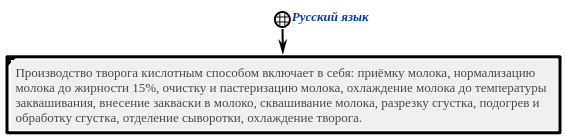
\includegraphics{Contents/part_kb/images/sd_natural_languages/nl_text.png}}
            \begin{scnindent}
            	\scntext{пояснение}{с точки зрения ostis-системы, любой естественно-языкой текст является \textit{файлом.}}
	            \scnrelfrom{лексическая структура}{\scnfileimage[20em]{Contents/part_kb/images/sd_natural_languages/nl_lexical.png}}
			    \begin{scnindent}
		            \scntext{пояснение}{Данная конструкция описывает декомпозицию исходного текста на фрагменты с указанием их принадлежности определённой \textit{номинативной единице} или \textit{знаку алфавита синтаксиса}.}
		            \scnrelfrom{синтаксическая структура}{\scnfileimage[20em]{Contents/part_kb/images/sd_natural_languages/nl_synactical.png}}
		            \bigskip
		            \bigskip
		            \scntext{пояснение}{Здесь приведена только частью синтаксической структуры. Оставшаяся часть записывается аналогично.}
		         \end{scnindent}
        	\end{scnindent}
        \end{scneqtoset}
    \end{scnsubstruct}
    \scnendcurrentsectioncomment
\end{SCn}


\scparagraph[
    \protect\scneditors{Никифоров С.А.;Бобёр  Е.С.}
    \protect\scnmonographychapter{Глава 2.6. Языковые средства формального описания синтаксиса и денотационной семантики различных языков в интеллектуальных компьютерных системах нового поколения}
    ]{Предметная область и онтология синтаксиса естественных языков}
\label{sd_syntax_natural_lang}

\scparagraph[
    \protect\scneditors{Никифоров С.А.;Бобёр  Е.С.}
    \protect\scnmonographychapter{Глава 2.6. Языковые средства формального описания синтаксиса и денотационной семантики различных языков в интеллектуальных компьютерных системах нового поколения}
    ]{Предметная область и онтология денотационной семантики естественных языков}
\label{sd_sem_natural_lang}

\scsubsection[
    \protect\scneditors{Никифоров С.А.;Шункевич Д.В.}
    \protect\scnmonographychapter{Глава 3.1. Формализация понятий действия, задачи, метода, средства, навыка и технологии}
    ]{Глобальная предметная область и онтология, описывающая воздействия, действия, методы, средства и технологии}
\label{sd_actions}
\begin{SCn}
    \scnsectionheader{\currentname}
    \begin{scnsubstruct}
        \begin{SCn}
    \scniselement{раздел}
    \scniselement{предметная область и онтология}
    \begin{scnreltovector}{конкатенация сегментов}
        \scnitem{Уточнение понятия воздействия и понятия действия. Типология воздействий и действий}
        \scnitem{Уточнение понятия задачи. Типология задач}
        \scnitem{Уточнение семейства параметров и отношений, заданных на множестве воздействий, действий и задач}
        \scnitem{Предметная область и онтология субъектно-объектных спецификаций воздействий}
        \scnitem{Уточнение понятий плана сложного действия, класса задач, метода}
        \scnitem{Уточнение понятия навыка, понятия класса методов и понятия модели решения задач}
        \scnitem{Уточнение понятия деятельности, понятия вида деятельности и понятия технологии}
    \end{scnreltovector}
    \bigskip
    \begin{scnhaselementrolelist}{исследуемый класс первичных объектов исследования}
        \scnitem{воздействие}
        \begin{scnindent}
            \scnidtf{\textit{процесс} воздействия одних \textit{сущностей} на другие}
            \scnsubset{процесс}
        \end{scnindent}
        \scnitem{действие}
        \begin{scnindent}
            \scnidtf{\textit{процесс}, \scnqq{осознанно} и целенаправленно выполняемый (управляемый) некоторой \textit{кибернетической системой}}
            \scnsubset{воздействие}
            \scnsubset{процесс}
        \end{scnindent}
        \bigskip
        \scnitem{неосознанное воздействие}
        \bigskip
        \scnitem{действие, выполняемое в памяти субъекта действия}
        \scnitem{действие, выполняемое во внешней среде субъекта действия}
        \scnitem{рецепторное действие}
        \begin{scnindent}
            \scnidtf{действие, выполняемое рецептором субъекта действия}
        \end{scnindent}
        \scnitem{эффекторное действие}
        \begin{scnindent}
            \scnidtf{действие, выполняемое эффектором субъекта действия}
        \end{scnindent}
        \bigskip
        \scnitem{элементарное действие}
        \begin{scnindent}
            \scnidtf{действие, выполнение которого не требует его декомпозиции на взаимосвязанные поддействия}
        \end{scnindent}
        \scnitem{сложное действие}
        \scnitem{легко выполнимое сложное действие}
        \begin{scnindent}
            \scnidtf{сложное действие, которое известно, как выполнять}
        \end{scnindent}
        \scnitem{интеллектуальное действие}
        \begin{scnindent}
            \scnidtf{сложное действие, для которого априори не известно, как его выполнять}
        \end{scnindent}
        \scnitem{индивидуальное действие}
        \begin{scnindent}
            \scnidtf{действие, выполняемое индивидуальной кибернетической системой}
        \end{scnindent}
        \scnitem{коллективное действие}
        \begin{scnindent}
            \scnidtf{действие, выполняемое коллективом кибернетических систем (многоагентной системой)}
        \end{scnindent}
        \bigskip
        \scnitem{планируемое действие}
        \scnitem{инициированное действие}
        \scnitem{выполняемое действие}
        \begin{scnindent}
            \scnidtf{активное действие}
        \end{scnindent}
        \scnitem{прерванное действие}
        \begin{scnindent}
            \scnidtf{выполняемое действие, находящееся в состоянии прерывания}
        \end{scnindent}
        \scnitem{выполненное действие}
        \scnitem{отмененное действие}
        \scnitem{действие с очень высоким приоритетом}
        \scnitem{действие с высоким приоритетом}
        \scnitem{действие со средним приоритетом}
        \scnitem{действие с низким приоритетом}
        \scnitem{действие с очень низким приоритетом}
    \end{scnhaselementrolelist}
    \bigskip
    \begin{scnhaselementrolelist}{исследуемый класс классов первичных объектов исследования}
        \scnitem{осмысленность воздействия\scnsupergroupsign}
        \scnitem{длительность воздействия\scnsupergroupsign}
        \scnitem{место выполнения действия\scnsupergroupsign}
        \scnitem{функциональная сложность действия\scnsupergroupsign}
        \scnitem{многоагентность действия\scnsupergroupsign}
        \begin{scnindent}
            \scnidtf{коллективность субъекта действия}
        \end{scnindent}
        \scnitem{текущее состояние действия\scnsupergroupsign}
        \scnitem{приоритет действия\scnsupergroupsign}
        \begin{scnindent}
            \scnidtf{важность действия\scnsupergroupsign}
        \end{scnindent}
        \scnitem{срочность действия\scnsupergroupsign}
        \bigskip
        \scnitem{класс действий}
        \scnitem{класс функционально эквивалентных действий\scnsupergroupsign}
        \scnitem{класс логически эквивалентных действий\scnsupergroupsign}
        \scnitem{класс семантических эквивалентных задач\scnsupergroupsign}
        \scnitem{класс логически эквивалентных задач\scnsupergroupsign}
        \scnitem{класс задач, для которого существует общий метод их решения\scnsupergroupsign}
        \scnitem{класс аналогичных семантически элементарных процессов воздействия\scnsupergroupsign}
        \begin{scnindent}
            \scnidtf{класс однотипных семантически элементарных воздействий\scnsupergroupsign}
        \end{scnindent}
    \end{scnhaselementrolelist}
    \bigskip
    \begin{scnhaselementrolelist}{исследуемый класс классов}
        \scnitem{отношение, заданное на множестве* (действие)}
        \begin{scnindent}
            \scnidtf{отношение, заданное на множестве действий}
        \end{scnindent}
        \scnitem{отношение, заданное на множестве* (задача)}
        \scnitem{параметр, заданный на множестве* (действие)}
        \scnitem{параметр, заданный на множестве* (задача)}
    \end{scnhaselementrolelist}
    \scnsourcecomment{Здесь указаны классы классов, которые не являются классами классов \uline{первичных} объектов исследования}
    \bigskip
    \begin{scnhaselementrolelist}{исследуемое отношение, заданное на множестве первичных объектов исследования}
        \scnitem{воздействующая сущность\scnrolesign}
        \scnitem{воздействуемая сущность\scnrolesign}
        \scnitem{посредник\scnrolesign}
        \scnitem{медиатор\scnrolesign}
        \scnitem{субъект\scnrolesign}
    	\begin{scnindent}
            \scnidtf{быть субъектом заданного действия}
        \end{scnindent}
        \scnitem{спецификация воздействия*}
    	\begin{scnindent}
            \scnsuperset{спецификация действия*}
        \end{scnindent}
        \scnitem{спецификация действия*}
    	\begin{scnindent}
            \scnsuperset{задача*}
            \begin{scnindent}
	            \begin{scnsubdividing}
		            \scnitem{декларативная формулировка задачи*}
		            \scnitem{процедурная формулировка задачи*}
	            \end{scnsubdividing}
	        \end{scnindent}
            \scnsuperset{план сложного действия*}
            \scnsuperset{декларативная спецификация выполнения сложного действия*}
            \scnsuperset{протокол*}
            \scnsuperset{результативная часть протокола*}
        \end{scnindent}
        \scnitem{декларативная формулировка задачи*}
        \scnitem{процедурная формулировка задачи*}
        \scnitem{план сложного действия*}
        \scnitem{декларативная спецификация выполнения сложного действия*}
        \scnitem{протокол*}
        \scnitem{результативная часть протокола*}
    \end{scnhaselementrolelist}
    \bigskip
    \begin{scnhaselementrolelist}{исследуемое отношение}
        \scnitem{спецификация класса действий*}
        \scnitem{спецификация метода*}
        \scnitem{спецификация класса методов*}
        \scnitem{спецификация деятельности*}
        \scnitem{спецификация вида деятельности*}
    \end{scnhaselementrolelist}
    \begin{scnindent}
    	\scnsourcecomment{Здесь указаны исследуемые отношения, которые заданы не на множестве первичных объектов исследования}	
    \end{scnindent}
    \bigskip
    \begin{scnhaselementrolelist}{исследуемый класс структур, специфицирующих первичные объекты исследования}
        \scnitem{задача}
    	\begin{scnindent}
            \scnidtf{формулировка задачи}
            \scnidtf{спецификация действия}
            \scnidtf{структура (sc-конструкция), содержащая в идеале достаточную информацию для выполнения соответствующего (специфицируемого) действия}
        \end{scnindent}
        \scnitem{декларативная формулировка задачи}
        \begin{scnindent}
            \scnidtf{семантическая спецификация действия}
        \end{scnindent}
        \scnitem{процедурная формулировка задачи}
        \begin{scnindent}
            \scnidtf{функциональная спецификация действия}
        \end{scnindent}
        \scnitem{план сложного действия}
        \begin{scnindent}
            \scnidtf{план выполнения сложного действия}
        \end{scnindent}
        \scnitem{процедурный план сложного действия}
        \scnitem{непроцедурный план сложного действия}
        \begin{scnindent}
            \scnidtf{декларативный план сложного действия}
            \scnidtf{иерархическая система подзадач заданной сложной задачи}
        \end{scnindent}
    \end{scnhaselementrolelist}
    \bigskip
    \begin{scnhaselementrolelist}{исследуемый класс структур}
        \scnitem{метод}
        \begin{scnindent}
            \scnidtf{спецификация класса сложных действий}
        \end{scnindent}
        \scnitem{денотационная семантика метода}
        \scnitem{операционная семантика метода}
        \scnitem{навык}
        \scnitem{модель решения задач}
        \scnitem{технология}
    \end{scnhaselementrolelist}
    \begin{scnindent}
    	\scnsourcecomment{Здесь указаны классы структур, не являющихся спецификациями первичных объектов исследования}
    \end{scnindent}
    \bigskip
    \begin{scnhaselementrolelist}{вводимое, но не исследуемое понятие}
        \scnitem{действие, выполняемое в памяти ostis-системы}
        \scnitem{действие, выполняемое ostis-системой в своей внешней среде}
        \scnitem{рецептурное действие ostis-системы}
        \scnitem{эффекторное действие ostis-системы}
        \scnitem{sc-агент}
    	\begin{scnindent}
            \scnidtf{внутренний субъект ostis-системы}
            \scnidtf{субъект, реализующий действия, выполняемые в памяти ostis-системы}
        \end{scnindent}
    \end{scnhaselementrolelist}
    \begin{scnindent}
    	\scnsourcecomment{Здесь указаны понятия, исследуемые в предметной области (и соответствующей онтологии), которая является \uline{частной} по отношению к заданной и которая наследует все свойства заданной предметной области и онтологии}
    \end{scnindent}
    \bigskip
    \begin{scnhaselementrolelist}{используемое понятие, исследуемое в другой предметной области и онтологии}
        \scnitem{кибернетическая система}
        \begin{scnindent}
            \scnidtf{сущность, обладающая способностью быть субъектом различного вида действий}
        \end{scnindent}
        \scnitem{компьютерная система}
        \begin{scnindent}
            \scnidtf{искусственная кибернетическая система}
            \scnsubset{кибернетическая система}
        \end{scnindent}
        \scnitem{интеллектуальная компьютерная система}
        \begin{scnindent}
            \scnsubset{компьютерная система}
            \scnsuperset{ostis-система}
        \end{scnindent}
        \scnitem{человек}
        \begin{scnindent}
            \scnsubset{кибернетическая система}
        \end{scnindent}
        \scnitem{ostis-система}
        \scnitem{спецификация*}
        \begin{scnindent}
            \scnidtf{быть спецификацией (описанием, семантической окрестностью заданной сущности*)}
            \scnidtf{семантическая окрестность*}
        \end{scnindent}
    \end{scnhaselementrolelist}
   
    \scnheader{следует отличать*}
    \begin{scnhaselementset}
        \scnitem{\scnnonamednode}
        \begin{scnindent}
            \begin{scneqtovector}
                \scnitem{действие}
                \scnitem{класс действий}
            \end{scneqtovector}
        \end{scnindent}
        \scnitem{\scnnonamednode}
        \begin{scnindent}
            \begin{scneqtovector}
                \scnitem{метод}
                \scnitem{класс методов}
            \end{scneqtovector}
        \end{scnindent}
        \scnitem{\scnnonamednode}
        \begin{scnindent}
            \begin{scneqtovector}
                \scnitem{деятельность}
                \scnitem{вид деятельности}
            \end{scneqtovector}
        \end{scnindent}
    \end{scnhaselementset}
    \begin{scnindent}
	    \scnsubset{семейство подклассов*}
	    \scntext{примечание}{Все сущности, принадлежащие рассмотренным \textit{понятиям}, требуют достаточно детальной \textit{спецификации}. При этом не следует путать сами сущности и их \textit{спецификации}. Так, например, не следует путать \textit{действие} и \textit{задачу}, которая специфицирует (уточняет) это \textit{действие}. Особое место среди указанных понятий занимает понятие \textit{метода}, т.к. каждый конкретный \textit{метод}, с одной стороны, является \textit{спецификацией} соответствующего \textit{класса действий}, а, с другой стороны, сам нуждается в \textit{спецификации}, которая уточняет либо \textit{декларативную семантику} этого \textit{метода} (т.е. обобщенную декларативную формулировку класса задач, решаемых с помощью этого \textit{метода}), либо \textit{операционную семантику} этого \textit{метода}, (т.е. множество \textit{методов}, обеспечивающих \textit{интерпретацию} данного специфицируемого \textit{метода}) и тем самым преобразует специфицируемый \textit{метод} в \textit{навык}.}
    \end{scnindent}
    	
    \scnheader{следует отличать*}
    \begin{scnhaselementvector}
        \scnitem{первый домен*(спецификация*)}
        \begin{scnindent}
            \scnidtf{специфицируемая сущность}
            \scnidtf{сущность, использование которой требует вполне определенной ее спецификации}
            \scnsuperset{действие}
            \scnsuperset{класс действий}
            \scnsuperset{метод}
            \scnsuperset{класс методов}
            \scnsuperset{деятельность}
            \scnsuperset{вид деятельности}
        \end{scnindent}
        \scnitem{второй домен*(спецификация*)}
    	\begin{scnindent}
            \scnidtf{спецификация}
            \scnsuperset{задача}
            \begin{scnindent}
	            \scnsuperset{декларативная формулировка задачи}
	            \begin{scnindent}
	            	\scnidtf{семантическая формулировка задачи}
	            \end{scnindent}
	            \scnsuperset{процедурная формулировка задачи}
	            \begin{scnindent}
	            	\scnidtf{функциональная формулировка задачи}
	            \end{scnindent}
	        \end{scnindent}
            \scnsuperset{план действия}
            \begin{scnindent}
	            \scnidtf{план}
	            \scnidtf{план выполнения действия}
	    	\end{scnindent}
            \scnsuperset{декларативная спецификация выполнения действий}
            \begin{scnindent}
            	\scnidtf{иерархическая система подзадач}
            \end{scnindent}
            \scnsuperset{протокол}
            \scnsuperset{результативная часть протокола}
            \scnsuperset{обобщенная декларативная формулировка класса задач}
            \scnsuperset{метод}
            \scnsuperset{декларативная семантика метода}
            \scnsuperset{операционная семантика метода}
            \scnsuperset{модель решения задач}
        \end{scnindent}
    \end{scnhaselementvector}
	\begin{scnindent}
    	\scntext{примечание}{При этом следует отличать:
	        \begin{scnitemize}
	            \item спецификацию конкретного \textit{действия} (\textit{задачу}, \textit{план}, \textit{декларативную спецификацию выполнения действия}, \textit{протокол}, \textit{результативную часть протокола});
	            \item спецификацию конкретной \textit{деятельности} (\textit{контекст}*, \textit{множество используемых методов}*);
	            \item спецификацию \textit{класса действий} (\textit{обобщенную декларативную формулировку класса задач}, \textit{метод});
	            \item спецификацию \textit{вида деятельности} (\textit{технологию});
	            \item спецификацию \textit{метода} (\textit{декларативную семантику метода}, \textit{операционную семантику метода});
	            \item спецификацию \textit{класса методов} (\textit{модель решения задач}).
	        \end{scnitemize}}
    \end{scnindent}
    
    \scnheader{следует отличать*}
    \begin{scnhaselementset}
        \scnitem{\scnnonamednode}
        \begin{scnindent}
            \begin{scneqtovector}
		      \scnitem{действие}
		      \scnitem{класс действий, метод}
            \end{scneqtovector}
        \end{scnindent}
        \scnitem{\scnnonamednode}
        \begin{scnindent}
            \begin{scneqtovector}
             \scnitem{деятельность}
             \scnitem{вид деятельности, технология}
            \end{scneqtovector}
        \end{scnindent}
    \end{scnhaselementset}
    
    \bigskip
    
    %в стандарте нет этого
    \begin{scnrelfromlist}{библиографический источник}
        \scnitem{\cite{Martynov1984}}
        \begin{scnindent}
            \scnciteannotation{Martynov1984}
    	\end{scnindent}
        \scnitem{\cite{Ikeda1998}}
    	\begin{scnindent}
            \scnciteannotation{Ikeda1998}
            \scnrelfrom{ключевой знак}{онтология классов задач}
        	\begin{scnindent}
	            \scnidtf{задачная онтология}
	            \scnidtf{онтология классов задач, решаемых в данной предметной области}
        	\end{scnindent}
        \end{scnindent}
        \scnitem{\cite{Studer1996}}
        \begin{scnindent}
            \scnciteannotation{Studer1996}
     	\end{scnindent}
        \scnitem{\cite{Benjamins1999}}
        \begin{scnindent}
            \scnciteannotation{Benjamins1999}
        \end{scnindent}
        \scnitem{\cite{Chandrasekaran1999}}
        \begin{scnindent}
            \scnciteannotation{Chandrasekaran1999}
        \end{scnindent} 
        \scnitem{\cite{Chandrasekaran1998}}
        \begin{scnindent}
            \scnciteannotation{Chandrasekaran1998}
        \end{scnindent}
        \scnitem{\cite{Fensel1998Reuse}}
        \begin{scnindent}
            \scnciteannotation{Fensel1998Reuse}
        \end{scnindent}
        \scnitem{\cite{Kemke2001}}
        \begin{scnindent}
            \scnciteannotation{Kemke2001}
    	\end{scnindent}
        \scnitem{\cite{Tu1995}}
        \begin{scnindent}
            \scnciteannotation{Tu1995}
        \end{scnindent}
        \scnitem{\cite{Trypuz2007}}
        \begin{scnindent}
            \scnciteannotation{Trypuz2007}
        \end{scnindent}
        \scnitem{\cite{Fang2019}}
        \begin{scnindent}
            \scnciteannotation{Fang2019}
        \end{scnindent}
        \scnitem{\cite{Fensel1997}}
        \scnitem{\cite{McBride2021}}
        \begin{scnindent}
            \scnciteannotation{McBride2021}
        \end{scnindent}
        \scnitem{\cite{Crowther2020}}
        \begin{scnindent}
            \scnciteannotation{Crowther2020}
        \end{scnindent}
        \scnitem{\cite{McCann1998}}
        \begin{scnindent}
            \scnciteannotation{McCann1998}
        \end{scnindent}
        \scnitem{\cite{Yan2014}}
        \begin{scnindent}
            \scnciteannotation{Yan2014}
        \end{scnindent}
        \scnitem{\cite{Ansari2018}}
        \scnitem{\cite{Crubezy2004}}
        \begin{scnindent}
            \scnciteannotation{Crubezy2004}
        \end{scnindent}
        \scnitem{\cite{Coelho1996}}
    \end{scnrelfromlist}
\end{SCn}

        \begin{SCn}
    \scnsegmentheader{Уточнение понятия воздействия и понятия действия. Типология воздействий и действий}
    \begin{scnsubstruct}
        \scniselement{сегмент базы знаний}
        
        \scnheader{воздействие}
        \scnidtf{\textit{процесс} воздействия одной сущности (или некоторого множества \textit{сущностей}) на другую \textit{сущность} (или на некоторое множество других \textit{сущностей})}
        \scnidtf{\textit{процесс}, в котором могут быть явно выделены хотя бы одна воздействующая сущность (\textit{субъект воздействия\scnrolesign}) и хотя бы одна \textit{сущность}, на которую осуществляется воздействие (\textit{субъект воздействия\scnrolesign})}
        
        \scnheader{воздействие}
        \scnsubset{процесс}
        \begin{scnindent}
        	\scnidtf{динамическая структура}
        \end{scnindent}
        \scntext{примечание}{Поскольку \textit{воздействия} являются частным видом \textit{процессов}, воздействиями наследуются все свойства \textit{процессов}. Смотрите Раздел \textit{Предметная область и онтология структур}). В частности, используются все \textit{параметры}, заданные на множестве \textit{процессов}, например, \textit{длительность*}, \textit{момент начала процесса*}, \textit{момент завершения процесса\scnsupergroupsign}}
        
        \scnheader{процесс}
        \scnrelfrom{покрытие}{длительность\scnsupergroupsign}
    	\begin{scnindent}
            \begin{scneqtoset}
                \scnitem{краткосрочный процесс}
                \scnitem{среднесрочный процесс}
                \scnitem{долгосрочный процесс}
                \scnitem{перманентный процесс}
            \end{scneqtoset}
            \scntext{примечание}{Длительность различных процессов можно уточнять до любой необходимой точности, используя различные единицы измерения длительности (с точностью до секунд, минут, часов, дней, месяцев, лет, столетий и т.д.). Кроме того, можно ссылаться на процессы, длительность (время жизни) которых соизмерима с рассматриваемым процессом.}
        \end{scnindent}
        
        \scnheader{действие}
        \scnsubset{воздействие}
        \begin{scnindent}
        	\scnsubset{процесс}
        \end{scnindent}
        \scnidtf{\textit{воздействие}, в котором \textit{воздействующая сущность\scnrolesign} осуществляет \textit{воздействие} осознанно, целенаправленно}
        \scnidtf{целенаправленный процесс, выполняемый одним или несколькими субъектами (кибернетическими системами) с возможным применением некоторых инструментов}
        \scnidtf{акция}
        \scnidtf{акт}
        \scnidtf{операция}
        \scnidtf{\uline{процесс} воздействия некоторой (возможно, коллективной) сущности (субъекта воздействия) на некоторую одну или несколько сущностей (объектов воздействия - исходных объектов (аргументов) или целевых (создаваемых или модифицируемых) объектов)}
        \scnidtf{осознанное воздействие}
        \scnidtf{активное воздействие}
        \scnidtf{целеноправленный (осознанный) процесс, выполняемый (управляемый, реализуемый) неким субъектом}
        \scnidtf{акция реализации некоторого замысла}
        \scnidtf{преднамеренная акция}
        \scnidtf{работа}
        \scnidtf{процесс выполнения некоторой задачи}
        \scnidtf{дело}
        \scnidtf{целостный фрагмент некоторой деятельности}
        \scnidtf{целенаправленный процесс, управляемый некоторым субъектом (возможно, коллективным)}
        \scnidtf{целенаправленный процесс, выполняемый некоторым субъектом (исполнителем) над некоторыми объектами}
        \scntext{примечание}{Каждое \textit{действие}, выполняемое тем или иным \textit{субъектом}, трактуется как процесс решения некоторой задачи, т.е. процесс достижения заданной цели в заданных условиях, и, следовательно, выполняется целеноправленно. При \textit{этом} явное указание \textit{действия} и его связи с конкретной задачей может не всегда присутствовать в памяти. Некоторые \textit{задачи} могут решаться определенными агентами перманентно, например, оптимизация \textit{базы знаний}, поиск некорректностей и т.д. и для подобных задач не всегда есть необходимость явно вводить \textit{структуру}, являющуюся формулировкой \textit{задачи}.\\
        	Каждое \textit{действие} может обозначать сколь угодно малое преобразование, осуществляемое во внешней среде либо в памяти некоторой \textit{кибернетической системы}, однако в памяти явно вводятся знаки только тех \textit{действий}, для которых есть небходимость явно хранить в памяти их спецификацию в течение некоторого времени.При выполнении \textit{действия} можно выделить этапы:
            \begin{scnitemize}
                \item построение \textit{плана действия}, декомпозиция (детализация) действия в виде системы его \textit{поддействий};
                \item выполнение построенного плана \textit{действия}
            \end{scnitemize}}
        \scntext{правило идентификации экземпляров}{Экземпляры класса \textit{действий} в рамках \textit{Русского языка} именуются по следующим правилам:
            \begin{scnitemize}
                \item в начале идентификатора пишется слово ``\textit{Действие}'' и ставится точка;
                \item далее с прописной буквы идет либо содержащее глагол совершенного вида в инфинитиве описание сути того, что требуется получить в результате выполнения действия, либо вопросительное предложение, являющееся спецификацией запрашиваемой (ответной) информации.
            \end{scnitemize}
            Например:\\
            \textit{Действие. Сформировать полную семантическую окрестность понятия треугольник}\\
            \textit{Действие. Верифицировать Раздел. Предметная область sc-элементов}}
            
        \scnheader{следует отличать*}
        \begin{scnhaselementset}
            \scnitem{действие}
        	\begin{scnindent}
                \scntext{примечание}{Каждому \textit{действию} становится в соответствие \textit{кибернетическая система}, являющаяся \textit{субъектом} этого \textit{действия}. Указанный \textit{субъект} может быть либо \textit{индивидуальной}, либо \textit{коллективной кибернетической системой}.}
            \end{scnindent}
            \scnitem{воздействие}
        	\begin{scnindent}
                \scnsuperset{действие}
                \scnsubset{процесс}
                \scntext{примечание}{Сущностью, осущетвляющей воздействие на какой-либо объект, может быть не только \textit{кибернетическая система}, но также, например, и пассивный инструмент, управляемый некоторой \textit{кибернетической системой}.}
            \end{scnindent}
            \scnitem{деятельность}
        \end{scnhaselementset}
        
        \scnheader{параметр, заданный на множестве* (воздействие)}
        \scnidtf{признак классификации воздействий}
        \scnhaselement{осознанность воздействия\scnsupergroupsign}
        \begin{scnindent}
	        \scnidtf{Наличие субъекта (индивида), который запланировал и реализовал воздействие, т.е. обеспечил управление выполнением этого воздействия}
	        \begin{scneqtoset}
	            \scnitem{неосознанное действие}
	            \scnitem{действие}
	            \begin{scnindent}
	            	\scnidtf{осознанное действие}
	            \end{scnindent}
	        \end{scneqtoset}
        \end{scnindent}
        
        \scnheader{параметр, заданный на множестве* (действие)}
        \scnidtf{признак классификации действий}
        \scnhaselement{место выполнения действия\scnsupergroupsign}
        \scnhaselement{функциональная сложность действия\scnsupergroupsign}
        \scnhaselement{многоагентность выполнения действия\scnsupergroupsign}
        \scnhaselement{текущее состояние действия\scnsupergroupsign}
        \scnhaselement{приоритет действия\scnsupergroupsign}
        
        \scnheader{действие}
        \scnrelfrom{разбиение}{место выполнения действия\scnsupergroupsign}
        \begin{scnindent}
	        \begin{scneqtoset}
	            \scnitem{действие, выполняемое в памяти субъекта действия}
	            \scnitem{действие, выполняемое во внешней среде субъекта действия}
	            \scnitem{рецепторное действие}
	            \scnitem{эффекторное действие}
	        \end{scneqtoset}
        \end{scnindent}
        \scnrelfrom{разбиение}{функциональная сложность действия\scnsupergroupsign}
        \begin{scnindent}
	        \begin{scneqtoset}
	            \scnitem{элементарное действие}
	            \begin{scnindent}
	            	\scnidtf{действие, выполняемое индивидуальной кибернетической системой}
	                \scntext{пояснение}{Элементарное действие выполняется одним индивидуальным субъектом и является либо элементарным действием, выполняемым в памяти этого субъекта (элементарным действием его процессора), либо элементарным действием одного из его эффекторов.}
	            \end{scnindent}
	            \scnitem{сложное действие}
	        	\begin{scnindent}
	                \scnidtf{неэлементарное действие}
	                \scnidtf{действие выполнение которого требует декомпозиции этого действия на множество его \uline{поддействий}, т.е. частных действий более низкого уровня}
	                \scntext{примечание}{Декомпозиция сложного действия на поддействия может иметь весьма сложный иерархический вид с большим числом уровней иерархии, т.е. поддействиями \textit{сложного действия} могут также \textit{сложные действия}. Уровень сложности действия можно определять (1) общим числом его поддействий и (2) числом уровней иерархии этих поддействий.}
	                \scntext{примечание}{Другим примером может служить запись одной и той же процедурной программы на языке программирования более высокого уровня и на языке программирования более низкого уровня. В данном случае элементарность действий строго определяется на уровне языка.}
	                \scntext{примечание}{Темпоральные соотношения между \textit{поддействиями} сложного \textit{действия} могут быть самые различные, но в пройстейшем случае \textit{сложное действие} представляет собой строгую последовательность \textit{действий} более низкого уровня иерархии.}
	                \scnidtf{система более простых действий (\textit{поддействий}), которые могут выполняться как последовательно, так и параллельно}
	                \scntext{примечание}{В состав \textit{сложного действия} могут входить не только \textit{собственно поддействия} этого \textit{сложного действия}, но также и специальные \textit{поддействия}, осуществляющие \uline{управление} процессом выполнения \textit{сложного действия}, и, в частности, \textit{поддействия}, осуществляющие инициирование поддействий, передачу управления \textit{поддействиям}.}
	                \scnidtf{неатомарное действие}
	                \scnidtf{неэлементарное \textit{действие}}
	                \scnidtf{\textit{действие}, выполнение которого сводится в общем случае к последовательно-параллельному выполнению некоторого множества \textit{поддействий}}
	                \scnidtf{\textit{действие}, декомпозируемое на множество более простых \textit{действий} (\textit{поддействий}), обеспечивающих выполнение исходного (заданного) \textit{действия}}
	                \begin{scnrelfromset}{покрытие}
	                    \scnitem{легко выполнимое сложное действие}
	                	\begin{scnindent}
	                        \scnidtf{сложное действие, для выполнения которого известен соответствующий \textit{метод} и соответствующие этому методу исходные данные, а также (для действий, выполняемых во внешней среде) имеются в наличии все необходимые исходные объекты (расходные материалы и комплектация), а также средства (инструменты)}
	                    \end{scnindent}
	                    \scnitem{интеллектуальное действие}
	                	\begin{scnindent}
	                        \scnidtf{трудно выполнимое сложное действие}
	                        \scnidtf{сложное действие, для выполнения которого в текущий момент либо неизвестен соответствующий \textit{метод}, либо возможные \textit{методы} известны, но отсутствуют условия их применения.}
	                        \scnsuperset{действие, у которого цель известна, на зачада не совсем точна}
	                        \begin{scnindent}
		                        \scnsuperset{действие, направленное на выявление противоречий в базе знаний}
		                        \begin{scnindent}
		                        	\scntext{примечание}{Это действие декомпозируется на несколько самостоятельных поддействий, каждое из которых выявляет (локализует) противоречия (ошибки) конкретного формализуемого вида, для которого в базе знаний существует точное определение}
		                        \end{scnindent}
		                    \end{scnindent}
	                        \scnsuperset{действие, для которого априори не известен метод, обеспечивающий его выполнение}
	                        \begin{scnindent}
	                        	\scntext{примечание}{Соответствующий метод либо не найден, либо его вообще нет в памяти.}
	                        \end{scnindent}
	                    \end{scnindent}
	                \end{scnrelfromset}
	            \end{scnindent}
	        \end{scneqtoset}
	    \end{scnindent}
        \scnrelfrom{разбиение}{многоагентность выполнения действия\scnsupergroupsign}
        \begin{scnindent}
	        \begin{scneqtoset}
	            \scnitem{индивидуальное действие}
	        	\begin{scnindent}
	            	\scnidtf{действие, выполняемое одним субъектом (агентом)}
	                \scnidtf{действие, выполняемое индивидуальной кибернетической системой}
	                \scnsuperset{индивидуальное действие, выполняемое человеком}
	                \scnsuperset{индивидуальное действие, выполняемое компьютерной системой}
	            \end{scnindent}
	            \scnitem{\textit{коллективное} действие}
	        	\begin{scnindent}
	            	\scnidtf{действие, выполняемое коллективом субъектов (многоагентной системой)}
	                \scnidtf{действие, выполняемое коллективом кибернетических систем (коллективом субъектов)}
	                \scnsuperset{действие, выполняемое коллективом людей}
	                \scnsuperset{действие, выполняемое коллективом индивидуальных компьютерных систем}
	                \scnsuperset{действие, выполняемое коллективом людей и индивидуальных компьютерных систем}
	                \begin{scnindent}
		                \scnsuperset{действие, выполняемое Экосистемой OSTIS}
		                \scnsuperset{действие, выполняемое одним человеком во взаимодействии с одной индивидуальной компьютерной системой}
		            \end{scnindent}
	            \end{scnindent}
        	\end{scneqtoset}
        \end{scnindent}
        \scnrelfrom{разбиение}{текущее состояние действия\scnsupergroupsign}
        \begin{scnindent}
	        \begin{scneqtoset}
		            %TODO: check by human--->
		            \scnitem{планируемое действие}
		            \begin{scnindent}
		                \scnidtf{запланированное, но не инициированное действие}
		                \scnidtf{будущее действие}
		                \scnidtf{действие, которое планируется выполнить в будущем}
		                \scntext{пояснение}{Во множество \textit{запланированных, но не инициированных действий} входят \textit{действия}, начать выполнение которых запланировано на какой-либо момент в будущем.}
		            \end{scnindent}
		            \scnitem{инициированное действие}
		            \begin{scnindent}
		                \scnidtf{инициированное, но не выполняемое действие}
		                \scnidtf{действие, подлежащее выполнению}
		                \scnidtf{действие, включенное в план}
		                \scnidtf{действие, ожидающее начала своего выполнения}
		                \scntext{пояснение}{Во множество \textit{инициированных действий} входят \textit{действия}, выполнение которых инициировано в результате какого-либо события.В общем случае, \textit{действия} могут быть инициированы по следующим причинам:
		                    \begin{scnitemize}
		                        \item явно путем проведения соответствующей \textit{sc-дуги принадлежности} каким-либо \textit{субъектом (заказчиком*)}. В случае действия в \textit{sc-памяти}, оно может быть инициировано как внутренним \textit{sc-агентом} системы, так и пользователем при помощи соответствующего пользовательского интерфейса. При этом, спецификация действия может быть сформирована одним \textit{sc-агентом}, а собственно добавление во множество \textit{инициированных действий} может быть осуществлено позже другим \textit{sc-агентом}
		                        \item в результате того, что одно или несколько \textit{действий}, предшествовавших данному в рамках некоторой декомпозиции, стали \textit{прошлыми сущностями} (процедурный подход)
		                        \item в результате того, что в \textit{памяти} системы появилась конструкция, соответствующая некоторому условию инициирования \textit{sc-агента}, который должен выполнить данное \textit{действие} (декларативный подход).
		                    \end{scnitemize}
		                    Следует отметить, что декларативный и процедурный подходы можно рассматривать как две крайности, использование только одной из которых не является удобным и целесообразным. При этом, например, принципы инициирования по процедурному подходу могут быть полностью сведены к набору декларативных условий инициирования, но как было сказано, это не всегда удобно и наиболее рациональным будет комбинировать оба подхода в зависимости от ситуации.По сути, попадание некоторого \textit{действия} во множество \textit{инициированных действий} говорит о том, что, по мнению некоторого \textit{субъекта} (заказчика, инициатора), оно готово к выполнению и должно быть выполнено, то есть спецификация данного \textit{действия} по мнению данного \textit{субъекта} сформирована в степени, достаточной для решения поставленной \textit{задачи} и существует некоторый другой \textit{субъект} (исполнитель), который может приступать к выполнению \textit{действия}. Однако стоит отметить, что с точки зрения \textit{исполнителя} такая спецификация \textit{действия} в общем случае может оказаться недостаточной или некорректной.}
		            \end{scnindent}
		            \scnitem{выполняемое действие}
		            \begin{scnindent}
		                \scnidtf{активное действие}
		                \scnidtf{непосредственно выполняемое действие}
		                \scnidtf{действие, выполняемое в текущий момент}
		                \scnidtf{настоящее действие}
		                \scniselement{неосновное понятие}
		                \scnsubset{настоящая сущность}
		                \scntext{пояснение}{Во множество \textit{выполняемых действий} входят \textit{действия}, к выполнению которых приступил какой-либо из соответствующих \textit{субъектов}.Попадание \textit{действия} в данное множество говорит о следующем:
		                    \begin{scnitemize}
		                        \item рассматриваемое \textit{действие} уже попало во множество \textit{инициированных действий}.
		                        \item существует как минимум один \textit{субъект}, условие инициирования которого соответствует спецификации данного \textit{действия}.
		                    \end{scnitemize}
		                    После того, как собственно процесс выполнения завершился, \textit{действие} должно быть удалено из множества \textit{выполняемых действий} и добавлено во множество \textit{выполненных действий} или какое-либо из его подмножеств.Понятие \textit{выполняемое действие} является неосновным, и вместо того, чтобы относить конкретные действия к данному классу, их относят к классу \textit{настоящих сущностей}.}
		            \end{scnindent}
		            \scnitem{прерванное действие}
		            \begin{scnindent}
		                \scnidtf{действие, ожидающее продолжения своего выполнения}
		                \scnidtf{отложенное действие}
		                \scnidtf{приостановленное действие}
		                \scntext{пояснение}{Во множество \textit{прерванных действий} входят \textit{действия}, которые уже были инициированы, однако их выполнение невозможно по каким-либо причинам, например в случае, когда у исполнителя в данный момент есть более приоритетные задачи.}
		            \end{scnindent}
		            \scnitem{выполненное действие}
		            \begin{scnindent}
		                \scnidtf{завершенное действие}
		                \scnidtf{прошлое действие}
		                \scniselement{неосновное понятие}
		                \scnsubset{прошлая сущность}
		                \scntext{пояснение}{Во множество \textit{выполненных действий} попадают \textit{действия}, выполнение которых с \uline{точки зрения \textit{субъекта}}, осуществлявшего их выполнение. Таким образом, понятие \textit{выполненного действия} является относительным, поскольку с точки зрения разных субъектов одно и то же действие может считаться выполненным или все еще выполняющимся.\\
		                	В зависимости от результатов конкретного процесса выполнения, рассматриваемое \textit{действие} может стать элементом одного из подмножеств множества \textit{выполненных действий}.Понятие \textit{выполненное действие} является неосновным, и вместо того, чтобы относить конкретные \textit{действия} к данному классу, их относят к классу \textit{прошлых сущностей}.}
			                \begin{scnsubdividing}
			                    \scnitem{успешно выполненное действие}
			                    \begin{scnindent}
			                        \scntext{пояснение}{Во множество \textit{успешно выполненных действий} попадают \textit{действия}, выполнение которых успешно завершено с точки зрения \textit{субъекта}, осуществлявшего их выполнение, т.е. достигнута поставленная цель, например, получены решение и ответ какой-либо задачи, успешно преобразована какая-либо конструкция и т.д. Очень важно отметить, что в общем случае выделить критерии успешности или безуспешности выполнения действий того или иного класса \uline{невозможно}, поскольку эти критерии, во-первых, зависят от контекста, во-вторых, могут быть разными с точки зрения разных субъектов. Однозначно критерии успешности выполнения действий могут быть сформулированы для некоторых частных классов действий, например, классов операторов некоторого процедурного языка программирования (например, \textit{scp-операторов}).\\
			                         Таким образом, понятие \textit{успешно выполненное действие} является относительным.\\
			                         Если действие было выполнено успешно, то, в случае действия по генерации каких-либо знаний, к \textit{действию} при помощи связки отношения \textit{результат*} приписывается \textit{sc-конструкция}, описывающая результат выполнения указанного действия. В случае, когда действие направлено на какие-либо изменения базы знаний, \textit{sc-конструкция}, описывающая результат действия, формируется в соответствии с правилами описания истории изменений базы знаний.\\
			                         В случае, когда успешное выполнение \textit{действия} приводит к изменению какой-либо конструкции в \textit{sc-памяти}, которое необходимо занести в историю изменений базы знаний или использовать для демонстрации протокола решения задачи, то генерируется соответствующая связка отношения \textit{результат*}, связывающая задачу и \textit{sc-конструкцию}, описывающую данное изменение.}
			              		\end{scnindent}
			              		%слишком большой отступ
			                    \scnitem{безуспешно выполненное действие}
			                    \begin{scnindent}
			                        \scntext{пояснение}{Во множество \textit{безуспешно выполненных действий} попадают \textit{действия}, выполнение которых не было успешно завершено с точки зрения \textit{субъекта}, осуществлявшего их выполнение, по каким-либо причинам.Можно выделить две основные причины, по которым может сложиться указанная ситуация:
			                            \begin{scnitemize}
			                                \item соответствующая \textit{задача} сформулирована некорректно
			                                \item формулировка соответствующей \textit{задачи} корректна и понятна системе, однако решение данной задачи в текущий момент не может быть получено за удовлетворительное с точки зрения заказчика или исполнителя сроки.
			                            \end{scnitemize}
			                            Для конкретизации факта некорректности формулировки задачи можно выделить ряд более частных классов \textit{безуспешно выполненных действий}, например:
			                            \begin{scnitemize}
			                                \item действие, спецификация которого противоречит другим знаниям системы (например, не выполняется неравенство треугольника)
			                                \item действие, при спецификации которого использованы понятия, неизвестные системе
			                                \item действие, выполнение которого невозможно из-за недостаточности данных (например, найти площадь треугольника по двум сторонам)
			                                \item и другие.
			                            \end{scnitemize}
			                            Для конкретизации факта безуспешности выполнения некоторого действия в системе могут также использоваться дополнительные подмножества данного множества, при необходимости снабженные естественно-языковыми или формальными комментариями.}
			                        \scnsuperset{действие, выполненное с ошибкой}
			                        \begin{scnindent}
			                        	\scntext{пояснение}{Во множество \textit{действий, выполненных с ошибкой}, попадают \textit{действия}, выполнение которых не было успешно завершено с точки зрения \textit{субъекта}, осуществлявшего их выполнение, по причине возникновения какой-либо ошибки, например, некорректности спецификации данного \textit{действия} или нарушения её целостности каким-либо \textit{субъектом} (в случае \textit{действия в sc-памяти}).}
			                        \end{scnindent}
			                  \end{scnindent}
					\end{scnsubdividing}
					\end{scnindent}
		            \scnitem{отмененное действие}
	        \end{scneqtoset}
	    \end{scnindent}
        \scnrelfrom{покрытие}{приоритет действия\scnsupergroupsign}
        \begin{scnindent}
	        \begin{scneqtoset}
	            \scnitem{действие с очень высоким приоритетом}
	            \scnitem{действие с высоким приоритетом}
	            \scnitem{действие со средним приоритетом}
	            \scnitem{действие с низким приоритетом}
	            \scnitem{действие с очень низким приоритетом}
	        \end{scneqtoset}
        \end{scnindent}
        	
        \scnheader{действие, выполняемое в памяти субъекта действия}
        \scnidtf{информационное действие}
        \scnidtf{действие, выполняемое в памяти}
        \scnidtf{действие кибернетической системы, направленное на обработку информации, хранимой в её памяти}
        \scnsuperset{действие, выполняемое кибернетической системой в собственной памяти и направленное на организацию её деятельности во внешней среде}
        \begin{scnindent}
        	\scnidtf{действие, выполняемое кибернетической системой в её памяти и направленное на организацию её деятельности во внешней среде и в конечном счете --- на сенсо-моторную координацию деятельности её эффекторов}
        \end{scnindent}
        \scntext{пояснение}{Результатом выполнения \textit{действия, выполняемого в памяти субъекта действия} является в общем случае некоторое новое состояние памяти информационной системы (не обязательно \textit{sc-памяти}), достигнутое исключительно путем преобразования информации, хранящееся в памяти системы, то есть либо посредством генерации новых знаний на основе уже имеющихся, либо посредством удаления знаний, по каким-либо причинам ставших ненужными. Следует отметить, что если речь идет об изменении состояния \textit{sc-памяти}, то любое преобразование информации можно свести к ряду элементарных действий генерации, удаления или изменения инцидентности \textit{sc-элементов} друг относительно друга.}
        
        \scnheader{действие, выполняемое во внешней среде субъекта действия}
        \scnidtf{действие, выполняемое кибернетической системой в её внешней среде и осуществляемое (на самом низком уровне) эффекторами этой кибернетической системы}
        \scnidtf{поведенческое действие}
        \scntext{пояснение}{В случае \textit{действия, выполняемого во внешней среде субъекта действия} результатом его выполнения будет новое состояние внешней среды. Очень важно отметить, что под внешней средой в данном случае понимаются также и компоненты системы, внешние с точки зрения памяти, то есть не являющиеся хранимыми в ней информационными конструкциями. К таким компонентам можно отнести, например, различные манипуляторы и прочие средства воздействия системы на внешний мир, то есть к поведенческим задачам можно отнести изменение состояния механической конечности робота или непосредственно вывод некоторой информации на экран для восприятия пользователем.}
        
        \scnheader{поддействие*}
        \scnidtf{быть поддействием заданного \textit{сложного действия*}}
        \begin{scnsubdividing}
            \scnitem{собственное поддействие*}
            \scnitem{управляющее поддействие*}
            \begin{scnindent}
                \scntext{пояснение}{\textit{поддействие*}, которое осуществляет инициирование выполнения очередного \textit{поддействия*} (или сразу некоторого множества \textit{поддействий*}) при соблюдении некоторого априори известного условия.В общем случае таким условием является возникновение некоторой ситуации или события. В частности, это может быть:
                    \begin{scnitemize}
                        \item ситуация или событие в обрабатываемой \textit{базе знаний} (это называют условной передачей управления)
                        \item факт успешного завершения некоторого \textit{поддействия} (это безусловная передача управления)
                        \item факт успешного завершения \uline{по крайней мере одного} из заданного множества \textit{поддействий}
                        \item факт успешного завершения \uline{всех} \textit{поддействий} из заданного множества \textit{поддействий}.
                    \end{scnitemize}}
                \scntext{примечание}{На самом деле при выполнении \textit{сложных действий} многообразие условий инициирования (передачи управления) поддействиям может быть значительно шире}
           \end{scnindent}
        \end{scnsubdividing}
        \bigskip
    \end{scnsubstruct}
    \scnendsegmentcomment{Уточнение понятия воздействия и понятия действия. Типология воздействий и действий}
\end{SCn}

        \begin{SCn}
    \scnsegmentheader{Уточнение понятия задачи. Типология задач}
    \begin{scnsubstruct}
        \scniselement{сегмент базы знаний}
        
        \scnheader{задача}
        \scnidtf{описание желаемого состояния или события в рамках внешней среды кибернетической системы либо в рамках её базы знаний}
        \scnidtf{формулировка задачи}
        \scnidtf{задание на выполнение некоторого действия}
        \scnidtf{постановка задачи}
        \scnidtf{описание задачной ситуации}
        \scnidtf{спецификация некоторого действия, обладающая достаточной полнотой для выполнения этого действия}
        \scnidtf{цель плюс дополнительные условия (ограничения) накладываемые на результат или процесс получения этого результата}
        \scnidtf{описание того, что требуется сделать}
        \scntext{пояснение}{\textbf{\textit{Задача}}, т.е. формальное описание условия некоторой задачи есть, по сути, формальная \textit{спецификация} некоторого \textit{действия}, направленного на решение данной \textit{задачи}, достаточная для выполнения данного \textit{действия} каким-либо \textit{субъектом}. В зависимости от конкретного \textit{класса задач}, описываться может как внутреннее состояние самой интеллектуальной системы, так и требуемое состояние \textit{внешней среды}. \textit{sc-элемент}, обозначающий \textit{действие} входит в \textit{задачу} под атрибутом \textit{ключевой знак\scnrolesign}.\\
            Каждая \textbf{\textit{задача}} представляет собой спецификацию \textit{действия}, которое либо уже выполнено, либо выполняется в текущий момент (в настоящее время), либо планируется (должно) быть выполненным, либо может быть выполнено (но не обязательно).\\
            Классификация \textit{задач} может осуществляться по дидактическому признаку в рамках каждой предметной области, например, задачи на треугольники, задачи на системы уравнений и т.п.\\
            Каждая \textit{задача} может включать:
            \begin{scnitemize}
                \item факт принадлежности \textit{действия} какому-либо частному классу \textit{действий} (например,\textit{действие. сформировать полную семантическую окрестность указываемой сущности}), в том числе состояние \textit{действия} с точки зрения жизненного цикла (инициированное, выполняемое и т.д.);
                \item описание \textit{цели*} (\textit{результата*}) \textit{действия}, если она точно известна;
                \item указание \textit{заказчика*} действия;
                \item указание \textit{исполнителя* действия} (в том числе, коллективного);
                \item указание \textit{аргумента(ов) действия\scnrolesign};
                \item указание инструмента или посредника \textit{действия};
                \item описание \textit{декомпозиции действия*};
                \item указание \textit{последовательности действий*} в рамках \textit{декомпозиции действия*}, т.е построение плана решения задачи. Другими словами, построение плана решения представляет собой декомпозицию соответствующего \textit{действия} на систему взаимосвязанных между собой поддействий;
                \item указание области \textit{действия};
                \item указание условия инициирования \textit{действия};
                \item момент начала и завершения \textit{действия}, в том числе планируемый и фактический, предполагаемая и/или фактическая длительность выполнения;
            \end{scnitemize}
            Некоторые \textit{задачи} могут быть дополнительно уточнены контекстом --- дополнительной информацией о сущностях, рассматриваемых в формулировке \textit{задачи}, т.е. описанием того, что дано, что известно об указанных сущностях.\\
            Кроме этого, \textit{задача} может включать любую дополнительную информацию о действии, например:
            \begin{scnitemize}
                \item перечень ресурсов и средств, которые предполагается использовать при решении задачи, например список доступных исполнителей, временные сроки, объем имеющихся финансов и т.д.;
                \item ограничение области, в которой выполняется \textit{действие}, например, необходимо заменить одну \textit{\mbox{sc-конструкцию}} на другую по некоторому правилу, но только в пределах некоторого \textit{раздела базы знаний};
                \item ограничение знаний, которые можно использовать для решения той или иной задачи, например, необходимо решить задачу по алгебре используя только те утверждения, которые входят в курс школьной программы до седьмого класса включительно, и не используя утверждения, изучаемые в старших классах;
                \item и прочее
            \end{scnitemize}
            С одной стороны, решаемые системой \textit{задачи}, можно классифицировать на \textit{информационные задачи} и \textit{поведенческие задачи}.\\
            С точки зрения формулировки поставленной задачи можно выделить \textit{декларативные формулировки задачи} и \textit{процедурные формулировки задачи}. Следует отметить, что данные классы задач не противопоставляются, и могут существовать формулировки задач, использующие оба подхода.}
        \scntext{правило идентификации экземпляров}{Экземпляры класса \textbf{\textit{задач}} в рамках \textit{Русского языка} именуются по следующим правилам:
            \begin{scnitemize}
                \item в начале идентификатора пишется слово \scnqqi{\textit{Задача}} и ставится точка;
                \item далее с прописной буквы идет либо содержащее глагол совершенного вида в инфинитиве описание сути того, что требуется получить в результате выполнения действия, либо вопросительное предложение, являющееся спецификацией запрашиваемой (ответной) информации.
            \end{scnitemize}
            Например:\\
            \textit{Задача. Сформировать полную семантическую окрестность понятия треугольник}\\
            \textit{Задача. Верифицировать Раздел. Предметная область sc-элементов}}
        \scnsubset{семантическая окрестность}
        \scnsuperset{вопрос}
        \scnsuperset{команда}
        \scnidtf{спецификация действия, которое выполнилось, выполняется или может быть выполнено соответствующей кибернетической системой}
        \scntext{примечание}{Каждой задаче и, соответственно, каждому специфицируемому действию соответствует определенная кибернетическая система, являющаяся субъектом, выполняющим это действие.}
        \scnsubset{знание}
        \scntext{примечание}{Каждая \textit{задача} --- это \textit{знание}, описывающее то какое действие возможно потребуется выполнить.}
        \scnsuperset{инициированная задача}
        \begin{scnindent}
        	\scnidtf{формулировка задачи, которая подлежит выполнению}
        \end{scnindent}
        \scnidtf{спецификация (описание) соответствующего действия}
        \scnsuperset{декларативная формулировка задачи}
        \begin{scnindent}
        	\scnidtf{задача, в формулировке которой явно указывается (описывается) целевая ситуация, т.е. то, что является результатом выполнения (решения) данной задачи}
        \end{scnindent}
        \scnsuperset{процедурная формулировка задачи}
        \begin{scnindent}
        	\scnidtf{задача, в формулировке которой явно указывается характеристика действия, специфицируемого этой задачей, а именно, например, указывается:
	            \begin{scnitemize}
	                \item субъект или субъекты, выполняющие это действие,
	                \item объекты, над которыми действие выполняется, --- аргументы действия,
	                \item инструменты, с помощью которых выполняется действие,
	                \item момент и, возможно, дополнительные условия начала и завершения выполнения действия
	            \end{scnitemize}}
        \end{scnindent}
        \scnsuperset{декларативно-процедурная формулировка задачи}
        \begin{scnindent}
        	\scnidtf{задача, в формулировке которой присутствуют как декларативные (целевые), так и процедурные аспекты}
        \end{scnindent}
        \scntext{примечание}{От качества (корректности и полноты) формулировки задачи, т.е. спецификации соответствующего действия, во многом зависит качество (эффективность) выполнения этого действия, т.е. качество процесса решения указанной задачи.}
        \scnsuperset{проблема}
        \begin{scnindent}
	        \scnidtf{проблемная задача}
	        \scnidtf{сложная, трудно решаемая задача}
	        \scnsuperset{изобретательская задача}
        \end{scnindent}
        
        \scnheader{процедурная формулировка задачи}
        \scnidtf{спецификация действия, которое планируется быть выполненным}
        \scntext{пояснение}{В случае \textbf{\textit{процедурной формулировки задачи}}, в формулировке задачи явно указываются аргументы соответствующего задаче \textit{действия}, и в частности, вводится семантическая типология \textit{действий}. При этом явно не уточняется, что должно быть результатом выполнения данного действия. Заметим, что, при необходимости, \textit{процедурная формулировка задачи} может быть сведена к \textit{декларативной формулировке задачи} путем трансляции на основе некоторого правила, например определения класса действия через более общий класс.}
        
        \scnheader{декларативная формулировка задачи}
        \scnidtf{описание ситуации (состояния), которое должно быть достигнуто в результате выполнения планируемого действия}
        \scntext{пояснение}{В случае \textit{декларативной формулировки задачи}, при описании условия задачи специфицируется цель \textit{действия}, т.е. результат, который должен быть получен при успешном выполнении \textit{действия}.}
        \scnrelto{второй домен}{декларативная формулировка задачи*}
        \scnidtf{описание исходной (начальной) ситуации, являющейся условием выполнения соответствующего действия и целевой (конечной) ситуации, являющейся результатом выполнения этого действия}
        \scnidtf{семантическая спецификация действия}
        \scntext{примечание}{Формулировка \textit{задачи} может не содержать указания контекста (области решения) \textit{задачи} (в этом случае областью решения \textit{задачи} считается либо вся \textit{база знаний}, либо ее согласованная часть), а также может не содержать либо описания исходной ситуации, либо описания целевой ситуации. Так, например, описания целевой ситуации для явно специфицированного противоречия, обнаруженного в \textit{базе знаний} не требуется.}
        \scnidtf{формулировка (описание) задачной ситуации с явным или неявным описанием контекста (условий) выполнения специфицируемого действия, а также результата выполнения этого действия}
        \scnidtf{явное или неявное описание
            \begin{scnitemize}
                \item того, что \uline{дано} --- исходные данные, условия выполнения специфируемого действия,
                \item того, что \uline{требуется} --- формулировка цели, результата выполнения указанного действия
            \end{scnitemize}}
        \scnhaselementrole{пример}{\scnfileimage[40em]{Contents/part_kb/images/sd_task/declarative_task_statement.png}}
        \begin{scnindent}
	        \scntext{пояснение}{Выполнение данного действия сведется к следующим \uline{событиям}:
	            \begin{scnitemize}
	                \item для числа \textit{с} будет сгенерирован уникальный идентификатор, являющийся его представлением в соответствующей системе счисления
	                \item будет сгенерирована константная настоящая позитивная пара принадлежности, соединяющая узел \textit{вычислено} с узлом \textit{с}
	                \item удалится константная будущая позитивная пара принадлежности, а также константная настоящая нечеткая пара принадлежности, выходящие из узла \textit{вычислено}.
	            \end{scnitemize}
	            Таким образом, после выполнения действия \uline{все} \uline{будущие} сущности, входящие в целевую ситуацию, становятся \uline{настоящими} сущностями, а некоторые \uline{настоящие} сущности, входящие в исходную ситуацию, становятся \uline{прошлыми}.}
        \end{scnindent}
        
        \scnheader{задача}
        \scnsuperset{задача, решаемая в памяти кибернетической системы}
        \begin{scnindent}
	        \scnsuperset{задача, решаемая в памяти индивидуальной кибернетической системы}
	        \scnsuperset{задача, решаемая в общей памяти многоагентной системы}
	        \scnidtf{информационная задача}
	        \scnidtf{задача, направленная либо на \uline{генерацию} или поиск информации, удовлетворяющей заданным требованиям, либо на некоторое \uline{преобразование} заданной информации}
	        \scnsuperset{математическая задача}
	    \end{scnindent}
        \scnsuperset{элементарная информационная задача}
        \scnsuperset{простая информационная задача}
        \scnsuperset{проблемная информационная задача}
        \begin{scnindent}
	        \scnidtf{интеллектуальная информационная задача}
	        \scnsuperset{проблема Гильберта}
        \end{scnindent}
        
        \scnheader{вопрос}
        \scnidtf{запрос}
        \scnsubset{задача, решаемая в памяти кибернетической системы}
        \scnidtf{непроцедурная формулировка задачи на поиск (в текущем состоянии базы знаний) или на генерацию знания, удовлетворяющего заданным требованиям}
        \scnsuperset{вопрос --- что это такое}
        \scnsuperset{вопрос --- почему}
        \scnsuperset{вопрос --- зачем}
        \scnsuperset{вопрос --- как}
        \begin{scnindent}
	        \scnidtf{каким способом}
	        \scnidtf{запрос метода (способа) решения заданного (указываемого) вида задач или класса задач либо, плана решения конкретной указываемой задачи}
	    \end{scnindent}
        \scnidtf{задача, направленная на удовлетворение информационной потребности некоторого субъекта-заказчика}
        
        \scnheader{команда}
        \scnidtf{инициированная задача}
        \scnidtf{спецификация инициированного действия}
        \scntext{пояснение}{Идентификатор экземпляров конкретного класса \textbf{\textit{команд}} в рамках \textit{Русского языка} пишется с прописной буквы и представляет собой либо содержащее глагол совершенного вида в инфинитиве описание сути того, что требуется получить в результате выполнения действия, соответствующего данной \textbf{\textit{команде}}, либо вопросительное предложение, являющееся спецификацией запрашиваемой (ответной) информации.\\
        	Например:\\
            \textit{Сформировать полную семантическую окрестность понятия треугольник}\\
            \textit{Верифицировать Раздел. Предметная область sc-элементов}}
            
        \scnheader{задача}
        \scntext{примечание}{Сужение бинарного ориентированного отношения \textit{спецификация*} (быть спецификацией*), связывающее \textit{действия} с \textit{задачами}, которые решаются в результате выполнения этих \textit{действий}, не является взаимно однозначным.Каждому \textit{действию} может соответствовать несколько формулировок \textit{задач}, которые с разной степенью детализации или с разных аспектов специфицируют указанное \textit{действие}.Кроме того, интерпретация \uline{разных} формулировок семантически одной и той же \textit{задачи} в общем случае приводит к \uline{разным} \textit{действиям}, решающим эту \textit{задачу}.Подчеркнем, что \uline{разные}, но семантически эквивалентные формулировки \textit{задач} считаются формулировками формально \uline{разных} \textit{задач}.}
        
        \scnheader{отношение, заданное на множестве*(задача)}
        \scnhaselement{\scnkeyword{задача}*}
        \begin{scnindent}
	        \scniselement{неосновное понятие}
	        \scnidtf{формулировка задачи*}
	        \scnidtf{спецификация действия, уточняющая то, \uline{что} должно быть сделано*}
	        \begin{scnsubdividing}
	            \scnitem{декларативная формулировка задачи*}
	            \scnitem{процедурная формулировка задачи*}
	        \end{scnsubdividing}
	        \scnrelfrom{второй домен}{\scnkeyword{задача}}
	        \begin{scnindent}
		        \scniselement{основное понятие}
		        \scnsuperset{задача обработки базы знаний}
		        \scnsuperset{задача обработки файлов}
		        \scnsuperset{задача, решаемая кибернетической системой во внешней среде}
		        \scnsuperset{задача, решаемая кибернетической системой в собственной физической оболочке}
		    \end{scnindent}
	    \end{scnindent}
        \scnhaselement{\scnkeyword{декларативная формулировка задачи}*}
        \begin{scnindent}
	        \scniselement{неосновное понятие}
	        \scnidtf{описание исходной ситуации и целевой ситуации специфицируемого действия*}
	        \scntext{пояснение}{декларативная формулировка задачи включает в себя:
	            \begin{scnitemize}
	                \item связку отношения \textit{цель}*, связывающую специфицируемое действие с описанием целевой ситуации;
	                \item само описание целевой ситуации;
	                \item связку отношения \textit{исходная ситуация*}, связывающую специфицируемое действие с описанием исходной ситуации;
	                \item непосредственно описание исходной ситуации;
	                \item указание контекста (области решения) задачи.
	            \end{scnitemize}
	            При этом указание и описание исходной ситуации может отсутствовать.}
	    \end{scnindent}
        \scnhaselement{\scnkeyword{процедурная формулировка задачи}*}
        \begin{scnindent}
	        \scniselement{неосновное понятие}
	        \scnidtftext{пояснение}{указание
	            \begin{scnitemize}
	                \item \textit{класса действий}, которому принадлежит специфицируемое \textit{действие}, а также
	                \item \textit{субъекта} или субъектов, выполняющих это действие (с дополнительным указанием роли каждого участвующего субъекта);
	                \item \textit{объекта} или объектов, над которыми осуществляется действие (с указанием роли каждого такого объекта);
	                \item используемых материалов;
	                \item используемых инструментов (инструментальных средств);
	                \item дополнительных темпоральных характеристик специфицируемого действия (сроки, длительность);
	                \item приоритета (важности) специфицируемого действия;
	                \item если описываемое действие не является элементарным в текущем контексте, то декомпозиции описываемого действия на поддействия и этих поддействий на еще более простые поддействия, вплоть до элементарных действий.
	            \end{scnitemize}}
        \end{scnindent}
        
        \scnheader{задача}
        \scntext{примечание}{Для некоторых \textit{отношений}, заданных на множестве \textit{действий}, вводятся аналогичные \textit{отношения}, заданные на множестве \textit{задач}, соответствующих этим \textit{действиям}. От \textit{отношений}, связывающих некоторые сущности, несложно перейти к \textit{отношениям}, связывающим \textit{спецификации*} этих сущностей.}
        
        \bigskip
    \end{scnsubstruct}
    
    \scnendsegmentcomment{Уточнение понятия задачи. Типология задач}
    \scnsegmentheader{Уточнение семейства параметров и отношений, заданных на множестве воздействий, действий и задач. Типология спецификаций воздействий, действий и задач}
    \begin{scnsubstruct}
        \scniselement{сегмент базы знаний}
        
        \scnheader{отношение, заданное на множестве*(действие)}
        \scnidtf{отношение, заданное на множестве действий*}
        \scnhaselement{поддействие*}
        \begin{scnindent}
	        \scnidtf{частное действие*}
	        \scnsubset{темпоральная часть*}
	        \scntext{пояснение}{Связки отношения \textit{поддействие*} связывают \textit{действие} и некоторое более простое частное \textit{действие}, выполнение которого необходимо для выполнения исходного более общего \textit{действия}.}
	        \scniselement{бинарное отношение}
	        \scniselement{отношение таксономии}
	        \scnrelboth{обратное отношение}{наддействие*}
	        \scnidtf{быть действием, являющимся частью заданного действия более высокого уровня иерархии*}
	        \scnidtf{быть действием, направленным на решение задачи, которая является подзадачей по отношению к задаче, решение которой осуществляется заданным действием*}
	        \scnsuperset{\textit{непосредственное поддействие*}}
	        \begin{scnindent}
	        	\scnidtf{быть таким поддействием заданного действия, для которого не существует наддействия, которое было бы также поддействием заданного действия*}
	        \end{scnindent}
	    \end{scnindent}
        
        \scnheader{спецификация*}
        \scnsuperset{сужение отношения по первому домену*(спецификация*; действие)*}
        \begin{scnindent}
	        \scnidtftext{часто используемый sc-идентификатор}{спецификация действия*}
	        \begin{scnsubdividing}
	            \scnitem{задача*}
	            \begin{scnindent}
	                \begin{scnsubdividing}
	                    \scnitem{декларативная формулировка задачи*}
	                    \begin{scnindent}
	                        \scnrelfrom{второй домен}{декларативная формулировка задачи}
	                    \end{scnindent}
	                    \scnitem{процедурная формулировка задачи*}
	                    \begin{scnindent}
	                        \scnrelfrom{второй домен}{процедурная формулировка задачи}
	                    \end{scnindent}
	                \end{scnsubdividing}
	   			\end{scnindent}
	            \scnitem{исходная ситуация действия*}
	            \scnitem{цель*}
	            \scnitem{план*}
	            \scnitem{декларативная спецификация выполнения действия*}
	            \scnitem{контекст действия*}
	            \begin{scnindent}
	                \scnidtf{информационный ресурс необходимый для выполнения заданного действия*}
	            \end{scnindent}
	            \scnitem{множество используемых методов*}
	            \begin{scnindent}
	                \scnidtf{множество методов, используемых для выполнения заданного действия*}
	                \scnidtf{операционный (функциональный) ресурс, необходимый для выполнения заданного действия*}
	            \end{scnindent}
	            \scnitem{протокол*}
	            \scnitem{результативная часть протокола*}
	        \end{scnsubdividing}
	    \end{scnindent}
        \scntext{примечание}{Таким образом, каждому \textit{действию} может быть поставлен в соответствие целый ряд видов спецификации этого \textit{действия}, которые описывают различные аспекты специфицируемого действия --- и то, что является причиной (условием) инициирования этого действия, и то, что является результатом (сухим остатком) его выполнения, и то, и то, с помощью таких ресурсов оно может быть выполнено, и то, как управлять этими ресурсами в процессе выполнения действия, и то, как на самом деле это действие было выполнено.}
        
        \scnheader{следует отличать*}
        \begin{scnhaselementset}
            \scnitem{\scnnonamednode}
            \begin{scnindent}
                \begin{scneqtovector}
                    \scnitem{действие}
                    \scnitem{задача*}
                \end{scneqtovector}
            \end{scnindent}
            \scnitem{\scnnonamednode}
            \begin{scnindent}
                \begin{scneqtovector}
                    \scnitem{действие}
                    \scnitem{исходная ситуация*}
                \end{scneqtovector}
            \end{scnindent}
            \scnitem{\scnnonamednode}
            \begin{scnindent}
                \begin{scneqtovector}
                    \scnitem{действие}
                    \scnitem{декларативная формулировка задачи*}
                \end{scneqtovector}
            \end{scnindent}
            \scnitem{\scnnonamednode}
            \begin{scnindent}
                \begin{scneqtovector}
                    \scnitem{действие}
                    \scnitem{процедурная формулировка задачи*}
                \end{scneqtovector}
            \end{scnindent}
            \scnitem{\scnnonamednode}
            \begin{scnindent}
                \begin{scneqtovector}
                    \scnitem{действие}
                    \scnitem{план*}
                \end{scneqtovector}
            \end{scnindent}
            \scnitem{\scnnonamednode}
            \begin{scnindent}
                \begin{scneqtovector}
                    \scnitem{действие}
                    \scnitem{декларативная спецификация выполнения действия*}
                \end{scneqtovector}
            \end{scnindent}
            \scnitem{\scnnonamednode}
            \begin{scnindent}
                \begin{scneqtovector}
                    \scnitem{действие}
                    \scnitem{протокол*}
                \end{scneqtovector}
            \end{scnindent}
            \scnitem{\scnnonamednode}
            \begin{scnindent}
                \begin{scneqtovector}
                    \scnitem{действие}
                    \scnitem{результативная часть протокола*}
                \end{scneqtovector}
            \end{scnindent}
        \end{scnhaselementset}
        
        \scnheader{сужение отношения по первому домену*(спецификация*; действие)*}
        \scnidtf{спецификация действия*}
        \scntext{примечание}{\textit{спецификацию действия} (базовое описание действия) условно можно разбить на следующие части:
            \begin{scnitemize}
                \item описание состояния действия в текущий момент времени --- действие может принадлежать:
                \begin{scnitemizeii}
                    \item либо классу \textit{прогнозируемых сущностей} (в случае действий --- это планируемые действия, которые могут быть, но не обязательно выполняться в будущем);
                    \item либо классу \textit{настоящих сущностей}, т.е. сущностей, существующих в настоящий (текущий) момент времени;
                    \item либо классу \textit{прошлых сущностей}, завершивших свое существование (в случае действий --- это действия, выполнение которых уже завершено);
                \end{scnitemizeii}
                \item формулировки \textit{задачи}, которая должна быть решена в результате выполнения специфицируемого действия. Такая формулировка представляет собой логико-семантическое описание \textit{задачной продукции}, включающей в себя:
                \begin{scnitemizeii}
                    \item описание \textit{исходной ситуации} и/или события (исходных условий того, что должно быть дано, исходных данных, исходного контекста). Для \textit{действий во внешней среде} (действий/задач, выполняемых во внешней среде) в описании \textit{исходной ситуации} должно быть включено описание необходимых для решения задачи материальных ресурсов (сырья, комплектации) с указанием их количества;
                    \item описание \textit{целевой ситуации} и/или события (того, что требуется получить в результате решения данной задачи);
                    \item указание дополнительных \textit{инструментальных средств}, используемых для выполнения специфицируемого действия (такие средства могут быть использованы только при выполнении \textit{действий во внешней среде}).
                \end{scnitemizeii}
                \item указание субъектов-исполнителей специфицируемого действия:
                \begin{scnitemizeii}
                    \item множество тех, кто может выполнить это действие;
                    \item тот, кто должен (которому поручено выполнить это действие);
                \end{scnitemizeii}
                \item указание метода, на основании (путем интерпретации) которого специфицируемое действие может быть выполнено --- таких методов в общем случае может быть несколько;
                \item спецификация выполненного действия, т.е. действия, отнесенного к классу \textit{прошлых сущностей}:
                \begin{scnitemizeii}
                    \item указание отрезка времени выполнения действия (момента начала и момента завершения);
                    \item указание числа прерываний (ожиданий) процесса выполнения действия;
                    \item указание чистой длительности процесса выполнения действия;
                    \item указание успешности выполнения процесса (в случае неуспешности --- указание штатных причин и сбоев).
                \end{scnitemizeii}
            \end{scnitemize}}
        
        \scnheader{отношение, связывающее действия с их спецификациями}
        \scnhaselement{\scnkeyword{декларативная спецификация выполнения действия*}}
        \begin{scnindent}
	        \scnsubset{спецификация*}
	        \scnrelfrom{второй домен}{декларативная спецификация выполнения действия}
		    \begin{scnindent}
		        \scntext{пояснение}{В состав такой спецификации действия входят:
		            \begin{scnitemize}
		                \item \scnkeyword{\textit{контекст действия*}}, содержащий информацию, достаточную для его выполнения;
		                \item \scnkeyword{множество используемых методов*} и инструментов, достаточных для выполнения действия.
		            \end{scnitemize}}
		        \scnidtf{непроцедурное описание выполнения сложного (неэлементарного) действия}
		        \scnsuperset{функциональная спецификация выполнения действия}
		        \scnsuperset{логическая спецификация выполнения действия}
		        \scntext{примечание}{\textit{декларативная спецификация выполнения действия} --- это такой выделенный фрагмент \textit{базы знаний} (такой \textit{контекст*} выполнения соответствующего конкретного \textit{действия}), которого \uline{достаточно} для выполнения этого \textit{действия} с помощью заданного множества \textit{методов}, используемых в рамках указанного \textit{контекста*}. При этом важна \uline{минимизация} и самого \textit{контекста*} и \textit{множества используемых методов*}.}
		    \end{scnindent}
	    \end{scnindent}
        \scnhaselement{\scnkeyword{контекст действия*}}
        \begin{scnindent}
	        \scnidtf{задачная ситуация*}
	        \scnidtf{что дано*}
	        \scnidtf{дополнительная информация о тех сущностях, которые входят в описание цели*}
	        \scnidtf{связь между некоторой задачей (формулировкой задачи) и состоянием базы знаний, возможностей и навыков некоторого субъекта, перед которым поставлена указанная задача*}
	        \scnidtf{связь между формулировкой задачи, т.е. описанием того, что требуется, и контекстом этой задачи, т.е. описанием имеющихся ресурсов, описанием того, что дано*}
	        \scntext{пояснение}{Связки отношения \textbf{\textit{контекст действия*}} связывают \textit{sc-элементы}, обозначающие \textit{действие} и \textit{структуры}, обозначающие контекст выполнения данного \textit{действия}, то есть некоторую дополнительную информации о тех сущностях, которые входят в описание \textit{цели*}. Как правило, контекст используется для указания собственно условия некоторой задачи, того, что дано, т.е. тех знаний, которые можно использовать для вывода новых знаний при решении задачи. Таким образом, контекст непосредственно влияет на то, как будет решаться та или иная задача, при этом даже задачи соответствующие одному классу действий, могут решаться по-разному.\\
	            Контекст может быть представлен не только в виде атомарного фактографического высказывания, но и в виде высказывания более сложного вида. Это может быть, например:
	            \begin{scnitemize}
	                \item определение множества, используемого в описании \textit{цели*};
	                \item утверждение, учет которого может быть полезен в решении задач;
	            \end{scnitemize}
	            Первым компонентом связок отношения \textbf{\textit{контекст действия*}} является знак \textit{действия}, вторым --- знак \textit{структуры}, обозначающей контекст.}
	    \end{scnindent}
        \scnhaselement{\scnkeyword{множество используемых методов*}}
        \scnhaselement{\scnkeyword{протокол}*}
        \begin{scnindent}
	        \scniselement{неосновное понятие}
	        \scnidtf{декомпозиция выполненного действия на систему последовательно-параллельно выполненных его \uline{под}действий*}
	        \scnidtf{описание того, как действительно было выполнено соответствующее действие и, в частности, описание последовательности соответствующих ситуаций и событий*}
	        \scnidtf{протокол выполнения сложного действия, включающий в себя протоколы выполнения всех поддействий этого действия*}
	        \scnidtf{протокол решения задачи*}
	        \scnidtf{история решения выполненной задачи*}
	        \scntext{пояснение}{Каждый \textbf{\textit{протокол}} представляет собой \textit{семантическую окрестность, ключевым sc-элементом\scnrolesign} является \textit{действие}, для которого собственно описывается весь процесс его выполнения, то есть все более простые поддействия, в том числе те, выполнение которых, как выяснилось позже, не было целесообразным. Подразумевается, что \textit{sc-элемент}, обозначающий данное действие, входит во множество прошлых сущностей.\\
	        Таким образом, \textbf{\textit{протокол}} представляет собой \textit{sc-текст}, содержащий декомпозицию рассматриваемого \textit{действия} на поддействия с указанием порядка их выполнения, а также необходимой спецификацией каждого такого поддействия.\\
	        В отличие от \textit{плана}, \textbf{\textit{протокол}} всегда формируется по факту выполнения соответствующего \textit{действия}.}
	    \end{scnindent}
        \scnhaselement{\scnkeyword{результативная часть протокола}*}
        \begin{scnindent}
	        \scniselement{неосновное понятие}
	        \scnidtf{часть протокола соответствующего выполненного действия, которая включает в себя только те его поддействия, которые действительно внесли вклад в построение результата (сухого остатка) этого выполненного действия*}
	        \scntext{примечание}{протокол выполненного действия и результативная часть этого протокола могут сильно отличаться. Примером тому является, например, соотношение между протоколом доказательства некоторой конкретной теоремы и результативной частью этого протокола, которая является подтверждением корректности проведенного доказательства и, соответственно, обоснованием истинности доказанной теоремы.}
	        \scntext{пояснение}{Каждая \textbf{\textit{результативная часть протокола}} представляет собой \textit{семантическую окрестность, ключевым sc-элементом\scnrolesign} является \textit{действие}, для которого собственно описывается процесс его выполнения, то есть решение соответствующей задачи. Подразумевается, что \textit{sc-элемент}, обозначающий данное \textit{действие}, входит во множество \textit{успешно выполненных действий}.\\
	        Таким образом, \textbf{\textit{результативная часть протокола}} представляет собой \textit{sc-текст}, содержащий декомпозицию рассматриваемого \textit{действия} на поддействия с указанием порядка их выполнения, а также необходимой спецификацией каждого такого поддействия.}
	    \end{scnindent}
        \scnhaselement{\scnkeyword{декомпозиция действия*}}
        \begin{scnindent}
	        \scniselement{отношение декомпозиции}
	        \scniselement{квазибинарное отношение}
	        \scnidtf{сведение действия ко множеству более простых взаимосвязанных действий*}
	        \scntext{пояснение}{Связки отношения \textit{декомпозиция действия*} связывают \textit{действие}, и множество частных \textit{действий}, на которые декомпозируется данное \textit{действие}. При этом первым компонентом связки является знак указанного множества, вторым компонентом  знак более общего \textit{действия}.\\
	        Таким образом, \textit{декомпозиция действия*} это \textit{квазибинарное отношение}, связывающее действие со множеством действий более низкого уровня, к выполнению которых сводится выполнение исходного декомпозируемого действия.\\
	        Стоит отметить, что каждое \textit{действие} может иметь несколько вариантов декомпозиции в зависимости от конкретного набора элементарных действий, которые способна выполнять та или иная система \textit{субъектов}.\\
	        Принцип, по которому осуществляется такая декомпозиция в различных подходах к решению задач будем называть \textit{стратегией решения задач}.}
	    \end{scnindent}
        \scnhaselement{\scnkeyword{исходная ситуация}*}
        \begin{scnindent}
	        \scnidtf{исходная ситуация, соответствующая заданному действию*}
	        \scnidtf{начальная ситуация действия*}
	        \scnidtf{описание того, что дано (что имеется) перед началом выполнения заданного (специфицируемого) действия*}
	        \scntext{примечание}{\textit{исходная ситуация*} действия содержит описание тех исходных условий, которых оказалось достаточно для инициирования данного действия, в то время как \textit{начальная ситуация*} является более общим понятием и в общем случае не предполагает такого описания.}
	        \scnsubset{спецификация*}
	        \scnrelfrom{второй домен}{ситуация}
	    \end{scnindent}
        \scnhaselement{\scnkeyword{конечная ситуация}*}
        \begin{scnindent}
	        \scnidtf{результирующая ситуация, соответствующая заданному действию*}
	        \scnidtf{конечная ситуация, соответствующая заданному действию*}
	        \scnsubset{спецификация*}
	        \scnrelfrom{второй домен}{ситуация}
	    \end{scnindent}
	    \scnhaselement{\scnkeyword{цель}*}
	    \begin{scnindent}
	        \scnidtf{целевая ситуация*}
	        \scnsubset{спецификация*}
	        \scnrelfrom{второй домен}{ситуация}
	        \scnidtf{описание того, что требуется получить (какая ситуация должна быть достигнута) в результате выполнения заданного (специфицируемого) действия*}
	        \scnidtf{цель выполнения действия*}
	        \scnidtf{интенция, стремление, намерение, замысел, желание, устремление, направленность действия*}
	    \end{scnindent}
        
        \scnheader{следует отличать*}
        \begin{scnhaselementset}
            \scnitem{конечная ситуация*}
            \scnitem{цель*}
        \end{scnhaselementset}
    	\begin{scnindent}
        	\scntext{примечание}{Далеко не всегда конечная ситуация, сформированная в результате выполнения некоторого действия, совпадает с ситуацией, которая изначально (еще до выполнения действия или в процессе его выполнения) рассматривалась как целевая, желаемая ситуация.}
    	\end{scnindent}
        \bigskip
        \begin{scnhaselementset}
            \scnitem{действие}
            \begin{scnindent}
                \scnidtf{процесс решения задачи}
            \end{scnindent}
            \scnitem{результат действия*}
            \begin{scnindent}
                \scnidtf{результат выполнения действия*}
                \scnidtf{результат решения задачи*}
                \scnidtf{достигнутая цель*}
            \end{scnindent}
        \end{scnhaselementset}
        \bigskip
        \begin{scnhaselementset}
            \scnitem{процесс доказательства}
            \begin{scnindent}
                \scnidtf{процесс доказательства утверждения}
            \end{scnindent}
            \scnitem{результат доказательства*}
            \begin{scnindent}
                \scnidtf{текст доказательства*}
                \scnidtf{текст, обосновывающий истинность доказываемого утверждения*}
            \end{scnindent}
        \end{scnhaselementset}
        \bigskip
    \end{scnsubstruct}
    \scnendsegmentcomment{Уточнение семейства параметров и отношений, заданных на множестве воздействий, действий и задач. Типология спецификаций воздействий, действий и задач}
\end{SCn}

        \scnsegmentheader{Предметная область и онтология субъектно-объектных спецификаций воздействий}
\begin{scnsubstruct}
    \begin{scnrelfromlist}{соавтор}
        \scnitem{Гордей А.Н.}
        \scnitem{Никифоров С.А.}
        \scnitem{Бобёр Е.С.}
        \scnitem{Святощик М.И.}
    \end{scnrelfromlist}
    \scniselement{предметная область и онтология}
    
    \scnheader{индивид}
    \scnidtftext{часто используемый sc-идентификатор}{субъект}
    \begin{scnindent}
    	\scnrelfrom{источник}{\cite{Hardzei2005}}
    \end{scnindent}
    
    \scnheader{участник воздействия\scnrolesign}
    \scnidtf{участник акции\scnrolesign}
    \scniselement{ролевое отношение}
    \scnrelfrom{первый домен}{индивид}
    \scnrelfrom{второй домен}{воздействие}
    \scntext{пояснение}{\textit{участник акции\scnrolesign} --- это ролевое отношение, которое связывает акцию с участвующим в ней индивидом.}
    \begin{scnindent}
	    \scnrelfrom{источник}{\cite{Hardzei2021}}
	    \scnrelfrom{источник}{\cite{Fillmore1977}}
	    \scnrelfrom{источник}{\cite{Fillmore1982}}
	\end{scnindent}
    \begin{scnsubdividing}
        \scnitem{субъект\scnrolesign}
        \begin{scnindent}
            \scntext{пояснение}{\textit{субъект\scnrolesign} --- инициатор акции.}
	        \begin{scnsubdividing}
	             \scnitem{инициатор\scnrolesign}
	             \scnitem{вдохновитель\scnrolesign}
	             \scnitem{распространитель\scnrolesign}
	             \scnitem{вершитель\scnrolesign}
	             \begin{scnindent}
	                 \scntext{пояснение}{\textit{вершитель\scnrolesign} завершает акцию производством из объекта продукта.}
	             \end{scnindent}
	        \end{scnsubdividing}
        \end{scnindent}
        \scnitem{инструмент\scnrolesign}
        \begin{scnindent}
            \scntext{пояснение}{\textit{инструмент\scnrolesign} --- исполнитель акции.}
            \begin{scnsubdividing}
                \scnitem{активатор\scnrolesign}
                \begin{scnindent}
                    \scntext{пояснение}{\textit{активатор\scnrolesign} непосредственно воздействует на медиатор.}
               	\end{scnindent}
                \scnitem{супрессор\scnrolesign}
                \begin{scnindent}
                    \scntext{пояснение}{\textit{супрессор\scnrolesign} подавляет сопротивление медиатора.}
                \end{scnindent}
                \scnitem{усилитель\scnrolesign}
               	\begin{scnindent}
                    \scntext{пояснение}{\textit{усилитель\scnrolesign} наращивает воздействие на медиатор.}
               	\end{scnindent}
                \scnitem{преобразователь\scnrolesign}
              	\begin{scnindent}
                    \scntext{пояснение}{\textit{преобразователь\scnrolesign} преобразует медиатор в инструмент.}
               	\end{scnindent}
            \end{scnsubdividing}
        \end{scnindent}
        \scnitem{медиатор\scnrolesign}
        \begin{scnindent}
            \scntext{пояснение}{\textit{медиатор\scnrolesign} --- посредник акции.}
            \begin{scnsubdividing}
                \scnitem{ориентир\scnrolesign}
                \scnitem{локус\scnrolesign}
                \begin{scnindent}
                    \scntext{пояснение}{\textit{локус\scnrolesign} частично или полностью окружает объект и тем самым локализует его в пространстве.}
                \end{scnindent}
                \scnitem{транспортёр\scnrolesign}
                \begin{scnindent}
                    \scntext{пояснение}{\textit{транспортёр\scnrolesign} перемещает объект.}
                \end{scnindent}
                \scnitem{адаптер\scnrolesign}
                \begin{scnindent}
                    \scntext{пояснение}{\textit{адаптер\scnrolesign} приспосабливает инструмент к воздействию на объект.}
                \end{scnindent}
                \scnitem{материал\scnrolesign}
                \begin{scnindent}
                    \scntext{пояснение}{\textit{материал\scnrolesign} используется в качестве объекта-сырья для производства продукта.}
                \end{scnindent}
                \scnitem{макет\scnrolesign}
                \begin{scnindent}
                    \scntext{пояснение}{\textit{макет\scnrolesign} является исходным образцом для производства из объекта продукта.}
                \end{scnindent}
                \scnitem{фиксатор\scnrolesign}
                \begin{scnindent}
                    \scntext{пояснение}{\textit{фиксатор\scnrolesign} превращает переменный локус объекта в постоянный.}
                \end{scnindent}
                \scnitem{ресурс\scnrolesign}
                \begin{scnindent}
                    \scntext{пояснение}{\textit{ресурс\scnrolesign} питает инструмент.}
                \end{scnindent}
                \scnitem{стимул\scnrolesign}
                \begin{scnindent}
                    \scntext{пояснение}{\textit{стимул\scnrolesign} проявляет параметр объекта.}
                \end{scnindent}
                \scnitem{регулятор\scnrolesign}
                \begin{scnindent}
                    \scntext{пояснение}{\textit{регулятор\scnrolesign} служит инструкцией в производстве из объекта продукта.}
                \end{scnindent}
                \scnitem{хронотоп\scnrolesign}
                \begin{scnindent}
                    \scntext{пояснение}{\textit{хронотоп\scnrolesign} локализует объект во времени.}
                \end{scnindent}
                \scnitem{источник\scnrolesign}
                \begin{scnindent}
                    \scntext{пояснение}{\textit{источник\scnrolesign} обеспечивает инструкциями инструмент.}
                \end{scnindent}
                \scnitem{индикатор\scnrolesign}
                \begin{scnindent}
                    \scntext{пояснение}{\textit{индикатор\scnrolesign} отображает параметр воздействия на объект или параметр продукта как результата воздействия на объект.}
             	\end{scnindent}
            \end{scnsubdividing}
        \end{scnindent}
        \scnitem{объект\scnrolesign}
        \begin{scnindent}
            \scntext{пояснение}{\textit{объект\scnrolesign} --- реципиент акции.}
            \begin{scnsubdividing}
                \scnitem{покрытие\scnrolesign}
                \begin{scnindent}
                    \scntext{пояснение}{\textit{покрытие\scnrolesign} --- внешняя изоляция оболочки индивида.}
                \end{scnindent}
                \scnitem{корпус\scnrolesign}
                \begin{scnindent}
                    \scntext{пояснение}{\textit{корпус\scnrolesign} --- оболочка индивида.}
                \end{scnindent}
                \scnitem{прослойка\scnrolesign}
                \begin{scnindent}
                    \scntext{пояснение}{\textit{прослойка\scnrolesign} --- внутренняя изоляция оболочки индивида.}
                \end{scnindent}
                \scnitem{сердцевина\scnrolesign}
                \begin{scnindent}
                    \scntext{пояснение}{\textit{сердцевина\scnrolesign} --- ядро индивида.}
               \end{scnindent} 
            \end{scnsubdividing}
        \end{scnindent}
        \scnitem{продукт\scnrolesign}
        \begin{scnindent}
            \scntext{пояснение}{\textit{продукт\scnrolesign} --- результат воздействия субъекта на объект.}
            \begin{scnsubdividing}
                \scnitem{заготовка\scnrolesign}
                \begin{scnindent}
                    \scntext{пояснение}{\textit{заготовка\scnrolesign} --- превращённый в сырьё объект.}
                \end{scnindent}
                \scnitem{полуфабрикат\scnrolesign}
                \begin{scnindent}
                    \scntext{пояснение}{\textit{полуфабрикат\scnrolesign} --- наполовину изготовленный из сырья продукт.}
                \end{scnindent}
                \scnitem{прототип\scnrolesign}
                \begin{scnindent}
                    \scntext{пояснение}{\textit{прототип\scnrolesign} --- опытный образец продукта.}
                \end{scnindent}
                \scnitem{изделие\scnrolesign}
                \begin{scnindent}
                    \scntext{пояснение}{\textit{изделие\scnrolesign} --- готовый продукт.}
                \end{scnindent}
            \end{scnsubdividing}
        \end{scnindent}
    \end{scnsubdividing}
    
    \scnheader{воздействие}
    \scnidtf{акция}
    \scnrelfrom{источник}{\cite{Hardzei2017}}
    \scnrelfrom{разбиение}{\scnkeyword{Типология по характеру взаимодействия участников\scnsupergroupsign}}
    \begin{scnindent}
	    \begin{scneqtoset}
	        \scnitem{воздействие активизации}
	        \begin{scnindent}
	            \scntext{пояснение}{\textit{воздействие активизации} --- воздействие, в ходе которого взаимодействие осуществляется между субъектом и инструментом.}
	        \end{scnindent}
	        \scnitem{воздействие эксплуатации}
	        \begin{scnindent}
	            \scntext{пояснение}{\textit{воздействие эксплуатации} --- воздействие, в ходе которого взаимодействие осуществляется между инструментом и медиатором.}
	        \end{scnindent}
	        \scnitem{воздействие трансформации}
	        \begin{scnindent}
	            \scntext{пояснение}{\textit{воздействие трансформации} --- воздействие, в ходе которого взаимодействие осуществляется между объектом и продуктом.}
	        \end{scnindent}
	        \scnitem{воздействие нормализации}
	        \begin{scnindent}
	            \scntext{пояснение}{\textit{воздействие нормализации} --- воздействие, в ходе которого взаимодействие осуществляется между объектом и продуктом.}
	        \end{scnindent}
	    \end{scneqtoset}
    \end{scnindent}
    \scnrelfrom{разбиение}{\scnkeyword{Типология воздействий по виду взаимодействующих подсистем\scnsupergroupsign}}
    \begin{scnindent}
	    \begin{scneqtoset}
	        \scnitem{воздействие среда-оболочка}
	        \scnitem{воздействие оболочка-ядро}
	        \scnitem{воздействие ядро-оболочка}
	        \scnitem{воздействие оболочка-среда}
	    \end{scneqtoset}
	\end{scnindent}
	
    \scnheader{воздействие}
    \scnrelfrom{разбиение}{\scnkeyword{Типология воздействий по фазам наращивания воздействия\scnsupergroupsign}}
	\begin{scnindent}
	    \begin{scneqtoset}
	        \scnitem{воздействие инициации}
	        \begin{scnindent}
	            \scntext{пояснение}{\textit{воздействие инициации} --- воздействие, в ходе которого оно начинается в каждой подсистеме.}
	        \end{scnindent} 
	        \scnitem{воздействие аккумуляции}
	        \begin{scnindent}
	            \scntext{пояснение}{\textit{воздействие аккумуляции} --- воздействие, в ходе которого происходит его накапливание в каждой подсистеме.}
	        \end{scnindent}
	        \scnitem{воздействие амплификации}
	        \begin{scnindent}
	            \scntext{пояснение}{\textit{воздействие амплификации} --- воздействие, в ходе которого происходит его усиление.}
	        \end{scnindent}
	        \scnitem{воздействие генерации}
	        \begin{scnindent}
	            \scntext{пояснение}{\textit{воздействие генерации} --- воздействие, которое представляет собой переход в каждой подсистеме с одного уровня, например, среды-оболочки, на другой, например, оболочки-ядра.}
	        \end{scnindent}
	    \end{scneqtoset}
	\end{scnindent}
	
    \scnheader{воздействие}
    \scnrelfrom{разбиение}{\scnkeyword{Типология воздействий по виду инструмента\scnsupergroupsign}}
	\begin{scnindent}
	    \begin{scneqtoset}
	        \scnitem{физическое воздействие}
	        \begin{scnindent}
	            \scntext{пояснение}{\textit{физическое воздействие} --- воздействие, в котором в роли инструмента выступает оболочка субъекта.}
	        \end{scnindent}
	        \scnitem{информационное воздействие}
	        \begin{scnindent} 
	            \scntext{пояснение}{\textit{информационное воздействие} --- воздействие, в котором в роли инструмента выступает среда субъекта.}
	       \end{scnindent}
	    \end{scneqtoset}
	\end{scnindent}

    \scnheader{Рис. Таблица воздействий}
    \scneqfile{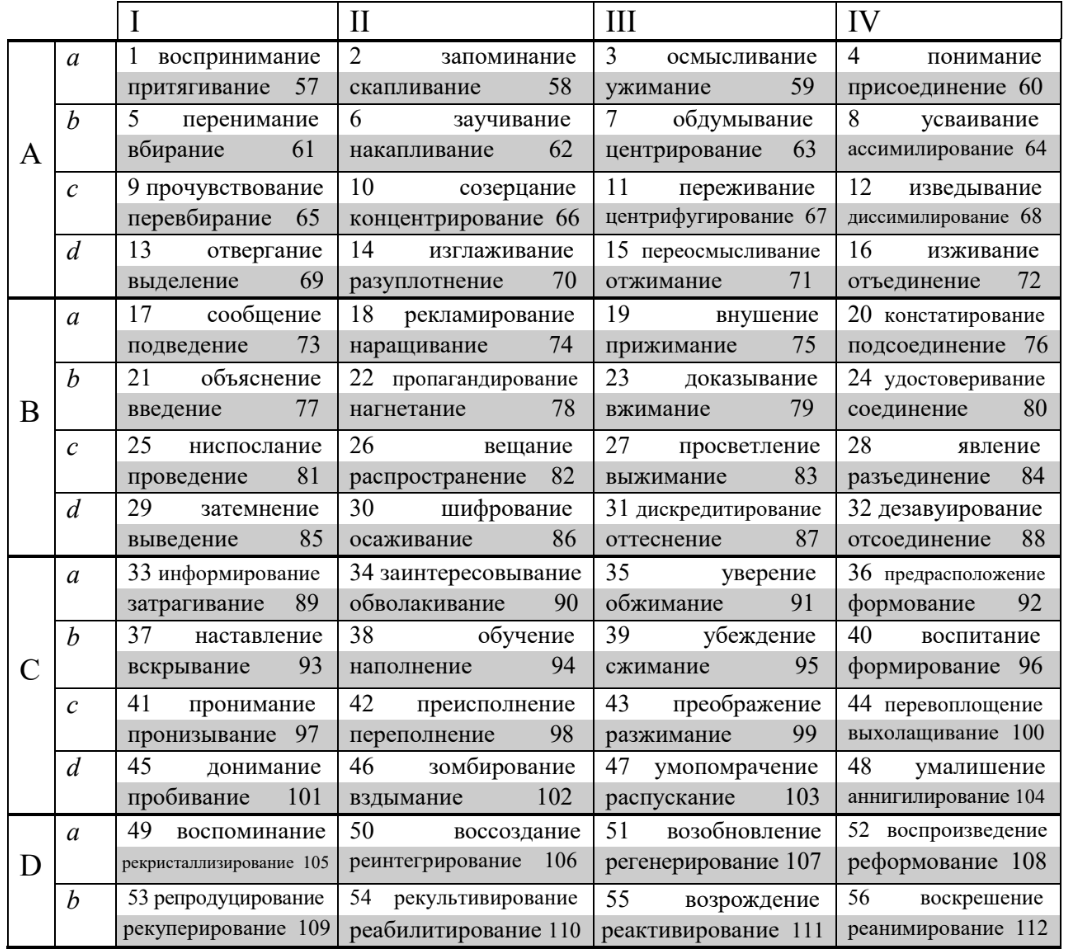
\includegraphics{Contents/part_kb/images/sd_actions/macroproc_table.png}}
    \scnrelfrom{источник}{\cite{Hardzei2017}}
    \scntext{пояснение}{На изображении представлена типология \textit{воздействий}. Любое воздействие характеризуется принадлежностью четырём классам, соответствующим признакам классификации. Заштрихованы \textit{физические воздействия}.}
   
    \scnheader{Специфицируемые классы воздействий}
    \begin{scnhassubset}
            \scnitem{формование}
            \begin{scnindent}
	            \begin{scnreltoset}{пересечение}
	                \scnitem{воздействие трансформации}
	                \scnitem{воздействие среда-оболочка}
	                \scnitem{воздействие генерации}
	                \scnitem{физическое воздействие}
	            \end{scnreltoset}
        	\end{scnindent}
            \scnitem{притягивание}
            \begin{scnindent}
	            \begin{scnreltoset}{пересечение}
	                \scnitem{воздействие активизации}
	                \scnitem{воздействие среда-оболочка}
	                \scnitem{воздействие инициации}
	                \scnitem{физическое воздействие}
	            \end{scnreltoset}
        	\end{scnindent}
            \scnitem{выхолащивание}
            \begin{scnindent}
	            \begin{scnreltoset}{пересечение}
	                \scnitem{воздействие трансформации}
	                \scnitem{воздействие ядро-оболочка}
	                \scnitem{воздействие генерации}
	                \scnitem{физическое воздействие}
	            \end{scnreltoset}
        	\end{scnindent}
            \scnitem{аннигилирование}
            \begin{scnindent}
	            \begin{scnreltoset}{пересечение}
	                \scnitem{воздействие трансформации}
	                \scnitem{воздействие оболочка-среда}
	                \scnitem{воздействие генерации}
	                \scnitem{физическое воздействие}
	            \end{scnreltoset}
        	\end{scnindent}
            \scnitem{введение}
            \begin{scnindent}
	            \begin{scnreltoset}{пересечение}
	                \scnitem{воздействие эксплуатации}
	                \scnitem{воздействие оболочка-ядро}
	                \scnitem{воздействие инициации}
	                \scnitem{физическое воздействие}
	            \end{scnreltoset}
        	\end{scnindent}
            \scnitem{распускание}
            \begin{scnindent}
	            \begin{scnreltoset}{пересечение}
	                \scnitem{воздействие трансформации}
	                \scnitem{воздействие оболочка-среда}
	                \scnitem{воздействие амплификации}
	                \scnitem{физическое воздействие}
	            \end{scnreltoset}
        	\end{scnindent}
            \scnitem{разжимание}
            \begin{scnindent}
	            \begin{scnreltoset}{пересечение}
	                \scnitem{воздействие трансформации}
	                \scnitem{воздействие ядро-оболочка}
	                \scnitem{воздействие амплификации}
	                \scnitem{физическое воздействие}
	            \end{scnreltoset}
        	\end{scnindent}
            \scnitem{разъединение}
            \begin{scnindent}
	            \begin{scnreltoset}{пересечение}
	                \scnitem{воздействие эксплуатации}
	                \scnitem{воздействие ядро-оболочка}
	                \scnitem{воздействие генерации}
	                \scnitem{физическое воздействие}
	            \end{scnreltoset}
        	\end{scnindent}
    \end{scnhassubset}
    
    \scnheader{Пример sc.g-текста, описывающего спецификацию воздействия}
    \scneq{\scnfileimage[40em]{Contents/part_kb/images/sd_actions/tapaz_description_example.png}}
    \scniselement{sc.g-текст}
    \scntext{пояснение}{Представленный фрагмент базы знаний содержит декомпозицию воздействия во времени, указание принадлежности данного декомпозируемого воздействия и полученных в результате данной декомпозиции воздействий определенному их классу из приведенной выше классификации, а также указание участников данных акций.}
    \scntext{пояснение}{Представленный фрагмент базы знаний можно протранслировать в следующий текст естественного языка: <<Некто принимает молоко, затем окисляет молоко, а именно: нормализует молоко до 15-процентной жирности, затем очищает молоко, затем пастеризует молоко, затем охлаждает молоко до определённой температуры, затем вносит закваску в молоко, затем сквашивает молоко, затем режет сгусток, затем подогревает сгусток, затем обрабатывает сгусток, затем отделяет сыворотку, затем охлаждает сгусток и, в итоге, производит творог>>.}
    
    \scnheader{субъект}
    \scnidtftext{часто используемый sc-идентификатор}{индивид}
    \scnidtf{активная сущность}
    \scnidtf{сущность, способная самостоятельно выполнять некоторые виды действий}
    \scnidtf{агент деятельности}
    \scnsuperset{Собственное Я}
    \scnsuperset{внутренний субъект ostis-системы}
    \scnsuperset{внешний субъект ostis-системы, с которым осуществляется взаимодействие}
    \scnsuperset{внешний субъект ostis-системы, с которым взаимодействие не происходит}
    \scnheader{внутренний субъект ostis-системы}
    \scnidtf{субъект, входящий в состав той \textit{ostis-системы, в базе знаний} которой он описывается}
    \scnsuperset{sc-агент}
    \scntext{пояснение}{Под \textit{внутренним субъектом ostis-системы} понимается такой \textit{субъект}, который выполняет некоторые \textit{действия} в \uline{той же памяти}, в которой хранится его знак.\\
        К числу \textit{внутренних субъектов ostis-системы} относятся входящие в нее \textit{sc-агенты}, частные sc-машины, целые интеллектуальные подсистемы.}
    
    \scnheader{внешний субъект ostis-системы, с которым осуществляется взаимодействие}
    \scntext{пояснение}{К числу \textit{внешних субъектов ostis-системы, с которыми осуществляется взаимодействие}, относятся конечные пользователи \textit{ostis-системы}, ее разработчики, а также другие компьютерные системы(причем не только интеллектуальные).}
    
    \scnheader{субъект действия\scnrolesign}
    \scnsubset{субъект\scnrolesign}
    \scnidtf{сущность, воздействующая на некоторую другую сущность в процессе заданного действия\scnrolesign}
    \scnidtf{сущность, создающая \textit{причину} изменений другой сущности (объекта действия)\scnrolesign}
    \scnidtf{быть субъектом данного действия\scnrolesign}
    \scnsuperset{субъект неосознанного воздействия\scnrolesign}
    \scnsuperset{субъект осознанного воздействия\scnrolesign}
	\begin{scnindent}
	    \scnidtf{субъект целенаправленного, активного воздействия\scnrolesign}
	\end{scnindent}
    
    \scnheader{исполнитель*}
    \scntext{пояснение}{Связки отношения \textit{исполнитель*} связывают \textit{sc-элементы}, обозначающие \textit{действие} и \textit{sc-элементы}, обозначающие \textit{субъекта}, который предположительно будет осуществлять, осуществляет или осуществлял выполнение указанного \textit{действия}. Данное отношение может быть использовано при назначении конкретного исполнителя для проектной задачи по развитию баз знаний.\\
        В случае, когда заранее неизвестно, какой именно \textit{субъект*} будет исполнителем данного \textit{действия}, отношение \textit{исполнитель*} может отсутствовать в первоначальной формулировке \textit{задачи} и добавляться позже, уже непосредственно при исполнении.\\
        Когда действие выполняется (является \textit{настоящей сущностью}) или уже выполнено (является \textit{прошлой сущностью}), то исполнитель этого действия в каждый момент времени уже определён. Но когда действие только инициировано, тогда важно знать:
        \begin{enumerate}
            \item кто \uline{хочет} выполнить это действие и насколько важно для него стать исполнителем данного действия;
            \item кто \uline{может} выполнить данное действие и каков уровень его квалификации и опыта;
            \item кто и кому поручает выполнить это действие и каков уровень ответственности за невыполнение (приказ, заказ, официальный договор, просьба...)
        \end{enumerate}
        При этом следует помнить, что связь отношения \textit{исполнитель*} в данном случае также является временной прогнозируемой сущностью.\\
        Первым компонентом связок отношений \textit{исполнитель*} является знак \textit{действия}, вторым --- знак \textit{субъекта} исполнителя}
        
    \scnheader{объект воздействия\scnrolesign}
    \scnsubset{объект\scnrolesign}
    \scnidtf{сущность, на которую осуществляется воздействие в рамках заданного действия\scnrolesign}
    \scnidtf{сущность, являющаяся в рамках заданного действия исходным условием (аргументом), необходимым для выполнения этого действия\scnrolesign}
    \scntext{примечание}{Для разных действий количество объектов действий может быть различным.}
    \scntext{примечание}{Поскольку действие является процессом и, соответственно, представляет собой \textit{динамическую структуру}, то и знак \textit{субъекта действия\scnrolesign}, и знак \textit{объекта действия\scnrolesign} являются элементами данной структуры. В связи с этим можно рассматривать отношения \textit{субъект действия\scnrolesign} и \textit{объект действия\scnrolesign} как \textit{ролевые отношения}. Данный факт не  запрещает вводить аналогичные \textit{неролевые отношения}, однако это нецелесообразно.}
    
    \scnheader{продукт\scnrolesign}
    \scnidtf{быть продуктом заданного действия\scnrolesign}
    \scnsubset{продукт*}
    \scnsubset{результат*}
    \scnidtf{сухой остаток\scnrolesign}
    \scnidtf{то, ради чего может быть выполнено, выполняется или будет выполняться заданное действие\scnrolesign}
    \scntext{примечание}{Продуктом действия может быть некоторая материальная сущность, некоторое множество (тираж) одинаковых материальных сущностей, некоторая информационная конструкция}
    
    \scnheader{результат*}
    \scntext{пояснение}{Связки отношения \textit{результат*} связывают \textit{sc-элемент}, обозначающий \textit{действие}, и \textit{sc-конструкцию}, описывающую результат выполнения рассматриваемого действия, другими словами, цель, которая должна быть достигнута при выполнении \textit{действия}.\\
    Результат может специфицироваться как атомарным высказыванием, так и неатомарным, т.е. конъюнктивным, дизъюнктивным, строго дизъюнктивным и т.д.\\
    В случае, когда успешное выполнение \textit{действия} приводит к изменению какой-либо конструкции в \textit{\mbox{sc-памяти}}, которое необходимо занести в историю изменений базы знаний или использовать для демонстрации протокола решении задачи, генерируется соответствующая связка отношения \textit{результат*}, связывающая задачу и \textit{sc-конструкцию}, описывающую данное изменение. Конкретный вид указанной \textit{\mbox{sc-конструкции}} зависит от типа действия.}
    \scnrelboth{следует отличать}{цель*}
	\begin{scnindent}
	    \scnidtf{спецификация планируемого результата*}
	    \scntext{примечание}{Следует также отмечать то, что является непосредственно результатом (продуктом) некоторого действия, и то, что является предварительной (исходной, стартовой) спецификацией этого результата. Далеко не всегда результатом действия является именно то, что планировалось (было целью) изначально.}
	\end{scnindent}
    
    \scnheader{класс выполняемых действий*}
    \scnidtf{класс действий, выполняемых классом субъектов*}
    \scntext{пояснение}{Связки отношения \textit{класс выполняемых действий*} связывают классы \textit{субъектов} и классы действий, при этом предполагается, что каждый субъект указанного класса способен выполнять действия указанного класса действий.}
    
    \scnheader{заказчик*}
    \scntext{пояснение}{Связки отношения \textit{заказчик*} связывают классы \textit{sc-элементы}, обозначающие \textit{действие}, и \textit{sc-элементы}, обозначающие \textit{субъекта}, который заинтересован в выполнении данного действия и, как правило, инициирует его выполнение. Данное отношение может быть использовано при указании того, кто поставил проектную задачу по развитию баз знаний.\\
        Первым компонентов связок отношения \textit{заказчик*} является знак \textit{действия}, вторым --- знак \textit{субъекта}.}
    
    \scnheader{инициатор*}
    \scntext{пояснение}{Связки отношения \textit{инициатор*} связывают \textit{sc-элемент}, обозначающий \textit{инициированное действие}, и знак \textit{субъекта}, который является инициатором данного \textit{действия}, то есть \textit{субъектом}, который инициировал данное \textit{действие} и, как правило, заинтересован в его успешном выполнении.}
    
    \scnheader{объект\scnrolesign}
    \scnidtf{аргумент действия\scnrolesign}
    \scntext{пояснение}{Связки отношения \textit{объект\scnrolesign} связывают \textit{sc-элемент}, обозначающий \textit{действие}, и знак той сущности, над которой (по отношению к которой) осуществляется данное \textit{действие}, и, например, знак \textit{структуры}, подлежащий верификации.}
    \scnsuperset{первый аргумент действия\scnrolesign}
    \scnsuperset{второй аргумент действия\scnrolesign}
    \scnsuperset{третий аргумент действия\scnrolesign}
    
    \scnheader{класс аргументов*}
    \scnidtf{класс аргументов класса команд*}
    \scnidtf{быть классом sc-элементов, экземпляры которого являются аргументами для заданного класса команд*}
    \scnsuperset{класс первых аргументов*}
    \scnsuperset{класс вторых аргументов*}
    \scntext{пояснение}{Связки отношения \textit{класс аргументов*} связывают \textit{классы команд} (подмножества множества \textit{команд}) и классы \textit{sc-элементов}, которые могут быть аргументами действий, соответствующих данному \textit{классу команд}. В случае, когда \textit{команды} данного класса имеют один аргумент, используется собственно отношение  \textit{класс аргументов*}, в случае, когда команды данного класса имеют более одного аргумента, то используются подмножества данного отношения, такие как \textit{класс первых аргументов*}, \textit{класс вторых аргументов*} и т.д.\\
        Если для некоторого \textit{класса команд} не указан тип какого-либо из аргументов, то предполагается, что в качестве данного аргумента может выступать любой \textit{sc-элемент}.\\
        Первым компонентом связок отношения \textit{класс аргументов*} является знак \textit{класса команд}, вторым --- знак класса \textit{sc-элемента}, которые могут быть \textit{аргументами действий\scnrolesign}, соответствующих данному \textit{классу команд}.}
    
        \bigskip
\end{scnsubstruct}
\scnendsegmentcomment{Предметная область и онтология субъектно-объектных спецификаций воздействий}

        \begin{SCn}
    \scnsegmentheader{Уточнение понятий план сложного действия, классы действий, класса задач, метода}
    \begin{scnsubstruct}
        \scniselement{сегмент базы знаний}
        
        \scnheader{план сложного действия}
        \scnidtf{план}
        \scnidtf{план выполнения сложного действия}
        \scnidtf{план решения \textit{сложной задачи}}
        \scnidtf{план выполнения действия}
        \scnidtf{спецификация выполнения действия}
        \scnidtf{декомпозиция выполняемого действия на систему последовательно/параллельно выполняемых поддействий*}
        \scnidtf{описание того, как может быть выполнено соответствующее сложное действие}
        \scnidtf{спецификация соответствующего действия, уточняющая то, \uline{как} предполагается выполнять это действие}
        \scnidtf{план решения задачи (выполнения сложного действия) путем описания последовательности выполнения поддействий с описанием того, как передается управление от одних поддействий другим, как осуществляется распараллеливание, как организуется выполнение циклов}
        \scntext{определение}{вид спецификации \textit{сложного действия}, представляющий собой систему \textit{задач}, \textit{интерпретация} которой (предполагающая решение указанных \textit{задач} в определенной последовательности) обеспечивает выполнение специфицируемого \textit{сложного действия}}
        \scnsubset{знание}
        \scntext{пояснение}{Каждый \textit{план} представляет собой \textit{семантическую окрестность, ключевым sc-элементом\scnrolesign} является \textit{действие}, для которого дополнительно детализируется предполагаемый процесс его выполнения. Основная задача такой детализации --- локализация области базы знаний, в которой предполагается работать, а также набора агентов, необходимого для выполнения  описываемого действия. При этом детализация не обязательно должна быть доведена до уровня элементарных действий, цель составления плана --- уточнение подхода к решению той или иной задачи, не всегда предполагающее составления подробного пошагового решения.\\
            При описании \textit{плана} может быть использован как процедурный, так и декларативный подход. В случае процедурного подхода для соответствующего \textit{действия} указывает его декомпозиция на более частные поддействия, а также необходимая спецификация этих поддействий. В случае декларативного подхода указывается набор подцелей (например, при помощи логических утверждений), достижение которых необходимо для выполнения рассматриваемого \textit{действия}. На практике оба рассмотренных подхода можно комбинировать.\\
            В общем случае \textit{план} может содержать и переменные, например в случае, когда часть плана задается в виде цикла (многократного повторения некоторого набора действий). Также план может содержать константы, значение которых в настоящий момент не установлено и станет известно, например, только после выполнения предшествующих ему \textit{действий}.\\
            Каждый \textit{план} может быть задан заранее как часть спецификации \textit{действия}, т.е. \textit{задачи}, а может формироваться \textit{субъектов} уже собственно в процессе выполнения \textit{действия}, например, в случае использования стратегии разбиения задачи над подзадачи. В первом случае \textit{план} \textit{включается*} в \textit{задачу}, соответствующую тому же действию.}
        \begin{scnsubdividing}
            \scnitem{процедурный план сложного действия}
        	\begin{scnindent}
                \scnidtf{декомпозиция \textit{сложного действия} на множество последовательно и/или параллельно выполняемых \textit{поддействий}}
            \end{scnindent}
            \scnitem{непроцедурный план сложного действия}
        	\begin{scnindent}
                \scnidtf{декомпозиция исходной \textit{задачи}, соответствующей заданному \textit{сложному действию}, на иерархическую систему и/или подзадач}
            \end{scnindent}
        \end{scnsubdividing}
        
        \scnheader{процедурный план сложного действия}
        \scntext{примечание}{В \textit{процедурном плане выполнения сложного действия} соответствующие \textit{поддействия*} декомпозируемого \textit{сложного действия} представляются специфицирующими их \textit{задачами}. Но, кроме такого рода \textit{задач}, в \textit{процедурный план выполнения сложного действия} входят также \textit{задачи}, которые специфицируют \textit{действия}, обеспечивающие:
            \begin{scnitemize}
                \item синхронизацию выполнения \textit{поддействий*} заданного \textit{сложного действия};
                \item передачу управления указанным \textit{поддействиям*} (а точнее, соответствующим им \textit{задачам}), т.е. инициирование указанных \textit{поддействий*} (и соответствующих им \textit{задач}).
            \end{scnitemize}}
        
        \scnheader{действие управления интерпретацией процедурного плана сложного действия}
        \scnrelboth{семантически близкий знак}{задача управления интерпретацией процедурного плана сложного действия}
        \scnsuperset{безусловная передача управления от одного поддействия к другому}
        \scnsuperset{инициирование заданного поддействия при возникновении в базе знаний ситуации или события заданного вида}
        \scnsuperset{инициирование заданного множества поддействий при успешном завершении выполнения \uline{всех} поддействий другого заданного множества}
        \scnsuperset{инициирование заданного множества поддействий при успешном завершении выполнения \uline{по крайней мере одного} поддействия другого заданного множества}%примечания не было
        \scntext{примечание}{Выделенные классы \textit{действий управления интерпретацией процедурного плана сложного действия} дают возможность реализовать различные виды параллелизма, если это позволяет задача.}
        
        \scnheader{класс действий}
        \scnrelto{семейство подклассов}{действие}
        \scnidtftext{пояснение}{\uline{максимальное} множество аналогичных (похожих в определенном смысле) действий, для которого существует (но не обязательно известных в текущий момент) по крайней мере один \textit{метод} (или средство), обеспечивающий выполнение \uline{любого} действия из указанного множества действий}
        \scnidtf{множество однотипных действий}
        \scnsuperset{класс элементарных действий}
        \scnsuperset{класс легковыполнимых сложных действий}
        \scntext{примечание}{Тот факт, что каждому выделяемому \textit{классу действий} соответствует по крайней мере один общий для них \textit{метод} выполнения этих \textit{действий}, означает то, что речь идет о \uline{семантической} кластеризации множества \textit{действий}, т.е. выделении \textit{классов действий} по признаку \uline{семантической близости} (сходства) \textit{действий}, входящих в состав выделяемого \textit{класса действий}. При этом прежде всего учитывается аналогичность (сходство) \textit{исходных ситуаций и целевых ситуаций} рассматриваемых \textit{действий}, т.е. аналогичность \textit{задач}, решаемых в результате выполнения соответствующих \textit{действий}. Поскольку одна и та же \textit{задача} может быть решена в результате выполнения нескольких \uline{разных} \textit{действий}, принадлежащих \uline{разным} \textit{классам действий}, следует говорить не только о \textit{классах действий} (множествах аналогичных действий), но и о \textit{классах задач} (о множествах аналогичных задач), решаемых этими \textit{действиями}. Так, например, на множестве \textit{классом действий} заданы следующие \textit{отношения}:
            \begin{scnitemize}
                \item \textit{отношение}, каждая связка которого связывает два разных (непересекающихся) \textit{класса действий}, осуществляющих решение одного и того же \textit{класса задач};
                \item \textit{отношение}, каждая связка которого связывает два разных \textit{класса действий}, осуществляющих решение разных \textit{классов задач}, один из которых является \textit{надмножеством} другого.
            \end{scnitemize}}
        \scntext{правило идентификации экземпляров}{Конкретные \textit{классы действий} в рамках \textit{Русского языка} именуются по следующим правилам:
            \begin{scnitemize}
                \item в начале идентификатора пишется слово ``\textit{действие}'' и ставится точка;
                \item далее со строчной буквы идет либо содержащее глагол совершенного вида в инфинитиве описание сути того, что требуется получить в результате выполнения действий данного класса, либо вопросительное предложение, являющееся спецификацией запрашиваемой (ответной) информации.
            \end{scnitemize}
            Например:\\
            \textit{действие, сформировать полную семантическую окрестность указываемой сущности\\
                действие, верифицировать заданную структуру}Допускается использовать менее строгие идентификаторы, которые, однако, обязаны оперировать словом ``\textit{действие}'' и достаточно четко специфицировать суть действий описываемого класса.\\
                Например:\\
            \textit{действие редактирования базы знаний}\\
            \textit{действие, направленное на установление темпоральных характеристик указываемой сущности}}
            
        \scnheader{класс элементарных действий}
        \scnidtf{множество элементарных действий, указание принадлежности которому является \uline{необходимым} и достаточным условием для выполнения этого действия}
        \scntext{примечание}{Множество всевозможных элементарных действий, выполняемых каждым субъектом, должно быть \uline{разбито} на классы элементарных действий.}
        \scntext{пояснение}{Принадлежность некоторого \textit{класса действий} множеству \textit{классу элементарных действий}, фиксирует факт того, что при указании всех необходимых аргументов принадлежности \textit{действия} данному классу достаточно для того, чтобы некоторый субъект мог приступить к выполнению этого действия.\\
            При этом, даже если \textit{класс действий} принадлежит множеству \textit{класс элементарных действий}, не запрещается вводить более частные \textit{классы действий}, для которых, например, заранее фиксируется один из аргументов.\\
            Если конкретный \textit{класс элементарных действий} является более частным по отношению к \textit{действиям в sc-памяти}, то это говорит о наличии в текущей версии системы как минимум одного \textit{sc-агента}, ориентированного на выполнение действий данного класса.}
        
        \scnheader{класс легковыполнимых сложных действий}
        \scnidtf{множество сложных действий, для которого известен и доступен по крайней мере один \textit{метод}, интерпретация которого позволяет осуществить полную (окончательную, завершающуюся элементарными действиями) декомпозицию на поддействия \uline{каждого} сложного действия из указанного выше множества}
        \scnidtf{множество всех сложных действий, выполнимых с помощью известного \textit{метода}, соответствующего этому множеству}
        \scntext{пояснение}{Принадлежность некоторого \textit{класса действий} множеству \textit{класс легковыполнимых сложных действий} фиксирует факт того, что даже при указании всех необходимых аргументов принадлежности \textit{действия} данному классу недостаточно для того, чтобы некоторый \textit{субъект} приступил к выполнению этого действия, и требуются дополнительные уточнения.}
        
        \scnheader{сужение отношения по первому домену*(спецификация*;класс действий*)}
        \scnidtftext{часто используемый идентификатор}{спецификация класса действий*}
        \begin{scnsubdividing}
            \scnitem{обобщенная формулировка задач соответствующего класса*}
        	\begin{scnindent}
                \begin{scnsubdividing}
                    \scnitem{обобщенная декларативная формулировка задач соответствующего класса*}
                    \scnitem{обобщенная процедурная формулировка задач соответствующего класса*}
                \end{scnsubdividing}
            \end{scnindent}
            \scnitem{метод*}
        	\begin{scnindent}
                \scnidtf{метод решения задач заданного класса*}
                \scnidtf{метод выполнения действий соответствующего (заданного) класса*}
                \begin{scnindent}
	                \begin{scnsubdividing}
	                    \scnitem{процедурный метод выполнения действий соответствующего класса*}
	                	\begin{scnindent}
	                        \scnidtf{обобщенный план выполнения действий заданного класса*}
	                    \end{scnindent}
	                    \scnitem{декларативный метод выполнения действий соответствующего класса*}
	                	\begin{scnindent}
	                        \scnidtf{обобщенная декларативная спецификация выполнения действий заданного класса*}
	                    \end{scnindent}
	                \end{scnsubdividing}
                \end{scnindent}
            \end{scnindent}
        \end{scnsubdividing}
        
        \scnheader{класс задач}
        \scnidtf{множество аналогичных задач}
        \scnidtf{множество задач, для которого можно построить обобщенную формулировку задач, соответствующую всему этому множеству задач}
        \scntext{примечание}{Каждая \textit{обобщенная формулировка задач соответствующего класса} по сути есть не что иное, как строгое логическое определение указанного класса задач.}
        \scnrelto{семейство подмножеств}{задача}
        \scntext{правило идентификации экземпляров}{Конкретные \textit{классы задач} в рамках \textit{Русского языка} именуются по следующим правилам:
            \begin{scnitemize}
                \item в начале идентификатора пишется слово ``\textit{задача}'' и ставится точка;
                \item далее с прописной буквы идет либо содержащее глагол совершенного вида в инфинитиве описание сути того, что требуется получить в результате решения данного \textit{класса задач}, либо вопросительное предложение, являющееся спецификацией запрашиваемой (ответной) информации.
            \end{scnitemize}
            Например:\\
            \textit{задача. сформировать полную семантическую окрестность указываемой сущности}\\
            \textit{задача. верифицировать заданную структуру}Допускается использовать менее строгие идентификаторы, которые, однако, обязаны оперировать словом ``\textit{задача}'' и достаточно четко специфицировать суть задач описываемого класса.\\
            Например:\\
            \textit{задача на установление значения величины}\\
            \textit{задача на доказательство}}
            
        \scnheader{класс команд}
        \scnrelto{семейство подмножеств}{задача}
        \scnsuperset{класс интерфейсных пользовательских команд}
        \begin{scnindent}
        	\scnsuperset{класс интерфейсных команд пользователя ostis-системы}
        \end{scnindent}
        \scnsuperset{класс команд без аргументов}
        \scnsuperset{класс команд с одним аргументом}
        \scnsuperset{класс команд с двумя аргументами}
        \scnsuperset{класс команд с произвольным числом аргументов}
        \scntext{пояснение}{Идентификатор конкретного класса \textit{класса команд} в рамках \textit{Русского языка} пишется со строчной буквы и представляет собой либо содержащее глагол совершенного вида в инфинитиве описание сути того, что требуется получить в результате выполнения действий, соответствующих данному \textit{классу команд}, либо вопросительное предложение, являющееся спецификацией запрашиваемой (ответной) информации.\\ Например:\\
            \textit{сформировать полную семантическую окрестность указываемой сущности}\\
            \textit{верифицировать заданную структуру}Допускается использовать менее строгие идентификаторы, которые, однако, обязаны оперировать словом ``\textit{команда}'' и достаточно четко специфицировать суть задач описываемого класса.\\
            Например:\\
            \textit{команда редактирования базы знаний}\\
            \textit{команда установления темпоральных характеристик указываемой сущности}}
        \begin{scnsubdividing}
            \scnitem{атомарный класс команд}
            \scnitem{неатомарный класс команд}
        \end{scnsubdividing}
        
        \scnheader{атомарный класс команд}
        \scntext{пояснение}{Принадлежность некоторого \textit{класса команд} множеству \textit{атомарных классов команд} фиксирует факт того, что данная спецификация является достаточной для того, чтобы некоторый субъект приступил к выполнению соответствующего действия.\\
            При этом, даже если \textit{класса команд} принадлежит множеству \textit{атомарных классов команд} не запрещается вводить более частные \textit{классы команд}, в состав которых входит информация, дополнительно специфицирующая соответствующее \textit{действие}.\\
            Если соответствующий данному \textit{классу команд класс действий} является более частным по отношению к \textit{действиям в sc-памяти}, то попадание данного класса команд во множество \textit{атомарных классов команд} говорит о наличии в текущей версии системы как минимум одного \textit{sc-агента}, условие инициирования которого соответствует формулировке команд данного класса.}
        
        \scnheader{неатомарный класс команд}
        \scntext{пояснение}{Принадлежность некоторого \textit{класса команд} множеству \textit{неатомарных классов команд} фиксирует факт того, что данная спецификация не является достаточной для того, чтобы некоторый субъект приступил к выполнению соответствующего действия, и требует дополнительных уточнений.}
        
        \scnheader{класс действий}
        \begin{scnsubdividing}
            %TODO: check by human--->
            \scnitem{\textit{класс действий, однозначно задаваемый решаемым классом задач}}
        	\begin{scnindent}
                \scnidtf{\textit{класс действий}, обеспечивающих решение соответствующего \textit{класса задач} и использующих при этом любые, самые разные \textit{методы} решения задач этого класса}
            \end{scnindent}
            \scnitem{\textit{класс действий, однозначно задаваемый используемым методом решения задач}}
        \end{scnsubdividing}
        
        \scnheader{метод}
        \scnrelto{второй домен}{метод*}
        \scnidtf{описание того, \uline{как} может быть выполнено любое или почти любое действие, принадлежащее соответствующему классу действий}
        \scnidtf{метод решения соответствующего класса задач, обеспечивающий решение любой или большинства задач указанного класса}
        \scnidtf{обобщенная спецификация выполнения действий соответствующего класса}
        \scnidtf{обобщенная спецификация решения задач соответствующего класса}
        \scnidtf{программа решения задач соответствующего класса, которая может быть как процедурной, так и декларативной (непроцедурной)}
        \scnidtf{знание о том, как можно решать задачи соответствующего класса}
        \scnsubset{знание}
        \scniselement{вид знаний}
        \scnidtf{способ}
        \scnidtf{знание о том, как надо решать задачи соответствующего класса задач (множества эквивалентных (однотипных, похожих) задач)}
        \scnidtf{метод (способ) решения некоторого (соответствующего) класса задач}
        \scnidtf{информация (знание), достаточная для того, чтобы решить любую \textit{задачу}, принадлежащую соответствующему \textit{классу задач} с помощью соответствующей \textit{модели решения задач}}
        \scnidtf{обобщенный план выполнения некоторого класса сложных действий (или обобщенный план решения соответствующего класса сложных задач), привязка которого к конкретной задаче указанного класса и последующая интерпретация обеспечивает решение любой или почти любой задачи этого класса}
        \scntext{примечание}{Очевидно, что трудоемкость разработки метода определяется не столько мощностью класса задач, решаемых с помощью разрабатываемого метода, сколько их семантической близостью, аналогичностью.}
        \scnidtf{метод решения соответствующего класса задач}
        \scnidtf{метод выполнения соответствующего класса действий}
        \scnidtf{пассивный метод, хранимый в базе знаний и используемый соответствующими коллективами агентов при соответствующем их инициировании}
        \scnidtf{метод выполнения действий некоторого класса или метод решения задач некоторого класса или метод, который может быть использован для выполнения некоторого конкретного действия или для решения некоторой конкретной задачи}
        \scnidtf{обобщенное описание того, как можно выполнить действия из соответствующего класса действий или как можно решить задачу из соответствующего класса задач}
        \scnsuperset{метод сведения задач к подзадачам}
        \begin{scnindent}
        	\scnidtf{класс логически эквивалентных методов, обеспечивающих решение задач путем сведения этих задач к подзадачам и отличающихся только деталями формализации}
        \end{scnindent}
        \scntext{примечание}{В состав спецификации каждого \textit{класса задач} входит описание способа привязки \textit{метода} к исходным данным конкретной \textit{задачи}, решаемой с помощью этого \textit{метода}. Описание такого способа привязки включает в себя:
            \begin{scnitemize}
                \item набор переменных, которые входят как в состав \textit{метода}, так и в состав \textit{обобщенной формулировки задач соответствующего класса} и значениями которых являются соответствующие элементы исходных данных каждой конкретной решаемой задачи;
                \item часть \textit{обобщенной формулировки задач} того класса, которому соответствует рассматриваемый \textit{метод}, являющихся описанием \uline{условия применения} этого \textit{метода}.
            \end{scnitemize}
            \bigskip
            Сама рассматриваемая привязка \textit{метода} к конкретной \textit{задаче}, решаемой с помощью этого \textit{метода} осуществляется путем \uline{поиска} в \textit{базе знаний} такого фрагмента, который удовлетворяет условиям применения указанного \textit{метода}. Одним из результатов такого поиска и является установление соответствия между указанными выше переменными используемого \textit{метода} и значениями этих переменных в рамках конкретной решаемой \textit{задачи}.\\
            Другим вариантом установления рассматриваемого соответствия является явное обращение (вызов, call) соответствующего \textit{метода} (программы) с явной передачей соответствующих параметров. Но такое не всегда возможно, т.к. при выполнении процесса решения конкретной \textit{задачи} на основе декларативной спецификации выполнения этого действия нет возможности установить:
            \begin{scnitemize}
                \item когда необходимо инициировать вызов (использование) требуемого \textit{метода};
                \item какой конкретно \textit{метод} необходимо использовать;
                \item какие параметры, соответствующие конкретной инициируемой \textit{задаче}, необходимо передать для привязки используемого \textit{метода} к этой \textit{задаче}.
            \end{scnitemize}
            Процесс привязки \textit{метода} решения \textit{задач} к конкретной \textit{задаче}, решаемой с помощью этого \textit{метода}, можно также представить как процесс, состоящий из следующих этапов:
            \begin{scnitemize}
                \item построение копии используемого \textit{метода};
                \item склеивание основных (ключевых) переменных используемого \textit{метода} с основными параметрами конкретной решаемой \textit{задачи}.
            \end{scnitemize}
            В результате этого на основе рассматриваемого \textit{метода} используемого в качестве образца (шаблона) строится спецификация процесса решения конкретной задачи --- процедурная спецификация (\textit{план}) или декларативная.}
        \scntext{примечание}{Заметим, что \textit{методы} могут использоваться даже при построении \textit{планов} решения конкретных \textit{задач}, в случае, когда возникает необходимость многократного повторения неких цепочек \textit{действий} при априори неизвестном количестве таких повторений. Речь идет о различного вида \textit{циклах}, которые являются простейшим видом процедурных \textit{методов} решения задач, многократно используемых (повторяемых) при реализации \textit{планов} решения некоторых \textit{задач}.}
        \scnidtf{программа}
        \scnidtf{программа выполнения действий некоторого класса}
        \scntext{примечание}{Одному \textit{классу действий} может соответствовать несколько \textit{методов} (программ).}
        \scnsuperset{программа в sc-памяти}
        \scnsuperset{процедурная программа}
        \begin{scnindent}
	        \scnidtf{обобщенный процедурный план}
	        \scnidtf{обобщенный процедурный план выполнения некоторого класса действий}
	        \scnidtf{обобщенный процедурный план решения некоторого класса задач}
	        \scnidtf{обобщенная спецификация декомпозиции любого действия, принадлежащего заданному классу действий}
	        \scnidtf{знание о некотором классе действий (и соответствующем классе задач), позволяющее для каждого из указанных действий достаточно легко построить процедурный план его выполнения}
	        \scnsubset{алгоритм}
	        \scntext{пояснение}{Каждая \textit{процедурная программа} представляет собой обобщенный процедурный план выполнения \textit{действий}, принадлежащих некоторому классу, то есть \textit{семантическую окрестность, ключевым sc-элементом\scnrolesign} является \textit{класс действий}, для элементов которого дополнительно детализируется процесс их выполнения.\\
                В остальном описание \textit{процедурной программы} аналогично описанию \textit{плана} выполнения конкретного \textit{действия} из рассматриваемого \textit{класса действий}.\\
                Входным параметрам \textit{процедурной программы} в традиционном понимании соответствуют аргументы, соответствующие каждому \textit{действию} из \textit{класса действий}, описываемого \textit{процедурной программой}. При генерации на основе \textit{процедурной программы} \textit{плана} выполнения конкретного \textit{действия} из данного класса эти аргументы принимают конкретные значения.\\
                Каждая \textit{процедурная программа} представляет собой систему описанных действий с дополнительным указанием для действия:
	            \begin{scnitemize}
	                \item либо \textit{последовательности выполнения действий*} (передачи инициирования), когда условием выполнения (инициирования) действий является завершение выполнения одного из указанных или всех указанных действий;
	                \item либо события в базе знаний или внешней среде, являющегося условием его инициирования;
	                \item либо ситуации в базе знаний или внешней среде, являющейся условием его инициирования;
	            \end{scnitemize}}
         \end{scnindent}
            %не было в стандарте \начало
	     \scnsuperset{программа sc-агента}
	     \begin{scnindent}
		     \scnidtf{метод, которому однозначно соответствует некоторыйsc-агент, способный выполнять действия, принадлежащие соответствующему данному методу классу действий}
		     \scntext{примечание}{Частным случаем метода является \textit{программа sc-агента}, в этом случае в качестве \textit{операционной семантики метода} выступает коллектив \textit{sc-агентов} более низкого уровня, интерпретирующий соответствующую программу (в предельном случае это будут \textit{sc-агенты}, являющиеся частью \textit{платформы интерпретации sc-моделей компьютерных систем}, в том числе аппаратной).Таким образом:
		         \begin{scnitemize}
		             \item можно говорить об иерархии \textit{методов} и о \textit{методах} интерпретации других \textit{методов};
		             \item можно сказать, что понятие метода обобщает понятие \textit{программы sc-агента} для \textit{неатомарных sc-агентов}.
		         \end{scnitemize}}
	     \end{scnindent}
            %%%%% \конец
	     \scntext{примечание}{Отметим, что понятие \textit{метода} фактически позволяет локализовать область решения задач соответствующего класса, то есть ограничить множество знаний, которых достаточно для решения задач данного класса определенным способом. Это, в свою очередь, позволяет повысить эффективность работы системы в целом, исключая число лишних действий.}
	     \scntext{примечание}{Каждый конкретный метод рассматривается нами как важный вид спецификации соответствующего класса задач, но также и как \textit{объект}, который и сам нуждается в спецификации, обеспечивающей непосредственное применение этого метода. Другими словами, метод является не только спецификацией (спецификацией соответствующего класса задач), но и \uline{объектом} спецификации.}
        
        %не было в стандарте \начало
        \scnheader{следует отличать*}
        \begin{scnhaselementset}
            \scnitem{план сложного действия}
            \scnitem{метод}
        \end{scnhaselementset}
        \scntext{примечание}{В отличие от \textit{метода}, \textit{план сложного действия} описывает не \textit{класс действий}, а конкретное \textit{действие}, возможно с учетом особенностей его выполнения в текущем контексте.}
         %не было в стандарте \конец
         
        \scnheader{эквивалентность задач*}
        \scnidtf{быть эквивалентной задачей*}
        \scniselement{отношение}
        \scntext{определение}{Задачи являются эквивалентными в том и только в том случае, если они могут быть решены путем интерпретации одного и того же \textit{метода} (способа), хранимого в памяти кибернетической системы.}
        \scntext{примечание}{Некоторые \textit{задачи} могут быть решены разными \textit{методами}, один из которых, например, является обобщением другого.}
        
        \scnheader{отношение, заданное на множестве*(метод)}
        \scnhaselement{подметод*}
        \begin{scnindent}
	        \scnidtf{подпрограмма*}
	        \scnidtf{быть методом, использование которого (обращение к которому) предполагается при реализации заданного метода*}
	        \scnrelboth{следует отличать}{частный метод*}
	        \begin{scnindent}
	        	\scnidtf{быть методом, обеспечивающим решение класса задач, который является подклассом задач, решаемых с помощью заданного метода*}
	        \end{scnindent}
        \end{scnindent}
        	
        \scnheader{стратегия решения задач}
        \scnsubset{метод}
        \scnidtf{метаметод решения задач, обеспечивающий либо поиск одного релевантного известного метода, либо синтез целенаправленной последовательности акций применения в общем случае различных известных методов}
        \scntext{примечание}{Можно говорить об универсальном метаметоде (универсальной стратегии) решения задач, объясняющем всевозможные частные стратегии.}
        \scntext{пояснение}{Можно говорить о нескольких глобальных \textit{стратегиях решения информационных задач} в базах знаний. Пусть в базе знаний появился знак инициированного действия с формулировкой соответствующей информационной цели, т.е. цели, направленной только на изменение состояния базы знаний. И пусть текущее состояние базы знаний не содержит контекста (исходных данных), достаточного для достижения указанной выше цели, т.е такого контекста, для которого в доступном пакете (наборе) методов (программ) имеется метод (программа), использование которого позволяет достигнуть указанную выше цель. Для достижения такой цели, контекст (исходные данные) которой недостаточен, существует три подхода (три стратегии):
            \begin{scnitemize}
                \item декомпозиция (сведение изначальной цели к иерархической системе и/или подцелей (и/или подзадач) на основе анализа текущего состояния базы знаний и анализа того, чего в базе знаний не хватает для использования того или иного метода.) При этом наибольшее внимание уделяется методам, для создания условий использования которых требуется меньше усилий. В конечном счете мы должны дойти (на самом нижнем уровне иерархии) до подцелей, контекст которых достаточен для применения одного из имеющихся методов (программ) решения задач;
                \item генерация новых знаний в семантической окрестности формулировки изначальной цели с помощью \uline{любых} доступных методов в надежде получить такое состояние базы знаний, которое будет содержать нужный контекст (достаточные исходные данные) для достижения изначальной цели с помощью какого-либо имеющегося метода решения задач;
                \item комбинация первого и второго подхода.
            \end{scnitemize}
            Аналогичные стратегии существуют и для поиска пути решения задач, решаемых во внешней среде.}
            
        \scnheader{сужение отношения по первому домену(спецификация*, метод)}
        \scnidtf{спецификация метода*}
        \begin{scnsubdividing}
            \scnitem{денотационная семантика метода*}
        	\begin{scnindent}
                \scnidtf{обобщенная формулировка класса задач, решаемых с помощью данного метода*}
                \scnrelboth{семантически близкий знак*}{обобщенная формулировка задач соответствующего класса*}
                \begin{scnindent}
                	\scntext{примечание}{Данное отношение связывает обобщенную формулировку задач не с методом, а с классом задач}
                \end{scnindent}
            \end{scnindent}
            \scnitem{операционная семантика метода*}
        	\begin{scnindent}
                \scnidtf{перечень обобщенных агентов, обеспечивающих интерпретацию метода*}
                \scnidtf{семейство методов интерпретации данного метода*}
                \scnidtf{формальное описание интерпретатора заданного метода*}
            \end{scnindent}
        \end{scnsubdividing}
        \bigskip
    \end{scnsubstruct}
    \scnendsegmentcomment{Уточнение понятий план сложного действия, классы действий, класса задач, метода}
\end{SCn}

        \begin{SCn}
    \scnsegmentheader{Уточнение понятия навыка, понятия класса методов и понятия модели решения задач}
    \begin{scnsubstruct}
        \scniselement{сегмент базы знаний}
        
        \scnheader{навык}
        \scnidtf{умение}
        \scnidtf{объединение \textit{метода} с его исчерпывающей спецификацией --- \textit{полным представлением операционной семантики метода}}
        \scnidtf{метод, интерпретация (выполнение, использование) которого полностью может быть осуществлено данной кибернетической системой, в памяти которой указанный метод хранится}
        \scnidtf{метод, который данная кибернетическая система умеет (может) применять}
        \scnidtf{метод + метод его интерпретации}
        \scnidtf{умение решать соответствующий класс эквивалентных задач}
        \scnidtf{метод плюс его операционная семантика, описывающая то, как интерпретируется (выполняется, реализуется) этот метод, и являющаяся одновременно операционной семантикой соответствующей модели решения задач}
        \begin{scnsubdividing}
            \scnitem{активный навык}
            \begin{scnindent}
                \scnidtf{самоинициирующийся навык}
            \end{scnindent}
            \scnitem{пассивный навык}
        \end{scnsubdividing}
        \scntext{пояснение}{\textit{Навыки} могут быть \textit{пассивными навыками}, то есть такими \textit{навыками}, применение которых должно явно инициироваться каким-либо агентом, либо \textit{активными навыками}, которые инициируются самостоятельно при возникновении соответствующей ситуации в базе знаний. Для этого в состав \textit{активного навыка} помимо \textit{метода} и его операционной семантики включается также \textit{sc-агент}, который реагирует на появление соответствующей ситуации в базе знаний и инициирует интерпретацию \textit{метода} данного \textit{навыка}.\\
            Такое разделение позволяет реализовать и комбинировать различные подходы к решению задач, в частности, \textit{пассивные навыки} можно рассматривать в качестве способа реализации концепции интеллектуального пакета программ.}
        
        \scnheader{класс методов}
        \scnrelto{семейство подклассов}{метод}
        \scnidtf{множество методов, для которых можно \uline{унифицировать} представление (спецификацию) этих методов}
        \scnidtf{множество всевозможных методов решения задач, имеющих общий язык представления этих методов}
        \scnidtf{множество всевозможных методов, представленных на данном языке}
        \scnidtf{множество методов, для которых задан язык представления этих методов}
        \scnhaselement{процедурный метод решения задач}
        \begin{scnindent}
        	\scnsuperset{алгоритмический метод решения задач}
        \end{scnindent}
        \scnhaselement{логический метод решения задач}
        \begin{scnindent}
        	\scnsuperset{продукционный метод решения задач}
        	\scnsuperset{функциональный метод решения задач}
        \end{scnindent}
        \scnhaselement{искусственная нейронная сеть}
        \begin{scnindent}
        	\scnidtf{класс методов решения задач на основе искусственных нейронных сетей}
        \end{scnindent}
        \scnhaselement{генетический алгоритм}
        \scnidtf{множество методов основанных на общей онтологии}
        \scnidtf{множество методов, представленных на одинаковом языке}
        \scnidtf{множество методов решений задач, которому соответсвует специальный язык (например, sc-язык), обеспечивающий представление методов из этого множества}
        \scnidtf{множество методов, которому ставится в соответствие отдельная модель решения задач}
        
        \scnheader{язык представления методов}
        \scnidtf{язык методов}
        \scnidtf{язык представления методов, соответствующих определенному классу методов}
        \begin{scnindent}
        	\scntext{примечание}{Таких специализированных языков может быть выделено целое множество, каждому из которых будет соответствовать своя модель решения задач (т.е. свой интерпретатор)}
        \end{scnindent}
        \scnidtf{язык (например sc-язык) представлений методов соответствующего класса методов}
        \scnsubset{язык}
        \scnidtf{язык программирования}
        \scnsuperset{язык представления методов обработки информации}
        \begin{scnindent}
	        \scnidtf{язык программирования внутренних действий кибернетической системы, выполняемых в их памяти}
	        \scnidtf{язык представления методов решения задач в памяти кибернетических систем}
	    \end{scnindent}
        \scnsuperset{язык представления методов решения задач во внешней среде кибернетических систем}
        \begin{scnindent}
        	\scnidtf{язык программирования внешних действий кибернетических систем}
        \end{scnindent}
        
        \scnheader{модель решения задач}
        \scnidtf{метаметод интерпретации соответствующего класса методов}
        \scnsubset{метод}
        \scnidtf{метаметод}
        \scnidtf{абстрактная машина интерпретации соответствующего класса методов}
        \scnidtf{иерархическая система микропрограмм, обеспечивающих интерпретацию соответствующего класса методов}
        \scnsuperset{алгоритмическая модель решения задач}
        \scnsuperset{процедурная параллельная синхронная модель решения задач}
        \scnsuperset{процедурная параллельная асинхронная модель решения задач}
        \scnsuperset{продукционная модель решения задач}
        \scnsuperset{функциональная модель решения задач}
        \scnsuperset{логическая модель решения задач}
        \begin{scnindent}
	        \scnsuperset{четкая логическая модель решения задач}
	        \scnsuperset{нечеткая логическая модель решения задач}
	    \end{scnindent}
        \scnsuperset{нейросетевая модель решения задач}
        \scnsuperset{генетическая модель решения задач}
        \scntext{примечание}{Для интерпретации \uline{всех} моделей решения задач может быть использован агентно-ориентированный подход}
        \scntext{пояснение}{Каждая \textit{модель решения задач} задается:
            \begin{scnitemize}
                \item соответствующим классом методов решения задач, т.е. языком представления методов этого класса;
                \item предметной областью этого класса методов;
                \item онтологией этого класса методов (т.е. денотационной семантикой языка представления этих методов);
                \item операционной семантикой указанного класса методов.
            \end{scnitemize}}
        
        \scnheader{модель решения задач*}
        \scneq{сужение отношения по первому домену(спецификация*; класс методов)*}
        \scnidtf{спецификация \textit{класса методов}*}
        \scnidtf{спецификация \textit{языка представления методов}*}
        \begin{scnreltoset}{обобщенное объединение}
            \scnitem{синтаксис языка представления методов соответствующего класса*}
            \scnitem{денотационная семантика языка представления методов соответствующего класса*}
            \scnitem{операционная семантика языка представления методов соответствующего класса*}
        \end{scnreltoset}
        \scntext{примечание}{Каждому конкретному \textit{классу методов} взаимно однозначно соответствует \textit{язык представления методов}, принадлежащих этому (специфицируемому) \textit{классу методов}. Таким образом, спецификация каждого \textit{класса методов} сводится к спецификации соответствующего \textit{языка представления методов}, т.е. к описанию его синтаксической, денотационной семантики и операционной семантики.Примерами \textit{языков представления методов} являются все \textit{языки программирования}, которые в основном относятся к подклассу \textit{языков представления методов} --- к \textit{языкам представления методов обработки информации}. Но сейчас все большую актуальность приобретает необходимость создания эффективных формальных языков представления методов выполнения действий во внешней среде кибернетических систем. Без этого комплексная автоматизация, в частности, в промышленной сфере невозможна.}
        
        \scnheader{денотационная семантика языка представления методов соответствующего класса}
        \scnrelto{второй домен}{денотационная семантика языка представления методов соответствующего класса*}
        \scnidtf{онтология соответствующего класса методов}
        \scnidtf{денотационная семантика соответствующего класса методов}
        \scnidtf{денотационная семантика языка (sc-языка), обеспечивающего представление методов соответствующего класса}
        \scnidtf{денотационная семантика соответствующей модели решения задач}
        \scntext{примечание}{если речь идет о языке, обеспечивающем внутреннее представление методов соответствующего класса в ostis-системе, то синтаксис этого языка совпадает с синтаксисом SC-кода}
        \scnsubset{онтология}
        \scnheader{операционная семантика языка представления методов соответствующего класса}
        \scnrelto{второй домен}{операционная семантика языка представления методов соответствующего класса*}
        \scnidtf{метаметод интерпретации соответствующего класса методов}
        \scnidtf{семейство агентов, обеспечивающих интерпретацию (использования) любого метода, принадлежащего соответствующему классу методов}
        \scnidtf{операционная семантика соответствующей модели решения задач}
        
        \scnheader{язык представления обобщенных формулировок задач для различных классов задач}
        \scntext{примечание}{Поскольку каждому \textit{методу} соответствует \textit{обобщенная формулировка задач}, решаемых с помощью этого \textit{метода}, то каждому \textit{классу методов} должен соответствовать не только определенный \textit{язык представления методов}, принадлежащих указанному \textit{классу методов}, но и определенный \textit{язык представления обобщенных формулировок задач для различных классов задач}, решаемых с помощью \textit{методов}, принадлежащих указанному \textit{классу методов}.}
        \bigskip
    \end{scnsubstruct}
    
    \scnendsegmentcomment{Уточнение понятия навыка, понятия класса методов и понятия модели решения задач}
    \scnsegmentheader{Уточнение понятия деятельности, понятия вида деятельности и понятия технологии}
    \begin{scnsubstruct}
        \scniselement{сегмент базы знаний}
        \scnheader{деятельность}
        \scnidtftext{пояснение}{сложный процесс, состоящий из действий, направленных на достижение нескольких \uline{разных} целей (т.е. целей, не связанных отношением цель-подцель). При этом некоторые из указанных максимальных целей могут достигаться с помощью одного и того же метода или одного и того же (фиксированного) семейства методов}
        \scnsuperset{физическая деятельность}
        \begin{scnindent}
        	\scnidtf{деятельность по преобразованию материальных сущностей (физических объектов)}
        \end{scnindent}
        \scnsuperset{информационная деятельность}
        \begin{scnindent}
	        \scnidtf{деятельность, направленная на обработку информацию}
	        \scnidtf{умственная деятельность}
        	\scntext{примечание}{Информационная деятельность является необходимым компонентом физической деятельности, обеспечивающим принятие решений, планирование и управление физическим процессом}
        \end{scnindent}
        \scnsubset{процесс}
        \scnidtf{целостный, целенаправленный процесс \uline{поведения} (функционирования) одного субъекта или сообщества субъектов, осуществляемый на основе хорошо или не очень хорошо продуманной и согласованной \textit{технологии} в последнем случае качество деятельности определяется уровнем интеллекта единоличного или коллективного субъекта, осуществляющего этот целенаправленный процесс.}
        \scnidtf{система действий, являющаяся некоторым кластером семантически близких действий, обладающих семантической близостью, семантической связностью и семантической целостностью}
        \scnidtf{трудно выполнимая семантически целостная система действий}
        \scnidtf{кластер множества действий, определяемый семантической близостью этих действий}
        \scnidtf{система связанных между собой действий, имеющих общий контекст, общую область выполнения этих действий}
        \scntext{примечание}{В состав каждой конкретной \textit{деятельности} входят \textit{действия}, являющиеся \textit{поддействиями}* других \textit{действий}, входящих в состав этой же \textit{деятельности}. При этом для каждого \textit{действия}, входящего в состав \textit{деятельности}, все поддействия этого \textit{действия} также входят в состав этой \textit{деятельности}.\\
        В состав каждой конкретной \textit{деятельности} входят также \textit{действия}, не являющиеся \textit{поддействиями}* других \textit{действий}, входящих в состав этой же \textit{деятельности}. Такие первичные (независимые, самостоятельные, автономные) \textit{действия} для заданной \textit{деятельности} могут инициироваться \uline{извне} этой \textit{деятельности} с помощью соответствующих инициирующих эти \textit{действия ситуаций} или \textit{событий}. Примерами таких инициирующих ситуаций, порождающих соответствующие действия, являются:
            \begin{scnitemize}
                \item появление в \textit{базе знаний} каких-либо противоречий, информационных дыр, информационного мусора;
                \item появление в \textit{базе знаний} описаний (информационных моделей) каких-либо нештатных ситуаций в сложном объекте управления, на которые необходимо реагировать;
                \item появление в \textit{базе знаний} формулировок различного рода задач с явным указанием инициирования соответствующих действий, направленных на решение этих задач.
            \end{scnitemize}
            К числу указанных первичных (независимых) \textit{действий}, входящих в состав \textit{объединенной деятельности кибернетической системы}, также относятся:
            \begin{scnitemize}
                \item сложное действие, целью которого является перманентное обеспечение комплексной \textit{безопасности кибернетической системы};
                \item сложное действие, целью которого является перманентное повышение качества информации (базы знаний), хранимой в памяти \textit{кибернетической системы};
                \item сложное действие, целью которого является перманентное повышение \textit{качества решателя задач кибернетической системы};
                \item сложное действие, целью которого является перманентная поддержка высокого уровня \textit{семантической совместимости} кибернетической системы со своими партнерами.
            \end{scnitemize}}
        
        \scnheader{отношение, заданное на множестве*(деятельность)}
        \scnhaselement{субъект*}
        \begin{scnindent}
	        \scnidtf{быть субъектом заданного действия или деятельности*}
	        \scnidtf{кибернетическая система, которая в рамках заданного действия или деятельности выполняет ту или иную роль, воздействует на некий объект действия, используя тот или иной инструмент*}
        	\scniselement{отношение, заданное на множестве*(действие)}
        \end{scnindent}
        \scnhaselement{контекст*}
        \begin{scnindent}
	        \scnidtf{информационный контекст, в рамках которого осуществляется выполнение заданного действия или деятельности*}
	        \scnidtf{область исполнения действия или деятельности*}
	        \scnidtf{область действия или деятельности*}
	        \scnrelfrom{первый домен}{(действие $\cup$ деятельность)}
	        \scnidtf{совокупность знаний, достаточных для информационного обеспечения заданного действия или заданной деятельности}
	        \scniselement{отношение, заданное на множестве* (действие)}
	        \scntext{примечание}{Локализация (минимизация) \textit{контекста} заданного действия или деятельности является важнейшим подготовленным этапом, обеспечивающим существенное снижение накладных расходов при непосредственном выполнении этого \textit{действия} или \textit{деятельности}.}
	   \end{scnindent}
	   \scntext{примечание}{Чаще всего \textit{контекстом} заданного \textit{действия} или \textit{деятельности} является некоторая \textit{предметная область} вместе с соответствующей ей интегрированной (объединенной) \textit{онтологией}. Поэтому хорошо продуманная декомпозиция \textit{базы знаний} интеллектуальной компьютерной системы на иерархическую систему \textit{предметных областей} и соответствующих им \textit{онтологий} имеет важное практическое значение, существенно повышающее качество (в частности, быстродействие) \textit{решателя задач} интеллектуальной компьютерной системы благодаря априорному  разбиению множества выполняемых \textit{действий} (решаемых задач) по соответствующих им \textit{контекстам}.}
        
        \scnheader{следует отличать*}
        \begin{scnhassubset}
                \scnitem{действие}
                \begin{scnindent}
	                \scnidtf{процесс достижения конкретной цели конкретных обстоятельствах}
	                \scnidtf{процесс решения конкретной задачи в конкретных условиях}
	                \scnidtf{процесс задуманный, инициированный и осуществленный некоторым (или некоторыми) субъектами (кибернетическими системами)}
	                \scntext{примечание}{\textit{действие} (точнее, соответствующая форма участия в его выполнении) является частью (фрагментом) \textit{деятельности} всех участвующих в этом субъектов (кибернетических систем)}
                \end{scnindent}
                \scnitem{деятельность}
                \begin{scnindent}
	                \scnidtf{система действий выполняемых соответствующим субъектом (кибернетической системой) скрепленное общим контекстом и определенным набором используемых навыков и инструментов}
	                \scntext{примечание}{В отличие от \textit{действия}, \textit{деятельность} носит чаще всего перманентный характер в рамках времени существования соответствующего субъекта}
                \end{scnindent}
        \end{scnhassubset}
        
        \scnheader{деятельность кибернетической системы}
        \scnidtf{полная система действий, выполняемых соответствующей кибернетической системой}
        \scnidtf{деятельность субъекта}
        \scnidtf{система всех действий соответствующего субъекта}
        \begin{scnsubdividing}
            \scnitem{внутренняя деятельность субъекта}
            \begin{scnindent}
                \scnidtf{внутренняя деятельность соответствующего субъекта}
                \scnidtf{деятельность некоторого субъекта по обработке информации}
                \scnidtf{информационная деятельность}
            \end{scnindent}
            \scnitem{поведение субъекта}
            \begin{scnindent}
                \scnidtf{внешнее поведение соответствующего субъекта}
                \scnidtf{деятельность субъекта во внешней среде}
            \end{scnindent}
        \end{scnsubdividing}
        
        \scnheader{вид деятельности}
        \scnrelto{семейство подклассов}{деятельность}
        \scnidtf{класс семантически целостных систем действия, для которых можно унифицировать используемые методы, информационные ресурсы и инструменты}
        \scnidtf{класс трудно выполнимых и семантически целостных систем сложных действий}
        \scnidtf{класс кластеров систем действий}
        \scnidtf{множество деятельностей, которые могут быть реализованы с помощью общей технологии}
        \scnhaselement{устранение противоречий в базе знаний}
        \scnhaselement{устранение информационных дыр в базе знаний}
        \scnhaselement{ликвидация информационного мусора в базе знаний}
        \scnhaselement{управление сложным внешним объектом}
        \scnhaselement{поддержка семантической совместимости с партнерами}
        \scnhaselement{проектирование}
        \begin{scnindent}
	        \scnidtf{проектная деятельность}
	        \scnidtf{построение такого описания (в частности, описания структуры) некоторого материального объекта, которого достаточно для воспроизводства (реализации, материализации) этого объекта либо при одиночном (уникальном), либо при массовом (промышленном) воспроизводстве указанного объекта}
	        \scntext{примечание}{Примерами проектирования являются:
	            \begin{scnitemize}
	                \item проектирование здания;
	                \item проектирование машиностроительной конструкции;
	                \item проектирование микросхемы;
	                \item проектирование ostis-системы;
	                \item разработка системы шунтирования сердца;
	                \item разработка такого описания сложной геометрической фигуры, которого было бы достаточно для построения изображения (рисунка) этой фигуры с помощью, например, циркуля и линейки.
	            \end{scnitemize}}
        \end{scnindent}
        \scnhaselement{разработка плана производства материального объекта по заданному проекту этого объекта}
        \begin{scnindent}
	        \scnsuperset{разработка плана единичной реализации материального объекта по заданному проекту этого объекта}
	        \scnsuperset{разработка плана массовой реализации материальных объектов по заданному их типовому проекту}
	        \scntext{примечание}{Примерами данного вида действий являются:
	            \begin{scnitemize}
	                \item разработка плана-графика строительства конкретного здания;
	                \item разработка типового плана строительства зданий по заданному их типовому проекту;
	                \item разработка типового плана операций шунтирования сердца;
	                \item разработка алгоритма построения \uline{изображения} заданной геометрической фигуры с помощью циркуля и линейки
	            \end{scnitemize}}
        \end{scnindent}
        \scnhaselement{производство}
        \begin{scnindent}
        	\scnidtf{воспроизводство материального объекта по заданному его проекту и плану реализации}
	        \scnidtf{производственная деятельность}
	        \scntext{примечание}{Примерами данного вида действий являются:
	            \begin{scnitemize}
	                \item непосредственно строительство конкретного здания;
	                \item проведение конкретной хирургической операции;
	                \item процесс построения \uline{изображения} (рисунка) геометрической фигуры с помощью циркуля и линейки.
	            \end{scnitemize}}
        \end{scnindent}
        \scnhaselement{реинжиниринг}
        \scnhaselement{анализ}
        \scnhaselement{интеграция}
        \begin{scnindent}
        	\scnidtf{синтез}
        \end{scnindent}
        \scnhaselement{деятельность в области здравоохранения}
        \scnhaselement{образовательная деятельность}
        \scnhaselement{эксплуатация сложного объекта}
        \scnhaselement{научно-исследовательская деятельность}
        \scnhaselement{управление}
        \begin{scnindent}
        	\scnsuperset{целенаправленная координация деятельности нескольких субъектов}
        	\begin{scnindent}
        		\scnidtf{управление целенаправленной коллективной деятельностью нескольких субъектов}
        	\end{scnindent}
        \end{scnindent}
        
        \scnheader{проектирование}
        \scnidtf{действие, направленное на построение (разработку) такой \uline{информационной} модели (проекта) некоторой \uline{материальной} сущности, которой \uline{достаточно}, чтобы соответствующий индивидуальный или коллективный субъект по соответствующей технологии (т.е. с помощью соответствующих методов и средств (инструментов)) смог воспроизвести (изготовить) указанную материальную сущность либо в одном экземпляре, либо в достаточно большом количестве таких экземпляров (копий), т.е. воспроизвести в промышленном масштабе}
        
        \scnheader{производство}
        \scnidtf{воспроизводство}
        \scnidtf{изготовление}
        \scnidtf{реализация}
        \scnidtf{материализация}
        \scnidtf{построение, синтез материальной сущности (артефакта)}
        \scnidtf{изготовление материальной сущности в одной или во множестве экземпляров (копий)}
        \scnidtf{производство (как действие)}
        
        \scnheader{реинжиниринг}
        \scnidtf{модификация}
        \scnidtf{внесение изменений в некую сущность}
        \scnidtf{обновление}
        \scnidtf{реинжиниринг}
        \scnidtf{перепроектирование}
        \scnidtf{реконфигурация}
        \scnidtf{трансформирование}
        \scnsuperset{совершенствование}
        \begin{scnindent}
	        \scnidtf{модификация, направленной на повышение качества модифицируемой сущности}
	        \scnidtf{повышение качества}
	        \scnidtf{улучшение}
	        \scnsuperset{самосовершенствование}
	        \begin{scnindent}
	        	\scnidtf{совершенствование, выполняемое самой совершенствуемой сущностью}
	        \end{scnindent}
	        \scnsuperset{совершенствование, осуществляемое извне}
	        \scntext{примечание}{Самосовершенствоваться и обучаться могут только достаточно развитые кибернетические системы. Но совершенствоваться усилиями внешних субъектов могут любые сущности.}
	    \end{scnindent}
        
        \scnheader{анализ}
        \scnidtf{построение (разработка, создание) спецификации (описания) основных связей и/или структуры, свойств, закономерностей, соответствующих (описываемой) сущности}
        \scntext{примечание}{Объектом анализа может быть не только материальная сущность, но и процесс, ситуация, статическая структура, внешняя информационная конструкция, знание, понятие и другие абстрактные сущности}
        \scnheader{интеграция}
        \scnidtf{синтез}
        \scnidtf{соединение}
        \scnidtf{объединение}
        \scnidtf{сборка}
        \begin{scnsubdividing}
            \scnitem{эклектичная интеграция}
            \begin{scnindent}
                \scnidtf{интеграция без разрушения целостности интегрируемых сущностей}
                \scnidtf{интеграция без взаимопроникновения}
                \scnidtf{соединение систем по их входам/выходам}
            \end{scnindent}
            \scnitem{глубокая интеграция}
            \begin{scnindent}
                \scnidtf{интеграция, в результате которой получается гибридная сущность}
                \scnidtf{интеграция с разрушением целостности (взаимопроникновением диффузий) интегрируемых сущностей}
                \scnidtf{бесшовная интеграция}
            \end{scnindent}
        \end{scnsubdividing}
        
        \scnheader{вид деятельности}
        \scntext{пояснение}{Если классу легко выполнимых сложных действий ставится в соответствие чаще всего \uline{один} \textit{метод} и, возможно, некоторый набор инструментальных средств, используемых в этом методе, то каждому виду деятельности ставится в соответствие своя \textbf{\textit{технология}}, включающая в себя некоторый набор используемых \textit{методов}, а также набор \textit{инструментальных средств}, используемых в этих \textit{методах}. Сложность здесь заключается:
            \begin{scnitemize}
                \item в нетривиальности организации использования всего арсенала имеющейся \textit{технологии} для реализации (выполнения) каждой соответствующей \textit{деятельности};
                \item в трудности, а часто и в принципиальной невозможности \uline{полностью} автоматизировать реализацию соответствующей \textit{деятельности}.
            \end{scnitemize}}
        
        \scnheader{следует отличать*}
        \begin{scnhaselementset}
            \scnitem{действие}
            \begin{scnindent}
                \scnhaselementrole{пример}{Процесс доказательства Теоремы Пифагора}
                \begin{scnindent}
                	\scniselement{действие направленное на построение доказательства теоремы Геометрии Евклида}
                \end{scnindent}
            \end{scnindent}
            \scnitem{класс действий}
            \begin{scnindent}
                \scnhaselementrole{пример}{процесс доказательства теоремы}
                \begin{scnindent}
	                \scnidtftext{имя нарицательное}{действие, направленное на построение доказательства (логического обоснования) теоремы}
	                \scnidtftext{имя собственное}{Класс действий, направленных на построение доказательств (логических обоснований) всевозможных теорем в различных формальных теориях}
	            \end{scnindent}
            \end{scnindent}
            \scnitem{деятельность}
            \begin{scnindent}
                \scnhaselementrole{пример}{Процесс эволюции Геометрии Евклида}
                \begin{scnindent}
	                \scnidtf{Процесс эволюции формальной теории, являющейся формальным представлением Геометрии Евклида}
	                \scntext{пояснение}{В данный процесс входит и генерация гипотез в рамках Геометрии Евклида, и доказательство теорем, и выявление противоречий между высказываниями, и разрешение этих противоречий, и минимизация числа используемых определяемых понятий, и многое другое}
	            \end{scnindent}
                \scntext{примечание}{\textit{деятельность} --- это то, что превращает множество самостоятельных и в определенной степени независимых \textit{действий}, принадлежащих разным \textit{классам действий}, в целостную, целенаправленную, сбалансированную систему \textit{действий}, ориентированную, прежде всего на поддержание качества и эволюцию \textit{кибернетических систем}, а также на обеспечение их адаптации к новым, ранее не предусмотренным обстоятельствам.}
            \end{scnindent}
            \scnitem{вид деятельности}
            \begin{scnindent}
                \scnhaselementrole{пример}{процесс эволюции формальной теории}
                \begin{scnindent}
                	\scnidtftext{имя собственное}{Класс процессов, направленных на эволюцию всевозможных формальных теорий (логических онтологий), которая также включает в себя возможность коррекции этих теорий.}
                \end{scnindent}
            \end{scnindent}
        \end{scnhaselementset}
        
        \scnheader{сужение отношения по первому домену(спецификация*; вид деятельности)*}
        \scnidtftext{часто используемый sc-идентификатор}{спецификация вида деятельности*}
        \scneq{технология*}
        \begin{scnindent}
	        \scnidtf{технология реализации (выполнения) деятельности соответствующего (заданного) вида*}
	        \scnrelfrom{второй домен}{\textbf{технология}}
	        \begin{scnindent}
	            \scnidtf{технология соответствующего вида деятельности}
	            \scnrelboth{аналог}{декларативный метод выполнения действий соответствующего класса}
	            \begin{scnindent}	
	            	\scnrelboth{аналог}{декларативная спецификация выполнения действия}
	            \end{scnindent}
	            \scntext{пояснение}{\textit{технология} (как спецификация соответствующего вида деятельности) включает в себя:
	            \begin{scnitemize}
	                    \item указание \textit{контекста}* специфицируемого \textit{вида деятельности};
	                    \item указание \textit{множества используемых методов}*, множества используемых инструментов, а также используемых материалов.
	                \end{scnitemize}}
	        \end{scnindent}
        \end{scnindent}
        
        \scnheader{технология}
        \scntext{пояснение}{Каждая \textit{технология} представляет собой комплекс \textit{методов} (методик) и средств, обеспечивающих выполнение некоторого множества \textit{действий}, входящих в состав соответствующего \textit{вида деятельности}. Каждая \textit{технология} задается:
            \begin{scnitemize}
                \item множеством методов (методик), которое разбивается на классы методов, эквивалентных по своей операционной семантике (по набору агентов, осуществляющих интерпретацию соответствующего класса методов);
                \item множеством агентов, являющихся средством интерпретации методов из указанного выше множества.
            \end{scnitemize}
            Указанное множество агентов также разбивается на подмножества, каждое из которых соответствует своему классу методов и обеспечивает интерпретацию методов только этого класса.}
        \scnidtf{множество (комплекс) навыков, обеспечивающих выполнение такого множества действий (задач), для которых отсутствует общий метод их выполнения}
        \scnidtf{методика, инструментарий и дополнительные ресурсы, которые обеспечивают выполнение каждой конкретной деятельности, принадлежащей соответствующему виду деятельности}
        \scntext{пояснение}{с формальной точки зрения каждая технология задается ориентированной связкой, компонентами которой являются
            \begin{scnitemize}
                \item знак множества используемых методов
                \item знак множества используемых инструментов
                \item знак множества дополнительных используемых ресурсов
            \end{scnitemize}}
        \scnidtf{комплекс методов и средств (инструментов), с помощью которого некий субъект (который может быть как индивидуальным, так и коллективным) осуществляет некоторую деятельность (некоторое целенаправленное множество действий, входящих в состав этой деятельности)}
        \scnsuperset{технология научно-теоретической деятельности}
        \scnsuperset{технология проектирования}
        \begin{scnindent}
	        \scnidtf{технология проектной деятельности}
	        \scnidtf{технология построения такой информационной модели соответствующей сущности (артефакта), которой достаточно для воспроизводства этой сущности}
	    \end{scnindent}
        \scnsuperset{технология производства}
        \begin{scnindent}
	        \scnidtf{технология производственной деятельности}
	        \scnidtf{технология воспроизводства некоторого вида сущностей по заданным проектам этих сущностей}
	    \end{scnindent}
        \scnsuperset{технология здравоохранения}
        \scnsuperset{технология образования}
        \begin{scnindent}
	        \scnidtf{технология подготовки молодых специалистов}
	        \scnidtf{технология образовательной деятельности}
	    \end{scnindent}
	    	
        \scnheader{отношение, заданное на множестве* (технология*)}
        \scnhaselement{методы*}
        \begin{scnindent}
        	\scnidtf{семейство методов, используемых в специфицируемой технологии с дополнительным указанием их иерархии (т.е. с указанием того, какие методы используются при реализации других методов)}
        \end{scnindent}
        \scnhaselement{активные инструменты*}
        \begin{scnindent}
	        \scnidtf{средства, которые сами способны выполнять некоторые действия, но при этом ими надо как-то управлять (например, транспортные средства, компьютеры, )}
	        \scnidtf{средства автоматизации*}
	    \end{scnindent}
        \scnhaselement{пассивные инструменты*}
        \begin{scnindent}
       		\scnidtf{средства, которые сами ничего делать не могут (например, молоток, лопата, ножницы)}
        \end{scnindent}
        \scnhaselement{комплектация*}
        \scnhaselement{расходные средства*}
        \scnhaselement{сырье*}
        \scnhaselement{продукты*}
        \scnhaselement{общий продукт*}
        \begin{scnindent}
        	\scnidtf{объединенный (интегрированный) продукт*}
        \end{scnindent}
        \scnhaselement{реализация технологии*}
        \begin{scnindent}
        	\scnidtf{вариант (форма) реализации технологии*}
        \end{scnindent}
        \scnhaselement{частная технология*}
        \begin{scnindent}
        	\scnidtf{быть частной технологией по отношению к заданной технологии*}
        \end{scnindent}
        
        \scnheader{продукты*}
        \scnidtf{производимые сущности*}
        \scnidtf{изготавливаемые материальные сущности*}
        \scnidtf{продукция*}
        \scnidtf{результаты выполнения соответствующего множества действий, осуществляемых во внешней среде*}
        \scnidtf{продукты технологии*}
        \scnidtf{множество материальных сущностей, производимых (создаваемых, порождаемых, изготавливаемых) с помощью заданной технологии*}
        \scnidtf{то, что является сухим остатком при использовании данной технологии*}
        
        \scnheader{технология}
        \scntext{примечание}{Поскольку разработка каждой конкретной \textit{технологии} требует больших затрат, очень важно, чтобы \textit{технологии} создавались не под конкретные \textit{деятельности}, а для целых классов деятельностей (\textit{видов деятельности}). При этом важно, чтобы разрабатываемые \textit{технологии} охватывали как можно большее количество деятельностей, входящих в состав указанных \textit{видов деятельности}. Из этого следует целесообразность конвергенции и унификации различных сфер \textit{деятельности} для того, чтобы повысить мощность применения (использования) каждой разрабатываемой \textit{технологии}. Кроме того важна \textit{совместимость технологий}, позволяющая решать \textit{задачи}, требующие одновременного использования нескольких \textit{технологий}, причем, в непредсказуемых сочетаниях. Очень важно также, кроме \textit{видов деятельности}, которым соответствуют конкретные \textit{технологии}, ввести \textit{обобщенные виды деятельности} и построить их иерархии явно фиксировать стандарты, которым должны соответствовать все виды соответствующего обобщенного \textit{вида деятельности}. Это необходимо для обеспечения совместимости \textit{технологий}. Все используемые технологии должны пронизывать друг друга и составлять стройную иерархическую систему совместимых технологий (сумму технологий).}
        
        \scnheader{класс технологий}
        \scnidtf{множество похожих технологий, использующих, например, одинаковые методики и/или одинаковые активные инструменты и/или одинаковые пассивные инструменты и/или похожие множества продуктов}
        \scnhaselement{технология проектирования}
        \begin{scnindent}
	        \scnsuperset{технология проектирования интеллектуальных компьютерных систем}
	        \scnsuperset{технология проектирования программных систем}
	        \scnsuperset{технология проектирования микросхем}
        	\scnsuperset{технология машиностроительного проектирования}
        \end{scnindent}
        \scnhaselement{технология рецептурного производства}
        \begin{scnindent}
	        \scnsuperset{технология производства молочных продуктов}
	        \scnsuperset{технология производства мясных продуктов}
	        \scnsuperset{технология фармацевтического производства}
	    \end{scnindent}
        \bigskip
    \end{scnsubstruct}
    \scnendsegmentcomment{Уточнение понятия деятельности, понятия вида деятельности и понятия технологии}
\end{SCn}

        \bigskip
    \end{scnsubstruct}
    \scnendcurrentsectioncomment
\end{SCn}


\scsubsubsection[
    \protect\scnmonographychapter{Глава 3.1. Формализация понятий действия, задачи, метода, средства, навыка и технологии}
    ]{Предметная область и онтология локальных предметных областей и онтологий действий}
\label{local_sd_actions}

\scsubsubsection[
    \protect\scnidtf{Типология неавтоматизированных ("вручную"{} выполняемых) и автоматически выполняемых \textit{действий}, направленных на управление процессами выполнения различных \textit{сложных действий}, а также система понятий, используемая для \textit{управления сложными действиями}}
    ]{Предметная область и онтология действий по управлению деятельностью многоагентных систем}
\label{local_sd_project_management}